\documentclass[twoside]{book}
\usepackage[top=0.9in, bottom=0.9in,left=0.9in, right=0.9in, paperwidth=6in, paperheight=9in]{geometry}
\usepackage{lectures}
\hypersetup{pdftitle={Euclidean Plane and its Relatives;
a minimalist introduction.}}
\usepackage{titling}
\newcommand{\subtitle}[1]{%
\posttitle{%
\par\end{center}
\begin{center}\large#1\end{center}
\vskip0.5em}%
}


\usepackage[nottoc]{tocbibind}

\makeindex

\begin{document}
\title{\tt Euclidean plane and its relatives}
\subtitle{\tt A minimalist introduction}
\author{\tt Anton Petrunin}
\date{}
\maketitle



%The book is available at \texttt{arXiv:1302.1630}. The version \texttt{v12} is the current second printing and \texttt{v11} is the first printing. The numbering of some statements has been changed.


\null\vfill\noindent{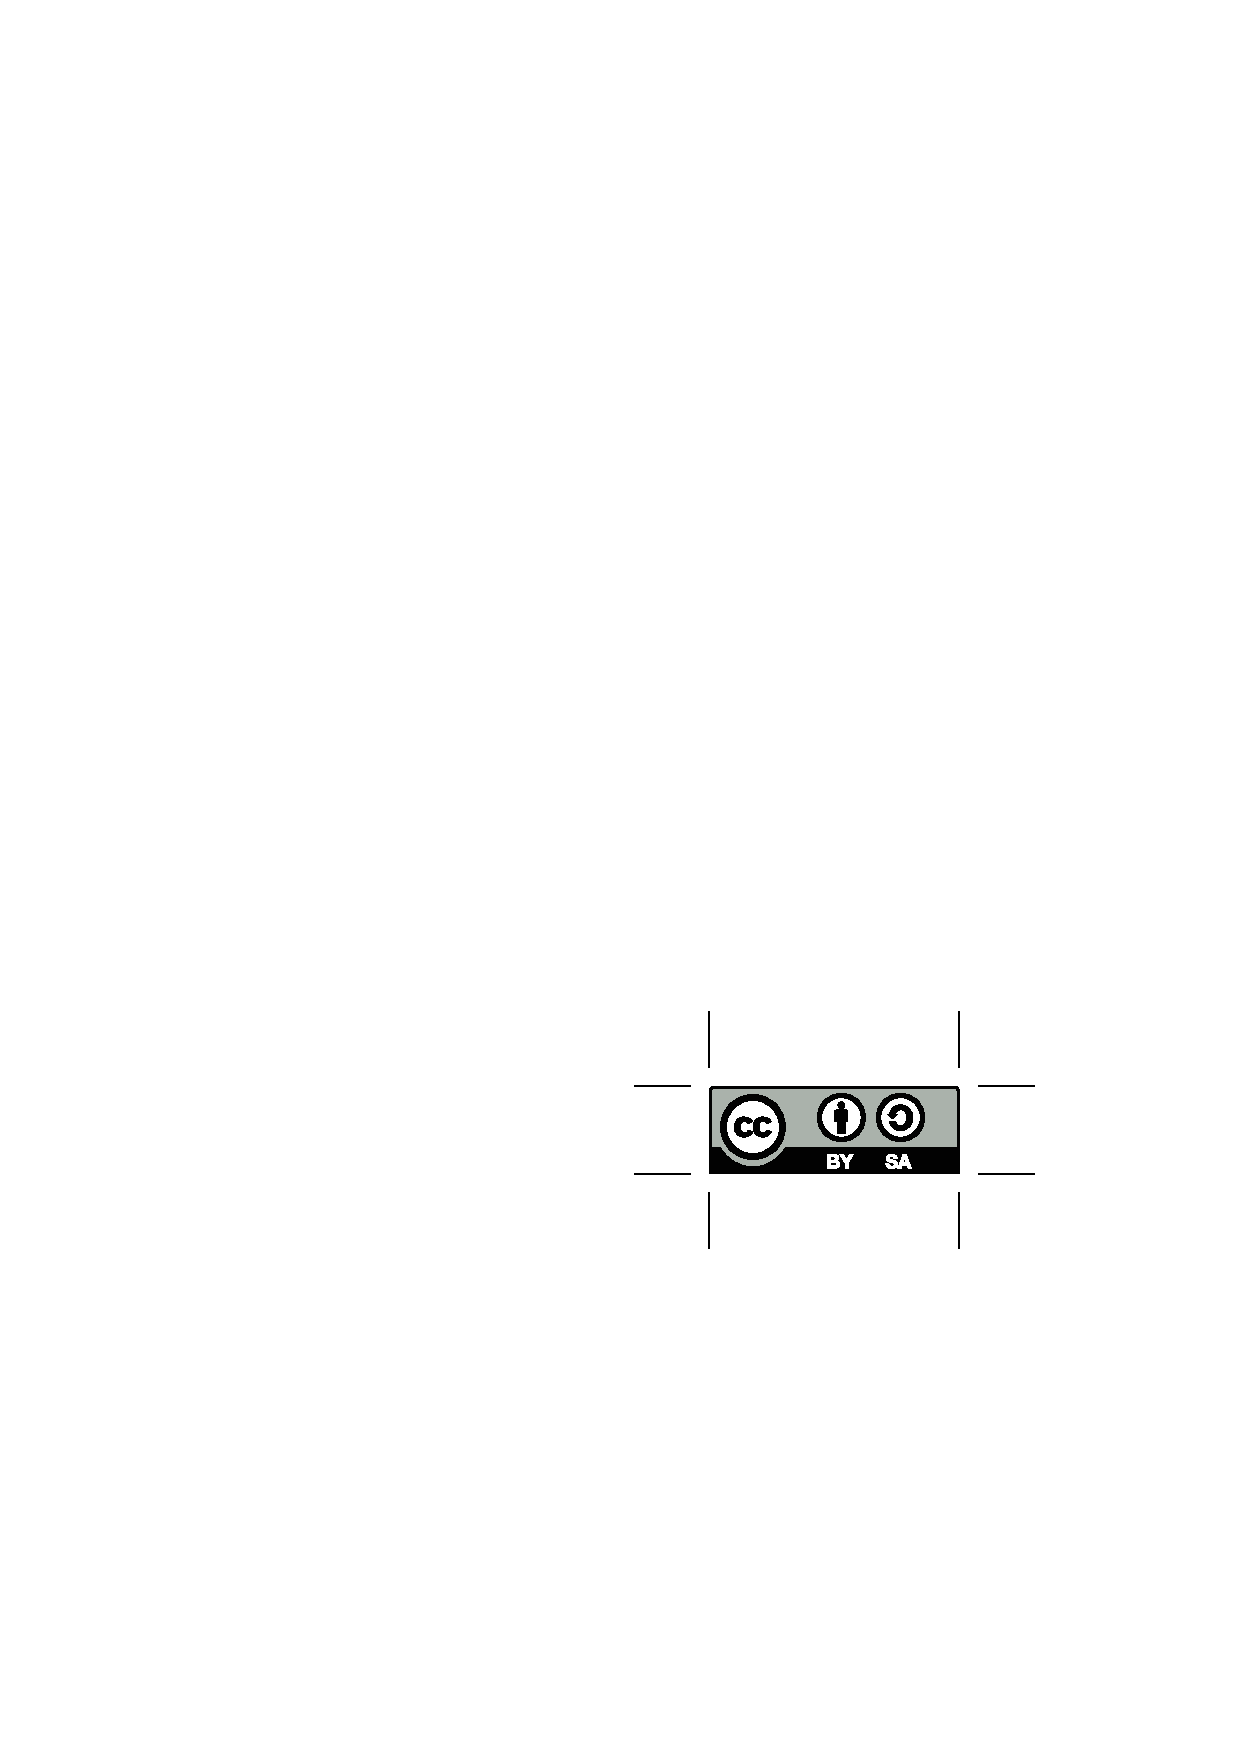
\includegraphics[scale=0.5]{pics/by-sa}
\vspace*{1mm}
\\
\hbox{\parbox{.7\textwidth}
{This work is licensed under the Creative Commons Attribution-ShareAlike
4.0 International License.
To view a copy of this license, visit\\
\texttt{http://creativecommons.org/licenses/by-sa/4.0/}}}

%\ 

%\noindent{\tt
%http://www.createspace.com/4122116
%\\
%\\
%ISBN-13: 978-1481918473
%\\
%ISBN-10: 1481918478
%}


\thispagestyle{empty}
\newpage
{\sloppy
\tableofcontents
}

\chapter*{Introduction}
\addcontentsline{toc}{chapter}{Introduction}
\addtocontents{toc}{\protect\begin{quote}}

This book is meant to be 
rigorous, 
conservative, 
elementary and
minimalist.
At the same time it includes about the maximum what students can absorb in one semester.

Approximately one-third of the material used to be covered in high school, but not any more.

The present book is based 
on the courses given by the author 
at the Pennsylvania State University
as an introduction to the foundations of geometry.
The lectures were oriented to sophomore and senior university students.  
These students already had a calculus course.
In particular, they are familiar with the real numbers and continuity.
It makes it possible to cover the material faster 
and  in a more rigorous way
than it could be done in high school.

\section*{Prerequisite}
\addtocontents{toc}{Prerequisite.}

The students should be familiar 
with the following topics.
\begin{itemize}
\item Elementary set theory: 
$\in$,
$\cup$, 
$\cap$,
$\backslash$,
$\subset$,~$\times$.
\item Real numbers: intervals, inequalities, algebraic identities.
\item Limits, continuous functions and the intermediate value theorem.
\item Standard functions: 
absolute value, 
natural logarithm,
exponential function. 
Occasionally, trigonometric functions  are used, 
but these parts can be ignored.
\item  Chapter~\ref{chap:trans} uses matrix algebra of $2{\times}2$-matrices.
\item To read Chapter~\ref{chap:sphere}, it is better to have some previous experience with the {}\emph{scalar product}, also known as {}\emph{dot product}.
\item To read Chapter~\ref{chap:complex}, it is better to have some previous experience with complex numbers.
\end{itemize} 

\section*{Overview}
\addtocontents{toc}{Overview.}

We use the so called {}\emph{metric approach} introduced by Birkhoff.
It means that we define the Euclidean plane as a {}\emph{metric space} which satisfies a list of properties ({}\emph{axioms}).
This way we minimize the tedious parts
which are unavoidable in the more classical Hilbert's approach.
At the same time the students have a chance to learn basic geometry of metric spaces.

Here is a dependency graph of the chapters.

\begin{figure}[h!]
\centering
\begin{tikzpicture}[->,>=stealth',shorten >=1pt,auto,scale=1.4,
  thick,main node/.style={circle,draw,font=\sffamily\bfseries,minimum size=8mm}]

  \node[main node] (1) at (1,15/6) {\ref{chap:metr}};
  \node[main node] (2) at (2,15/6){\ref{chap:axioms}};
  \node[main node] (3) at (3,15/6) {\ref{chap:half-planes}};
  \node[main node] (4) at (4,15/6) {\ref{chap:cong}};
  \node[main node] (5) at (3.5,10/6) {\ref{chap:perp}};
  \node[main node] (6) at (4.5,10/6) {\ref{chap:parallel}};
  \node[main node] (61) at (4,5/6) {\ref{chap:angle-sum}};
  \node[main node] (7) at (5,5/6) {\ref{chap:triangle}};
  \node[main node] (8) at (3,5/6){\ref{chap:inscribed-angle}};
  \node[main node] (9) at (2,5/6) {\ref{chap:inversion}};
  \node[main node] (10) at (2.5,10/6) {\ref{chap:non-euclid}};
  \node[main node] (11) at (1.5,10/6){\ref{chap:poincare}};
  \node[main node] (12) at (.5,10/6) {\ref{chap:h-plane}};
  \node[main node] (13) at (1.5,0) {\ref{chap:trans}};
  \node[main node] (14) at (0.5,0) {\ref{chap:proj}};
  \node[main node] (15) at (1,5/6) {\ref{chap:sphere}};
  \node[main node] (16) at (0,5/6) {\ref{chap:klein}};
  \node[main node] (17) at (2.5,0) {\ref{chap:complex}};
  \node[main node] (18) at (3.5,0) {\ref{chap:car}};
  \node[main node] (19) at (4.5,0) {\ref{chap:area}};

  \path[every node/.style={font=\sffamily\small}]
   (1) edge node[right]{}(2)
   (2) edge node[right]{}(3)
   (3) edge node[right]{}(4)
   (4) edge node[right]{}(5)
   (5) edge node[right]{}(6)
   (6) edge node[right]{}(61)
   (61) edge node[right]{}(8)
   (61) edge node[right]{}(7)
   (61) edge node[right]{}(19)
   (9) edge node[right]{}(13)
   (13) edge node[right]{}(14)
   (61) edge node[right]{}(18)
   (8) edge node[right]{}(9)
   (9) edge node[right]{}(11)
   (9) edge node[right]{}(15)
   (9) edge node[right]{}(17)
   (5) edge node[right]{}(10)
   (10) edge node[right]{}(11)
   (11) edge node[right]{}(12)
   (14) edge node[right]{}(16)
   (15) edge node[right]{}(16)
   (12) edge node[dashed,right]{}(16);
\end{tikzpicture}
\end{figure}


In (\ref{chap:metr}) we give all the definitions necessary to formulate the axioms;
it includes metric space, 
lines, 
angle measure, 
continuous maps and congruent triangles.


Further we do Euclidean geometry:
(\ref{chap:axioms}) Axioms and immediate corollaries;
(\ref{chap:half-planes}) Half-planes and continuity;
(\ref{chap:cong}) Congruent triangles;
(\ref{chap:perp}) Circles, motions, perpendicular lines;
(\ref{chap:parallel}) Similar triangles and (\ref{chap:angle-sum}) Parallel lines  
--- these are the first two chapters where we use Axiom \ref{def:birkhoff-axioms:4}, an equivalent of Euclid's parallel postulate.
In (\ref{chap:triangle}) we give the most classical theorem of triangle geometry;
this chapter is included mainly as an illustration.


In the following two chapters we discuss geometry of circles on the Euclidean plane:
(\ref{chap:inscribed-angle}) Inscribed angles; (\ref{chap:inversion}) Inversion.
It  will be used to construct the model of the hyperbolic plane.

Further 
we discuss non-Euclidean geometry:
(\ref{chap:non-euclid})
Neutral geometry --- geometry without the parallel postulate;
(\ref{chap:poincare})
Conformal disc model ---
this is a construction of the hyperbolic plane,
an example of a neutral plane which is not Euclidean.
In (\ref{chap:h-plane}) we discuss geometry of the constructed hyperbolic plane --- this is the highest point in the book.

In the reamining chapters we discuss some additional topics:
(\ref{chap:trans}) Affine geometry;
(\ref{chap:proj}) Projective geometry;
(\ref{chap:sphere}) Spherical geometry;
(\ref{chap:klein}) Projective model of the hyperbolic plane;
(\ref{chap:complex}) Complex coordinates;
(\ref{chap:car}) Geometric constructions;
(\ref{chap:area}) Area.
The proofs in these chapters are not completely rigorous.

We encourage to use the visual assignments available at the author's website.

\section*{Disclaimer}

It is  impossible to find the original reference to most of the theorems discussed here, so I do not even try to.
Most of the proofs discussed in the book 
already appeared in the Euclid's Elements.

\section*{Recommended books}

\begin{itemize}
\item Kiselev's textbook \cite{kiselev} ---
a classical book for school students.
Should help if you have trouble following this book.

\item Moise's book, \cite{moise} ---
should be good for further study.

\item Greenberg's book \cite{greenberg}  --- a historical tour in the axiomatic systems of various geometries.

\item Prasolov's book \cite{prasolov} is perfect to master your problem-solving skills.

\item Akopyan's book \cite{akopyan} --- a collection of problems formulated in figures.

\item Methodologically my lectures
were very close to Sharygin's  textbook \cite{sharygin}.
This is the greatest textbook in geometry for school students,
I recommend it to anyone who can read Russian.


\end{itemize}

\section*{Acknowlegments}

Let me thank  
Matthew Chao, 
Svetlana Katok, 
Alexander Lytchak,
Alexei Novi\-kov
and Lukeria Petrunina
for useful suggestions and correcting the misprints.






\addtocontents{toc}{\protect\end{quote}}


\chapter{Preliminaries}\label{chap:metr}
\addtocontents{toc}{\protect\begin{quote}}

\section*{What is the axiomatic approach?}
\addtocontents{toc}{What is the axiomatic approach?}

In the axiomatic approach,
one defines the plane as anything which satisfies 
a given list of properties.
These properties are called {}\emph{axioms}.
Axiomatic system for the theory 
is like the rules for a game.
Once the axiom system is fixed, a statement is considered to be true if it follows from the axioms and nothing else is considered to be true.

The formulations of the first axioms were not rigorous at all.
For example, Euclid described a {}\emph{line} as {}\emph{breadthless length}
and {}\emph{straight line} as a line which {}\emph{lies evenly with the points on itself}.
On the other hand,
these formulations were sufficiently clear, 
so that one mathematician could understand the other.

The best way to understand an axiomatic system
is to make one by yourself.
Look around and choose a physical model 
of the Euclidean plane;
imagine an infinite and perfect surface of a chalk board. 
Now try to collect the key observations
about this model.
Assume for now that we have intuitive understanding of such notions as {}\emph{line} and {}\emph{point}.
\begin{enumerate}[(i)]
 \item\label{preaxiomI} We can measure distances between points.
 \item\label{preaxiomII} We can draw a unique line 
 which passes thru two given points.
 \item\label{preaxiomIII} We can measure angles.
 \item\label{preaxiomIV} If we rotate or shift we will not see the difference.
 \item\label{preaxiomV} If we change scale we will not see the difference.
\end{enumerate}
These observations are good to start with.
Further we will develop the language
to reformulate them rigorously.

\section*{What is a model?}
\addtocontents{toc}{What is a model?}

The Euclidean plane can be defined rigorously the following way:

{}\emph{Define a {}\emph{point} in the Euclidean plane as a pair of real numbers $(x,y)$ and define the {}\emph{distance} between the two points $(x_1,y_1)$ and $(x_2,y_2)$ by the following formula:}
\[\sqrt{(x_1-x_2)^2+(y_1-y_2)^2}.\]

That is it!
We gave a {}\emph{numerical model} of Euclidean plane;
it builds the Euclidean plane from the real numbers
while the latter is assumed to be known.

Shortness is the main advantage of the model approach,
but it is not intuitively clear why we define points and the distances this way.

On the other hand, the observations made in the previous section are  intuitively obvious ---
this is the main advantage of the axiomatic approach.

An other advantage lies in the fact that the axiomatic approach is easily adjustable. 
For example, we may remove one axiom from the list,
or exchange it to another axiom. 
We will do such modifications in Chapter \ref{chap:non-euclid} and further.

\section*{Metric spaces}
\addtocontents{toc}{Metric spaces.}

The notion of metric space provides 
a rigorous way to say: {}\emph{``we can measure distances between points''}.
That is, instead of (\ref{preaxiomI}) on page \pageref{preaxiomI},
we can say {}\emph{``Euclidean plane is a metric space''}.

\begin{thm}{Definition}\label{def:metric-space}
Let $\mathcal X$ be a nonempty set and 
$d$ be a function
which returns a real number $d(A,B)$
for any pair $A,B\in\mathcal X$.
Then $d$
is called \index{metric}\emph{metric} on 
$\mathcal X$ if for any
$A,B,C\in \mathcal X$, the following conditions are satisfied.
\begin{enumerate}[(a)]
\item\label{def:metric-space:a} Positiveness: 
$$d(A,B)\ge 0.$$
\item\label{def:metric-space:b}  $A=B$ if and only if 
$$d(A,B)=0.$$
\item\label{def:metric-space:c} Symmetry: $$d(A, B) = d(B, A).$$
\item\label{def:metric-space:d} Triangle inequality: 
$$d(A, C) \le d(A, B) + d(B, C).$$
\end{enumerate}
A \index{metric space}\emph{metric space} is a set with a metric on it. 
More formally, a metric space is a pair $(\mathcal X, d)$ where $\mathcal X$ is a set and $d$ is a metric on~$\mathcal X$.

The elements of $\mathcal X$ are called \index{point}\emph{points} of the metric space.
Given two points $A,B\z\in \mathcal X$, 
the value $d(A, B)$ is called \index{distance}\emph{distance} from $A$ to~$B$.
\end{thm}

\section*{Examples}
\addtocontents{toc}{Examples.}

\begin{itemize}
\item {}\emph{Discrete metric.} Let $\mathcal X$ be an arbitrary set. 
For any $A,B\z\in\mathcal X$, 
set $d(A,B)\z=0$ if $A=B$ and $d(A,B)=1$ otherwise.
The metric $d$ is called \index{discrete metric}\emph{discrete metric} on~$\mathcal X$.
\item\index{real line}\emph{Real line.} Set of all real numbers ($\mathbb{R}$) with metric defined as 
$$d(A,B)\df|A-B|.$$
\item {}\emph{Metrics on the plane.}
Let us denote by $\mathbb{R}^2$ the set of all pairs $(x,y)$ of real numbers.
Assume $A=(x_A,y_A)$ and $B=(x_B,y_B)$ are arbitrary points in~$\mathbb{R}^2$.
One can equip $\mathbb{R}^2$ with the following metrics:
\begin{itemize}
\item\index{Euclidean metric}\emph{Euclidean metric,} denoted by \index{d@$d_1$, $d_2$, $d_\infty$}$d_2$ and defined as \label{def:d_2}
$$d_2(A,B)=\sqrt{(x_A-x_B)^2+(y_A-y_B)^2}.$$
\item\label{Manhattan plane}\index{Manhattan plane}\emph{Manhattan metric,} denoted by $d_1$ and defined as 
$$d_1(A,B)=|x_A-x_B|+|y_A-y_B|.$$
\item{}\emph{Maximum metric,} denoted by $d_\infty$ and defined as 
$$d_\infty(A,B)=\max\{|x_A-x_B|,|y_A-y_B|\}.$$
\end{itemize}
\end{itemize}

\begin{thm}{Exercise}\label{ex:d_1+d_2+d_infty}
Prove that the following functions are metrics on $\mathbb{R}^2$:
(a)~$d_1$; (b)~$d_2$; (c)~$d_\infty$.
\end{thm}


\section*{Shortcut for distance}
\addtocontents{toc}{Shortcut for distance.}

Most of the time,  
we study only one metric on the space.
Therefore, we will not need to name the metric function each time.

Given a metric space $\mathcal X$,
the distance between points $A$ and $B$ will be further denoted by 
$$AB
\quad
\text{or}
\quad
d_{\mathcal X}(A,B);$$
the latter is used only if we need to emphasize, that $A$ and $B$ are points of the metric space~$\mathcal X$.

For example, the triangle inequality can be written as 
$$AC\le AB+BC.$$

For the multiplication, we will always use ``$\cdot$'',
so $AB$ should not be confused with $A\cdot B$.

\section*{Isometries, motions and lines}
\addtocontents{toc}{Isometries, motions and lines.}

In this section, we define {}\emph{lines} in a metric space.
Once it is done the sentence  {}\emph{``We can draw a unique line which passes thru two given points.''} becomes rigorous; see (\ref{preaxiomII}) on page \pageref{preaxiomII}. 

Recall that a map $f\:\mathcal{X}\to\mathcal{Y}$
is a \index{bijection}\emph{bijection},
if it gives an exact pairing of the elements of two sets.
Equivalently, $f\:\mathcal{X}\to\mathcal{Y}$ is a bijection, if it has an \index{inverse}\emph{inverse};
that is, a map $g\:\mathcal{Y}\to\mathcal{X}$
such that 
$g(f(A))\z=A$   for any $A\in\mathcal{X}$
and
$f(g(B))\z=B$ for any $B\in\mathcal{Y}$. 

\begin{thm}{Definition}\label{def:isom}
Let $\mathcal X$ and $\mathcal Y$ be two metric spaces and $d_{\mathcal X}$, $d_{\mathcal Y}$ be their metrics. 
The map 
$$f\:\mathcal X \z\to \mathcal Y$$ 
is
called \index{distance-preserving map}\emph{distance-preserving} if 
$$d_{\mathcal Y}(f(A), f(B))
 = d_{\mathcal X}(A,B)$$
for any $A,B\in {\mathcal X}$.

A bijective distance-preserving map is called an \index{isometry}\emph{isometry}. 

Two metric spaces are called
\emph{isometric} if there exists an isometry from one to the other.

The isometry from a metric space to itself 
is also called a \index{motion}\emph{motion} of the space.
\end{thm}

\begin{thm}{Exercise}\label{ex:dist-preserv=>injective}
Show that any distance-preserving map  is \index{injective map}\emph{injective};
that is, if $f\:\mathcal X\to\mathcal Y$ is a distance-preserving map, 
then $f(A)\ne f(B)$ for any pair of distinct points $A,  B\in \mathcal X$.
\end{thm}

\begin{thm}{Exercise}\label{ex:motion-of-R}
Show that if $f\:\mathbb{R}\to\mathbb{R}$ is a motion of the real line,
then either (a)
$f(x)=f(0)+x$ for any $x\in \mathbb{R}$,  
or (b)
$f(x)=f(0)-x$ for any $x\in \mathbb{R}$. 

\end{thm}

\begin{thm}{Exercise}\label{ex:d_1=d_infty}
Prove that $(\mathbb{R}^2,d_1)$ is isometric to $(\mathbb{R}^2,d_\infty)$.
\end{thm}

\begin{thm}{Advanced exercise}\label{ad-ex:motions of Manhattan plane}
Describe all the motions of the Manhattan plane, defied on page~\pageref{Manhattan plane}.
\end{thm}

If $\mathcal X$ is a metric space and $\mathcal Y$ is a subset of $\mathcal X$,
then a metric on $\mathcal Y$ can be obtained by restricting the metric from~$\mathcal X$. 
In other words, 
the distance between two points of $\mathcal Y$ is defined to be the distance between these points in =~$\mathcal X$.
This way any subset of a metric space can be also considered as a metric space. 

\begin{thm}{Definition}\label{def:line}
A subset $\ell$ of metric space is called a \index{line}\emph{line}, if it is isometric to the real line.
\end{thm}

Note that a space with a discrete metric has no lines.
The following picture shows examples of lines on the Manhattan plane $(\mathbb{R}^2,d_1)$. 

\begin{center}
\begin{lpic}[t(0mm),b(0mm),r(0mm),l(0mm)]{pics/mink-lines(1)}
\end{lpic}
\end{center}

\begin{thm}{Exercise}\label{ex:y=|x|}
Consider the graph $y=|x|$ in =~$\mathbb{R}^2$.
In which of the following spaces 
(a) $(\mathbb{R}^2,d_1)$, 
(b) $(\mathbb{R}^2,d_2)$, 
(c) $(\mathbb{R}^2,d_\infty)$ 
does it form a line? 
Why?
\end{thm}

\begin{thm}{Exercise}\label{ex:2mid}
How many points $M$ are there on the line $(A B)$ for which we have
\begin{enumerate}
\item $AM= MB$ ?
\item $AM= 2\cdot MB$ ?
\end{enumerate}
\end{thm}

\section*{Half-lines and segments}
\addtocontents{toc}{Half-lines and segments.}

Assume there is a line $\ell$ passing thru
two distinct points $P$ and =~$Q$.
In this case we might denote $\ell$ as $(PQ)$.
There might be more than one line thru $P$ and $Q$,
but if we write \index{60@$(PQ)$, $[PQ)$, $[PQ]$}$(PQ)$ we assume that we made a choice of such line. 

Let us denote by $[P Q)$ the \index{half-line}\emph{half-line}
which starts at $P$ and contains~$Q$. 
Formally speaking, $[P Q)$ is a subset of $(P Q)$ which corresponds to $[0,\infty)$ under an isometry $f\:(P Q)\to \mathbb{R}$ such that $f(P)=0$ and $f(Q)>0$.

\begin{thm}{Exercise}\label{ex:trig==}
Show that if $X\in [PQ)$, then 
$QX=|PX-PQ|$.
\end{thm}

The subset of line $(P Q)$ between $P$ and $Q$ is called the \index{segment}\emph{segment} between $P$ and $Q$ and denoted by~$[P Q]$.
Formally, the segment can be defined as the intersection of two half-lines: $[P Q]=[P Q)\cap[Q P)$.


\section*{Angles}
\addtocontents{toc}{Angles.}

Our next goal is to introduce {}\emph{angles} and {}\emph{angle measures}; 
after that, the statement {}\emph{``we can measure angles''} will become rigorous;
see (\ref{preaxiomIII}) on page \pageref{preaxiomIII}.

\begin{wrapfigure}{r}{40mm}
\begin{lpic}[t(-4mm),b(-2mm),r(0mm),l(3mm)]{pics/angle(1)}
\lbl[rb]{2,5;$O$}
\lbl[rb]{16,25;$B$}
\lbl[b]{31,5;$A$}
\lbl[lb]{12,7;$\alpha$}
\end{lpic}
\end{wrapfigure}

An ordered pair of half-lines which start at the same point is called an \index{angle}\emph{angle}.
The angle $AOB$ (also denoted by \index{10@$\angle$}$\angle AOB$) is formed by two half-lines $[OA)$ and $[OB)$.
In this case the point $O$ is called the \index{vertex of the angle}\emph{vertex} of the angle.

Intuitively, the angle measure tells how much one has to rotate the first half-line counterclockwise, so it gets the position of the second half-line of the angle. 
The full turn is assumed to be $2\cdot\pi$;
it corresponds to the angle measure in radians.

The angle measure of $\angle AOB$ is denoted by \index{12@$\measuredangle$}$\measuredangle AOB$;
it is a real number in the interval $(-\pi,\pi]$. 

The notations $\angle AOB$ and $\measuredangle AOB$ look similar,
they also have close but different meanings, 
which better not be confused.
For example, the equality 
$\angle AOB=\angle A'O'B'$
means that
$[OA)=[O'A')$ and $[OB)\z=[O'B')$;
in particular, $O=O'$.
On the other hand the equality 
$\measuredangle AOB\z=\measuredangle A'O'B'$ 
means only equality of two real numbers;
in this case $O$ may be distinct from~$O'$.

Here is the first property of angle measure which will become a part of the axiom.

\textit{Given a half-line $[O A)$ and $\alpha\in(-\pi,\pi]$ there is a unique half-line $[O B)$ such that $\measuredangle A O B= \alpha$.}





\section*{Reals modulo $\bm{2\cdot\pi}$}
\addtocontents{toc}{Reals modulo $2\cdot\pi$.}

Consider three half-lines starting from the same point,
 $[O A)$, $[O B)$ and~$[O C)$.
They make three angles $A O B$, $B O C$ and $A O C$,
so the value $\measuredangle A O C$ should coincide with
the sum $\measuredangle A O B+\measuredangle B O C$ up to full rotation.
This property will be expressed by the formula 
$$\measuredangle A O B+\measuredangle B O C\equiv \measuredangle A O C,$$
where \index{34@$\equiv$}``$\equiv$'' is a new notation which we are about to introduce.
The last identity will become a part of the axiom.

%???how to say who is pi???

We will write 
\begin{align*}
\alpha&\equiv\beta
\intertext{or}
\alpha&\equiv\beta\pmod{2\cdot\pi}
\end{align*}
if $\alpha=\beta+2\cdot\pi\cdot n$
for some integer~$n$.
In this case we say 
$$\textit{``$\alpha$ is equal to $\beta$ modulo $2\cdot\pi$''}.$$
For example 
$$-\pi
\equiv
\pi\equiv 3\cdot\pi
\quad
\text{and}
\quad
\tfrac12\cdot\pi
\equiv
-\tfrac32\cdot\pi.$$

The introduced relation ``$\equiv$'' behaves as an equality sing,
but
\[\dots\equiv\alpha-2\cdot\pi\equiv \alpha\equiv \alpha+2\cdot\pi\equiv \alpha+4\cdot\pi\equiv\dots;\] 
that is, if the angle measures differ by full turn,
then they are considered to be the same.

With ``$\equiv$'', we can do addition, subtraction and multiplication with integer numbers without getting into trouble.
That is, if
$$\alpha\equiv\beta
\quad
\text{and}
\quad
\alpha'\equiv \beta',$$ 
then
$$\alpha+\alpha'\equiv\beta+\beta',
\quad
\alpha-\alpha'\equiv \beta-\beta'
\quad 
\text{and}
\quad
n\cdot\alpha\equiv n\cdot\beta$$
for any integer~$n$.
But ``$\equiv$'' does not in general respect multiplication with non-integer numbers; for example 
$$\pi
\equiv 
-\pi
\quad
\text{but}
\quad
\tfrac12\cdot\pi
\not\equiv
-\tfrac12\cdot\pi.$$ 

\begin{thm}{Exercise}\label{ex:2a=0}
Show that $2\cdot\alpha\equiv0$ if and only if $\alpha\equiv0$ or $\alpha\equiv\pi$.
\end{thm}

\section*{Continuity}
\addtocontents{toc}{Continuity.}

The angle measure is also assumed to be continuous.
Namely, the following property of angle measure will become a part of the axiom.

\textit{The function}
$$\measuredangle\:(A,O,B)\mapsto\measuredangle A O B$$
\textit{is continuous at any triple of points $(A,O,B)$
such that $O\ne A$ and $O\ne B$ and $\measuredangle A O B\ne\pi$.}

To explain this property, we need to extend the notion of {}\emph{continuity} to the functions between metric spaces.
The definition is a straightforward generalization of the standard definition for the real-to-real functions.

Further, let $\mathcal X$ and $\mathcal Y$ be two metric spaces,
and $d_{\mathcal X}$, $d_{\mathcal Y}$ be their metrics.

A map $f\:\mathcal X\to\mathcal Y$ is called continuous at point $A\in \mathcal X$
if for any  $\epsilon>0$ there is $\delta>0$, such that 
\[d_{\mathcal X}(A,A')
<
\delta
\quad
\Rightarrow
\quad
d_{\mathcal Y}(f(A),f(A'))
<
\epsilon.\]

One may define a continuous map of several variables the same way.
Assume $f(A,B,C)$ is a function which returns a point in the space $\mathcal Y$ for a triple of points $(A,B,C)$
in the space~$\mathcal X$.
The map $f$ might be defined only for some triples in~$\mathcal X$.

Assume $f(A,B,C)$ is defined.
Then, we say that $f$ is continuous at the triple $(A,B,C)$ 
if for any $\epsilon>0$ there is $\delta>0$ such that 
\[d_{\mathcal Y}(f(A,B,C),f(A',B',C'))<\epsilon.\]
if $d_{\mathcal X}(A,A')<\delta$, $d_{\mathcal X}(B,B')<\delta$ and $d_{\mathcal X}(C,C')<\delta$.


\begin{thm}{Exercise}\label{ex:dist-cont}
Let $\mathcal{X}$ be a metric space.
\begin{enumerate}[(a)]
\item\label{ex:dist-cont:a} Let $A\in \mathcal{X}$ be a fixed point.
Show that the function 
$$f(B)\df
d_{\mathcal{X}}(A,B)$$ 
is continuous at any point~$B$.
\item Show that $d_{\mathcal{X}}(A,B)$ is continuous  at any pair $A,B\in \mathcal{X}$.
\end{enumerate}

\end{thm}

\begin{thm}{Exercise}\label{ex:comp+cont}
Let $\mathcal{X}$, $\mathcal{Y}$ and $\mathcal{Z}$ be a metric spaces.
Assume that the functions $f\:\mathcal{X}\to\mathcal{Y}$
and $g\:\mathcal{Y}\to\mathcal{Z}$ are continuous at any point,
and $h=g\circ f$ is its composition;
that is, $h(A)=g(f(A))$ for any $A\in \mathcal{X}$.
Show that $h\:\mathcal{X}\to\mathcal{Z}$ is continuous at any point.
\end{thm}

\begin{thm}{Exercise}\label{ex:isom-cont}
Show that any distance-preserving map is continuous.
\end{thm}




\section*{Congruent triangles} 
\addtocontents{toc}{Congruent triangles.}

Our next goal is to give a rigorous meaning for  (\ref{preaxiomIV}) on page \pageref{preaxiomIV}.
To do this, we introduce the notion of {}\emph{congruent triangles}
so instead of {}\emph{``if we rotate or shift we will not see the difference''} we say that for triangles, the side-angle-side congruence holds;
that is, two triangles are congruent if they have two pairs of equal sides and the same angle measure between these sides.

An {}\emph{ordered} triple of distinct points in a metric space $\mathcal{X}$, 
say $A,B,C$,
is called a \index{triangle}\emph{triangle $ABC$}\label{page:def:triangle} (briefly  \index{20@$\triangle$}$\triangle A B C$).
Note that the triangles $A B C$ and $ A C B$ are considered as different.

Two triangles $ A' B' C'$ and $ A B C$ are called 
\index{triangle!congruent triangles}
\index{congruent triangles}\emph{congruent}
(written as \index{32@$\cong$}$\triangle A' B' C'\z\cong\triangle A B C$) if there is a motion $f\:\mathcal{X}\to\mathcal{X}$ such that 
\[A'\z=f(A),
\quad
B'=f(B)
\quad
\text{and}
\quad
C'=f(C).\]

Let $\mathcal X$ be a metric space,
and $f,g\:\mathcal X\to\mathcal X$ be two motions.
Note that the inverse $f^{-1}:\mathcal X\to\mathcal X$,
as well as the composition $f\circ g:\mathcal X\to\mathcal X$
are also motions.

It follows that ``$\cong$'' is an \index{equivalence relation}\emph{equivalence relation};
that is, any triangle congruent to itself, 
and the following two conditions hold.
\begin{itemize} 
\item If $\triangle A' B' C'\z\cong\triangle A B C$, then $\triangle A B C\z\cong\triangle A' B' C'$.
\item If $\triangle A'' B'' C''\z\cong\triangle A' B' C'$ and $\triangle A' B' C'\z\cong\triangle A B C$,
then 
$$\triangle A'' B'' C''\cong\triangle A B C.$$
\end{itemize}


Note that if $\triangle A' B' C'\z\cong\triangle A B C$,
then $AB\z=A'B'$,
$BC=B'C'$ and $CA=C'A'$.

For a discrete metric, as well as some other metrics, 
the converse also holds.
The following example shows that it does not hold in the Manhattan plane.

\parbf{Example.}\label{example:isometric but not congruent} Consider three points 
$A=(0,1)$, $B=(1,0)$ and $C\z=(-1,0)$ on the Manhattan plane $(\mathbb{R}^2,d_1)$.
Note that
$$d_1(A,B)=d_1(A,C)=d_1(B,C)=2.$$

\begin{wrapfigure}[7]{o}{46mm}
\begin{lpic}[t(-3mm),b(0mm),r(0mm),l(2mm)]{pics/mink-ABC(1)}
\lbl[b]{21,23;$A$}
\lbl[lt]{37,4;$B$}
\lbl[rt]{6,4;$C$}
\end{lpic}
\end{wrapfigure}

On one hand,
$$\triangle ABC\cong \triangle ACB.$$

Indeed, 
it is easy to see that
 the map $(x,y)\mapsto (-x,y)$ is a motion of $(\mathbb{R}^2,d_1)$,
which sends $A\mapsto A$, $B\mapsto C$ and $C\mapsto B$.

On the other hand,
$$\triangle ABC\z\ncong \triangle BCA.$$

%???(
Indeed, arguing by contradiction, assume that $f$ is a motion of $(\mathbb{R}^2,d_1)$ which sends $A\mapsto B$ and $B\mapsto C$.
%???)
Note that a point $M$ is a midpoint\footnote{$M$ is a midpoint of $A$ and $B$ if $d_1(A,M)=d_1(B,M)=\tfrac12\cdot d_1(A,B)$.} of $A$ and $B$ if and only if $f(M)$ is a midpoint of $B$ and~$C$.

The set of midpoints for $A$ and $B$ is infinite, it contains all points $(t,t)$ for $t\in[0,1]$ (it is the dark gray segment on the picture above).
On the other hand, the midpoint for $B$ and $C$ is unique (it is the black point on the picture).
Thus, the map $f$ cannot be bijective, a contradiction.

\addtocontents{toc}{\protect\end{quote}}
%\part*{Euclidean geometry}
\addtocontents{toc}{\protect\begin{center}}
\addtocontents{toc}{\large{\bf Euclidean geometry}}
\addtocontents{toc}{\protect\end{center}}
\chapter{Axioms}
\label{chap:axioms}
\addtocontents{toc}{\protect\begin{quote}}

%(???

\vfill

A system of axioms appears already in Euclid's ``Elements'' --- the most successful and influential textbook ever written.

The systematic study of geometries as axiomatic systems
 was
triggered by the discovery of non-Euclidean geometry.
The branch of mathematics, emerging this way, is called ``Foundations of geometry''.

The most popular system of axiom
was proposed in 1899 by David Hilbert.
This is also the first rigorous system by modern standards.
It contains twenty axioms in five groups, six ``primitive notions'', and three ``primitive terms'';
these are not defined in terms of previously defined concepts.

Later a number of different systems were proposed.
It is worth mentioning
the system of Alexandr Alexandrov \cite{alexandrov} which is very intuitive and elementary, 
the system of Friedrich Bachmann \cite{bachmann} which is based on the concept of symmetry,
and the system of Alfred Tarski \cite{tarski}, which was designed for analysis using mathematical logic.

We will use another system,
which is very close to the one proposed by George Birkhoff in \cite{birkhoff}.
This system is based on the {}\emph{key observations}  (\ref{preaxiomI})--(\ref{preaxiomV}) listed on page~\pageref{preaxiomI}.
The axioms use the notions of 
metric space, 
lines, 
angles,
triangles,
equalities modulo $2\cdot\pi$ ($\equiv$), 
the continuity of maps between metric spaces,
and the congruence of triangles ($\cong$).
All this discussed in the preliminaries.

Our system is build upon metric spaces.
In particular, we use the real numbers as a building block. 
By that reason our approach is not purely axiomatic --- we build the theory upon something else;
it resembles a model-based introduction to Euclidean geometry discussed on page~\pageref{page:model}.
We used this approach to minimize the tedious parts which are unavoidable in purely axiomatic foundations.

%???)

\newpage

\section*{The axioms}
\addtocontents{toc}{The axioms.}

\begin{framed}
\begin{enumerate}[I.]
\item\label{def:birkhoff-axioms:0} The \index{plane!Euclidean plane}\index{Euclidean plane}\emph{Euclidean plane} is a metric space with at least two points.


\item\label{def:birkhoff-axioms:1} 
There is one and only one line, that contains any two given distinct points $P$ and $Q$ in the Euclidean plane.

\item\label{def:birkhoff-axioms:2} 
Any angle $AOB$ in the Euclidean plane 
defines a real number in the interval $(-\pi,\pi]$.
This number is called \index{angle measure}\emph{angle measure of $\angle AOB$}
and denoted by $\measuredangle A O B$.
It satisfies the following conditions:
\begin{enumerate}[(a)]
\item\label{def:birkhoff-axioms:2a} 
Given a half-line $[O A)$ and $\alpha\in(-\pi,\pi]$, 
there is a unique  half-line $[O B)$, 
such that $\measuredangle A O B= \alpha$.
\item\label{def:birkhoff-axioms:2b} 
For any points $A$, $B$, and $C$, distinct from $O$ we have
$$\measuredangle A O B+\measuredangle B O C
\equiv\measuredangle A O C.$$
\item\label{def:birkhoff-axioms:2c} 
The function 
$$\measuredangle\:(A,O,B)\mapsto\measuredangle A O B$$
is continuous at any triple of points $(A,O,B)$,
such that $O\ne A$ and $O\ne B$ and $\measuredangle A O B\ne\pi$.

\end{enumerate}

\item\label{def:birkhoff-axioms:3}  
In the Euclidean plane, we have
$\triangle A B C\cong\triangle A' B' C'$
if and only if 
\begin{align*}
A' B'&=A B, & A' C'&= A C, &&\text{and}
&\measuredangle C' A' B'&=\pm\measuredangle C A B.
\end{align*}
\item\label{def:birkhoff-axioms:4}
If for two triangles $ABC$, $AB'C'$ in the Euclidean plane
and for $k>0$ we have
\begin{align*}
B'&\in [AB),
& C'&\in [AC),
\\
AB'&=k\cdot AB,&
AC'&=k\cdot AC,
\end{align*}
then
\begin{align*}
B'C'&=k\cdot BC,&
\measuredangle ABC&=\measuredangle AB'C',
&
\measuredangle ACB&=\measuredangle AC'B'.
\end{align*}
\end{enumerate}
\end{framed}

From now on,  
we can use no information about the Euclidean plane which does not follow from the five axioms above.

\begin{thm}{Exercise}\label{ex:infinite}
Show that there are (a) an infinite set of points,
(b) an infinite set of lines on the plane.
\end{thm}

\section*{Lines and half-lines}
\addtocontents{toc}{Lines and half-lines.}

\begin{thm}[\abs]{Proposition}\label{lem:line-line}
\let\thefootnote\relax\footnotetext{${}^\a$ A statement marked with ``$\a$'' if Axiom~\ref{def:birkhoff-axioms:4} was not used in its proof.
Ignore this mark for a while; it will be important in Chapter~\ref{chap:non-euclid}, see page \pageref{a-mark}.}
Any two distinct lines intersect at most at one point.
\end{thm}

\parit{Proof.}
Assume that two lines $\ell$ and $m$ intersect at two distinct points $P$ and~$Q$.
Applying Axiom~\ref{def:birkhoff-axioms:1}, we get that $\ell=m$.
\qeds

\begin{thm}{Exercise}\label{ex:[OA)=[OA')}
Suppose $A'\in[OA)$ and $A'\not=O$. 
Show that 
\[[O A)\z=[O A').\]

\end{thm}

\begin{thm}[\abs]{Proposition}\label{prop:point-on-half-line}
Given $r\ge 0$ and a half-line $[O A)$ there is a unique $A'\in [O A)$  such that $O A'=r$.
\end{thm}

\parit{Proof.}
According to definition of half-line, 
there is an isometry 
$$f\:[O A)\to [0,\infty),$$
such that $f(O)=0$.
By the definition of isometry, $O A'=f(A')$ for any $A'\z\in [O A)$.
Thus, $O A'=r$ if and only if $f(A')=r$.

Since isometry has to be bijective, the statement follows.
\qeds

\section*{Zero angle}
\addtocontents{toc}{Zero angle.}

\begin{thm}[\abs]{Proposition}\label{lem:AOA=0}
$\measuredangle A O A= 0$ for any $A\not=O$.
\end{thm}

\parit{Proof.}
According to Axiom~\ref{def:birkhoff-axioms:2b},
$$\measuredangle A O A
+
\measuredangle A O A 
\equiv
\measuredangle A O A.$$
Subtract  $\measuredangle A O A$ from both sides, we get that
$\measuredangle A O A \equiv 0$.

By Axiom~\ref{def:birkhoff-axioms:2}, $-\pi<\measuredangle A O A\le \pi$;
therefore $\measuredangle A O A \z= 0$.
\qeds

\begin{thm}{Exercise}\label{ex:2.4} 
Assume $\measuredangle A O B= 0$.
Show that $[OA)=[OB)$.
\end{thm}

\begin{thm}[\abs]{Proposition}\label{lem:AOB+BOA=0}
For any $A$ and $B$ distinct from $O$,
we have 
$$\measuredangle A O B\equiv-\measuredangle B O A.$$

\end{thm}

\parit{Proof.}
According to Axiom~\ref{def:birkhoff-axioms:2b},
$$\measuredangle A O B+\measuredangle B O A \equiv\measuredangle A O A$$
By Proposition~\ref{lem:AOA=0}, $\measuredangle A O A=0$.
Hence the result.
\qeds

\section*{Straight angle}
\addtocontents{toc}{Straight angle.}

If $\measuredangle A O B=\pi$,
we say that $\angle A O B$ is a 
\index{angle!straight angle}\emph{straight angle}.
Note that by Proposition~\ref{lem:AOB+BOA=0}, 
if $\angle A O B$ is a straight,
then so is $\angle B O A$.

We say that point $O$ \index{between}\emph{lies between} points $A$ and $B$, 
if $O\not= A$, $O\not= B$, and $O\in[A B]$.

\begin{thm}[\abs]{Theorem}\label{thm:straight-angle}
The angle $A O B$ is straight 
if and only if $O$ 
\index{between}\emph{lies between} $A$ and~$B$.
\end{thm}

\begin{wrapfigure}{r}{39mm}
\centering
\includegraphics{mppics/pic-8}
\end{wrapfigure}

\parit{Proof.}
By Proposition~\ref{prop:point-on-half-line},  we may assume that
$O A = O B = 1$.

\parit{``If'' part.}
Assume $O$  
lies between $A$ and~$B$.
Set  $\alpha=\measuredangle A O B$.

Applying Axiom~\ref{def:birkhoff-axioms:2a},
we get a half-line $[OA')$ such that $\alpha\z=\measuredangle B O A'$.
By Proposition~\ref{prop:point-on-half-line}, we can assume that $OA'=1$.
According to Axiom~\ref{def:birkhoff-axioms:3},
\[\triangle AOB\z\cong\triangle BOA'.\]
Let $f$ denotes the corresponding motion of the plane;
that is, $f$ is a motion such that $f(A)=B$, $f(O)=O$, and $f(B)=A'$. 

\begin{wrapfigure}{o}{39mm}
\centering
\includegraphics{mppics/pic-10}
\end{wrapfigure}

Then 
\[(A'B)=f(AB)\ni f(O)=O.\]
Therefore, both lines $(AB)$ and $(A'B)$ contain $B$ and~$O$.
By Axiom~\ref{def:birkhoff-axioms:1}, $(AB)=(A'B)$.

By the definition of the line,
$(AB)$ contains exactly two points $A$ and $B$ on distance $1$ from~$O$.
Since $OA'=1$ and $A'\ne B$, we get that $A=A'$.

By Axiom~\ref{def:birkhoff-axioms:2b} and Proposition~\ref{lem:AOA=0}, we get that
\begin{align*}
2\cdot\alpha&=
\measuredangle AOB+\measuredangle BOA'=
\\
&=\measuredangle AOB+\measuredangle BOA\equiv
\\
&\equiv\measuredangle AOA=
\\
&= 0
\end{align*}
Therefore, by Exercise~\ref{ex:2a=0}, $\alpha$ is either $0$ or~$\pi$.

Since $[OA)\ne [OB)$,  
we have that $\alpha\ne 0$, see Exercise~\ref{ex:2.4}.
Therefore, $\alpha=\pi$.


\parit{``Only if'' part.}
Suppose that $\measuredangle A O B= \pi$.
Consider the line $(OA)$ and choose a point $B'$ on $(OA)$ so that $O$ lies between $A$ and~$B'$.

From above, we have that $\measuredangle AOB'=\pi$.
Applying Axiom~\ref{def:birkhoff-axioms:2a}, 
we get that $[O B)\z=[O B')$.
In particular, $O$ lies between $A$ and~$B$.
\qeds 

A triangle $ABC$ is called 
\index{triangle!degenerate triangle}\index{degenerate! triangle}\emph{degenerate}
if $A$, $B$, and $C$ lie on one line.
The following corollary is just a reformulation of Theorem~\ref{thm:straight-angle}.

\begin{thm}[\abs]{Corollary}\label{cor:degenerate=pi}
A triangle is degenerate if and only if one of its angles is equal to $\pi$ or~$0$.
Moreover in a degenerate triangle the angle measures are $0$, $0$, and $\pi$.
\end{thm}

\begin{thm}{Exercise}\label{ex:lineAOB}
Show that three distinct points $A$, $O$, and $B$ lie on one line if and only if 
$$2\cdot \measuredangle AOB\equiv 0.$$ 

\end{thm}

\begin{thm}{Exercise}\label{ex:ABCO-line}
Let $A$, $B$ and $C$ be three points distinct from~$O$.
Show that $B$, $O$ and $C$ lie on one line if and only if
$$2\cdot \measuredangle AOB\equiv 2\cdot \measuredangle AOC.$$ 

\end{thm}

\begin{thm}{Exercise}\label{ex:infinite-number-of-lines} 
Show that there is a nondegenerate triangle.
\end{thm}

\section*{Vertical angles}
\addtocontents{toc}{Vertical angles.}

A pair of angles $AOB$ and $A'OB'$ 
is called \index{angle!vertical angles}\index{vertical angles}\emph{vertical}
if the point $O$ 
lies between $A$ and $A'$ 
and between $B$ and $B'$ at the same time.


\begin{thm}[\abs]{Proposition}\label{prop:vert}
The vertical angles have equal measures.
\end{thm}


\parit{Proof.}
Assume that the angles $AOB$ and $A'OB'$ are vertical.
Note that $\angle AOA'$ and $\angle BOB'$ are straight.
Therefore, $\measuredangle AOA'\z=\measuredangle BOB'=\pi$.

{

\begin{wrapfigure}[4]{o}{24mm}
\vskip-2mm
\centering
\includegraphics{mppics/pic-12}
\end{wrapfigure}

It follows that
\begin{align*}
0&=\measuredangle AOA'-\measuredangle BOB'\equiv
\\
&\equiv 
\measuredangle AOB+\measuredangle BOA'-\measuredangle BOA'-\measuredangle A'OB'
\equiv
\\
&\equiv\measuredangle AOB-\measuredangle A'OB'.
\end{align*}
Since $-\pi<\measuredangle AOB\le \pi$ and $-\pi<\measuredangle A'OB'\le \pi$, we get that $\measuredangle AOB\z=\measuredangle A'OB'$.
\qeds

}

\begin{thm}{Exercise}\label{ex:O-mid-AB+CD}
Assume $O$ 
is the midpoint for both segments 
$[A B]$ and $[C D]$.
Prove that $A C= B D$. 
\end{thm}




\addtocontents{toc}{\protect\end{quote}}

\chapter{Half-planes}\label{chap:half-planes}
\addtocontents{toc}{\protect\begin{quote}}

This chapter contains long proofs of intuitively evident statements.
It is okay to skip it, but make sure you know definitions of positive/negative angles and that your intuition agrees with \ref{thm:signs-of-triug}, \ref{prop:half-plane}, \ref{cor:half-plane}, \ref{thm:pasch} and \ref{thm:abc}.

 
                            
\section*{Sign of an angle}
\addtocontents{toc}{Sign of an angle.}

The positive and negative angles can be visualized as {}\emph{counterclockwise} and  {}\emph{clockwise} directions; formally, they are defined the following way.

\begin{itemize}
\item The angle $A O B$ is called \index{angle!positive and negative angles}\emph{positive} 
if $0<\measuredangle A O B<\pi$;
\item The  angle $A O B$ is called {}\emph{negative} 
if $\measuredangle A O B<0$.
\end{itemize}

Note that according to the above definitions the straight angle as well as the zero angle 
are neither positive nor negative.

\begin{thm}{Exercise}\label{ex:AOB+<=>BOA-}
Show that $\angle A O B$ is positive if and only if $\angle B O A$ is negative.
\end{thm}

\begin{thm}{Lemma}\label{lem:straight-sign}
Let $\angle AOB$ be straight.
Then $\angle AOX$ is positive 
if and only if $\angle BOX$ is negative.
\end{thm}

\parit{Proof.}
Set $\alpha=\measuredangle AOX$ 
and 
$\beta=\measuredangle BOX$.
Since $\angle AOB$ is straight,
$$\alpha-\beta\equiv \pi.\eqlbl{eq:alpha-beta}$$

It follows that $\alpha=\pi$ $\Leftrightarrow$ $\beta=0$
and $\alpha=0$ $\Leftrightarrow$ $\beta=\pi$.
In these two cases the sing of $\angle AOX$ and $\angle BOX$ are undefined.

In the remaining cases we have $|\alpha|,|\beta|<\pi$.
If $\alpha$ and $\beta$ have the same sign, then $|\alpha-\beta|<\pi$;
the latter contradicts \ref{eq:alpha-beta}.
Hence the statement follows.
\qeds

\begin{thm}{Exercise}\label{ex:PP(PN)}
Assume that the angles $AOB$ and $BOC$ are positive. 
Show that
$$\measuredangle AOB+\measuredangle BOC+\measuredangle COA=2\cdot\pi.$$
if $\angle COA$ is positive,
and
$$\measuredangle AOB+\measuredangle BOC+\measuredangle COA=0.$$
if $\angle COA$ is negative.
\end{thm}




\section*{Intermediate value theorem}
\addtocontents{toc}{Intermediate value theorem.}


\begin{thm}{Intermediate value theorem}\label{thm:intermidiate}
Let $f\:[a,b]\to \mathbb{R}$ be a continuous function.
Assume 
$f(a)$ and $f(b)$ have opposite signs,
then $f(t_0)=0$ for some $t_0\in[a,b]$.
\end{thm}

\begin{wrapfigure}{o}{38mm}
\begin{lpic}[t(-6mm),b(0mm),r(0mm),l(5mm)]{pics/ivt(1)}
\lbl[r]{2,20;$f(b)$}
\lbl[r]{2,1;$f(a)$}
\lbl[tl]{11,8;$t_0$}
\lbl[t]{27.5,8;$b$}
\lbl[b]{7.5,10.5;$a$}
\end{lpic}
\end{wrapfigure}



The intermediate value theorem is assumed to be known;
it should be covered in any calculus course.
We will use the following corollary.

\begin{thm}[\abs]{Corollary}\label{cor:intermidiate}
Assume that for any $t\z\in [0,1]$ we have three points in the plane  $O_t$, $A_t$ and $B_t$, such that 
\begin{enumerate}[(a)]
\item Each  function $t\mapsto O_t$, $t\mapsto A_t$ and $t\mapsto B_t$ is continuous.
\end{enumerate}

\begin{enumerate}[(a)]\addtocounter{enumi}{1}
\item For for any $t\in [0,1]$, the points $O_t$, $A_t$ and $B_t$ do not lie on one line.  
\end{enumerate}
Then $\angle A_0O_0B_0$ and $\angle A_1O_1B_1$ have the same sign.
\end{thm}

\parit{Proof.}
Consider the function 
$f(t)=\measuredangle A_tO_tB_t$.

Since 
the points $O_t$, $A_t$ and $B_t$ do not lie on one line,
Theorem~\ref{thm:straight-angle} implies that $f(t)=\measuredangle A_tO_tB_t\ne 0$ nor $\pi$ for any $t\in[0,1]$.

Therefore, by Axiom~\ref{def:birkhoff-axioms:2c} and Exercise~\ref{ex:comp+cont},
$f$ is a continuous function.

Further,
by the intermediate value theorem, $f(0)$ and $f(1)$ have the same sign;
hence the result follows.
\qeds

\section*{Same sign lemmas}
\addtocontents{toc}{Same sign lemmas.}

\begin{thm}[\abs]{Lemma}\label{lem:signs}
Assume $Q'\in [PQ)$ and $Q'\z\ne P$.
Then for any $X\z\notin (PQ)$ the angles $PQX$ and $PQ'X$ have the same sign. 
\end{thm}

\begin{wrapfigure}{o}{33mm}
\begin{lpic}[t(-0mm),b(1mm),r(0mm),l(0mm)]{pics/PQX(1)}
\lbl[t]{30,1;$P$}
\lbl[t]{18,1;$Q'$}
\lbl[t]{1,1;$Q$}
\lbl[r]{11,27;$X$}
\end{lpic}
\end{wrapfigure}

\parit{Proof.}
By Proposition~\ref{prop:point-on-half-line},
for any $t\in [0,1]$ there is a unique point $Q_t\in[PQ)$ 
such that 
\[PQ_t=  (1-t)\cdot PQ+t\cdot PQ'.\]
Note that the map $t\mapsto Q_t$ is continuous,
\begin{align*}
Q_0&=Q,
&
Q_1&=Q'
\end{align*}
and for any $t\in [0,1]$, 
we have $P\z\ne Q_t$.

Applying Corollary \ref{cor:intermidiate},
for $P_t=P$, $Q_t$ and $X_t=X$, we get that $\angle PQX$ has the same sign as $\angle PQ'X$.
\qeds



\begin{thm}[\abs]{Signs of angles of a triangle}\label{thm:signs-of-triug}
In any nondegenerate triangle $ABC$,
the angles $ABC$, $BCA$ and $CAB$ have the same sign. 
\end{thm}

{

\begin{wrapfigure}{o}{33mm}
\begin{lpic}[t(-3mm),b(1mm),r(0mm),l(0mm)]{pics/PQX-2(1)}
\lbl[t]{30,1;$Z$}
\lbl[t]{18,1;$A$}
\lbl[t]{2,1;$B$}
\lbl[b]{12.5,28.5;$C$}
\end{lpic}
\end{wrapfigure}

\parit{Proof.}
Choose a point $Z\in (AB)$ so that $A$ lies between $B$ and~$Z$.


According to Lemma~\ref{lem:signs},
the angles $ZBC$ and $ZAC$ have the same sign.


Note that $\measuredangle ABC=\measuredangle ZBC$
and 
$$\measuredangle ZAC+\measuredangle CAB\equiv \pi.$$
Therefore, $\angle CAB$ has the same sign as $\angle ZAC$
which in turn has the same sign as $\measuredangle ABC\z=\measuredangle ZBC$.

}

Repeating the same argument for $\angle BCA$ and $\angle CAB$,
we get the result.
\qeds

\begin{thm}[\abs]{Lemma}\label{lem:signsXY}
Assume $[XY]$ does not intersect $(PQ)$,
then the angles $PQX$ and $PQY$ 
have the same sign.
\end{thm}

\begin{wrapfigure}{r}{34mm}
\begin{lpic}[t(-5mm),b(3mm),r(0mm),l(0mm)]{pics/PQY(1)}
\lbl[t]{30,1;$P$}
\lbl[t]{1,1;$Q$}
\lbl[r]{11,27;$X$}
\lbl[l]{24,13;$Y$}
\end{lpic}
\end{wrapfigure}

The proof is nearly identical to the one above.

\parit{Proof.}
According to Proposition~\ref{prop:point-on-half-line},
for any $t\in [0,1]$ there is a point  $X_t\in[XY]$, 
such that 
\[XX_t= t\cdot XY.\]
Note that the map $t\mapsto X_t$ is continuous.
Moreover, $X_0=X$, $X_1=Y$ and $X_t\notin(QP)$ for any $t\in [0,1]$.

Applying Corollary \ref{cor:intermidiate},
for $P_t\z=P$, $Q_t\z=Q$ and $X_t$, we get that
$\angle PQX$ has the same sign as $\angle PQY$.
\qeds



\section*{Half-planes}
\addtocontents{toc}{Half-planes.}

%(???

\begin{thm}{Proposition}\label{prop:half-plane}
Assume $X,Y\notin(PQ)$.
Then the angles $PQX$ and $PQY$ have the same sign if and only if $[XY]$ does not intersect $(PQ)$.
\end{thm}

\begin{wrapfigure}{o}{30mm}
\begin{lpic}[t(-4mm),b(-0mm),r(0mm),l(0mm)]{pics/PQXYZ(1)}
\lbl[b]{11,14;$Q$}
\lbl[b]{3,13.3;$P$}
\lbl[l]{28,24;$X$}
\lbl[l]{27,1;$Y$}
\lbl[lt]{27,11;$Z$}
\end{lpic}
\end{wrapfigure}

\parit{Proof.} The if-part follows from Lemma~\ref{lem:signs}. 

Assume $[XY]$ intersects $(PQ)$;
let $Z$ denotes the point of intersection.
Without loss of generality, we can assume $Z\ne P$.

Note that $Z$ lies between $X$ and $Y$.
By Lemma~\ref{lem:straight-sign}, $\angle PZX$ and $\angle PZY$ have opposite signs.
This proves the statement if $Z=Q$.

If $Z\ne Q$, then $\angle ZQX$ and $\angle QZX$ have opposite signs by \ref{thm:signs-of-triug}.
The same way we get that $\angle ZQY$ and $\angle QZY$ have opposite signs.

If $Q$ lies between $Z$ and $P$, then by Lemma~\ref{lem:straight-sign} two pairs of angles $\angle PQX$, $\angle ZQX$ and $\angle PQY$, $\angle ZQY$ have opposite signs. 
It follows that $\angle PQX$ and $\angle PQY$ have opposite signs as required.

In the remaining case $[QZ)=[QP)$ and therefore $\angle PQX=\angle ZQX$ and $\angle PQY=\angle ZQY$. 
Hence again $\angle PQX$ and $\angle PQY$ have opposite signs as required.
\qeds

%)???

\begin{thm}[\abs]{Corollary}\label{cor:half-plane}
The complement of a line $(PQ)$ in the plane 
can be presented in a unique way as a union of two disjoint subsets 
called \index{half-plane}\emph{half-planes}
such that 
\begin{enumerate}[(a)]
\item\label{cor:half-plane:angle} Two points $X,Y\notin(PQ)$ lie in the same half-plane if and only if the angles $PQX$ and $PQY$ have the same sign.
\item\label{cor:half-plane:intersect} Two points $X,Y\notin(PQ)$ lie in the same half-plane if and only if $[XY]$ does not intersect~$(PQ)$.
\end{enumerate}

\end{thm}

\begin{wrapfigure}[6]{o}{25mm}
\begin{lpic}[t(-3mm),b(-5mm),r(0mm),l(0mm)]{pics/vert-intersect(1)}
\lbl[l]{10.5,13.5;$O$}
\lbl[tr]{20,3;$A$}
\lbl[t]{7.5,8.5;$B$}
\lbl[b]{6,17.5;$A'$}
\lbl[tl]{19,24;$B'$}
\end{lpic}
\end{wrapfigure}

We say that $X$ and $Y$ lie on  {}\emph{one side from} $(PQ)$ if they lie in one of the half-planes of $(PQ)$ and we say that  $P$ and $Q$ lie on the {}\emph{opposite sides from} $\ell$ if they lie in the different half-planes of~$\ell$.


\begin{thm}{Exercise}\label{ex:vert-intersect}
Assume that the angles $AOB$ and $A'OB'$ are vertical.
Show that the line $(AB)$ does not intersect the segment~$[A'B']$.
\end{thm}


Consider the triangle $ABC$.
The segments $[AB]$, $[BC]$ and $[CA]$ are called 
\index{side!side of the triangle}\emph{sides of the triangle}.

The following theorem follows from Corollary~\ref{cor:half-plane}.

{

\begin{wrapfigure}{o}{21mm}
\begin{lpic}[t(-0mm),b(-5mm),r(0mm),l(0mm)]{pics/pasch(1)}
\lbl[tr]{1,1;$A$}
\lbl[b]{7,18.5;$B$}
\lbl[tl]{19,4;$C$}
\lbl[b]{18,12;$\ell$}
\end{lpic}
\end{wrapfigure}

\begin{thm}[\abs]{Pasch's theorem}\label{thm:pasch}
Assume line $\ell$ does not pass thru any vertex a triangle.
Then it intersects either two or zero sides of the triangle.
\end{thm}

\parit{Proof.}
Assume that line $\ell$ intersects side $[AB]$ of the triangle $ABC$ and does not pass thru $A$, $B$ and $C$.

}

By Corollary~\ref{cor:half-plane}, the vertexes $A$ and $B$ lie on opposite sides from $\ell$.

The vertex $C$ may lie on the same side with $A$ and on opposite side with $B$ or the other way around.
By Corollary~\ref{cor:half-plane}, in the first case $\ell$ intersects side $[BC]$ and does not intersect $[AC]$ and in the second case $\ell$ intersects side $[AC]$ and does not intersect $[BC]$.
Hence the statement follows.
\qeds

\begin{thm}{Exercise}\label{ex:signs-PXQ-PYQ}
Show that two points $X,Y\notin(PQ)$ lie on the same side from $(PQ)$
if and only if the angles $PXQ$ and $PYQ$ have the same sign.
\end{thm}

\begin{multicols}{2}
\begin{center}
\begin{lpic}[t(0mm),b(0mm),r(0mm),l(0mm)]{pics/PQY-1(1)}
\lbl[t]{30,1;$P$}
\lbl[t]{1,1;$Q$}
\lbl[b]{12,28.5;$X$}
\lbl[rb]{17,12;$Y$}
\end{lpic}
\end{center}
\columnbreak
\begin{center}
\begin{lpic}[t(-4mm),b(0mm),r(0mm),l(0mm)]{pics/PQY-2(1)}
\lbl[t]{30,1;$B$}
\lbl[t]{1,1;$A$}
\lbl[lb]{23,15;$A'$}
\lbl[rb]{8,19;$B'$}
\lbl[b]{12,28.5;$C$}
\end{lpic} 
\end{center}
\end{multicols}

\begin{thm}{Exercise}\label{ex:chevinas}
Let $\triangle ABC$ be a nondegenerate triangle,
$A'\in[BC]$  and 
$B'\in [AC]$.
Show that the segments $[AA']$ and $[BB']$ intersect.
\end{thm}

\begin{thm}{Exercise}\label{ex:Z}
Assume that the points $X$ and $Y$ lie on opposite sides from the line~$(PQ)$.
Show that the half-line $[PX)$ does not intersect~$[QY)$. 
\end{thm}

\begin{thm}{Advanced exercise}\label{ex:angle-measures}
Note that the following quantity 
$$\tilde\measuredangle ABC=\left[
\begin{aligned}
&\pi&&\text{if}&\measuredangle ABC&=\pi
\\
-&\measuredangle ABC&&\text{if}&\measuredangle ABC&<\pi
\end{aligned}
\right.$$
can serve as the angle measure; 
that is, the axioms hold if one exchanges $\measuredangle$ to $\tilde\measuredangle$ everywhere.

Show that $\measuredangle$ and $\tilde\measuredangle$ are the only possible angle measures on the plane. 

Show that without Axiom \ref{def:birkhoff-axioms:2c}, this is no longer true.
\end{thm}
 


\section*{Triangle with the given sides}
\addtocontents{toc}{Triangle with the given sides.}

Consider the triangle $ABC$.
Set 
\begin{align*}
a&=BC,
&
b&=CA,
&
c&=AB.
\end{align*}
Without loss of generality, we may assume that 
\[a\le b \le c.\]
Then all three triangle inequalities for $\triangle ABC$
hold if and only if 
\[c\le a+b.\]
The following theorem states that this is the only restriction on $a$, $b$ and~$c$.

\begin{thm}[\abs]{Theorem}\label{thm:abc}
Assume that $0<a\le b\le c\le a+b$.
Then there is a triangle $ABC$ 
such that $a=BC$, $b=CA$ and $c=AB$.
\end{thm}

The proof requires some preparation;
it is given in the end of section.

Assume $r>0$ and $\pi>\beta>0$.
Consider the triangle $ABC$ such that 
$AB=BC=r$ and $\measuredangle ABC=\beta$.
The existence of such a triangle follows from Axiom~\ref{def:birkhoff-axioms:2a} and Proposition~\ref{prop:point-on-half-line}.

\begin{wrapfigure}{o}{25mm}
\begin{lpic}[t(2mm),b(4mm),r(0mm),l(0mm)]{pics/sbr(1)}
\lbl[t]{2,0;$A$}
\lbl[t]{22,0;$C$}
\lbl[b]{12.5,29;$B$}
\lbl[w]{12.5,2.5;$\,s(\beta,r)\,$}
\lbl[W]{7.5,13;$r$}
\lbl[W]{19,13;$r$}
\lbl[t]{12.5,20;$\beta$}
\end{lpic}
\end{wrapfigure}

Note that according to Axiom~\ref{def:birkhoff-axioms:3}, 
the values
$\beta$ and $r$ define the triangle $ABC$ up to the congruence.
In particular, the distance $AC$ depends only on $\beta$ and~$r$.
Set 
$$s(\beta,r)\df AC.$$

\begin{thm}[\abs]{Proposition}\label{prop:f(r,a)}
Given $r>0$ and $\epsilon>0$, there is $\delta>0$ such that
if $0<\beta<\delta$, then 
\[s(r,\beta)<\epsilon.\]

\end{thm}


{

\begin{wrapfigure}{o}{33mm}
\begin{lpic}[t(-0mm),b(0mm),r(0mm),l(0mm)]{pics/fra(1)}
\lbl[t]{22.5,0;$A$}
\lbl[t]{2.5,0;$B$}
\lbl[b]{20,14;$C$}
\lbl[tl]{25,7;$D$}
\lbl[tl]{30,8;$Z$}
\lbl[r]{28,20;$Y$}
\lbl[rb]{30,27;$X$}
\lbl[w]{15,2;$\,r\,$}
\lbl[w]{13,8,30;$\,r\,$}
\end{lpic}
\end{wrapfigure}

\parit{Proof.}
Fix two points $A$ and $B$ such that $AB=r$.

Choose a point $X$ such that $\measuredangle ABX$ is positive.
Let $Y\in [AX)$ be the point such that $AY=\tfrac\epsilon8$;
it exists by Proposition~\ref{prop:point-on-half-line}.

Note that $X$ and $Y$ lie on the same side from $(AB)$;
therefore, $\angle ABY$ is positive. 
Set $\delta=\measuredangle ABY$.

Assume $0<\beta<\delta$,
$\measuredangle ABC=\beta$
and $BC\z=r$.




Applying Axiom~\ref{def:birkhoff-axioms:2a},
we can choose a half-line $[BZ)$ such that $\measuredangle ABZ=\tfrac12\cdot \beta$.
Note that $A$ and $Y$ lie on opposite sides from~$(BZ)$.
Therefore, $(BZ)$ intersects $[AY]$;
let $D$ denotes the point of intersection.

Since $D\in (BZ)$, we get that $\measuredangle ABD=\tfrac \beta2$ or $\tfrac\beta2-\pi$.
The latter is impossible since $D$ and $Y$ lie on the same side from~$(AB)$.
Therefore, 
$$\measuredangle ABD=\measuredangle DBC=\tfrac \beta2.$$



By Axiom~\ref{def:birkhoff-axioms:3},
$\triangle ABD\cong \triangle CBD$.
In particular,
\begin{align*}
AC&\le AD+DC=
\\
&=2\cdot AD\le 
\\
&\le 2\cdot AY=
\\
&=\tfrac\epsilon4
\end{align*}
and hence the result.
\qeds

}

\begin{thm}[\abs]{Corollary}\label{cor:C-cont}
Fix a real number $r>0$ 
and two distinct points $A$ and~$B$.
Then for 
any real number $\beta\in [0,\pi]$,
there is a unique point $C_\beta$ such that $BC_\beta=r$
and $\measuredangle ABC_\beta=\beta$.
Moreover, the map $\beta\mapsto C_\beta$ 
is a continuous map from $[0,\pi]$ to the plane.
\end{thm}

\parit{Proof.}
The existence and uniqueness of $C_\beta$ follows from Axiom~\ref{def:birkhoff-axioms:2a} and Proposition~\ref{prop:point-on-half-line}.

Note that if $\beta_1\ne\beta_2$, then
$$C_{\beta_1}C_{\beta_2}=s(r,|\beta_1-\beta_2|).$$

Therefore, Proposition~\ref{prop:f(r,a)} implies that  the map $\beta\mapsto C_\beta$ is continuous.
\qeds





\parit{Proof of Theorem~\ref{thm:abc}.}\label{page:proof:thm:abc}
Fix the points $A$ and $B$ such that $AB=c$.
Given $\beta\in [0,\pi]$,
let $C_\beta$ denotes the point in the plane such that $BC_\beta\z=a$ and $\measuredangle ABC=\beta$.

According to Corollary~\ref{cor:C-cont},
the map
$\beta\mapsto C_\beta$ is continuous.
Therefore, the function $b(\beta)=AC_\beta$ is continuous
(formally, it follows from Exercise~\ref{ex:dist-cont} and Exercise~\ref{ex:comp+cont}).

Note that $b(0)=c-a$ and $b(\pi)=c+a$.
Since $c-a\le b\le c+a$,
by the intermediate value theorem (\ref{thm:intermidiate})
there is $\beta_0\in[0,\pi]$ such that
$b(\beta_0)=b$.
Hence the result. 
\qeds



\addtocontents{toc}{\protect\end{quote}}
\chapter{Congruent triangles}\label{chap:cong}
\addtocontents{toc}{\protect\begin{quote}}

\section*{Side-angle-side condition}
\addtocontents{toc}{Side-angle-side condition.}

Our next goal is to give conditions which guarantee congruence of two triangles.
One of such conditions is Axiom~\ref{def:birkhoff-axioms:3}, it is also called \index{side-angle-side condition}\emph{side-angle-side condition} or briefly \index{SAS condition}\emph{SAS condition}.

\section*{Angle-side-angle condition}
\addtocontents{toc}{Angle-side-angle condition.}

\begin{thm}{ASA condition}\label{thm:ASA}\index{ASA congruence condition}\index{angle-side-angle congruence condition}
Assume that 
\begin{align*}
AB&=A'B',
&
\measuredangle A B C &\equiv \pm\measuredangle A' B' C', 
&
\measuredangle C A B&\equiv\pm\measuredangle C' A' B'
\end{align*}
 and $\triangle A' B' C'$ is nondegenerate.
Then 
$$\triangle A B C\cong\triangle A' B' C'.$$

\end{thm}

Note that for degenerate triangles the statement does not hold,
say consider one triangle with sides $1$, $4$, $5$ 
and the other with sides $2$, $3$,~$5$.

\begin{wrapfigure}[7]{o}{26mm}
\begin{lpic}[t(-0mm),b(3mm),r(0mm),l(0mm)]{pics/AA(1)}
\lbl[t]{1,.5;$A'$}
\lbl[b]{10.5,29;$B'$}
\lbl[t]{16,.5;$C'$}
\lbl[lt]{21,.5;$C''$}
\end{lpic}
\end{wrapfigure}

\parit{Proof.} 
According to Theorem~\ref{thm:signs-of-triug},
either
$$\begin{aligned}
 \measuredangle A B C &\equiv \measuredangle A' B' C',
\\
\measuredangle C A B&\equiv\measuredangle C' A' B'
\end{aligned}\eqlbl{eq:+angles}$$
or
$$\begin{aligned}
\measuredangle A B C &\equiv -\measuredangle A' B' C',
\\
\measuredangle C A B&\equiv-\measuredangle C' A' B'.
\end{aligned}\eqlbl{eq:-angles}$$
Further we assume that \ref{eq:+angles} holds; 
the case \ref{eq:-angles} is analogous.



Let $C''$ be the point on the half-line $[A' C')$ such that 
that $A' C''\z=A C$. 

By Axiom~\ref{def:birkhoff-axioms:3}, 
$\triangle A' B' C''\cong \triangle A B C$. 
Applying Axiom~\ref{def:birkhoff-axioms:3} again,
we get 
$$\measuredangle A' B' C'' \equiv  \measuredangle A B C\equiv\measuredangle A' B' C' .$$
By Axiom~\ref{def:birkhoff-axioms:2a}, $[B'C')=[B C'')$. 
Whence
$C''$ lies on $(B' C')$ as well as on $(A' C')$.

Since $\triangle A' B' C'$ is not degenerate, $(A' C')$ is distinct from $(B' C')$.
Applying  Axiom~\ref{def:birkhoff-axioms:1}, we get $C''=C'$. 

Therefore 
$\triangle A' B' C'=\triangle A' B' C''\cong\triangle A B C$.
\qeds

\section*{Isosceles triangles}
\addtocontents{toc}{Isosceles triangles.}

A triangle with two equal sides is called \index{isosceles triangle}\emph{isosceles};
the remaining side is called \index{base of isosceles triangle}\emph{base} of isosceles triangle.

\begin{thm}{Theorem}\label{thm:isos}
Assume $\triangle A B C$ is an isosceles triangle with the base $[A  B]$. 
Then 
$$\measuredangle A B C\equiv -\measuredangle B A C.$$
Moreover, the converse holds if $\triangle A B C$ is nondegenerate.
\end{thm}

\begin{wrapfigure}{o}{29mm}
\begin{lpic}[t(0mm),b(0mm),r(0mm),l(2mm)]{pics/isos(1)}
\lbl[rt]{0,1;$A$}
\lbl[lt]{23,1;$B$}
\lbl[b]{11.5,27;$C$}
\end{lpic}
\end{wrapfigure}

The following proof is due to Pappus of Alexandria.

\parit{Proof.}
Note that
$$C A = C B,\ C B=C A,\ \measuredangle A C B \equiv -\measuredangle B C A.$$
Therefore by Axiom~\ref{def:birkhoff-axioms:3},
$$\triangle C A B\cong\triangle C B A.$$
Applying the theorem on the signs of angles of triangles (\ref{thm:signs-of-triug}) and Axiom~\ref{def:birkhoff-axioms:3} again,
we get  
$$\measuredangle C A B\equiv -\measuredangle C B A.$$

To prove the converse, we assume
$\measuredangle C A B \z\equiv - \measuredangle C B A$.
By ASA condition \ref{thm:ASA}, $\triangle C A B\z\cong\triangle CBA$.
Therefore $C A\z=C B$.
\qeds

A triangle with three equal sides is called\index{equilateral triangle}\emph{equilateral}. 

\begin{thm}{Exercise}\label{ex:equilateral}
Let $\triangle ABC$ be an equilateral triangle.
Show that 
\[\measuredangle ABC=\measuredangle BCA=\measuredangle CAB.\]

\end{thm}


\section*{Side-side-side condition}
\addtocontents{toc}{Side-side-side condition.}
\index{side-side-side congruence condition}

\begin{thm}{SSS condition}\label{thm:SSS}
$\triangle A B C\cong\triangle A' B' C'$  if  
$$A' B'=A B,\ \ B' C'=B C\ \ \text{and}\ \  C' A'=C A.$$

\end{thm}

\parit{Proof.} 
Choose $C''$ so that $A' C''= A' C'$ and $\measuredangle B' A' C''\equiv \measuredangle B A C$.
According to Axiom~\ref{def:birkhoff-axioms:3},
$$\triangle A' B' C''\cong\triangle A B C.$$

\begin{wrapfigure}{o}{40mm}
\begin{lpic}[t(0mm),b(0mm),r(0mm),l(2mm)]{pics/SSS(1)}
\lbl[r]{1.5,20.5;$A'$}
\lbl[l]{35.5,20.5;$B'$}
\lbl[b]{24,40.5;$C'$}
\lbl[t]{24,1;$C''$}
\end{lpic}
\end{wrapfigure}

It will suffice to
prove that 
$$\triangle A' B' C'\cong\triangle  A' B' C''.\eqlbl{eq:A'B'C'simA'B'C''}$$
The condition \ref{eq:A'B'C'simA'B'C''} trivially holds if $C''\z=C'$.
Thus it remains to consider the case $C''\z\ne C'$.

Clearly, the corresponding  sides of $\triangle A' B' C'$ and $\triangle  A' B' C''$ are equal.
Whence the triangles
$\triangle C' A' C''$ and $\triangle C' B' C''$ are  isosceles.
By Theorem~\ref{thm:isos}, we have 
\begin{align*}
 \measuredangle A' C'' C'&\equiv  -\measuredangle A' C' C'',
\\
\measuredangle C' C'' B'&\equiv    -\measuredangle    C'' C' B'.
\end{align*}
By addition
$$\measuredangle  A' C' B' \equiv    -\measuredangle     A' C'' B'.$$
Applying Axiom~\ref{def:birkhoff-axioms:3} again,
we get \ref{eq:A'B'C'simA'B'C''}.
\qeds

\begin{thm}{Advanced exercise}\label{ex:SMS}
Let $M$ be the midpoint of side $[A B]$ of a triangle $\triangle A B C$ and
$M'$ be the midpoint of side $[A' B']$ of a triangle $\triangle A' B' C'$.
Assume $C' A'=C A$, $C' B'= C B$ and $C' M'= C M$.
Prove that $\triangle A' B' C'\cong\triangle A B C$.
\end{thm}

\begin{wrapfigure}[3]{o}{34mm}
\begin{lpic}[t(-8mm),b(-0mm),r(0mm),l(1mm)]{pics/isos-2(1)}
\lbl[t]{30,1;$B$}
\lbl[t]{1,1;$A$}
\lbl[lb]{26,13;$A'$}
\lbl[rb]{7,13;$B'$}
\lbl[b]{16,28.5;$C$}
\end{lpic}
\end{wrapfigure}

\begin{thm}{Exercise}\label{ex:isos-sides}
Let $\triangle A B C$ be an isosceles triangle with the base $[A B]$
and the points $A'\in [B C]$ and $B'\z\in[A C]$ be such that $C A'=C B'$.
Show that
\begin{enumerate}[(a)]
\item $\triangle A A' C\cong \triangle B B' C$;
\item $\triangle A B B'\cong \triangle B A A'$.
\end{enumerate}
\end{thm}



\begin{thm}{Exercise}\label{ex:degenerate-trig}
Show that if $AB+BC=AC$
 then $B\in [AC]$.
\end{thm}

\begin{thm}{Exercise}\label{ex:ABC-motion}
Let $\triangle ABC$ be a nondegenerate triangle and 
let $\iota$ be a motion of the plane 
such that 
$$\iota(A)=A,\ \ \iota(B)=B\ \ \text{and}\ \ \iota(C)=C.$$

Show that $\iota$ is the identity;
that is, $\iota(X)=X$ for any point $X$ on the plane.
\end{thm}




\addtocontents{toc}{
{\sloppy

}
\protect\end{quote}}
\chapter{Perpendicular lines}\label{chap:perp}
\addtocontents{toc}{\protect\begin{quote}}

\section*{Right, acute and obtuse angles}
\addtocontents{toc}{Right, acute and obtuse angles.}

\begin{itemize}
\item If $|\measuredangle A O B|=\tfrac\pi2$, we say that $\angle A O B$ is  \index{angle!right angle}\emph{right};
%\item If $\measuredangle A O B\ne\pm\tfrac\pi2$, we say that the angle  $\angle A O B$ is  \index{angle!oblique angle}\emph{oblique};
\item If $|\measuredangle A O B|<\tfrac\pi2$, we say that  $\angle A O B$ is  
\index{acute!angle}\emph{acute};
\item If $|\measuredangle A O B|>\tfrac\pi2$, we say that $\angle A O B$ is  \index{angle!acute and obtuse angles}\index{obtuse angle}\emph{obtuse}.
\end{itemize}

\begin{wrapfigure}{o}{30mm}
\begin{lpic}[t(-0mm),b(0mm),r(0mm),l(2mm)]{pics/perp-notation(1)}
\end{lpic}
\end{wrapfigure}

On the diagrams,
the right angles will be marked with a little square, 
as shown.

If $\angle A O B$ is right,
we say also
that $[O A)$ is \index{perpendicular}\emph{perpendicular} to $[O B)$; 
it will be written as \index{38@$\perp$}$[O A)\z\perp [O B)$.

From Theorem~\ref{thm:straight-angle}, 
it follows that two lines $(O A)$
 and $(O B)$ are appropriately called {}\emph{perpendicular}, if  $[O A)\z\perp [O B)$.
In this case we also write $(O A)\z\perp (O B)$.



\begin{thm}{Exercise}\label{ex:acute-obtuce}
Assume point $O$ lies between $A$ and $B$ and $X\ne O$.
Show that 
$\angle XOA$ is acute if and only if 
$\angle XOB$ is obtuse.
\end{thm}



\section*{Perpendicular bisector}
\addtocontents{toc}{Perpendicular bisector.}

Assume $M$ is the midpoint of the segment $[AB]$;
that is, $M\in(A B)$ and $A M \z=  M B$.

The line $\ell$ which passes thru $M$ and perpendicular to $(AB)$,
is called the \index{bisector!perpendicular bisector}\index{perpendicular bisector}\emph{perpendicular bisector} to the segment~$[AB]$. 

\begin{thm}[\abs]{Theorem}\label{thm:perp-bisect}
Given distinct points $A$ and $B$,
all points equidistant from $A$ and $B$ and no
others lie on the perpendicular bisector to~$[A B]$.
\end{thm}

\begin{wrapfigure}{o}{40mm}
\begin{lpic}[t(-0mm),b(0mm),r(0mm),l(0mm)]{pics/perp-bisect(1)}
\lbl[t]{2,7;$A$}
\lbl[t]{38,7;$B$}
\lbl[tl]{20.5,7;$M$}
\lbl[lb]{20.5,36;$P$}
\end{lpic}
\end{wrapfigure}

\parit{Proof.} Let $M$ be the midpoint of~$[A B]$.

Assume $P A= P B$ and $P\ne M$.
According to SSS (\ref{thm:SSS}),
$\triangle A M P \z\cong\triangle B M P$.
Hence 
$$\measuredangle A M P=\pm \measuredangle B M P.$$   
Since $A\not=B$, we have ``$-$'' in the above formula.
Further,
\begin{align*}
\pi
&=
\measuredangle A M B
\equiv
\\
&\equiv\measuredangle A M P+\measuredangle P M B
\equiv
\\
&\equiv
2\cdot \measuredangle A M P.
\end{align*}
That is, $\measuredangle A M P
=
\pm
\tfrac\pi2$. 
Therefore, $P$ lies on the perpendicular bisector.


To prove the converse, 
suppose $P$ 
is any point on the perpendicular bisector to $[A B]$ and $P\ne M$.
Then $\measuredangle A M P=\pm \tfrac\pi2$, 
$\measuredangle B M P=\pm \tfrac\pi2$ and
$A M\z=B M$.
Therefore, $\triangle A M P\cong \triangle B M P$;
in particular, $A P\z= B P$.\qeds


\begin{thm}{Exercise}\label{ex:pbisec-side}
Let $\ell$ be the perpendicular bisector to the segment $[A B]$ and $X$ be an arbitrary point on the plane.

Show that 
$AX<BX$ if and only if $X$ and $A$ lie on the same side from~$\ell$.
\end{thm}

\begin{thm}{Exercise}\label{ex:side-angle}
Let $\triangle ABC$ be nondegenerate.
Show that $AC>BC$ if and only if $|\measuredangle ABC|>|\measuredangle CAB|$.  
\end{thm}



\section*{Uniqueness of a perpendicular}
\addtocontents{toc}{Uniqueness of perpendicular lines.}

\begin{thm}[\abs]{Theorem}\label{perp:ex+un}
There is one and only one line  which passes thru a given point $P$ and is perpendicular to a given line~$\ell$.
\end{thm}

According to the above theorem, 
there is a unique point $Q\in\ell$ such that $(QP)\perp\ell$.
This point $Q$ is called the \index{foot point}\emph{foot point} of $P$ on~$\ell$. 

\parit{Proof.} 
If $P\in\ell$, then both, existence and uniqueness, follow from Axiom~\ref{def:birkhoff-axioms:2}.

\parit{Existence for $P\not\in\ell$.} 
Let $A$ and $B$ be two distinct points of~$\ell$. 
Choose $P'$ so that $AP'\z=AP$ and $\measuredangle P' A B\equiv -\measuredangle P A B$.
According to Axiom~\ref{def:birkhoff-axioms:3}, $\triangle A P' B\z\cong\triangle A P B$.
Therefore, $A P= A P'$ and $B P= B P'$.

{

\begin{wrapfigure}{o}{36mm}
\begin{lpic}[t(-0mm),b(-3mm),r(0mm),l(0mm)]{pics/perp(1)}
\lbl[rb]{1.5,18;$A$}
\lbl[lb]{33,18;$B$}
\lbl[t]{15,16;$\ell$}
\lbl[lb]{23,33;$P$}
\lbl[lt]{23,2;$P'$}
\end{lpic}
\end{wrapfigure}


According to Theorem~\ref{thm:perp-bisect}, $A$ and $B$ lie on the perpendicular bisector to~$[P P']$.
In particular, $(P P')\perp (A B)=\ell$.

\parit{Uniqueness for $P\not\in\ell$.} 
From above we can choose a point $P'$ in such a way that $\ell$ forms the perpendicular bisector to~$[PP']$.

Assume $m\perp \ell$ and $m\ni P$.
Then $m$ is a perpendicular bisector to some segment $[Q Q']$ of $\ell$;
in particular, $P Q= P Q'$.

}

{

\begin{wrapfigure}{i}{36mm}
\begin{lpic}[t(-2mm),b(-0mm),r(0mm),l(0mm)]{pics/perp-unique(1)}
\lbl[rb]{2,16;$Q$}
\lbl[lb]{33,16;$Q'$}
\lbl[lb]{18.5,28;$P$}
\lbl[lt]{18.5,2;$P'$}
\lbl[t]{14,14;$\ell$}
\lbl[b]{17,20,90;$m$}
\end{lpic}
\end{wrapfigure}

Since $\ell$ is the perpendicular bisector to $[P P']$,
we get that $PQ= P'Q$ and $PQ' = P'Q'$.
Therefore, 
$$P' Q=P Q=P Q'= P' Q'.$$
By Theorem~\ref{thm:perp-bisect}, 
$P'$ lies on the perpendicular bisector to $[QQ']$, which is~$m$.
By Axiom~\ref{def:birkhoff-axioms:1}, $m=(P P')$.
\qeds

}

\section*{Reflection}
\addtocontents{toc}{Reflection.}

Assume the point $P$ and the line $(AB)$ are given.
To find the \index{reflection}\emph{reflection} $P'$ of $P$ in $(AB)$,
one drops a perpendicular from $P$ onto $(AB)$, 
and continues it to the same distance on the other side.

According to Theorem~\ref{perp:ex+un}, $P'$ is uniquely determined by~$P$.

Note that $P=P'$ if and only if $P\in(AB)$.

\begin{thm}[\abs]{Proposition}\label{prop:reflection}
Assume $P'$ is a reflection of the point $P$ in the line~$(AB)$.
Then $AP'=AP$ 
and if $A\ne P$, 
then
$\measuredangle BAP'\equiv -\measuredangle BAP$.
\end{thm}

\parit{Proof.} 
Note that if $P\in (AB)$, 
then $P\z=P'$. 
By Corollary~\ref{cor:degenerate=pi}, $\measuredangle BAP=0$ or~$\pi$.
Hence the statement follows.

{
\begin{wrapfigure}{o}{43mm}
\begin{lpic}[t(-2mm),b(8mm),r(0mm),l(0mm)]{pics/reflection(1)}
\lbl[rb]{2,24;$A$}
\lbl[lb]{39,24;$B$}
\lbl[lb]{24.5,43.5;$P$}
\lbl[lt]{24.5,2.5;$P'$}
\end{lpic}
\end{wrapfigure}

If $P\notin (AB)$, then~$P'\ne P$.
By the construction of $P'$, 
the line $(AB)$ is perpendicular bisector of~$[PP']$.
Therefore, according to Theorem~\ref{thm:perp-bisect}, $AP'\z=AP$ and $BP'\z=BP$.
In particular, 
$\triangle ABP'\cong \triangle ABP$.
Therefore, $\measuredangle BAP'=\pm \measuredangle BAP$.

Since $P'\ne P$ and $AP'=AP$,
we get that $\measuredangle BAP'\ne \measuredangle BAP$.
That is, we are left with the case
$$\measuredangle BAP'=-\measuredangle BAP.$$
\qedsf

}
\newpage %???fix

\begin{thm}[\abs]{Corollary}\label{cor:reflection+angle}
The reflection in a line is a motion of the plane. 
Moreover, if $\triangle P'Q'R'$ is the reflection of $\triangle PQR$,
then 
$$\measuredangle Q'P'R'\equiv -\measuredangle QPR.$$

\end{thm}


\parit{Proof.}
From the construction, it follows that 
the composition of two reflections in the same line
is the identity map.
In particular, any reflection is a bijection.

Assume $P'$, $Q'$ and $R'$
denote the reflections of the points
$P$, $Q$ and $R$ in~$(AB)$. 
Let us show that
$$P'Q'=PQ
\quad
\text{and}
\quad
\measuredangle AP'Q'\equiv-\measuredangle APQ.
\eqlbl{eq:P'Q'=PQ}$$

Without loss of generality, we may assume that the points $P$ and $Q$ are distinct from $A$ and~$B$.
By Proposition~\ref{prop:reflection},
\begin{align*}
\measuredangle BAP'&\equiv -\measuredangle BAP,
&
\measuredangle BAQ'&\equiv -\measuredangle BAQ,
\\
AP'&=AP,
&
AQ'&=AQ.
\end{align*}
It follows that
$\measuredangle P'AQ'\equiv -\measuredangle PAQ$.
Therefore
$\triangle P'AQ'\cong\triangle PAQ$
and \ref{eq:P'Q'=PQ} follows.

Repeating the same argument for $P$ and $R$,
we get that
$$\measuredangle AP'R'\equiv-\measuredangle APR.$$
Subtracting the second identity in  \ref{eq:P'Q'=PQ},
we get that
$$\measuredangle Q'P'R'\equiv-\measuredangle QPR.$$
\qedsf

\begin{thm}{Exercise}\label{ex:3-reflections}
Show that any motion of the plane can be presented as a 
composition of at most three reflections.
\end{thm}

Applying the exercise above 
and Corollary~\ref{cor:reflection+angle},
we can divide the motions of the plane in two types, 
\index{direct motion}\emph{direct} 
and 
\index{indirect motion}\emph{indirect motions}.
The motion $f$ is direct if 
$$\measuredangle Q'P'R'= \measuredangle QPR$$ 
for any $\triangle PQR$ and $P'=f(P)$, $Q'=f(Q)$ and $R'=f(R)$;
if instead we have 
$$\measuredangle Q'P'R'\equiv -\measuredangle QPR$$ 
for any $\triangle PQR$, then the motion $f$ is called indirect.

\begin{thm}{Exercise}\label{ex:2-reflections}
Let $X$ and $Y$ be the reflections of $P$ in the lines $(AB)$ and $(BC)$ correspondingly.
Show that 
$$\measuredangle XBY\equiv 2\cdot \measuredangle ABC.$$

\end{thm}

\section*{Perpendicular is shortest}
\addtocontents{toc}{Perpendicular is shortest.}

\begin{thm}[\abs]{Lemma}\label{lem:perp<oblique}
Assume $Q$ is the foot point of $P$ on the line~$\ell$.
Then the inequality
$$PX>PQ$$
holds for any point $X$ on $\ell$ distinct from~$Q$. 
\end{thm}

If $P$, $Q$ and $\ell$ are as above, 
then $PQ$ is called the \label{distance!from a point to a line}\index{distance!from a point to a line}\emph{distance from $P$ to $\ell$}. 

\begin{wrapfigure}[14]{o}{20mm}
\begin{lpic}[t(-2mm),b(0mm),r(0mm),l(0mm)]{pics/oblique(1)}
\lbl[tl]{17,21;$X$}
\lbl[t]{1,21;$\ell$}
\lbl[lb]{7.5,43;$P$}
\lbl[tl]{7,21;$Q$}
\lbl[lt]{7.5,2;$P'$}
\end{lpic}
\end{wrapfigure}

\parit{Proof.}
If $P\in \ell$, 
then the result follows since  $PQ=0$.
Further we assume that $P\notin \ell$.

Let $P'$ be the reflection of $P$ in the line~$\ell$.
Note that $Q$ is the midpoint of $[PP']$
and $\ell$ is the perpendicular bisector of $[PP']$.
Therefore
$$PX=P'X
\quad
\text{and}
\quad
PQ=P'Q=\tfrac12\cdot PP'$$

Note that $\ell$ meets $[PP']$ only at the point $Q$.
Therefore, by the triangle inequality and  Exercise~\ref{ex:degenerate-trig},
$$PX+P'X>PP'$$
and hence the result.
\qeds

\begin{thm}{Exercise}\label{ex:obtuce}
Assume $\angle ABC$ is right or obtuse.
Show that 
$$AC>AB.$$

\end{thm}






\section*{Circles}
\addtocontents{toc}{Circles.}

Given a positive real number $r$ and a point $O$,
the set $\Gamma$ of all points on distance $r$ from $O$ is called a \index{circle}\emph{circle} 
with \index{radius}\emph{radius} $r$ and  \index{center}\emph{center}~$O$.

We say that a point $P$ lies \index{inside!inside a circle}\emph{inside} $\Gamma$ if $OP<r$; 
if $OP>r$, we say that $P$ lies \index{outside a circle}\emph{outside}~$\Gamma$.
\label{def:circle}

\begin{thm}{Exercise}\label{ex:inside-outside}
Let $\Gamma$ be a circle and $P\notin \Gamma$.
Assume a line $\ell$ is passing thru the point $P$
and intersects $\Gamma$ at two distinct points, $X$ and~$Y$.
Show that $P$ is inside $\Gamma$ if and only if $P$ lies between $X$ and~$Y$.
\end{thm}


A segment between two points on a circle is called a \index{chord}\emph{chord} of the circle.
A chord passing thru the center of the circle is called its \index{diameter}\emph{diameter}.
%A segment between a point on the circle and its center is called \index{radius}\emph{radius}.

\begin{thm}{Exercise}\label{ex:chord-perp}
Assume two distinct circles $\Gamma$ and $\Gamma'$ have a common chord~$[A B]$.
Show that the line between centers of $\Gamma$ and $\Gamma'$ forms a perpendicular bisector to~$[A B]$.
\end{thm}



\begin{thm}[\abs]{Lemma}\label{lem:line-circle}
A line and a circle can have at most two points of intersection.
\end{thm}

\parit{Proof.} Assume $A$, $B$ and $C$ are distinct points which lie on a line $\ell$ and a circle $\Gamma$ with the center~$O$.

Then $OA=OB=OC$; in particular, $O$ lies on the perpendicular bisectors 
$m$ and $n$ to $[A B]$ and $[B C]$ correspondingly.

Note that the midpoints of $[AB]$ and $[BC]$ are distinct.
Therefore, $m$ and $n$ are distinct.
The latter contradicts the uniqueness of the perpendicular (Theorem~\ref{perp:ex+un}).
\qeds

\begin{center}
\begin{lpic}[t(-0mm),b(0mm),r(0mm),l(0mm)]{pics/line-circ(1)}
\lbl[t]{2,3.5;$A$}
\lbl[t]{23,3.5;$B$}
\lbl[t]{63,3.5;$C$}
\lbl[b]{29,6.5;$\ell$}
\lbl[b]{12,17,90;$m$}
\lbl[b]{42,17,90;$n$}
\end{lpic}
\end{center}

\begin{thm}{Exercise}\label{ex:two-circ}
Show that two distinct circles can have at most two points of intersection.
\end{thm}

In consequence of the above lemma, 
a line $\ell$ and a circle $\Gamma$ might have 2, 1 or 0 points of intersections.
In the first case the line is called \index{secant line}\emph{secant line}, in the second case it is \index{tangent!line}\emph{tangent line};
if $P$ is the only point of intersection of $\ell$ and $\Gamma$,
we say that {}\emph{$\ell$ is tangent to $\Gamma$ at $P$}. 

Similarly, according Exercise \ref{ex:two-circ},
two circles might have 2, 1 or 0 points of intersections.
If $P$ is the only point of intersection of circles $\Gamma$ and $\Gamma'$,
we say that \index{tangent!circles}\emph{$\Gamma$ is tangent to $\Gamma$ at $P$}. 

\begin{thm}[\abs]{Lemma}\label{lem:tangent}
Let $\ell$ be a line and $\Gamma$ be a circle with the center~$O$.
Assume $P$ is a common point of $\ell$ and~$\Gamma$. 
Then $\ell$ is tangent to $\Gamma$ at $P$ if and only if $(PO)\perp \ell$.
\end{thm}

\parit{Proof.}
Let $Q$ be the foot point of $O$ on~$\ell$.

Assume~$P\ne Q$.
Denote by $P'$ the reflection of $P$ in~$(OQ)$.

Note that $P'\in\ell$ and $(OQ)$ is the perpendicular bisector of~$[PP']$.
Therefore, $OP=OP'$.
Hence $P,P'\in \Gamma\cap \ell$;
that is, $\ell$ is  secant to~$\Gamma$.

If $P=Q$, 
then according to Lemma~\ref{lem:perp<oblique},
$OP<OX$ for any point $X\in \ell$ distinct from~$P$.
Hence $P$ is the only point in the intersection $\Gamma\cap\ell$;
that is, $\ell$ is tangent to $\Gamma$ at~$P$. 
\qeds

\begin{thm}{Exercise}\label{ex:tangent-circles}
Let $\Gamma$ and $\Gamma'$ be two distinct circles with centers at $O$ and $O'$ correspondingly. 
Assume $\Gamma$ and $\Gamma'$ intersect at point~$P$.
Show that $\Gamma$ is tangent to $\Gamma'$ if and only if $O$, $O'$ and $P$ lie on one line.
\end{thm}

\begin{thm}{Exercise}\label{ex:tangent-circles-2}
Let $\Gamma$ and $\Gamma'$ be two distinct circles with centers at $O$ and $O'$ and radii $r$ and~$r'$.

\begin{enumerate}[(a)]
\item\label{ex:tangent-circles-2:a} Show that $\Gamma$ is tangent to $\Gamma'$ if and only if
$$OO'=r+r'
\quad
\text{or}\quad
OO'=|r-r'|.$$
\item \label{ex:tangent-circles-2:b}
Show that $\Gamma$ intersects $\Gamma'$ if and only if
$$|r-r'|\le OO'\le r+r'.$$

\end{enumerate}

\end{thm}

{

\begin{wrapfigure}{r}{20mm}
\begin{lpic}[t(-10mm),b(0mm),r(0mm),l(1mm)]{pics/3-circ-2-point(1)}
\end{lpic}
\end{wrapfigure}

\begin{thm}{Exercise}\label{ex:tangent-circles-3}
Assume three circles intersect at two points as shown on the diagram.
Prove that the centers of these circles lie on one line.
\end{thm}

}

\section*{Geometric constructions}
\addtocontents{toc}{Geometric constructions.}

The \index{ruler-and-compass construction}\emph{ruler-and-compass constructions} in the plane is the construction of points, lines, and circles using only an idealized ruler and compass.
These construction problems provide a valuable source of exercises in geometry, 
which we will use further in the book.
In addition, Chapter~\ref{chap:car} is devoted completely to the subject.

The idealized ruler can be used only to draw a line thru the given two points.
The idealized compass can be used only to draw a circle with a given center and radius.
That is, given three points $A$, $B$ and $O$ 
we can draw the set of all points on distant $AB$ from~$O$.
We may also mark new points in the plane
as well as on the constructed lines, circles 
and their intersections (assuming that such points exist).

We can also look at the different set of construction tools.
For example,
we may only use the ruler or
we may invent a new tool, 
say a tool which produces a midpoint for any given two points.

As an example, let us consider the following problem:

\begin{thm}{Construction of midpoint}
Construct the midpoint of the given segment~$[AB]$.
\end{thm}

\parit{Construction.}
\begin{enumerate}[1.]
\item Construct the circle 
with center at $A$ 
which is passing thru~$B$.
\item Construct the circle 
with center at $B$ 
which is passing thru~$A$.
\item Mark both points of intersection of these circles, label them with $P$ and~$Q$.
\item Draw the line~$(PQ)$.
\item Mark the point of intersection of $(PQ)$ and $[AB]$; this is the midpoint.
\end{enumerate}

\begin{wrapfigure}[9]{o}{31mm}
\begin{lpic}[t(-4mm),b(0mm),r(0mm),l(1mm)]{pics/constr-perp-bisect(1)}
\lbl[b]{4.3,28.5;$A$}
\lbl[t]{26,12;$B$}
\lbl[t]{26,35;$P$}
\lbl[b]{4.5,5;$Q$}
\lbl[b]{14.5,22.5;$M$}
\end{lpic}
\end{wrapfigure}

\medskip

Typically, you need to prove that the construction produces what was expected. Here is a proof for the example above.

\parit{Proof.}
According to Theorem~\ref{thm:perp-bisect}, $(PQ)$ is the perpendicular bisector to~$[AB]$.
Therefore, $M=(AB)\cap(PQ)$ is the midpoint of~$[AB]$. 
\qeds

\begin{thm}{Exercise}\label{ex:construction-perpendicular}
Make a ruler-and-compass construction of a line thru a given point which is perpendicular to a given line.
\end{thm}

\begin{thm}{Exercise}\label{ex:center}
Make a ruler-and-compass construction of the center 
of a given circle.
\end{thm}

\begin{thm}{Exercise}\label{ex:tangent}
Make a ruler-and-compass construction of the lines tangent to a given circle which pass thru a given point.
\end{thm}

\begin{thm}{Exercise}\label{ex:tangent-circle}
Given two circles $\Gamma_1$ and $\Gamma_2$ and a segment $[AB]$
make a ruler-and-compass construction of a circle with the radius $AB$, 
which is tangent to each circle $\Gamma_1$ and~$\Gamma_2$.
\end{thm}




\addtocontents{toc}{\protect\end{quote}}
\chapter[Parallel lines]{Parallel lines}\label{chap:angle-sum}
\addtocontents{toc}{\protect\begin{quote}}

\section*{Parallel lines}
\addtocontents{toc}{Parallel lines.}



{

\begin{wrapfigure}{r}{19mm}
\begin{lpic}[t(-3mm),b(0mm),r(0mm),l(-0mm)]{pics/parallel-notation(1)}
\end{lpic}
\end{wrapfigure}

In consequence of Axiom~\ref{def:birkhoff-axioms:1}, 
any two distinct lines $\ell$ and $m$ have either one point
in common or none. 
In the first case they are \index{intersecting lines}\emph{intersecting} (briefly \index{36@$\parallel$}$\ell\nparallel m$); 
in the second case, $\ell$ and $m$ are said to be \index{parallel lines}\emph{parallel} (briefly \index{36@$\parallel$}$\ell\parallel m$);
in addition, a line is always regarded as parallel to itself.

}

To emphasize that two non-intersecting line are parallel we will mark them with arrows of the same type as on the diagram.



\begin{thm}[\abs]{Proposition}\label{prop:perp-perp} Let $\ell$, $m$ and $n$ be three lines.
Assume that $n\perp m$ and $m\perp \ell$.
Then $\ell\parallel n$. 
\end{thm}

\parit{Proof.}
Assume the contrary; 
that is, $\ell\nparallel n$.
Then there is a point, say $Z$, of intersection of $\ell$ and~$n$.
Then by Theorem~\ref{perp:ex+un},
$\ell=n$.

Since any line is parallel to itself, we have $\ell\parallel n$ --- a contradiction.
\qeds

\begin{thm}{Theorem}\label{thm:parallel}
For any point $P$ and any line $\ell$
there is a unique line $m$
which passes thru $P$ and is parallel to~$\ell$.
\end{thm}

The above theorem has two parts, existence and uniqueness.
In the proof of uniqueness we will use the method of similar triangles.

\parit{Proof; existence.} 
Apply Theorem~\ref{perp:ex+un} two times,
first to construct the line $m$ thru $P$ which is perpendicular to $\ell$,
and second to construct the line $n$ thru $P$ which is perpendicular to~$m$.
Then apply Proposition~\ref{prop:perp-perp}.

\parit{Uniqueness.}
If $P\in\ell$, then $m=\ell$ by the definition of parallel lines.
Further we assume $P\notin\ell$.

Let us construct the lines $n\ni P$ and $m\ni P$ as in the proof of existence, so $m\parallel \ell$.

Assume there is yet another line $s\ni P$ which is distinct from $m$ and parallel to~$\ell$.
Choose a point $Q\in s$ which lies with $\ell$ on the same side from~$m$.
Let $R$ be the foot point of $Q$ on~$n$.

Let $D$ be the point of intersection of $n$ and~$\ell$.
According to Proposition~\ref{prop:perp-perp} $(QR)\parallel m$. 
Therefore, $Q$, $R$ and $\ell$ lie on the same side from~$m$. 
In particular, $R\in [P D)$.

\begin{center}
 \begin{lpic}[t(0mm),b(0mm),r(0mm),l(0mm)]{pics/parallel(1)}
\lbl[br]{2,24.5;$P$}
\lbl[r]{1,15;$R$}
\lbl[rt]{2,.5;$D$}
\lbl[bl]{23,16;$Q$}
\lbl[t]{55,.5;$Z$}
\lbl[t]{35,1.5;$\ell$}
\lbl[b]{35,23;$m$}
\lbl[b]{39,9.5,-15;$s$}
\lbl[b]{2,9,90;$n$}
\end{lpic}
\end{center}

Choose $Z\in [P Q)$ such that 
$$\frac{PZ}{PQ}=\frac{PD}{PR}.$$
By SAS similarity condition (or equivalently by Axiom~\ref{def:birkhoff-axioms:4})
we have $\triangle RPQ\sim \triangle DPZ$;
therefore $(Z D)\perp(P D)$.
It follows that $Z\in \ell\cap s$ --- a contradiction.\qeds

\begin{thm}{Corollary}\label{cor:parallel-1}
Assume $\ell$, $m$ and $n$ are lines
such that $\ell\parallel m$ and $m\parallel n$.
Then $\ell\parallel n$.
\end{thm}

\parit{Proof.}
Assume the contrary; that is, $\ell\nparallel n$.
Then there is a point $P\in \ell\cap n$.
By Theorem~\ref{thm:parallel},
$n=\ell$ --- a contradiction.
\qeds

Note that from the definition, we have $\ell\parallel m$ if and only if $m\z\parallel \ell$.
Therefore, according to the above corollary, ``$\parallel$'' is an 
\index{equivalence relation}\emph{equivalence relation}.
That is, for any lines $\ell$, $m$ and $n$ the following conditions hold:
\begin{enumerate}[(i)]
\item $\ell\parallel \ell$;
\item if $\ell\parallel m$, then $m\parallel \ell$;
\item if $\ell\parallel m$ and $m\parallel n$, then 
$\ell\parallel n$.
\end{enumerate}

\begin{thm}{Exercise}\label{ex:perp-perp}
Let $k$, $\ell$, $m$ and $n$ be lines such that $k\perp \ell$, $\ell\perp m$ and $m\perp n$.
Show that $k\nparallel n$.
\end{thm}

\begin{thm}{Exercise}\label{ex:construction-parallel}
Make a ruler-and-compass construction of a line thru a given point which is parallel to a given line.
\end{thm}

{

\begin{wrapfigure}[6]{r}{30mm}
\begin{lpic}[t(-0mm),b(0mm),r(0mm),l(0mm)]{pics/parallel-2(1)}
\lbl[b]{14.5,18.5;$A$}
\lbl[b]{3,15;$B$}
\lbl[b]{18,7.5;$C$}
\lbl[b]{3,3;$D$}
\end{lpic}
\end{wrapfigure}

\section*{Transversal property}
\addtocontents{toc}{Transversal property.}

If the line $t$ intersects each line $\ell$ and $m$ at one point, then we say that $t$ is a \index{transversal}\emph{transversal} to $\ell$ and~$m$.
For example, on the diagram, line $(CB)$ is a transversal 
to $(AB)$ and~$(CD)$.

}

\begin{thm}{Transversal property}\label{thm:parallel-2} 
$(AB)\parallel(C D)$ if and only if 
$$2\cdot(\measuredangle A B C+\measuredangle B C D)\equiv 0.
\eqlbl{A B C + B C D}$$ 
Equivalently 
$$\measuredangle A B C+\measuredangle B C D
\equiv 
0
\quad
\text{or}
\quad
\measuredangle A B C+\measuredangle B C D
\equiv
\pi.$$ 
Moreover, if $(AB)\ne(C D)$, then in the first case 
$A$ and $D$ lie on opposite sides of $(BC)$,
in the second case 
$A$ and $D$ lie on the same sides of~$(BC)$.
\end{thm}

In the proof of the transversal property we will use the following lemma.

\begin{thm}{Lemma}\label{lem:2angles1}
Let $ABC$ be a nondegenerate triangle.
Then
\[2\cdot(\measuredangle CAB+\measuredangle ABC)\not\equiv 0.\eqlbl{eq:nepi}\]
\end{thm}

\begin{wrapfigure}{r}{23mm}
\begin{lpic}[t(-6mm),b(0mm),r(0mm),l(0mm)]{pics/2sum1(1)}
\lbl[l]{16,2;$A$}
\lbl[b]{6,23;$B$}
\lbl[r]{0,2;$C$}
\lbl[b]{20,23;$D$}
\lbl[l]{11.5,12;$M$}
\end{lpic}
\end{wrapfigure}

\parit{Proof.} 
Let $M$ be the midpoint of $[AB]$.
Choose $D\z\in (CM)$ distinct from $C$ so that $DM=CM$.


Note that the angles $CMB$ and $DMA$
are vertical;
in particular, 
$$\measuredangle CMB=\measuredangle DMA.\eqlbl{eq:CMB=DMA}$$
By construction, $AM\z=BM$ and $CM\z=DM$.
Therefore, 
$$\triangle CMB\cong \triangle DMA;$$ 
in particular, 
$$\measuredangle ABC\equiv\pm\measuredangle BAD.\eqlbl{eq:ABC=BAD}$$

According to \ref{thm:signs-of-triug}, 
the angles $MBC$ and $MAD$ have the same signs as $\angle CMB$ and $\angle DMA$.
Therefore,  \ref{eq:CMB=DMA} and \ref{eq:ABC=BAD} imply
$$\measuredangle ABC=\measuredangle BAD.$$
In particular,
\begin{align*}
\measuredangle CAD&\equiv \measuredangle CAB+\measuredangle BAD\equiv
\\
&\equiv \measuredangle CAB+\measuredangle ABC.
\end{align*}

Finally, note that $D$ does not lie on $(AC)$ (it follows from \ref{lem:line-line}).
Therefore, $2\cdot \measuredangle CAD \not\equiv 0$ and \ref{eq:nepi} follows.
\qeds


\parit{Proof of transversal property; ``only-if'' part.} 
We need to show that 
if $(AB)\z\nparallel(C D)$,
then \ref{A B C + B C D} does not hold.

\begin{wrapfigure}{r}{43mm}
\begin{lpic}[t(-0mm),b(0mm),r(0mm),l(0mm)]{pics/onlyif-transversal(1)}
\lbl[b]{3,12;$A$}
\lbl[br]{12,12;$B$}
\lbl[tl]{11,1;$C$}
\lbl[t]{23,4;$D$}
\lbl[t]{38,9;$Z$}
\end{lpic}
\end{wrapfigure}



Since $(AB)\nparallel(C D)$, there is a unique point $Z\z\in (AB)\z\cap(C D)$.
Since $Z$ lies on $AB$, we have
\[2\cdot \measuredangle ABC\equiv 2\cdot \measuredangle ZBC.\]
Analogously,  since $Z$ lies on $CD$, we have
\[2\cdot \measuredangle BCD\equiv 2\cdot \measuredangle BCZ.\]
Therefore 
\[2\cdot(\measuredangle A B C+\measuredangle B C D)\equiv 2\cdot(\measuredangle Z B C+\measuredangle B C Z).\]

Note that triangle $ZBC$ is nondegenerate.
By Lemma \ref{lem:2angles1}, 
\[2\cdot \measuredangle ZBC+2\cdot \measuredangle BCZ\not\equiv0.\]
Hence the ``only-if'' part follows.


\parit{``If''-part.}
Given points $A$, $B$ and $C$ there is unique line $(CD)$ such that \ref{A B C + B C D} holds.
Indeed if 
$$2\cdot(\measuredangle A B C+\measuredangle B C D)\equiv 2\cdot(\measuredangle A B C+\measuredangle B C D')\equiv0.
$$ 
then 
$$2\cdot\measuredangle B C D\equiv 2\cdot\measuredangle B C D'.$$
Therefore $2\cdot\measuredangle D C D'\equiv0$; that is $D'\in (CD)$, or equivalently the line $(CD)$ coinsides with the line $(CD')$.

From the ``only-if'' part we know that if \ref{A B C + B C D} holds then $(CD)\parallel(AB)$.
By Theorem \ref{thm:parallel} there is unique line thru $C$ that is parallel to $(AB)$.
Therefore it must be the line $(CD)$ such that \ref{A B C + B C D} hold.
Hence the ``if'' part follows.
\qeds


\begin{thm}{Exercise}\label{ex:smililar+parallel}
Let $\triangle ABC$ be a nondegenerate triangle.
Assume $B'$ and $C'$ are points on sides $[AB]$ and $[AC]$ such that $(B'C')\parallel(BC)$.
Show that $\triangle ABC\sim\triangle AB'C'$.
\end{thm}

\begin{thm}{Exercise}\label{ex:trisection}
Trisect a given segment with a ruler and a compass.
\end{thm}

\section*{Angles of triangles}
\addtocontents{toc}{Angles of triangle.}

\begin{thm}{Theorem}\label{thm:3sum}
In any $\triangle A B C$, we have
$$\measuredangle A B C+ \measuredangle B C A + \measuredangle C A B \equiv \pi.$$

\end{thm}

The proof uses the same construction as in Lemma~\ref{lem:2angles1}.

\parit{Proof.} 
First note that 
if $\triangle A B C$ is degenerate, then the equality follows from Theorem~\ref{thm:straight-angle}.
Further we assume that $\triangle A B C$ is nondegenerate.

\begin{wrapfigure}{r}{23mm}
\begin{lpic}[t(-0mm),b(0mm),r(0mm),l(0mm)]{pics/2sum1(1)}
\lbl[l]{16,2;$A$}
\lbl[b]{6,23;$B$}
\lbl[r]{0,2;$C$}
\lbl[b]{20,23;$D$}
\lbl[l]{11.5,12;$M$}
\end{lpic}
\end{wrapfigure}

Let $M$ be the midpoint of $[AB]$.
Choose $D\z\in (CM)$ distinct from $C$ so that $DM=CM$.

The same argument as in Lemma~\ref{lem:2angles1} shows that 
\[\measuredangle ABC=\measuredangle BAD\eqlbl{eq:ABC=BAD}\]
and therefore 
\[\measuredangle CAD=\measuredangle CAB+\measuredangle ABC.\eqlbl{eq:ABC+CAB}\]

Let us apply the transversal property (\ref{thm:parallel-2}) for the lines $(BC)$ and $(AD)$ with transversal $(BA)$.
From \ref{eq:ABC=BAD} we get that $(CB)\parallel(AD)$.

Note that $B$ lies on the same side from $(CA)$ with $M$ and $D$.
Therefore, applying the transversal property again, we get that 
\[\measuredangle BCA+\measuredangle CAD\equiv \pi.\]
The latter identity and \ref{eq:ABC+CAB} imply the theorem.\qeds

{

\begin{wrapfigure}{o}{43mm}
\begin{lpic}[t(-3mm),b(0mm),r(0mm),l(0mm)]{pics/bisector-BA=AD=DC(1)}
\lbl[b]{9,26;$A$}
\lbl[t]{2,1;$B$}
\lbl[t]{38,1;$C$}
\lbl[t]{16,1;$D$}
\end{lpic}
\end{wrapfigure}

\begin{thm}{Exercise}\label{ex:pent}
Let $\triangle ABC$ be a nondegenerate triangle.
Assume there is a point $D\in [BC]$ 
such that 
\[\measuredangle BAD\equiv \measuredangle DAC,
\quad
BA=AD\z=DC.\]
Find the angles of $\triangle ABC$. 
\end{thm}

}

\begin{thm}{Exercise}\label{ex:|3sum|}
Show that 
$$|\measuredangle A B C|+ |\measuredangle B C A| + |\measuredangle C A B| = \pi$$
for any $\triangle ABC$.
\end{thm} 



{

\begin{wrapfigure}[5]{o}{30mm}
\begin{lpic}[t(-0mm),b(0mm),r(0mm),l(0mm)]{pics/right-isos(1)}
\lbl[t]{3,0;$A$}
\lbl[br]{15,10;$B$}
\lbl[t]{28,0;$C$}
\lbl[br]{28,19;$D$}
\end{lpic}
\end{wrapfigure}

\begin{thm}{Exercise}\label{ex:right-isos}
Let $\triangle ABC$ be an isosceles nondegenerate triangle with the base~$[AC]$.
Consider the point $D$ on the extension of the side $[AB]$ 
 such that $AB=BD$.
Show that $\angle ACD$ is right.
\end{thm}

\begin{thm}{Exercise}\label{ex:pi/4-isos}
Let $\triangle ABC$ be an isosceles nondegenerate triangle with base~$[AC]$. 
Assume that a circle is passing thru $A$,
centered at a point on $[AB]$ and tangent to $(BC)$ at the point~$X$.
Show that $\measuredangle CAX=\pm\tfrac\pi4$.
\end{thm}

}

\begin{thm}{Exercise}\label{ex:quadrilateral}
Show that for any quadrilateral $ABCD$, we have
$$\measuredangle ABC+\measuredangle BCD+\measuredangle CDA+\measuredangle DAB\equiv 0.$$

\end{thm}







\section*{Parallelograms}
\addtocontents{toc}{Parallelograms.}

A quadrilateral $ABCD$ in the Euclidean plane is called \index{quadrilateral!degenerate quadrilateral}\index{degenerate!quadrilateral}\emph{nondegenerate} if any three points from $A,B,C,D$ do not lie on one line.

A nondegenerate quadrilateral $ABCD$ is called a \index{parallelogram}\emph{parallelogram}
if $(AB)\z\parallel (CD)$ and $(BC)\z\parallel (DA)$.

{

\begin{wrapfigure}{o}{32mm}
\begin{lpic}[t(-0mm),b(0mm),r(1mm),l(1mm)]{pics/parallelogram(1)}
\lbl[bl]{29,27.5;$A$}
\lbl[br]{7,27.5;$B$}
\lbl[t]{-.5,.5;$C$}
\lbl[t]{22.5,.5;$D$}
\end{lpic}
\end{wrapfigure}

\begin{thm}{Lemma}\label{lem:parallelogram}
If $\square A B C D$ is a parallelogram, then
\begin{enumerate}[(a)]
\item $\measuredangle D A B= \measuredangle B C D$;
\item $AB=CD$.
\end{enumerate}
\end{thm}


\parit{Proof.}
Since $(AB)\parallel (CD)$,
the points $C$ and $D$ lie on the same side from~$(AB)$.
Hence $\angle ABD$ and $\angle ABC$ have the same sign.

Analogously, 
$\angle CBD$ and $\angle CBA$ have the same sign. 

}

Since $\measuredangle ABC\equiv -\measuredangle CBA$,
we get that the angles $DBA$ and $DBC$ have opposite signs; 
that is, $A$ and $C$ lie on opposite sides of~$(BD)$.


According to the transversal property (\ref{thm:parallel-2}), 
$$\measuredangle B D C
\equiv 
-\measuredangle DBA
\quad
\text{and}
\quad 
\measuredangle DBC
\equiv 
-\measuredangle BDA.$$
By the ASA condition
$\triangle A B D\cong \triangle C D B$.
The latter implies both statements in the lemma.
\qeds



\begin{thm}{Exercise}\label{ex:romb}
Assume $ABCD$ is a quadrilateral such that
\[AB=CD=BC=DA.\]
Show that $ABCD$ is a parallelogram.
\end{thm}

A quadrilateral as in the exercise above is called a \index{rhombus}\emph{rhombus}.

\begin{thm}{Exercise}\label{ex:diad-par}
Show that diagonals of a parallelogram intersect each other at their midpoints.
\end{thm}

A quadraliteral $ABCD$ is called a \index{rectangle}\emph{rectangle} if the angles $ABC$, $BCD$, $CDA$ and $DAB$ are right.
Note that according to the transversal property \ref{thm:parallel-2},
any rectangle is a parallelogram.

A rectangle with equal sides is called a \index{square}\emph{square}.

\begin{thm}{Exercise}\label{ex:rectangle}
Show that the parallelogram $ABCD$ is a rectangle
if and only if $AC=BD$.
\end{thm}

\begin{thm}{Exercise}\label{ex:romb2}
Show that the parallelogram $ABCD$ is a rhombus
if and only if $(AC)\perp (BD)$.
\end{thm}

Assume $\ell\parallel m$, and $X,Y\in m$.
Let $X'$ and $Y'$ denote the foot points of $X$ and $Y$ on~$\ell$.
Note that $\square XYY'X'$ is a rectangle.
By Lemma~\ref{lem:parallelogram}, $XX'=YY'$.
That is, any point on $m$ lies on the same distance from $\ell$.
This distance is called the \index{distance!between parallel lines}\emph{distance between} $\ell$ and~$m$.


\section*{Method of coordinates}
\addtocontents{toc}{Method of coordinates.}

The following exercise is important;
it shows that our axiomatic definition agrees with the model definition described on page \pageref{def:d_2}.


\begin{thm}{Exercise}\label{ex:coordinates} 
Let $\ell$ and $m$ be perpendicular lines in the Euclidean plane.
Given a point $P$, let $P_\ell$ and $P_m$ denote the foot points of $P$ on $\ell$ and $m$ correspondingly.


\begin{enumerate}[(a)]
\item Show that for any $X\in \ell$ and $Y\in m$ there is a unique point $P$ such that $P_\ell=X$ and $P_m=Y$.
\end{enumerate}

\begin{enumerate}[(a)]\addtocounter{enumi}{1}
\item
Show that 
$PQ^2=P_\ell Q_\ell^2+P_mQ_m^2$
for any pair of points $P$ and~$Q$.
\end{enumerate}

\begin{enumerate}[(a)]\addtocounter{enumi}{2}
\item Conclude that the plane is isometric to $(\mathbb{R}^2,d_2)$; see page \pageref{def:d_2}.
\end{enumerate}

\end{thm}

\begin{wrapfigure}[8]{o}{33mm}
\begin{lpic}[t(-2mm),b(0mm),r(0mm),l(4mm)]{pics/PQlm(1)}
\lbl[br]{12,10;$P$}
\lbl[bl]{23,22;$Q$}
\lbl[t]{11,0;$P_\ell$}
\lbl[t]{22,0;$Q_\ell$}
\lbl[r]{1,8;$P_m$}
\lbl[r]{1,21;$Q_m$}
\lbl[t]{28,1;$\ell$}
\lbl[b]{1,28,90;$m$}
\end{lpic}
\end{wrapfigure}

Once this exercise is solved, we can apply 
the method of coordinates
to solve any problem in Euclidean plane geometry.
This method is powerful, 
but it is often considered as a bad style.

\begin{thm}{Exercise}\label{ex:abc}
Use the Exercise~\ref{ex:coordinates}
to give an alternative proof of Theorem~\ref{thm:abc} in the Euclidean plane.

That is, prove that given the real numbers $a$, $b$ and $c$ such that 
 $$0<a\le b\le c\le a+c,$$
there is a triangle $ABC$
such that $a=BC$, $b=CA$ and $c=AB$.
\end{thm} 

\begin{thm}{Exercise}\label{ex:line-coord}
Let $(x_A,y_A)$ and $(x_B,y_B)$ be the coordinates of distinct points $A$ and $B$ in the Euclidean plane.
Show that the line $(AB)$ is the set of points with coordinates $(x,y)$ such that
\[(x-x_A)\cdot (y_B-y_A)=(y-y_A)\cdot (x_B-x_A).\]

\end{thm}

%(???

\begin{thm}{Exercise}\label{ex:circle-coord}
Show that for fixed real values $a$, $b$ and $c$ the equation 
\[x^2+y^2+a\cdot x+b\cdot y+c=0\]
describes a circle, one-point set or empty set.

Show that if it is a circle then it has center $(-\tfrac a2,-\tfrac b2)$ and the radius $r=\tfrac12\cdot \sqrt{a^2+b^2-4\cdot c}$
\end{thm}

\begin{thm}{Exercise}\label{ex:apolonnius}
Use the previous exercise to show that given two distinct point $A$ and $B$ 
the locus of points $X$ such that $AX=2\cdot BX$ is a circle. (This is the so called \index{Apollonian circle}\emph{Apollonian circle}.)
\end{thm}

%???)










\addtocontents{toc}{\protect\end{quote}}
\chapter{Triangle geometry}\label{chap:triangle}
\addtocontents{toc}{\protect\begin{quote}}

Triangle geometry is the study of the properties of triangles, including associated centers and circles.

We discuss the most basic results in triangle geometry, 
mostly to show that we have developed sufficient machinery to prove things.

\section*{Circumcircle and circumcenter}
\addtocontents{toc}{Circumcircle and circumcenter.}

\begin{thm}{Theorem}\label{thm:circumcenter}
Perpendicular bisectors to the sides of any nondegenerate triangle intersect at one point.
\end{thm}

The point of intersection of the perpendicular bisectors is called \index{circumcenter}\emph{circumcenter}.
It is the center of the \index{circumcircle}\emph{circumcircle} of the triangle;
that is, the circle which passes thru all three vertices of the triangle.
The circumcenter of the triangle is usually denoted by~$O$.

\begin{wrapfigure}{o}{25mm}
\centering
\begin{lpic}[t(-4mm),b(0mm),r(0mm),l(0mm)]{pics/circum(1)}
\lbl[tr]{0.5,0;$B$}
\lbl[b]{14,33;$A$}
\lbl[tl]{23,0;$C$}
\lbl[t]{11.5,12;$O$}
\lbl[b]{3,19,-30;$\ell$}
\lbl[b]{22,18,17;$m$}
\end{lpic}
\end{wrapfigure}


\parit{Proof.}
Let $\triangle ABC$ be nondegenerate.
Let $\ell$ and $m$ be perpendicular bisectors to sides $[AB]$ and $[AC]$ correspondingly.

Assume $\ell$ and $m$ intersect,
let $O=\ell\cap m$.

Let us apply Theorem~\ref{thm:perp-bisect}.
Since $O\in\ell$, we have that $OA\z=OB$ and since $O\in m$, we have that $OA\z=OC$.
It follows that $OB\z=OC$;
that is, $O$ lies on the perpendicular bisector to~$[B C]$.

It remains to show that $\ell\nparallel m$;
assume the contrary.
Since
$\ell\perp(AB)$ and $m\perp (AC)$, we get that $(AC)\z\parallel (AB)$ 
(see Exercise~\ref{ex:perp-perp}).
Therefore, by Theorem~\ref{perp:ex+un}, $(AC)=(AB)$;
that is, $\triangle ABC$ is degenerate --- a contradiction.
\qeds

\begin{thm}{Exercise}\label{ex:unique-cline}
There is a unique circle which passes thru the vertexes of a given nondegenerate triangle in the Euclidean plane. 
\end{thm}




\section*{Altitudes and orthocenter}
\addtocontents{toc}{Altitudes and orthocenter.}

An \index{altitude}\emph{altitude} of a triangle is a line thru a vertex and perpendicular to the line containing the opposite side.
The term \index{altitude}\emph{altitude} maybe also used for the distance from the vertex to its foot point on the line containing opposite side.

\begin{thm}{Theorem}\label{thm:orthocenter}
The three altitudes of any nondegenerate triangle intersect in a single point.
\end{thm}

The point of intersection of altitudes is called \index{orthocenter}\emph{orthocenter}; 
it is usually denoted by~$H$.


\parit{Proof.}
Let $\triangle A B C$ be nondegenerate.

{

\begin{wrapfigure}{o}{34mm}
\centering
\begin{lpic}[t(-2mm),b(0mm),r(-0mm),l(0mm)]{pics/median-triangle(1)}
\lbl[tr]{3,24;$B'$}
\lbl[tr]{6.5,14;$A$}
\lbl[tl]{27,24;$A'$}
\lbl[tl]{20.5,14;$B$}
\lbl[b]{15.5,27.5;$C$}
\lbl[r]{11,4;$C'$}
\lbl[b]{2.5,30.5,-60;$\ell$}
\lbl[b]{30,31,50;$m$}
\lbl[b]{32,26.4;$n$}
\end{lpic}
\end{wrapfigure}

Consider three lines $\ell$, $m$ and $n$
such that 
\begin{align*}
\ell&\parallel(BC),
&
m&\parallel(CA),
&
n&\parallel(AB),
\\
\ell&\ni A,
&
m&\ni B,
&
n&\ni C.
\end{align*}
Since $\triangle A B C$ is nondegenerate,
no pair of the lines $\ell$, $m$ and $n$ is parallel.
Set 
\begin{align*}
A'&=m\cap n,
&
B'&=n\cap \ell,
&
C'&=\ell\cap m.
\end{align*}

}

Note that $\square A B A' C$, $\square B C B' A$ and $\square C B C' A$ are parallelograms.
Applying Lemma~\ref{lem:parallelogram} we get that $\triangle ABC$ is the median triangle of $\triangle A' B' C'$;
that is, $A$, $B$ and $C$ are the midpoints of $[B' C']$, $[C' A']$ and $[A' B']$ correspondingly.

By Exercise \ref{ex:perp-perp},
$(B' C')\parallel (BC)$,
the altitude from $A$ is perpendicular to $[B' C']$ 
and from above it bisects~$[B' C']$.

Hence the altitudes of $\triangle A B C$ 
are also perpendicular bisectors of $\triangle A' B' C'$.
Applying Theorem~\ref{thm:circumcenter}, we get that altitudes of $\triangle ABC$ intersect at one point.
\qeds

\begin{thm}{Exercise}\label{ex:orthic-4}
Assume $H$ is the orthocenter of an acute triangle $A B C$.
Show that $A$ is the orthocenter of $\triangle H B C$.
\end{thm}



\section*{Medians and centroid}
\addtocontents{toc}{Medians and centroid.}

A median of a triangle is the segment joining a vertex to the midpoint of the opposing side. 

\begin{thm}{Theorem}\label{thm:centroid}
The three medians of any nondegenerate triangle intersect in a single point.
Moreover, the point of intersection divides each median in the ratio 2:1.
\end{thm}

The point of intersection of medians is called the \index{centroid}\emph{centroid} of the triangle; 
it is usually denoted by~$M$.

\parit{Proof.}
Consider a nondegenerate triangle $A B C$.
Let $[A A']$ and $[B B']$ be its medians.

According to Exercise~\ref{ex:chevinas}, 
$[A A']$ and $[B B']$ are intersecting. 
Let us denote the point of intersection by $M$.

By SAS, $\triangle B' A' C\z\sim \triangle A B C$ and $A' B'=\tfrac12\cdot A B$.
In particular, 
$\measuredangle A B C= \measuredangle B' A' C$.

\begin{wrapfigure}{o}{28mm}
\centering
\begin{lpic}[t(2mm),b(2mm),r(0mm),l(1mm)]{pics/medians(1)}
\lbl[tr]{1,1;$A$}
\lbl[l]{15,23;$A'$}
\lbl[t]{24,1;$B$}
\lbl[r]{3,23;$B'$}
\lbl[b]{6,45;$C$}
\lbl[t]{10,13;$M$}
\end{lpic}
\end{wrapfigure}

Note that $(A B)\z\parallel (A' B')$.
Indeed, since $A'$ lies between $B$ and $C$,
we have that $\measuredangle BA'B'+\measuredangle B'A'C\z=\pi$.
Therefore, 
$$\measuredangle B'A'B+\measuredangle A'BA=\pi;$$
it remains to apply the transversal property \ref{thm:parallel-2}.

Note that $A'$ and $A$ lie on opposite sides from~$(BB')$.
Therefore, by the transversal property \ref{thm:parallel-2},
we get that
$$\measuredangle B'A'M=\measuredangle BAM.$$
The same way we get that
$$\measuredangle A'B'M=\measuredangle ABM.$$
By AA condition,
$\triangle A B M\sim\triangle A' B' M$.
Since $A' B'=\tfrac12\cdot A B$, 
we have
$$\frac{A' M}{A M}=\frac{B' M}{B M}=\frac12;$$
that is, $M$ divides medians $[A A']$ and $[B B']$ in ratio 2:1.

Note that $M$ is a unique point on $[B B']$ 
such that $$\frac{B' M}{B M}=\frac12.$$
Repeating the same argument for vertices $B$ and $C$ we get that all medians
$[C C']$ and $[B B']$ intersect at~$M$.\qeds

\begin{thm}{Exercise}\label{ex:midle}
Let $\square ABCD$ be a nondegenerate quadrilateral
and $X$, $Y$, $V$, $W$ be the midpoints of its sides 
$[AB]$, $[BC]$, $[CD]$ and~$[DA]$.
Show that $\square XYVW$ is a parallelogram.
\end{thm}

%(???

\section*{Angle bisectors}
\addtocontents{toc}{Angle bisectors.}

If $\measuredangle A B X\equiv-\measuredangle C B X$, 
then we say that the line $(BX)$ {}\emph{bisects} $\angle ABC$,
or line $(BX)$ is the \index{bisector!angle bisector}\emph{bisector} of $\angle ABC$.
If $\measuredangle A B X\equiv\pi-\measuredangle C B X$, then the line $(BX)$ is called the \index{bisector!external bisector}\emph{external bisector} of $\angle ABC$.


\begin{wrapfigure}[9]{o}{39mm}
\centering
\begin{lpic}[t(-2mm),b(0mm),r(0mm),l(1mm)]{pics/bisectors(1)}
\lbl[tr]{30,5;$A$}
\lbl[rb]{9,10;$B$}
\lbl[br]{31,29;$C$}
\lbl[b]{30,16.7,17.5;bisector}
\lbl[b]{6.3,26.5,-72.5;external} 
\lbl[t]{4.7,26,-72.5;bisector}
\end{lpic}
\end{wrapfigure}

If $\measuredangle ABA'=\pi$;
that is, if $B$ lies between $A$ and $A'$,
then bisector of $\angle ABC$ is the external bisector of $\angle A' B C$ and the other way around.

Note that the bisector and the external bisector are uniquely defined by the angle.

\begin{thm}{Exercise}\label{ex:perp-bisectors}
Show that for any angle, its bisector and external bisector are perpendicular.
\end{thm}

The bisectors of  $\angle ABC$, $\angle BCA$ and $\angle CAB$ of a nondegenerate triangle $A B C$
are called bisectors of $\triangle A B C$ at vertexes $A$, $B$ and $C$ correspondingly.

\begin{thm}{Lemma}\label{lem:bisect-ratio}
Let $\triangle A B C$ be  a nondegenerate triangle.
Assume that the bisector at the vertex $A$ 
intersects the side $[BC]$ at the point~$D$.
Then 
$$\frac{AB}{AC}=\frac{DB}{DC}.
\eqlbl{bisect-ratio}$$

\end{thm}

\begin{wrapfigure}{o}{28mm}
\centering
\begin{lpic}[t(-6mm),b(0mm),r(0mm),l(1mm)]{pics/angle-bisect-ratio-new(1)}
\lbl[br]{14,36;$A$}
\lbl[lt]{24.5,22;$B$}
\lbl[rt]{0.5,22;$C$}
\lbl[tl]{14,21.5;$D$}
\lbl[r]{10,7;$E$}
\lbl[l]{16,3;$\ell$}
\end{lpic}
\end{wrapfigure}

\parit{Proof.}
Let $\ell$ be the line passing thru $C$ that is parallel to~$(AB)$.
Note that $\ell\nparallel (AD)$;
set 
\[E=\ell\cap (AD).\]

Also note that $B$ and $C$ lie on opposite sides of~$(AD)$.
Therefore, by the transversal property (\ref{thm:parallel-2}),
$$\measuredangle BAD=\measuredangle CED.\eqlbl{eq:<BAD=<CED}$$

Further, note that the angles $ADB$ and $EDC$ are vertical; in particular, by \ref{prop:vert} 
$$\measuredangle ADB=\measuredangle EDC.$$

By the AA similarity condition, 
$\triangle ABD\sim \triangle ECD$.
In particular, 
$$\frac{AB}{EC}=\frac{DB}{DC}.\eqlbl{eq:AB/EC=DB/DC}$$

Since $(AD)$ bisects $\angle BAC$, we get that
$\measuredangle BAD=\measuredangle DAC$.
Together with \ref{eq:<BAD=<CED},
it implies that 
$\measuredangle CEA=\measuredangle EAC$.
By Theorem~\ref{thm:isos}, $\triangle ACE$ is isosceles; 
that is, $$EC=AC.$$
Together with \ref{eq:AB/EC=DB/DC}, it implies \ref{bisect-ratio}.
\qeds 



\begin{thm}{Exercise}\label{ex:ext-disect}
Formulate and prove an analog of Lemma~\ref{lem:bisect-ratio} for the external bisector.
\end{thm}


\section*{Equidistant property}
\addtocontents{toc}{Equidistant property.}

Recall that distance from the line $\ell$ to the point $P$ is defined as the distance from $P$ to its foot point on $\ell$; see page~\pageref{distance!from a point to a line}. 

\begin{thm}[\abs]{Proposition}\label{prop:angle-bisect-dist}
Assume $\triangle ABC$ is not degenerate.
Then a point $X$ lies on the bisector or external bisector of $\angle ABC$
if and only if $X$ is equidistant from the lines $(AB)$ and $(BC)$.
\end{thm}

\parit{Proof.}
We can assume that $X$ does not lie on the union of $(AB)$ and $(BC)$.
Otherwise the distance to one of the lines vanish;
in this case $X=B$ is the only point equidistant from the two lines.

{

\begin{wrapfigure}{o}{26mm}
\centering
\begin{lpic}[t(-3mm),b(0mm),r(0mm),l(1mm)]{pics/angle-bisect-lemma(1)}
\lbl[bl]{23,11;$A$}
\lbl[br]{1,18;$B$}
\lbl[rb]{21,36;$C$}
%\lbl[t]{13.5,26;$Z$}
\lbl[l]{21,22;$X$}
%\lbl[br]{16,13;$Y$}
\lbl[t]{14,0;$Y$}
\lbl[rb]{8,35.5;$Z$}
\end{lpic}
\end{wrapfigure}

Let $Y$ and $Z$ be the reflections of $X$ in $(AB)$ and $(BC)$ correspondingly.
Note that 
\[Y\ne Z.\]
Otherwise both lines $(AB)$ and $(BC)$ are perpendicular bisectors of $[XY]$, that is, $(AB)=(BC)$ which is impossible since $\triangle ABC$ is not degenerate.

By Proposition~\ref{prop:reflection},
\[XB=YB=ZB.\]



Note that $X$ is equidistant from $(AB)$ and $(BC)$ if and only if $XY\z=XZ$.
Applying SSS and then SAS, we get that
$$\begin{aligned}
XY&=XZ.
\\
&\hskip0.4mm\Updownarrow
\\
\triangle BXY&\cong\triangle BXZ.
\\
&\hskip0.4mm\Updownarrow
\\
\measuredangle XBY&= \pm \measuredangle BXZ.
\end{aligned}
$$

}

Since $Y\ne Z$, we get that $\measuredangle XBY\ne \measuredangle BXZ$;
therefore
\[\measuredangle XBY= -\measuredangle BXZ.
\eqlbl{eq:iff-chain}\]

By Proposition~\ref{prop:reflection}, $A$ lies on the bisector of $\angle XBY$
and $B$ lies on the bisector of $\angle XBZ$; that is,
\begin{align*}
2\cdot \measuredangle XBA&\equiv \measuredangle XBY,
&
2\cdot \measuredangle XBC&\equiv \measuredangle XBZ.
\end{align*}
By \ref{eq:iff-chain},
\[2\cdot \measuredangle XBA\equiv -2\cdot \measuredangle XBC.\]
The last identity means either
\[
\measuredangle XBA+\measuredangle XBC\equiv 0
\quad
\text{or}
\quad
\measuredangle XBA+\measuredangle XBC\equiv \pi,
\]
and hence the result.
\qeds

%???)

\section*{Incenter}
\addtocontents{toc}{Incenter.}

\begin{thm}[\abs]{Theorem}\label{thm:incenter}
The angle bisectors of any nondegenerate triangle intersect at one point.
\end{thm}


The point of intersection of bisectors is called the \index{incenter}\emph{incenter} of the triangle; 
it is usually denoted by~$I$.
The point $I$ lies on the same distance from each side.
In particular, it is the center of a circle tangent to each side of triangle.
This circle is called 
the \index{incircle}\emph{incircle} and its radius is called 
the \index{inradius}\emph{inradius} of the triangle.


\begin{wrapfigure}{o}{34mm}
\centering
\begin{lpic}[t(-0mm),b(2mm),r(0mm),l(0mm)]{pics/triangle-bisector(0.9)}
\lbl[rt]{2,0;$A$}
\lbl[lt]{34,0;$B$}
\lbl[b]{24.5,56.5;$C$}
\lbl[lb]{21,16;$I$}
\lbl[t]{19.5,0;$Z$}
\lbl[lb]{32.5,21;$A'$}
\lbl[l]{33,16;$X$}
\lbl[r]{8,18;$Y$}
\lbl[rb]{11,23;$B'$}
\end{lpic}
\end{wrapfigure}

\parit{Proof.} 
Let $\triangle ABC$ be a nondegenerate triangle.

Note that the points $B$ and $C$ lie on opposite sides of the bisector of $\angle BAC$.
Hence this bisector intersects $[BC]$ at a point, say~$A'$.

Analogously, there is $B'\in[AC]$ 
such that $(BB')$ bisects $\angle ABC$.

Applying Pasch's theorem (\ref{thm:pasch}) twice
for the triangles $AA'C$ and $BB'C$,
we get that $[AA']$ and $[BB']$ intersect.
Let $I$ denotes the point of intersection.

Let $X$, $Y$ and $Z$ be the foot points of $I$ on  $(B C)$, $(C A)$ and $(A B)$ correspondingly.
Applying Proposition~\ref{prop:angle-bisect-dist}, we get that
$$I Y=I Z=I X.$$
From the same lemma, we get that $I$ lies on the bisector or on the exterior bisector of $\angle B C A$.

The line $(C I)$ intersects $[B B']$,
the points $B$ and $B'$ lie on opposite sides of~$(C I)$.
Therefore,  the angles $I C B'$ and $I C B$ have opposite signs.
Note that $\angle I C A=\angle I C B'$.
Therefore, $(C I)$ cannot be the exterior bisector of $\angle B C A$.
Hence the result.
\qeds

\section*{More exercises}

\begin{thm}{Exercise}\label{ex:bisect=median}
Assume that an angle bisector of a nondegenerate triangle bisects the opposite side. 
Show that the triangle is isosceles.
\end{thm}

\begin{thm}{Exercise}\label{ex:bisect=altitude}
Assume that at one vertex of a nondegenerate triangle the bisector coincides with the altitude.
Show that  the triangle is isosceles.
\end{thm}

\begin{wrapfigure}[5]{r}{26mm}
\centering
\begin{lpic}[t(-8mm),b(0mm),r(0mm),l(0mm)]{pics/incircle(1)}
\lbl[rt]{1,1;$A$}
\lbl[tl]{22,1;$B$}
\lbl[b]{17,25;$C$}
\lbl[l]{21,11;$X$}
\lbl[rb]{8,13;$Y$}
\lbl[t]{13.5,1;$Z$}
\end{lpic}
\end{wrapfigure}

\begin{thm}{Exercise}\label{ex:2x=b+c-a}
Assume sides $[B C]$, $[C A]$ and $[A B]$ of $\triangle A B C$ are tangent to the incircle at $X$, $Y$ and $Z$ correspondingly. 
Show that 
$$AY=AZ= \tfrac12\cdot(A B+ A C- B C).$$

\end{thm}

By the definition, the vertexes of \index{triangle!orthic triangle}\index{orthic triangle}\emph{orthic triangle} are the base points of the altitudes of the given triangle.

\begin{thm}{Exercise}\label{ex:orthic-triangle}
Prove that the orthocenter of an acute triangle coincides with the incenter of its orthic triangle.

What should be an analog of this statement for an obtuse triangle?
\end{thm}



\begin{wrapfigure}{r}{30mm}
\centering
\begin{lpic}[t(-2mm),b(0mm),r(0mm),l(0mm)]{pics/bisector-parallel(1)}
\lbl[b]{22,13;$A$}
\lbl[t]{27,-1;$B$}
\lbl[t]{1,-1;$C$}
\lbl[t]{18,-1;$D$}
\lbl[lb]{26.5,5;$E$}
\lbl[rb]{8,5;$F$}
\end{lpic}
\end{wrapfigure}

\begin{thm}{Exercise}\label{ex:bisector-parallel} 
Assume that the bisector at $A$ of the triangle $ABC$ intersects the side $[BC]$ at the point $D$;
the line thru $D$ and parallel to $(CA)$ intersects $(AB)$ at the point $E$;
the line thru $E$ and parallel to $(BC)$ intersects $(AC)$ at $F$.
Show that $AE=FC$.
\end{thm}


\addtocontents{toc}{\protect\end{quote}}


\part*{Inversive geometry}
\addtocontents{toc}{\protect\begin{center}}
\addtocontents{toc}{\large{\bf Inversive geometry}}
\addtocontents{toc}{\protect\end{center}}
\chapter{Inscribed angles}\label{chap:inscribed-angle}
\addtocontents{toc}{\protect\begin{quote}}

\section*{Angle between a tangent line and a chord}
\addtocontents{toc}{Angle between a tangent line and a chord.}

\begin{thm}{Theorem}\label{thm:tangent-angle}
Let $\Gamma$ be a circle with center $O$ in the Euclidean plane.
Assume line $(XQ)$ is tangent to $\Gamma$ at $X$
and $[XY]$ is a chord of $\Gamma$.
Then 
$$2\cdot\measuredangle QXY\equiv\measuredangle X O Y.
\eqlbl{eq:tangent-angle}$$
Equivalently, 
$$\measuredangle QXY\equiv\tfrac12\cdot\measuredangle X O Y\ \ \text{or}\ \ \measuredangle QXY\equiv\tfrac12\cdot\measuredangle X O Y+\pi.$$

\end{thm}

\begin{wrapfigure}{o}{47mm}
\begin{lpic}[t(-9mm),b(0mm),r(0mm),l(0mm)]{pics/tangent-chord(01)}
\lbl[l]{43,5;$Q$}
\lbl[l]{43,21;$X$}
\lbl[rt]{12,2;$Y$}
\lbl[rb]{21,22;$O$}
\end{lpic}
\end{wrapfigure}

\parit{Proof.}
Note that $\triangle XOY$ is isosceles.
Therefore $\measuredangle YXO=\measuredangle OYX$.

Let us applying Theorem~\ref{thm:3sum}
to $\triangle XOY$. 
We get
\begin{align*}
\pi&\equiv\measuredangle YXO+\measuredangle OYX+\measuredangle XOY\equiv
\\
&\equiv 2\cdot \measuredangle YXO+\measuredangle XOY.
\end{align*}

By Lemma~\ref{lem:tangent}, $(OX)\z\perp(XQ)$.
Therefore 
$$\measuredangle QXY+\measuredangle YXO \equiv\pm\tfrac\pi2.$$

Therefore 
$$2\cdot\measuredangle QXY
\equiv \pi -2\cdot \measuredangle YXO
\equiv\measuredangle X O Y.
$$
\qedsf

\pagebreak
\section*{Inscribed angle}\label{sec:inscribed}
\addtocontents{toc}{Inscribed angle.}
\begin{wrapfigure}[11]{o}{45mm}
\begin{lpic}[t(-8mm),b(0mm),r(0mm),l(0mm)]{pics/inscribed-angle-5(1)}
\lbl[rb]{12,42;$P$}
\lbl[l]{43,23;$X$}
\lbl[rt]{11,5;$Y$}
\lbl[rb]{21,24;$O$}
\end{lpic}
\end{wrapfigure}

We say that triangle is \index{inscribed triangle}\emph{inscribed} in the circle $\Gamma$ if all its vertices lie on $\Gamma$.

\begin{thm}{Theorem}\label{thm:inscribed-angle}
Let $\Gamma$ be a circle with center $O$
in the Euclidean plane,
and $X,Y$ be two distinct points on $\Gamma$.
Then
$\triangle X P Y$ is inscribed in $\Gamma$ if and only if
$$2\cdot\measuredangle X P Y\equiv\measuredangle X O Y.
\eqlbl{eq:inscribed-angle}$$
Equivalently, if and only if
$$\measuredangle XPY\equiv\tfrac12\cdot\measuredangle X O Y\ \ \text{or}
\ \ \measuredangle XPY\equiv\tfrac12\cdot\measuredangle X O Y+\pi.$$

\end{thm}


\parit{Proof.}
Choose a point $Q$ such that $(PQ)\perp(OP)$.
By Lemma~\ref{lem:tangent}, $(PQ)$ is tangent to $\Gamma$.

According to Theorem~\ref{thm:tangent-angle},
\begin{align*}
2\cdot\measuredangle QPX&\equiv\measuredangle POX,
\\
2\cdot\measuredangle QPY&\equiv\measuredangle POY.
\end{align*}
Subtracting one identity from the other we get \ref{eq:inscribed-angle}.

\begin{wrapfigure}[11]{o}{40mm}
\begin{lpic}[t(-4mm),b(0mm),r(0mm),l(0mm)]{pics/inscribed-angle-new(1)}
\lbl[l]{39,20;$X$}
\lbl[rt]{15,1;$Y$}
\lbl[bl]{17,25;$O$}
\lbl[r]{21,16;$O'$}
\lbl[r]{8.5,27;$P$}
\lbl[w]{22,33;$\Gamma'$}
\lbl[w]{34,36;$\Gamma$}
\end{lpic}
\end{wrapfigure}

Let us prove the converse.
Assume that \ref{eq:inscribed-angle} holds for some $P\notin \Gamma$.
Note that $\measuredangle X O Y\ne 0$ and therefore $\measuredangle X P Y\ne 0$ nor $\pi$;
that is, $\triangle PXY$ is nondegenerate.

Let $\Gamma'$ be the circumcircle of $\triangle PXY$
and $O'$ be its circumcenter;
they exist by Exercise~\ref{ex:unique-cline}.


Note that $O'\ne O$.
From above, we have 
$$\measuredangle X O Y\equiv 2\cdot\measuredangle X P Y\equiv \measuredangle X O' Y.$$

Note that $OX=OY$ and $O'X=O'Y$.
By Theorem~\ref{thm:perp-bisect},
$(OO')$ is the perpendicular bisector to $[XY]$;
equivalently $X$ is the reflection of $Y$ in $(OO')$.
Applying Proposition~\ref{prop:reflection}, we get
\begin{align*}
\measuredangle X O O'&\equiv -\measuredangle Y O O',
&
\measuredangle X O' O&\equiv -\measuredangle Y O' O.
\end{align*}

Therefore 
\begin{align*}
2\cdot \measuredangle X O O'
&\equiv\measuredangle X O O'+\measuredangle O' O Y
\equiv
\\
&\equiv \measuredangle X O Y\equiv \measuredangle X O' Y\equiv
\\
&\equiv\measuredangle X O' O+\measuredangle O O' Y
\\
&\equiv 2\cdot \measuredangle X O' O.
\end{align*}
By Transversal property \ref{thm:parallel-2},
$(X O)\parallel (XO')$, a contradiction.
\qeds

{
\begin{wrapfigure}{o}{45mm}
\begin{lpic}[t(-0mm),b(0mm),r(0mm),l(2mm)]{pics/inscribed-angle-3(1)}
\lbl[r]{1,22;$Y'$}
\lbl[tl]{39,9;$Y$}
\lbl[rt]{13.5,16.5;$P$}
\lbl[t]{21,0;$X$}
\lbl[r]{7,36;$X'$}
\lbl[lb]{22.5,22.5;$O$}
\end{lpic}
\end{wrapfigure}

\begin{thm}{Exercise}\label{ex:inscribed-angle}
Let $[XX']$ and $[YY']$ be two chords of circle $\Gamma$ with center $O$ and radius $r$ in the Euclidean plane.
Assume $(XX')$ and $(YY')$ intersect at point $P$.
Show that 
\begin{enumerate}[(a)]
\item $2\cdot \measuredangle XPY=\measuredangle XOY+\measuredangle X'OY'$;
\item\label{ex:inscribed-angle:b} $\triangle PXY\sim \triangle PY'X'$;
\item $PX\cdot PX'=|OP^2-r^2|$.
\end{enumerate}

\end{thm}



\begin{thm}{Exercise}\label{ex:inscribed-hex}
Assume that the chords $[XX']$, $[YY']$ and $[ZZ']$
of the circle $\Gamma$ in the Euclidean plane intersect at one point.
Show that 
$$XY'\cdot ZX'\cdot YZ'=X'Y\cdot Z'X\cdot Y'Z.$$

\end{thm}
}
{
\begin{wrapfigure}{o}{32mm}
\begin{lpic}[t(-2mm),b(0mm),r(0mm),l(0mm)]{pics/altitudes-circumcircle(1)}
\lbl[b]{14,30.5;$C$}
\lbl[br]{1.5,9;$A$}
\lbl[b]{27,26.5;$A'$}
\lbl[t]{28,5;$B$}
\lbl[b]{3,23;$B'$}
\end{lpic}
\end{wrapfigure}

\begin{thm}{Exercise}\label{ex:altitudes-circumcircle}
Let $\Gamma$ be a circumcircle of $\triangle A B C$.
$A'\not=A$ and $B'\not=B$ be the points of intersection of altitudes from $A$ and $B$ with $\Gamma$.
Show that $\triangle A' B' C$ is isosceles.
\end{thm}

Recall that diameter of circle is its chord which pass through the center.
Note that if $[XY]$ is diameter of circle with center $O$ then $\measuredangle X O Y=\pi$. 
Whence Theorem~\ref{thm:inscribed-angle} implies the following.

}

\begin{thm}{Corollary}\label{cor:right-angle-diameter}
Let $\Gamma$ be a circle with diameter $[XY]$.
Assume that point $P$ is distinct from $X$ and $Y$.
Then $P\in \Gamma$ if and only if $\angle XPY$ is right.
\end{thm}

\begin{thm}{Exercise}\label{ex:two-right}
Given four points $A$, $B$, $A'$ and $B'$
construct a point $Z$ such that both angles $\angle AZB$ and $\angle A'ZB'$ are right.
\end{thm}

{
\begin{wrapfigure}{o}{26mm}
\begin{lpic}[t(-7mm),b(0mm),r(0mm),l(0mm)]{pics/equileteral(1)}
\lbl[tr]{19,0;$L$}
\lbl[rb]{16,18;$M$}
\lbl[r]{3,7.5;$N$}
\lbl[t]{4,1.5;$O$}
\lbl[l]{23.5,13.5;$X$}
\end{lpic}
\end{wrapfigure}

\begin{thm}{Exercise}\label{ex:equilateral-2}
Assume three lines $\ell, m$ and $n$ intersect at point $O$ and form six equal angles at $O$. 
Let $X$ be a point distinct from $O$,
denote by $L$, $M$ and $N$ be the footpoints of $X$ on $\ell, m$ and $n$ correspondingly.
Show that $\triangle LMN$ is equilateral.
\end{thm}
}


\begin{thm}{Exercise}\label{ex:VVAA}
Let $\triangle A B C$ be a nondegenerate triangle in the Euclidean plane,
$A'$ and $B'$ be foot points of altitudes from $A$ and $B$.
Show that $A$, $B$, $A'$ and $B'$ lie on one circle.

What is the center of this circle?
\end{thm}

\begin{thm}{Exercise}\label{ex:perpendicular-ruler}
Assume a line $\ell$ and a circle with center on $\ell$ are given.
Make a ruler-only construction of the perpendicular to $\ell$
from the given point.
\end{thm}


\section*{Inscribed quadrilaterals}
\addtocontents{toc}{Inscribed quadrilaterals.}

A quadrilateral $\square \square ABCD$ is called 
\index{quadrilateral!inscribed quadrilateral}\emph{inscribed}
if all the points $A$, $B$, $C$ and $D$ lie on a circle or a line.

\begin{thm}{Theorem}\label{thm:inscribed-quadrilateral}
A quadrilateral $\square ABCD$ in the Euclidean plane is inscribed 
if and only if
$$2\cdot\measuredangle ABC+2\cdot\measuredangle CDA\equiv 0.
\eqlbl{eq:inscribed-4angle}$$
Equivalently, if and only if
$$\measuredangle ABC+\measuredangle CDA\equiv \pi
\ \ \text{or} \ \ 
\measuredangle ABC\equiv-\measuredangle CDA.$$

\end{thm}

\begin{wrapfigure}[13]{o}{47mm}
\begin{lpic}[t(-3mm),b(6mm),r(0mm),l(0mm)]{pics/inscribed-angle-4(1)}
\lbl[r]{1,21;$A$}
\lbl[rb]{5,35;$B$}
\lbl[lb]{40,32;$C$}
\lbl[tl]{30,1;$D$}
\end{lpic}
\end{wrapfigure}

\parit{Proof of Theorem~\ref{thm:inscribed-quadrilateral}.} 
Assume $\triangle ABC$ is degenerate.
By Corollary~\ref{cor:degenerate=pi},
$$2\cdot \measuredangle ABC\equiv 0;$$
From the same corollary, we get 
$$2\cdot \measuredangle CDA\equiv 0$$ 
if and only if $D\in (AB)$;
hence the result follows.

It remains to consider the case if $\triangle ABC$ is nondegenerate.

Denote by $\Gamma$ the circumcircle of  $\triangle ABC$ and let $O$ be the center of $\Gamma$.
According to Theorem~\ref{thm:inscribed-angle},
$$
2\cdot\measuredangle ABC
\equiv
\measuredangle AOC.
\eqlbl{eq:2<ABC=<AOB}
$$
From the same theorem, $D\in\Gamma$ if and only if 

$$
2\cdot\measuredangle CDA
\equiv\measuredangle COA.\eqlbl{eq:2<CDE=<BOA}
$$
Adding \ref{eq:2<ABC=<AOB} and \ref{eq:2<CDE=<BOA},
we get the result.
\qeds

{
\begin{wrapfigure}{o}{43mm}
\begin{lpic}[t(-0mm),b(-0mm),r(0mm),l(-1mm)]{pics/AB2XY(.9)}
\lbl[t]{20,4;$A$}
\lbl[rb]{11.5,23;$B$}
\lbl[l]{4.5,10;$Y$}
\lbl[b]{13.3,3.5;$X$}
\lbl[r]{43,20;$X'$}
\lbl[t]{24.5,34;$Y'$}
\lbl[blw]{21,17.5;$\Gamma$}
\lbl[blw]{41,33;$\Gamma'$}
\end{lpic}
\end{wrapfigure}

\begin{thm}{Exercise}\label{ex:secant-circles}
Let $\Gamma$ and $\Gamma'$
be two circles 
which intersect at two distinct points $A$ and $B$.
Assume $[XY]$ and $[X'Y']$ be the chords of $\Gamma$ and $\Gamma'$ correspondingly such that $A$ lies between $X$ and $X'$ and $B$ lies between $Y$ and $Y'$.
Show that $(XY)\parallel (X'Y')$.
\end{thm}

\begin{thm}{Exercise}\label{ex:two-chords}
Let $[XY]$ and $[X'Y']$
 be two parallel chords of a circle.
Show that $XX'=YY'$.
\end{thm}

}

\section*{Arcs}
\addtocontents{toc}{Arcs.}

A subset of a circle bounded by two points is called a circle arc.

More precisely,
let $\Gamma$ be a circle and $A$, $B$, $C$ be distinct points on $\Gamma$.
The subset  which includes the points $A$, $C$
as well as all the points on $\Gamma$ which lie with $B$ on the same side from $(AC)$ is called \index{circle arc}\emph{circle arc} $ABC$.

\begin{wrapfigure}{o}{40mm}
\begin{lpic}[t(-0mm),b(0mm),r(0mm),l(0mm)]{pics/tangent-half-line(1)}
\lbl[lb]{16,25;$A$}
\lbl[l]{24,13;$B$}
\lbl[tl]{18,3;$C$}
\lbl[t]{37,14;$X$}
\lbl[lb]{5,6;$\Gamma$}
\end{lpic}
\end{wrapfigure}


For the circle arc $ABC$, 
the points $A$ and $C$ are called 
\index{endpoint}\emph{endpoints}. 
Note that there are two circle arcs of $\Gamma$ with the given endpoints.

A half-line $[AX)$ is called 
\index{tangent half-line}\emph{tangent} 
to arc $ABC$ at $A$
if the line $(AX)$ is tangent to $\Gamma$ and the points $X$ and $B$ lie on the same side from the line $(AC)$.

If $B$ lies on the line $(AC)$, 
the arc $ABC$ degenerates to one of two following a subsets of line $(AC)$.
\begin{itemize}
\item If $B$ lies between $A$ and $C$ then we define the arc $ABC$ as the segment $[AC]$. 
In this case the half-line $[AC)$ is tangent to the arc $ABC$ at $A$.
\item If $B\in(AC)\backslash [AC]$ then we define the arc $ABC$ as the line $(AC)$ without all the points between $A$ and $C$.
If we choose points $X$ and $Y\in (AC)$ such that the points $X$, $A$, $C$ and $Y$ appear in the same order on the line then the arc $ABC$
is formed by two half-lines in $[AX)$ and $[CY)$.
The half-line $[AX)$ is tangent to the arc $ABC$ at $A$.
\item In addition, any half-line $[AB)$ will be regarded as an arc.
This degenerate arc has only one end point $A$
and it assumed to be tangent to itself at $A$.
\end{itemize}

The circle arcs together with the degenerate arcs will be called \index{arc}\emph{arcs}.


\begin{thm}{Proposition}\label{prop:arc(angle=angle)}
In the Euclidean plane,
a point $D$ lies on the arc $ABC$ if and only if 
$$\measuredangle ADC= \measuredangle ABC$$
or $D$ coincides with $A$ or $C$.
\end{thm}


\begin{wrapfigure}{o}{23mm}
\begin{lpic}[t(-3mm),b(0mm),r(0mm),l(0mm)]{pics/tangent-half-line-3(1)}
\lbl[rb]{8,23;$A$}
\lbl[l]{21,17;$B$}
\lbl[tr]{1,3;$C$}
\lbl[tl]{18,3;$D$}
\end{lpic}
\end{wrapfigure}

\parit{Proof.}
Note that if $A$, $B$ and $C$ lie on one line then 
the statement is evident.

Assume $\Gamma$ be the circle passing through $A$, $B$ and $C$.

Assume $D$ is distinct from $A$ and $C$.
According to Theorem~\ref{thm:inscribed-quadrilateral},
$D\in\Gamma$ if and only if 
$$\measuredangle ADC= \measuredangle ABC\ \ \text{or}\ \ \measuredangle ADC\equiv \measuredangle ABC+\pi.$$


By Exercise~\ref{ex:signs-PXQ-PYQ},
the first identity holds then $B$ and $D$ lie on one side of $(AC)$;
that is, $D$ belongs to the arc $ABC$.
If the second identity holds then the points $B$ and $D$ lie on the opposite sides from $(AC)$,
in this case $D$ does not belong to the arc $ABC$.
\qeds

\begin{thm}{Proposition}\label{prop:arc(angle=tan)}
In the Euclidean plane, a half-lines $[AX)$ is tangent to the arc $ABC$ if and only if 
$$\measuredangle ABC+\measuredangle CAX\equiv \pi.$$

\end{thm}

\parit{Proof.}
For a degenerate arc $ABC$ 
the statement is evident.
Further we assume the arc $ABC$ is nondegenerate.

Applying theorems \ref{thm:tangent-angle}
and \ref{thm:inscribed-angle},
we get 
$$2\cdot \measuredangle ABC+2\cdot\measuredangle CAX\equiv 0.$$
Therefore either 
$$\measuredangle ABC+\measuredangle CAX\equiv \pi\ \ \ \text{or}\ \ \ \measuredangle ABC+\measuredangle CAX\equiv 0.$$

\begin{wrapfigure}[9]{o}{26mm}
\begin{lpic}[t(-0mm),b(3mm),r(0mm),l(0mm)]{pics/tangent-half-line-2(1)}
\lbl[r]{7,24;$A$}
\lbl[l]{18,13.5;$B$}
\lbl[br]{1,7;$C$}
\lbl[b]{23.5,22;$X$}
\end{lpic}
\end{wrapfigure}

Since $[AX)$ is the tangent half-line to the arc $ABC$,
$X$ and $B$ lie on the same side from $(AC)$.
Therefore the angles $\angle CAX$, $\angle CAB$ and $\angle ABC$ 
have the same sign.
In particular 
$\measuredangle ABC+\measuredangle CAX\not\equiv 0$;
that is, we are left with the case 
$$\measuredangle ABC+\measuredangle CAX\equiv \pi.$$
\qedsf

\begin{thm}{Exercise}\label{ex:arc-tan-straight}
Assume that in the Euclidean plane,
the half-lines $[AX)$ and $[AY)$
are tangent to the arcs $ABC$ and $ACB$ correspondingly.
Show that $\angle XAY$ is straight.
\end{thm}


\begin{thm}{Exercise}\label{ex:tangent-arc}
Show that in the Euclidean plane, there is unique arc 
with endpoints at the given points $A$ and $C$ 
which is tangent at $A$ to the given half line $[AX)$.
\end{thm}

\begin{wrapfigure}{o}{50mm}
\begin{lpic}[t(-11mm),b(-3mm),r(0mm),l(0mm)]{pics/two-arcs(1)}
\lbl[l]{21,35;$A$}
\lbl[bl]{42,42;$B_1$}
\lbl[tr]{13,17;$B_2$}
\lbl[bl]{32,20;$C$}
\lbl[t]{50,16;$Y_1$}
\lbl[l]{26,2;$Y_2$}
\lbl[tl]{25,51;$X_1$}
\lbl[b]{3,32;$X_2$}
\end{lpic}
\end{wrapfigure}

\begin{thm}{Exercise}\label{ex:two-arcs}
Given two arcs $AB_1C$ and $AB_2C$ in the Euclidean plane,
let $[AX_1)$ and $[AX_2)$ be the half-lines tangent to arcs $AB_1C$ and $AB_2C$ at $A$
and 
$[CY_1)$ and $[CY_2)$ be the half-lines tangent to arcs $AB_1C$ and $AB_2C$ at $C$.
Show that
$$\measuredangle X_1AX_2\equiv -\measuredangle Y_1CY_2 .$$

\end{thm}



\begin{thm}{Exercise}\label{ex:3x120}
Given an acute triangle $\triangle ABC$
make a compass-and-ruler construction of the point $Z$ such that
\[\measuredangle AZB
\equiv \measuredangle BZC
\equiv \measuredangle CZA
\equiv\pm\tfrac23\cdot\pi\]

\end{thm}


\addtocontents{toc}{\protect\end{quote}}
\chapter{Inversion}\label{chap:inversion}
\addtocontents{toc}{\protect\begin{quote}}


Let $\Omega$ be the circle with center $O$ and radius $r$.
The \index{inversion}\emph{inversion} of a point $P$ with respect to $\Omega$ is the point $P'\in[OP)$ such that
$$OP\cdot OP'=r^2.$$
In this case the circle  will be called the 
\index{inversion!circle of inversion}\emph{circle of inversion} 
and its center is called \index{inversion!center of inversion}\emph{center of inversion}.

\begin{wrapfigure}{o}{35mm}
\begin{lpic}[t(-4mm),b(0mm),r(0mm),l(0mm)]{pics/PO-Gamma-2(1)}
\lbl[b]{3,3;$\Omega$}
\lbl[t]{3,19;$O$}
\lbl[tl]{14.5,19;$P$}
\lbl[lb]{32,22;$P'$}
\lbl[lb]{14.5,36.5;$T$}
\end{lpic}
\end{wrapfigure}

The inversion of $O$ is undefined.

Note that 
if $P$ is inside $\Omega$ then $P'$ is outside
 and the other way around. 
Further, $P=P'$ if and only if $P\in \Omega$.

Note that the inversion takes $P'$  back to $P$.

\begin{thm}{Exercise}\label{ex:constr-inversion}
Let $P$ be a point inside of a circle $\Omega$ centered at $O$.
Let $T$ be a point where the perpendicular to $(OP)$ from $P$ intersects $\Omega$.
Let $P'$ be the point where the tangent to $\Omega$ at $T$ intersects $(OP)$.

Show that $P'$ is the inversion of $P$ in the circle $\Omega$.
\end{thm}





\begin{thm}{Lemma}\label{lem:inversion-sim}
Let $\Gamma$ be a circle with center $O$ in the Euclidean plane.
Assume $A'$ and $B'$ are inversions of $A$ and $B$ in $\Gamma$.
Then 
$$\triangle O A B\sim\triangle O B' A'.$$
Moreover,
$$\begin{aligned}
\measuredangle AOB&\equiv -\measuredangle B'OA',
\\
\measuredangle OBA&\equiv -\measuredangle OA'B',
\\
\measuredangle BAO&\equiv -\measuredangle A'B'O.
\end{aligned}\eqlbl{eq:-angle}$$

\end{thm}

\begin{wrapfigure}[14]{o}{32mm}
\begin{lpic}[t(-0mm),b(0mm),r(0mm),l(0mm)]{pics/inverse(1)}
\lbl[l]{28.5,6;$A$}
\lbl[rt]{19,8;$A'$}
\lbl[l]{28.5,41;$B$}
\lbl[rb]{12,20.5;$B'$}
\lbl[rt]{7,11;$O$}
\end{lpic}
\end{wrapfigure}

\parit{Proof.}
Let $r$ be the radius of the circle of the inversion.

From the definition of inversion, we get
\begin{align*}
OA\cdot OA'=OB\cdot OB'=r^2.
\end{align*}
Therefore 
$$\frac{OA}{OB'}=\frac{OB}{OA'}.$$

Clearly 
$$\measuredangle AOB= \measuredangle A'OB'\equiv -\measuredangle B'OA'.\eqlbl{eq:-AOB}$$
From SAS, we get 
$$\triangle O A B\z\sim\triangle O B' A'.$$

Applying Theorem~\ref{thm:signs-of-triug} and \ref{eq:-AOB},
we get \ref{eq:-angle}.
\qeds

\begin{thm}{Exercise}%
\label{ex:appolo-circ}
Let $P'$ be the inversion of $P$ in the circle $\Gamma$.
Assume that $P\ne P'$.
Show that the value $\frac{PX}{P'X}$ is the same for all $X\in\Gamma$.
\end{thm}

The converse to the above exercise also holds.
Namely, given positive real number $k\ne 1$ 
and two distinct points $P$ and $P'$ in the Euclidean plane
the locus of points $X$ such that $\frac{PX}{P'X}=k$ forms a circle which is called \index{circle of Apollonius}\emph{circle of Apollonius}.
In this case $P'$ is inverse of $P$ in the circle of Apollonius.


\begin{thm}{Exercise}%
\label{ex:incenter+inversion=orthocenter}
Let $A'$, $B'$, $C'$ be the images of $A$, $B$, $C$ under inversion in the incircle of $\triangle A B C$.
Show that the incenter of $\triangle A B C$ 
is the orthocenter of $\triangle A' B' C'$.
\end{thm}

\begin{thm}{Exercise}\label{ex:consturuction-of-inversion} Make a ruler-and-compass construction of the inversion of given point in the given circle.
\end{thm}




\section*{Cross-ratio}\index{cross-ratio}
\addtocontents{toc}{Cross-ratio.}

The following theorem gives 
some quantities expressed in distances or angles which do not change after inversion.

\begin{thm}{Theorem}\label{lem:inverse-4-angle}
Let $\square ABCD$ and $\square A'B'C'D'$  be two quadrilaterals  in the Euclidean plane
such that the points $A'$, $B'$, $C'$ and $D'$ are inversions of $A$, $B$, $C$, and $D$ correspondingly.

Then 
\begin{enumerate}[(a)]
\item\label{lem:inverse-4-angle:cross-ratio} $$\frac{AB\cdot CD}{BC\cdot DA}= \frac{A'B'\cdot C'D'}{B'C'\cdot D'A'}.$$
\item\label{lem:inverse-4-angle:angle} 
$$\measuredangle ABC+\measuredangle CDA\equiv -(\measuredangle A'B'C'+\measuredangle C'D'A').$$
\item\label{lem:inverse-4-angle:inscribed}
If the quadrilateral $\square ABCD$ is inscribed then so is $\square A'B'C'D'$.
\end{enumerate}
\end{thm}

\parit{Proof; (\ref{lem:inverse-4-angle:cross-ratio}).}
Let $O$ be the center of inversion.
According to Lemma~\ref{lem:inversion-sim},
$\triangle AOB\z\sim \triangle B'OA'$.
Therefore 
\begin{align*}
&&\frac{AB}{A'B'} &=\frac{OA}{OB'}.
\intertext{Analogously,}
\frac{BC}{B'C'}&=\frac{OC}{OB'},&
\frac{CD}{C'D'}&=\frac{OC}{OD'},&
\frac{DA}{D'A'}&=\frac{OA}{OD'}.
\end{align*}

Therefore 
\begin{align*}
 \frac{AB}{A'B'}\cdot \frac{B'C'}{BC}\cdot \frac{CD}{C'D'}\cdot \frac{D'A'}{DA}
&= \frac{OA}{OB'}
\cdot\frac{OB'}{OC}
\cdot\frac{OC}{OD'}
\cdot\frac{OD'}{OA}=1.
\end{align*}
Hence (\ref{lem:inverse-4-angle:cross-ratio}) follows.

\parit{(\ref{lem:inverse-4-angle:angle}).}
According to Lemma~\ref{lem:inversion-sim},
\begin{align*}
\measuredangle ABO&\equiv -\measuredangle B'A'O,
&
\measuredangle OBC&\equiv -\measuredangle OA'B',\\
\measuredangle CDO&\equiv -\measuredangle D'C'O,
&
\measuredangle ODA&\equiv -\measuredangle OA'D'.
\end{align*}
Summing these four identities we get
\begin{align*}
\measuredangle ABC+\measuredangle CDA
&\equiv -(\measuredangle D'C'B'+\measuredangle B'A'D').
\intertext{Applying Axiom~\ref{def:birkhoff-axioms:2b} and Exercise~\ref{ex:quadrilateral}, we get}
\measuredangle A'B'C'+\measuredangle C'D'A'
&\equiv -(\measuredangle B'C'D'+\measuredangle D'A'B')\equiv
\\
&\equiv \measuredangle D'C'B'+\measuredangle B'A'D'.
\end{align*}
Hence (\ref{lem:inverse-4-angle:angle}) follows.

\parit{(\ref{lem:inverse-4-angle:inscribed}).}
Follows from (\ref{lem:inverse-4-angle:angle}) and Theorem \ref{thm:inscribed-quadrilateral}.
\qeds

\section*{Inversive plane and circlines}
\addtocontents{toc}{Inversive plane and circlines.}

Let $\Omega$ be a circle with center $O$ and radius $r$.
Consider the inversion in $\Omega$.

Recall that inversion of $O$ is undefined.
To deal with this problem it is useful to add to the plane an extra point;
it will be called \index{pint at infinity}\emph{the point at infinity}
and we will denote it as \index{$\infty$}$\infty$.
We can assume that $\infty$ is inversion of $O$ and the other way around.

The Euclidean plane with added a point at infinity is called \index{plane!inversive plane}\index{inversive plane}\emph{inversive plane}.

We will always assume that any line and half-line contains $\infty$. 

It will be convenient to use notion of 
\index{circline}\emph{circline},
which means {}\emph{circle or line};
for instance we may say 
{}\emph{if circline contains $\infty$ then it is a line} or {}\emph{circline which does not contain $\infty$  is a circle}.

Note that according to Theorem~\ref{thm:circumcenter}, 
for any $\triangle ABC$ there is unique circline which pass through $A$, $B$ and $C$.



\begin{thm}{Theorem}\label{thm:inverse-cline}
In the inversive plane, inversion of a circline is a circline.
\end{thm}

\parit{Proof.}
Denote by $O$ the center of inverse.

Let $\Gamma$ be a circline.
Choose three distinct points $A$, $B$ and $C$ on $\Gamma$.
(If $\triangle ABC$ is nondegenerate then $\Gamma$ is the circumcircle of $\triangle ABC$;
if $\triangle ABC$ is degenerate then $\Gamma$ is the line passing through $A$, $B$ and $C$.)

Denote by $A'$, $B'$ and $C'$ the inversions of $A$, $B$ and $C$ correspondingly.
Let $\Gamma'$ be the circline which pass though $A'$, $B'$ and $C'$.
According to \ref{thm:circumcenter}, $\Gamma'$ is well defined.

Assume $D$ is a point of inversive plane which is distinct from $A$, $C$, $O$ and $\infty$.
Denote by $D'$ the inversion of $D$.

By Theorem~\ref{lem:inverse-4-angle}(\ref{lem:inverse-4-angle:inscribed}),
$D'\in\Gamma'$ if and only if $D\in\Gamma$.
Hence the result follows.

It remains to prove that 
$O\in \Gamma$ $\Leftrightarrow$ $\infty\in\Gamma'$ 
and 
$\infty\in \Gamma$ $\Leftrightarrow$ $O\in\Gamma'$.
Since $\Gamma$ is inversion of $\Gamma'$ it is sufficient to prove only 
$$\infty\in \Gamma\ \ \iff\ \ O\in\Gamma'.$$

Since $\infty\in\Gamma$ we get that $\Gamma$ is a line.
Therefore for any $\epsilon>0$, the line $\Gamma$ contains point $P$ with  $OP>r^2/\epsilon$.
For the inversion $P'\in\Gamma'$ of $P$, we have $OP'=r^2/OP<\epsilon$.
That is, the circline $\Gamma'$ contains points arbitrary close to $O$.
It follows that $O\in \Gamma'$.
\qeds


{
\begin{wrapfigure}[4]{o}{24mm}
\begin{lpic}[t(-6mm),b(0mm),r(0mm),l(0mm)]{pics/Gamma-Omega(1)}
\lbl[tl]{5,5.3;$Q'$}
\lbl[t]{15.5,7;$Q$}
\end{lpic}
\end{wrapfigure}

\begin{thm}{Exercise}\label{ex:inv-center not=center-inv}
Assume that if circle $\Gamma'$ 
is the inversion of circle $\Gamma$ in the Euclidean plane.
Denote by $Q$ the center of $\Gamma$ and by $Q'$ the inversion of $Q$.

Show that $Q'$ is not the center of $\Gamma'$.
\end{thm}

Assume {}\emph{circumtool} is a geometric construction tool which produce a circline passing through the given three points.

}

\begin{thm}{Exercise}\label{ex:circumtool}
Show that with circumtool only,
it is impossible to construct the center of given circle.
\end{thm}

\begin{thm}{Exercise}\label{ex:tangent-circ->parallels}
Show that for any pair of tangent circles in the inversive plane there is an inversion which sends them to a pair of parallel lines.
\end{thm}

\begin{thm}{Theorem}\label{thm:inverse}
Consider inversion with respect to circle $\Omega$ with center $O$ in the inversive plane. 
Then 
\begin{enumerate}[(a)]
\item\label{thm:inverse:line-line}
Line passing through $O$ is inverted into itself.
\item\label{thm:inverse:line} 
Line not passing through $O$ is inverted into a circle which pass through $O$, and the other way around.
\item\label{thm:inverse:circle} 
A circle not passing through $O$ is inverted into a circle not passing through $O$. 
\end{enumerate}
\end{thm}

\parit{Proof.}
In the proof we use Theorem~\ref{thm:inverse-cline} without mentioning.

\parit{(\ref{thm:inverse:line-line}).}
Note that if line passing through $O$ it contains both $\infty$ and $O$.
Therefore its inversion also contains $\infty$ and $O$.
In particular image is a line passing through $O$.

\parit{(\ref{thm:inverse:line}).}
Since any line $\ell$ pass through $\infty$, its image $\ell'$ has to contain $O$.
If the line did not contain $O$ then $\ell'\not\ni \infty$;
that is $\ell'$ is not a line.
Therefore $\ell'$ is a circle which pass through $O$. 

\parit{(\ref{thm:inverse:circle}).}
If circle $\Gamma$ does not contain $O$ 
then its image $\Gamma'$ does not contain $\infty$.
Therefore $\Gamma'$ is a circle.
Since  $\Gamma\not\ni\infty$ we get $\Gamma' \not\ni O$.
Hence the result follows.
\qeds

\section*{Ptolemy's identity}
\addtocontents{toc}{Ptolemy's identity.}

Here is one application of inversion,
which we include as an illustration only;
we will not use it further in the book.

\begin{thm}{Theorem}
Let $\square ABCD$ be an inscribed quadrilateral in the Euclidean plane.
Assume that the points $A$, $B$, $C$ and $D$ appear on the circline in the same order.
Then 
$$ AB\cdot CD+ BC\cdot DA=AC\cdot BD.$$

\end{thm}

\parit{Proof.}
Assume the points $A,B,C,D$ lie on one line in this order.

\begin{wrapfigure}{o}{38mm}
\begin{lpic}[t(-0mm),b(-0mm),r(0mm),l(0mm)]{pics/ptolemy-line(1)}
\lbl[b]{4,5;$A$}
\lbl[b]{13,5;$B$}
\lbl[b]{24,5;$C$}
\lbl[b]{34.5,5;$D$}
\lbl[wt]{8,4;$x$}
\lbl[wt]{18,4;$y$}
\lbl[wt]{29,4;$z$}
\end{lpic}
\end{wrapfigure}

Set $x\z=AB$, $y=BC$, $z\z=CD$.
Note that
$$x\cdot z+y\cdot (x+y+z)=(x+y)\cdot(y+z).$$
Since $AC\z=x+y$, $BD=y+z$ and $DA\z=x+y+z$,
it proves the identity.


\begin{wrapfigure}{o}{36mm}
\begin{lpic}[t(1mm),b(0mm),r(0mm),l(0mm)]{pics/ABCD-circ(1)}
\lbl[r]{7,20;$A$}
\lbl[brw]{13.5,24;$B$}
\lbl[blw]{23,24;$C$}
\lbl[l]{28,21;$D$}
\lbl[bw]{1.5,34;$A'$}
\lbl[bw]{13.5,34;$B'$}
\lbl[bw]{23.5,34;$C'$}
\lbl[bw]{34,34;$D'$}
%\lbl[tw]{8,32;$x$}
%\lbl[tw]{18,32;$y$}
%\lbl[tw]{27,32;$z$}
\end{lpic}
\end{wrapfigure}

It remains to consider the case when quadrilateral $\square ABCD$ is inscribed in a circle, say $\Gamma$. 


The identity can be rewritten as 
$$\frac{AB\cdot DC}{ BD\cdot CA}+ \frac{BC\cdot AD}{CA\cdot DB}=1.$$
On the left hand side we have two cross-ratios.
According to Theorem~\ref{lem:inverse-4-angle}(\ref{lem:inverse-4-angle:cross-ratio}), the left hand side does not change if we apply an inversion to each point.

Consider an inversion in a circle centered at a point $O$ which lie on $\Gamma$ between $A$ and $D$.
By 
Theorem~\ref{thm:inverse},
this inversion maps $\Gamma$ to a line.
This reduces the problem to the case when $A$, $B$, $C$ and $D$ lie on one line, which was already considered.
\qeds

\begin{wrapfigure}[8]{o}{37mm}
\begin{lpic}[t(-4mm),b(0mm),r(0mm),l(0mm)]{pics/akopyan(1)}
\lbl[l]{15.5,16;$A$}
\lbl[tl]{12.5,2;$B$}
\end{lpic}
\end{wrapfigure}

In the proof above we noted that we rewrite Ptolemy identity in a form which is invariant with respect to inversion 
and then apply an inversion which makes it evident.
The solution of the following exercise is based on the same idea;
one has to apply an inversion with center at $A$.


\begin{thm}{Exercise}\label{ex:inverse}
Assume that three circles tangent to each other and to two parallel lines as shown on the picture.
Show that the line passing through the point of tangency $A$ and $B$ on the diagram is also tangent to the two circles at $A$.
\end{thm}


\section*{Perpendicular circles}
\addtocontents{toc}{Perpendicular circles.}

Assume two circles $\Gamma$ and $\Omega$ intersect at two points say $X$ and $Y$.
Let $\ell$ and $m$ be the tangent lines at $X$ to $\Gamma$ and $\Omega$ correspondingly.
Analogously, $\ell'$ and $m'$ be the tangent lines at $Y$ to $\Gamma$ and $\Omega$.

From Exercise~\ref{ex:two-arcs}, we get that  
 $\ell\perp m$ if and only if $\ell'\perp m'$.

We say that circle $\Gamma$ is \index{perpendicular circles}\emph{perpendicular} to circle $\Omega$ 
(briefly $\Gamma\perp \Omega$)
if they intersect and the lines tangent to the circle at one point 
(and therefore both points) 
of intersection are perpendicular.

Similarly, we say that circle $\Gamma$ is perpendicular to a line $\ell$ (briefly $\Gamma\perp \ell$)
if $\Gamma\cap\ell\ne \emptyset$ and $\ell$ perpendicular to the tangent lines to $\Gamma$ at one point (and therefore both points) of intersection.
According to Lemma~\ref{lem:tangent}, 
it happens only if the line $\ell$ pass through the center of $\Gamma$.

Now we can talk about \index{perpendicular circlines}\emph{perpendicular circlines}.

\begin{thm}{Theorem}\label{thm:perp-inverse}
Assume $\Gamma$ and $\Omega$ are distinct circles in the Euclidean plane. 
Then $\Omega\perp\Gamma$ if and only if the circle $\Gamma$ coincides with its inversion in $\Omega$.
\end{thm}

\begin{wrapfigure}{o}{29mm}
\begin{lpic}[t(-5mm),b(-3mm),r(0mm),l(0mm)]{pics/perp-circles(1)}
\lbl[tl]{20,8.5;$X$}
\lbl[br]{12.5,20.5;$Y$}
\lbl[lb]{20.5,18;$Q$}
\lbl[tr]{9.5,9;$O$}
\end{lpic}
\end{wrapfigure}

\parit{Proof.} 
Denote by $\Gamma'$ the inversion of $\Gamma$.

\parit{}($\Rightarrow$)
Let $O$ be the center of $\Omega$
and $Q$ be the center of $\Gamma$.
Denote by $X$ and $Y$ the points of intersections of  $\Gamma$ and $\Omega$.
According to Lemma~\ref{lem:tangent}, $\Gamma\perp\Omega$ if and only if $(OX)$ and $(OY)$ are tangent to $\Gamma$.

Note that $\Gamma'$ is also tangent to $(OX)$ and $(OY)$ at $X$ and $Y$ correspondingly. 
It follows that $X$ and $Y$ are the foot points of the center of $\Gamma'$ on $(OX)$ and $(OY)$.
Therefore both $\Gamma'$ and $\Gamma$ have the center $Q$.
Finally, $\Gamma'=\Gamma$, since both circles pass through $X$.

\parit{}($\Leftarrow$)
Assume $\Gamma=\Gamma'$.

Since $\Gamma\ne \Omega$, there is a point $P$ which lies on $\Gamma$, but not on $\Omega$.
Let $P'$ be the inversion of $P$ in $\Omega$.
Since $\Gamma=\Gamma'$, we have $P'\in \Gamma$,
in particular the half-line $[OP)$ intersects $\Gamma$ at two points.
By Exercise \ref{ex:inside-outside}, 
 $O$ lies outside of $\Gamma$.

As $\Gamma$ has points inside and outside $\Omega$,
the circles $\Gamma$ and $\Omega$ intersect.
The later follows from Exercise~\ref{ex:tangent-circles-2}(\ref{ex:tangent-circles-2:b}).

Let $X$ be a point of their intersection.
We need to show $(OX)$ is tangent to $\Gamma$;
that is $X$ is the only intersection point of $(OX)$ and $\Gamma$.

Assume $Z$ is an other point of intersection.
Since $O$ is outside of $\Gamma$, 
the point $Z$ lies on the half-line $[OX)$.

Denote by $Z'$ the inversion of $Z$ in $\Omega$.
Clearly the three points $Z, Z', X$ lie on $\Gamma$ and $(OX)$.
The later  contradicts Lemma~\ref{lem:line-circle}.
\qeds 

It is convenient to define \index{inversion in the line}\emph{inversion in the line} as the reflection through this line.
This way we can talk about \index{inversion in  circline}\emph{inversion in arbitrary circline}.


\begin{thm}{Corollary}\label{cor:perp-inverse-clines}
Let $\Omega$  and $\Gamma$ be distinct circlines in the inversive plane.
Then
the inversion in $\Omega$ sends $\Gamma$ to itself if and only if $\Omega\perp\Gamma$.
\end{thm}

\parit{Proof.}
By Theorem \ref{thm:perp-inverse}, it is sufficient to consider the case when $\Omega$ or $\Gamma$ is a line.

Assume $\Omega$ is a line, so the inversion in $\Omega$ is reflection.
In this case the statement follows from Corollary~\ref{cor:reflection+angle}.

If $\Gamma$ is a line then the statement follows from 
Theorem~\ref{thm:inverse}.
\qeds


\begin{thm}{Corollary}\label{cor:perp-inverse}
Let $P$ and $P'$ be two distinct points  in the Euclidean plane
such that $P'$ is the inversion of $P$ in the circle $\Omega$.
Assume that a circline $\Gamma$ pass through $P$ and $P'$.
Then $\Gamma\perp\Omega$.
\end{thm}

\parit{Proof.} 
Without loss of generality we may assume that $P$ is inside and $P'$ is outside $\Omega$.
By Theorem~\ref{thm:abc}, $\Gamma$ intersects $\Omega$.
Denote by $A$ a point of intersection.


Denote by $\Gamma'$ the inversion of $\Gamma$.
Since $A$ is inversion of itself, the points $A$, $P$ and $P'$ lie on  $\Gamma'$.
By Exercise~\ref{ex:unique-cline},
$\Gamma'=\Gamma$
and
by Theorem \ref{thm:perp-inverse}, $\Gamma\perp\Omega$.
\qeds

\begin{thm}{Corollary}\label{cor:h-line} Let $P$ and $Q$ be two distinct points inside the circle $\Omega$ in the Euclidean plane.
Then there is unique circline $\Gamma$ perpendicular to $\Omega$ which pass through $P$ and $Q$.  
\end{thm}

\parit{Proof.}
Let $P'$ be the inversion of point $P$ in a circle $\Omega$.
According to Corollary~\ref{cor:perp-inverse},
the circline passing through $P$ and $Q$  is perpendicular to $\Omega$ if and only if it pass though $P'$.

Note that $P'$ lies outside of $\Omega$.
Therefore the points $P$, $P'$ and $Q$ are distinct.

According to Exercise~\ref{ex:unique-cline},
there is unique circline passing through $P$, $Q$ and $P'$.
Hence the result follows.
\qeds

\begin{thm}{Exercise}\label{ex:cline-perp-to-two}
Let $\Omega_1$ and $\Omega_2$ be two distinct circles in the Euclidean plane.
Assume that the point $P$ does not lie on $\Omega_1$ nor on $\Omega_2$.
Show that there is unique circline passing through $P$ which is perpendicular $\Omega_1$ and $\Omega_2$.
\end{thm}

\begin{thm}{Exercise}\label{ex:inscribed+inv}
Let $P$, $Q$, $P'$ and $Q'$ be points in the Euclidean plane.
Assume $P'$ and $Q'$ are inversions 
of $P$ and $Q$ correspondingly.
Show that the quadrilateral $\square PQP'Q'$ is inscribed.
\end{thm}

\begin{thm}{Exercise}\label{ex:centers-of-perp-circles}
Let $\Omega_1$ and $\Omega_2$ be two perpendicular circles with centers at $O_1$ and $O_2$ correspondingly.
Show that the inversion of $O_1$ in $\Omega_2$ 
coincides with 
the inversion of $O_2$ in $\Omega_1$.
\end{thm}

\begin{thm}{Exercise}\label{ex:4-th-perp-circ}
Three distinct circles $\Omega_1$, $\Omega_2$ and $\Omega_3$ intersect at two points $A$ and $B$.
Assume that a circle $\Gamma\perp\Omega_1$ and $\Gamma\perp\Omega_2$,
Show that $\Gamma\perp\Omega_3$.
\end{thm}

\begin{thm}{Exercise}\label{ex:construction-perp-clines}
Assume you have two tools,
first produce a circline which pass through given three points 
and the second produces inversion of given point in the given circle.

Assume that a point $P$ does not lie on two circles $\Omega_1$, $\Omega_2$.
Using only the two tools above,
construct a circline $\Gamma$ which pass through $P$ and perpendicular to both $\Omega_1$ and $\Omega_2$.
\end{thm}

\section*{Angles after inversion}
\addtocontents{toc}{Angles after inversion.}

\begin{thm}{Proposition}
In the inversive plane,
the inversion of an arc is an arc.
\end{thm}

\parit{Proof.} 
Consider four distinct points $A$, $B$, $C$ and $D$; 
let $A'$, $B'$, $C'$ and $D'$  be their inverses.
We need to show that $D$ lies on the arc $ABC$ if and only if $D'$ lies on the arc $A'B'C'$.
According to Proposition~\ref{prop:arc(angle=angle)},
the later is equivalent to the following
$$\measuredangle ADC= \measuredangle ABC
\ \  \iff\ \ 
\measuredangle A'D'C'= \measuredangle A'B'C'$$
and it follows from Theorem~\ref{lem:inverse-4-angle}(\ref{lem:inverse-4-angle:angle}).
\qeds

The following theorem roughly says that the angle between arcs changes sign after the inversion.




\begin{center}
\begin{lpic}[t(0mm),b(0mm),r(0mm),l(0mm)]{pics/angle-inversion(1)}
\lbl[rb]{48,32;$A$}
\lbl[lt]{40,29;$A'$}
\lbl[tl]{58,9;$B_1$}
\lbl[lt]{35,21;$B_1'$}
\lbl[r]{37,1;$C_1$}
\lbl[rt]{31.5,11;$C_1'$}
\lbl[b]{67,27;$X_1$}
\lbl[br]{23,13;$Y_1$}

\lbl[lb]{49,42;$B_2$}
\lbl[b]{42,42;$C_2$}
\lbl[r]{35.5,34;$B_2'$}
\lbl[rb]{38,38;$C_2'$}
\lbl[tl]{66,41;$X_2$}
\lbl[t]{9,33;$Y_2$}
\end{lpic}
\end{center}

\begin{thm}{Theorem}\label{thm:angle-inversion}
Let $AB_1C_1$, $AB_2C_2$ be two arcs in the inversive plane
and $A'B_1'C_1'$, $A'B_2'C_2'$ be their inversions.
Let $[AX_1)$ and $[AX_2)$ be the half-lines tangent to $AB_1C_1$ and  $AB_2C_2$ at $A$
and
$[A'Y_1)$ and $[A'Y_2)$ be the half-lines tangent to $A'B_1'C_1'$ and  $A'B_2'C_2'$ at $A'$.
Then
$$\measuredangle X_1AX_2\equiv-\measuredangle Y_1A'Y_2.$$

\end{thm}

\parit{Proof.}
Applying to Proposition~\ref{prop:arc(angle=tan)},
\begin{align*}
\measuredangle X_1AX_2&\equiv\measuredangle X_1AC_1+\measuredangle C_1AC_2+\measuredangle C_2AX_2\equiv
\\
&\equiv(\pi-\measuredangle C_1B_1A)+\measuredangle C_1AC_2+(\pi-\measuredangle AB_2 C_2)\equiv
\\
&
\equiv -(\measuredangle C_1B_1A+\measuredangle AB_2 C_2 +\measuredangle C_2 A C_1)\equiv
\\
&\equiv 
-(\measuredangle C_1B_1A+\measuredangle AB_2 C_1)
-(\measuredangle C_1B_2C_2 +\measuredangle C_2 A C_1).
\intertext{The same way we get}
\measuredangle Y_1A'Y_2&\equiv-(\measuredangle C_1'B_1'A'+\measuredangle A'B_2' C_1')
-(\measuredangle C_1'B_2'C_2' +\measuredangle C_2' A' C_1').
\end{align*}

By Theorem~\ref{lem:inverse-4-angle}(\ref{lem:inverse-4-angle:angle}),
\begin{align*}
\measuredangle C_1B_1A+\measuredangle AB_2 C_1&\equiv-(\measuredangle C_1'B_1'A'+\measuredangle A'B_2' C_1'),
\\
\measuredangle C_1B_2C_2 +\measuredangle C_2 A C_1&\equiv-(\measuredangle C_1'B_2'C_2' +\measuredangle C_2' A' C_1').
\end{align*}
Hence the result follows.\qeds




\begin{thm}{Corollary}\label{cor:invese-comp}
Let $P'$, $Q'$ and $\Gamma'$ 
be the inversions of the points $P$, $Q$ and the circle $\Gamma$ in the circle $\Omega$ of the Euclidean plane.
Assume $P$ is inversion of $Q$ in $\Gamma$ then 
$P'$ is inversion of $Q'$ in $\Gamma'$.
\end{thm}

\parit{Proof.}
If $P=Q$ then $P'=Q'\in\Gamma'$ therefore $P'$ is inversion of $Q'$ in $\Gamma'$.

It remains to consider the case $P\ne Q$. 
Let $\Delta_1$ and $\Delta_2$ be two distinct circles which intersect at $P$ and $Q$.
According to Corollary~\ref{cor:perp-inverse}, 
$\Delta_1\perp\Gamma$ and $\Delta_2\perp\Gamma$.

Denote by $\Delta_1'$ and $\Delta_2'$ the inversions of $\Delta_1$ and $\Delta_2$ in $\Omega$.
Clearly $\Delta_1'$ and $\Delta_2'$ intersect at $P'$ and $Q'$.

From Theorem~\ref{thm:angle-inversion}, the later is equivalent 
to $\Delta_1'\perp\Gamma'$ and $\Delta_2'\z\perp\Gamma'$.
By Corollary~\ref{cor:perp-inverse-clines} the later implies $P'$ is inversion of $Q'$ in $\Gamma'$.
\qeds

\addtocontents{toc}{\protect\end{quote}}

%\part*{Non-Euclidean geometry}
\addtocontents{toc}{\protect\begin{center}}
\addtocontents{toc}{\large{\bf Non-Euclidean geometry}}
\addtocontents{toc}{\protect\end{center}}
\chapter{Absolute plane}\label{chap:non-euclid}
\addtocontents{toc}{\protect\begin{quote}}

Let us remove Axiom \ref{def:birkhoff-axioms:4} from our axiomatic system, see pages \pageref{def:birkhoff-axioms:0}--\pageref{def:birkhoff-axioms:4}.
This way we define a new object called 
\index{plane!absolute plane}\index{absolute plane}\emph{absolute plane} or \index{plane!neutral plane}\index{neutral plane}\emph{neutral plane}.
(In the absolute plane, 
the Axiom \ref{def:birkhoff-axioms:4} may or may not hold.)

Clearly any theorem in absolute geometry holds in Euclidean geometry.
In other words, Euclidean plane is an example of absolute plane. 
In the next chapter we will show that besides the Euclidean plane
there are other examples of absolute plane.

Many theorems in Euclidean geometry  hold in absolute geometry.

In this book, 
the Axiom \ref{def:birkhoff-axioms:4} was used
for the first time in the proof of uniqueness of parallel line in Theorem~\ref{thm:parallel}.
Therefore all the statements before Theorem~\ref{thm:parallel} also hold in absolute geometry.

It makes all the discussed results
about
half-planes,
signs of angles,
congruence conditions,
perpendicular lines and reflections 
true in absolute plane.
If in the formulation of a statement above you do not see words ``Euclidean plane'' or ``inversive plane'',
it means that the statement holds in absolute plane and the same proof works.

Let us give an example of theorem in absolute geometry,
which admits a simpler proof in Euclidean geometry. 

\begin{thm}{Theorem}
Assume that triangles $\triangle ABC$ and $\triangle A'B'C'$
have right angles at $C$ and $C'$ correspondingly, 
$AB=A'B'$ and $AC\z=A'C'$.
Then $\triangle ABC\cong\triangle A'B'C'$.
\end{thm}


\parit{Euclidean proof.} 
By Pythagorean theorem $BC=B'C'$.
Then the statement follows from SSS congruence condition.
\qeds

Note that the proof of Pythagorean theorem used properties of similar triangles, which in turn used Axiom~\ref{def:birkhoff-axioms:4}. 
Whence the above proof is not working in absolute plane.

\begin{wrapfigure}[10]{o}{28mm}
\begin{lpic}[t(2mm),b(8mm),r(0mm),l(3mm)]{pics/ABC-D(1)}
\lbl[l]{23,2;$A$}
\lbl[b]{12,24.5;$B$}
\lbl[t]{12,1;$C$}
\lbl[r]{0.5,2;$D$}
\end{lpic}
\end{wrapfigure}

\parit{Absolute proof.}
Denote by $D$ the reflection of $A$ thru $(BC)$
and by $D'$ the reflection of $A'$ thru $(B'C')$.
Note that 
$$
AD=2\cdot AC=2\cdot A'C'=A'D',
$$
$$
BD=BA=B'A'=B'D'.
$$

By SSS, 
we get  $\triangle ABD\cong \triangle A'B'D'$.

The theorem follows since $C$ is the midpoint of $[AD]$
and $C'$ is the midpoint of $[A'D']$.  
\qeds

\begin{thm}{Exercise}\label{ex:abs-bisect=median}
Give a proof of Exercise~\ref{ex:bisect=median}
which works in the absolute plane. 
\end{thm}

\begin{thm}{Exercise}\label{ex:abs-inscibed}
Let $\square ABCD$ be an inscribed quadrilateral in the absolute plane.
Show that
$$\measuredangle ABC+\measuredangle CDA\equiv \measuredangle BCD+\measuredangle DAB.$$

\end{thm}


Note that the Theorem~\ref{thm:inscribed-quadrilateral} can not be applied in the above exercise;
it use Theorems~\ref{thm:tangent-angle} and \ref{thm:inscribed-angle}; which in turns use Theorem~\ref{thm:3sum}.


\section*{Two angles of triangle}
\addtocontents{toc}{Two angles of triangle.}

In this section we will prove a weaker form of Theorem~\ref{thm:3sum}
which holds in absolute plane.

\begin{thm}{Proposition}\label{prop:2sum}
Let $\triangle ABC$ be nondegenerate triangle in the absolute plane.
Then 
$$|\measuredangle CAB|+|\measuredangle ABC|< \pi.$$

\end{thm}

Note according to \ref{thm:signs-of-triug}, the angles 
$\angle ABC$, 
$\angle BCA$ and $\angle CAB$
have the same sign.
Therefore in Euclidean plane the theorem follows immediately from Theorem~\ref{thm:3sum}.
In absolute geometry we need to work more.

\parit{Proof.}
By \ref{thm:signs-of-triug}, 
we may assume that $\angle CAB$
and $\angle ABC$ are positive.

Let $M$ be the midpoint of $[AB]$.
Chose $C'\in (CM)$ distinct from $C$ so that $C'M=CM$.


Note that the angles $\angle AMC$ and $\angle BMC'$
are vertical;
in particular 
$$\measuredangle AMC=\measuredangle BMC'.$$

By construction $AM\z=BM$ and $CM\z=C'M$.
Therefore $\triangle AMC\cong \triangle BMC'$; 
in particular 
$$\measuredangle CAB=\pm\measuredangle C'BA.$$

\begin{wrapfigure}[10]{o}{37mm}
\begin{lpic}[t(4mm),b(0mm),r(0mm),l(2mm)]{pics/2sum(1)}
\lbl[lt]{22.5,1;$B$}
\lbl[br]{10.5,22;$A$}
\lbl[tr]{0,1;$C$}
\lbl[lb]{33,22;$C'$}
\lbl[b]{18,14;$M$}
\end{lpic}
\end{wrapfigure}

According to \ref{thm:signs-of-triug}, 
the angles $\angle CAB$ and $\angle C'BA$ have the same sign as $\angle AMC$ and $\angle BMC'$.
Therefore
$$\measuredangle CAB=\measuredangle C'BA.$$

In particular,
\begin{align*}
\measuredangle C'BC&\equiv \measuredangle C'BA+\measuredangle ABC\equiv
\\
&\equiv \measuredangle CAB+\measuredangle ABC.
\end{align*}

Finally note that $C'$ and $A$ lie on the same side from $(CB)$.
Therefore the angles $\angle CAB$, $\angle ABC$ and $\angle C'BC$ are positive.
By Exercise~\ref{ex:PP(PN)}, the result follows.
\qeds

\begin{thm}{Exercise}\label{ex:parallel-abs}
Assume $A$, $B$, $C$ and $D$ be points in absolute plane
such that 
$$2\cdot \measuredangle ABC+2\cdot\measuredangle BCD\equiv 0.$$
Show that $(AB)\parallel (CD)$.
\end{thm}

Note that one can not extract the solution of the above exercise from the proof of Transversal property (\ref{thm:parallel-2})


\begin{thm}{Exercise}\label{ex:SAA}
Prove \index{SAA congruence condition}\emph{side-angle-angle congruence condition} in absolute plane.

In other words, let $\triangle ABC$ and $\triangle A'B'C'$ be two triangles in absolute plane.
Show that $\triangle ABC\cong \triangle A'B'C'$
if 
$$AB=A'B',\ \ \measuredangle ABC=\pm\measuredangle A'B'C'\ \ \text{and}\ \  \measuredangle BCA=\pm\measuredangle B'C'A'.$$

\end{thm}

Note that in the Euclidean plane, the above exercise follows from ASA and the theorem on sum of angles of triangle (\ref{thm:3sum}).
However, Theorem~\ref{thm:3sum} can not be used here since its proof use Axiom~\ref{def:birkhoff-axioms:4}.
Later, in theorem Theorem~\ref{thm:3sum-h}, 
we will show that Theorem~\ref{thm:3sum} does not hold in absolute plane.

\begin{thm}{Exercise}\label{ex:chev<side}
Assume that point $D$ lies between the vertices $A$ and $B$ of triangle $\triangle ABC$ in the absolute plane.
Show that 
$$CD<CA\ \ \text{or}\ \ CD<CB.$$

\end{thm}

\section*{Three angles of triangle}
\addtocontents{toc}{Three angles of triangle.}

\begin{thm}{Proposition}\label{prop:angle-side}
Let $\triangle ABC$ and $\triangle A'B'C'$ be two triangles in the absolute plane
such that $AC=A'C'$ and $BC=B'C'$.
Then 
$$AB\z<A'B'\ \ \text{if and only if}\ \  
|\measuredangle ACB|<|\measuredangle A'C'B'|.$$

\end{thm}

\begin{wrapfigure}{o}{41mm}
\begin{lpic}[t(-0mm),b(0mm),r(0mm),l(2mm)]{pics/ABBCX(1)}
\lbl[l]{37,1;$A$}
\lbl[r]{4,1;$C$}
\lbl[lb]{17,20;$B$}
\lbl[b]{2,23;$B'$}
\lbl[l]{11.5,26;$X$}
\end{lpic}
\end{wrapfigure}

\parit{Proof.}
Without loss of generality, we may assume that $A=A'$ and $C=C'$ and $\measuredangle ACB,\measuredangle ACB'\ge 0$.
In this case we need to show that 
$$AB<AB'\ \ \iff\ \  
\measuredangle ACB<\measuredangle ACB'.$$

Choose a point $X$ so that 
$$\measuredangle ACX=\tfrac12\cdot(\measuredangle ACB+\measuredangle ACB').$$
Note that 
\begin{itemize}
\item $(CX)$ bisects $\angle BCB'$
\item $(CX)$ is the perpendicular bisector of $[BB']$.
\item $A$ and $B$ lie on the same side from $(CX)$ if and only if $$\measuredangle ACB<\measuredangle ACB'.$$
\end{itemize}
From Exercise~\ref{ex:pbisec-side}, $A$ and $B$ lie on the same side from $(CX)$ if and only if $AB<AB'$.
Hence the result follows.
\qeds

\begin{thm}{Theorem}\label{thm:3sum-a}
Let $\triangle ABC$ be a triangle in the absolute plane.
Then 
$$|\measuredangle ABC|+|\measuredangle BCA|+|\measuredangle CAB|\le \pi.$$

\end{thm}

The following proof is due to Legendre \cite{legendre}, 
earlier proofs were due to Saccheri \cite{saccheri}
and Lambert \cite{lambert}.

\parit{Proof.} 
Let $\triangle ABC$ be the given triangle.
Set 
\begin{align*}
a&=BC,
&
b&=CA,
&
c&=AB,
\\
\alpha&=\measuredangle CAB,
&
\beta&=\measuredangle ABC,
&
\gamma&=\measuredangle BCA.
\end{align*}
Without loss of generality, we may assume that $\alpha,\beta,\gamma\ge 0$.

\begin{center}
\begin{lpic}[t(1mm),b(0mm),r(0mm),l(0mm)]{pics/legendre(1)}
\lbl[t]{2,0;$A_0$}
\lbl[t]{22,0;$A_1$}
\lbl[t]{42,0;$A_2$}
\lbl[]{63,-1;$\dots$}
\lbl[t]{82,0;$A_n$}
\lbl[b]{10,24;$C_1$}
\lbl[b]{30,24;$C_2$}
\lbl[b]{50,25;$\dots$}
\lbl[b]{70,24;$C_n$}
\lbl[w]{12,2.5;$\,c\,$}
\lbl[w]{32,2.5;$\,c\,$}
\lbl[w]{52,2.5;$\,c\,$}
\lbl[w]{72,2.5;$\,c\,$}
\lbl[W]{7,12;$\,a$}
\lbl[W]{15,12;$\,b$}
\lbl[w]{21,22;$\,d$}
\lbl[W]{27,12;$\,a$}
\lbl[W]{35,12;$\,b$}
\lbl[w]{41,22;$\,d$}
\lbl[W]{47,12;$\,a$}
\lbl[W]{55,12;$\,b$}
\lbl[w]{61,22;$\,d$}
\lbl[W]{67,12;$\,a$}
\lbl[W]{75,12;$\,b$}
\lbl[rb]{16,5;$\alpha$}
\lbl[lb]{8,5;$\beta$}
\lbl[t]{10,16;$\gamma$}
\lbl[b]{22,9;$\delta$}
\lbl[rb]{36,5;$\alpha$}
\lbl[lb]{28,5;$\beta$}
\lbl[t]{30,16;$\gamma$}
\end{lpic}
\end{center}

Fix a positive integer $n$.
Consider points $A_0$, $A_1,\dots,A_n$ on the half-line
$[BA)$ so that $BA_i=i\cdot c$ for each $i$.
(In particular, $A_0=B$ and $A_1=A$.)
Let us construct the points $C_1$, $C_2,\dots,C_n$,
so that
$\measuredangle A_iA_{i-1}C_i\z=\beta$ and $A_{i-1}C_i=a$ for each $i$.

This way we construct $n$ congruent triangles 
\begin{align*}
\triangle ABC&=\triangle A_{1}A_0C_1\cong
\\
&\cong\triangle A_2A_{1}C_2\cong
\\
&\ \ \ \ \ \ \ \ \ \ \dots
\\
&\cong\triangle A_nA_{n-1}C_n.
\end{align*}


Set $d=C_1C_2$ and $\delta=\measuredangle C_2A_1C_1$.
Note that 
$$\alpha+\beta+\delta=\pi.
\eqlbl{eq:gamma'}$$
By Proposition~\ref{prop:2sum}, $\delta\ge 0$.

By construction
\begin{align*}
\triangle A_1C_1C_2&\cong\triangle A_{2}C_2C_3\cong\dots
\cong\triangle A_{n-1}C_{n-1}C_n.
\end{align*}
In particular, $C_iC_{i+1}=d$ 
for each $i$.


By repeated application
of the triangle inequality, we get 
that
\begin{align*}
n\cdot c&=A_0A_n\le 
\\
&\le A_0C_1+C_1C_2+\dots+C_{n-1}C_n+C_nA_n=
\\
&=a+(n-1)\cdot d+b.
\end{align*}

In particular, 
$$c\le  d+\tfrac1n\cdot (a+b-d).$$
Since  $n$ is arbitrary positive integer,
the latter implies
$$c\le d.$$

From Proposition~\ref{prop:angle-side} and SAS, 
the latter is equivalent to 
$$\gamma\le \delta.$$ 
From \ref{eq:gamma'}, 
the theorem follows.
\qeds

The \index{defect of triangle}\emph{defect of triangle} $\triangle ABC$ is defined as 
$$\defect(\triangle ABC)
\df 
\pi-|\measuredangle ABC|+|\measuredangle BCA|+|\measuredangle CAB|.$$

Note that Theorem~\ref{thm:3sum-a} sates that, defect of any triangle in absolute plane has to be nonnegative.
According to Theorem~\ref{thm:3sum}, any triangle in
Euclidean plane has zero defect.

\begin{wrapfigure}{o}{19mm}
\begin{lpic}[t(-0mm),b(0mm),r(0mm),l(2mm)]{pics/defect(1)}
\lbl[tr]{1,1;$A$}
\lbl[r]{6,19;$C$}
\lbl[lt]{15,1;$B$}
\lbl[t]{9,1.5;$D$}
\end{lpic}
\end{wrapfigure}

\begin{thm}{Exercise}\label{ex:defect}
Let $\triangle ABC$ be nondegenerate triangle in the absolute plane.
Assume $D$ lies between $A$ and $B$.
Show that 
$$\defect(\triangle ABC)=\defect(\triangle ADC)+\defect(\triangle DBC).$$

\end{thm}



\section*{How to prove that something\\ 
can not be proved?}
\addtocontents{toc}{How to prove that something can not be proved?}

Many attempts were made to prove that any theorem in Euclidean geometry holds in absolute geometry.
The latter is equivalent to the statement that Axiom \ref{def:birkhoff-axioms:4} is a {}\emph{theorem} in absolute geometry.

Many these attempts being accepted as proofs for long periods of time until the mistake was found.

There is a number of statements in the geometry of absolute plane which are equivalent to the Axiom~\ref{def:birkhoff-axioms:4}.
It means that if we exchange the Axiom~\ref{def:birkhoff-axioms:4}  to any of these statements then we will obtain an equivalent axiomatic system.

Here we give a short list of such statements.
We are not going to prove the equivalence in the book.

\begin{thm}{Theorem}\label{thm:=IV}
An absolute plane is Euclidean if and only if one of the following equivalent conditions hold.
\begin{enumerate}[(a)]
\item\label{thm:=IV:main} 
There is a line $\ell$ 
and a point $P\notin\ell$ 
such that there is only one line passing thru $P$ 
and parallel to $\ell$.
\item 
Every nondegenerate triangle can be circumscribed.
\item
There exists a pair of distinct lines which lie on a bounded distance from each other.
\item
There is a triangle with arbitrary large inradius.
\item
There is a nondegenerate triangle with zero defect.
\item
There exists a quadrilateral in which all angles are right.
\end{enumerate}
\end{thm}

It is hard to imagine an absolute plane, which does not satisfy some of the properties above.
That is partly the reason why for the large number of false proofs;
each used one of such statements by accident.

Let us formulate the negation of (\ref{thm:=IV:main}) above.

\medskip

\begin{description}
\item[{\rm h-$\!$\ref{def:birkhoff-axioms:4}.}]\label{def:hyperbolic-4a}  
For any line $\ell$ and any point $P\notin\ell$ 
there are at least two lines which pass thru $P$ 
and parallel to $\ell$.
\end{description}

\medskip

By Theorem~\ref{thm:parallel}, an absolute plane which satisfies Axiom~h-$\!$\ref{def:birkhoff-axioms:4} is not Euclidean. 
Moreover, according to the Theorem~\ref{thm:=IV} (which we do not prove) 
any non-Euclidean absolute plane Axiom~h-$\!$\ref{def:birkhoff-axioms:4} holds.

It opens a way to look for a proof by contradiction.
Simply exchange  Axiom~\ref{def:birkhoff-axioms:4} to Axiom~h-$\!$\ref{def:birkhoff-axioms:4}
 and start to prove theorems in the obtained axiomatic system.
In the case if we arrive to a contradiction, 
we prove the Axiom~\ref{def:birkhoff-axioms:4} in absolute plane.  

This idea was growing since 5th century;
the most notable result were obtained by Saccheri in \cite{saccheri}.
The more this new geometry was developed,
it became more and more believable that there will be no contradiction;
that is, the system of axioms \ref{def:birkhoff-axioms:0}--\ref{def:birkhoff-axioms:3} and h-$\!$\ref{def:birkhoff-axioms:4} is \index{consistent}\emph{consistent}.

This new type of geometry is now called \index{hyperbolic geometry}\emph{hyperbolic} or  \index{Lobachevskian geometry}\emph{Lobachevskian geometry}.
In fact the following theorem holds.

\begin{thm}{Theorem}\label{thm:consistent}
The hyperbolic geometry is consistent if and only if so is the Euclidean geometry.
\end{thm}

The statement
that hyperbolic geometry has no contradiction appears first in private letters of
Bolyai,  Gauss, Schweikart and Taurinus%
\footnote{The oldest surviving letters were the Gauss letter to Gerling 1816 
and yet more convincing letter dated by 1818 
of Schweikart sent to Gauss via Gerling.}.
They all seem to be afraid to state it in public.
Say, in 1818  
Gauss writes to Gerling

\begin{quotation}{\it
\dots I am happy that you have the courage to express yourself as if you recognized the possibility
that our parallels theory along with our entire geometry could be false. But the wasps whose
nest you disturb will fly around your head.\dots}
\end{quotation}

Lobachevsky came to the same conclusion independently.
Unlike the others he had courage to state it in public and in print
(see \cite{lobachevsky}).
That cost him serious troubles.

It seems that Lobachevsky was also the first who had a proof of Theorem \ref{thm:consistent}.
Later Beltrami gave a cleaner proof of ``if'' part of the theorem.
It was done by modeling points, lines, distances and angle measures of one geometry using some other objects in the other geometry.
The same idea was used originally by Lobachevsky in the proof of the ``only if'' part of the theorem, see \cite[34]{lobachevsky-1840}.

The proof of Beltrami is the subject of the next chapter. 

\medskip

Arguably, the discovery of hyperbolic geometry was the second main discoveries of 19th century, 
trailing only the Mendel's laws.

\section*{Curvature}
\addtocontents{toc}{Curvature.}
In a letter from 1824 Gauss writes: 

\begin{quotation}{\it
The assumption that the sum of the three angles is less than $\pi$ leads to a curious geometry, 
quite different from ours but thoroughly consistent, 
which I have developed to my entire satisfaction, 
so that I can solve every problem in it with the exception of a determination of a constant, which cannot be designated a priori. 
The greater one takes this constant, the nearer one comes to Euclidean geometry, 
and when it is chosen indefinitely large the two coincide.
The theorems of this geometry appear to be paradoxical and, 
to the uninitiated, absurd; but calm, steady reflection reveals that they contain nothing at all impossible. 
For example, the three angles of a triangle become as small as one wishes, if only the sides are taken large enough; 
yet the area of the triangle can never exceed a definite limit, regardless how great the sides are taken, 
nor indeed can it ever reach it.}
\end{quotation} 

In the modern terminology the constant which Gauss mentions, 
can be expressed as $1/\sqrt{-k}$, 
where $k$ denotes so called \index{curvature}\emph{curvature} of the absolute plane which we are about to introduce.

The identity in the Exercise~\ref{ex:defect}
suggests that defect of triangle 
should be proportional to its area.%
\footnote{The area in absolute plane discussed briefly in the end of Chapter~\ref{chap:area},
but instead the reader could also refer to intuitive understanding of area.}

In fact for any absolute plane there is a nonpositive real number $k$
such that 
$$k\cdot\area(\triangle ABC)+\defect(\triangle ABC)=0$$
for any triangle $\triangle ABC$.
This number $k$ is called \index{curvature}\emph{curvature} of the plane.

For example, by Theorem~\ref{thm:3sum}, the Euclidean plane has zero curvature.
By Theorem~\ref{thm:3sum-a}, curvature of any absolute plane is nonpositive.

It turns out that up to isometry, the absolute plane is characterized by its curvature;
that is, two absolute planes are isometric if and only if they have the same curvature. 



In the next chapter we will construct hyperbolic plane,
this is an example of absolute plane with curvature $k=-1$.

Any absolute planes, distinct from Euclidean,
can be obtained by rescaling metric on the hyperbolic plane.
Indeed,
if we rescale the metric by a positive factor $c$,
the area changes by factor $c^2$, 
while defect stays the same.
Therefore taking $c=\sqrt{-k}$,
we can get the absolute plane given curvature $k<0$.
In other words, all the non-Euclidean absolute planes become identical
if we use $r=1/\sqrt{-k}$ as the unit of length.

\medskip

In the Chapter~\ref{chap:sphere},
we briefly discuss the geometry of the unit sphere.
Altho spheres are not absolute planes,
the spherical geometry is a close relative of Euclidean and hyperbolic geometries.

The nondegenerate spherical triangles have negative defect.
Moreover if $R$ is the radius of the sphere then 
$$\tfrac1{R^2}\cdot\area(\triangle ABC)+\defect(\triangle ABC)=0$$
for any spherical triangle $\triangle ABC$.
In other words, 
the sphere of radius $R$ has positive curvature $k=\tfrac1{R^2}$.


\addtocontents{toc}{\protect\end{quote}}
\chapter{Hyperbolic plane}\label{chap:poincare}

\begin{figure}[!ht]
\vspace*{-9mm}
\centering
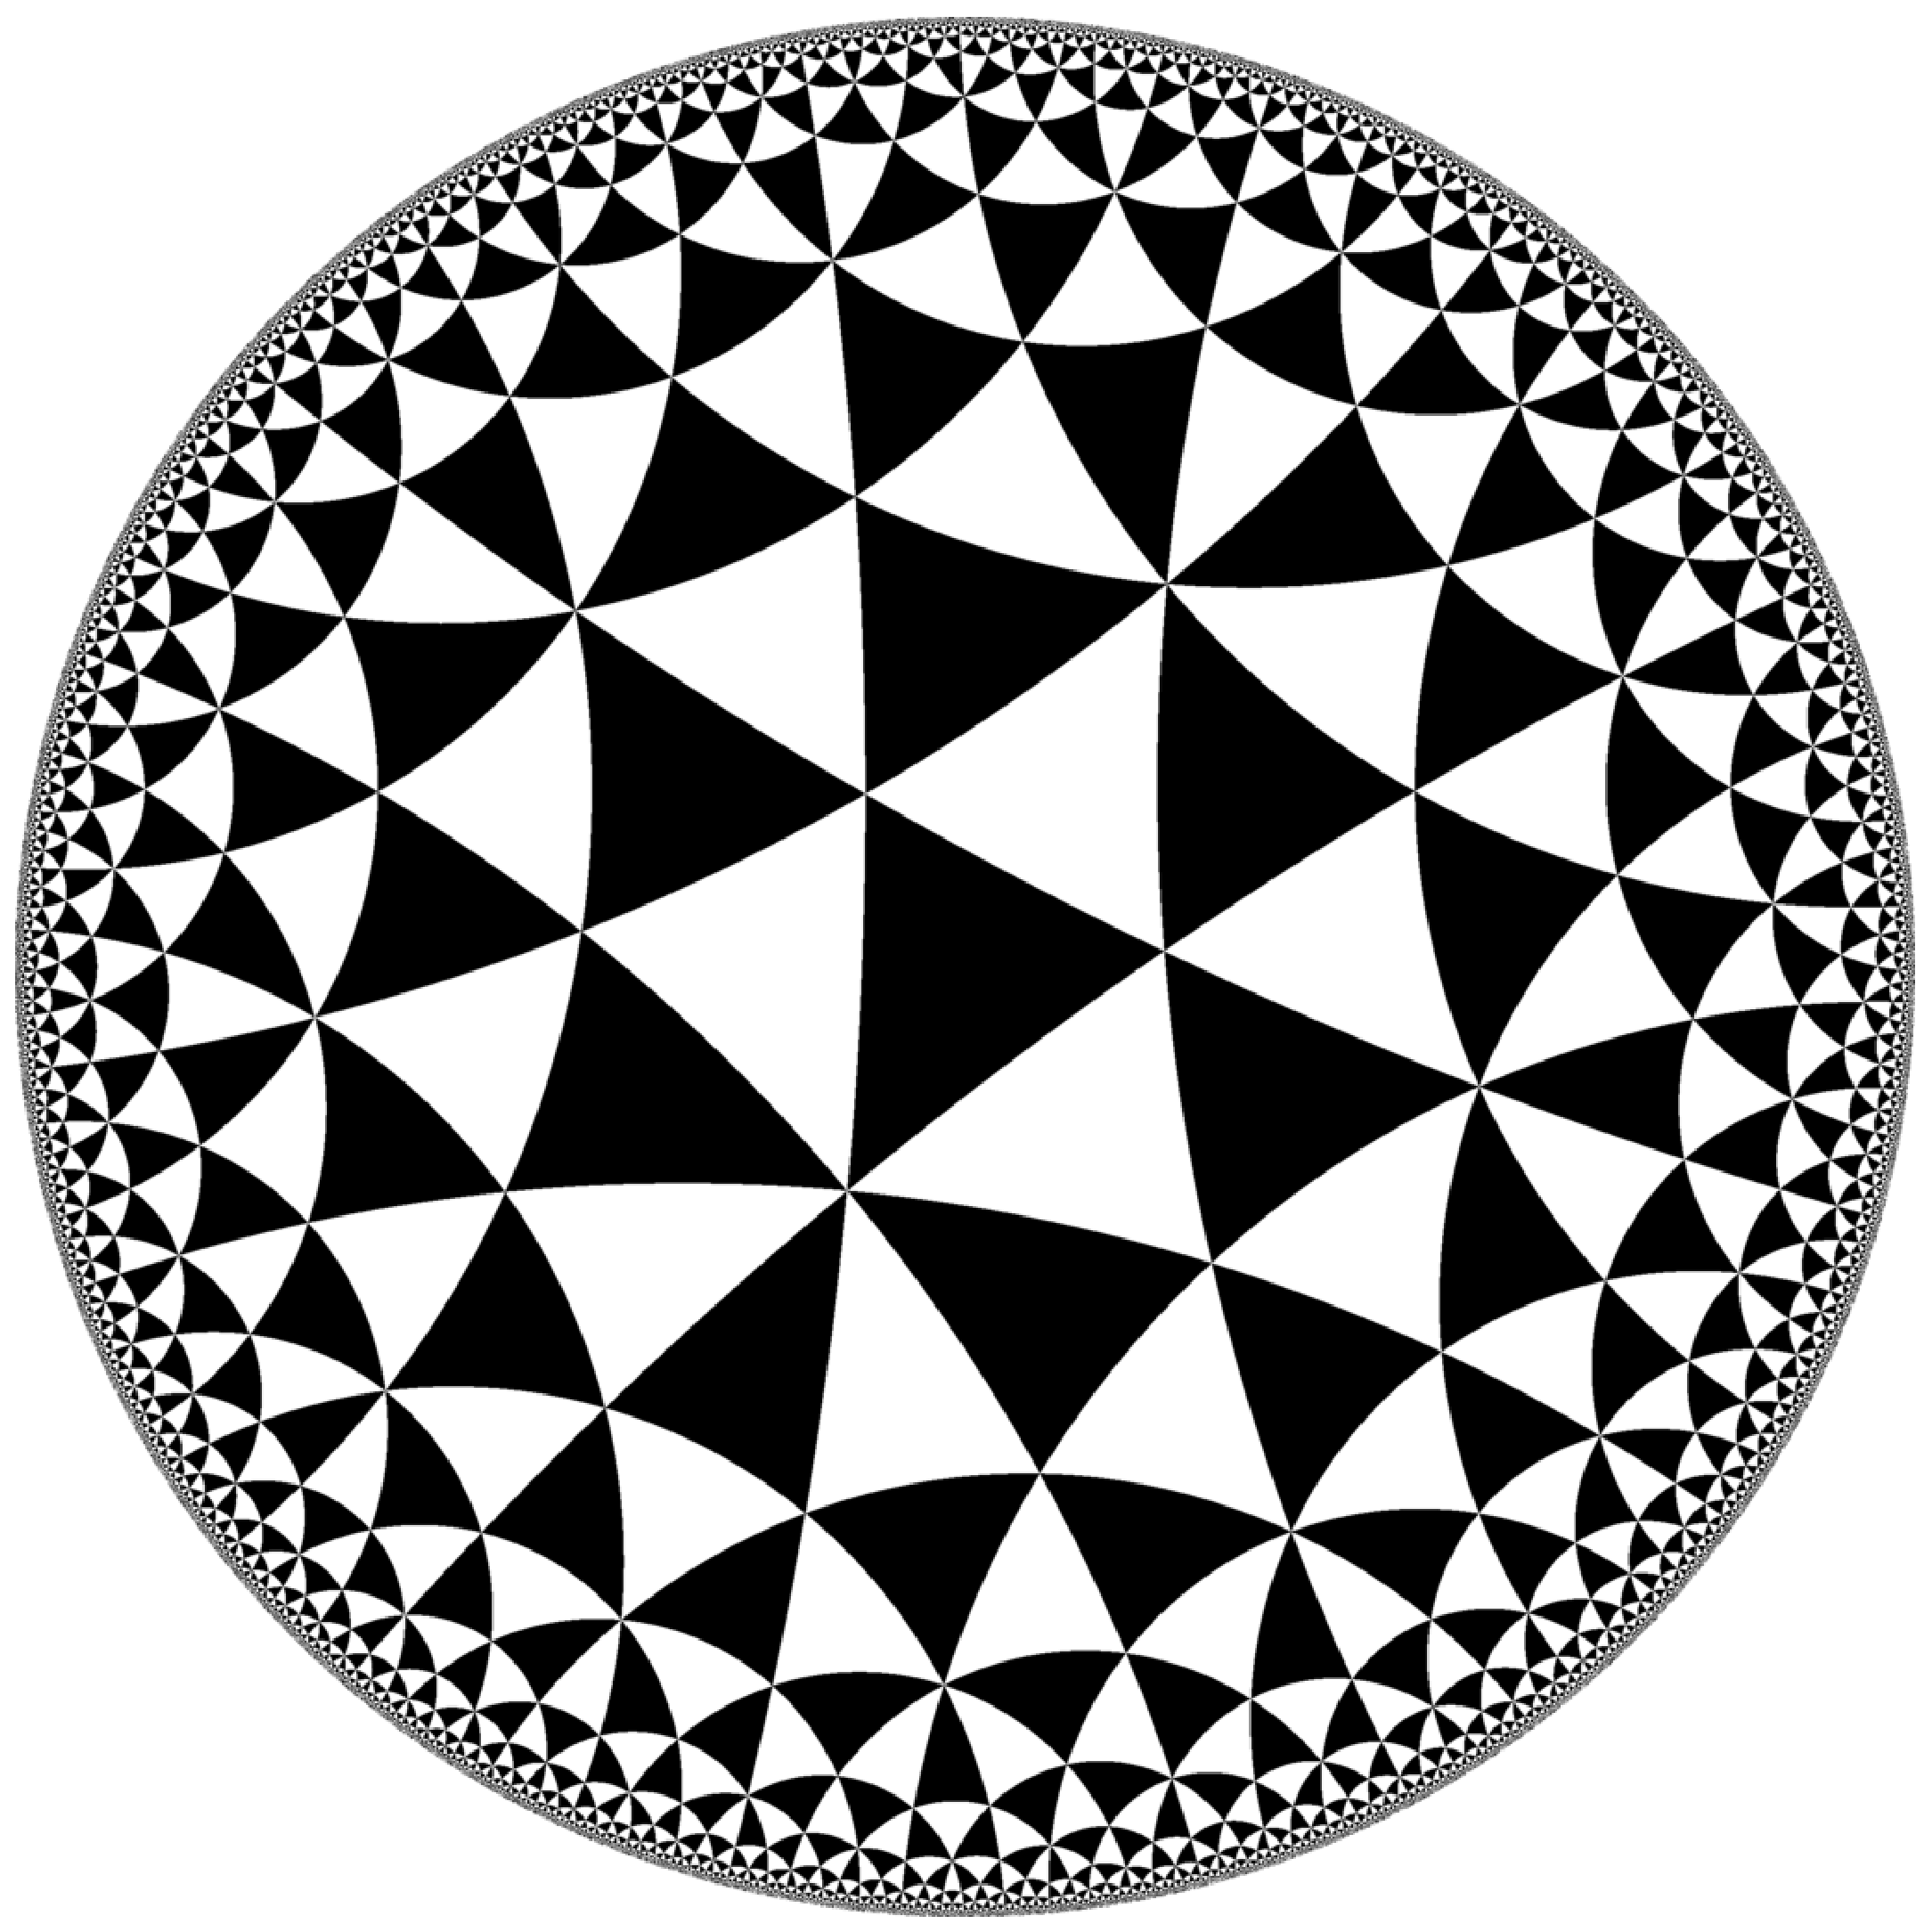
\includegraphics[scale=0.25]{pics/H2checkers_334}
\end{figure}

In this chapter, we use inversive geometry 
to construct the model of a hyperbolic plane --- a neutral plane that is not Euclidean.

Namely, we construct the so-called \index{conformal disc model}\emph{conformal disc model} of the hyperbolic plane.
This model was discovered by Eugenio Beltrami \cite{beltrami}; 
it is often called the {}\emph{Poincar\'e disc model}. 

The figure above shows the conformal disc model of the hyperbolic plane which is cut into congruent triangles with angles $\tfrac\pi3$, $\tfrac\pi3$, and~$\tfrac\pi4$.

\section{Conformal disc model}
\label{sec:conformal-model}

In this section, we give new names for certain objects in the Euclidean plane
which will represent lines, angle measures, and distances in the hyperbolic plane.

\parbf{Hyperbolic plane.}
Let us fix a circle on the Euclidean plane 
and call it \index{absolute}\emph{absolute}.
The set of points inside the absolute will be called the \index{hyperbolic!plane}\index{plane!hyperbolic plane}\emph{hyperbolic plane} (or \index{plane!h-plane}\index{h-plane}\emph{h-plane}).

Note that the points on the absolute do {}\emph{not} belong to the h-plane.
The points in the h-plane will be also called \index{h-point}\emph{h-points}.

Often we will assume that the absolute is a unit circle.



\parbf{Hyperbolic lines.}
The intersections of the h-plane with circlines perpendicular to the absolute are called {}\emph{hyperbolic lines} or \index{h-line}\emph{h-lines}.

\begin{wrapfigure}{o}{48mm}
\centering
\includegraphics{mppics/pic-190}
\end{wrapfigure}

By Corollary~\ref{cor:h-line}, there is a unique h-line that passes thru the given two distinct h-points $P$ and~$Q$.
This h-line will be denoted by~\index{62@$(PQ)_h$, $[PQ)_h$,$[PQ]_h$}$(PQ)_h$.

The arcs of hyperbolic lines will be called {}\emph{hyperbolic segments} or \index{h-segment}\emph{h-segments}.
An h-segment with endpoints $P$ and $Q$ will be denoted by~$[PQ]_h$.

The subset of an h-line on one side from a point will be called a {}\emph{hyperbolic half-line} (or \index{h-half-line}\emph{h-half-line}).
More precisely, an h-half-line is an intersection of the h-plane with an arc perpendicular to the absolute that has exactly one of its endpoints in the h-plane.
An h-half-line starting at $P$ and passing thru $Q$ will be denoted by~$[PQ)_h$.

If $\Gamma$ is the circline containing the h-line $(PQ)_h$, then the points of intersection of $\Gamma$ with the absolute are called 
\index{point!ideal point}\index{ideal!point}\emph{ideal points} of~$(PQ)_h$.
(Note that the ideal points of an h-line do not belong to the h-line.)

An ordered triple of h-points, say $(P,Q,R)$, will be called \emph{h-triangle $PQR$} and denoted by \index{21@$\triangle_h$}$\triangle_h P Q R$.

Let us point out, that so far an h-line $(PQ)_h$ is just a subset of the h-plane;
below we will introduce h-distance 
and later we will show that $(PQ)_h$ is a line for the h-distance in the sense of the Definition~\ref{def:line}. 

\begin{thm}{Exercise}\label{ex:ideal-line-unique}
Show that an h-line is uniquely determined by its ideal points.
\end{thm}

\begin{thm}{Exercise}\label{ex:1ideal-line-unique}
Show that an h-line is uniquely determined by one of its ideal points and one h-point on it.
\end{thm}

\begin{thm}{Exercise}\label{ex:line/h-line}
Show that the h-segment $[PQ]_h$ coincides with the Euclidean segment $[PQ]$
if and only if the line $(PQ)$ passes thru the center of the absolute.
\end{thm}

\parbf{Hyperbolic distance.}\label{h-dist}
Let $P$ and $Q$ be distinct h-points;
let $A$ and $B$ denote the ideal points of $(PQ)_h$.
Without loss of generality, we may assume that on the Euclidean circline containing the h-line $(PQ)_h$, the points $A,P,Q,B$ appear in the same order.

Consider the function 
$$\delta(P,Q)\df\frac{AQ\cdot PB}{AP\cdot QB}.$$
Note that the right-hand side is a cross-ratio;
by Theorem~\ref{lem:inverse-4-angle} it is invariant under inversion.
Set $\delta(P,P)=1$ for any h-point~$P$.
Let us define h-distance as the logarithm of $\delta$; that is,
$$PQ_h\df\ln[\delta(P,Q)].$$

The proof that $PQ_h$ is a metric on the h-plane will be given later.
For now, it is just a function that returns a real value $PQ_h$ for any pair of h-points $P$ and~$Q$.

\begin{thm}{Exercise}\label{ex:h-dist-eq}
Let $O$ be the center of the absolute and the h-points $O$, $X$, and $Y$ lie on one h-line in the same order.
Assume $OX\z=XY$.
Prove that $OX_h<XY_h$.
\end{thm}


\parbf{Hyperbolic angles.}\label{h-angle measure}
Consider three h-points $P$, $Q$, and $R$
such that $P\ne Q$ and $R\ne Q$.
The \index{hyperbolic!angle}\emph{hyperbolic angle $PQR$} (briefly $\angle_h PQR$)\index{11@$\angle_h$, $\measuredangle_h$} is an ordered pair of h-half-lines $[QP)_h$ and $[QR)_h$.

Let $[QX)$ and $[QY)$ be (Euclidean) half-lines 
that are tangent to $[QP]_h$ and $[QR]_h$ 
at~$Q$.
Then the \index{angle!measure!hyperbolic angle measure}\index{hyperbolic!angle measure}\emph{hyperbolic angle measure} (or \index{h-angle measure}\emph{h-angle measure}) of $\angle_h PQR$ is denoted by
$\measuredangle_h PQR$ and defined as
$\measuredangle XQY$.

\begin{thm}{Exercise}\label{ex:h-perp-unique}
Let $\ell$ be an h-line and $P$ be an h-point that does not lie on~$\ell$.
Show that there is a unique h-line thru $P$ and perpendicular to~$\ell$.
\end{thm}

\section{Plan of the proof}

We defined all the {}\emph{h-notions} needed in the formulation of the axioms \ref{def:birkhoff-axioms:0}--\ref{def:birkhoff-axioms:3} and h-\ref{def:birkhoff-axioms:4}.
It remains to show that all these axioms hold; 
this will be done by the end of this chapter.

Once we are done with the proofs, 
we get that the model provides an example of a neutral plane; 
in particular, Exercise~\ref{ex:h-perp-unique} can be proved the same way as Theorem~\ref{perp:ex+un}.

Most importantly we will prove the ``if''-part of Theorem~\ref{thm:consistent}.

Indeed, any statement in hyperbolic geometry can be restated in the Euclidean plane using the introduced h-notions.
Therefore, if the system of axioms \ref{def:birkhoff-axioms:0}--\ref{def:birkhoff-axioms:3}, and h-\ref{def:birkhoff-axioms:4} leads to a contradiction, then so does the system axioms \ref{def:birkhoff-axioms:0}--\ref{def:birkhoff-axioms:4}.

\section{Auxiliary statements}

One may compare the conformal model with a {}\emph{telescope} --- it makes it possible to {}\emph{see} the h-plane from the Euclidean plane.
Continuing this analogy further, we may say that the following lemma will be used to {}\emph{aim} the telescope at any particular point in the h-plane.

\begin{thm}{Lemma}\label{lem:P-->O} 
Consider an h-plane with a unit circle as the absolute.
Let $O$ be the center of the absolute and $P$ be another h-point.
Suppose that $P'$ denotes the inverse of $P$ across the absolute.

Then the circle $\Gamma$ with the center $P'$ and radius 
$\tfrac{\sqrt{1-OP^2}}{OP}$
is perpendicular to the absolute.
Moreover, $O$ is the inverse of $P$ across~$\Gamma$. 
\end{thm}

\begin{wrapfigure}[8]{o}{45mm}
\vskip-4mm
\centering
\includegraphics{mppics/pic-192}
\end{wrapfigure}

\parit{Proof.} 
Follows by Exercise~\ref{ex:centers-of-perp-circles}.
\qeds

Assume $\Gamma$ is a circline that is perpendicular to the absolute.
Consider the inversion $X\mapsto X'$ across $\Gamma$;
if $\Gamma$ is a line, set $X\mapsto X'$ to be the reflection across~$\Gamma$.

The following observation says that the map $X\mapsto X'$ respects all the notions introduced in the previous section.
Together with the lemma above, it implies that in any problem that is formulated entirely {}\emph{in h-terms} we can assume that a given h-point lies in the center of the absolute.

\begin{thm}{Main observation}\label{thm:main-observ}
The map $X\mapsto X'$ described above is a bijection from the h-plane to itself. 
Moreover, for any h-points $P$, $Q$, $R$ such that $P\ne Q$ and $Q\ne R$, the following conditions hold:
\begin{enumerate}[(a)]
\item\label{h-line-to-hline} The h-line $(PQ)_h$, h-half-line $[PQ)_h$, and h-segment $[PQ]_h$ are transformed into $(P'Q')_h$, $[P'Q')_h$, and $[P'Q']_h$ respectively.
\item\label{h-reflect} $\delta(P',Q')=\delta(P,Q)$ and $P'Q'_h=PQ_h$.
\item\label{h-angle-mes} 
$\measuredangle_h P'Q'R'\equiv-\measuredangle_h PQR$.
\end{enumerate}

\end{thm}

It is instructive to compare this observation with Proposition~\ref{prop:reflection}.

\parit{Proof.}
According to Theorem~\ref{thm:perp-inverse}, the map sends the absolute to itself. 
Note that the points on $\Gamma$ do not move, it follows that points inside of the absolute remain inside after the mapping.
Whence the $X\mapsto X'$ is a bijection from the h-plane to itself.


Part~\textit{(\ref{h-line-to-hline})} follows from \ref{thm:inverse-cline} and \ref{thm:angle-inversion}.

Part~\textit{(\ref{h-reflect})} follows from Theorem~\ref{lem:inverse-4-angle}.

Part~\textit{(\ref{h-angle-mes})} follows from Theorem~\ref{thm:angle-inversion}.
\qeds


\begin{thm}{Lemma}\label{lem:O-h-dist}
Assume that the absolute is a unit circle centered at~$O$.
Given an h-point $P$, set $x=OP$ and $y=OP_h$.
Then
\begin{align*}
y&=\ln\frac{1+x}{1-x}
&
&\text{and}
&
x&=\frac{e^y-1}{e^y+1}.
\end{align*}
 
\end{thm}

Observe that according to the lemma, $OP_h\to \infty$ as $OP\to 1$.
That is, if $P$ approaches absolute in the Euclidean sense, it escapes to infinity in the h-sense.

\begin{wrapfigure}[6]{o}{38mm}
\vskip-4mm
\centering
\includegraphics{mppics/pic-194}
\end{wrapfigure}

\parit{Proof.}
Note that the h-line $(OP)_h$ forms a diameter of the absolute.
If $A$ and $B$ are the ideal points as in the definition of the h-distance, then
\begin{align*}
OA&=OB=1,
\\ 
PA&=1+x,
\\
PB&=1-x.\end{align*}
In particular,
\begin{align*}
y&=\ln \frac{AP\cdot BO}{PB\cdot OA}=\ln\frac{1+x}{1-x}.
\end{align*}

Taking the exponential function of the left and the right-hand side and applying obvious algebra manipulations, we get that
$$x=\frac{e^y-1}{e^y+1}.$$
\qedsf


\begin{thm}{Lemma}\label{lem:h-tiangle=}
Assume the points $P$, $Q$, and $R$ appear on one h-line in the same order.
Then 
$$PQ_h+QR_h=PR_h.$$ 

\end{thm}

\parit{Proof.}
Note that
$$PQ_h+QR_h=PR_h$$
is equivalent to 
\[\delta(P,Q)\cdot\delta(Q,R)=\delta(P,R).\eqlbl{eq:deltaPQR}\]

Let $A$ and $B$ be the ideal points of~$(PQ)_h$. 
Without loss of generality, we can assume that the points $A$, $P$, $Q$, $R$, and $B$ appear in the same order on the circline containing $(PQ)_h$.
Then
\begin{align*}
\delta(P,Q)\cdot\delta(Q,R)
&=
\frac{AQ\cdot BP}{QB\cdot PA}\cdot\frac{AR\cdot BQ}{RB\cdot QA}=
\\
&=\frac{AR\cdot BP}{RB\cdot PA}=
\\
&=\delta(P,R).
\end{align*}
Hence \ref{eq:deltaPQR} follows.
\qeds

Let $P$ be an h-point and $\rho>0$.
The set of all h-points $Q$ such that $PQ_h=\rho$ is called an \index{h-circle}\emph{h-circle} with the center $P$ and the \index{h-radius}\emph{h-radius} $\rho$.

\begin{thm}{Lemma}\label{lem:h-circle=circle}
Any h-circle is a Euclidean circle that lies completely in the h-plane.

More precisely for any h-point $P$ and $\rho\ge 0$
there is a $\hat\rho\ge 0$ and a point $\hat P$ such that 
$$PQ_h= \rho
\quad 
\iff
\quad
\hat PQ= \hat\rho$$
for any h-point~$Q$.

Moreover, if $O$ is the center of the absolute, then 
\begin{enumerate}
\item $\hat O=O$ for any $\rho$ and
\item $\hat P\in (OP)$ for any $P\ne O$.
\end{enumerate}

\end{thm}

\parit{Proof.}
According to Lemma~\ref{lem:O-h-dist}, 
$OQ_h\z= \rho$ if and only if $$OQ= \hat\rho=\frac{e^\rho-1}{e^\rho+1}.$$
Therefore, the locus of h-points $Q$ such that $OQ_h= \rho$ is a Euclidean circle, 
denote it by $\Delta_\rho$.

\begin{wrapfigure}{o}{33mm}
\vskip-3mm
\centering
\includegraphics{mppics/pic-196}
\end{wrapfigure}

If $P\ne O$, then by Lemma~\ref{lem:P-->O} and the main observation (\ref{thm:main-observ})
there is an inversion that respects all h-notions and sends $O\mapsto P$.

Let $\Delta_\rho'$ be the inverse of $\Delta_\rho$.
Since the inversion preserves the h-distance,
$PQ_h=\rho$ if and only if $Q\z\in\Delta_\rho'$.

According to Theorem~\ref{thm:inverse-cline}, $\Delta_\rho'$ is a Euclidean circle.
Let $\hat P$ and $\hat\rho$ denote the Euclidean center and radius of $\Delta_\rho'$.

Finally, note that $\Delta_\rho'$ reflects to itself across $(OP)$;
that is, the center $\hat P$ lies on~$(OP)$.
\qeds

\begin{thm}{Exercise}\label{ex:h-circle=circle}
Describe a nondegenerate h-triangle $\triangle_hPQR$ that does not have an h-circumcircle;
that is, its vertices $P$, $Q$, and $R$ do not lie on an h-circle or h-line.
\end{thm}

\section[Axioms]{Axioms}
\subsection*{Axiom~\ref{def:birkhoff-axioms:0}}

Evidently, the h-plane contains at least two points.
Therefore, to show that Axiom~\ref{def:birkhoff-axioms:0} holds in the h-plane, we need to show that the h-distance defined in Section~\ref{sec:conformal-model} is a metric;
that is, the conditions \textit{(\ref{def:metric-space:a})}--\textit{(\ref{def:metric-space:d})} 
in Definition~\ref{def:metric-space} hold for h-distance.


The following claim says that the h-distance meets the conditions \textit{(\ref{def:metric-space:a})} 
and \textit{(\ref{def:metric-space:b})}.

\begin{thm}{Claim}
Given the h-points $P$ and $Q$, we have
$PQ_h\ge 0$
and $PQ_h=0$ if and only if $P=Q$.
\end{thm}


\parit{Proof.}
According to Lemma~\ref{lem:P-->O}
and the main observation (\ref{thm:main-observ}), 
we may assume that $Q$ is the center of the absolute.
In this case
$$
\delta(Q,P)=\frac{1+QP}{1-QP}\ge 1$$
and therefore
$$QP_h=\ln[\delta(Q,P)]\ge 0.$$
Moreover, the equalities hold if and only if $P=Q$.
\qeds

The following claim says that the h-distance meets Condition~\ref{def:metric-space}\textit{\ref{def:metric-space:c}}.

\begin{thm}{Claim}
For any h-points $P$ and $Q$, we have
$PQ_h=QP_h$.
\end{thm}

\parit{Proof.}
Let $A$ and $B$ be ideal points of $(PQ)_h$ and
$A,P,Q,B$ appear on the circline containing $(PQ)_h$ in the same order.

{

\begin{wrapfigure}{o}{33mm}
\vskip-5mm
\centering
\includegraphics{mppics/pic-198}
\end{wrapfigure}

Then
\begin{align*}
PQ_h
&=\ln\frac{AQ\cdot BP}{QB\cdot PA}
=
\\
&=\ln\frac{BP\cdot AQ}{PA\cdot QB}=
\\
&=QP_h.
\end{align*}
\qedsf

}

The following claim shows, in particular, that
the triangle inequality 
(which is condition \ref{def:metric-space}\textit{\ref{def:metric-space:d}})
holds for $h$-distance.

\begin{thm}{Claim}\label{clm:h-dist+trig-inq}
Given a triple of h-points $P$, $Q$, and $R$,
we have
\[PQ_h+QR_h\ge PR_h.\]
Moreover, the equality holds if and only if $P$, $Q$, and $R$ lie on one h-line in the same order.
\end{thm}

\parit{Proof.}
Without loss of generality, we may assume that $P$ is the center of the absolute
and 
$0<QR_h\le PQ_h$.

Let $\Delta$ be the h-circle with the center $Q$ and h-radius $QR_h$.
Choose points $S$ and $T$ on the intersection of $(PQ)$ with~$\Delta$ so that $P$, $S$, $Q$, and $T$ appear on the h-line in the same order.
The latter is possible by Lemma~\ref{lem:h-tiangle=}, since $QS_h\z=QT_h\z=QR_h\z\le PQ_h$.

{

\begin{wrapfigure}{o}{35mm}
\vskip-0mm
\centering
\includegraphics{mppics/pic-200}
\end{wrapfigure}

According to Lemma~\ref{lem:h-circle=circle}, $\Delta$ is a Euclidean circle;
let $\hat Q$ be its Euclidean center.

Note that $\hat QS\z=\hat QT\z=\hat QR$.
By the Euclidean triangle inequality,
$$PT
=
P\hat Q+\hat Q R
\ge 
PR,
\eqlbl{RT>RQ}$$
and the equality holds if and only if $T=R$. 

By Lemma~\ref{lem:O-h-dist},
\begin{align*}
PT_h&=\ln\frac{1+PT}{1-PT},\\
PR_h&=\ln\frac{1+PR}{1-PR}.
\end{align*}
Note that the function $x\mapsto\ln\frac{1+x}{1-x}$ is increasing for $0\le x<1$.
Therefore, \ref{RT>RQ} implies
$$PT_h\ge PR_h;$$
moreover, the equality holds if and only if $T\z=R$.

}

Finally, applying Lemma~\ref{lem:h-tiangle=} again, 
we get that
$$PT_h=PQ_h+QR_h.$$
Hence the claim follows.
\qeds

\subsection*{Axiom~\ref{def:birkhoff-axioms:1}}

Note that once the following claim is proved,
Axiom~\ref{def:birkhoff-axioms:1} 
follows from Corollary~\ref{cor:h-line}.

\begin{thm}{Claim}
A subset of the h-plane is an h-line if and only if it forms a line for the h-distance in the sense of Definition~\ref{def:line}.
\end{thm}

\parit{Proof.}
Let $\ell$ be an h-line.
Applying the main observation (\ref{thm:main-observ}) we can assume that $\ell$ contains the center of the absolute.
In this case, $\ell$ is an intersection of a diameter of the absolute and the h-plane.
Let $A$ and $B$ be the endpoints of the diameter.

\begin{wrapfigure}{o}{29mm}
\vskip-5mm
\centering
\includegraphics{mppics/pic-201}
\end{wrapfigure}

Consider the map $\iota\:\ell\to \mathbb{R}$ defined as
$$\iota(X)=\ln \frac{AX}{XB}.$$
Note that $\iota\:\ell\to \mathbb{R}$ is a bijection.

Further, if $X,Y\in \ell$ and the points $A$, $X$, $Y$, and $B$ appear on $[AB]$ in the same order, then
\[\iota(Y)-\iota(X)=\ln \frac{AY}{YB}-\ln \frac{AX}{XB}=\ln \frac{AY\cdot BX}{YB\cdot XB}=XY_h.\]

We proved that any h-line is a line for h-distance.
The converse follows from Claim~\ref{clm:h-dist+trig-inq}.
\qeds


\subsection*{Axiom~\ref{def:birkhoff-axioms:2}}

Note that the first part of Axiom~\ref{def:birkhoff-axioms:2} follows directly from the definition of the h-angle measure (defined in Section~\ref{sec:conformal-model}).
It remains to show that $\measuredangle_h$ satisfies the conditions \ref{def:birkhoff-axioms:2a}, \ref{def:birkhoff-axioms:2b}, and \ref{def:birkhoff-axioms:2c} (see Section~\ref{sec:axioms}).

The following two claims say that
$\measuredangle_h$ satisfies
 \ref{def:birkhoff-axioms:2a} and \ref{def:birkhoff-axioms:2b}.

\begin{thm}{Claim}\label{clm:h2a}
Given an h-half-line $[O P)_h$ and $\alpha\in(-\pi,\pi]$, there is a unique h-half-line $[O Q)_h$ such that $\measuredangle_h P O Q= \alpha$.
\end{thm}

\begin{thm}{Claim}\label{clm:h2b}
For any h-points $P$, $Q$, and $R$ distinct from an h-point $O$, we have
$$\measuredangle_h P O Q+\measuredangle_h Q O R
\equiv\measuredangle_h P O R.$$

\end{thm}

\parit{Proof of \ref{clm:h2a} and \ref{clm:h2b}.}
Applying the main observation, 
we may assume that $O$ is the center of the absolute.
In this case, for any h-point $P\z\ne O$, the h-half-line
$[OP)_h$ is the intersection of the Euclidean half-line $[OP)$ with h-plane.
Hence \ref{clm:h2a} and \ref{clm:h2b} 
follow from the axioms \ref{def:birkhoff-axioms:2a} and \ref{def:birkhoff-axioms:2b} of the Euclidean plane.
\qeds

The following claim says that
$\measuredangle_h$ satisfies
 \ref{def:birkhoff-axioms:2c}.

\begin{thm}{Claim}\label{clm:h2c}
The function 
$$\measuredangle_h\:(P,Q,R)\mapsto\measuredangle_h P Q R$$
is continuous at any triple of points $(P,Q,R)$
such that $Q\ne P$, $Q\ne R$, and $\measuredangle_h P Q R\ne\pi$.
\end{thm}

\parit{Proof.}
Suppose that $O$ denotes the center of the absolute.
We can assume that $Q$ is distinct from~$O$;
the latter follows from the main observation.

\begin{wrapfigure}{o}{45mm}
\vskip-4mm
\centering
\includegraphics{mppics/pic-199}
\end{wrapfigure}

Let $Z$ be the inverse of $Q$ across the absolute;
denote by $\Gamma$ the circle with the center at~$Z$ that is perpendicular to the absolute.
According to Lemma~\ref{lem:P-->O},
point $O$ is the inverse of $Q$ across~$\Gamma$.

Let $P'$ and $R'$ be the inversions across $\Gamma$ of the points $P$ and $R$ respectively.
Note that the point $P'$ is completely determined by $Q$ and $P$.
Moreover, the map $(Q,P)\mapsto P'$ is continuous at any pair of h-points $(Q,P)$ such that $Q\ne O$.
The same is true for the map $(Q,R)\mapsto R'$.

According to the main observation 
$$\measuredangle_h P Q R\equiv -\measuredangle_h P' O R'.$$
Since $\measuredangle_h P' O R'=\measuredangle P' O R'$ and 
the maps $(Q,P)\mapsto P'$, $(Q,R)\mapsto R'$ are continuous,
the claim follows from the corresponding axiom of the Euclidean plane.
\qeds

\subsection*{Axiom~\ref{def:birkhoff-axioms:3}}

The following claim says that Axiom~\ref{def:birkhoff-axioms:3} holds in the h-plane.

\begin{thm}{Claim}
In the h-plane, we have
$\triangle_h P Q R 
\cong
\triangle_h P' Q' R'$
if and only if 
\begin{align*}
Q' P'_h&=Q P_h, & Q' R'_h&= Q R_h &&\text{and}
&\measuredangle_h P' Q' R'&=\pm\measuredangle P Q R.
\end{align*}
 
\end{thm}

\parit{Proof.}
Applying the main observation, 
we can assume that $Q$ and $Q'$ coincide with the center of the absolute; in particular, $Q=Q'$.
In this case, 
$$\measuredangle P' Q R'=\measuredangle_h P' Q R'=\pm\measuredangle_h P Q R=\pm\measuredangle P Q R.$$
Since 
$$Q P_h=Q P'_h\quad \text{and}\quad Q R_h=Q R'_h,$$
Lemma~\ref{lem:O-h-dist} implies that the same holds for the Euclidean distances;
that is,
$$Q P=Q P'
\quad
\text{and}
\quad
Q R=Q R'.$$
By SAS,
there is a motion of the Euclidean plane that sends
$Q$ to itself,
$P$ to $P'$, 
and $R$ to $R'$.

Note that the center of the absolute is fixed by the corresponding motion.
It follows that this motion gives also a motion of the h-plane;
in particular, the h-triangles 
$\triangle_h P Q R$ and $\triangle_h P' Q R'$ are h-congruent.
\qeds

\subsection*{Axiom h-$\!$\ref{def:birkhoff-axioms:4}}

Finally, we need to check that the Axiom~h-$\!$\ref{def:birkhoff-axioms:4} in Section~\ref{sec:unprovable} holds;
that is, we need to prove the following claim.

{

\begin{wrapfigure}{o}{31mm}
\vskip-4mm
\centering
\includegraphics{mppics/pic-202}
\end{wrapfigure}

\begin{thm}{Claim}
For any h-line $\ell$ and any h-point $P\notin\ell$ there are at least two h-lines that pass thru $P$ 
and have no points of intersection with~$\ell$.
\end{thm}

\parit{Instead of proof.}
Applying the main observation we can assume that $P$ is the center of the absolute.

The remaining part of the proof can be guessed from the picture.
\qeds

}

\begin{thm}{Exercise}\label{ex:3-h-lines}
\begin{enumerate}[(a)]
\item Show that in the h-plane there are 3 mutually parallel h-lines 
such that any pair of these three lines lies on one side of the remaining h-line.
\item Draw three h-lines $\ell$, $m$, and $n$ such that $\ell\parallel m$, $m\parallel n$, but $\ell\nparallel n$.
Conclude that the parallelness is not an equivalence relation for h-lines.
\end{enumerate}
\end{thm}
 
\section{Hyperbolic trigonometry}
\label{sec:hyp-trig}


In this section, we give formulas for h-distance using \index{hyperbolic!functions}\emph{hyperbolic functions}.
One of these formulas will be used in the proof of the hyperbolic Pythagorean theorem (\ref{thm:pyth-h-poincare}).

Recall that $\cosh$, $\sinh$, and $\tanh$ denote \index{ch@$\cosh$}\index{hyperbolic!cosine}\emph{hyperbolic cosine}, \index{sh@$\sinh$}\index{hyperbolic!sine}\emph{hyperbolic sine}, and \index{th@$\tanh$}\index{hyperbolic!tangent}\emph{hyperbolic tangent}\label{hyperbolic tangent};
that is, the functions defined by
\[\cosh x\df \tfrac{e^x+e^{-x}}2,
 \quad
 \sinh x\df \tfrac{e^x-e^{-x}}2,
\]
\[\tanh x\df \tfrac{\sinh x}{\cosh x}.
\]

These hyperbolic functions are analogous to sine and cosine and tangent. 

\begin{thm}{Exercise}\label{ex:hyp-fun}
Prove the following identities:
\[\cosh' x=\sinh x;\quad \sinh'x=\cosh x;\quad (\cosh x)^2-(\sinh x)^2=1.\]
\end{thm}

\begin{thm}{Double-argument identities}\label{double-argument}
The identities
\begin{align*}
\cosh (2\cdot x)&=(\cosh x)^2+(\sinh x)^2 
&&\text{and}&
\sinh (2\cdot x)&=2\cdot\sinh x\cdot \cosh x
\end{align*}
hold for any real value $x$.
\end{thm}

\parit{Proof.}
\begin{align*}
(\sinh x)^2+(\cosh x)^2
&=(\tfrac{e^x-e^{-x}}2)^2+(\tfrac{e^x+e^{-x}}2)^2=
\\
&=\tfrac{e^{2\cdot x}+e^{-2\cdot x}}2=
\\
&=\cosh (2\cdot x);
\\
2\cdot\sinh x\cdot \cosh x
&=2\cdot(\tfrac{e^x-e^{-x}}2)\cdot(\tfrac{e^x+e^{-x}}2)=
\\
&=\tfrac{e^{2\cdot x}-e^{-2\cdot x}}2=
\\
&=\sinh (2\cdot x).
\end{align*}
\qedsf

\begin{thm}{Advanced exercise}\label{ex:cosh}
Let $P$ and $Q$ be two h-points distinct from the center of absolute.
Denote by $P'$ and $Q'$ the inverses of $P$ and $Q$ across the absolute.

\begin{wrapfigure}[20]{r}{40mm}
\centering
\includegraphics{mppics/pic-204}
\end{wrapfigure}

Show that 
\medskip
\begin{enumerate}[(a)]
\item\label{ex:cosh/2} 
$\displaystyle{\cosh[\tfrac12\cdot PQ_h]=\sqrt{\frac{PQ'\cdot P'Q}{PP'\cdot QQ'}};}$
\medskip
\item\label{ex:coshsinh} 
$\displaystyle{\sinh[\tfrac12\cdot PQ_h]=\sqrt{\frac{PQ\cdot P'Q'}{PP'\cdot QQ'}};}$
\medskip
\item\label{ex:coshtanh} 
$\displaystyle{\tanh[\tfrac12\cdot PQ_h]=\sqrt{\frac{PQ\cdot P'Q'}{PQ'\cdot P'Q}};}$
\medskip
\item\label{ex:coshcosh} 
$\displaystyle{\cosh PQ_h=\frac{PQ\cdot P'Q'+PQ'\cdot P'Q}{PP'\cdot QQ'}.}$
\end{enumerate}

\end{thm}

\chapter{Geometry of the h-plane}\label{chap:h-plane}

In this chapter, we study the geometry of the plane described by the conformal disc model.
For briefness, this plane will be called the {}\emph{h-plane}.

We can work with this model directly from inside of the Euclidean plane. 
We may also use the axioms of neutral geometry since they all hold in the h-plane; the latter proved in the previous chapter.

\section{Angle of parallelism}

Let $P$ be a point off an h-line~$\ell$. 
Drop a perpendicular $(PQ)_h$ from $P$ to $\ell$;
let $Q$ be its foot point.
Let $\phi$ be the smallest value such that the h-line $(PZ)_h$ with $|\measuredangle_h Q P Z|=\phi$ does not intersect~$\ell$.

The value $\phi$ is called the \index{angle!angle of parallelism}\emph{angle of parallelism} of $P$ to~$\ell$.
Clearly, $\phi$ depends only on the h-distance $s=PQ_h$.
Further, $\phi(s)\to \pi/2$ as $s\to 0$, 
and $\phi(s)\to0$ as $s\to\infty$.
(In Euclidean geometry, the angle of parallelism is identically equal to~$\pi/2$.)

\begin{wrapfigure}{o}{34mm}
\vskip-6mm
\centering
\includegraphics{mppics/pic-206}
\end{wrapfigure}

If $\ell$, $P$, and $Z$ are as above, then the h-line $m=(PZ)_h$ is called \index{asymptotically parallel lines}\emph{asymptotically parallel} to~$\ell$.
In other words, two h-lines are asymptotically parallel if they share one ideal point.
(In hyperbolic geometry, the term {}\emph{parallel lines} is often used for \index{asymptotically parallel lines}\emph{asymptotically parallel lines}; we do not follow this convention.)

Given $P\not\in\ell$, there are exactly two asymptotically parallel lines thru $P$ to $\ell$; 
the remaining parallel lines are called \index{parallel lines!ultra parallel lines}\emph{ultra parallel}.


On the diagram, the two solid h-lines passing thru $P$ are asymptotically parallel to~$\ell$;
the dashed h-line is ultra parallel to~$\ell$.


\begin{thm}{Exercise}\label{ex:ultra-parallel}
Show that two distinct h-lines $\ell$ and $m$ are ultraparallel if and only if they have a \emph{common perpendicular};
that is, there is an $h$-line $n$ such that $n\perp \ell$ and $n\perp m$.
\end{thm}






\begin{thm}{Proposition}\label{prop:angle-parallelism}
Let $Q$ be the foot point of $P$ on h-line~$\ell$.
Then
\[PQ_h=\tfrac12\cdot\ln \frac{1+\cos\phi}{1-\cos\phi},\]
where $\phi$ is the angle of parallelism of $P$ to~$\ell$.

In particular, if $P\notin\ell$ and $\beta\z=|\measuredangle_h XPY|$ for some points $X,Y\in\ell$, then 
\[PQ_h<\tfrac12\cdot\ln \frac{1+\cos\tfrac\beta2}{1-\cos\tfrac\beta2}.\]

\end{thm}

\begin{wrapfigure}{o}{50mm}
\vskip-6mm
\centering
\includegraphics{mppics/pic-208}
\end{wrapfigure}


\parit{Proof.} Applying a motion of the h-plane if necessary,
we may assume $P$ is the center of the absolute.
Then the h-lines thru $P$ are the intersections of Euclidean lines with the h-plane.

Let $A$ and $B$ denote the ideal points of~$\ell$.
Without loss of generality, we may assume that $\angle APB$ 
is positive.
In this case, 
$$\phi=\measuredangle QPB=\measuredangle APQ=\tfrac12 \cdot\measuredangle APB.$$

Let $Z$ be the center of the circle $\Gamma$ containing the h-line~$\ell$.
Set $X$ to be the point of intersection of the Euclidean segment $[AB]$ and the line~$(PQ)$.

Note that, $PX=\cos\phi$.
Therefore, by Lemma~\ref{lem:O-h-dist},
$$PX_h=\ln \tfrac{1+\cos\phi}{1-\cos\phi}.$$

Note that both angles $PBZ$ and $BXZ$ are right.
Since the angle $PZB$ is shared, $\triangle ZBX\sim \triangle ZPB$.
In particular, 
$$ZX\cdot ZP=ZB^2;$$
that is, $X$ is the inverse of $P$ in~$\Gamma$.

The inversion in $\Gamma$ is the reflection of the h-plane across~$\ell$. 
Therefore
\begin{align*}
PQ_h&=QX_h=
\\
&=\tfrac12\cdot PX_h=
\\
&=\tfrac12\cdot\ln \tfrac{1+\cos\phi}{1-\cos\phi}.
\end{align*}

\begin{wrapfigure}{o}{46mm}
\vskip-0mm
\centering
\includegraphics{mppics/pic-209}
\end{wrapfigure}

The last statement follows since $\phi\z>\tfrac\beta2$ and the function 
\[\phi\mapsto  \tfrac12\cdot\ln \tfrac{1+\cos\phi}{1-\cos\phi}\] 
is decreasing in the interval $(0,\tfrac\pi2]$.
\qeds

\begin{thm}{Exercise}\label{ex:small-angle}
Let $ABC$ be an equilateral h-triangle with side $100$.
Show that 
\[|\measuredangle_h ABC|<\frac1{10\,000\,000\,000}.\]
\end{thm}

\section{Inradius of h-triangle}

\begin{thm}{Theorem}\label{thm:h-inradius}
The inradius of any h-triangle 
is less than $\tfrac12\cdot\ln3$.
\end{thm}

\parit{Proof.}
Let $I$ and $r$ be the h-incenter and h-inradius of $\triangle_hXYZ$.

Note that the h-angles 
$XIY$, 
$YIZ$ and 
$ZIX$
have the same sign.
Without loss of generality, we can assume that all of them are positive
and therefore
\[\measuredangle_hXIY+ 
\measuredangle_hYIZ+ 
\measuredangle_hZIX=2\cdot\pi
\]

{

\begin{wrapfigure}{o}{44mm}
\centering
\includegraphics{mppics/pic-210}
\end{wrapfigure}

We can assume that
$\measuredangle_hXIY\ge\tfrac23\cdot\pi$;
if not relabel $X$, $Y$, and $Z$. 

Since $r$ is the h-distance from $I$ to $(XY)_h$,
Proposition~\ref{prop:angle-parallelism} implies that
\begin{align*}r&<\tfrac12\cdot\ln \tfrac{1+\cos\frac\pi3}{1-\cos\frac\pi3}=
\\
&=\tfrac12\cdot\ln\frac{1+\tfrac12}{1-\tfrac12}=
\\
&=\tfrac12\cdot\ln 3.
\end{align*}
\qedsf

}

\begin{thm}{Exercise}\label{ex:side-sup}
Let $\square_h ABCD$ be a quadrangle in the h-plane 
such that the h-angles at $A$, $B$, and $C$ are right and $AB_h=BC_h$.
Find the optimal upper bound for~$AB_h$.
\end{thm}


\section{Circles, horocycles, and equidistants}

Note that according to Lemma~\ref{lem:h-circle=circle},
any h-circle is a Euclidean circle that lies completely in the h-plane.
Further, any h-line is an intersection of the h-plane with the circle 
perpendicular to the absolute.

In this section, we will describe the 
h-geometric meaning of the intersections 
of the other circles with the h-plane.

You will see that all these intersections have a {}\emph{perfectly round shape} in the h-plane.

One may think of these curves as trajectories of a car with a fixed position of the steering wheel.
In the Euclidean plane, 
this way you either run along a circle or a line.

In the hyperbolic plane, the picture is different.
If you turn the steering wheel to the far right, you will run along a circle.
If you turn it less, at a certain position of the wheel, you will never come back to the same point, but the path will be different from the line.
If you turn the wheel further a bit, you start to run along a path that stays at some fixed distance from an h-line.

\parbf{Equidistants of h-lines.}
Consider the h-plane with the absolute~$\Omega$.
Assume a circle $\Gamma$ intersects $\Omega$ in two distinct points, $A$ and~$B$. 
Suppose that $g$ denotes the intersection of $\Gamma$ with the h-plane.

\begin{wrapfigure}{o}{46mm}
\vskip-0mm
\centering
\includegraphics{mppics/pic-212}
\end{wrapfigure}

Let us draw an h-line $m$ with the ideal points $A$ and~$B$.
According to Exercise~\ref{ex:ideal-line-unique}, $m$ is uniquely defined.

Consider any h-line $\ell$ perpendicular to~$m$;
let $\Delta$ be the circle containing~$\ell$.

Note that $\Delta\perp \Gamma$.
Indeed,
according to Corollary~\ref{cor:perp-inverse-clines}, $m$ and $\Omega$ invert to themselves in~$\Delta$.
It follows that $A$ is the inverse of $B$ in~$\Delta$.
Finally, by Corollary~\ref{cor:perp-inverse}, we get that $\Delta\perp \Gamma$.

Therefore, inversion in $\Delta$ sends both $m$ and $g$ to themselves.
For any two points $P',P\in g$ there is a choice of $\ell$ and $\Delta$ as above such that
$P'$ is the inverse of $P$ in $\Delta$.
By the main observation (\ref{thm:main-observ}) the inversion in $\Delta$ is a motion of the h-plane. Therefore, all points of $g$ lie at the same distance from~$m$.

In other words, $g$ is the set of points that lie at a fixed h-distance and on the same side of~$m$.



Such a curve $g$ is called 
\index{equidistant}\emph{equidistant} to h-line~$m$.
In Euclidean geometry, the equidistant from a line is a line;
apparently, in hyperbolic geometry, the picture is different.

\parbf{Horocycles.}
If the circle $\Gamma$ touches the absolute from inside at one point $A$, then the complement $h=\Gamma\backslash\{A\}$ lies in the h-plane.
This set is called a \index{horocycle}\emph{horocycle}.
It also has a perfectly round shape in the sense described above.


\begin{wrapfigure}{r}{33mm}
\vskip-6mm
\centering
\includegraphics{mppics/pic-214}
\end{wrapfigure}

The shape of a horocycle is between shapes of circles and equidistants to h-lines.
A horocycle might be considered as a limit of circles 
thru a fixed point
with the centers running to infinity along a line.
The same horocycle is a limit of equidistants thru a fixed point to sequence of h-lines that runs to infinity.

Since any three points lie on a circline, we have that any nondegenerate h-triangle is inscribed in an h-circle, horocycle, or equidistant.

\begin{thm}{Exercise}\label{ex:right-trig-horocycle}
Find the leg of an isosceles right h-triangle inscribed in a horocycle.
\end{thm}




\section{Hyperbolic triangles}

\begin{thm}{Theorem}\label{thm:3sum-h}
Any nondegenerate hyperbolic triangle has a positive defect.
\end{thm}


\begin{wrapfigure}{o}{35mm}
\centering
\includegraphics{mppics/pic-216}
\end{wrapfigure}

\parit{Proof.}
Fix an h-triangle $ABC$.
According to Theorem~\ref{thm:3sum-a},
$$\defect(\triangle_hABC)\ge 0.\eqlbl{eq:defect<0}$$
It remains to show that in the case of equality, $\triangle_hABC$ degenerates.

Without loss of generality, we may assume that $A$ is the center of the absolute;
in this case, 
$\measuredangle_h CAB\z=\measuredangle CAB$.
Yet we may assume that 
$$\measuredangle_h CAB,
\quad 
\measuredangle_h ABC,
\quad
\measuredangle_h BCA,
\quad
\measuredangle ABC,
\quad
\measuredangle BCA\ge 0.$$

Let $D$ be an arbitrary point in $[CB]_h$ distinct from $B$ and~$C$.
From Proposition~\ref{prop:arc(angle=tan)}, we have
$$\measuredangle ABC-\measuredangle_h ABC \equiv 
\pi-\measuredangle CDB
\equiv \measuredangle BCA-\measuredangle_h BCA.$$

From Exercise~\ref{ex:|3sum|}, we get that
$$\defect(\triangle_hABC)=2\cdot(\pi-\measuredangle CDB).$$
Therefore, if we have equality in \ref{eq:defect<0}, then $\measuredangle CDB=\pi$.
In particular, the h-segment $[BC]_h$ coincides with the Euclidean segment~$[BC]$.
By Exercise~\ref{ex:line/h-line},
the latter can happen only if the h-line $(BC)_h$ passes thru the center of the absolute ($A$);
that is, if $\triangle_hABC$ degenerates.
\qeds

The following theorem states, in particular, that nondegenerate hyperbolic triangles are congruent if their corresponding angles are equal.
In particular, in hyperbolic geometry, similar triangles have to be congruent.

{\sloppy 
\begin{thm}{AAA congruence condition}\label{thm:AAA}\index{AAA congruence condition}
Two nondegenerate h-triangles
 $ABC$ and $A'B'C'$
 are congruent if
$\measuredangle_hABC\z=\pm\measuredangle_hA'B'C'$,
$\measuredangle_hBCA\z=\pm\measuredangle_hB'C'A'$
and 
$\measuredangle_hCAB=\pm\measuredangle_hC'A'B'$.
\end{thm}

}

\parit{Proof.}
Note that if $AB_h=A'B'_h$, then the theorem follows from ASA.

\begin{wrapfigure}{o}{32mm}
\centering
\includegraphics{mppics/pic-218}
\end{wrapfigure}

Assume the contrary. 
Without loss of generality, we may assume that $AB_h<A'B'_h$.
Therefore, we can choose the point $B''\in [A'B']_h$ such that $A'B''_h=AB_h$.

Choose an h-half-line $[B''X)$ so that 
\[\measuredangle_h A'B''X=\measuredangle_h A'B'C'.\]
According to Exercise~\ref{ex:parallel-abs}, $(B''X)_h\parallel(B'C')_h$.

By Pasch's theorem (\ref{thm:pasch}), $(B''X)_h$ intersects~$[A'C']_h$.
Suppose that $C''$ denotes the point of intersection.

According to ASA, $\triangle_h ABC\cong\triangle_h A'B''C''$;
in particular, 
$$\defect(\triangle_h ABC)=\defect(\triangle_h A'B''C'').
\eqlbl{eq:defect=defect}$$

Applying Exercise~\ref{ex:defect} twice, we get that
$$\begin{aligned}
\defect(\triangle_h A'B'C')
&=
\defect(\triangle_h A'B''C'')
+
\\
&+\defect(\triangle_h B''C''C')+\defect(\triangle_h B''C'B').
\end{aligned}
\eqlbl{eq:defect+defect}$$
By Theorem~\ref{thm:3sum-h}, all the defects have to be positive.
Therefore
$$\defect(\triangle_h A'B'C')
>\defect(\triangle_h ABC).$$
On the other hand,
$$\begin{aligned}
\defect(\triangle_h A'B'C')
&= |\measuredangle_hA'B'C'|+|\measuredangle_hB'C'A'|+|\measuredangle_hC'A'B'|=
\\
&=|\measuredangle_hABC|+|\measuredangle_hBCA|+|\measuredangle_hCAB|=
\\
&=\defect(\triangle_h ABC)
 \end{aligned}$$
--- a contradiction.
\qeds

Recall that a bijection from an h-plane to itself is called \index{angle-preserving transformation}\emph{angle-preserving} if 
\[\measuredangle_h ABC= \measuredangle_h A'B'C'\]
for any $\triangle_h ABC$ and its image $\triangle_h A'B'C'$.

\begin{thm}{Exercise}\label{ex:angle-preserving-hyp}
Show that any angle-preserving transformation of the h-plane is a motion.
\end{thm}

\section{Conformal interpretation}

Let us give another interpretation of the h-distance.

\begin{thm}{Lemma}\label{lem:conformal}
Consider the h-plane with the unit circle centered at~$O$ as the absolute.
Fix a point $P$ and let $Q$ be another point in the h-plane.
Set $x=PQ$ and $y=PQ_h$.
Then
$$\lim_{x\to 0}\frac{y}{x}=\frac{2}{1-OP^2}.$$

\end{thm}

The above formula tells us that the h-distance from $P$ to a nearby point $Q$ is almost proportional to the Euclidean distance
with the coefficient $\tfrac{2}{1-OP^2}$. 
The value $\lambda(P)=\tfrac{2}{1-OP^2}$ is called the \index{conformal factor}\emph{conformal factor} of the h-metric.

The value $\tfrac1{\lambda(P)}=\tfrac12\cdot(1-OP^2)$
can be interpreted as the {}\emph{speed limit} at the given point~$P$. 
In this case, the h-distance is the minimal time needed to travel from one point of the h-plane to another point.

\begin{wrapfigure}{o}{40mm}
\centering
\includegraphics{mppics/pic-220}
\end{wrapfigure}

\parit{Proof.}
If $P=O$, then by Lemma~\ref{lem:O-h-dist}
$$\frac{y}{x}=\frac{\ln \tfrac{1+x}{1-x}}{x}\to 2\eqlbl{eq:O=P}$$
as $x\to0$.

If $P\ne O$, let $Z$ denotes the inverse of $P$ in the absolute.
Suppose that $\Gamma$ denotes the circle with the center $Z$ 
perpendicular to the absolute.

According to the main observation (\ref{thm:main-observ}) and Lemma~\ref{lem:P-->O}, 
the inversion in $\Gamma$ is a motion of the h-plane which sends $P$ to~$O$.
In particular, if $Q'$ denotes the inverse of $Q$ in $\Gamma$, then $OQ'_h=PQ_h$.

Set $x'=OQ'$.
According to Lemma~\ref{lem:inversion-sim},
$$\frac{x'}{x}=\frac{OZ}{ZQ}.$$
Since $Z$ is the inverse of $P$ in the absolute, we have that $PO\cdot OZ=1$.
Therefore, 
$$\frac{x'}{x}\to \frac{OZ}{ZP}=\frac{1}{1-OP^2}$$
as $x\to 0$.

According to \ref{eq:O=P}, $\frac{y}{x'}\to 2$ as $x'\to 0$.
Therefore
$$\frac{y}{x}=\frac{y}{x'}\cdot \frac{x'}{x}\to \frac{2}{1-OP^2}$$
as $x\to 0$.\qeds

Here is an application of the lemma above.

\begin{thm}{Proposition}\label{prop:circum}
The circumference of an h-circle of the h-radius $r$ is 
$$2\cdot\pi\cdot\sinh r,$$
where \index{sh@$\sinh$}$\sinh r$ denotes the \index{hyperbolic!sine}\emph{hyperbolic sine} of $r$;
that is,
$$\sinh r\df \frac{e^r-e^{-r}}{2}.$$

\end{thm}



Before we proceed with the proof, let us discuss the same problem in the Euclidean plane.

The circumference of a circle in the Euclidean plane
can be defined as the limit of perimeters of regular $n$-gons inscribed in the circle as $n\to \infty$.



Namely, let us fix $r>0$.
Given a positive integer $n$, consider $\triangle AOB$
such that
$\measuredangle AOB=\tfrac{2\cdot\pi}{n}$ and $OA=OB=r$.
Set $x_n=AB$.
Note that $x_n$ is the side of a regular $n$-gon inscribed in the circle of radius $r$. 
Therefore, the perimeter of the $n$-gon is $n\cdot x_n$.

\begin{wrapfigure}{o}{47mm}
\centering
\includegraphics{mppics/pic-222}
\end{wrapfigure}

The circumference of the circle with the radius $r$ 
might be defined as the limit
$$\lim_{n\to\infty} n\cdot x_n=2\cdot\pi\cdot r.\eqlbl{eq:2pir}$$
(This limit can be taken as the definition of~$\pi$.)

In the following proof, we repeat the same construction in the h-plane.

\parit{Proof.}
Without loss of generality, we can assume that the center $O$ of the circle is the center of the absolute.

By Lemma~\ref{lem:O-h-dist}, 
the h-circle with the h-radius $r$ is the Euclidean circle with the center $O$ and the radius 
$$a=\frac{e^r-1}{e^r+1}.$$

Let $x_n$ and $y_n$ denote the side lengths of the regular $n$-gons inscribed in the circle in the Euclidean and hyperbolic plane respectively.

Note that $x_n\to0$ as $n\to\infty$.
By Lemma~\ref{lem:conformal},
\begin{align*}
\lim_{n\to\infty}\frac{y_n}{x_n}
&=\frac{2}{1-a^2}.
\end{align*}

Applying \ref{eq:2pir},
we get that the circumference of the h-circle can be found the following way:
\begin{align*}
\lim_{n\to\infty}n\cdot y_n
&=\frac{2}{1-a^2}\cdot\lim_{n\to\infty}n\cdot x_n=
\\
&=\frac{4\cdot\pi\cdot a}{1-a^2}=
\\
&=\frac{4\cdot\pi\cdot\left(\frac{e^r-1}{e^r+1}\right)}{1-\left(\frac{e^r-1}{e^r+1}\right)^2}=
\\
&=2\cdot\pi\cdot\frac{e^{r}-e^{-r}}{2}=
\\
&=2\cdot\pi\cdot\sinh r.
\end{align*}
\qedsf

\begin{thm}{Exercise}\label{ex:circum}
Let $\circum_h(r)$ denote the circumference of the h-circle of the h-radius~$r$.
Show that 
$$\circum_h(r+1)>2\cdot \circum_h(r)$$
for all $r>0$.
\end{thm}

\section{Pythagorean theorem}

Recall that $\cosh$ denotes \index{ch@$\cosh$}\index{hyperbolic!cosine}\emph{hyperbolic cosine};
that is, the function defined by
$$\cosh x\df \tfrac{e^x+e^{-x}}2.$$

\begin{thm}{Hyperbolic Pythagorean theorem}\label{thm:pyth-h-poincare}
Assume that $ACB$ is an h-triangle with right angle at~$C$.
Set 
\[a=BC_h,
\quad 
b=CA_h
\quad\text{and}\quad
c=AB_h.\]
Then
\[\cosh c=\cosh a\cdot\cosh b.
\eqlbl{eq:thm:pyth-h-poincare}\]

\end{thm}

The formula \ref{eq:thm:pyth-h-poincare} will be proved by means of direct calculations.
Before giving the proof, let us discuss the limit cases of this formula.

Note that $\cosh x$ can be written using the Taylor expansion
\[\cosh x=1+\tfrac1{2}\cdot x^2+\tfrac1{24}\cdot x^4+\dots.\]

It follows that if $a$, $b$, and $c$ are small, then
\begin{align*}
1+\tfrac1{2}\cdot c^2&\approx \cosh c=\cosh a\cdot\cosh b\approx
\\
&\approx(1+\tfrac1{2}\cdot a^2)\cdot (1+\tfrac1{2}\cdot b^2)
\approx 
\\
&\approx
1+\tfrac1{2}\cdot (a^2+b^2).
\end{align*}
In other words, the original Pythagorean theorem (\ref{thm:pyth}) is a limit case of the hyperbolic Pythagorean theorem for small triangles.

For large $a$ and $b$ the terms $e^{-a}$, $e^{-b}$, and $e^{-a-b+\ln 2}$ are neglectable.
In this case, we have the following approximations:
\begin{align*}
\cosh a\cdot\cosh b&\approx \tfrac{e^a}2\cdot\tfrac{e^b}2=
\\
&=\frac{e^{a+b-\ln 2}}{2}\approx
\\
&\approx \cosh(a+b-\ln 2).
\end{align*}
Therefore $c\approx a+b-\ln 2$. 

\begin{thm}{Exercise}\label{ex:c+1>a+b}
Assume that $ACB$ is an h-triangle with right angle at~$C$.
Set $a=BC_h$, $b=CA_h$, and $c=AB_h$.
Show that
\[c+\ln 2>a+b.\]

\end{thm}


\begin{wrapfigure}{o}{43mm}
\centering
\vskip-4mm
\includegraphics{mppics/pic-224}
\end{wrapfigure}

In the proof of the hyperbolic Pythagorean theorem, we use the following formula from Exercise~\ref{ex:cosh}\textit{\ref{ex:coshcosh}}:
\[\cosh AB_h=\frac{AB\cdot A'B'+AB'\cdot A'B}{AA'\cdot BB'},\]
here $A$, $B$ are h-points distinct from the center of absolute and $A'$, $B'$ are their inversions in the absolute.
This formula is derived in the hints.


\parit{Proof of \ref{thm:pyth-h-poincare}.}
We assume that absolute is a unit circle.
By the main observation (\ref{thm:main-observ}) we can assume that $C$ is the center of absolute.
Let $A'$ and $B'$ denote the inverses of $A$ and $B$ in the absolute.

Set $x=BC$, $y=AC$.
By Lemma~\ref{lem:O-h-dist}
\begin{align*}
a&=\ln \tfrac{1+x}{1-x},
&
b&=\ln \tfrac{1+y}{1-y}.
\end{align*}
Therefore
\[\begin{aligned}
\cosh a&=\tfrac12\cdot (\tfrac{1+x}{1-x}+\tfrac{1-x}{1+x})=
&&&&&
\cosh b&=\tfrac12\cdot (\tfrac{1+y}{1-y}+\tfrac{1-y}{1+y})=
\\
&=\frac{1+x^2}{1-x^2},
&&&&&
&=\frac{1+y^2}{1-y^2}.
\end{aligned}
\eqlbl{cosha+coshb}
\]

Note that 
\begin{align*}
B'C&=\tfrac1x,
&
A'C&=\tfrac1y.
\intertext{Therefore}
BB'&=\tfrac1x-x,
&
AA'&=\tfrac1y-y.
\intertext{Since the triangles $ABC$, $A'BC$, $AB'C$, $A'B'C$ are right, the original Pythagorean theorem (\ref{thm:pyth}) implies}
AB&=\sqrt{x^2+y^2},
&
AB'&=\sqrt{\tfrac1{x^2}+y^2},
\\
A'B&=\sqrt{x^2+\tfrac1{y^2}},
&
A'B'&=\sqrt{\tfrac1{x^2}+\tfrac1{y^2}}.
\end{align*}

According to Exercise~\ref{ex:cosh}\textit{\ref{ex:coshcosh}},
\[
\begin{aligned}
\cosh c&= \frac{AB\cdot A'B'+AB'\cdot A'B}{AA'\cdot BB'}=
\\
&=
\frac{\sqrt{x^2+y^2}\cdot \sqrt{\tfrac1{x^2}
+\tfrac1{y^2}}+\sqrt{\tfrac1{x^2}+y^2}\cdot \sqrt{x^2+\tfrac1{y^2}}}
{(\tfrac1y-y)\cdot (\tfrac1x-x)}=
\\
&=\frac{x^2+y^2+1+x^2\cdot y^2}
{(1-y^2)\cdot (1-x^2)}=
\\
&=\frac{1+x^2}
{1-x^2}\cdot
\frac{1+y^2}
{1-y^2}.
\end{aligned}
\eqlbl{coshc}
\]
Finally note that \ref{cosha+coshb} and \ref{coshc} imply \ref{eq:thm:pyth-h-poincare}.
\qeds


%\part*{Additional topics}
\addtocontents{toc}{\protect\begin{center}}
\addtocontents{toc}{\large{\bf Additional topics}}
\addtocontents{toc}{\protect\end{center}}

\chapter{Affine geometry}\label{chap:trans}
\addtocontents{toc}{\protect\begin{quote}}

\section*{Affine transformations}
\addtocontents{toc}{Affine transformations.}

A bijection of Euclidean plane to itself 
is called \index{affine transformation}\emph{affine transformation}
if it maps any line to a line.

We say that three points are \index{collinear}\emph{collinear} if they lie on one line. 
Note that affine transformation sends collinear points to collinear; the following exercise gives a converse.

\begin{thm}{Exercise}\label{ex:collinear=affine}
Assume $f$ is a bijection from Euclidean plane to itself which sends collinear points to collinear points.
Show that $f$ is an affine transformation.
(In other words, show that $f$ maps noncollinear points to noncollinear.)
\end{thm}

\begin{thm}{Exercise}\label{ex:affine-par}
Show that affine transformation sends parallel lines to the parallel lines.
\end{thm}

\emph{Affine geometry} studies the so called \index{incidence structure}\emph{incidence structure} of the Euclidean plane.
The incidence structure says which points lie on which lines and nothing else;
we cannot talk about distances, angle measures and so on.
In other words, affine geometry studies
the properties of the Euclidean plane which preserved under affine transformations.

\section*{Constructions with parallel tool and ruler}
\addtocontents{toc}{Constructions with parallel tool and ruler.}

Let us consider geometric constructions with ruler and \index{parallel tool}\emph{parallel tool};
the latter makes possible to draw a line thru a given point parallel to a given line.
By Exercisers~\ref{ex:affine-par}, any construction with these two tools are invariant with respect to affine transformation.
For example, 
to solve the following exercise,
it is sufficient to prove that midpoint of given segment can be constructed with ruler and parallel tool.

\begin{thm}{Exercise}\label{ex:midpoint-affine}
Let $M$ be the midpoint of segment $[AB]$ in the Euclidean plane.
Assume that an affine transformation sends the points $A$, $B$ and $M$
to $A'$, $B'$ and $M'$ correspondingly.
Show that $M'$ is the midpoint of~$[A'B']$.
\end{thm}

The following exercise will be used in the proof of Theorem~\ref{thm:affine=linear}.

\begin{thm}{Exercise}\label{ex:R-hom}
Assume that in Euclidean plane we have 4 points with the coordinates 
$(0,0)$, $(1,0)$, $(a,0)$ and $(b,0)$.
Using a ruler and a parallel tool, construct the points with the coordinates $(a\cdot b,0)$ and $(a+b,0)$.
\end{thm}

\begin{thm}{Exercise}\label{ex:center-circ-affine}
Use ruler and parallel tool to construct the center of the given circle.
\end{thm}

\section*{Matrix form}
\addtocontents{toc}{Matrix form.}

Since the lines are defined in terms of metric;
any motion of Euclidean plane is also an affine transformation.

On the other hand, 
there are affine transformations of Euclidean plane which are not motions.

Consider the Euclidean plane with coordinate system;
let us use the column notation for the coordinates;
that is, we will write $\left(\begin{smallmatrix}
x\\y
\end{smallmatrix} \right)$ instead of $(x,y)$.

As it follows from the theorem below,
the so called {}\emph{shear mapping} $\left(\begin{smallmatrix}
x\\ y
\end{smallmatrix} \right)\mapsto \left(\begin{smallmatrix}
x+k\cdot y\\ y
\end{smallmatrix} \right)$ is an affine transformation.
The shear mapping can change the angle between vertical and horizontal lines almost arbitrary.
The latter can be used to prove impossibility of some constructions with ruler and parallel tool;
here is one example.

\begin{thm}{Exercise}\label{ex:affine-perp}
Show that with a ruler and a parallel tool one cannot construct a line perpendicular to a given line.
\end{thm}

\begin{thm}{Theorem}\label{thm:affine=linear}
A map $\beta$ from the plane to itself
is an affine transformation if and only if 
\[\beta\:\left(\begin{smallmatrix}
x\\ y
\end{smallmatrix} \right)
  \mapsto
  \left(\begin{smallmatrix}
a&b\\ c&d
\end{smallmatrix} \right)
  \cdot
  \left(\begin{smallmatrix}
x\\ y
\end{smallmatrix} \right)
  +
\left(\begin{smallmatrix}
v\\ w
\end{smallmatrix} \right)
=\left(\begin{smallmatrix}
a\cdot x+b\cdot y+v\\ 
c\cdot x+d\cdot y+w 
\end{smallmatrix} \right)
\eqlbl{eq:affine=linear}
\]
for a fixed invertible matrix $\bigl(\begin{smallmatrix}
a&b\\ c&d
\end{smallmatrix} \bigr)$ and a vector $\bigl(\begin{smallmatrix}
v\\ w
\end{smallmatrix} \bigr)$.

In particular, any affine transformation of Euclidean plane is continuous.
\end{thm}

In the proof of the ``only if'' part,
we will use the following algebraic lemma.

\begin{thm}{Algebraic lemma}\label{lem:R-auto}
Assume $f\:\mathbb{R}\to\mathbb{R}$ is a function such that
\begin{align*}
f(1)&=1,
\\
f(x+y)&=f(x)+f(y),
\\ 
f(x\cdot y)&=f(x)\cdot f(y) 
\end{align*}
for any $x,y\in\mathbb{R}$.
Then $f(x)=x$ for any $x\in \mathbb{R}$.
\end{thm}

Note that we do not assume that $f$ is continuous.

The function $f$ satisfying three conditions in the lemma
is called \index{field automorphism}\emph{field automorphism}.
Therefore, the lemma states that the identity function is the only automorphism of the field of real numbers.
For the field of complex numbers, the conjugation $z\mapsto\bar z$ (see page \pageref{page:cojugation=authomorphism}) gives an example of nontrivial automorphism.

\parit{Proof.}
Since 
\[f(0)+f(1)=f(0+1),\]
we get that
\[f(0)+1=1;\]
that is,
\[f(0)=0.
\eqlbl{eq:0=0}\]

Further
\[0=f(0)=f(x)+f(-x).\]
Therefore, 
\[f(-x)=-f(x)
\quad
\text{for any}
\quad
x\in \mathbb{R}.
\eqlbl{eq:f-x}\] 

Further
\begin{align*}
f(2)&=f(1)+f(1)=1+1=2;\\
f(3)&=f(2)+f(1)=2+1=3;\\
&\dots
\end{align*}
Together with \ref{eq:f-x},
the latter implies that 
$$f(n)=n
\quad
\text{for any integer}
\quad
n.$$ 

Since
\[f(m)=f(\tfrac mn)\cdot f(n)\]
we get that
$$f(\tfrac mn)=\tfrac mn \eqlbl{eq:m/n}$$
for any rational number~$\tfrac mn$.

Assume~$a\ge 0$.
Then the equation $x\cdot x=a$ has a real solution $x\z=\sqrt{a}$.
Therefore, $[f(\sqrt{a})]^2=f(\sqrt{a})\cdot f(\sqrt{a})=f(a)$.
Hence $f(a)\ge 0$.
That is,
\[a\ge 0\quad\Longrightarrow\quad f(a)\ge 0.\eqlbl{a>0=>b>0}\]

Applying \ref{eq:f-x}, 
we also get 
\[a\le 0\quad \Longrightarrow\quad f(a)\le 0.\eqlbl{a<0=>b<0}\]

Finally, assume $f(a)\ne a$ for some $a\in\mathbb{R}$.
Then there is a rational number $\tfrac{m}{n}$ which lies between $a$ and $f(a)$;
that is, 
the numbers 
\[x\z=a-\tfrac{m}{n}\quad\text{and}\quad y=f(a)-\tfrac{m}{n}\]
have opposite signs.

By \ref{eq:m/n},
\begin{align*}
y+\tfrac{m}{n}&=f(a)=
\\
&=f(x+\tfrac{m}{n})=
\\
&=f(x)+f(\tfrac{m}{n})=
\\
&=f(x)+\tfrac{m}{n};
\end{align*}
that is, $f(x)=y$.
The latter contradicts \ref{a>0=>b>0} or \ref{a<0=>b<0}.
\qeds

\begin{thm}{Lemma}\label{lem:3-fix}
Assume $\gamma$ is an affine transformation which fix three points $\left(\begin{smallmatrix}
0\\ 0
\end{smallmatrix} \right)$, 
$\left(\begin{smallmatrix}
1\\ 0
\end{smallmatrix} \right)$ 
and $\left(\begin{smallmatrix}
0\\ 1
\end{smallmatrix} \right)$ on the coordinate plane.
Then $\gamma$ is the identity map; 
that is, $\gamma\left(\begin{smallmatrix}
x\\ y
\end{smallmatrix} \right)
=
\left(\begin{smallmatrix}
x\\ y
\end{smallmatrix} \right)$ for any point $\left(\begin{smallmatrix}
x\\ y
\end{smallmatrix} \right)$.
\end{thm}

\parit{Proof.}
Since affine transformation sends lines to lines, we get that each axes is mapped to itself.

According to Exercise~\ref{ex:affine-par}, 
parallel lines are mapped to parallel lines.
Therefore, we get that horizontal lines mapped to horizontal lines 
and
vertical lines mapped to vertical.
In other words,
\[\gamma\left(\begin{smallmatrix}
x\\ y
\end{smallmatrix} \right)
=
\left(\begin{smallmatrix}
f(x)\\ h(y)
\end{smallmatrix} \right).\]
for some functions $f,h\:\mathbb{R}\to\mathbb{R}$.

Note that $f(1)=h(1)=1$ and according to 
Exercise \ref{ex:R-hom}, 
both $f$ and $h$ satisfies the other two conditions of Algebraic lemma~\ref{lem:R-auto}.
Applying the lemma, we get that $f$ and $h$ 
are identity functions
and so is~$\gamma$.
\qeds

\parit{Proof of Theorem~\ref{thm:affine=linear}.}
Recall that matrix 
$\left(\begin{smallmatrix}
a&b\\ c&d
\end{smallmatrix} \right)$
is invertible if
$$\det\left(\begin{smallmatrix}
a&b\\ c&d
\end{smallmatrix} \right)
=a\cdot d-b\cdot c\ne 0;$$
in this case the matrix 
\[\tfrac{1}{a\cdot d-b\cdot c}
  \cdot\left(\begin{smallmatrix}
d&-b\\ -c&a
\end{smallmatrix} \right)\] 
is the inverse of 
$\left(\begin{smallmatrix}
a&b\\ c&d
\end{smallmatrix} \right)$.

Assume that the map $\beta$ is described by \ref{eq:affine=linear}.
Note that
\[\left(\begin{smallmatrix}
x\\ y
\end{smallmatrix} \right)
\mapsto
  \tfrac{1}{a\cdot d-b\cdot c}
  \cdot\left(\begin{smallmatrix}
d&-b\\ -c&a
\end{smallmatrix} \right)
\cdot
\left(\begin{smallmatrix}
x-v\\ y-w
\end{smallmatrix} \right).
\eqlbl{eq:beta-inv}
\] 
is inverse of~$\beta$.
In particular, $\beta$ is a bijection.

Any line in the plane is given by equation
\[p\cdot x+q\cdot y+r=0,\eqlbl{ax+by+c=0}\]
where $p\ne 0$ or $q\ne 0$.
Find $\left(\begin{smallmatrix}
x\\ y
\end{smallmatrix} \right)$ from its $\beta$-image by formula \ref{eq:beta-inv} and substitute the result in \ref{ax+by+c=0}.
You will get the equation of the image of the line.
The equation has the same type as \ref{ax+by+c=0}, with different constants; 
in particular, it describes a line.
Therefore, $\beta$ is an affine transformation.

To prove the ``only if'' part,
fix an affine transformation~$\alpha$.
Set 
\begin{align*}
\left(\begin{smallmatrix}
v\\ w
\end{smallmatrix} \right)
&= 
\alpha\left(\begin{smallmatrix}
0\\ 0
\end{smallmatrix} \right),
\\
\left(\begin{smallmatrix}
a\\ c
\end{smallmatrix} \right)
&=
\alpha\left(\begin{smallmatrix}
1\\ 0
\end{smallmatrix} \right)
-
\alpha\left(\begin{smallmatrix}
0\\ 0
\end{smallmatrix} \right),
\\
\left(\begin{smallmatrix}
b\\ d
\end{smallmatrix} \right)
&=
\alpha\left(\begin{smallmatrix}
1\\ 0
\end{smallmatrix} \right)
-
\alpha\left(\begin{smallmatrix}
0\\ 0
\end{smallmatrix} \right).
\end{align*}


Note that the points 
$\alpha\left(\begin{smallmatrix}
0\\ 0
\end{smallmatrix} \right)$, 
$\alpha\left(\begin{smallmatrix}
0\\ 1
\end{smallmatrix} \right)$, 
$\alpha\left(\begin{smallmatrix}
1\\ 0
\end{smallmatrix} \right)$ do not lie on one line. 
Therefore, the matrix $\bigl(\begin{smallmatrix}
a&b\\ c&d
\end{smallmatrix} \bigr)$
is invertible.

For the affine transformation $\beta$ defined by \ref{eq:affine=linear}
we have 
\begin{align*}
\beta\left(\begin{smallmatrix}
0\\ 0
\end{smallmatrix} \right)
&=
\alpha\left(\begin{smallmatrix}
0\\ 0
\end{smallmatrix} \right),
\\
\beta\left(\begin{smallmatrix}
1\\ 0
\end{smallmatrix} \right)
&=
\alpha\left(\begin{smallmatrix}
1\\ 0
\end{smallmatrix} \right),
\\
\beta\left(\begin{smallmatrix}
0\\ 1
\end{smallmatrix} \right)
&=
\alpha\left(\begin{smallmatrix}
0\\ 1
\end{smallmatrix} \right).
\end{align*}


It remains to show that $\alpha=\beta$ or equivalently the composition $\gamma=\alpha\circ \beta^{-1}$ is the identity map.

Note that $\gamma$ is an affine transformation which fix points $\left(\begin{smallmatrix}
0\\ 0
\end{smallmatrix} \right)$, 
$\left(\begin{smallmatrix}
1\\ 0
\end{smallmatrix} \right)$ 
and $\left(\begin{smallmatrix}
0\\ 1
\end{smallmatrix} \right)$.
It remains to apply Lemma~\ref{lem:3-fix}.
\qeds

\section*{On inversive transformations}
\addtocontents{toc}{On inversive transformations.}


Recall that inversive plane is Euclidean plane with added a point at infinity, denoted by~$\infty$.
We assume that every line passes thru~$\infty$.
Recall that the term {}\emph{circline} stays for {}\emph{circle or line};

An \index{inversive transformation}\emph{inversive transformation} is a bijection from inversive plane to itself which sends circlines to circlines.
\emph{Inversive geometry} studies the {}\emph{circline incidence structure} of inversive plane;
it says which points lie on which circlines.

\begin{thm}{Theorem}\label{thm:inversions-inversive}
A map from inversive plane to itself is an inversive transformation
if and only if it can be presented as a composition of inversions and reflections.  
\end{thm}

\parit{Proof.}
According to Theorem~\ref{thm:inverse-cline} any inversion is a inversive transformation.
Therefore, the same holds for composition of inversions and reflection.

To prove the converse, 
fix an inversive transformation~$\alpha$.

Assume $\alpha(\infty)=\infty$.
Recall that any circline passing thru $\infty$ is a line.
If follows that $\alpha$ maps lines to lines;
that is,
it is an affine transformation.

Note that $\alpha$ is not an arbitrary affine transformation --- it maps circles to circles.

Composing $\alpha$ with a reflection, say $\rho_1$, we can assume that $\alpha'\z=\rho_1\circ\alpha$ maps the unit circle with center at the origin to a concentric circle. 

Composing the obtained map $\alpha'$ with a {}\emph{homothety} 
\[\chi\:\left(\begin{smallmatrix}
x\\ y
\end{smallmatrix} \right)\mapsto \left(\begin{smallmatrix}
k\cdot x\\ k\cdot y
\end{smallmatrix} \right),\]
we can assume that $\alpha''=\chi\circ\alpha'$ sends the unit circle to itself.


Composing the obtained map $\alpha''$ with a reflection $\rho_2$ in a line thru the origin,
we can assume that $\alpha'''=\rho_2\circ\alpha''$ maps the point $(1,0)$ to itself.

By Exercise~\ref{ex:center-circ-affine},
$\alpha'''$ fixes the center of the circle;
that is, it fixes the origin.

The obtained map $\alpha'''$ is an affine transformation.
Applying Theorem~\ref{thm:affine=linear}, together with the properties of $\alpha''$ described above we get that
\[\alpha'''\:\left(\begin{smallmatrix}
x\\ y
\end{smallmatrix} \right)
  \mapsto
  \left(\begin{smallmatrix}
1&b\\ 0&d
\end{smallmatrix} \right)
  \cdot
  \left(\begin{smallmatrix}
x\\ y
\end{smallmatrix} \right)
\]
for an invertible matrix $\left(\begin{smallmatrix}
1&b\\ 0&d
\end{smallmatrix} \right)$.
Since the point $(0,1)$ maps to the unit circle we get that 
\[b^2+d^2=1.\]
Since the point $(\tfrac1{\sqrt{2}},\tfrac1{\sqrt{2}})$ maps to the unit circle we get that 
\[(b+d)^2=1.\]
It follows 
\[\alpha'''\:\left(\begin{smallmatrix}
x\\ y
\end{smallmatrix} \right)
  \mapsto
  \left(\begin{smallmatrix}
1&0\\ 0&\pm1
\end{smallmatrix} \right)
\cdot
\left(\begin{smallmatrix}
x
\\ 
y
\end{smallmatrix} \right);
\]
that is, either $\alpha'''$ is the identity map 
or reflection the $x$-axis.

Note that the homothety $\chi$ is a composition of two inversions in concentric circles.
Therefore, $\alpha$ is a composition of inversions and reflections if and only are so is $\alpha'$, $\alpha''$ and $\alpha'''$.

In the remaining case $\alpha(\infty)\ne \infty$, set $P=\alpha(\infty)$.
Consider an inversion $\beta$ in a circle with center at~$P$.
Note that $\beta(P)=\infty$; 
therefore, $\beta\circ\alpha(\infty)=\infty$.
Since $\beta$ is inversive, so is $\beta\circ\alpha$.
From above we get that $\beta\circ\alpha$ is a composition of reflections and inversions;
therefore, so is~$\alpha$.
\qeds

\begin{thm}{Exercise}\label{ex:reflection/inversive}
Show that any reflection can be presented as a composition of three inversions. 
\end{thm}

Note that exercise above together with Theorem~\ref{thm:inversions-inversive},
implies that any inversive map is a composition of inversions,
no reflections are needed.

\addtocontents{toc}{\protect\end{quote}}
\chapter{Projective geometry}\label{chap:proj}
\addtocontents{toc}{\protect\begin{quote}}

\section*{Real projective plane}
\addtocontents{toc}{Real projective plane.}

In the Euclidean plane two distinct lines might have one or zero points of intersection 
(in the later case the lines are called parallel).
Our aim is to extend Euclidean plane by ideal points so that any two distinct lines will have exactly one point of intersection.

\begin{wrapfigure}{o}{31mm}
\begin{lpic}[t(-3mm),b(0mm),r(0mm),l(0mm)]{pics/pensil-tip(1)}
\end{lpic}
\begin{lpic}[t(5mm),b(-5mm),r(0mm),l(0mm)]{pics/pensil-par(1)}
\end{lpic}
\end{wrapfigure}

A collection of lines in the Euclidean plane is called \index{concurrent}\emph{concurrent} if they all intersect at single point or all of them pairwise parallel.
A set of concurrent lines passing thru each point in the plane is called \index{pencil}\emph{pencil}.
There are two types of pencils 
first is the set of all lines passing thru given point called the \index{center!center of the pencil}\emph{center of the pencil}
and  
second is the set of pairwise parallel lines.

Note that each point in Euclidean plane uniquely defines a pencil with center in it, 
but the parallel pencils have no center.
Also any two lines completely determine the pencil containing both.

Let us add one ideal point for each parallel pencil,
and assume that all these ideal points lie on one ideal line.

We obtain so called \index{real projective plane}\emph{real projective plane}.
Each point in the real projective plane defined as a pencil of lines in Euclidean plane.
We say that three points lie on one line the corresponding pencils contain a common line. 
(We assume that the ideal line belongs to each parallel pencil).


\section*{Euclidean space}
\addtocontents{toc}{Euclidean space.}

Let us repeat the construction of metric $d_2$ (page 
\pageref{def:d_2}) in the space.

We will denote by $\mathbb{R}^3$ the set of all triples $(x,y,z)$ of real numbers.
Assume $A=(x_A,y_A,z_A)$ and $B=(x_B,y_B,z_B)$ are arbitrary points.
Define the metric on $\mathbb{R}^3$ the following way
$$AB
\df
\sqrt{(x_A-x_B)^2+(y_A-y_B)^2+(z_A-z_B)^2}.$$
The obtained metric space is called \index{Euclidean space}\emph{Euclidean space}.

Assume at least one of the real numbers $a$, $b$ or $c$ is distinct from zero.
Then the subset of points $(x,y,z)\in\mathbb{R}^3$ 
described by equation
$$a\cdot x+b\cdot y+c\cdot z+d=0$$ 
is called \index{plane!plane in the space}\emph{plane};
here $d$ is a real number.

It is straightforward to show that any plane in Euclidean space is isometric to Euclidean plane.
Further, any three points on the space lie on one plane.
And any nonempty intersection of two distinct planes forms a line in each of these planes. 

The later statements makes possible to generalize many notions and results from Euclidean plane geometry to Euclidean space
by applying plane geometry in the planes of the space.

\section*{Perspective projection}
\addtocontents{toc}{Perspective projection.}

Consider two planes $\Pi$ and $\Pi'$ 
in the Euclidean space. 
Let $O$ be a point which does not belong neither to $\Pi$ nor $\Pi'$.

Consider the \index{perspective projection}\emph{perspective projection from $\Pi$ to $\Pi'$ with center at $O$}.
The projection of $P\in \Pi$
is defined as the point $P'\in\Pi'$ which lies on the line $(OP)$.

\begin{center}
\begin{lpic}[t(0mm),b(0mm),r(0mm),l(0mm)]{pics/perspective(1)}
\end{lpic} 
\end{center}

Note that the perspective projection sends collinear points to collinear.
Indeed, assume three points $P$, $Q$, $R$ lie on one line $\ell$ in $\Pi$
and $P'$, $Q'$, $R'$ are their images in $\Pi'$.
Then all the points $P$, $Q$, $R$, $P'$, $Q'$, $R'$ lie in the plane, say $\Theta$, containing $O$ and $\ell$.
Therefore the points $P',Q',R'$ lie in the line formed by intersection $\ell'=\Theta\cap \Pi'$.

The perspective projection is not a bijection between the planes;.
Indeed, if the line $(OP)$ is parallel to $\Pi'$ 
(that is, if $(OP)\cap\Pi'=\emptyset$)
then the perspective projection is not defined.
Also if  $(OP')\parallel \Pi$ 
for a point $P'\in \Pi'$
then point $P'$ is not an image of the perspective projection.

A similar story happened with inversion.
If inversion is considered for the Euclidean plane
then is not defied at the center of inversion;
it is also not the image of any point.
To deal with this problem we passed to inversive plane 
which is Euclidean plane extended by one ideal point.

A similar strategy works for perspective projection $\Pi\to\Pi'$, but this time real projective plane is the right choice of extension.
Denote by $\hat \Pi$ and $\hat \Pi'$ 
the corresponding real projective planes.

Note that there is a natural bijection between points in the real projective plane $\hat \Pi$ and all the lines passing thru $O$.
If $P\in \Pi$ then take the line $(OP)$;
if $P$ is an ideal point of $\hat \Pi$, so defined by a parallel pencil of lines then take the line thru $O$ which is parallel to each lines in this pencil. 

The same construction gives a bijection between points in the real projective plane $\hat \Pi'$ and all the lines passing thru $O$.
Composing these bijections we get a bijection $\hat \Pi\to \hat \Pi'$ which coincides with the perspective projection $P\mapsto P'$
where it is defined.

Note that the ideal line of $\hat\Pi$ maps to the line formed by intersection of $\Pi'$ and the plane thru $O$ parallel to $\Pi$.
Similarly the ideal line of $\hat\Pi'$
is the image of the line formed by intersection of $\Pi$ and the plane thru $O$ parallel to $\Pi'$.

Strictly speaking this gives a transformation from one real projective plane to another, 
but if we identify the two planes, say by fixing a coordinate system in each, 
we get a projective transformation from the plane to itself. 

\begin{thm}{Exercise}\label{ex:persect}
Let $O$ be the origin of $(x,y,z)$-coordinate space
and the planes $\Pi$ and $\Pi'$ formed by the solutions of equations
$x=1$ and $y=1$ correspondingly.
The perspective projection from $\Pi$ to $\Pi'$ with center at $O$ sends $P$ to $P'$.
Assume $P$ has coordinates $(1,y,z)$, find the coordinates of $P'$.

For which points $P\in \Pi$ the perspective projection is undefined?
Which points $P'\in\Pi'$ are not images of points under perspective projection?
\end{thm}

\section*{Projective transformations}
\addtocontents{toc}{Projective transformations.}

A bijection from the real projective plane to itself 
which sends lines to lines 
is called \index{projective transformation}\emph{projective transformation}.

Projective and affine geometries study incidence structure of Euclidean and real projective plane correspondingly.
One may also say that
projective geometry studies the properties of real projective plane which preserved under projective transformations.


Note that any affine transformation defines  a projective transformation on the corresponding real projective plane.
We will call such projective transformations \index{affine transformation}\emph{affine}; 
these are projective transformations which send the ideal line to itself.

The perspective projection discussed in the previous section 
gives an example of projective transformation which is not affine.

\begin{thm}{Theorem}
Any projective transformation can be obtained as a composition of an affine transformation and a perspective projection.
\end{thm}

\parit{Proof.}
Assume $\alpha$ is a projective transformation. 
If is $\alpha$ sends ideal line to itself then it has to be affine. 
Hence the theorem follows.

Assume $\alpha$ sends the ideal line to line $\ell$, choose a perspective projection $\beta$ which sends $\ell$ back to the ideal line.
To do this we have to identify our plane with a plane $\Pi$ in the space, 
then fix a point $O\notin \Pi$  
and then choose a plane $\Pi'$ which is
parallel to the plane containing $\ell$ and $O$.

The composition $\beta\circ\alpha$ sends ideal line to itself,
therefore it has to be affine. 
Hence the result follows.
\qeds

\section*{Desargues' theorem}
\addtocontents{toc}{Desargues' theorem.}

\begin{wrapfigure}{r}{44mm}
\begin{lpic}[t(-15mm),b(0mm),r(0mm),l(0mm)]{pics/desargues(0.9)}
\lbl[r]{15,32;$A$}
\lbl[lw]{35,42;$A'$}
\lbl[rw]{13,24;$B$}
\lbl[bl]{44,28.5;$B'$}
\lbl[rw]{18,19;$C$}
\lbl[ltw]{29,20;$C'$}
\lbl[rw]{22,55;$Z$}
\lbl[rtw]{22.5,18;$X$}
\lbl[r]{23,4;$Y$}
\end{lpic}
\end{wrapfigure}

Loosely speaking, 
 any statement in projective geometry 
 can be formulated using only terms {}\emph{collinear points},
\emph{concurrent lines}.

Here is a classical example of a theorem in projective geometry.

\begin{thm}{Desargues' theorem}\label{thm:desargues}
Consider three concurrent lines $(AA')$, $(BB')$ and $(CC')$ in the real projective plane.
Set
\begin{align*}
X&=(BC)\cap (B'C'),&
Y&=(CA)\cap (C'A'),&
Z&=(AB)\cap (A'B')
\end{align*}
Then the points $X$, $Y$ and $Z$ are collinear.
\end{thm}

\parit{Proof.}
Without loss of generality, we may assume that the line $(XY)$ is ideal.
If not, apply a perspective projection which sends the line $(XY)$ to the ideal line.
That is, we can assume that $(BC)\z\parallel (B'C')$ and  $(CA)\z\parallel (C'A')$ and we need to show that $(AB)\z\parallel(A'B')$.

Assume that the lines $(AA')$, $(BB')$ and $(CC')$ intersect at point $O$.
Since $(BC)\parallel (B'C')$, 
Transversal property~\ref{thm:parallel-2}, implies that $\measuredangle OBC\z= \measuredangle OB'C'$ and $\measuredangle OCB\z= \measuredangle OC'B'$.
By AA similarity condition, $\triangle OBC\z\sim\triangle OB'C'$.
In particular,
\[\frac{OB}{OB'}=\frac{OC}{OC'}.\]

\begin{wrapfigure}{i}{48mm}
\begin{lpic}[t(0mm),b(0mm),r(0mm),l(0mm)]{pics/desargues-par(1)}
\lbl[r]{15,32;$A$}
\lbl[lw]{35,42;$A'$}
\lbl[rw]{13,24;$B$}
\lbl[rbw]{29,27;$B'$}
\lbl[rw]{18,19;$C$}
\lbl[lw]{43,18;$C'$}
\end{lpic}
\end{wrapfigure}

The same way we get $\triangle OAC\z\sim\triangle OA'C'$ and
\[\frac{OA}{OA'}=\frac{OC}{OC'}.\]
Therefore 
\[\frac{OA}{OA'}=\frac{OB}{OB'}.\]
By SAS similarity condition, 
we get $\triangle OAB\sim\triangle OA'B'$,
in particular $\measuredangle OAB=\pm\measuredangle OA'B'$.

Note that $\measuredangle AOB=\measuredangle A'OB'$.
Therefore 
\[\measuredangle OAB=\measuredangle OA'B'.\]
By Transversal property~\ref{thm:parallel-2},
$(AB)\parallel (A'B')$.

The case $(AA')\parallel(BB')\parallel(CC')$ is done similarly.
In this case the quadrilaterals $\square B'BCC'$ and $\square A'ACC'$ are parallelograms.
Therefore 
\[BB'=CC'=AA'.\]
Whence $\square B'BAA'$ is a parallelogram and $(AB)\parallel (A'B')$.
\qeds



Here is an other classical theorem of projective geometry.

\begin{thm}{Pappus's theorem}\label{thm:pappus}
Assume that two triples of points $A$, $B$, $C$,
and $A'$, $B'$, $C'$ are collinear.
Set 
\begin{align*}
X&=(BC')\cap(B'C),
&
Y&=(CA')\cap(C'A),
&
Z&=(AB')\cap(A'B).
\end{align*}
Then the points $X$, $Y$, $Z$ are collinear.
\end{thm}


\begin{center}
\begin{lpic}[t(0mm),b(0mm),r(0mm),l(0mm)]{pics/pappus(1)}
\lbl[lb]{3,23;$A$}
\lbl[tw]{3,2;$A'$}
\lbl[bw]{12,25;$B$}
\lbl[tw]{12,2;$B'$}
\lbl[bw]{21,28;$C$}
\lbl[tw]{23,2;$C'$}

\lbl[bw]{69,14.5;$A$}
\lbl[tw]{95,1;$A'$}
\lbl[bw]{77,21;$B$}
\lbl[tw]{78,1;$B'$}
\lbl[bw]{84,27;$C$}
\lbl[tw]{71,1;$C'$}
\lbl[lw]{18,16;$X$}
\lbl[bw]{11,16;$Y$}
\lbl[rw]{5.5,14;$Z$}
\end{lpic}
\end{center}

Pappus's theorem can be proved the same way as Desargues' theorem.

\parit{Idea of the proof.}
Applying a perspective projection, we can assume that $X$ and $Y$ lie on the ideal line.
It remains to show that $Z$ lies on the ideal line.

In other words, assuming that $(AB')\parallel (A'B)$ and $(AC')\parallel (A'C)$, we need to show that $(BC')\parallel(B'C)$.


\begin{thm}{Exercise}\label{ex:pappus}
Finish the proof of Pappus's theorem using the idea described above.
\end{thm}





\section*{Duality}
\addtocontents{toc}{Duality.}



Let us fix a bijection between the set of lines and the set of points of the plane.
Given a point $P$ let us denote by lower case letter $p$ the corresponding line.
Also the other way around, 
given a line $s$ we will denote upper case letter $S$ the corresponding point. 

The bijection between points and lines is called \index{duality}\emph{duality}\label{page:duality}%
\footnote{Usual definition of duality is more general; we consider a special case which is also called \index{polarity}\emph{polarity}.}
if 
\[P\in s\ \ \iff\ \  p\ni S.\]
for any point $P$ and line $s$.

\begin{center}
\begin{lpic}[t(0mm),b(5mm),r(0mm),l(0mm)]{pics/dual(1)}
\lbl[tr]{2,17.5;$p$}
\lbl[tr]{11,25;$q$}
\lbl[lt]{20,25;$r$}
\lbl[tlw]{24,13;$s$}
\lbl[tr]{21,5;$A$}
\lbl[r]{13.5,19;$D$}
\lbl[t]{14,8.5;$C$}
\lbl[rw]{9,12;$B$}
\lbl[b]{19.5,13;$E$}
\lbl[tl]{6.5,6;$F$}


\lbl[bl]{53,18;$P$}
\lbl[tlw]{63.5,19;$Q$}
\lbl[tr]{62.5,3.5;$R$}
\lbl[br]{51.5,8.5;$S$}
\lbl[t]{45,18;$a$}
\lbl[lb]{48,22;$b$}
\lbl[rt]{52,1;$c$}
\lbl[l]{63.4,10;$d$}
\lbl[tr]{47,3;$e$}
\lbl[b]{45,7;$f$}
\lbl[t]{38,-2;Dual configurations.}
\end{lpic}
\end{center}

Existence of duality in a plane 
says that the lines and the points in this plane have the same rights in terms of incidence.

\begin{thm}{Exercise}\label{ex:dual-euclid}
Show that Euclidean plane does not admit a duality. 
\end{thm}

\begin{thm}{Theorem}\label{thm:dual}
The real projective plane admits a duality.
\end{thm}

\parit{Proof.}
Consider a plane $\Pi$ and a point $O\notin\Pi$ 
in the Euclidean space;
denote by $\hat \Pi$ the corresponding real projective plane.

Recall that there is a natural bijection between points in the real projective plane $\hat \Pi$ and all the lines passing thru $O$.
If $P\in \Pi$ then the corresponding line is $(OP)$;
if $P$ is an ideal point of $\hat \Pi$, 
so $P$ is defined as a parallel pencil of lines,
take the line thru $O$ which is parallel to each lines in this pencil. 
Given $P\in\hat \Pi$,
denote the obtained line $\dot P$.

Similarly there is a natural bijection between lines in  $\hat \Pi$ and all the planes passing thru $O$.
If is $s$ is a line in $\Pi$ then take the plane containing $O$ and $s$;
if $s$ is the ideal line of $\hat \Pi$,
take the plane thru $O$ parallel to $\Pi$. 
Given a line $s$ in $\hat \Pi$,
denote the obtained plane as $\dot s$.

It is straightforward to check that $\dot P\subset\dot s$
if and only if $P\in s$;
that is, the bijections $P\mapsto \dot P$ and $s\mapsto \dot s$
remember all the incidence structure of the real projective plane $\hat \Pi$.

It remains to construct a bijection $\dot s\mapsto \dot S$
between the set of planes and 
the set of lines passing thru $O$ 
such that 
\[\dot r\subset \dot S\ \ \iff \ \ \dot R\supset \dot s
\eqlbl{iff-dual}\]
for any two lines line $\dot r$ and $\dot s$ passing thru $O$.

Set $\dot S$ to be the plane thru $O$ 
which is perpendicular to $\dot s$.
Note that both conditions \ref{iff-dual} are equivalent to $\dot r\perp \dot s$;
hence the result follows.
\qeds

\begin{thm}{Exercise}\label{ex:dula-coordinates}
Consider Euclidean plane with $(x,y)$-coordinates, denote by $O$ the origin.
Given a point $P\ne O$ with coordinates $(a,b)$ consider the line $p$ 
formed by solution of the equation 
$a\cdot x+b\cdot y=1$.

Show that the correspondence $P$ to $p$ extends to duality of corresponding real projective plane.

Which line corresponds to $O$?

Which point of real projective plane corresponds to the line formed by solutions $a\cdot x+b\cdot y=0$?
\end{thm}

The existence of duality in the real projective planes makes possible to formulate an equivalent dual statement to any statement in projective geometry.
Say, the dual statement for ``the points $X$, $Y$ and $Z$ lie on one line $\ell$''
would be the ``lines $x$, $y$ and $z$ intersect at one point $L$''.
Let us formulate the dual statement for Desargues' theorem~\ref{thm:desargues}.


\begin{thm}{Dual Desargues' theorem}\label{thm:dual-desargues}
Consider the collinear points $X$, $Y$ and $Z$.
Assume that $X\z=(BC)\cap (B'C')$, $Y\z=(CA)\cap (C'A')$ and $Z=(AB)\cap (A'B')$.
Then the lines  $(AA')$, $(BB')$ and $(CC')$ are concurrent.
\end{thm}

In this theorem the points $X$, $Y$ and $Z$ 
are dual to the lines $(AA')$, $(BB')$ and $(CC')$ in the original formulation, and the other way around.

Once Desargues' theorem is proved, applying duality (Theorem~\ref{thm:dual})
we get Dual Desargues' theorem.
Note that the  Dual Desargues' theorem is the converse to the original Desargues' theorem~\ref{thm:desargues}.
Thereofre Desargues' theorem and its dual can be packed in the
following strong version of Desargues' theorem.

\begin{thm}{Strong Desargues' theorem}
Assume that $X\z=(BC)\z\cap (B'C')$, $Y\z=(CA)\cap (C'A')$ and $Z=(AB)\cap (A'B')$.
Then the lines  $(AA')$, $(BB')$ and $(CC')$ are concurrent if and only if the  points $X$, $Y$ and $Z$ are collinear.
\end{thm}


\begin{thm}{Exercise}\label{ex:dual-pappus}
Formulate Dual Pappus's theorem, see \ref{thm:pappus}.
\end{thm}

\begin{thm}{Exercise}\label{ex:dual-desargues-construction}
Given two parallel lines construct with ruler only the third parallel line thru the given point.
\end{thm}

\section*{Axioms}
\addtocontents{toc}{Axioms.}

Note that the real projective plane described above satisfies the following set of axioms.

\begin{enumerate}[I.]
\item\label{def:proj-axioms:1} Any two distinct points lie on a unique line.
\item\label{def:proj-axioms:2} Any two distinct lines pass thru a unique point.
\item\label{def:proj-axioms:3} There exist at least four points of which no three are collinear.
\end{enumerate}

Let us take these three axioms as a definition of \index{projective plane}\emph{projective plane};
so the real projective plane discussed above becomes a particular example of projective plane.

\begin{wrapfigure}{o}{20mm}
\begin{lpic}[t(-5mm),b(0mm),r(0mm),l(0mm)]{pics/fano(1)}
\end{lpic}
\end{wrapfigure}

There is an example of projective plane which contains exactly 3 points on each line.
This is so called \index{Fano plane}\emph{Fano plane} which you can see on the diagram;
it contains $7$ points and $7$ lines.
This is an example of \index{finite projective plane}\emph{finite projective plane};
that is, projective plane with finitely many points.

\begin{thm}{Exercise}\label{ex:finite-pp}
Show that any line in projective plane contains at least three points.
\end{thm}

Consider the following analog of Axiom~\ref{def:proj-axioms:3}.

\medskip

\noindent {\rm III$'$.} 
There exist at least four lines of which no three are concurrent.

\begin{thm}{Exercise}\label{ex:3=3'}
Show that Axiom \ref{def:proj-axioms:3}$\,'$ is equivalent to Axiom \ref{def:proj-axioms:3}.
\end{thm}

Exercise above show that in the axiomatic system of projective plane,
lines and points have the same rights.
In fact one can switch everywhere words ``point'' with ``line'', ``pass trough'' with ``lies on'', ``collinear'' with ``concurrent'' and we get an equivalent set of axioms.

\begin{thm}{Exercise}\label{ex:oder}
Assume that one of the lines in a finite projective plane contains exactly $n+1$ points.
\begin{enumerate}[(a)]
\item\label{ex:oder:a} Show that each line contains exactly $n+1$ points.
\item\label{ex:oder:b} Show that the number of the points in the plane has to be 
\[n^2+n+1.\]
\item\label{ex:oder:c} Show that in any finite projective plane the number of points coincides with the number of lines.
\end{enumerate}
\end{thm}

The number $n$ in the above exercise is called \index{order of finite projective plane}\emph{order} of finite projective plane.
For example Fano plane has order $2$.
Here is one of the most famous open problem in finite geometry.

\begin{thm}{Conjecture}
The order of a finite projective plane is the power of a prime.
\end{thm}

\addtocontents{toc}{\protect\end{quote}}

\chapter{Spherical geometry}
\label{chap:sphere}

Spherical geometry studies the surface of a unit sphere.
This geometry has applications in cartography, navigation, and astronomy.

The spherical geometry is a close relative of the Euclidean and hyperbolic geometries.
Most of the theorems of hyperbolic geometry have spherical analogs,
but spherical geometry is easier to visualize. 

\section{Euclidean space}

Recall that Euclidean space is the set $\mathbb{R}^3$ of all triples $(x,y,z)$ of real numbers
such that the distance between a pair of points
$A\z=(x_A,y_A,z_A)$ and $B=(x_B,y_B,z_B)$
is defined by the following formula:
$$AB
\df
\sqrt{(x_A-x_B)^2+(y_A-y_B)^2+(z_A-z_B)^2}.$$

The planes in the space are defined as the set of solutions of 
$$a\cdot x+b\cdot y+c\cdot z+d=0$$ 
for real numbers $a$, $b$, $c$, and $d$ such that at least one of the numbers $a$, $b$, or $c$ is not zero.
Any plane in the Euclidean space is isometric to the Euclidean plane.

A sphere in space is the direct analog of a circle in the plane.
Formally, a \index{sphere}\emph{sphere} with center $O$ and radius $r$ is the set of points in the space that lie at the distance $r$ from~$O$.

Let $A$ and $B$ be two points on the unit sphere centered at~$O$.
The \index{distance!spherical}\index{spherical distance}\emph{spherical distance} from $A$ to $B$
(briefly $AB_s$)
 is defined as  $|\measuredangle AOB|$. 

In spherical geometry, the role of lines play the \index{great circle}\emph{great circles};
that is, the intersection of the sphere with a plane passing thru~$O$.

Note that the great circles do not form lines in the sense of Definition~\ref{def:line}.
Also, any two distinct great circles intersect at two antipodal points.
In particular, the sphere does not satisfy the axioms of the neutral plane.

\section{Pythagorean theorem}

Here is an analog of the Pythagorean theorems (\ref{thm:pyth} and \ref{thm:pyth-h-poincare}) in spherical geometry.

\begin{thm}{Spherical Pythagorean Theorem}\label{thm:s-pyth}
Let $\triangle_sABC$ be a spherical triangle with a right angle at~$C$.
Set $a=BC_s$, $b=CA_s$, and $c=AB_s$.
Then
$$\cos c=\cos a\cdot\cos b.$$

\end{thm}

In the proof, we will use the notion of the scalar product which we are about to discuss.

Let $v_A\z=(x_A,y_A,z_A)$ and $v_B=(x_B,y_B,z_B)$ denote the position vectors of points $A$ and $B$.
The \index{scalar product}\emph{scalar product} of the two vectors $v_A$ and $v_B$ in $\mathbb{R}^3$
is defined as 
$$\langle v_A,v_B\rangle
\df
x_A\cdot x_B+y_A\cdot y_B+z_A\cdot z_B.\eqlbl{eq:scal-def}$$

Assume both vectors $v_A$ and $v_B$ are nonzero;
suppose that $\phi$ denotes the angle measure between them.
Then the scalar product can be expressed the following way:
$$\langle v_A,v_B\rangle=|v_A|\cdot|v_B|\cdot\cos\phi,
\eqlbl{eq:scal-angle}$$
where 
\begin{align*}
|v_A|&=\sqrt{x_A^2+y_A^2+z_A^2},
&
|v_B|&=\sqrt{x_B^2+y_B^2+z_B^2}.
\end{align*}

Now, assume that the points $A$ and $B$ 
lie on the unit sphere $\Sigma$ in $\mathbb{R}^3$ centered at the origin.
In this case, $|v_A|=|v_B|=1$.
By \ref{eq:scal-angle} we get that
$$\cos AB_s=\langle v_A,v_B\rangle.
\eqlbl{eq:scalar-s-dist}$$

\parit{Proof of the spherical Pythagorean Theorem.}
Since the angle at $C$ is right,
we can choose the coordinates in $\mathbb{R}^3$ so that 
$v_C\z=(0,0,1)$, $v_A$ lies in the $xz$-plane, so $v_A\z=(x_A,0,z_A)$,
and $v_B$ lies in the $yz$-plane, so $v_B=(0,y_B,z_B)$.

Applying, \ref{eq:scalar-s-dist},
we get that
\begin{align*}
z_A&=\langle v_C,v_A\rangle
=\cos b,
\\
z_B&=\langle v_C,v_B\rangle
=\cos a.
\end{align*}

{

\begin{wrapfigure}{r}{43mm}
\centering
\includegraphics{mppics/pic-248}
\end{wrapfigure}

Applying, \ref{eq:scal-def} and \ref{eq:scalar-s-dist}, we get that
\begin{align*}
\cos c &=\langle v_A,v_B\rangle=
\\
&=x_A\cdot 0+0\cdot y_B+z_A\cdot z_B=
\\
&=\cos b\cdot\cos a.
\end{align*}
\qedsf

\begin{thm}{Exercise}\label{ex:2(pi/4)=pi/3}
Show that 
if $\triangle_sABC$ is a spherical triangle with a right angle at $C$,
and $AC_s=BC_s=\tfrac\pi4$, then $AB_s=\tfrac\pi3$.
\end{thm}

}

\section[Inversion]{Inversion of the space}

The inversion across a sphere is defined the same way as we define the inversion across a circle.

Formally, let $\Sigma$ be the sphere with the center $O$ and radius~$r$.
The \index{inversion!inversion across a sphere}\emph{inversion} across $\Sigma$ of a point $P$ is the point $P'\in[OP)$ such that
$$OP\cdot OP'=r^2.$$
In this case, the sphere $\Sigma$  will be called the 
\index{inversion!sphere of inversion}\emph{sphere of inversion},
and its center is called the \index{inversion!center of inversion}\emph{center of inversion}.

We also add $\infty$ to the space and assume that the center of inversion is mapped to $\infty$ and the other way around. 
The space $\mathbb{R}^3$ with the point $\infty$ will be called \index{inversive!space}\emph{inversive space}.

The inversion of the space 
has many properties 
of the inversion of the plane.
Most important for us are the analogs of theorems \ref{lem:inverse-4-angle}, \ref{thm:inverse-cline}, \ref{thm:angle-inversion} which can be summarized as follows:

\begin{thm}{Theorem}\label{thm:inversion-3d}
The inversion across the sphere has the following properties:
\begin{enumerate}[(a)]
\item\label{thm:inversion-3d:a} Inversion maps a sphere or a plane into a sphere or a plane.
\item\label{thm:inversion-3d:b} Inversion maps a circle or a line into a circle or a line. 
\item\label{thm:inversion-3d:cross-ratio} Inversion preserves the cross-ratio;
that is, if $A'$, $B'$, $C'$, and $D'$ are the inverses of the points $A$, $B$, $C$, and $D$ respectively,
then
$$\frac{AB\cdot CD}{BC\cdot DA}= \frac{A'B'\cdot C'D'}{B'C'\cdot D'A'}.$$
\item Inversion maps arcs into arcs.
\item\label{thm:inversion-3d:angle} Inversion preserves the absolute value of the angle
measure between tangent half-lines to the arcs.
\end{enumerate}
\end{thm}


We do not present the proofs here, but
they nearly repeat the corresponding proofs in plane geometry.
To prove \textit{(\ref{thm:inversion-3d:a})}, you will need in addition the following lemma;
its proof is left to the reader.

\begin{thm}{Lemma}
Let $\Sigma$ be a subset of the Euclidean space
that contains at least two points.
Fix a point $O$ in the space.

Then $\Sigma$ is 
a sphere 
if and only if
for any plane $\Pi$ passing thru $O$,
the intersection $\Pi\cap \Sigma$ is either an empty set,
a one-point set, or a circle.
\end{thm}  

The following observation helps to reduce part~\textit{(\ref{thm:inversion-3d:b})} to part~\textit{(\ref{thm:inversion-3d:a})}.

\begin{thm}{Observation}
Any circle in the space is an intersection of two spheres.
\end{thm}

{

\begin{wrapfigure}{o}{25mm}
\centering
\includegraphics{mppics/pic-250}
\end{wrapfigure}

Let us define a \index{circular cone}\emph{circular cone} as a set formed by line segments from a fixed point, called the \index{tip of cone}\emph{tip} of the cone, to all the points on a fixed circle, called the \index{base!of cone}\emph{base} of the cone;
we always assume that the base does not lie in the same plane as the tip.
We say that the cone is \index{right circular cone}\emph{right} 
if the center of the base circle is the footpoint of the tip on the base plane;
otherwise, we call it \index{oblique circular cone}\emph{oblique}.

}

\begin{thm}{Exercise}\label{ex:cone}
Let $K$ be an oblique circular cone. Show that there is a plane $\Pi$ that is not parallel to the base plane of $K$ such that the intersection $\Pi\cap K$ is a circle.
\end{thm}


\section{Stereographic projection}

{

\begin{wrapfigure}{r}{48mm}
\vskip-10mm
\centering
\includegraphics{mppics/pic-252}
\caption*{The plane thru $P$, $O$, and~$S$.}
\end{wrapfigure}

Consider the unit sphere $\Sigma$ 
centered at the origin $(0,0,0)$.
This sphere can be described by the equation $x^2+y^2+z^2\z=1$. 

Suppose that $\Pi$ denotes the $xy$-plane;
it is defined by the equation $z = 0$.
Clearly, $\Pi$
runs thru the center of~$\Sigma$.

Let $N = (0, 0, 1)$ and $S\z=(0, 0, -1)$ denote the ``north'' and ``south'' poles of $\Sigma$;
these are the points on the sphere that have extremal distances to~$\Pi$.
Suppose that $\Omega$ denotes the ``equator'' of $\Sigma$;
it is the intersection $\Sigma\cap\Pi$.

}

For any point $P\ne S$ on $\Sigma$,
consider the line $(SP)$ in the space. 
This line intersects $\Pi$ at exactly one point, denoted by~$P'$. 
Set $S'=\infty$.


The map $\xi_s\: P\mapsto P'$ is called the \index{stereographic projection}\emph{stereographic projection from $\Sigma$ to $\Pi$ with respect to the south pole}.
The inverse of this map $\xi^{-1}_s\: P'\z\mapsto P$ is called the {}\emph{stereographic projection from $\Pi$ to $\Sigma$ with respect to the south pole}.

In the same way, one can define the
{}\emph{stereographic projections $\xi_n$ and $\xi^{-1}_n$ with respect to the north pole}~$N$.

Note that $P=P'$ if and only if $P\in\Omega$.


Note that if $\Sigma$ and $\Pi$ are as above,
then the composition of the stereographic projections 
$\xi_s: \Sigma\to\Pi$ and  $\xi^{-1}_s: \Pi\to\Sigma$
are the restrictions to $\Sigma$ and $\Pi$ respectively of the inversion across the sphere $\Upsilon$ with the center $S$ and radius $\sqrt{2}$.


From above and Theorem~\ref{thm:inversion-3d},
it follows that the stereographic projection preserves 
the angles between arcs;
more precisely, \textit{the absolute value of the angle measure} between arcs on the sphere.

This makes it particularly useful in cartography.
A map of a big region of the earth cannot be done on a constant scale,
but by using a stereographic projection, one can keep the angles between roads the same as on the earth.

In the following exercises,
we assume that $\Sigma$, $\Pi$, $\Upsilon$, $\Omega$, $O$, $S$, and $N$ are as above.
  
\begin{thm}{Exercise}\label{ex:two-stereographics}
Show that $\xi_n \circ \xi^{-1}_s$, the composition of stereographic projections 
from $\Pi$ to $\Sigma$ from  $S$, and
from $\Sigma$ to $\Pi$ from  $N$ is 
the inverse of the plane $\Pi$ across~$\Omega$.
\end{thm}

\begin{thm}{Exercise}\label{ex:great-circ}
Show that  a stereographic projection $\Sigma\to\Pi$
sends the great circles to plane circlines that intersect $\Omega$ at opposite points.
\end{thm}

The following exercise is analogous to Lemma~\ref{lem:conformal}.

\begin{thm}{Exercise}\label{ex:conform-sphere}
Fix a point $P\in \Pi$  and let $Q$ be another point in~$\Pi$.
Let $P'$ and $Q'$ denote their stereographic projections to~$\Sigma$.
Set $x=PQ$ and $y=P'Q'_s$.
Show that
$$\lim_{x\to 0}\, \frac{y}{x}=\frac{2}{1+OP^2}.$$
\end{thm}



\section{Central projection}

The central projection is analogous to the projective model of hyperbolic plane which is discussed in Chapter~\ref{chap:klein}.

Let $\Sigma$ be the unit sphere centered at the origin which will be denoted by~$O$.
Suppose that $\Pi^+$ denotes the plane defined by the equation $z=1$.
This plane is parallel to the $xy$-plane and it passes thru 
the north pole $N\z=(0,0,1)$ of~$\Sigma$.

{

\begin{wrapfigure}{r}{40mm}
\centering
\includegraphics{mppics/pic-254}
\end{wrapfigure}

Recall that the northern hemisphere of $\Sigma$
is the subset of points $(x,y,z)\z\in \Sigma$ such that $z>0$.
The northern  hemisphere will be denoted by~$\Sigma^+$.

Given a point $P\in \Sigma^+$, consider the half-line $[OP)$. 
Suppose that $P'$ denotes the intersection of $[OP)$ and~$\Pi^+$.
Note that 
if $P=(x,y,z)$, then $P'=(\tfrac xz,\tfrac yz,1)$.
It follows that $P\leftrightarrow P'$ is a bijection between $\Sigma^+$ and~$\Pi^+$.

}

The described bijection $\Sigma^+\leftrightarrow \Pi^+$ is called the \index{central projection}\emph{central projection} of 
the hemisphere~$\Sigma^+$.

Note that the central projection sends the intersections of the great circles with $\Sigma^+$ to the lines in~$\Pi^+$.
The latter follows since the great circles are intersections of $\Sigma$ with planes passing thru the origin
as well as the lines in $\Pi^+$ are the intersection of $\Pi^+$ with these planes.

The following exercise 
is analogous to Exercise~\ref{ex:h-median}
in hyperbolic geometry.

\begin{thm}{Exercise}\label{ex:s-medians}
Let $\triangle_sABC$ be a nondegenerate spherical triangle.
Assume that the plane $\Pi^+$ is parallel to the plane passing thru $A$, $B$, and~$C$.
Let $A'$, $B'$, and $C'$ denote the central projections of $A$, $B$, and~$C$.
\begin{enumerate}[(a)]
\item\label{ex:s-medians:a} Show that the midpoints of $[A'B']$, $[B'C']$, and $[C'A']$
are central projections of the midpoints of $[AB]_s$, $[BC]_s$, and $[CA]_s$ respectively.
\item\label{ex:s-medians:b} Use part (\ref{ex:s-medians:a}) to show that the medians of a spherical triangle intersect at one point.
\end{enumerate}

\end{thm}

\chapter{Projective model}\label{chap:klein}

The \textit{projective model} is another model of the hyperbolic plane discovered by Eugenio Beltrami; it is often called the {}\emph{Klein model}.
The projective and conformal models are saying exactly the same thing but in two different languages.
Some problems  are easier in projective model, and others in the conformal model.
Therefore, it is worth knowing both. 

\section{Special bijection on the h-plane}
\label{sec:special-bijection}

Consider the conformal disc model.
Assume its absolute is a unit circle $\Omega$ centered at~$O$.
Choose a coordinate system $(x,y)$ on the plane with the origin at $O$, 
so the circle $\Omega$ is described by the equation $x^2+y^2=1$.


\label{pic:stereographic_projection-klein}
\begin{wrapfigure}{o}{48mm}
\centering
\vskip-3mm
\includegraphics{mppics/pic-256}
\caption*{Plane thru $P$, $O$, and $S$.}
\vskip-3mm
\end{wrapfigure}

Let us think that our plane is the coordinate $(x,y)$-plane in the Euclidean space; denote it by $\Pi$.
Let $\Sigma$ be the unit sphere centered at $O$;
it is described by the equation 
$x^2+y^2+z^2=1$.
Set $S\z=(0,0,-1)$ and $N\z=(0,0,1)$; 
these are the south and north poles of~$\Sigma$.

Consider the stereographic projection $\Pi\to\Sigma$ from $S$;
given a point $P\in\Pi$ denote by $P'$ its image in $\Sigma$.
Note that the  h-plane is mapped to the {}\emph{northern hemisphere},
that is, to the set of points $(x,y,z)$ in $\Sigma$ described by the inequality~$z>0$.

For a point $P'\in \Sigma$ consider its footpoint $\hat P$
on $\Pi$;
this is the closest point to~$P'$.

Note that the composition $P\z\leftrightarrow P'\z\leftrightarrow\hat P$ of these two maps
gives a bijection from the h-plane to itself.
Furthermore, note that $P=\hat P$
 if and only if  $P\in \Omega$ or $P=O$.

%\begin{thm}{Exercise}\label{ex:P-->hat-P}
%Suppose that $P\leftrightarrow \hat P$ is the bijection described above.
%Assume that $P$ is a point of the h-plane distinct from the center of the absolute and $Q$ is its inverse across the absolute.
%Show that the inversion of $\hat P$ across the absolute is the midpoint of $[PQ]$. 
%\end{thm}

\begin{thm}{Lemma}\label{lem:P-hat-chord}
Let $(PQ)_h$ be an h-line with the ideal points $A$ and~$B$.
Then $\hat P,\hat Q\in[AB]$.

Moreover, 
$$\frac{A\hat Q\cdot B\hat P}{\hat QB\cdot \hat PA}
=
\left(\frac{AQ\cdot BP}{QB\cdot PA}\right)^2.
\eqlbl{eq:lem:P-hat-chord}$$
In particular, if $A,P,Q,B$ appear in the same order, then
$$PQ_h=\tfrac12\cdot\ln\frac{A\hat Q\cdot B\hat P}{\hat QB\cdot \hat PA}.$$
\end{thm}

\parit{Proof.}
Consider the stereographic projection $\Pi\to \Sigma$ from the south pole~$S$.
Note that it fixes $A$ and $B$;
denote by $P'$ and $Q'$ the images of $P$ and~$Q$;

According to Theorem~\ref{thm:inversion-3d}\textit{\ref{thm:inversion-3d:cross-ratio}},
$$\frac{AQ\cdot BP}{QB\cdot PA}=\frac{AQ'\cdot BP'}{Q'B\cdot P'A}.\eqlbl{eq:(AB;PQ)=(AB;P'Q')}$$

By Theorem~\ref{thm:inversion-3d}\textit{\ref{thm:inversion-3d:angle}}, 
each circline in $\Pi$ that is perpendicular to $\Omega$ 
is mapped to a circle in $\Sigma$ that is still perpendicular to~$\Omega$.
It follows that the stereographic projection sends $(PQ)_h$ to the intersection of the northern hemisphere of $\Sigma$ with a plane perpendicular to~$\Pi$.

Suppose that $\Lambda$ denotes the plane;
it contains the points $A$, $B$, $P'$, $\hat P$ and the circle $\Gamma=\Sigma\cap\Lambda$.
(It also contains $Q'$ and $\hat Q$ but we will not use these points for a while.)

{

\begin{wrapfigure}{r}{30mm}
\vskip-0mm
\centering
\includegraphics{mppics/pic-258}
\caption*{The plane~$\Lambda$.}
\end{wrapfigure}

Note that 
\begin{itemize}
\item 
$A,B,P'\in\Gamma$,
\item $[AB]$ is a diameter of $\Gamma$,
\item $(AB)=\Pi\cap\Lambda$,
\item $\hat P\in [AB]$
\item $(P'\hat P)\perp (AB)$.
\end{itemize}



Since $[AB]$ is the diameter of $\Gamma$, 
by Corollary~\ref{cor:right-angle-diameter},
the angle $AP'B$ is right. 
Hence $\triangle A\hat PP'\z\sim \triangle AP'B\z\sim \triangle P'\hat PB$.
In particular
$$\frac{AP'}{BP'}=\frac{A\hat P}{P'\hat P}=\frac{P'\hat P}{B\hat P}.$$
Therefore
$$\frac{A\hat P}{B\hat P}=\left(\frac{AP'}{BP'}\right)^2
\quad\text{and similarly}\quad
\frac{A\hat Q}{B\hat Q}=\left(\frac{AQ'}{BQ'}\right)^2.
\eqlbl{eq:AP/BP}$$
Finally, note that
\ref{eq:(AB;PQ)=(AB;P'Q')}+\ref{eq:AP/BP} imply \ref{eq:lem:P-hat-chord}.

}

The last statement follows from \ref{eq:lem:P-hat-chord} and the definition of the h-distance.
Indeed,
\begin{align*}
PQ_h&\df\ln\frac{A Q\cdot B P}{QB\cdot PA}=
\\
&=\ln\left(\frac{A \hat Q\cdot B \hat P}{\hat QB\cdot \hat PA}\right)^{\frac12}=
\\
&=\tfrac12\cdot\ln\frac{A \hat Q\cdot B \hat P}{\hat QB\cdot \hat PA}.
\end{align*}
\qedsf

{

\begin{wrapfigure}[8]{r}{36mm}
\centering
\vskip-8mm
\includegraphics{mppics/pic-260}
\end{wrapfigure}

\begin{thm}{Exercise}\label{ex:hex}
Let $\Gamma_1$, $\Gamma_2$, and $\Gamma_3$ 
be three circles perpendicular to the circle~$\Omega$.
Let $[A_1B_1]$, $[A_2B_2]$, and $[A_3B_3]$ denote
the common chords of $\Omega$ and $\Gamma_1$, $\Gamma_2$, $\Gamma_3$ respectively.
Show that the chords $[A_1B_1]$, $[A_2B_2]$, and $[A_3B_3]$ intersect at one point inside $\Omega$ if and only if $\Gamma_1$, $\Gamma_2$, and $\Gamma_3$ intersect at two points.
\end{thm}

\begin{thm}{Exercise}\label{ex:P<->hatP}
Show that $2\cdot OP_h=O\hat P_h$, where $O$ is the center of absolute, and $P\leftrightarrow \hat P$ is the bijection of the h-plane described above.
\end{thm}


}

\section{Projective model}
\label{sec:proj-model}

The following picture illustrates the map $P\mapsto \hat P$ described in the previous section --- 
\begin{figure}[!ht]
\centering
\includegraphics{mppics/pic-262}
\end{figure}
if you take the picture on the left and apply the map $P\z\mapsto \hat P$,
you get the picture on the right.
The pictures are {}\emph{conformal} and \index{projective!model}\emph{projective models} of the hyperbolic plane respectively.
The map $P\mapsto \hat P$ is a \textit{translation} from one to another.

In the projective model, things look different;
some become simpler, and others become more complex.

\parbf{Lines.}
In the projective model, the h-lines are represented as chords of the absolute, more precisely, chords without their endpoints.

This observation can be used to transfer statements about lines and points from the Euclidean plane to the h-plane.
As an example let us state a version of Pappus' theorem for h-plane.

\begin{thm}{Hyperbolic Pappus' theorem}\label{thm:pappus-h}
Assume that two triples of h-points $A$, $B$, $C$,
and $A'$, $B'$, $C'$ in the h-plane are h-collinear.
Suppose that the h-points $X$, $Y$, and $Z$ are defined by
\begin{align*}
X&=(BC')_h\cap(B'C)_h,
&
Y&=(CA')_h\cap(C'A)_h,
&
Z&=(AB')_h\cap(A'B)_h.
\end{align*}
Then the points $X$, $Y$, $Z$ are h-collinear.
\end{thm}

In the projective model, this statement follows immediately from the original Pappus' theorem \ref{thm:pappus}.
The same can be done for Desargues' theorem \ref{thm:desargues}.
The same argument shows that the construction of a tangent line with a ruler only described in Exercise~\ref{ex:tangent ruler} works in the h-plane as well.
These statements are not at all evident in the conformal model.

\parbf{Circles and equidistants.}
In the projective model, the h-circles and equidistants are ellipses and their open arcs.
This follows since the stereographic projection sends circles on the plane to circles on the unit sphere and the footpoint projection of the circle back to the plane is an ellipse.
(One may define an \index{ellipse}\emph{ellipse} as a footpoint projection of a circle.)



\parbf{Distance.}
Consider a pair of h-points $P$ and $Q$.
Let $A$ and $B$ be the ideal points of the h-line in the projective model;
that is, $A$ and $B$ are the intersections of the Euclidean line $(PQ)$ with the absolute.

\begin{wrapfigure}{o}{36mm}
\vskip-2mm
\centering
\includegraphics{mppics/pic-264}
\vskip-2mm
\end{wrapfigure}

Then by Lemma~\ref{lem:P-hat-chord},
$$PQ_h=\tfrac12\cdot\ln\frac{AQ\cdot BP}{QB\cdot PA},\eqlbl{eq:proj-h-dist}$$
assuming the points $A, P, Q, B$ appear on the line in the same order.

\parbf{Angles.}
The hyperbolic angle measure in the projective model is very different from Euclidean, making it hard to determine from the picture. 
\label{klein-angles}
For example, all the intersecting h-lines on the picture 
are perpendicular.

To find the angle measure in the projective model,
you may apply a motion of the h-plane that moves 
the vertex of the angle to the center of the absolute;
once done, the hyperbolic and Euclidean angles have the same measure.
In particular, if $O$ is the center of the absolute, then 
$$\measuredangle_hAOB=\measuredangle AOB.$$

\begin{thm}{Observation}\label{obs:h-p-perp}
If $O$ is the center of the absolute, then 
\[(OA)\z\perp (AB)\qquad\Longleftrightarrow\qquad(OA_h)\perp (AB)_h.\]

\end{thm}

\parit{Proof.}
Note that the Euclidean reflection across $(OA)$ induces the h-reflection across $(OA)_h$.
Let $B'$ be the reflection of $B$.
Observe that $(OA)\perp (AB)$ $\Longleftrightarrow$ $A\in(BB')$ $\Longleftrightarrow$  $A\in(BB')_h$ $\Longleftrightarrow$  $(OA_h)\perp (AB)_h$.
\qeds

\parbf{Motions.}
The motions of the h-plane in the conformal and projective models are relevant to inversive transformations and projective transformations in the same way.
Namely: 
\begin{itemize}
\item Inversive transformations that preserve the h-plane describe motions of the h-plane in the conformal model.
\item Projective transformations that preserve the h-plane describe motions of the h-plane in the projective model.\footnote{The idea described in the solution of Exercise~\ref{ex:cone}.
The sketch of proof of Theorem~\ref{thm:circle-center-proj} can be used to construct many projective transformations of this type.}
\end{itemize}

The following exercise is a hyperbolic analog of Exercise~\ref{ex:s-medians}. 

\begin{thm}{Exercise}\label{ex:h-median}
Let $P$ and $Q$ be points in the h-plane that lie at the same distance from the center of the absolute.
Observe that in the projective model, the h-midpoint of $[PQ]_h$ coincides with the Euclidean midpoint of $[PQ]_h$.

Conclude that if an h-triangle is inscribed in an h-circle, then its medians meet at one point.

Recall that an h-triangle might also be inscribed in a horocycle or an equidistant.
Think about how to prove the statement in this case.
\end{thm}

\begin{thm}{Exercise}\label{ex:h-altitudes}
Show that the altitudes of a hyperbolic triangle either intersect at one point or are pairwise disjoint. 
\end{thm}


{

\begin{wrapfigure}[4]{r}{34mm}
\vskip-12mm
\centering
\includegraphics{mppics/pic-266}
\end{wrapfigure}

\begin{thm}{Exercise}\label{ex:klein-perp}
Let $\ell$ and $m$ be  h-lines in the projective model.
Let $s$ and $t$ denote the Euclidean lines tangent to the absolute
at the ideal points of $\ell$. 
Show that 
if the lines $s$, $t$, and the extension of $m$ intersect at one point, then $\ell$ and $m$ are perpendicular h-lines. 
\end{thm}

}

\begin{thm}{Exercise}\label{ex:klein-for-angle-parallelism}
Use the projective model to derive the formula for the angle of parallelism (Proposition~\ref{prop:angle-parallelism}). 
\end{thm}

\begin{thm}{Exercise}\label{ex:klein-inradius}
Use the projective model to find an inradius of an ideal triangle.
\end{thm}

Let us sketch a proof of the hyperbolic Pythagorean theorem (\ref{thm:pyth-h-poincare}) in the projective model.
Recall its statement:
\[\cosh c=\cosh a\cdot\cosh b,\eqlbl{eq:hyp-pyth-proj}\]
where $a\z=BC_h$, $b=CA_h$, and $c=AB_h$ and
$\triangle_hACB$ is an h-triangle with a right angle at~$C$.

\begin{wrapfigure}{o}{34mm}
\centering
\includegraphics{mppics/pic-268}
\end{wrapfigure}

Note that we can assume that $A$ is the center of the absolute.
By \ref{obs:h-p-perp} the Euclidean triangle $ABC$ is right.
Set 
$s=BC$, $t =CA$, $u\z= AB$.
According to the Euclidean Pythagorean theorem (\ref{thm:pyth}), we have
$$u^2=s^2+t^2.\eqlbl{eq:hyp-proj}$$
It remains to express $a$, $b$, and $c$ using $s$, $u$, and $t$ and show that \ref{eq:hyp-proj} implies~\ref{eq:hyp-pyth-proj}.

\begin{thm}{Advanced exercise}\label{ex:pyth-h-proj}
Finish the proof of the hyperbolic Pythagorean theorem (\ref{thm:pyth-h-poincare}) indicated above.
\end{thm}

\section{Bolyai's construction}

Assume we need to construct a line thru $P$ that is asymptotically parallel to the given line $\ell$ in the h-plane.

If $A$ and $B$ are ideal points of $\ell$ in the projective model, 
then we could simply draw the Euclidean line $(PA)$.
However, the ideal points do not lie in the h-plane; therefore there is no way to use them in the construction.

In the following construction we assume that you know a ruler-and-compass construction of the perpendicular line; see Exercise~\ref{ex:construction-perpendicular}.

\begin{thm}{Bolyai's construction}
\begin{enumerate}
\item Drop a perpendicular from $P$ to~$\ell$; denote it by~$m$.
Let $Q$ be the footpoint of $P$ on~$\ell$.
\item Erect a perpendicular from $P$ to~$m$; denote it by~$n$.
\item Mark a point $R$ on $\ell$ distinct from $Q$.
\item Drop a perpendicular from $R$ to~$n$; denote it by~$k$. 
\item Draw the circle $\Gamma$ with center $P$ and the radius $QR$. 
Mark a point of intersection of $\Gamma$ with~$k$; denote it by $T$.
\item The line $(PT)_h$ is asymptotically parallel to~$\ell$.
\end{enumerate}
\end{thm}

\begin{thm}{Exercise}\label{ex:Boyai-in-Euclid}
Explain what happens if one performs the Bolyai construction in the Euclidean plane.
\end{thm}

To prove that Bolyai's construction gives the asymptotically parallel line in the h-plane,
it is sufficient to show the following:

\begin{thm}{Proposition}\label{prop:boyai}
Assume $P$, $Q$, $R$, $S$, $T$ are points in the h-plane
such that 
\begin{itemize}
\item $S\in (RT)_h$,
\item $(PQ)_h\perp (QR)_h$,
\item $(PS)_h\perp(PQ)_h$,
\item $(RT)_h\perp (PS)_h$ and 
\item $(PT)_h$ and $(QR)_h$ are asymptotically parallel.
\end{itemize}
Then $QR_h=PT_h$.
\end{thm}


\parit{Proof.}
We will use the projective model.
Without loss of generality, we may assume that $P$ is the center of the absolute.
By~\ref{obs:h-p-perp},
the corresponding Euclidean lines are also perpendicular;
that is, $(PQ)\perp (QR)$, $(PS)\perp(PQ)$, and $(RT)\z\perp (PS)$.

Let $A$ be the common ideal point of $(QR)_h$ and $(PT)_h$.
Let $B$ and $C$ denote the remaining ideal points of $(QR)_h$ and $(PT)_h$ respectively.

Note that the Euclidean lines $(PQ)$, $(TR)$, and $(CB)$ are parallel.

\begin{wrapfigure}{o}{55mm}
\vskip-2mm
\centering
\includegraphics{mppics/pic-270}
\vskip2mm
\end{wrapfigure}

Therefore, 
\[\triangle AQP\sim \triangle ART \sim\triangle ABC.\]
In particular,
\[\frac{AC}{AB}=\frac{AT}{AR}=\frac{AP}{AQ}.\]

It follows that
\[\frac{AT}{AR}=\frac{AP}{AQ}=\frac{BR}{CT}=\frac{BQ}{CP}.\]
In particular, 
\[\frac{AT\cdot CP}{TC\cdot PA}=\frac{AR\cdot BQ}{RB\cdot QA}.\]
Applying the formula for h-distance \ref{eq:proj-h-dist}, we get that $QR_h=PT_h$.
\qeds

\chapter{Complex coordinates}\label{chap:complex}
\addtocontents{toc}{\protect\begin{quote}}

In this chapter, we give an interpretation of inversive geometry using complex coordinates.
The results of this chapter will not be used in this book,
but they lead to deeper understanding of both concepts.

\section*{Complex numbers}
\addtocontents{toc}{Complex numbers.}

Informally,
a complex number is a number that can be put in the form 
$$z=x+i\cdot y,
\eqlbl{eq:z=x+iy}$$ 
where $x$ and $y$ 
are real numbers and $i^2=-1$. 

The set of complex numbers 
will be further denoted by~$\mathbb{C}$.
If $x$, $y$, and $z$ are as in \ref{eq:z=x+iy}, 
then $x$ is called the \index{real part}\emph{real part} and $y$ the \index{imaginary part}\emph{imaginary part} of the complex number~$z$.
Briefly it is written as 
\[x=\Re z
\quad
\text{and}
\quad 
y=\Im z.\]

On the more formal level, a complex number is a pair of real numbers $(x,y)$ with the addition and multiplication described below;
the expression $x + i\cdot y$ 
is only a convenient way 
to write the pair $(x,y)$.
\[
\begin{aligned}
(x_1+i\cdot y_1) + (x_2+i\cdot y_2) 
&\df (x_1+x_2) + i\cdot(y_1+y_2);
\\
(x_1+i\cdot y_1)\cdot(x_2+i\cdot y_2) 
&\df 
(x_1\cdot x_2-y_1\cdot y_2) + i\cdot(x_1\cdot y_2+y_1\cdot x_2).
\end{aligned}
\eqlbl{eq:comlex+x}
\] 

\section*{Complex coordinates}
\addtocontents{toc}{Complex coordinates.}

Recall that one can think of the Euclidean plane
as the set of all pairs of real numbers $(x,y)$ equipped with the metric 
$$AB=\sqrt{(x_A-x_B)^2+(y_A-y_B)^2},$$
where $A=(x_A,y_A)$ and $B=(x_B,y_B)$.

One can pack the coordinates $(x,y)$ of a point
in one complex number $z=x+i\cdot y$.
This way we get a one-to-one correspondence between points of the Euclidean plane and~$\mathbb{C}$.
Given a point $Z=(x,y)$, 
the complex number $z=x+ i\cdot y$ is called the \index{complex coordinate}\emph{complex coordinate} of~$Z$.

Note that if $O$, $E$, and $I$ are points in the plane 
with complex coordinates $0$, $1$, and $i$, then $\measuredangle EOI=\pm\tfrac\pi2$.
Further, we assume that $\measuredangle EOI=\tfrac\pi2$;
if not, one has to change the direction of the $y$-coordinate. 


\section*{Conjugation and absolute value}
\addtocontents{toc}{Conjugation and absolute value.}

Let $z=x+i\cdot y$; 
that is, $z$ is a complex number with real part $x$ and imaginary part $y$.
If $y=0$, we say that the complex number $z$ is \index{real complex number}\emph{real} and if $x=0$ we say that $z$ is \index{imaginary complex number}\emph{imaginary}.
The set of points 
with real (imaginary) complex coordinates is a line in the plane,
which is called \index{real line}\emph{real} (respectively \index{imaginary line}\emph{imaginary}) line. 
The real line will be denoted as $\mathbb{R}$.

The complex number
\[\bar z\df x-i\cdot y\] is called the \index{complex conjugate}\emph{complex conjugate} of $z=x+i\cdot y$.
Let $Z$ and $\bar Z$ be the points in the plane with the complex coordinates $z$ and $\bar z$ respectively.
Note that the point $\bar Z$ is the reflection of $Z$ across the real line.

It is straightforward to check that
$$\begin{aligned}
x&=\Re z=\frac{z+\bar z}2,
&
y&=\Im z=\frac{z-\bar z}{i\cdot2},
&
x^2+y^2&=z\cdot\bar z.
\end{aligned}\eqlbl{eq:conj-1}$$

The last formula in \ref{eq:conj-1} makes it possible to express the quotient $\tfrac{w}{z}$ of two complex numbers $w$ and $z=x+i\cdot y$:
$$\frac{w}{z}=\tfrac{1}{z\cdot\bar z}\cdot w\cdot\bar z=\tfrac{1}{x^2+y^2}\cdot w\cdot\bar z.$$

\label{page:cojugation=authomorphism}
Note that
\begin{align*}
\overline {z+ w}&=\bar z+\bar w,
&
\overline {z- w}&=\bar z-\bar w,
&
\overline {z\cdot w}&=\bar z\cdot\bar w,
&
\overline {z/w}&=\bar z/\bar w.
\end{align*}
That is, the complex conjugation
{}\emph{respects}
all the arithmetic operations.

The value 
\begin{align*}
|z|&\df\sqrt{x^2+y^2}=\sqrt{(x+i\cdot y)\cdot(x-i\cdot y)}
=
\sqrt{z\cdot\bar z}
\end{align*}
is called the
\index{absolute value}\emph{absolute value} of $z$.
If $|z|=1$, then $z$ is called a \index{unit complex number}\emph{unit complex number}.

\begin{thm}{Exercise}\label{ex:|zw|}
Show that $|v\cdot w|=|v|\cdot |w|$ for any $v,w\in\mathbb{C}$.
\end{thm}

Suppose that $Z$ and $W$ are points with complex coordinates $z$ and $w$.
Note that
$$ZW=|z-w|.\eqlbl{eq:C-dist}$$
The triangle inequality for the points with complex coordinates $0$, $v$, and $v+w$ implies that
\[|v+w|\le |v|+|w|\]
for any $v,w\in\mathbb{C}$;
this inequality is also called \index{triangle inequality}\emph{triangle inequality}.

\begin{thm}{Exercise}\label{ex:ptolemy}
Use the identity 
\[u\cdot (v-w)+v\cdot (w-u)+w\cdot(u-v)=0\]
for $u,v,w\in\mathbb{C}$ and the triangle inequality
to prove Ptolemy's inequality (\ref{ptolemy-inq}).
\end{thm}

\section*{Euler's formula}
\addtocontents{toc}{Euler's formula.}

Let $\alpha$ be a real number.
The following identity is called \index{Euler's formula}\emph{Euler's formula}:
$$e^{i\cdot\alpha}=\cos\alpha+i\cdot\sin\alpha.
\eqlbl{eq:euler}$$
In particular, $e^{i\cdot\pi}=-1$ and $e^{i\cdot\frac\pi2}=i$.

{

\begin{wrapfigure}{r}{36mm}
\vskip-15mm
\centering
\includegraphics{mppics/pic-272}
\end{wrapfigure}

Geometrically, Euler's formula means the following:
Assume that
$O$ and $E$ 
are the points with complex coordinates $0$ and $1$ respectively.
Assume 
\[OZ=1\quad \text{and}\quad \measuredangle EOZ\z\equiv \alpha,\]
then $e^{i\cdot\alpha}$ is the complex coordinate of $Z$.
In particular, the complex coordinate of any point on the unit circle centered at~$O$
can be uniquely expressed as $e^{i\cdot\alpha}$ for some $\alpha\in(-\pi,\pi]$.

}

\parbf{Why should you think that \ref{eq:euler} is true?}
The proof of Euler's identity depends on the way you define the exponential function.
If you never had to apply the exponential function to an imaginary number,
you may take the right hand side in \ref{eq:euler} 
as the definition of the $e^{i\cdot\alpha}$.

In this case, formally nothing has to be proved,
but it is better to check that $e^{i\cdot\alpha}$ satisfies familiar identities.
Mainly,
$$e^{i\cdot \alpha}\cdot e^{i\cdot \beta}= e^{i\cdot(\alpha+\beta)}.$$
The latter can be proved using \ref{eq:comlex+x} and the following trigonometric formulas,
which we assume to be known:
\begin{align*}
\cos(\alpha+\beta)&=\cos\alpha\cdot\cos\beta-\sin\alpha\cdot\sin\beta,
\\
\sin(\alpha+\beta)&=\sin\alpha\cdot\cos\beta+\cos\alpha\cdot\sin\beta.
\end{align*}

If you know the power series for the sine, cosine, and exponential function, then the following might convince that the identity \ref{eq:euler} holds:

\begin{align*}
 e^{i\cdot \alpha } &{}= 1 + i\cdot \alpha  + \frac{(i\cdot \alpha )^2}{2!} + \frac{(i\cdot \alpha  )^3}{3!} + \frac{(i\cdot \alpha )^4}{4!} + \frac{(i\cdot  \alpha )^5}{5!} +  \cdots =
 \\
&= 1 + i\cdot \alpha  - \frac{\alpha ^2}{2!} - i\cdot\frac{ \alpha ^3}{3!} + \frac{\alpha ^4}{4!} + i\cdot\frac{ \alpha ^5}{5!} -  \cdots =
\\
&= \left( 1 - \frac{\alpha ^2}{2!} + \frac{\alpha ^4}{4!}  - \cdots \right) +  i\cdot\left( \alpha  - \frac{\alpha ^3}{3!} + \frac{\alpha ^5}{5!} -  \cdots \right) =
\\
&= \cos \alpha  +  i\cdot\sin \alpha.
\end{align*}

\section*{Argument and polar coordinates}
\addtocontents{toc}{Argument and polar coordinates.}

As before, we assume that $O$ and $E$ are the points with complex coordinates $0$ and $1$ respectively.

Let $Z$ be a point distinct form $O$.
Set $\rho=OZ$ and $\theta=\measuredangle EOZ$.
The pair $(\rho,\theta)$ is called the \index{polar coordinates}\emph{polar coordinates} of~$Z$.

If $z$ is the complex coordinate of $Z$, then $\rho=|z|$. 
The value $\theta$ is called the \index{argument}\emph{argument} of $z$
(briefly, $\theta=\arg z$).
In this case, 
$$z=\rho\cdot e^{i\cdot\theta}=\rho\cdot(\cos\theta+i\cdot\sin\theta).$$

\begin{wrapfigure}[4]{o}{30mm}
\vskip-8mm
\centering
\includegraphics{mppics/pic-274}
\end{wrapfigure}

Note that 
\begin{align*}
\arg (z\cdot w)&\equiv \arg z+\arg w
\intertext{and}
\arg \tfrac z w&\equiv \arg z-\arg w
\end{align*}
if $z\ne0 $ and $w\ne0$.
In particular, if $Z$, $V$, $W$ are points with complex coordinates $z$, $v$, and $w$ respectively, then
$$
\begin{aligned}
\measuredangle VZW
&=\arg\left(\frac{w-z}{v-z}\right)\equiv
\\
&\equiv \arg(w-z)-\arg(v-z)
\end{aligned}
\eqlbl{eq:angle-arg}$$
if $\measuredangle VZW$ is defined.

\begin{thm}{Exercise}\label{ex:3-sum-C}
Use the formula \ref{eq:angle-arg} to show that  
$$\measuredangle ZVW+\measuredangle VWZ+\measuredangle WZV\equiv \pi$$
for any $\triangle ZVW$ in the Euclidean plane.
\end{thm}

\begin{thm}{Exercise}\label{ex:C-sim}
Suppose that points $O$, $E$, $V$, $W$, and $Z$ have complex coordinates $0$, $1$, $v$, $w$, and $z=v\cdot w$ respectively.
Show that 
\[\triangle OEV\sim \triangle OWZ.\]

\end{thm}



The following theorem is a reformulation of Corollary~\ref{cor:inscribed-quadrangle} which uses complex coordinates.


\begin{thm}{Theorem}\label{thm:inscribed-quadrangle-C}
Let $\square UVWZ$ be a quadrangle and $u$, $v$, $w$, and $z$ be the complex coordinates of its vertices. 
Then $\square UVWZ$ is inscribed 
if and only if the number
$$\frac{(v-u)\cdot(z-w)}{(v-w)\cdot(z-u)}$$ 
is real.
\end{thm}

The value $\frac{(v-u)\cdot(w-z)}{(v-w)\cdot(z-u)}$ is called the 
\index{cross-ratio!complex cross-ratio}\emph{complex cross-ratio} of $u$, $w$, $v$, and $z$; 
it will be denoted by \index{64@$(u,v;w,z)$}$(u,w;v,z)$.



\begin{thm}{Exercise}\label{ex:real-cross-ratio}
Observe that the complex number $z\ne 0$ is real if and only if $\arg z=0$ or $\pi$;
in other words, $2\cdot\arg z\equiv 0$.

Use this observation to show that Theorem~\ref{thm:inscribed-quadrangle-C}
is indeed a reformulation of Corollary~\ref{cor:inscribed-quadrangle}.
\end{thm}

\section*{Method of complex coordinates}
\addtocontents{toc}{Method of complex coordinates.}

The following problem illustrates the method of complex coordinates.

\begin{thm}{Problem}\label{prob:2right-tringles}
Let $\triangle OPV$ and $\triangle OQW$ be isosceles right triangles such that 
\[\measuredangle VPO=\measuredangle OQW=\tfrac\pi2\] 
and $M$ be the midpoint of $[VW]$.
Assume $P$, $Q$, and $M$ are distinct points.
Show that  $\triangle PMQ$ is an isosceles right triangle.
\end{thm}

\parit{Solution.}
Choose the complex coordinates so that $O$ is the origin;
denote by $v, w, p, q, m$ the complex coordinates of the remaining points respectively.

Since $\triangle OPV$ and $\triangle OQW$ are isosceles and $\measuredangle VPO=\measuredangle OQW=\tfrac\pi2$,
\ref{eq:C-dist} and \ref{eq:angle-arg} imply that
\begin{align*}
v-p&=i\cdot p,
&
q-w&=i\cdot q.
\end{align*}

\begin{wrapfigure}{r}{37mm}
\centering
\includegraphics{mppics/pic-276}
\end{wrapfigure}

Therefore
\begin{align*}
m&=\tfrac12\cdot(v+w)=
\\
&=\tfrac{1+i}2\cdot p+\tfrac{1-i}2\cdot q.
\end{align*}

By a straightforward computations, we get that
\[p-m=i\cdot (q-m).\]
In particular, $|p-m|=|q-m|$ and  $\arg\frac{p-m}{q-m}=\tfrac\pi2$;
that is, $PM=QM$ and $\measuredangle QMP =\tfrac\pi2$.  
\qeds

{

\begin{wrapfigure}{r}{36mm}
\vskip-4mm
\centering
\includegraphics{mppics/pic-278}
\end{wrapfigure}

\begin{thm}{Exercise}\label{ex:3-squares}
Consider three squares with common sides as on the diagram.
Use the method of complex coordinates to show that 
\[\measuredangle EOA+\measuredangle EOB+\measuredangle EOC=\pm\tfrac\pi2.\]

\end{thm}

}

\begin{thm}{Exercise}\label{ex:6-circles}
Check the following identity with six complex cross ratios:
\[(u,w;v,z)\cdot(u',w';v',z')=\frac{(v,w';v',w)\cdot(z,u';z',u)}{(u,v';u',v)\cdot(w,z';w',z)}.\]

Use it together with Theorem~\ref{thm:inscribed-quadrangle-C} to prove that if
$\square UVWZ$, $\square UVV'U'$, $\square VWW'V'$, $\square WZZ'W'$, and $\square ZUU'Z'$
are inscribed, then  $\square U'V'W'Z'$ is inscribed as well.

\end{thm}

\begin{minipage}{.48\textwidth}
\centering
\includegraphics{mppics/pic-280}
\end{minipage}
\hfill
\begin{minipage}{.48\textwidth}
\centering
\includegraphics{mppics/pic-282}
\end{minipage}

\medskip

\begin{thm}{Exercise}\label{ex:4-sim}
Suppose that points $U$, $V$ and $W$ lie on one side of line $(AB)$ and 
$\triangle UAB\sim \triangle BVA \sim \triangle ABW$.
Denote by $a$, $b$, $u$, $v$, and $w$ the complex coordinates of $A$, $B$, $U$, $V$, and $W$ respectively.
\begin{enumerate}[(a)]
 \item Show that $\tfrac{u-a}{b-a}=\tfrac{b-v}{a-v}=\tfrac{a-b}{w-b}=\tfrac{u-v}{w-v}$.
 \item Conclude that $\triangle UAB\sim \triangle BVA \sim \triangle ABW\sim \triangle UVW$.
\end{enumerate}
 
\end{thm}

\section*{Fractional linear transformations}
\addtocontents{toc}{Fractional linear transformations.}

\begin{thm}{Exercise}\label{ex:movie}
Watch video ``Möbius transformations revealed'' by Douglas Arnold and Jonathan Rogness.
(It is available on \href{http://youtu.be/JX3VmDgiFnY}{YouTube}.)
\end{thm}


The complex plane $\mathbb{C}$ extended by one ideal number $\infty$ 
is called the \index{extended complex plane}\emph{extended complex plane}.
It is denoted by $\hat{\mathbb{C}}$, so $\hat{\mathbb{C}}=\mathbb{C}\cup\{\infty\}$

A \index{fractional linear transformation}\emph{fractional linear transformation} or \index{M\"obius transformation}\emph{M\"obius transformation} of  $\hat{\mathbb{C}}$ is a function of one complex variable $z$
that can be written as
$$f(z) = \frac{a\cdot z + b}{c\cdot z + d},$$
where the coefficients $a$, $b$, $c$, $d$ are complex numbers satisfying $a\cdot d \z- b\cdot c \not= 0$.
(If $a\cdot d - b\cdot c = 0$ the function defined above is a constant and is not considered to be a fractional linear transformation.) 

In case $c\not=0$, we assume that
$$f(-d/c) = \infty
\quad
\text{and}
\quad
f(\infty) = a/c;$$
and if $c=0$ we assume
$$f(\infty) = \infty.$$





\section*{Elementary transformations}
\addtocontents{toc}{Elementary transformations.}

The following three types of fractional linear transformations are called \index{elementary transformation}\emph{elementary}:
\begin{enumerate}
\item $z\mapsto z+w,$
\item $z\mapsto w\cdot z$ for $w\ne0,$
\item $z\mapsto \frac1z.$
\end{enumerate}
 
\parbf{The geometric interpretations.}
Suppose that $O$ denotes the point with the complex coordinate~$0$.

The first map $z\mapsto z+w,$ corresponds to the so-called 
\index{parallel translation}\emph{parallel translation} 
of the Euclidean plane, its geometric meaning should be evident.

The second map is called the \index{rotational homothety}\emph{rotational homothety} with the center at~$O$.
That is, the point $O$ maps to itself
and any other point $Z$ maps to a point $Z'$ such that $OZ'=|w|\cdot OZ$ and $\measuredangle ZOZ'=\arg w$.

The third map can be described as a composition of the inversion in the unit circle centered at $O$ and the reflection across $\mathbb{R}$ 
(the composition can be taken in any order).
Indeed, $\arg z\equiv -\arg \tfrac1z$.
Therefore, 
$$\arg z=\arg (1/\bar z);$$
that is, if the points $Z$ and $Z'$ have complex coordinates $z$ and $1/\bar z$,
then $Z'\in[OZ)$.
Clearly, $OZ=|z|$ and $OZ'=|1/\bar z|=\tfrac{1}{|z|}$.
Therefore, $Z'$ is the inverse of $Z$ in the unit circle centered at~$O$.

Finally, $\tfrac1z\z=\overline{(1/\bar z)}$ is the complex coordinate of
the reflection of $Z'$ across $\mathbb{R}$.

\begin{thm}{Proposition}\label{prop:mob-comp}
The map $f\:\hat{\mathbb{C}}\to\hat{\mathbb{C}}$ is a fractional linear transformation if and only if it can be expressed as a composition of elementary transformations. 
\end{thm}

\parit{Proof; the ``only if'' part.}
Fix a fractional linear transformation
\begin{align*}
f(z) &= \frac{a\cdot z + b}{c\cdot z + d}.
\intertext{Assume $c\ne 0$. Then}
f(z) &= \frac ac-\frac{a\cdot d-b\cdot c}{c\cdot(c\cdot z + d)} =
\\
&= \frac ac-\frac{a\cdot d-b\cdot c}{c^2}\cdot \frac1{z + \frac dc}.
\end{align*}
That is, 
$$f(z)=f_4\circ f_3\circ f_2\circ f_1 (z),
\eqlbl{eq:moebius-compose}$$
where $f_1$, $f_2$, $f_3$, and $f_4$ are the following elementary transformations:
\begin{align*}
f_1(z)&= z+\tfrac dc,
&
f_2(z)&= \tfrac1z,
\\
f_3(z)&= - \tfrac{a\cdot d-b\cdot c}{c^2} \cdot z,
&
f_4(z)&= z+\tfrac ac.
\end{align*}

If $c=0$, then
\[f(z) = \frac{a\cdot z + b}{ d}.\]
In this case $f(z)=f_2\circ f_1 (z)$,
where 
\begin{align*}
f_1(z)&= \tfrac ad\cdot z,
&
f_2(z)= z+\tfrac bd.
\end{align*}

\parit{``If'' part.}
We need to show that by composing elementary transformations,
we can only get fractional linear transformations.
Note that it is sufficient to check that the composition of a fractional linear transformation
$$f(z) = \frac{a\cdot z + b}{c\cdot z + d}.$$
with any elementary transformation $z\mapsto z+w$, $z\mapsto w\cdot z$, and $z\mapsto \tfrac1z$ is a fractional linear transformation.

The latter is done by means of direct calculations.
\begin{align*}
\frac{a\cdot (z+w) + b}{c\cdot (z+w) + d}
&=
\frac{a\cdot z + (b+a\cdot w)}{c\cdot z + (d+c\cdot w)},
\\
\frac{a\cdot (w\cdot z) + b}{c\cdot (w\cdot z) + d}
&=
\frac{(a\cdot w)\cdot z + b}{(c\cdot w)\cdot z + d},
\\
\frac{a\cdot \frac1z + b}{c\cdot \frac1z + d}
&=
\frac{b\cdot z + a}{d\cdot z + c}.
\end{align*}
\qedsf


\begin{thm}{Corollary}\label{cor:cline-Moeb}
The image of a circline under a fractional linear transformation 
is a circline.
\end{thm}

\parit{Proof.}
By Proposition~\ref{prop:mob-comp},
it is sufficient to check that each elementary transformation sends a circline to a circline.

For the first and second elementary transformation, the latter is evident.

As it was noted above,
the map $z\mapsto\tfrac1z$ is a composition of inversion and reflection.
By Theorem~\ref{thm:inverse}, the inversion sends a circline to a circline.
Hence the result.
\qeds

\begin{thm}{Exercise}\label{ex:inverse-Mob}
Show that the inverse of a fractional linear transformation is a fractional linear transformation.
\end{thm}


\begin{thm}{Exercise}\label{ex:3-point-Mob}
Given distinct values $z_0,z_1,z_\infty\in \hat{\mathbb{C}}$,
construct a fractional linear transformation $f$ such that 
\[f(z_0)=0,
\quad 
f(z_1)=1
\quad\text{and}\quad 
f(z_\infty)\z=\infty.\]

Show that such a transformation is unique.
\end{thm}

\begin{thm}{Exercise}\label{ex:inversion-Mob}
Show that any inversion is a composition of the complex conjugation and a fractional linear transformation.

Use Theorem~\ref{thm:inversions-inversive} to conclude that any inversive transformation is either fractional linear transformation or a complex conjugate to a fractional linear transformation.
\end{thm}



\section*{Complex cross-ratio}
\addtocontents{toc}{Complex cross-ratio.}

Let $u$, $v$, $w$, and $z$ be four distinct complex numbers.
Recall that 
the complex number
$$
\frac{(u-w)\cdot(v-z)}{(v-w)\cdot(u-z)}$$
is called the \index{cross-ratio!complex cross-ratio}\emph{complex cross-ratio} of $u$, $v$, $w$, and $z$; 
it is denoted by $(u,v;w,z)$.

If one of the numbers $u$, $v$, $w$, $z$ is $\infty$, 
then the complex cross-ratio has to be defined by taking the appropriate limit; in other words, we assume that $\frac\infty\infty=1$.
For example,
$$(u, v; w, \infty)=\frac{(u-w)}{(v-w)}.$$

Assume that $U$, $V$, $W$, and  $Z$ are the points with complex coordinates  
$u$, $v$, $w$, and $z$ respectively.
Note that 
\begin{align*}
\frac{UW\cdot VZ}{VW\cdot UZ}&=|(u,v;w,z)|,
\\
\measuredangle WUZ +\measuredangle ZVW&=\arg\frac{u-w}{u-z}+\arg\frac{v-z}{v-w}\equiv 
\\
&\equiv \arg(u,v;w,z).
\end{align*}
These equations make it possible to reformulate Theorem~\ref{lem:inverse-4-angle} using the complex coordinates
the following way:

\begin{thm}{Theorem}\label{lem:inverse-4-angle-C}
Let $UWVZ$ and $U'W'V'Z'$  be two quadrangles 
such that the points $U'$, $W'$, $V'$, and $Z'$ are inverses of $U$, $W$, $V$, and $Z$ respectively.
Assume $u$, $w$, $v$, $z$, $u'$, $w'$, $v'$, and $z'$ are the complex coordinates of $U$, $W$, $V$, $Z$, $U'$, $W'$, $V'$, and $Z'$ respectively.

Then 
$$(u',v';w',z')=\overline{(u,v;w,z)}.$$

\end{thm}

The following exercise is a generalization of the theorem above.
It has a short solution using Proposition~\ref{prop:mob-comp}.

\begin{thm}{Exercise}\label{ex:C-cross-ratio}
Show that 
complex cross-ratios are {}\emph{invariant} under fractional linear transformations. 

That is, if a fractional linear transformation maps four distinct complex numbers $u, v, w, z$ to complex numbers $u', v', w', z'$ respectively, then
$$
(u',v';w',z')
=
(u,v;w,z).
$$

\end{thm}

\section*{Schwarz--Pick theorem}
\addtocontents{toc}{Schwarz--Pick theorem.}
The following theorem shows 
that the metric in the conformal disc model naturally appears in other branches of mathematics.
We do not give its proof, but it can be found in any textbook on geometric complex analysis.

Suppose that $\mathbb{D}$ denotes the unit disc in the complex plane centered at~$0$;
that is, a complex number $z$
belongs to $\mathbb{D}$ if and only if $|z|<1$.

Let us use the disc $\mathbb{D}$ as a h-plane in the conformal disc model;
the h-distance between $z, w\in\mathbb{D}$ will be denoted by $d_h(z,w)$;
that is,
\[d_h(z,w)\df ZW_h,\]
where $Z$ and $W$ are h-points with complex coordinates $z$ and $w$ respectively.

A function $f\:\mathbb{D}\to \mathbb{C}$ is called \index{holomorphic function}\emph{holomorphic} if for every $z\in \mathbb{D}$
there is a complex number $s$ such that
\[f(z+w)=f(z)+s\cdot w+o(|w|).\]
In other words, $f$ is {}\emph{complex-differentiable}
at any $z\in\mathbb{D}$.
The complex number $s$ is called the {}\emph{derivative} of $f$ at $z$, or briefly $s=f'(z)$.

\begin{thm}{Schwarz--Pick theorem}
Assume $f\: \mathbb{D}\to \mathbb{D}$ is a holomorphic function.
Then 
\[d_h(f(z),f(w))\le d_h(z,w)\]
for any $z,w\in \mathbb{D}$.

If the equality holds for one pair of distinct numbers $z,w\in \mathbb{D}$, then it holds for any pair. 
In this case $f$ is a fractional linear transformation as well as a motion of the h-plane.
\end{thm}

\begin{thm}{Exercise}\label{ex:schwarz-moebius}
Show that if a fractional linear transformation $f$ appears in the equality case of Schwarz--Pick theorem, then it can be written as 
\[f(z)=\frac{v\cdot z+\bar w}{w\cdot z+\bar v}.\]
where $v$ and $w$ are complex constants such that $|v|>|w|$.
\end{thm}


\begin{thm}{Exercise}\label{ex:schwarz-tanh}
Recall that hyperbolic tangent $\tanh$ is defined on page~\pageref{hyperbolic tangent}.
Show that 
\[\tanh [\tfrac12\cdot d_h(z,w)]=\left|\frac{z-w}{1-z\cdot\bar w}\right|.\]
Conclude that the inequality in Schwarz--Pick theorem can be rewritten as
\[\left|\frac{z'-w'}{1-z'\cdot\bar w'}\right|\le\left|\frac{z-w}{1-z\cdot\bar w}\right|,\]
where
$z'=f(z)$ and $w'=f(w)$.
\end{thm}


\begin{thm}{Exercise}\label{ex:schwarz}
Show that the Schwarz lemma stated below 
follows from Schwarz--Pick theorem.
\end{thm}

\begin{thm}{Schwarz lemma}
Let $f\: \mathbb{D}\to \mathbb{D}$ be a holomorphic function
and $f(0)=0$.
Then 
$|f(z)|\le |z|$
for any $z\in \mathbb{D}$.

Moreover, if equality holds for some $z\ne 0$, then there is a unit complex number $u$ 
such that 
$f(z)=u\cdot z$
for any $z\in\mathbb{D}$.
\end{thm}






\addtocontents{toc}{\protect\end{quote}}

\chapter{Geometric constructions}
\label{chap:car}
\addtocontents{toc}{\protect\begin{quote}}


Geometric constructions have great pedagogical value 
as an introduction to mathematical proofs.
We were using construction problems 
everywhere starting from Chapter~\ref{chap:perp}.

In this chapter we briefly discuss the classical results in geometric constructions.

%\input{brahmagupta.tex}

\section*{Classical problems}
\addtocontents{toc}{Classical problems.}

In this section we list a couple of classical construction problems;
each known for more than a thousand years. 
The solutions of the following two problems are quite nontrivial.

\begin{thm}{Problem of Brahmagupta} 
Construct an inscribed quadrilateral with given sides.
\end{thm}


 
\begin{thm}{Problem of Apollonius} Construct a circle which is tangent to three given circles.
\end{thm}

{
\begin{wrapfigure}{o}{29mm}
\begin{lpic}[t(-6mm),b(0mm),r(0mm),l(3mm)]{pics/apollonius(1)}
\end{lpic}
\end{wrapfigure}

The following exercise is a simplified version of the problem of Apollonius, which is still nontrivial.


\begin{thm}{Exercise}\label{ex:simple-apollonius}
Construct a circle which passes thru a given point and is tangent to two intersecting lines.
\end{thm}
}





The following three problems cannot be solved in principle; 
that is, the needed compass-and-ruler construction does not exist.

\parbf{Doubling the cube.} {\it Construct the side of a new cube, 
which has the volume twice as big as the volume of a given cube.} 

\medskip

In other words, 
given a segment of the length $a$,
one needs to construct a segment of length~$\sqrt[3]{2}\cdot a$.

\parbf{Squaring the circle.} {\it Construct a square with the same area as a given circle.} 

\medskip

If $r$ is the radius of the given circle, we need to construct a segment of length~$\sqrt{\pi}\cdot r$. 

\parbf{Angle trisection.} 
{\it Divide the given angle into three equal angles.}

\medskip

In fact, there is no compass-and-ruler construction which trisects angle with measure~$\tfrac\pi3$. 
Existence of such a construction would imply constructability of a regular 9-gon which is prohibited by the following famous result:

A \index{regular $n$-gon}\emph{regular $n$-gon} inscribed in a circle with center $O$ is a sequence of points $A_1\dots A_n$ on the circle such that 
\[\measuredangle A_nOA_1=\measuredangle A_1OA_2=\dots=\measuredangle A_{n-1}OA_n=\pm\tfrac2n\cdot \pi.\]
The points $A_1,\dots, A_n$ are \index{vertex!vertex of a regular $n$-gon}\emph{vertexes},
the segments $[A_1A_2], \z\dots, [A_nA_1]$ are \index{side!side of a regular $n$-gon}\emph{sides} 
and the remaining segments $[A_iA_j]$ are \index{diagonal!diagonal of a regular $n$-gon}\emph{diagonals} of the $n$-gon.

A construction of a regular $n$-gon, therefore, is reduced to the construction of an angle with size $\tfrac2n\cdot \pi$.

\begin{thm}{Gauss--Wantzel theorem}
A regular $n$-gon can be constructed with a ruler and a compass 
if and only if 
$n$ is the product of a power of $2$ and any number of distinct Fermat primes.
\end{thm}

A \index{Fermat prime}\emph{Fermat prime} is a prime number of the form $2^k+1$ for some integer~$k$.
Only five Fermat primes are known  today:
$$3, 5, 17, 257, 65537.$$
For example, 
\begin{itemize}
\item one can construct a regular 340-gon since $340=2^2\cdot 5\cdot 17$ and $5$ as well as $17$ are Fermat primes;
\item one cannot construct a regular 7-gon since $7$ is not a Fermat prime;
\item one cannot construct a regular 9-gon; 
altho $9=3\cdot 3$ is a product of two Fermat primes, 
these primes are not distinct.
\end{itemize}

\medskip

The impossibility of these constructions 
was proved only in 19th century.
The method used in the proofs is indicated in the next section.

\section*{Constructible numbers}
\addtocontents{toc}{Constructible numbers.}

In the classical compass-and-ruler constructions initial configuration can be completely described by a finite number of points;
each line is defined by two points on it and each circle is described by its center and a point on it (equivalently, you may describe a circle by three points on it).

The same way the result of construction can be described by a finite collection of points.

We may always assume that the initial configuration has at least two point;
if not add one or two points to the configuration.
Moreover, applying a rescaling to whole plane, we can assume that the first two points in the initial configuration lie on distance 1 from each other.

In this case we can choose a  coordinate system, such that one of the initial points is the origin $(0,0)$ and yet another initial point has the coordinates~$(1,0)$.
In this coordinate system,
the initial configuration of $n$ points is described by 
$2\cdot n-4$ numbers --- their coordinates $x_3,y_3,\z\dots,x_n,y_n$.

\medskip

It turns out that the coordinates of any point constructed with a compass and ruler
can be written thru the numbers $x_3,y_3,\z\dots,x_n,y_n$ using the four arithmetic operations ``$+$'', ``$-$'', ``$\cdot$'', ``$/$''
and the square root ``$\sqrt{\phantom{a}}$''.

For example, assume we want to find the points $X_1=(x_1,y_1)$ and $X_2\z=(x_2,y_2)$ of the intersections of 
a line passing thru $A=(x_A,y_A)$ and $B\z=(x_B,y_B)$ and
the circle with center $O=(x_O,y_O)$ which passes thru the point $W=(x_W,y_W)$.
Let us write the equations of the circle and the line in the coordinates $(x,y)$:
$$
\left\{
\begin{aligned}
(x-x_O)^2+(y-y_O)^2&=(x_W-x_O)^2+(y_W-y_O)^2,   
\\
(x-x_A)\cdot(y_B-y_A)&=(y-y_A)\cdot(x_B-x_A).
\end{aligned}
\right.
$$
Expressing $y$ from the second equation and substituting the result in the first one, gives us a quadratic equation in $x$, 
which can be solved using ``$+$'', ``$-$'', ``$\cdot$'', ``$/$''
and  ``$\sqrt{\phantom{a}}$'' only.

The same can be performed for the intersection of two circles. 
The intersection of two lines is even simpler; 
it is described as a solution of two linear equations and can be expressed using only four arithmetic operations;
the square root ``$\sqrt{\phantom{a}}$'' is not needed.

\medskip

On the other hand, it is easy to produce  compass-and-ruler constructions which produce segments of the lengths $a+b$ and $a-b$ from two given segments of lengths $a>b$.

To perform ``$\cdot$'', ``$/$''
and ``$\sqrt{\phantom{a}}$'' consider the following diagram:
let $[AB]$ be a diameter of a circle; 
fix a point $C$ on the circle and let $D$ be the foot point of $C$ on~$[AB]$.
Note that 
$$\triangle ABC\sim\triangle ACD\sim \triangle BDC.$$
It follows that $AD\cdot DC=BD^2$.  

\begin{wrapfigure}[11]{r}{47mm}
\begin{lpic}[t(-0mm),b(0mm),r(0mm),l(3mm)]{pics/geom-calc(1)}
\lbl[r]{0,22;$A$}
\lbl[l]{42,22;$B$}
\lbl[t]{9,20;$D$}
\lbl[rb]{9,38;$C$}
\end{lpic}
\end{wrapfigure}

Using this diagram, one should guess the compass-and-ruler constructions 
which produce segments of lengths
$\sqrt{a\cdot b}$ and $\tfrac {a^2}b$.


For example, to construct  $\sqrt{a\cdot b}$, do the following:
(1) construct points $A$, $B$ and $D\in [AB]$
such that $AD=a$ and $BD=b$;
(2) construct the circle $\Gamma$ on the diameter $[AB]$;
(3) draw the line $\ell$ thru $D$ perpendicular to $(AB)$; 
(4) let $C$ be an intersection of $\Gamma$ and~$\ell$.
Then $DC= \sqrt{a\cdot b}$.

Taking $1$ for $a$ or $b$ above, we can produce 
$\sqrt a$, $a^2$, $\tfrac1b$.
Combining these constructions we can produce
$a\cdot b=(\sqrt{a\cdot b})^2$,
$\tfrac ab=a\cdot\tfrac 1b$.
In other words we produced a \index{compass-and-ruler calculator}\emph{compass-and-ruler calculator},
which can do ``$+$'', ``$-$'', ``$\cdot$'', ``$/$'' and ``$\sqrt{\phantom{a}}$''.

The discussion above gives a sketch of the proof of the following theorem:
 
\begin{thm}{Theorem}\label{thm:constructible-numbers}
Assume that the initial configuration of geometric construction is given by the points $A_1=(0,0)$, $A_2=(1,0)$, $A_3\z=(x_3,y_3),\z\dots,A_n=(x_n,y_n)$.
Then a point $X=(x,y)$ can be constructed using a compass-and-ruler construction
if and only if both coordinates $x$ and $y$ can be expressed from the integer numbers and $x_3$, $y_3$, $x_4$, $y_4,\z\dots,x_n,y_n$ using the arithmetic operations ``$+$'', ``$-$'', ``$\cdot$'', ``$/$'' and the square root ``$\sqrt{\phantom{a}}$''.
\end{thm}

The numbers which can be expressed from the given numbers using the arithmetic operations and the square root ``$\sqrt{\phantom{a}}$'' are called \index{constructible numbers}\emph{constructible};
if the list of given numbers is not given, then we can only use the integers.

{\sloppy
The theorem above translates any compass-and-ruler construction problem into a purely algebraic language.
For example:
\begin{itemize}
\item The impossibility of a solution for doubling the cube problem states that $\sqrt[3]{2}$ is not a constructible number.
That is $\sqrt[3]{2}$ cannot be expressed thru integers using
``$+$'', ``$-$'', ``$\cdot$'', ``$/$'' and ``$\sqrt{\phantom{a}}$''.

\item The impossibility of a solution for squaring the circle states that 
$\sqrt{\pi}$, or equivalently $\pi$, is not a constructible number.

\item The Gauss--Wantzel theorem says for which integers $n$ the number 
$\cos\tfrac{2\cdot\pi}n$ is constructible.
\end{itemize} 
Some of these statements might look evident, 
but rigorous proofs require some knowledge of abstract algebra (namely, field theory)
which is out of the scope of this book. 

}

In the next section, we discuss similar but simpler examples of impossible constructions with an unusual tool.

\begin{thm}{Exercise}\label{ex:5-gon}
\begin{enumerate}[(a)]
 \item\label{ex:5-gon:a} Show that diagonal or regular pentagon is $\tfrac{1+\sqrt5}2$ times larger than its side.
 \item\label{ex:5-gon:b} Use (\ref{ex:5-gon:a}) to make a compass-and-ruler construction of a regular pentagon.
\end{enumerate}
\end{thm}

%\clearpage%???

\section*{Constructions with a set square}
\addtocontents{toc}{Constructions with a set square.}

{
\begin{wrapfigure}[5]{r}{26mm}
%\begin{lpic}[t(-8mm),b(0mm),r(0mm),l(0mm)]{pics/ugolnik(1)}
\begin{lpic}[t(-8mm),b(0mm),r(0mm),l(0mm)]{mppics/pic-1}
\end{lpic}
\end{wrapfigure}

A set square is a construction tool shown on the picture ---
it can produce a line thru a given point
which makes the angles
$\tfrac\pi2$ or $\pm\tfrac\pi4$ 
to a given line and it can be also used as a ruler;
that is, it can produce a line thru a given pair of points.

\begin{thm}{Exercise}\label{ex:trisect-set-square}
Trisect a given segment with a set square.
\end{thm}


Let us consider set-square constructions.
Following the same lines as in the previous section, we can define {}\emph{set-square constructible numbers}
and prove the following analog of Theorem~\ref{thm:constructible-numbers}:

}

\begin{thm}{Theorem}
Assume that the initial configuration of a geometric construction is given by the points $A_1=(0,0)$, $A_2=(1,0)$, $A_3\z=(x_3,y_3),\z\dots,A_n=(x_n,y_n)$.
Then a point $X=(x,y)$ can be constructed using a set-square construction
if and only if both coordinates $x$ and $y$ can be expressed from the integer numbers and $x_3$, $y_3$, $x_4$, $y_4,\z\dots,x_n$, $y_n$ using the arithmetic operations ``$+$'', ``$-$'', ``$\cdot$'', ``$/$''. 
\end{thm}
 
Let us apply this theorem to show the impossibility of some constructions with a set square.

Note that if all the coordinates $x_3,y_3,\dots,x_n,y_n$ are rational numbers, then the theorem above implies that with a set square, one can only construct the points with rational coordinates.
A point with both rational coordinates is called \index{rational point}\emph{rational},
and if at least one of the coordinates is irrational, then the point is called \index{irrational point}\emph{irrational}.

\begin{thm}{Exercise}\label{ex:equilateral triangle}
Show that an equilateral triangle in the Euclidean plane has at least one irrational point.

Conclude that with a set square, one cannot construct an equilateral triangle.
\end{thm}


\begin{thm}{Exercise}\label{ex:equilateral triangle-verify}
Make a set-square construction which verifies if the given triangle is  equilateral.
(We assume that we can ``verify'' if two constructed points coincide.) 
\end{thm}


\section*{More impossible constructions}
\addtocontents{toc}{More impossible constructions.}

In this section we discuss yet another source of impossible constructions. 

Recall that a \index{circumtool}\emph{circumtool} produces a circle passing thru any given three points
or a line if all three points lie on one line.
Let us restate Exercise~\ref{ex:circumtool}.

\parbf{Exercise.}
\textit{Show that with a circumtool only,
it is impossible to construct the center of a given circle~$\Gamma$.}
\medskip

\parbf{Remark.}
In geometric constructions, we allow to choose some free points,
say any point on the plane, or a point on a constructed line, or a point which does not lie on a constructed line and so on.

In principle, when you make such a free choice it is possible to mark the center of $\Gamma$ by accident.
Nevertheless, we do not accept such a coincidence as true construction; 
we say that a construction produces the center if it produces it for any free choices.


\parit{Solution.}\label{page:solution-for-ex:circumtool}
Arguing by contradiction, 
assume we have a construction of the center. 

Apply an inversion in a circle perpendicular to $\Gamma$ to the whole construction.
According to Corollary~\ref{cor:perp-inverse-clines},
the circle
$\Gamma$ maps to itself.
Since the inversion sends a circline to a circline, we get that the whole  construction is mapped to an equivalent construction; 
that is, a constriction with a different choice of free points.

According to Exercise~\ref{ex:inv-center not=center-inv}, 
the inversion sends the center of $\Gamma$ to another point.
That is, following the same construction, we can end up at a different point --- a contradiction.
\qeds

\begin{thm}{Exercise}\label{ex:center-verify}
Show that there is no circumtool-only construction which verifies if the given point is the center of a given circle.
(We assume that we can only ``verify'' if two constructed points coincide.) 
\end{thm}

A similar example of impossible constructions for a ruler and a parallel tool
 is given in Exercise~\ref{ex:affine-perp}.
 
Let us discuss yet another example for a ruler-only construction.
Note that ruler-only constructions are invariant with respect to the projective transformations. 
In particular, to solve the following exercise, it is sufficient to construct a projective transformation which fixes two points $A$ and $B$ and moves its midpoint.

\begin{thm}{Exercise}\label{ex:midpoint-proj}
Show that the midpoint of a given segment cannot be constructed with only a ruler.
\end{thm}

The following theorem is a stronger version of the exercise above.

\begin{thm}{Theorem}\label{thm:circle-center-proj}
The center of a given circle cannot be constructed with only a ruler.
\end{thm}

\parit{Sketch of the proof.}
It is sufficient to construct a projective transformation 
which sends the given circle $\Gamma$ to a circle $\Gamma'$ such that the center of $\Gamma'$ is not the image of the center of~$\Gamma$.

Let $\Gamma$ be a circle which lies in the plane $\Pi$ in the Euclidean space.

By Theorem~\ref{thm:inverion-3d}, 
the inverse of a circle in a sphere is a circle or a line.
Fix a sphere $\Sigma$ with the center $O$ so that the inversion $\Gamma'$ of $\Gamma$
is a circle and the plane $\Pi'$ containing $\Gamma'$ is not parallel to $\Pi$;
any sphere $\Sigma$ in a general position will do.

Let $Z$ and $Z'$ denote the centers of $\Gamma$ and~$\Gamma'$.
Note that  $Z'\z\notin(OZ)$.
It follows that the perspective projection $\Pi\to \Pi'$ with center at $O$ sends $\Gamma$ to $\Gamma'$, but $Z'$ is not the image of~$Z$.
\qeds

\section*{Construction of a polar}

In this section we describe a powerful trick that can be used in the constructions only with ruler.

Assume $\Gamma$ is a circle in the plane and $P\notin \Gamma$.
Draw two lines $x$ and $y$ thru $P$ which intersect $\Gamma$ at two pairs of points $X$, $X'$ and $Y$, $Y'$.
Let $Z=(XY)\cap(X'Y')$ and $Z'=(XY')\cap(X'Y)$.
Consider the line $p=(ZZ')$.
\begin{figure}[h!]
\centering
\begin{lpic}[t(-0mm),b(0mm),r(0mm),l(0mm)]{pics/polar(1)}
\lbl[rb]{10,32;$\Gamma$}
\lbl[t]{60,12.5;$P$}
\lbl[r]{29.5,7;$p$}
\lbl[rt]{14,45;$x$}
\lbl[t]{20,10.5;$y$}
\lbl[b]{29,39;$X$}
\lbl[bl]{37,33;$X'$}
\lbl[b]{8,13;$Y$}
\lbl[bl]{42,14;$Y'$}
\lbl[l]{36.5,44;$Z$}
\lbl[r]{31.5,28;$Z'$}
\end{lpic}
\end{figure}

The following claim will be used in the constructions without a proof.

\begin{thm}{Claim}\label{clm:polar}
The constructed line $p=(ZZ')$ does not depend on the choice of the lines $x$ and $y$.
Moreover, $P\mapsto p$ is a duality (see page~\pageref{page:duality}).
\end{thm}

The line $p$ is called the polar of $P$ with respect to~$\Gamma$.
The same way the point $P$ is called the polar of the line $p$ with respect to~$\Gamma$.



\begin{thm}{Exercise}\label{ex:tangent ruler}
Let $p$ be the polar line of point $P$ with respect to the circle~$\Gamma$.
Assume that $p$ intersects $\Gamma$ at points $V$ and~$W$.
Show that the lines $(PV)$ and $(PW)$ are tangent to~$\Gamma$.

Come up with a ruler-only construction of the tangent lines to the given circle $\Gamma$ thru the given point $P\notin\Gamma$.
\end{thm}

\begin{thm}{Exercise}\label{ex:concentric-circ}
Assume two concentric circles $\Gamma$ and $\Gamma'$ are given.
Construct the common center of $\Gamma$ and $\Gamma'$ with a ruler only.
\end{thm}

\addtocontents{toc}{\protect\end{quote}}

%%%???Constuctions 
%perp{ex:construction-perpendicular}{ex:center}{ex:tangent}{ex:tangent-circle}
%inscriberd-angle{ex:two-right}{ex:perpendicular-ruler}{ex:3x120}
%inversion{ex:consturuction-of-inversion}
%affine{ex:R-hom}
%car{ex:simple-apollonius}{ex:trisect-set-square}{ex:tangent ruler}{ex:concentric-circ}

\chapter{Area}
\label{chap:area}
\addtocontents{toc}{\protect\begin{quote}}

The area functional will be defined by Theorem~\ref{thm:area}.
This theorem is given without proof, but it follows immediately from the properties of  \emph{Lebesgue measure} on the plane.
The construction of Lebesgue measure typically use 
the method of coordinates 
and it is included in any textbook in Real Analysis.
Based on this theorem,  we develop the concept of area with no cheating.

We choose this approach since any rigorous introduction to area is tedious.
We do not want to cheat and at the same time we do not want to waste your time; 
soon or later you will have to learn Lebesgue measure if it is not done already.

\section*{Solid triangles}
\addtocontents{toc}{Solid  triangles.}

We say that the point $X$ lies \index{inside!inside a triangle}\emph{inside} a nondegenerate triangle $ABC$
if the following three condition hold:
\begin{itemize}
\item $A$ and $X$ lie on the same side from the line~$(BC)$;
\item $B$ and $X$ lie on the same side from the line~$(CA)$;
\item $C$ and $X$ lie on the same side from the line~$(AB)$.
\end{itemize}

\begin{wrapfigure}[5]{o}{20 mm}
\begin{lpic}[t(-4 mm),b(0mm),r(0mm),l(0mm)]{pics/inside(1)}
\lbl[br]{2.5,4.5;$A$}
\lbl[t]{17,3;$B$}
\lbl[l]{9,15;$C$}
\lbl[t]{9,8;$X$}
\end{lpic}
\end{wrapfigure}

The set of all points inside $\triangle ABC$ 
and on its sides $[AB]$, $[BC]$, $[CA]$
will be called \index{triangle!solid triangle}\index{solid!triangle}\emph{solid triangle} $ABC$ and denoted by \index{25@$\solidtriangle$}$\solidtriangle ABC$.

\begin{thm}{Exercise}\label{ex:triangle-convex}
Show that any solid triangle is \index{convex set}\emph{convex};
that is, if $X,Y\in\solidtriangle ABC$,
then $[XY]\subset \solidtriangle ABC$.
\end{thm}


The notations $\triangle ABC$ and $\solidtriangle ABC$ look similar,
they also have close but different meanings, 
which better not to confuse.
Recall that $\triangle ABC$ is an ordered triple of distinct points
(see page \pageref{page:def:triangle}),
while $\solidtriangle ABC$ is an infinite set of points.

In particular, $\solidtriangle ABC=\solidtriangle BAC$ for any triangle $ABC$.
Indeed, any point which belong to the set $\solidtriangle ABC$ 
also belongs to the set $\solidtriangle BAC$
and the other way around.
On the other hand,
$\triangle ABC\ne\triangle BAC$ simply because the sequence of points $(A,B,C)$ is distinct from the sequence $(B,A,C)$.

In general  $\triangle ABC\ncong\triangle BAC$, but $\solidtriangle ABC\cong\solidtriangle BAC$, where congruence of the sets $\solidtriangle ABC$ and $\solidtriangle BAC$ 
is understood the following way.

\begin{thm}{Definition}\label{def:cong-sets}
Two sets $\mathcal{S}$ and $\mathcal{T}$ in the plane  
are called \index{congruent!sets}\emph{congruent} 
(briefly \index{32@$\cong$}$\mathcal{S}\cong \mathcal{T}$)
if 
$\mathcal{T}=f(\mathcal{S})$ for some motion $f$ of the plane.
\end{thm}

If $\triangle ABC$ is not degenerate
and \[\solidtriangle ABC\cong \solidtriangle A'B'C',\]
then after relabeling the vertices of $\triangle ABC$ 
we will have 
\[\triangle ABC\cong \triangle A'B'C'.\]
The existence of such relabeling follow from the exercise.

\begin{thm}{Exercise}\label{ex:vertex}
Let $\triangle ABC$ be nondegenerate and $X\z\in \solidtriangle ABC$.
Show that $X$ is a vertex of $\triangle ABC$
if and only if there is a line $\ell$ which intersects $\solidtriangle ABC$
at the single point~$X$.
\end{thm}

\section*{Polygonal sets}
\addtocontents{toc}{Polygonal sets.}

\index{elementary set}\emph{Elementary set} on the plane 
is a set of one of the following three types:
\begin{itemize}
 \item one-point set;
 \item segment;
 \item solid triangle.
\end{itemize}

\begin{wrapfigure}{r}{24 mm}
\begin{lpic}[t(-13mm),b(0mm),r(0mm),l(0mm)]{pics/polygonal-set(1)}
\end{lpic}
\end{wrapfigure}

A set in the plane is called \index{polygonal set}\emph{polygonal} if it can be presented as a union of finite collection of elementary sets.

According to this definition, empty set $\emptyset$
is a polygonal set.
Indeed, $\emptyset$ is a union of an empty collection of elementary sets.

A polygonal set is called \index{polygonal set!degenerate polygonal set}\index{degenerate!polygonal set}\emph{degenerate} if it can be presented as union of finite number of one-point sets and segments.

If $X$ and $Y$ lie on the opposite sides of the line $(AB)$,
then the union
$\solidtriangle AXB\cup \solidtriangle BYA$
is a polygonal set which is called \index{solid!quadrilateral, parallelogram,\\ rectangle, square}\index{quadrilateral!solid quadrilateral}\emph{solid quadrilateral} $AXBY$ and denoted by 
\index{27@$\solidsquare$}$\solidsquare AXBY$.
In particular, 
we can talk about \index{parallelogram!solid parallelogram}\emph{solid parallelograms}, \index{rectangle!solid rectangle}\emph{rectangles} and \index{square!solid square}\emph{squares}.

\begin{wrapfigure}{o}{38 mm}
\begin{lpic}[t(-0mm),b(0mm),r(0mm),l(0mm)]{pics/two-subdivisions(1)}
\end{lpic}
\end{wrapfigure}

Typically a polygonal set admits many 
presentation as union of a finite collection of elementary sets.
For example, if $\square AXBY$ is a parallelogram, then
\[\solidsquare AXBY=\solidtriangle AXB\cup \solidtriangle BYA=\solidtriangle XAY\cup \solidtriangle YBX.\]

\begin{thm}{Exercise}\label{ex:solid-square}
Show that a solid square is not degenerate.
\end{thm}

\begin{thm}{Exercise}\label{ex:poly-circ}
Show that a circle is not a polygonal set.
\end{thm}



\section*{Definition of area}
\addtocontents{toc}{Definition of area.}

\begin{thm}{Claim}\label{clm:poly-ring}
For any two polygonal sets $\mathcal{P}$ and $\mathcal{Q}$,
the union $\mathcal{P}\cup\mathcal{Q}$ 
as well as the intersection $\mathcal{P}\cap\mathcal{Q}$ 
are also polygonal sets.
\end{thm}

A class of sets which closed with respect to union and intersection  is called a {}\emph{ring of sets}.
The claim above, therefore, states that polygonal sets in the plane form a ring of sets.

\parit{Informal proof.}
Let us present $\mathcal{P}$ and $\mathcal{Q}$
as a union of finite collection of elementary sets $\mathcal{P}_1,\dots,\mathcal{P}_k$ 
and $\mathcal{Q}_1,\dots,\mathcal{Q}_n$ correspondingly.

Note that
\[\mathcal{P}\cup\mathcal{Q}
=
\mathcal{P}_1
\cup
\dots
\cup
\mathcal{P}_k
\cup
\mathcal{Q}_1
\cup
\dots
\cup
\mathcal{Q}_n.\]
Therefore, $\mathcal{P}\cup\mathcal{Q}$ is polygonal.



Note that the union of all sets $\mathcal{P}_i\cap \mathcal{Q}_j$ 
is $\mathcal{P}\cap \mathcal{Q}$.

Therefore, in order to show that $\mathcal{P}\cap \mathcal{Q}$ is polygonal,
it is sufficient to show that each $\mathcal{P}_i\cap \mathcal{Q}_j$ is polygonal for any pair $i$,~$j$.

{

\begin{wrapfigure}{o}{22 mm}
\begin{lpic}[t(-2 mm),b(0mm),r(0mm),l(0mm)]{pics/intersection(1)}
\end{lpic}
\end{wrapfigure}

The diagram should suggest an idea for the proof of the latter statement in case if $\mathcal{P}_i$ and  $\mathcal{Q}_j$ are solid triangles. 
The other cases are simpler; a formal proof can be built on Exercise~\ref{ex:triangle-convex}
\qeds

The following theorem defines the area
as a function which returns a real number for any polygonal set and satisfying certain conditions.
We omit the proof of this theorem.
It follows from the construction of Lebesgue measure 
which can be found in any text book on Real Analysis.

}


\begin{thm}{Theorem}\label{thm:area}
For each polygonal set $\mathcal{P}$ in the Euclidean plane 
there is a real number $s$ 
called \index{area}\emph{area of $\mathcal{P}$} 
(briefly $s=\area \mathcal{P}$) such that 
\begin{enumerate}[(a)]
\item $\area\emptyset=0$ and
$\area\mathcal{K}=1$
where  $\mathcal{K}$ a solid square with unit side;

\item the conditions
\begin{align*}
\mathcal{P}\cong\mathcal{Q}
\quad 
&\Rightarrow
\quad \area\mathcal{P}=\area\mathcal{Q};
\\
\mathcal{P}\subset\mathcal{Q}
\quad
&\Rightarrow
\quad 
\area\mathcal{P}\le\area\mathcal{Q};
\\
\area\mathcal{P}+\area\mathcal{Q}
&=
\area(\mathcal{P}\cup\mathcal{Q})+\area(\mathcal{P}\cap\mathcal{Q})
\end{align*}
hold 
for any two polygonal sets $\mathcal{P}$ and $\mathcal{Q}$.
\end{enumerate}


Moreover, the area function 
\[\mathcal{P}\mapsto \area \mathcal{P}\]
is uniquely defined by the above conditions.
\end{thm}

\begin{thm}{Proposition}\label{prop:area-positive}
For any polygonal set $\mathcal{P}$ in the Euclidean plane, 
we have
\[\area\mathcal{P}\ge 0.\]

\end{thm}

\parit{Proof.} 
Since $\emptyset \subset \mathcal{P}$,
we get
\[\area\emptyset\le \area\mathcal{P}.\]

Since $\area\emptyset=0$ the result follows.\qeds



\section*{Vanishing area and subdivisions}
\addtocontents{toc}{Vanishing area and subdivisions.}

\begin{thm}{Proposition}\label{prop:area-segment}
Any one-point set as well as any segment in the Euclidean plane have  vanishing area.
\end{thm}

\parit{Proof.}
Fix a line segment~$[AB]$.
Consider a sold square $\solidsquare ABCD$.

Note that given a positive integer $n$,
there are $n$ disjoint segments $[A_1B_1],\dots,[A_nB_n]$ 
in $\solidsquare ABCD$,
such that each $[A_iB_i]$ is congruent to $[AB]$ in the sense of the Definition~\ref{def:cong-sets}.


\begin{wrapfigure}{o}{26 mm}
\begin{lpic}[t(-0mm),b(0mm),r(0mm),l(0mm)]{pics/segments-in-square(1)}
\lbl[b]{1,25;$A_1$}
\lbl[t]{1,0;$B_1$}
\lbl[t]{13,27;$\dots$}
\lbl[b]{13,-2;$\dots$}
\lbl[b]{24,25;$A_n$}
\lbl[t]{24,0;$B_n$}
\end{lpic}
\end{wrapfigure}


Applying the last identity in Theorem \ref{thm:area} few times, 
we get 
\begin{align*}
n\cdot \area[AB]
&=\area\left([A_1B_1]\cup\dots\cup[A_nB_n]\right)\le
\\
&\le \area(\solidsquare ABCD)              
\end{align*}
That is,
\[\area[AB]\le \tfrac1n\cdot\area(\solidsquare ABCD)\] 
for any positive integer~$n$.
Therefore, $\area[AB]\le 0$.

On the other hand, by Proposition~\ref{prop:area-positive},
\[\area[AB]\ge 0.\]
Hence the result follows.

For any one-point set $\{A\}$ 
we have $\emptyset\subset \{A\}\subset [AB]$.
Therefore, 
\[0\le \area\{A\}\le \area[AB]=0.\]
Hence $\area\{A\}=0$.
\qeds

\begin{thm}{Corollary}\label{cor:degenerate}
Any degenerate polygonal set in the Euclidean plane has vanishing area.
\end{thm}

\parit{Proof.}
Let $\mathcal P$ be a degenerate set,
say
\[\mathcal{P}=[A_1B_1]\cup\dots\cup[A_nB_n]\cup\{C_1,\dots,C_k\}.\]
Applying Theorem~\ref{thm:area} 
together with Proposition~\ref{prop:area-positive},
we get
\begin{align*}
\area\mathcal{P}\le
& \area[A_1B_1]+\dots+\area[A_nB_n]+
\\
&+\area\{C_1\}+\dots+\area\{C_k\}.
\end{align*}
By Proposition~\ref{prop:area-segment}, the right hand side vanish.

On the other hand, by Proposition~\ref{prop:area-positive},
$\area\mathcal{P}\ge 0$;
hence the statement follows.
\qeds

\begin{wrapfigure}[5]{o}{24 mm}
\begin{lpic}[t(-5 mm),b(0 mm),r(0mm),l(0mm)]{pics/subdivision(1)}
\lbl[]{6.5,6.5;$\mathcal{Q}_1$}
\lbl[]{16,9;$\mathcal{Q}_2$}
\lbl[t]{13,1;$\mathcal{R}$}
\end{lpic}
\end{wrapfigure}

We say that polygonal set $\mathcal{P}$ is \index{subdivision of polygonal set}\emph{subdivided} 
into two polygonal sets $\mathcal{Q}_1$ and $\mathcal{Q}_2$ 
if $\mathcal{P}=\mathcal{Q}_1\cup\mathcal{Q}_2$ 
and the intersection $\mathcal{Q}_1\cap\mathcal{Q}_2$ is degenerate.
(Recall that according to Claim~\ref{clm:poly-ring},
the set $\mathcal{Q}_1\cap\mathcal{Q}_2$ is polygonal.)

\begin{thm}{Proposition}\label{prop:subdivision}
Assume polygonal sets $\mathcal{P}$ is subdivided into two polygonal set $\mathcal{Q}_1$ and $\mathcal{Q}_2$.
Then 
\[\area\mathcal{P}=\area\mathcal{Q}_1+\area\mathcal{Q}_2.\]

\end{thm}

\parit{Proof.}
By Theorem~\ref{thm:area},
\[\area\mathcal{P}=\area\mathcal{Q}_1+\area\mathcal{Q}_2-\area(\mathcal{Q}_1\cap\mathcal{Q}_2).\]

Since $\mathcal{Q}_1\cap\mathcal{Q}_2$ is degenerate,
by Corollary~\ref{cor:degenerate},
\[\area(\mathcal{Q}_1\cap\mathcal{Q}_2)=0.\]
Hence the result follows.
\qeds


\section*{Area of solid rectangles}
\addtocontents{toc}{Area of solid rectangles,}

\begin{thm}{Theorem}\label{thm:area-rect}
The solid rectangle in the Euclidean plane 
with sides $a$ and $b$ has area $a\cdot b$.
\end{thm}

\begin{thm}{Algebraic lemma}\label{lem:alg-area}
Assume that a function $s$ 
returns a nonnegative real number $s(a,b)$ 
for any pair of positive real numbers $(a,b)$ 
and satisfies the following identities
\begin{align*}
s(1,1)&=1;
\\
s(a,b+c)&=s(a,b)+s(a,c)
\\
s(a+b,c)&=s(a,c)+s(b,c)
\end{align*}
for any $a,b,c>0$.
Then 
\[s(a,b)=a\cdot b\] 
for any $a,b>0$.
\end{thm}

The proof is similar to the proof of Lemma \ref{lem:R-auto}.

\parit{Proof.}
Note that if $a>a'$ and $b>b'$ then 
\[s(a,b)\ge s(a',b').\eqlbl{s(a,b)>s(a',b')}\]
Indeed, since $s$ returns nonnegative numbers, we get
\begin{align*}
s(a,b)&=s(a',b)+s(a-a',b)\ge
\\
&\ge s(a',b)=
\\
&\ge s(a',b')+s(a',b-b')\ge
\\
&\ge s(a',b').
\end{align*}

Applying the second and third identity few times we get that
\begin{align*}
s(a,m\cdot b)=s(m\cdot a,b)=m\cdot s(a,b)
\end{align*}
for any positive integer $m$. Therefore
\begin{align*}
s(\tfrac kl,\tfrac mn)&=k \cdot s(\tfrac 1l,\tfrac mn)=
\\
&=k\cdot m \cdot s(\tfrac 1l,\tfrac 1n)=
\\
&=k\cdot m\cdot \tfrac 1l\cdot s(1, \tfrac 1n)=
\\
&=k\cdot m\cdot \tfrac 1l\cdot \tfrac 1n\cdot s(1,1)=
\\
&=\tfrac kl\cdot\tfrac mn
\end{align*}
for any positive integers $k$, $l$, $m$ and $n$.
That is, the needed identity holds for any pair of rational numbers $a=\tfrac kl$ and $b=\tfrac mn$.

Arguing by contradiction, assume $s(a,b)\ne a\cdot b$ for some pair of positive real numbers $(a,b)$. 
We will consider two cases: $s(a,b)> a\cdot b$ and $s(a,b)< a\cdot b$.

If $s(a,b)> a\cdot b$,
we can choose a positive integer $n$ such that
\[s(a,b)> (a+\tfrac1n)\cdot (b+\tfrac1n).\eqlbl{s(a,b)>}\]
Set $k=\lfloor a\cdot n \rfloor+1$ and $m=\lfloor b\cdot n \rfloor+1$;
equivalently, $k$ and $m$ are positive integers such that
\[a< \tfrac kn\le a+\tfrac1n
\quad\text{and}\quad 
b<\tfrac mn\le b+\tfrac1n.\]
By \ref{s(a,b)>s(a',b')}, we get
\begin{align*}
s(a,b)&\le s(\tfrac kn,\tfrac mn)=
\\
&=\tfrac kn\cdot\tfrac mn\le
\\
&\le (a+\tfrac1n)\cdot(b+\tfrac1n),
\end{align*}
which contradicts \ref{s(a,b)>}.

The case $s(a,b)< a\cdot b$ is similar.
Fix a positive integer $n$ such that $a>\tfrac1n$, $b>\tfrac1n$ and
\[s(a,b)< (a-\tfrac1n)\cdot (b-\tfrac1n).\eqlbl{s(a,b)<}\]
Set $k=\lceil a\cdot n \rceil-1$ and $m=\lceil b\cdot n \rceil-1$; that is,
\[a> \tfrac kn\ge a-\tfrac1n
\quad\text{and}\quad 
b>\tfrac mn\ge b-\tfrac1n.\]
Applying \ref{s(a,b)>s(a',b')} again, we get
\begin{align*}
s(a,b)&\ge s(\tfrac kn,\tfrac mn)=
\\
&=\tfrac kn\cdot\tfrac mn\ge
\\
&\ge (a-\tfrac1n)\cdot(b-\tfrac1n),
\end{align*}
which contradicts \ref{s(a,b)<}.
\qeds


\parit{Proof of Theorem~\ref{thm:area-rect}.}
Denote by $\mathcal{R}_{a,b}$ the solid rectangle with sides $a$ and~$b$.
Set 
\[s(a,b)=\area \mathcal{R}_{a,b}.\]

By theorem \ref{thm:area}, 
$s(1,1)=1$.
That is, the first identity in the Algebraic Lemma holds.


\begin{wrapfigure}{o}{26 mm}
\begin{lpic}[t(-0 mm),b(4 mm),r(0mm),l(0mm)]{pics/two-rectangles(1)}
\lbl[]{6,7;$\mathcal{R}_{a,c}$}
\lbl[]{17,7;$\mathcal{R}_{b,c}$}
\lbl[t]{12,0;$\mathcal{R}_{a+b,c}$}
\end{lpic}
\end{wrapfigure}

Note that the rectangle $\mathcal{R}_{a+b,c}$
can be subdivided into two rectangle 
congruent to $\mathcal{R}_{a,c}$
and~$\mathcal{R}_{b,c}$.
Therefore, by Proposition~\ref{prop:subdivision}, 
\[
\area \mathcal{R}_{a+b,c}=\area \mathcal{R}_{a,c}+\area \mathcal{R}_{b,c}
\]
That is, the second identity in the algebraic lemma holds.
The proof of the third identity is analogues.

It remains to apply the algebraic lemma.
\qeds


\section*{Area of solid parallelograms}
\addtocontents{toc}{parallelograms}

\begin{thm}{Proposition}\label{prop:area-parallelogram}
Let $\square ABCD$ be a parallelogram in the Euclidean plane, $a=AB$ and $h$ be the distance between the lines $(AB)$ and~$(CD)$.
Then 
\[\area(\solidsquare ABCD)=a\cdot h.\]

\end{thm}


\parit{Proof.}
Let us denote by $A'$ and $B'$ the foot points of $A$ and $B$
on the line~$(CD)$.

Note that $ABB'A'$ is a rectangle with sides $a$ and $h$.
By Proposition~\ref{thm:area-rect},
\[\area( \solidsquare ABB'A')=h\cdot a.\eqlbl{eq:ABBA}\]

\begin{wrapfigure}{o}{41 mm}
\begin{lpic}[t(-3mm),b(0mm),r(0mm),l(0mm)]{pics/par-rect(1)}
\lbl[t]{1,0;$A$}
\lbl[t]{17,0;$B$}
\lbl[b]{39,13.5;$C$}
\lbl[b]{24,13.5;$D$}
\lbl[b]{1.5,13.5;$A'$}
\lbl[b]{17.5,13.5;$B'$}
\end{lpic}
\end{wrapfigure}

Without loss of generality, we may assume that  $\solidsquare ABCA'$ 
contains $\solidsquare ABCD$ and $\solidsquare ABB'A'$.

In this case $\solidsquare ABB'D$ admits two subdivisions.
First into  $\solidsquare ABCD$ and $\solidtriangle AA'D$.
Second into $\solidsquare ABB'A'$ and $\solidtriangle BB'C$.

By Proposition~\ref{prop:subdivision},
\[\begin{aligned}
\area( \solidsquare ABCD)&+\area(\solidtriangle AA'D)=
\\
&=
\area(\solidsquare ABB'A')+ \area (\solidtriangle BB'C).   
  \end{aligned}
\eqlbl{eq:area-sum}\]

Note that 
\[\triangle AA'D\cong \triangle BB'C.\eqlbl{eq:cong-area}\]
Indeed, since both $\square ABB'A'$ and $\square ABCD$ are parallelograms, 
by Lemma~\ref{lem:parallelogram},
we have $AA'=BB'$, $AD=BC$ and $DC=AB=A'B'$.
It follows that $A'D=B'C$.
Applying the SSS congruence condition, we get \ref{eq:cong-area}.

In particular,
\[\area(\solidtriangle BB'C)=\area (\solidtriangle AA'D).
\eqlbl{eq:area-trinagles}\]

\begin{wrapfigure}{o}{22 mm}
\begin{lpic}[t(3 mm),b(0mm),r(0mm),l(0mm)]{pics/two-parallelograms(1)}
\lbl[tr]{1,7;$A$}
\lbl[t]{12,0;$B$}
\lbl[l]{21,20;$C$}
\lbl[b]{9,27.5;$D$}
\lbl[tl]{16,9;$B'$}
\lbl[bl]{18,28;$C'$}
\lbl[br]{4,26;$D'$}
\end{lpic}
\end{wrapfigure}

Subtracting \ref{eq:area-trinagles} from \ref{eq:area-sum},
we get
\[\area (\solidsquare ABCD)=\area(\solidsquare ABB'D).\]
From \ref{eq:ABBA}, the statement follows.
\qeds

\begin{thm}{Exercise}\label{ex:two-parallelograms}
Assume $\square ABCD$ and $\square AB'C'D'$ are two parallelograms such that $B'\in[BC]$ and $D\z\in [C'D']$.
Show that
\[\area(\solidsquare ABCD)=\area(\solidsquare AB'C'D').\]

\end{thm}


\section*{Area of solid triangles}
\addtocontents{toc}{and triangles.}


\begin{thm}{Theorem}\label{thm:area-of-triangle}
Let $a=BC$ and $h_A$ to be the altitude from $A$
in  $\triangle ABC$.
Then 
\[\area(\solidtriangle ABC)=\tfrac12\cdot a\cdot h_A.\]
\end{thm}

\parbf{Remark.}
It is acceptable to write 
$\area(\triangle ABC)$ for $\area(\solidtriangle ABC)$,
since $\triangle ABC$ completely determines the solid triangle $\solidtriangle ABC$.

\parit{Proof.}
Draw the line $m$ thru $A$ which is parallel to $(BC)$
and line $n$ thru $C$ parallel to~$(AB)$.
Note that $m\nparallel n$;
set $D=m\cap n$.
By construction, $\square ABCD$ is a parallelogram.

\begin{wrapfigure}{o}{24 mm}
\begin{lpic}[t(-0mm),b(0mm),r(0mm),l(0mm)]{pics/two-triangles(1)}
\lbl[t]{5,0;$A$}
\lbl[t]{21,0;$B$}
\lbl[b]{17.5,18;$C$}
\lbl[b]{2,18;$D$}
\lbl[b]{4.5,10,-75;$m$}
\lbl[b]{10,17;$n$}
\end{lpic}
\end{wrapfigure}

Note that $\solidsquare ABCD$ admits a subdivision into $\solidtriangle ABC$ and $\solidtriangle CDA$.
Therefore, 
\[\area(\solidsquare ABCD)
=
\area(\solidtriangle ABC)
+
\area(\solidtriangle CDA)\]

Since $\square ABCD$ is a parallelogram,  Lemma~\ref{lem:parallelogram} implies that
\[AB=CD
\quad
\text{and}
\quad
BC=DA.\]
Therefore, by the SSS congruence condition, we have
$\triangle ABC\z\cong\triangle CDA$.
In particular
\[\area(\solidtriangle ABC)
=
\area(\solidtriangle CDA).\]

From above and Proposition \ref{prop:area-parallelogram}, we get
\begin{align*}
\area(\solidtriangle ABC)
&=\tfrac12\cdot\area(\solidsquare ABCD)=
\\
&=\tfrac12\cdot h_A\cdot a
\end{align*}
\qedsf

\begin{thm}{Exercise}\label{ex:three-trig}
Denote by $h_A$, $h_B$ and $h_C$
the altitudes of $\triangle ABC$ from vertices $A$, $B$ and $C$ correspondingly.
Note that from Theorem~\ref{thm:area-of-triangle},
it follows that
\[h_A\cdot BC=h_B\cdot CA=h_C\cdot AB.\]

Give a proof of this statement without using area.
\end{thm}

\begin{thm}{Exercise}\label{ex:half-parallelogram}
Assume $M$ lies inside the parallelogram $ABCD$;
that is, $M$ belongs to the solid parallelogram $\solidsquare ABCD$, but does not lie on its sides.
Show that
\[\area(\solidtriangle ABM)+\area(\solidtriangle CDM)
=\tfrac12\cdot \area(\solidsquare ABCD).\]
\end{thm}


\begin{thm}{Exercise}\label{ex:area-diag}
Assume that diagonals 
of a nondegenerate quadrilateral $ABCD$ 
intersect at point $M$.
Show that 
\[\area(\solidtriangle ABM)\cdot\area(\solidtriangle CDM)
=
\area(\solidtriangle BCM)\cdot\area(\solidtriangle DAM).\]
 
\end{thm}

\begin{thm}{Exercise}\label{ex:area-inradius}
Let $r$ be the inradius of $\triangle ABC$
and $p$ be its {}\emph{semiperimeter}; 
that is, $p=\tfrac12\cdot(AB+BC+CA)$.
Show that
\[\area(\solidtriangle ABC)=p\cdot r.\]

\end{thm}

\begin{thm}{Advanced exercise}\label{ex:area-affine}
Show that for any affine transformation $\beta$ there is a constant $k>0$
such that the equality 
\[\area[\beta(\solidtriangle)]=k\cdot\area\solidtriangle.\]
holds for any solid triangle~$\solidtriangle$.

Moreover, if $\beta$ has the matrix form $\left(\begin{smallmatrix}
x\\ y
\end{smallmatrix} \right)
  \mapsto
  \left(\begin{smallmatrix}
a&b\\ c&d
\end{smallmatrix} \right)
  \cdot
  \left(\begin{smallmatrix}
x\\ y
\end{smallmatrix} \right)
  +
\left(\begin{smallmatrix}
v\\ w
\end{smallmatrix} \right)$,
then 
\[k=|\det\left(\begin{smallmatrix}
a&b\\ c&d
\end{smallmatrix} \right)|=|a\cdot d-b\cdot c|.\]

\end{thm}





\section*{Area method}
\addtocontents{toc}{Area method.}

In this section we will give examples of
slim proofs using area.
Note that these proofs are not truly elementary since the price one pays to introduce the area function is high.

We start with the proof of the Pythagorean theorem.
In the Elements of Euclid, Pythagorean theorem was formulated as equality  \ref{eq:pyth+area} below
and the proof used a similar technique.

\parit{Proof.}
We need to show that 
if $a$ and $b$ are legs and $c$ is the hypotenuse 
of a right triangle, then
\[a^2+b^2=c^2.\]

Denote by $\mathcal{T}$ the right solid triangle with legs $a$ and $b$
and  by $\mathcal{Q}_{x}$ be the solid square 
with side~$x$.

Let us construct two subdivisions of $\mathcal{Q}_{a+b}$.

\begin{wrapfigure}{o}{45 mm}
\begin{lpic}[t(-3mm),b(-3mm),r(0mm),l(0mm)]{pics/pyth-area(1)}
\lbl{2.5,8.5;{\small $\mathcal{T}$}}
\lbl{4.5,15.5;{\small $\mathcal{T}$}}
\lbl{8.5,3;{\small $\mathcal{T}$}}
\lbl{15.5,4.5;{\small $\mathcal{T}$}}
\lbl{3.5,3.5;$\mathcal{Q}_a$}
\lbl{12,12;$\mathcal{Q}_b$}
\lbl{28,3;{\small $\mathcal{T}$}}
\lbl{41,3;{\small $\mathcal{T}$}}
\lbl{28,15.5;{\small $\mathcal{T}$}}
\lbl{41,15.5;{\small $\mathcal{T}$}}
\lbl{35,9.5;$\mathcal{Q}_c$}
\end{lpic}
\end{wrapfigure}

1. Subdivide $\mathcal{Q}_{a+b}$ into two solid squares congruent to $\mathcal{Q}_a$ and $\mathcal{Q}_b$
and 4 solid triangles congruent to $\mathcal{T}$,
see the left diagram.

2. Subdivide $\mathcal{Q}_{a+b}$ into one solid square congruent to $\mathcal{Q}_c$
and 4 solid right triangles congruent to $\mathcal{T}$,
see the right diagram.

Applying Proposition \ref{prop:subdivision} few times,
we get.
\begin{align*}
\area\mathcal{Q}_{a+b}
&=
\area\mathcal{Q}_{a}+\area\mathcal{Q}_{b}+4\cdot\area\mathcal{T}=
\\
&=\area\mathcal{Q}_{c}+4\cdot\area\mathcal{T}.
\end{align*}
Therefore, 
\[\area\mathcal{Q}_{a}+\area\mathcal{Q}_{b}=\area\mathcal{Q}_{c}.\eqlbl{eq:pyth+area}\]
By Theorem~\ref{thm:area-rect},
\[\area\mathcal{Q}_x=x^2,\] 
for any $x>0$. 
Hence the statement follows.\qeds

{
\begin{wrapfigure}{r}{19mm}
\begin{lpic}[t(-5mm),b(0mm),r(0mm),l(0mm)]{pics/pyth-area-2(1)}
\end{lpic}
\end{wrapfigure}

\begin{thm}{Exercise}\label{ex:pyth-2}
Build another proof of Pythagorean theorem
based on the diagram. 

(In the notations above it shows a subdivision of $\mathcal{Q}_c$ into $\mathcal{Q}_{a-b}$ and four copies of~$\mathcal{T}$ if $a>b$.)
\end{thm}

} 

\begin{thm}{Exercise}\label{ex:sum-3-dist}
Show that the sum of distances from a point to the sides of an equilateral triangle is the same for all points inside the triangle.
\end{thm}

Let us prove of Lemma~\ref{lem:bisect-ratio} using the area method.
That is, we need to show that if $\triangle A B C$ is nondegenerate
and the bisector of $\angle BAC$ 
intersects $[BC]$ at the point~$D$.
Then 
$$\frac{AB}{AC}=\frac{DB}{DC}.$$
In the proof we will use the following claim.

\begin{thm}{Claim}\label{clm:area-ratio}
Assume  that two triangles $ABC$ and $A'B'C'$ in the Euclidean plane 
have equal altitudes dropped from $A$ and $A'$ correspondingly.
Then
\[\frac{\area(\solidtriangle A'B'C')}{\area(\solidtriangle ABC)}
=
\frac{B'C'}{BC}.\]

In particular, the same identity holds if $A=A'$ and the bases $[BC]$ and $[B'C']$ lie on one line.
\end{thm}

\parit{Proof.}
Let $h$ be the altitude.
By Theorem~\ref{thm:area-of-triangle},
\[\frac{\area(\solidtriangle A'B'C')}{\area(\solidtriangle ABC)}
=
\frac{\frac12 \cdot h\cdot B'C'}{\frac12 \cdot h\cdot BC}
=
\frac{B'C'}{BC}.\]
\qedsf

\begin{wrapfigure}{r}{30 mm}
\begin{lpic}[t(-4mm),b(0mm),r(0mm),l(0mm)]{pics/area-bisector(1)}
\lbl[b]{6.5,20.5;$A$}
\lbl[lt]{27,0;$B$}
\lbl[rt]{1,0;$C$}
\lbl[t]{12,0;$D$}
\end{lpic}
\end{wrapfigure}

\parit{Proof of Lemma~\ref{lem:bisect-ratio}.}
Applying  Claim~\ref{clm:area-ratio}, we get
\[\frac{\area(\solidtriangle ABD)}{\area(\solidtriangle ACD)}
=\frac{BD}{CD}.\]

By Proposition~\ref{prop:angle-bisect-dist} the triangles $ABD$ and $ACD$ have equal altitudes from~$D$.
Applying  Claim~\ref{clm:area-ratio} again, we get
\[\frac{\area(\solidtriangle ABD)}{\area(\solidtriangle ACD)}=\frac{AB}{AC}.\]
Hence the result follows.
\qeds

\begin{thm}{Exercise}\label{ex:area-medians}
Assume that the point $X$ lies inside a nondegenerate triangle $ABC$.
Show that $X$ lies on the median from $A$ if and only if 
\[\area(\solidtriangle ABX)=\area(\solidtriangle ACX).\]
\end{thm}

\begin{thm}{Exercise}\label{ex:area-medians-2} 
Build a proof of Theorem~\ref{thm:centroid} based on the Exercise~\ref{ex:area-medians}.

Namely, show that medians of nondegenerate triangle intersect at one point and the point of their intersection  divides each median in the ratio 1:2.
\end{thm}

\section*{Area in
the neutral planes and spheres}
\addtocontents{toc}{Area in the neutral planes and spheres.}

An analog of Theorem \ref{thm:area} holds in the neutral planes and spheres.
In the formulation of this theorem,
the solid unit square $\mathcal{K}$ has to be  
exchanged to a fixed nondegenerate polygonal set.
One has to make such change for good reason --- 
hyperbolic plane and sphere have no unit squares.

The set $\mathcal{K}$ in this case plays role of the unit measure for the area
and changing $\mathcal{K}$ will require conversion of area units.

\begin{wrapfigure}{o}{17 mm}
\begin{lpic}[t(-2 mm),b(0mm),r(0mm),l(0mm)]{pics/lambert-square(1)}
\lbl[rb]{1,14;$A$}
\lbl[rt]{1,1;$B$}
\lbl[lt]{13.5,.5;$C$}
\lbl[bl]{15,15;$D$}
\lbl[]{9,7;{\color{white} $\mathcal{K}_n$}}
\lbl[t]{8,1;$\tfrac1n$}
\lbl[r]{1.5,7;$\tfrac1n$}
\end{lpic}
\end{wrapfigure}

According to the standard convention, the set $\mathcal{K}$
is taken so that on small scales area behaves like area in the Euclidean plane.
Say, 
if $\mathcal{K}_n$ denotes the solid quadrilateral $\solidsquare ABCD$ 
with right angles at $A$, $B$ and $C$ such that  $AB=BC=\tfrac1n$, 
then we may assume that
\[n^2\cdot\area \mathcal{K}_n\to 1
\quad
\text{as}
\quad 
n\to\infty.
\eqlbl{eq:lim-Kn}\]

This convention works equally well for spheres and neutral planes, including Euclidean plane.
In spherical geometry  equivalently we may assume that if $r$ is the radius of the sphere, 
then the area of whole sphere is $4\cdot\pi\cdot r^2$.

Recall that {}\emph{defect of triangle} $\triangle ABC$ is defined as 
$$\defect(\triangle ABC)
\df 
\pi-|\measuredangle ABC|+|\measuredangle BCA|+|\measuredangle CAB|.$$
It turns out that any neutral plane or  sphere
there is a real number $k$
such that 
$$k\cdot\area(\solidtriangle ABC)+\defect(\triangle ABC)=0
\eqlbl{eq:curv-defect}$$
for any $\triangle ABC$.

This number $k$ is called \index{curvature}\emph{curvature};
$k=0$ for the Euclidean plane,
$k=-1$ for the h-plane and $k=1$ for the unit sphere
and $k=\tfrac1{r^2}$ for the sphere of radius~$r$.

In particular, it follows that any ideal triangle in h-plane has area~$\pi$.
Similarly in the unit sphere the area of equilateral triangle with right angles has area $\tfrac\pi2$;
since whole sphere can be subdivided in 8 such triangles, we get that the area of unit sphere is $4\cdot\pi$.

The identity \ref{eq:curv-defect} suggest a simpler way to introduce area function which works on spheres and all neutral planes, but does not work for the Euclidean plane.

\section*{Quadrable sets}
\addtocontents{toc}{Quadrable  sets.}

A set $\mathcal{S}$ 
in the plane is called \index{quadrable set}\emph{quadrable}
if for any $\epsilon>0$ there are two polygonal sets 
$\mathcal{P}$ and $\mathcal{Q}$
such that 
\[\mathcal{P}
\subset
\mathcal{S}\subset\mathcal{Q}
\quad
\text{and}
\quad
\area\mathcal{Q}-\area\mathcal{P}
<
\epsilon.\]

If $\mathcal{S}$ is quadrable,
its area  can be defined 
as the necessary unique real number $s=\area\mathcal{S}$
such that the inequality
\[\area\mathcal{Q}\le s\le \area\mathcal{P}
\]
holds for any polygonal sets $\mathcal{P}$ and $\mathcal{Q}$ such that $\mathcal{P}\subset\mathcal{S}\subset\mathcal{Q}$.

\begin{thm}{Exercise}\label{ex:circle-is-quadrable}
Let $\mathcal{D}$ be the unit disk;
that is, $\mathcal{D}$ is a set which contains 
the unit circle $\Gamma$ and all the points inside~$\Gamma$.

Show that $\mathcal{D}$ is a quadrable set.
\end{thm}

Since $\mathcal{D}$ is quadrable, the expression $\area\mathcal{D}$ makes sense and the constant $\pi$ can be defined as $\pi=\area\mathcal{D}$.

\medskip

It turns out that the class of quadrable sets is the largest class for which 
the area can be defined in such a way that it satisfies all the conditions in Theorem~\ref{thm:area} incliding uniqueness.

There is a way to define area for all bounded sets
which satisfies all the conditions in the Theorem~\ref{thm:area} excluding uniqueness.
(A set in the plane is called \index{bounded set}\emph{bounded} if it lies inside some circle.)

In the hyperbolic plane and in the sphere
there is no similar construction.
If you wonder why,
read about \emph{doubling ball paradox} of Hausdorff, Banach and Tarski.


\addtocontents{toc}{\protect\end{quote}}                          



{\small
\backmatter
\addtocontents{toc}{\protect\begin{center}}
\addtocontents{toc}{\large{\bf References}}
\addtocontents{toc}{\protect\end{center}}
\chapter{Hints}
%\addcontentsline{toc}{chapter}{Hints}
\section*{Chapter~\ref{chap:metr}}
\setcounter{eqtn}{0}

\parbf{Exercise~\ref{ex:d_1+d_2+d_infty}.} 
Among the conditions in Definition~\ref{def:metric-space}, only the triangle inequality require proof, 
the rest of conditions are evident.
Let $A=(x_A,y_A)$, $B=(x_B,y_B)$ and $C=(x_C,y_C)$.
Set 
\begin{align*}
x_1&=x_B-x_A, 
&
y_1&=y_B-y_A,
\\
x_2&=x_C-x_B,
&
y_2&=y_C-y_B.
\end{align*}

\parit{(a).}
The inequality
$$d_1(A,C)\le d_1(A,B)+d_1(B,C)$$
can be written as 
$$|x_1+x_2|+|y_1+y_2|
\le 
|x_1|+|y_1|+|x_2|+|y_2|.$$
The later follows since $|x_1+x_2|\le |x_1|+|x_2|$ 
and
$|y_1+y_2|\le |y_1|+|y_2|$.

\parit{(b).}
The inequality
$$d_2(A,C)\le d_2(A,B)+d_2(B,C)\eqlbl{eq:trig-inq-d2}$$
can be written as 
$$\sqrt{\bigl(x_1+x_2\bigr)^2+\bigl(y_1+y_2\bigr)^2}
\le 
\sqrt{x_1^2+y_1^2}+\sqrt{x_2^2+y_2^2}.$$
Taking square of left and right hand sides,
simplify take square again and again simplify.
You should get the following inequality
$$0
\le 
(x_1\cdot y_2-x_2\cdot y_1)^2.$$
which is equivalent to \ref{eq:trig-inq-d2}
and evidently true.

\parit{(c).}
The inequality
$$d_\infty(A,C)\le d_\infty(A,B)+d_\infty(B,C)$$
can be written as 
$$\max\{|x_1+x_2|,|y_1+y_2|\}
\le 
\max\{|x_1|,|y_1|\}+\max\{|x_2|,|y_2|\}.\eqlbl{eq:max-trig}$$
Without loss of generality we may assume that 
$$\max\{|x_1+x_2|,|y_1+y_2|\}=|x_1+x_2|.$$
Further,
\begin{align*}
|x_1+x_2|&\le |x_1|+|x_2|\le 
\\
&\le
\max\{|x_1|,|y_1|\}+\max\{|x_2|,|y_2|\}.
\end{align*}
Hence \ref{eq:max-trig} follows.

\parbf{Exercise~\ref{ex:dist-preserv=>injective}.}
If $A\ne B$ then $d_\mathcal{X}(A,B)>0$.
Since $f$ is distance-preserving,
$$d_\mathcal{Y}(f(A),f(B))=d_\mathcal{X}(A,B).$$
Therefore $d_\mathcal{Y}(f(A),f(B))>0$ and whence $f(A)\ne f(B)$.

\parbf{Exercise~\ref{ex:motion-of-R}.}
Set $f(0)=a$ and $f(1)=b$.
Note that that $b=a+1$ or $a-1$.

Moreover, $f(x)=a\pm x$ and at the same time, $f(x)=b\pm(x-1)$ for any $x$.

If $b=a+1$, 
it follows that 
$f(x)=a+x$  for any $x$.

The same way, if $b=a-1$, 
it follows that 
$f(x)=a-x$  for any $x$.

\parbf{Exercise~\ref{ex:d_1=d_infty}.} 
Show that the map $(x,y)\mapsto (x+y,x-y)$ is an isometry   $(\mathbb{R}^2,d_1)\to (\mathbb{R}^2,d_\infty)$.
That is, you need to check that this map is bijective and distance preserving.

\parbf{Exercise~\ref{ad-ex:motions of Manhattan plane}.} 
First prove that \textit{two points $A=(x_A,y_A)$ and $B\z=(x_B,y_B)$ on the Manhattan plane have unique midpoint if and only if $x_A=x_B$ or $y_A=y_B$}; compare with the example on page~\pageref{example:isometric but not congruent}. 

Then use above statement to prove that
any motion of the Manhattan plane 
can be written in one of the following two ways
\begin{align*}
(x,y)&\mapsto (\pm x+a,\pm y+b),
\\
(x,y)&\mapsto (\pm y+b,\pm x+a),
\end{align*}
for some fixed real numbers $a$ and $b$.
(In each case we have 4 choices of signs, so for fixed pair $(a,b)$ we have 8 distinct motions.)

\parbf{Exercise~\ref{ex:y=|x|}.}
Assume three points $A$, $B$ and $C$ lie on one line.
Note that in this case one of triangle inequalities with the points $A$, $B$ and $C$ becomes equality.

Set $A=(-1,1)$, $B=(0,0)$ and $C=(1,1)$.
Show that for $d_1$ and $d_2$
all the triangle inequalities with the points $A$, $B$ and $C$ are strict.
It follows that the graph is not a line.

For $d_\infty$ show that $(x,|x|)\mapsto x$ gives the isometry of the graph to $\mathbb{R}$.
Conclude that the graph is a line in $(\mathbb{R}^2,d_\infty)$.



\parbf{Exercise~\ref{ex:2mid}.}
Applying the definition of line,
the problems are reduced to the following:
find the number of solutions for each of the following two equations
$$|x-a|=|x-b|$$
and 
$$|x-a|=2\cdot |x-b|$$
if $a\ne b$.

Each can be solved by taking square of left and right hand sides.
The numbers of solutions are 1 and 2 correspondingly.

\parbf{Exercise~\ref{ex:trig==}.}
Fix an isometry $f\:(P Q)\to \mathbb{R}$ such that $f(P)=0$ and $f(Q)=q>0$.

Assume that $f(X)=x$.
By the definition of half-line $X\in[PQ)$ if and only if $x\ge 0$.
The later holds if and only if 
\[|x-a|=|x|-|a|.\]
Hence the result follows.


\parbf{Exercise~\ref{ex:2a=0}.}
The equation
$2\cdot\alpha\equiv 0$
means that $2\cdot\alpha=2\cdot k\cdot\pi$ for some integer $k$.
Therefore
$\alpha=k\cdot\pi$ for some integer $k$.

Equivalently $\alpha=2\cdot n\cdot \pi$ or $\alpha=(2\cdot n+1)\cdot \pi$ for some integer $n$.
The first identity means that $\alpha\equiv 0$ and the second means $\alpha\equiv \pi$.

\parbf{Exercise~\ref{ex:dist-cont}.} \textit{(a).}
By triangle inequality 
$$|f(A')-f(A)|\le d(A',A).$$
Therefore we can take $\delta=\epsilon$.

\parit{(b).}
By triangle inequality 
\begin{align*}
|f(A',B')-f(A,B)|
&\le |f(A',B')-f(A,B')|
+
\\
&\ \ \ \ \ \ +|f(A,B')-f(A,B)|
\le
\\
&\le d(A',A)+d(B',B)
\end{align*}
Therefore we can take $\delta=\tfrac\epsilon2$.

\parbf{Exercise~\ref{ex:comp+cont}.}
Fix $A\in \mathcal{X}$ and $B\in\mathcal{Y}$
such that $f(A)=B$.

Fix $\epsilon>0$.
Since $g$ is continuous at $B$, there is $\delta_1>0$ such that 
$$d_{\mathcal{Z}}(g(B'),g(B))<\epsilon\ \ \text{if}\ \  d_{\mathcal{Y}}(B',B)<\delta_1.$$ 

Since $f$ is continuous at $A$, there is $\delta_2>0$ such that 
$$d_{\mathcal{Y}}(f(A'),f(A))\z<\delta_1\ \ \text{if}\ \  d_{\mathcal{X}}(A',A)<\delta_2.$$ 

Since $f(A)=B$, we get
$$d_{\mathcal{Z}}(h(A'),h(A))<\epsilon\ \ \text{if}\ \ d_{\mathcal{X}}(A',A)<\delta_2.$$ 
Hence the result follows.


\section*{Chapter~\ref{chap:axioms}}
\setcounter{eqtn}{0}


\parbf{Exercise~\ref{ex:[OA)=[OA')}.}
By Axiom~\ref{def:birkhoff-axioms:1},
$(OA)=(OA')$.
Therefore the statement boils down two the following.

\textit{Assume $f\:\mathbb{R}\to \mathbb{R}$ is a motion of the line which sends $0\to 0$ and one positive number to a positive number then $f$ is an identity map.}

The later follows from Exercise~\ref{ex:motion-of-R}.

\parbf{Exercise~\ref{ex:2.4}.}
By Proposition~\ref{lem:AOA=0},
$\measuredangle AOA=0$.
It remains to apply Axiom~\ref{def:birkhoff-axioms:2a}.


\parbf{Exercise~\ref{ex:lineAOB}.}
Apply Proposition~\ref{lem:AOA=0},
Theorem~\ref{thm:straight-angle} 
and Exercise~\ref{ex:2a=0}.


\parbf{Exercise~\ref{ex:ABCO-line}.}
By Axiom~\ref{def:birkhoff-axioms:2b},
$$2\cdot\measuredangle BOC
\equiv 
2\cdot\measuredangle AOC-2\cdot \measuredangle AOB
\equiv 0.$$
By Exercise~\ref{ex:2a=0}, 
it implies that 
$\measuredangle BOC=0$ or $\pi$.
It remains to apply Exercise~\ref{ex:2.4} and Theorem~\ref{thm:straight-angle} correspondingly in these cases.

\parbf{Exercise~\ref{ex:O-mid-AB+CD}.} 
Applying Proposition~\ref{prop:vert}, we get 
\[\measuredangle AOC= \measuredangle BOD.\]
It remains to apply Axiom~\ref{def:birkhoff-axioms:3}.

\section*{Chapter~\ref{chap:half-planes}}
\setcounter{eqtn}{0}

\parbf{Exercise~\ref{ex:AOB+<=>BOA-}.}
Set $\alpha=\measuredangle AOB$ 
and 
$\beta=\measuredangle BOA$.
Note that $\alpha=\pi$ if and only if $\beta=\pi$.
Otherwise $\alpha=-\beta$.
Hence the result follows.

\parbf{Exercise~\ref{ex:straight-sign}.}
Set $\alpha=\measuredangle AOX$ 
and 
$\beta=\measuredangle BOX$.
Since $\angle AOB$ is straight,
$$\alpha-\beta\equiv \pi.\eqlbl{eq:alpha-beta}$$

It follows that $\alpha=\pi$ $\Leftrightarrow$ $\beta=0$
and $\alpha=0$ $\Leftrightarrow$ $\beta=\pi$.

In the remaining cases we have $|\alpha|,|\beta|<\pi$.
If $\alpha$ and $\beta$ have the same sign then $|\alpha-\beta|<\pi$
which contradicts \ref{eq:alpha-beta}.

\parbf{Exercise~\ref{ex:PP(PN)}.}
Set $\alpha=\measuredangle BOC$, $\beta=\measuredangle COA$ and $\gamma=\measuredangle AOB$.
By Axiom~\ref{def:birkhoff-axioms:2b} and Proposition~\ref{lem:AOA=0}
$$\alpha+\beta+\gamma\equiv 0
\eqlbl{alph+bet+gam}$$

Note that $0<\alpha+\beta<2\cdot\pi$ and $|\gamma|\le \pi$.
If $\gamma> 0$ then \ref{alph+bet+gam} implies
$$\alpha+\beta+\gamma=2\cdot\pi$$
and 
if $\gamma<0$ then \ref{alph+bet+gam} implies
$$\alpha+\beta+\gamma=0.$$


\parbf{Exercise~\ref{ex:vert-intersect}.}
Note that $O$ and $A'$
lie on the same side from $(AB)$.
Analogously $O$ and $B'$
lie on the same side from $(AB)$.
Hence the result follows.


\parbf{Exercise~\ref{ex:signs-PXQ-PYQ}.}
Apply Theorem~\ref{thm:signs-of-triug} for triangles $\triangle PQX$ and $\triangle PQY$ and then 
Proposition~\ref{prop:half-plane}(\ref{prop:half-plane:angle}).

\parbf{Exercise~\ref{ex:chevinas}.} 
Note that it is sufficient to consider the cases when $A'\ne B,C$ and $B'\ne A, C$.

Apply Pasch's theorem (\ref{thm:pasch}) twice;
for $\triangle AA'C$ with line $(BB')$
and for $\triangle BB'C$ with line $(AA')$.

\parbf{Exercise~\ref{ex:Z}.}
Assume that $Z$ is the point of intersection.

Note first $Z\ne P$ and $Z\ne Q$,
therefore that $Z\notin (PQ)$.

Then show that $Z$ and $X$ lie on one side from $(PQ)$.
Repeat the argument to show that $Z$ and $Y$ lie on one side from $(PQ)$.
In particular $X$ and $Y$  lie on the same side from $(PQ)$, a contradiction.


\section*{Chapter~\ref{chap:cong}}
\setcounter{eqtn}{0}

\parbf{Exercise~\ref{ex:equilateral}.}
Apply Theorem~\ref{thm:isos} twice for different basis of $\triangle ABC$.

\parbf{Exercise~\ref{ex:SMS}.} 
Consider point $D$ and $D'$, so that 
$M$ is the midpoint of $[AD]$
and 
$M'$ is the midpoint of $[A'D']$.
Show first that $\triangle ABD\z\cong \triangle A'B'D'$.

\parbf{Exercise~\ref{ex:isos-sides}.} \textit{(a)} Apply SAS.

\parit{(b)} Use \textit{(a)} and apply SSS.

\parbf{Exercise~\ref{ex:degenerate-trig}.}
Choose $B'\in [AC]$ such that $AB=AB'$.
Note that $BC=B'C$.
By SSS, 
 $\triangle ABC\cong AB'C$.

\parbf{Exercise~\ref{ex:ABC-motion}.}
Without loss of generality, we may assume that $X$ is distinct from $A$, $B$ and $C$.

Set $\iota(X)=X'$; assume $X'\ne X$.

Note that $AX=AX'$, $BX=BX'$ and $CX=CX'$.
Therefore $\measuredangle ABX\equiv \pm \measuredangle ABX'$.
Since $X\ne X'$, we get 
$$\measuredangle ABX\equiv - \measuredangle ABX'.$$
The same way we get 
$$\measuredangle CBX\equiv - \measuredangle CBX'.$$
Subtracting these two identities from each other, we get
$$\measuredangle ABC\equiv -\measuredangle ABC,$$
that is, $\triangle ABC$ is degenerate, a contradiction. 


\section*{Chapter~\ref{chap:perp}}
\setcounter{eqtn}{0}

\parbf{Exercise~\ref{ex:acute-obtuce}.} 
By Axiom~\ref{def:birkhoff-axioms:2b} and Theorem~\ref{thm:straight-angle}
\[\measuredangle XOA-\measuredangle XOB\equiv\pi.\]
Since $|\measuredangle XOA|,|\measuredangle XOB|\le \pi$, we get
\[|\measuredangle XOA|+|\measuredangle XOB|=\pi.\]
Hence the statement follows. 

\parbf{Exercise~\ref{ex:pbisec-side}.}
Assume $X$ and $A$ lie on the same side from $\ell$.

\begin{wrapfigure}[6]{o}{25mm}
\begin{lpic}[t(-0mm),b(0mm),r(0mm),l(0mm)]{pics/pbisec-side(1)}
\lbl[tr]{1,1;$A$}
\lbl[tl]{23,1;$B$}
\lbl[br]{7,21;$X$}
\lbl[l]{13.5,15;$Y$}
\lbl[l]{13,21;$\ell$}
\end{lpic}
\end{wrapfigure}

Note that $A$ and $B$ lie on the opposite sides of $\ell$.
Therefore, by Proposition~\ref{prop:half-plane},  
$[AX]$ does not intersect $\ell$ 
and $[BX]$ intersects $\ell$,
say at the point $Y$.

Note that $Y\notin [AX]$.
By Exercise~\ref{ex:degenerate-trig},
$$BX=AY+YX>AX.$$

This way we proved ``if''-part.
To prove ``only if'', it remains to switch $A$ and $B$,
repeat the above argument and yet apply Theorem~\ref{thm:perp-bisect}.


\parbf{Exercise~\ref{ex:side-angle}.}
Apply Exercise~\ref{ex:pbisec-side}, Theorem~\ref{thm:ASA} and Exercise~\ref{ex:PP(PN)}.

\parbf{Exercise~\ref{ex:3-reflections}.}
Choose arbitrary nondegenerate triangle $\triangle ABC$.
Denote by $\triangle \hat A \hat B\hat C$ its image after the motion.

If $A\ne \hat A$,
apply the reflection in the perpendicular bisector of $[A\hat A]$.
This reflection sends $A$ to $\hat A$.
Denote by $B'$ and $C'$ the reflections of $B$ and $C$ correspondingly.

If $B'\ne \hat B$, apply the reflection in the perpendicular bisector of $[B'\hat B]$.
This reflection sends $B'$ to $\hat B$.
Note that $\hat A\hat B=\hat AB'$;
that is, $\hat A$ lies on the perpendicular bisector and 
therefore $\hat A$ reflects to itself.
Denote by $C''$ the reflections of  $C'$.

Finally if $C''\ne \hat C$ apply the reflection in $(\hat A\hat B)$.
Note that $\hat A\hat C=\hat AC''$ and $\hat B\hat C=\hat BC''$;
that is, $(AB)$ is the perpendicular bisector of $[C''\hat C]$.
Therefore this reflection sends $C''$ to $\hat C$.

Apply Exercise~\ref{ex:ABC-motion} to show that the composition of constructed reflections coincides with the given motion.


\parbf{Exercise~\ref{ex:2-reflections}.}
Note that $\measuredangle XBA=\measuredangle ABP$, $\measuredangle PBC=\measuredangle CBY$.
Therefore
\begin{align*}
\measuredangle XBY
&\equiv
\measuredangle XBP+\measuredangle PBY
\equiv
\\
&\equiv
 2\cdot(\measuredangle ABP+\measuredangle PBC)
\equiv
\\
&\equiv
 2\cdot \measuredangle ABC.
\end{align*}


\begin{wrapfigure}{o}{21mm}
\begin{lpic}[t(-7mm),b(0mm),r(0mm),l(0mm)]{pics/ex-obtuce(1)}
\lbl[t]{20,8;$A$}
\lbl[tr]{5.5,8;$B$}
\lbl[br]{2,21;$C$}
\lbl[tl]{8,4;$D$}
\lbl[bl]{8,18;$X$}
\end{lpic}
\end{wrapfigure}

\parbf{Exercise~\ref{ex:obtuce}.}
If $\angle ABC$ is right, the statement follows from Lemma~\ref{lem:perp<oblique}.
Therefore we can assume that  $\angle ABC$ is obtuse.

Draw a line $(BD)$ perpendicular to $(BC)$.
Since $\angle ABC$ is obtuse, 
the angles $\angle DBA$ and $\angle DBC$ have opposite signs.

By Proposition~\ref{prop:half-plane},
the points $A$ and $C$ lie on the opposite sides from $(AD)$.
In particular $[AC]$ intersects $(BD)$, say at point $X$.

Note that $AX<AC$ and by Lemma~\ref{lem:perp<oblique}, $AB\le AX$.
Hence the result follows.


\parbf{Exercise~\ref{ex:perp-bisectors}.}
Let $(BX)$ and $(BY)$ be internal and external bisectors of $\angle ABC$.
Then 
\begin{align*}
2\cdot \measuredangle XBY&\equiv2\cdot \measuredangle XBA+2\cdot \measuredangle ABY\equiv
\\
&\equiv\measuredangle CBA+\pi+2\cdot \measuredangle ABC\equiv
\\
&\equiv \pi+\measuredangle CBC=\pi.
\end{align*}
Hence the result follows.

\parbf{Exercise~\ref{ex:inside-outside}.}
Let $O$ be the center of the circle.
Note that we can assume that $O\ne P$.

Assume $P$ lies between $X$ and $Y$.
By Exercise~\ref{ex:acute-obtuce}, we can assume that $\angle OPX$ is right or obtuse.
By Exercise~\ref{ex:obtuce}, $OP<OX$; 
that is, $P$ lies  inside $\Gamma$.

If $P$ does not lie between $X$ and $Y$, we can assume that $X$ lies between $P$ and $Y$.
Since $OX=OY$, Exercise~\ref{ex:obtuce} implies that $\angle OXY$ is acute.
Therefore  $\angle OXP$ is obtuse.
Applying Exercise~\ref{ex:obtuce} again we get $OP>OX$;
that is, $P$ lies outside $\Gamma$.

\parbf{Exercise~\ref{ex:chord-perp}.} Apply Theorem \ref{thm:perp-bisect}.

\parbf{Exercise~\ref{ex:two-circ}.} Use Exercise~\ref{ex:chord-perp} and the uniqueness of perpendicular (Theorem~\ref{perp:ex+un}).

\parbf{Exercise~\ref{ex:tangent-circles}.} 
Let $P'$ be the reflection of $P$ through $(OO')$.
Note that $P'$ lies on both circles and $P'\ne P$ if and only if $P\notin(OO')$.

\parbf{Exercise~\ref{ex:tangent-circles-2}.} 
To prove (a),
apply Exercise~\ref{ex:tangent-circles}.

To prove (b), apply Theorem~\ref{thm:abc}.

\parbf{Exercise~\ref{ex:tangent-circles-3}.}
Let $A$ and $B$ be the points of intersection.
Note that the centers lie on the perpendicular bisector of the segment $[AB]$.

\begin{center}
\begin{lpic}[t(7mm),b(0mm),r(0mm),l(0mm)]{pics/perp-constr(1)}
\lbl[b]{20.5,50;{\bf Exercise~\ref{ex:construction-perpendicular}.}}
\end{lpic}
\begin{lpic}[t(7mm),b(0mm),r(0mm),l(5mm)]{pics/center(1)}
\lbl[b]{20.5,50;{\bf Exercise~\ref{ex:center}.}}
\end{lpic}
\end{center}

\begin{center}
\begin{lpic}[t(7mm),b(0mm),r(0mm),l(0mm)]{pics/tangent-constr(1)}
\lbl[b]{20.5,50;{\bf Exercise~\ref{ex:tangent}.}}
\end{lpic}
\begin{lpic}[t(7mm),b(0mm),r(0mm),l(5mm)]{pics/tangent-circ-constr(1)}
\lbl[b]{20.5,50;{\bf Exercise~\ref{ex:tangent-circle}.}}
\end{lpic}
\end{center}


\section*{Chapter~\ref{chap:parallel}}
\setcounter{eqtn}{0}

\parbf{Exercise~\ref{ex:perp-perp}.}
Show first that $k\perp n$.

\parbf{Exercise~\ref{ex:construction-parallel}.}
Repeat twice the construction in Exercise~\ref{ex:construction-perpendicular}.

\parbf{Exercise~\ref{ex:sim+foots}.} 
First show that $\triangle AA'C\sim \triangle BB'C$.



\parbf{Exercise~\ref{ex:angle-preserving-euclid}.}
Applying AA similarity condition, we get that angle-preserving transformation multiplies the sides of any nondegenerate triangle by a number depending on triangle. 

Note that for any two nondegenerate triangles which share one side this number is the same.
Applying this observation to a chain of triangles leads to a solution.

\parbf{Exercise~\ref{ex:pyth}.}
Apply that $\triangle ADC\sim \triangle CDB$.

\parbf{Exercise~\ref{ex:pyth-conv}.}
Apply Pythagorean theorem (\ref{thm:pyth}) and SSS congruence condition.

\parbf{Exercise~\ref{ex:pent}.}
Apply twice Theorem~\ref{thm:isos} and twice Theorem~\ref{thm:3sum}. 

\parbf{Exercise~\ref{ex:|3sum|}.}
If $\triangle ABC$ is degenerate then one of the angle measures is $\pi$ and the other two are $0$.
Hence the result follows.

Assume $\triangle ABC$ is nondegenerate.
Set $\alpha=\measuredangle CAB$, $\beta=\measuredangle ABC$ and $\gamma=\measuredangle BCA$.

By Theorem~\ref{thm:signs-of-triug},
we may assume that $0<\alpha,\beta,\gamma<\pi$.
Therefore 
$$0<\alpha+\beta+\gamma<3\cdot\pi.\eqlbl{eq:|3|<3pi}$$

By Theorem~\ref{thm:3sum},
$$\alpha+\beta+\gamma\equiv\pi.\eqlbl{eq:|3|==pi}$$

From \ref{eq:|3|<3pi} and \ref{eq:|3|==pi} the result follows.

\parbf{Exercise~\ref{ex:right-isos}.}
Apply twice Theorem~\ref{thm:isos} and once Theorem~\ref{thm:3sum}. 

\parbf{Exercise~\ref{ex:smililar+parallel}.}
By Transversal property~\ref{thm:parallel-2},
\[\measuredangle B'BC \equiv \pi -\measuredangle C'B'B.\]

Since $B'$ lies between $A$ and $B$, we get 
$\measuredangle ABC=\measuredangle B'BC$ and $\measuredangle AB'C'+\measuredangle C'B'B\equiv \pi$.
Whence $\measuredangle ABC\equiv \measuredangle AB'C'$.

The same way we can prove that $\measuredangle BCA\equiv \measuredangle B'C'A$.
It remains to apply AA similarity condition.

\parbf{Exercise~\ref{ex:trisection}.}
Assume we need to trisect segment $[AB]$.
Construct a line $\ell\ne (AB)$ with four points $A,C_1,C_2, C_3$
such that $C_1$ and $C_2$ trisect $[AC_3]$.
Draw the line $(BC_3)$
and draw parallel lines through $C_1$ and $C_2$.
The points of intersections of these two lines with $(AB)$ trisect the segment $[AB]$.

\parbf{Exercise~\ref{ex:quadrilateral}.}
Apply Theorem~\ref{thm:3sum} to $\triangle ABC$ and $\triangle BDA$.

\parbf{Exercise~\ref{ex:romb}.}
Since $\triangle ABC$ is isosceles, $\measuredangle CAB=\measuredangle BCA$.
 
By SSS, $\triangle ABC\cong \triangle CDA$.
Therefore 
$$\pm\measuredangle DCA\equiv \measuredangle BCA=\measuredangle CAB.$$

Since $D\ne C$ and we get ``$-$'' in the last formula.
In particular,
$$-\measuredangle DCA\equiv \measuredangle CAB.$$
It follows that $(AB)\parallel (CD)$.

\parbf{Exercise~\ref{ex:diad-par}.}
Apply Lemma~\ref{lem:parallelogram},
Transversal property (\ref{thm:parallel-2}) to the diagonals and a pair of opposite sides and then ASA-congruence condition (\ref{thm:ASA}).

\parbf{Exercise~\ref{ex:coordinates}.} \textit{(a).} Use the uniqueness of parallel line (Theorem~\ref{thm:parallel}).

\parit{(b)} Use lemma about parallelogram (Lemma~\ref{lem:parallelogram}) and Pythagorean theorem (\ref{thm:pyth}).

\parbf{Exercise~\ref{ex:abc}.}
Set $A=(0,0)$, $B=(c,0)$ and $C=(x,y)$.
Clearly $AB=c$,
$AC^2=x^2+y^2$ and $BC^2=(c-x)^2+y^2$.

It remains to show that the there is a pair of real numbers $(x,y)$ 
which satisfy the following system of equations 
$$
\left[
\begin{aligned}
b^2&=x^2+y^2
\\
a^2&=(c-x)^2+y^2
\end{aligned}
\right.
$$
if $0<a\le b\le c\le a+c$.
\qeds

\parbf{Exercise~\ref{ex:line-coord}.}
Without loss of generality, we can assume that $x_A\z\ne x_B$;
otherwise switch $x$ and $y$.

Denote by $\ell$ the set of points with coordinates $(x,y)$ satisfying
\[(x-x_A)\cdot (y_B-y_A)=(y-y_A)\cdot (x_B-x_A).\]
Note that $A, B\in \ell$

Show that the map $\ell\to \mathbb{R}$ defined as
$(x,y)\mapsto \tfrac{AB}{|x_A-x_B|}\cdot x$ is an isometry;
i.e., $\ell$ is a line.
It remains to apply Axiom~\ref{def:birkhoff-axioms:1}.


\section*{Chapter~\ref{chap:triangle}}
\setcounter{eqtn}{0}

\parbf{Exercise~\ref{ex:unique-cline}.}
Apply Theorem~\ref{thm:circumcenter} and Theorem~\ref{thm:perp-bisect}.


\parbf{Exercise~\ref{ex:orthic-4}.}
Note that $(AC)\perp (BH)$ and $(BC)\perp (AH)$ and apply Theorem~\ref{thm:orthocenter}.





\parbf{Exercise~\ref{ex:ext-disect}.} 
If $E$ is the point of intersection of $(BC)$ 
with the external bisector of $\angle BAC$
then 
$$\frac{AB}{AC}=\frac{EB}{EC}.$$
It can be proved along the same lines as Lemma~\ref{lem:bisect-ratio}.

\parbf{Exercise~\ref{ex:bisect=median}.}
Apply Lemma~\ref{lem:bisect-ratio}.
(Check Exercise~\ref{ex:abs-bisect=median} for yet an other solution.)


\parbf{Exercise~\ref{ex:bisect=altitude}.}
Apply ASA for the two triangles which bisector cuts from the original triangle. 

\parbf{Exercise~\ref{ex:2x=b+c-a}.}
Let $I$ be the incenter.
By SAS, we get $\triangle AIZ\z\cong\triangle AIY$ and therefore $AY=AZ$.
The same way we get $BX=BZ$ and $CX=CY$.
Hence the result follows.

\parbf{Exercise~\ref{ex:orthic-triangle}.}
Let $\triangle ABC$ be the given acute triangle and $\triangle A'B'C'$ 
be its orthic triangle.
Apply Exercise~\ref{ex:sim+foots} to show that 
$\measuredangle A'B'C\z\equiv\measuredangle AB'C'$.
Conclude that $(BB')$ is bisecting $\angle A'B'C'$.

If the triangle $\triangle ABC$ is obtuse 
then orthocenter coincides with one of the \index{excenter}\emph{excenters} of $\triangle ABC$;
that is, 
the point of intersection of two external and one internal bisectors of $\triangle ABC$.
 

 

\section*{Chapter~\ref{chap:inscribed-angle}}
\setcounter{eqtn}{0}

\parbf{Exercise~\ref{ex:inscribed-angle}.} \textit{(a).}
Apply Theorem~\ref{thm:inscribed-angle} for $\angle XX'Y$ and $\angle X'YY'$
and Theorem~\ref{thm:3sum} for $\triangle PYX'$.

\parit{(b)} Note first that the angles $\angle XPY$ and $\angle X'PY'$ are vertical.
Therefore $\measuredangle XPY=\measuredangle X'PY'$.

Applying Theorem~\ref{thm:inscribed-angle} we get
$$2\cdot \measuredangle Y'X'P\equiv 2\cdot\measuredangle PYX.$$
According to Theorem~\ref{thm:signs-of-triug}, $\angle Y'X'P$ and $\angle PYX$ have the same sign;
therefore
$$\measuredangle Y'X'P\equiv \measuredangle PYX.$$
It remains to apply the AA similarity condition.

\parit{(c)} Apply (b) assuming $[YY']$ is the diameter of $\Gamma$. 

\parbf{Exercise~\ref{ex:inscribed-hex}.} Apply Exercise~\ref{ex:inscribed-angle}(\ref{ex:inscribed-angle:b})
three times.

\parbf{Exercise~\ref{ex:altitudes-circumcircle}.}
Let $X$ any $Y$ be the foot points of altitudes from $A$ and $B$.
Denote by $O$ the circumcenter.
 
By angle-angle condition, $\triangle A X C\sim \triangle B Y C$.
Thus 
\begin{align*}
\measuredangle A'OC&\equiv 2\cdot \measuredangle A' A C
\equiv
\\
&\equiv-2\cdot\measuredangle B' B C\equiv
\\
&\equiv-\measuredangle B'OC.
\end{align*}


By SAS, $\triangle A'OC\cong\triangle B'OC$.
Therefore $A'C=B'C$.

\parbf{Exercise~\ref{ex:two-right}.}
Construct the circles $\Gamma$ and $\Gamma'$
with diameters $[AB]$ and $[A'B']$.
By Corollary~\ref{cor:right-angle-diameter},
any point $Z$ in the intersection $\Gamma\cap \Gamma'$ will do.

\parbf{Exercise~\ref{ex:equilateral-2}.}
By Corollary~\ref{cor:right-angle-diameter},
the points $L$, $M$ and $N$ lie on the circle $\Gamma$ with diameter $[OX]$.
It remains to apply Theorem \ref{thm:inscribed-angle} for the circle $\Gamma$ 
and two inscribed angles with vertex at $O$.

\parbf{Exercise~\ref{ex:VVAA}.} 
Note that $\measuredangle AA'B=\pm\tfrac\pi2$ and $\measuredangle AB'B=\pm\tfrac\pi2$.
Then apply Theorem~\ref{thm:inscribed-quadrilateral}
to quadrilateral $AA'BB'$.

\begin{wrapfigure}{o}{34mm}
\begin{lpic}[t(-4mm),b(-2mm),r(-1mm),l(0mm)]{pics/perp=constr(1)}
\end{lpic}
\end{wrapfigure}

If $O$ is the center of the circle then 
$$\measuredangle AOB\equiv 2\cdot \measuredangle AA'B\equiv\pi.$$
That is, $O$ is the midpoint of $[AB]$.

\parbf{Exercise~\ref{ex:perpendicular-ruler}.}
Guess the construction from the diagram.

To prove that it produce perpendicular line,
apply Theorem~\ref{thm:orthocenter} and Corollary~\ref{cor:right-angle-diameter}.


\parbf{Exercise~\ref{ex:secant-circles}.}
Apply Theorem~\ref{thm:inscribed-quadrilateral} twice for quadrilaterals $ABYX$ and $ABY'X'$ and use Transversal property (\ref{thm:parallel-2}).

\parbf{Exercise~\ref{ex:two-chords}.} Apply Transversal property (\ref{thm:parallel-2}) and the theorem on inscribed angle (\ref{thm:inscribed-angle}).

\parbf{Exercise~\ref{ex:arc-tan-straight}.}
By Theorem~\ref{thm:3sum},
$$\measuredangle ABC+\measuredangle BCA+\measuredangle CAB\equiv \pi.$$
It remains to apply
Proposition~\ref{prop:arc(angle=tan)} twice.


\parbf{Exercise~\ref{ex:tangent-arc}.}
If $C\in (AX)$ then the arc is formed by $[AC]$ or two half-lines of $(AX)$ with vertices at $A$ and $C$.

Assume $C\notin (AX)$.
Let $\ell$ be the line through $A$ perpendicular to $(AX)$
and $m$ be the perpendicular bisector of $[AC]$.
Note that $\ell\nparallel m$;
set $O=\ell\cap m$.
Note that the circle with center $O$ passing though $A$ is also passing through $C$ and tangent to $(AX)$.

{

\begin{wrapfigure}{o}{35mm}
\begin{lpic}[t(-3mm),b(0mm),r(0mm),l(0mm)]{pics/3x120(1)}
\end{lpic}
\end{wrapfigure}

Note that one the two arcs with endpoints $A$ and $C$ is tangent to $[AX)$.

The uniqueness follow from the propositions \ref{prop:arc(angle=angle)}
and \ref{prop:arc(angle=tan)}.

\parbf{Exercise~\ref{ex:two-arcs}.} 
Apply Proposition~\ref{prop:arc(angle=tan)} twice.

\parbf{Exercise~\ref{ex:3x120}.} Guess the construction from the diagram.
To show that it produce needed point, apply theorem on inscribed angle (\ref{thm:inscribed-angle}).

}
\section*{Chapter~\ref{chap:inversion}}
\setcounter{eqtn}{0}


\parbf{Exercise~\ref{ex:constr-inversion}.}
By Lemma~\ref{lem:tangent}, $\angle OTP'$ is right. 
Therefore $\triangle OPT\z\sim \triangle OTP'$
and in particular
$$OP\cdot OP'=OT^2.$$
Hence the result follows.

\parbf{Exercise~\ref{ex:appolo-circ}.}
Suppose $O$ is the circle $\Gamma$
and $X,Y\in \Gamma$;
in particular, $OX=OY$.

Note that each $X$ and $Y$ is self-inverse.
By Lemma~\ref{lem:inversion-sim},
$$\triangle OPX\z\sim \triangle OXP'
\ \ \text{and}\ \ 
\triangle OPY\sim \triangle OYP'.$$
Therefore 
\[\frac{PX}{P'X}=\frac{OP}{OX}=\frac{OP}{OY}=\frac{PY}{P'Y}.\]
Hence the result follows.

\parbf{Exercise~\ref{ex:incenter+inversion=orthocenter}.}
By Lemma~\ref{lem:inversion-sim},
\begin{align*}
\measuredangle IA'B'&\equiv -\measuredangle IBA,
&
\measuredangle IB'A'&\equiv -\measuredangle IAB,
\\
\measuredangle IB'C'&\equiv -\measuredangle ICB,
&
\measuredangle IC'B'&\equiv -\measuredangle IBC,
\\
\measuredangle IC'A'&\equiv -\measuredangle IAC,
&
\measuredangle IA'C'&\equiv -\measuredangle ICA.
\end{align*}
It remains to apply the theorem on the sum of angles of triangle (Theorem~\ref{thm:3sum})
to show that $(A'I)\perp (B'C')$, 
$(B'I)\perp (C'A')$
and
$(C'I)\perp (B'A')$.

\begin{wrapfigure}[7]{o}{54mm}
\begin{lpic}[t(-6mm),b(0mm),r(0mm),l(0mm)]{pics/inv-constr(1)}
\end{lpic}
\end{wrapfigure}

\parbf{Exercise~\ref{ex:consturuction-of-inversion}.}
Guess the construction from the diagram (the two nonintersecting lines on the diagram are parallel).

\parbf{Exercise~\ref{ex:inv-center not=center-inv}.}
Show first that for any $r>0$ and 
any real numbers $x,y$ distinct from $0$,
we have
$$\frac{r}{(x+y)/2}
\ne
\left(\frac rx+\frac ry\right)/2.$$

Denote by $\ell$ the line passing through $Q$, $Q'$ and the center of the inversion.
Note that for appropriately chosen isometry $\ell\to\mathbb{R}$,
left hand side is the coordinate of the inversion of the center of $\Gamma$ 
and right hand side is the coordinate of the of the center of inversion of $\Gamma$,
assuming $x$ and $y$ are coordinates of the intersections $\ell\cap\Gamma$.

\parbf{Exercise~\ref{ex:circumtool}.} The solution is given on page \pageref{page:solution-for-ex:circumtool}.

\parbf{Exercise~\ref{ex:tangent-circ->parallels}.}
Apply an inversion in a circle with the center at the only point of intersection of the circles;
then use Theorem~\ref{thm:inverse}.

\begin{wrapfigure}[6]{o}{48mm}
\begin{lpic}[t(-4mm),b(-1mm),r(0mm),l(0mm)]{pics/ex-inverse(1)}
\lbl[bl]{28,9;$B'$}
\lbl[br]{19,9;$A$}
\end{lpic}
\end{wrapfigure}

\parbf{Exercise~\ref{ex:inverse}.} Apply the inversion in a circle with center $A$. The point $A$ will go to infinity, the two circles tangent at $A$ will become parallel lines
and the two parallel lines will become circles tangent at $A$.

Therefore you will see the picture as on the diagram and the statement becomes evident from its symmetry.

\parbf{Exercise~\ref{ex:cline-perp-to-two}.}
Let $P_1$ and $P_2$ be the inversions of $P$ 
in $\Omega_1$ and $\Omega_2$.
Note that the points $P$, $P_1$ and $P_2$ 
are mutually distinct.

According to Theorem~\ref{thm:circumcenter},
there is unique circline $\Gamma$ which pass 
through $P$, $P_1$ and $P_2$.

By Corollary~\ref{cor:perp-inverse},
$\Gamma\perp\Omega_1$ and $\Gamma\perp\Omega_2$.

On the other hand if $\Gamma'\ni P$ 
and $\Gamma'\perp\Omega_1$, $\Gamma'\perp\Omega_2$
then by Theorem~\ref{thm:perp-inverse} we have $\Gamma'\ni P_1,P_2$.
That is, $\Gamma'=\Gamma$.

\parbf{Exercise~\ref{ex:inscribed+inv}.}
Apply Theorem~\ref{lem:inverse-4-angle}(\ref{lem:inverse-4-angle:angle}),  
Exercise~\ref{ex:quadrilateral}
and Theorem~\ref{thm:inscribed-angle}.

\parbf{Exercise~\ref{ex:centers-of-perp-circles}.}
Denote by $T$ 
a point of intersection of $\Omega_1$ and $\Omega_2$.
Let $P$ be the foot point of $T$ on $(O_1O_2)$.
Show first that
$$\triangle O_1PT
\sim \triangle O_1TO_2
\sim \triangle TPO_2.$$
Conclude that $P$ coincides with the inversions of $O_1$ in $\Omega_2$ and of $O_2$ in $\Omega_1$.

\parbf{Exercise~\ref{ex:4-th-perp-circ}.}
Since $\Gamma\perp\Omega_1$ and $\Gamma\perp\Omega_2$,
Corollary~\ref{cor:perp-inverse-clines} 
implies that
the circles $\Omega_1$ and $\Omega_2$ are inverted in $\Gamma$ 
to themselves.

Therefore the points $A$ and $B$ are inversions of each other.

Since $\Omega_3\ni A,B$,
Corollary~\ref{cor:perp-inverse} implies that
$\Omega_3\perp \Gamma$.

\parbf{Exercise~\ref{ex:construction-perp-clines}.}
Follow the solution of Exercise~\ref{ex:cline-perp-to-two}.

\section*{Chapter~\ref{chap:non-euclid}}
\setcounter{eqtn}{0}

\parbf{Exercise~\ref{ex:abs-bisect=median}}.
Denote by $D$ the midpoint of $[BC]$.
Assume $(AD)$ is the bisector of the angle at $A$.

Mark point $A'\in [AD)$ which is distinct from $A$ and $AD=A'D$.
Note that $\triangle CAD\cong\triangle BA'D$.
In particular $\measuredangle BAA'=\measuredangle AA'B$.
It remains to apply Theorem~\ref{thm:isos} for $\triangle ABA'$.

\parbf{Exercise~\ref{ex:parallel-abs}.}
Arguing by contradiction, 
assume 
$$2\cdot(\measuredangle ABC+\measuredangle BCD)\equiv0,$$ 
but $(AB)\z\nparallel(C D)$.
Let $Z$ be the point of intersection of $(AB)$ and $(CD)$.

Note that 
$$2\cdot \measuredangle  ABC\equiv 2\cdot \measuredangle ZBC$$
and 
$$2\cdot \measuredangle  BCD\equiv 2\cdot \measuredangle BCZ.$$



Apply Proposition~\ref{prop:2sum} to $\triangle ZBC$ and try to arrive to a contradiction.


\parbf{Exercise~\ref{ex:SAA}.}
Let $C''\in [B'C')$ be the point such that $B'C''=BC$.

\begin{wrapfigure}[9]{o}{26mm}
\begin{lpic}[t(-0mm),b(2mm),r(0mm),l(0mm)]{pics/SAA(1)}
\lbl[t]{1,.5;$B'$}
\lbl[b]{10.5,29;$A'$}
\lbl[t]{16,.5;$C'$}
\lbl[lt]{21,.5;$C''$}
\end{lpic}
\end{wrapfigure}

Note that by SAS, $\triangle ABC\cong \triangle A'B'C''$.
Conclude that $\measuredangle B'C'A'\equiv \measuredangle B'C''A'$.

Therefore it is sufficient to show that $C''=C'$.
If $C'\ne C''$ apply Proposition~\ref{prop:2sum} to $\triangle A'C'C''$ and try to arrive to a contradiction.

(The same proof is given in  the Euclid's Elements \cite[Book I, Proposition 26]{euclid}.)

\parbf{Exercise~\ref{ex:chev<side}.} 
Use Exercise~\ref{ex:side-angle} and Proposition~\ref{prop:2sum}.

Alternatively, use the same argument as in the solution of Exercise~\ref{ex:inside-outside}.


\parbf{Exercise~\ref{ex:defect}.}
Note that 
$$|\measuredangle ADC|+|\measuredangle CDB|=\pi.$$
Then apply the definition of defect.

\parbf{Exercise~\ref{ex:abs-inscibed}.}
The statement is evident if $A$, $B$, $C$ and $D$ lie on one line.

In the remaining case, 
denote by $O$ the center of the circumscribed circle.
Apply theorem about isosceles triangle (\ref{thm:isos}) to the triangles 
$\triangle AOB$,
$\triangle BOC$, 
$\triangle COD$, 
$\triangle DOA$. 

\textit{(Note that in the Euclidean plane the statement follows from Theorem~\ref{thm:inscribed-quadrilateral} and Exercise~\ref{ex:quadrilateral},
but one can not use these statements in the absolute plane.)}

\section*{Chapter~\ref{chap:poincare}}
\setcounter{eqtn}{0}

\parbf{Exercise~\ref{ex:ideal-line-unique}.} 
Let $A$ and $B$ be the ideal points of h-line $\ell$. 
Note that the center of the Euclidean circle containing $\ell$ lies 
at the intersection of lines tangent to absolute at the ideal points of $\ell$.

\parbf{Exercise~\ref{ex:1ideal-line-unique}.}
Assume $A$ is an ideal point of h-line $\ell$
and $P\in \ell$.
Denote by $P'$ the inversion of $P$ in the absolute.
By Corollary~\ref{cor:perp-inverse-clines},
$\ell$ lies in the intersection of h-plane and the (necessary unique) circline 
passing through $P$, $A$ and $P'$.

\parbf{Exercise~\ref{ex:h-dist-eq}.}
Assume that the absolute is a unit circle.
Set $a\z=OX\z=OY$.
Note that $0<a<\tfrac12$ and
\begin{align*}
OX_h&=\ln \tfrac{1+a}{1-a},
\\
XY_h&=\ln \tfrac{(1+2\cdot a)\cdot(1-a)}{(1-2\cdot a)\cdot(1+a)}.
\end{align*}
It remains to check that inequality 
\[1<
\tfrac{1+a}{1-a}
<
\tfrac{(1+2\cdot a)\cdot(1-a)}{(1-2\cdot a)\cdot(1+a)}\]
holds if $0<a<\tfrac12$.

\parbf{Exercise~\ref{ex:h-perp-unique}.} 
Spell the meaning of terms ``perpendicular'' and ``h-line'' and then apply Exercise~\ref{ex:cline-perp-to-two}.

\parbf{Exercise~\ref{ex:h-reflection}.}
Apply Main observation (\ref{thm:main-observ}\ref{h-reflect}).

\parbf{Exercise~\ref{ex:def-delta}.}
By Corollary \ref{cor:invese-comp} and Theorem~\ref{lem:inverse-4-angle},
the quantity $\theta$ survives under inversion in a circle perpendicular to the absolute.
Therefore by Main observation (\ref{thm:main-observ})
we can assume that  midpoint of $[PQ]_h$ to the center of absolute.

Set $a=OP=OQ$ then 
\begin{align*}
\theta(P,Q)&=\frac{8}{(\tfrac1a-a)^2},
\\
\delta(P,Q)&=\frac{(1+a)^2}{(1-a)^2}.
\end{align*}
Hence the identity follows.

\parbf{Exercise~\ref{ex:h-circle=circle}.}
Denote by $X$ and $Y$ the points of intersections of $(OP)$ and $\Delta_\rho'$.
Consider an isometry $(OP)\to\mathbb{R}$ so that $O$ corresponds to $O$,
denote by $x$, $y$, $p$ and $\hat p$ the real numbers corresponding to $X$, $Y$, $P$ and $\hat P$.

{
\begin{wrapfigure}{o}{44mm}
\begin{lpic}[t(-4mm),b(0mm),r(0mm),l(0mm)]{pics/absolute-triangle-4(1)}
\end{lpic}
\end{wrapfigure}

We can assume that $p>0$ and $x\z<y$.
Note that $\hat p=\tfrac{x+y}2$ and
\[\frac{(1+x)\cdot(1-p)}{(1-x)\cdot(1+p)}=\frac{(1+p)\cdot(1-y)}{(1-p)\cdot(1+y)}.\]
It remains to show that all this implies $0<\hat p <p$.

\parbf{Exercise~\ref{ex:3-h-lines}.} Look at the diagram and think.

}
\section*{Chapter~\ref{chap:h-plane}}
\setcounter{eqtn}{0}

\parbf{Exercise~\ref{ex:side-sup}.}
Note that the angle of parallelism of $B$ to $(CD)_h$ is bigger than $\tfrac\pi4$,
and it converges to  $\tfrac\pi4$ as $CD_h\to\infty$.

Applying Proposition~\ref{prop:angle-parallelism},
we get 
$$BC_h<\tfrac12\cdot\ln\frac{1+\frac1{\sqrt{2}}}{1-\frac1{\sqrt{2}}}=\ln\left(1+\sqrt{2}\right).$$

The right hand side is the limit of $BC_h$ if $CD_h\to\infty$.
Therefore $\ln\left(1+\sqrt{2}\right)$ is the optimal upper bound.

\parbf{Exercise~\ref{ex:right-trig-horocycle}.}
Consider hyperbolic triangle $\triangle_hPQR$
with right angle at $Q$, such that $PQ=QR$
and the vertices $P$, $Q$ and $R$ 
lie on a horocycle.

{

\begin{wrapfigure}[11]{o}{44mm}
\begin{lpic}[t(-2mm),b(-3mm),r(0mm),l(-0mm)]{pics/h-circle-5(1)}
\lbl[tr]{22,20;$Q$}
\lbl[t]{37,20;$P$}
\lbl[br]{21,37;$R$}
\lbl[tr]{1,21;$A$}
\lbl[tl]{43,21;$B$}
\end{lpic}
\end{wrapfigure}

Without loss of generality, we may assume that $Q$ is the center of absolute.
In this case $\measuredangle_hPQR=\measuredangle PQR=\pm\tfrac\pi2$.

The rest of proof should be easy to guess from the picture.
The answer is 
\begin{align*}
QP_h &=\ln \frac{AP}{PQ}
\\
&=\ln \frac{1+\frac1{\sqrt{2}}}{1-\frac1{\sqrt{2}}}=
\\
&=2\cdot \ln(1+\sqrt{2}).
\end{align*}

}

\parbf{Exercise~\ref{ex:angle-preserving-hyp}.}
In hyperbolic plane, the AAA-congruence condition (\ref{thm:AAA}) implies that any nondegenerate triangle is mapped to a congruent triangle.
Hence the statement follows.

\parbf{Exercise~\ref{ex:circum}.}
Let us apply Proposition~\ref{prop:circum}.
\begin{align*}
\circum_h(r+1)&=\pi\cdot(e^{r+1}-e^{-r-1})=
\\
&=\pi\cdot e\cdot(e^{r}-e^{-r-2})>
\\
&>\pi\cdot e\cdot(e^{r}-e^{-r})=
\\
&=e\cdot\circum_h(r)\ge
\\
&\ge 2\cdot\circum_h(r).
\end{align*}


\section*{Chapter~\ref{chap:trans}}
\setcounter{eqtn}{0}


\parbf{Exercise~\ref{ex:collinear=affine}.}
Assume that triple of noncollinear points $P$, $Q$ and $R$ mapped to one line $\ell$.
Note that all three lines $(PQ)$, $(QR)$ and $(RP)$ are mapped to $\ell$.
Therefore any line which connects two points on these three lines is mapped to $\ell$.

Note that any point in the plane lies on a line passing through two distinct points on these three lines.
Therefore whole plane is mapped to $\ell$.
The later contradicts that the map is a bijection.

\parbf{Exercise~\ref{ex:affine-par}.}
Assume two distinct lines $\ell$ and $m$ 
are mapped to intersecting lines $\ell'$ and $m'$.
Denote by $P'$ their point of intersection.

Let $P$ be the inverse image of $P'$.
By definition of affine map it has to lie on both $\ell$ and $m$;
i.e. $\ell$ and $m$ are intersecting.
Hence the result follows.

\begin{wrapfigure}{o}{20mm}
\begin{lpic}[t(-5mm),b(-3mm),r(0mm),l(-0mm)]{pics/bisection-affine(1)}
\lbl[t]{2,6;$A$}
\lbl[t]{17,9;$B$}
\lbl[br]{8.5,10;$M$}
\end{lpic}
\end{wrapfigure}

\parbf{Exercise~\ref{ex:midpoint-affine}.}
According to the remark before the exercise,
it is sufficient to construct the midpoint of $[AB]$
with ruler and parallel tool.

Guess the construction from the diagram.

\parbf{Exercise~\ref{ex:R-hom}.}
Let us denote by $O$, $E$, $A$ and $B$ the points with coordinates $(0,0)$, $(1,0)$, $(a,0)$ and $(b,0)$ correspondingly.

To construct point $W$ with coordinates $(0,a+b)$, try to construct two parallelograms $ABPQ$ and $BWPQ$.

To construct $Z$ with coordinates $(0,a\cdot b)$
choose a line $(OE')\ne (OE)$
and try construct the points $A'\in (OE')$
and $Z \in(OE)$
so that 
$\triangle OEE'\sim \triangle OAA'$ and $\triangle OE'B\sim \triangle OA'Z$.

\parbf{Exercise~\ref{ex:center-circ-affine}.}
Draw two parallel chords $[XX']$ and $[YY']$.
Set $Z\z=(XY)\cap (X'Y')$ and $Z'= (XY')\cap (X'Y)$.
Note that $(ZZ')$ pass through the center.

Repeat the same construction for an other pair of parallel chords.
The center lies in the intersection of the obtained lines.

\parbf{Exercise~\ref{ex:affine-perp}.}
Assume a construction produce  two perpendicular lines.
Apply a shear mapping which changes the angle between the lines.

Note that it transforms the construction to the same construction for an other free choices points.
Therefore, this construction does not produce perpendicular lines in general
 (it might be the center only by coincidence).
 
\parbf{Exercise~\ref{ex:reflection/inversive}.}
Denote by $\ell$ the line of the reflection.
Choose a circle $\Gamma$ with center not on $\ell$.
Let $\Omega$ be the inversion of $\ell$ in $\Gamma$;
note that $\Omega$ is a circle.

Denote by $\iota_\Gamma$ and $\iota_\Omega$ 
the inversions in $\Gamma$ and $\Omega$.
Show that the composition 
$\iota_\Gamma\circ\iota_\Omega\circ\iota_\Gamma$
gives the reflection in $\ell$.


\section*{Chapter~\ref{chap:proj}}
\setcounter{eqtn}{0}

\parbf{Exercise~\ref{ex:persect}.}
Since $O$, $P$ and $P'$ lie on one line we have
that coordinates of $P'$ are proportional to the coordinates of $P$.
The $y$ coordinate of $P'$ has to be equal to $1$.
Therefore $P'$ has coordinates 
\[(\tfrac1y,1,\tfrac zy).\]


\parbf{Exercise~\ref{ex:pappus}.}
Assume that the lines $(AB)$ and $(A'B')$ intersect at $O$.
Since $(AB')\parallel (BA')$, we get $\triangle OAB'\sim\triangle OBA'$
and
\[\frac{OA}{OB}=\frac{OB'}{OA'}\]

Similarly since $(AC')\parallel (CA')$, 
we get 
\[\frac{OA}{OC}=\frac{OC'}{OA'}.\]

Therefore
\[\frac{OB}{OC}=\frac{OC'}{OB'}.\]
Applying SAS-similarity condition we get
$\triangle OBC'\sim\triangle OCB'$.
Therefore $(BC')\parallel (CB')$.

The case $(AB)\parallel(A'B')$ is similar.

\parbf{Exercise~\ref{ex:dual-euclid}.}
Assume contrary; let us use upper and lower cases of the same letter denote a point and its dual line.

Choose two parallel lines $\ell$ and $m$.
Let $L$ and $M$ be their dual points.
Set $s=(ML)$, then its dual point $S$ have to lie on both $\ell$ and $m$;
a contradiction.

\parbf{Exercise~\ref{ex:dula-coordinates}.}
Assume that point $M$ has coordinates $(a,b)$ 
and line $s$ described by equation $p\cdot x+q\cdot y=1$.
Then $M\in s$ is equivalent to $p\cdot a+q\cdot b=1$.
The later is equivalent to $m\ni S$
if $m$ is the line formed by solution of the equation 
$a\cdot x+b\cdot y=1$ and $S$ is the point with coordinates $(p,q)$.

To extend this bijection two whole plane assume that ideal line  corresponds to the origin and the ideal point formed by pencil of lines $ax-by=c$ for different values of $c$ corresponds to the line described by equation $ax+by=0$.

\begin{wrapfigure}{o}{24mm}
\begin{lpic}[t(-0mm),b(-5mm),r(0mm),l(-0mm)]{pics/dual-desargues(1)}
\lbl[l]{7.5,28;$P$}
\lbl[r]{8.5,12.6;$P'$}
\lbl[tw]{6,6;$Q$}
\lbl[b]{18,11;$Q'$}
\lbl[tw]{14,7;$R$}
\lbl[br]{3,10;$R'$}
\end{lpic}
\end{wrapfigure}

\parbf{Exercise~\ref{ex:dual-pappus}.}
Assume one set of concurrent lines $a$, $b$, $c$, 
and another set of concurrent lines $a'$, $b'$, $c'$ are given.
Set 
\begin{align*}
P&=b\cap c',
&
Q&=c\cap a',
&
R&=a\cap b'\\
P'&=b'\cap c,
&
Q'&=c'\cap a,
&
R'&=a'\cap b
\end{align*}
Then the lines $(PP')$, $(QQ')$ and $(RR')$ are concurrent.

\parbf{Exercise~\ref{ex:finite-pp}.}
Let $A$, $B$, $C$ and $D$ 
be the point provided by Axiom~\ref{def:proj-axioms:3}.
Given a line $\ell$ we can assume that $A\notin \ell$, 
otherwise permute the labels on the points.
Then by axioms \ref{def:proj-axioms:1} and \ref{def:proj-axioms:2},
the three lines $(AB)$, $(AC)$ and $(AD)$ intersect $\ell$ at distinct points.
In particular $\ell$ contains 3 points. 

\parbf{Exercise~\ref{ex:3=3'}.}
Let $A$, $B$, $C$ and $D$ 
be the point provided by Axiom~\ref{def:proj-axioms:3}.
Show that the lines $(AB)$, $(BC)$, $(CD)$ and $(DA)$
satisfy Axiom~\ref{def:proj-axioms:3}$'$.

The same can be done the other way.

\parbf{Exercise~\ref{ex:oder}.} 
Let $\ell$ be a line with $n+1$ points on it.

By Axiom~\ref{def:proj-axioms:3}, given any line $m$ there is a point $P$ which does not lie on $\ell$ nor on $m$.

By axioms \ref{def:proj-axioms:1} and \ref{def:proj-axioms:2}, there is a bijection between the lines passing through $P$ and the points on $\ell$.
In particular there are exactly $n+1$ lines passing through $P$.

The same way there is bijection between the lines passing through $P$ and the points on $m$. 
Hence (\ref{ex:oder:a}) follows.

Fix a point $X$.
By Axiom~\ref{def:proj-axioms:1}, any point $Y$ in the plane lies in unique line passing through $X$.
From part (\ref{ex:oder:a}), each such line contains $X$ and yet $n$ point.
Hence the (\ref{ex:oder:b}) follows.

To prove (\ref{ex:oder:c}), show that the equation
\[n^2+n+1=10\]
does not admit an integer solution and then apply part (\ref{ex:oder:b}).



\section*{Chapter~\ref{chap:sphere}}
\setcounter{eqtn}{0}


\parbf{Exercise~\ref{ex:2(pi/4)=pi/3}.} 
Applying Pythagorean theorem, we get

$$
\cos AB_s=\cos AC_s\cdot\cos BC_s=\tfrac12.
$$
Therefore $AB_s=\tfrac\pi3$.

\begin{wrapfigure}{i}{36mm}
\begin{lpic}[t(1mm),b(-3mm),r(-2mm),l(0mm)]{pics/tessellation(0.8)}
\lbl[br]{10,38;$A$}
\lbl[bl]{33,38;$B$}
\lbl[t]{21,35;$C$}
\end{lpic}
\end{wrapfigure}

To see this without Pythagorean theorem, 
look at the tessellation of the sphere on the picture; 
it is made from 24 copies of $\triangle_s A B C$ and yet 8 equilateral triangles.
From the symmetry of this tessellation, it follows that $[AB]_s$ occupies $\tfrac16$ of the equator.

\parbf{Exercise~\ref{ex:two-stereographics}.}
Note that points on $\Omega$ do not move.
Moreover, the points inside $\Omega$ 
are mapped outside of $\Omega$ and the other way around.

Further note that this maps sends circles to circles;
moreover the perpendicular circles are mapped to perpendicular circles.
In particular the circle perpendicular to $\Omega$ are mapped to itself.

Consider arbitrary point $P\notin\Omega$.
Denote by $P'$ the inversion of $P$ in $\Omega$.
Choose two distinct circles which pass through $P$ and $P'$.
According to Corollary~\ref{cor:perp-inverse}, 
$\Gamma_1\perp \Omega$ and $\Gamma_2\perp \Omega$.

Therefore the inversion in $\Omega$ sends $\Gamma_1$ to itself and the same holds for $\Gamma_2$. 

The image of $P$ has to lie on $\Gamma_1$ and $\Gamma_2$.
Since the image has to be distinct from $P$, we get that it has to be $P'$.

\parbf{Exercise~\ref{ex:great-circ}.}
Apply Theorem~\ref{thm:inverion-3d}\ref{thm:inverion-3d:b}.

\parbf{Exercise~\ref{ex:conform-sphere}.}
Set $z=P'Q'$.
Note that $\tfrac yz\to 1$ as $x\to 0$.

It remains to show that 
$$\lim_{x\to 0} \frac{z}{x}=\frac{2}{1+OP^2}.$$

Denote by $O$ the center of the unit sphere $\Sigma$.
Note that stereographic projection is the restriction of inversion in the sphere to the plane.
Note that there is plane $\Pi$ passing through $O$, $P$, $Q$, $P'$ and $Q'$.
In the plane $\Pi$ the map $Q\mapsto Q'$ is an inversion in a circle $\Sigma\cap \Pi$.

This reduce the problem to Euclidean plane geometry.
The remaining calculations in $\Pi$ are similar to those in the proof of  Lemma~\ref{lem:conformal}.



\parbf{Exercise~\ref{ex:pyth-s}.}
Denote by $O$ the center of the sphere.

To prove the identities
\begin{align*}
s&=\tfrac{\tan a}{\cos b},
&
t&=\tan b,
&
u&=\tan c
\end{align*}
consider the sections by the planes containing the following triple of points $(NBO)$, $(BCO)$ and $(CNO)$.

The remaining part of exercise is algebraic manipulations similar to the one given in the proof of Theorem~\ref{thm:pyth-h}.

\parbf{Exercise~\ref{ex:s-medians}.}
To prove (\ref{ex:s-medians:a}),
observe and use that 
\[OA'=OB'=OC'.\]

To prove (\ref{ex:s-medians:b}), note that medians of spherical triangle $\triangle_s ABC$ 
map to the medians of Euclidean triangle $\triangle A'B'C'$.
It remains to apply Theorem~\ref{thm:centroid} for $\triangle A'B'C'$.


\section*{Chapter~\ref{chap:klein}}
\setcounter{eqtn}{0}


\parbf{Exercise~\ref{ex:P-->hat-P}.}
Let $N$, $O$, $S$, $P$, $P'$ and $\hat P$ 
be as on the diagram on page 
\pageref{pic:stereographic_projection-klein}.


Notice that 
$\triangle NOP\sim \triangle NP'S\sim \triangle P'\hat PP$
and
$2\cdot NO\z=NS$.
It remains to do algebraic manipulations.

\parbf{Exercise~\ref{ex:hex}.} Consider the bijection $P\mapsto \hat P$ of the h-plane with absolute $\Omega$.

Note that $\hat P\in [A_iB_i]$ if and only if $P\in\Gamma_i$.

\begin{wrapfigure}{r}{42mm}
\begin{lpic}[t(-5mm),b(-3mm),r(0mm),l(-0mm)]{pics/h-medians(1)}
\end{lpic}
\end{wrapfigure}

\parbf{Exercise~\ref{ex:h-median}.} 
The observation follows since the reflection in the perpendicular bisector of $[PQ]$ 
is a motion of Euclidean plane and h-plane at the same time.

Without loss of generality we may assume that 
the center of circumcircle coincides with the center of absolute.
In this case the h-median of the triangle coincide with the Euclidean medians.
It remains to apply Theorem~\ref{thm:centroid}


\parbf{Exercise~\ref{ex:klein-perp}.} 
Let us denote by $\check\ell$ and $\check m$
the h-lines corresponding to $\ell$ and $m$ in the Poincare model.
We need to show that $\check\ell\perp\check m$ as arcs in the Euclidean plane.

Note that the point $Z$ where $s$ and $t$ meet is the center of the circle $\Gamma$ containing $\check\ell$.

If $\tilde m$ passing through $Z$ then the inversion in $\Gamma$ exchanges the ideal points of $\check \ell$.
In particular $\check\ell$ maps to itself. 
Hence the result follows.

\parbf{Exercise~\ref{ex:klein-for-angle-parallelism}.}
We can assume that $P$ is the center of absolute.
Then 
\[PQ=\cos\phi.\]

\begin{wrapfigure}{o}{44mm}
\begin{lpic}[t(-2mm),b(-2mm),r(0mm),l(0mm)]{pics/absolute-triangle-2-k(1)}
\lbl[tr]{20,21;$P$}
\lbl[tl]{32,21;$Q$}
\lbl[lb]{26,23;$\phi$}
\end{lpic}
\end{wrapfigure}

Therefore
\[PQ_h=\tfrac12\cdot\ln\frac{1+\cos\phi}{1-\cos\phi}.\]

\parbf{Exercise~\ref{ex:klein-inradius}.} 
Apply Exercise~\ref{ex:klein-for-angle-parallelism} for $\phi=\tfrac\pi3$.

\parbf{Exercise~\ref{ex:Boyai-in-Euclid}.}
In the Euclidean plane the circle $\Gamma_2$ is tangent to $k$; 
i.e.,  the point $T$ of intersection of $\Gamma_2$ and $k$ is unique.
It defines unique line $(PT)$  parallel to $\ell$.

\section*{Chapter~\ref{chap:complex}}
\setcounter{eqtn}{0}

\parbf{Exercise~\ref{ex:3-sum-C}.} 
Denote by $z$, $v$ and $w$ the complex coordinates of $Z$, $V$ and $W$ correspondingly.
Then 
\begin{align*}
\measuredangle ZVW+\measuredangle VWZ+\measuredangle WZV
&\equiv
\arg \tfrac{w-v}{z-v}+\arg \tfrac{z-w}{v-w}+\arg \tfrac{v-z}{w-z}\equiv
\\
&\equiv
\arg \tfrac{(w-v)\cdot(z-w)\cdot(v-z)}{(z-v)\cdot(v-w)\cdot(w-z)}\equiv
\\
&\equiv\arg (-1)\equiv
\\
&\equiv\pi
\end{align*}

\parbf{Exercise~\ref{ex:C-sim}.}
Note and use that 
\begin{align*}
\measuredangle EOV&=\measuredangle WOZ=\arg v
\\
\frac{OW}{OZ}&=\frac{OZ}{OW}=|v|.
\end{align*}

\parbf{Exercise~\ref{ex:real-cross-ratio}.}
Note that 
\begin{align*}
\arg\frac{(v-u)\cdot(z-w)}{(v-w)\cdot(z-u)}
&\equiv
(\arg\frac{v-u}{z-u}
+
\arg\frac{z-w}{v-w}\equiv
\\
&\equiv (\measuredangle ZUV+\measuredangle VWZ).
\end{align*}

The statement follows since value $\tfrac{(v-u)\cdot(z-w)}{(v-w)\cdot(z-u)}$ is real if and only if 
\[2\cdot\arg\frac{(v-u)\cdot(z-w)}{(v-w)\cdot(z-u)}\equiv0.\]


\parbf{Exercise~\ref{ex:inverse-Mob}.}
Show that the inverse of each elementary transformation is elementary
and use Proposition~\ref{prop:mob-comp}.

\parbf{Exercise~\ref{ex:3-point-Mob}.}
The M\"obius transformation
\[f(z)=\frac{(z_1-z_\infty)\cdot(z-z_0)}{(z_1-z_0)\cdot(z-z_\infty)}\]
meets the conditions.

To show uniqueness, assume there is an other M\"obius transformation
$g(z)$ which meets the conditions.
Then the composition
$h=g\circ f^{-1}$ 
is a M\"obius transformation; set
$$h(z)=\frac{a\cdot z+b}{c\cdot z+d}.$$ 

Note that $h(\infty)=\infty$;
therefore $c=0$.
Further $h(0)=0$ implies $b=0$.
Finally, since $h(1)=1$ we get $\tfrac ad=1$.
Therefore $h$ is the \index{identity map}\emph{identity};
that is, $h(z)=z$ for any $z$.
It follows that $g=f$.

\parbf{Exercise~\ref{ex:invesion-Mob}.}
Assume $z$ is the complex coordinate of point $Z$
and $z'$ is the coordinate of its inversion $Z'$
in the circle with center at $W$ with coordinate $w$ and radius $r$.

By definition of inversion  
\begin{align*}
\arg (z-w)=\arg (z'-w)
\ \ 
\text{and}
\ \ 
|z-w|\cdot|z'-w|=r^2
\end{align*}
It follows that
\[(\bar z'-\bar w)\cdot ( z- w)= r^2.\]
or
\[z'=\overline{\left(\frac{\bar w\cdot  z+[r^2-|w|^2]}{z-  w}\right)}.\]

 
\parbf{Exercise~\ref{ex:C-cross-ratio}.}
Check the statement for each elementary transformation.
Then apply Proposition~\ref{prop:mob-comp}.

\parbf{Exercise~\ref{ex:schwarz}.}
Apply Schwarz--Pick theorem for function such that $f(0)=0$ and then apply Lemma~\ref{lem:O-h-dist}.

\section*{Chapter~\ref{chap:car}}
\setcounter{eqtn}{0}


\parbf{Exercise~\ref{ex:simple-apollonius}.}
Draw a line $\ell$ through the given point $P$ and the point of intersection, say $O$ of the lines.
Construct a circle $\Gamma$ tangent to both lines which crosses $\ell$. 
Denote by $X$ one of the points of intersections.

\begin{wrapfigure}{o}{30mm}
\begin{lpic}[t(-0mm),b(-2mm),r(0mm),l(0mm)]{pics/appol(1)}
\lbl[br]{6,5;$O$}
\lbl[tl]{25,21;$P$}
\lbl[b]{21,15;$X$}
\end{lpic}
\end{wrapfigure}

Consider the homothety with the center at $O$ 
which sends $X$ to $P$.
The image of $\Gamma$ is the needed circle.


\parbf{Exercise~\ref{ex:trisect-set-square}.} 
Note that with set square we can construct a line parallel to given line through the given point.
It remains to modify the construction in Exercise~\ref{ex:midpoint-affine}.

\parbf{Exercise~\ref{ex:equilateral triangle}.}
Assume that two vertices have rational coordinates, say $(a_1,b_1)$ and $(a_2,b_2)$.
Use that the number $\sqrt{3}$ is irrational
to show that the third vertex is an irrational point.

\begin{wrapfigure}{o}{25mm}
\begin{lpic}[t(-4mm),b(-6mm),r(0mm),l(0mm)]{pics/equleteral-verify(1)}
\end{lpic}
\end{wrapfigure}

\parbf{Exercise~\ref{ex:equilateral triangle-verify}.}
Guess the construction from the diagram.

\parbf{Exercise~\ref{ex:center-verify}.} Apply the same reasoning as in the solution of Exercise~\ref{ex:circumtool}.

\parbf{Exercise~\ref{ex:midpoint-proj}.}
Take the perspective projection as in  Exercise~\ref{ex:persect}.
Choose $A\z=(1,1,1)$ and $B\z=(1,3,1)$ then $M\z=(1,2,1)$ is their midpoint.

Their images are $A'\z=(1,1,1)$, $B'\z=(\tfrac13,1,\tfrac13)$ and $M'\z=(\tfrac12,1,\tfrac12)$.
Clearly $M'$ is not the midpoint of $[A'B']$.

\parbf{Exercise~\ref{ex:tangent ruler}.}
The line $v$ polar to $V$ is tangent to $\Gamma$.
Since $V\in p$, by Claim~\ref{clm:polar}, we get $P\in v$;
i.e., $(PV)=v$.
Hence the statement follows.

\begin{wrapfigure}{o}{35mm}
\begin{lpic}[t(-8mm),b(0mm),r(0mm),l(0mm)]{pics/polar-polar(1)}
\lbl[b]{32,21;$P$}
\lbl[l]{23,8;$X'$}
\lbl[l]{23,31.5;$X$}
\lbl[bl]{7,3.5;$Y$}
\lbl[tl]{6,35;$Y'$}
\lbl[lw]{18.2,19.6;$Z$}
\end{lpic}
\end{wrapfigure} %qu

\parbf{Exercise~\ref{ex:concentric-circ}.}
Choose a point $P$ outside of bigger circle.
Construct the dual lines for given point for both circles.
Note that these lines are parallel. 

Assume the first line intersect the bigger circle at the points $X$ and $X'$.
the second line intersect the bigger circle at the points $Y$ and $Y'$.
Set  $Z=(XY)\cap (X'Y')$.
Note that $(PZ)$ pass through the common center.

The center can be found as the intersection of the constructed line and an other line constructed the same way.

}
\newpage
\phantomsection
{\tiny
\RequirePackage{snapshot}
\documentclass[twoside]{book}
\usepackage{geometry}
\usepackage{lectures}
\hypersetup{pdftitle={Euclidean plane and its relatives;
a minimalist introduction.}}

\geometry{top=0.9in, bottom=0.9in,inner=0.9in, outer=0.7in, paperwidth=6in, paperheight=9in}

\makeindex
%\overfullrule=100mm

\begin{document}
\title{\tt Euclidean plane and its relatives}
\subtitle{\tt A minimalist introduction}
\author{\tt Anton Petrunin}
\date{}
\maketitle



%The book is available at \texttt{arXiv:1302.1630}. The version \texttt{v12} is the current second printing and \texttt{v11} is the first printing. The numbering of some statements has been changed.


\null\vfill\noindent{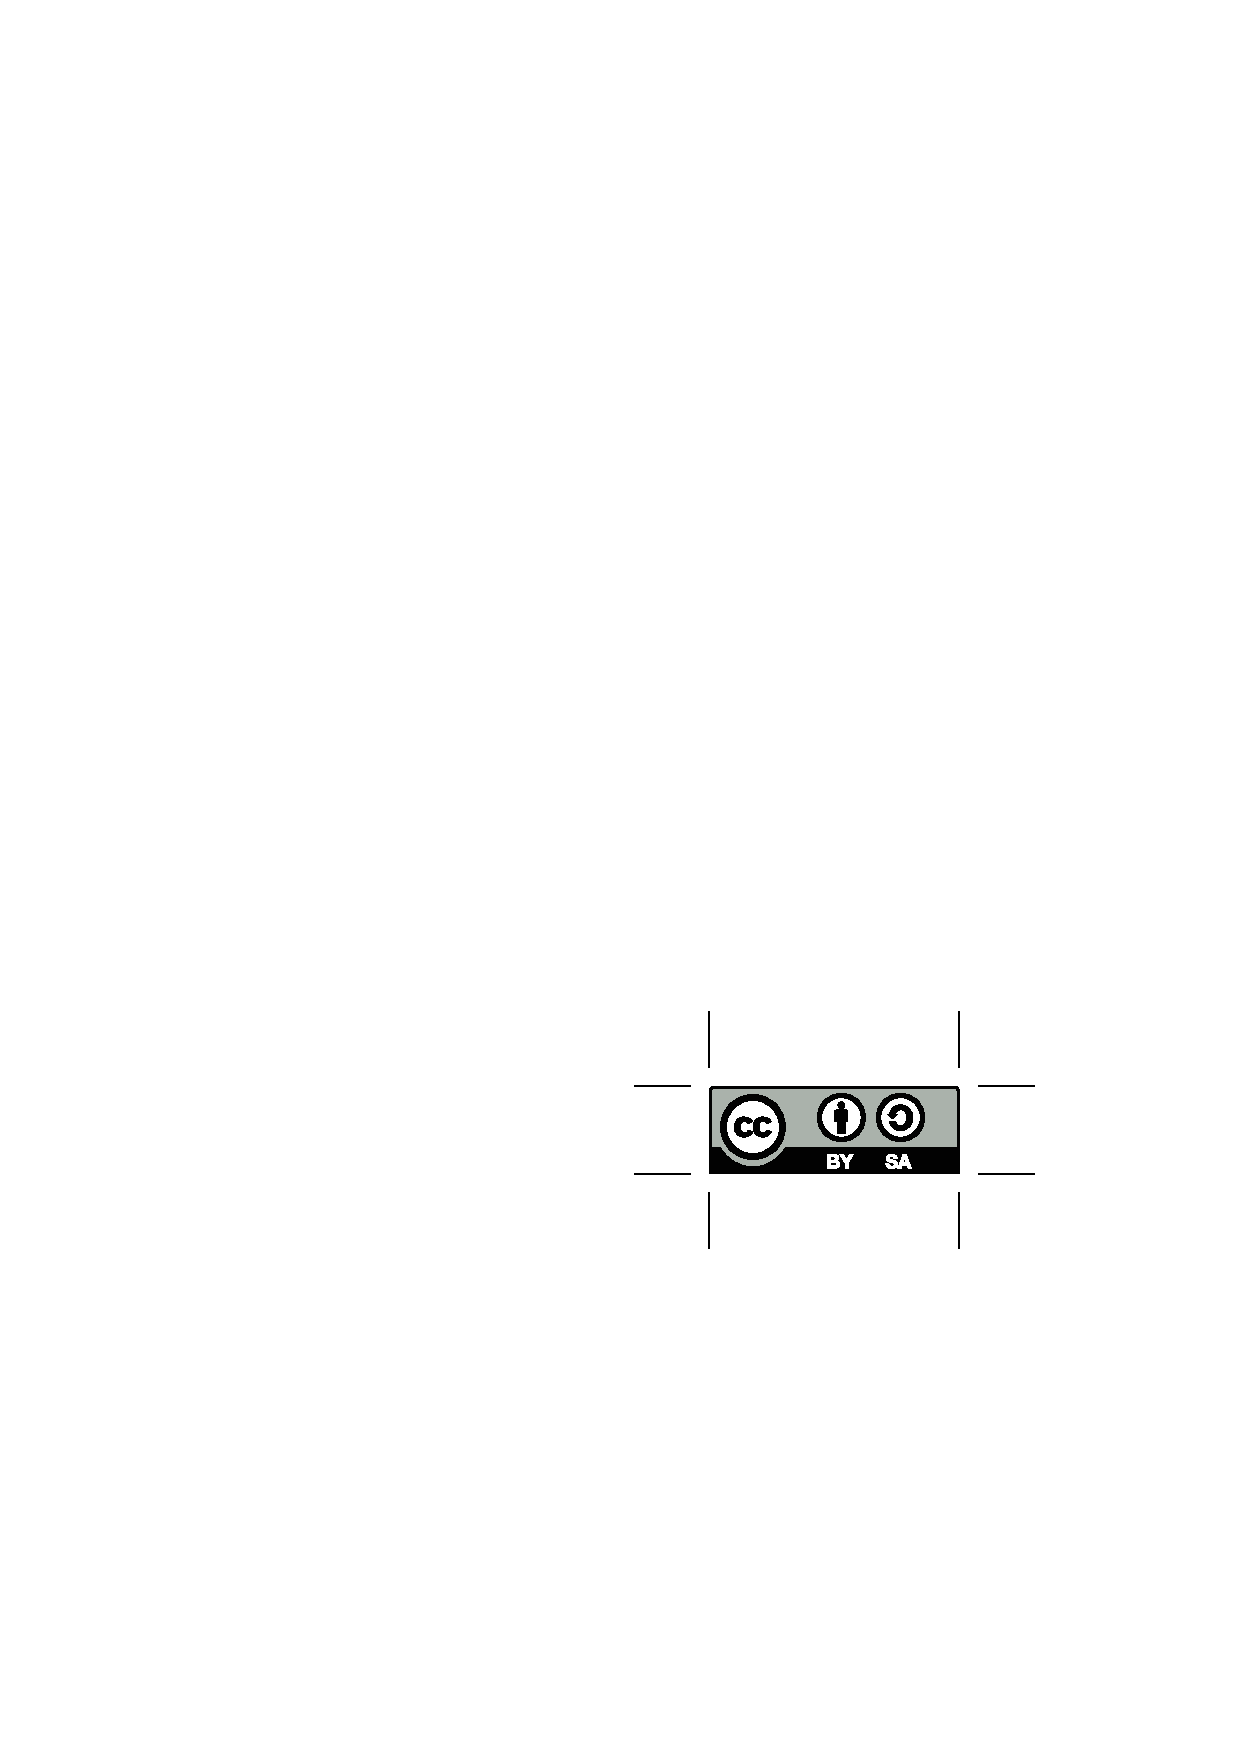
\includegraphics[scale=0.5]{pics/by-sa}
\vspace*{1mm}
\\
\hbox{\parbox{.7\textwidth}
{This work is licensed under the Creative Commons Attribution-ShareAlike
4.0 International License.
To view a copy of this license, visit\\
\texttt{http://creativecommons.org/licenses/by-sa/4.0/}}}

%\ 

%\noindent{\tt
%http://www.createspace.com/4122116
%\\
%\\
%ISBN-13: 978-1481918473
%\\
%ISBN-10: 1481918478
%}


\thispagestyle{empty}
\newpage
{\sloppy
\tableofcontents
}

\chapter*{Introduction}
\addcontentsline{toc}{chapter}{Introduction}
\addtocontents{toc}{\protect\begin{quote}}

This book is meant to be 
rigorous, 
conservative, 
elementary and
minimalist.
At the same time it includes about the maximum what students can absorb in one semester.

Approximately one-third of the material used to be covered in high school, but not any more.

The present book is based 
on the courses given by the author 
at the Pennsylvania State University
as an introduction to the foundations of geometry.
The lectures were oriented to sophomore and senior university students.  
These students already had a calculus course.
In particular, they are familiar with the real numbers and continuity.
It makes it possible to cover the material faster 
and  in a more rigorous way
than it could be done in high school.

\section*{Prerequisite}
\addtocontents{toc}{Prerequisite.}

The students should be familiar 
with the following topics.
\begin{itemize}
\item Elementary set theory: 
$\in$,
$\cup$, 
$\cap$,
$\backslash$,
$\subset$,~$\times$.
\item Real numbers: intervals, inequalities, algebraic identities.
\item Limits, continuous functions and the intermediate value theorem.
\item Standard functions: 
absolute value, 
natural logarithm,
exponential function. 
Occasionally, trigonometric functions  are used, 
but these parts can be ignored.
\item  Chapter~\ref{chap:trans} uses matrix algebra of $2{\times}2$-matrices.
\item To read Chapter~\ref{chap:sphere}, it is better to have some previous experience with the {}\emph{scalar product}, also known as {}\emph{dot product}.
\item To read Chapter~\ref{chap:complex}, it is better to have some previous experience with complex numbers.
\end{itemize} 

\section*{Overview}
\addtocontents{toc}{Overview.}

We use the so called {}\emph{metric approach} introduced by Birkhoff.
It means that we define the Euclidean plane as a {}\emph{metric space} which satisfies a list of properties ({}\emph{axioms}).
This way we minimize the tedious parts
which are unavoidable in the more classical Hilbert's approach.
At the same time the students have a chance to learn basic geometry of metric spaces.

Here is a dependency graph of the chapters.

\begin{figure}[h!]
\centering
\begin{tikzpicture}[->,>=stealth',shorten >=1pt,auto,scale=1.4,
  thick,main node/.style={circle,draw,font=\sffamily\bfseries,minimum size=8mm}]

  \node[main node] (1) at (1,15/6) {\ref{chap:metr}};
  \node[main node] (2) at (2,15/6){\ref{chap:axioms}};
  \node[main node] (3) at (3,15/6) {\ref{chap:half-planes}};
  \node[main node] (4) at (4,15/6) {\ref{chap:cong}};
  \node[main node] (5) at (3.5,10/6) {\ref{chap:perp}};
  \node[main node] (6) at (4.5,10/6) {\ref{chap:parallel}};
  \node[main node] (61) at (4,5/6) {\ref{chap:angle-sum}};
  \node[main node] (7) at (5,5/6) {\ref{chap:triangle}};
  \node[main node] (8) at (3,5/6){\ref{chap:inscribed-angle}};
  \node[main node] (9) at (2,5/6) {\ref{chap:inversion}};
  \node[main node] (10) at (2.5,10/6) {\ref{chap:non-euclid}};
  \node[main node] (11) at (1.5,10/6){\ref{chap:poincare}};
  \node[main node] (12) at (.5,10/6) {\ref{chap:h-plane}};
  \node[main node] (13) at (1.5,0) {\ref{chap:trans}};
  \node[main node] (14) at (0.5,0) {\ref{chap:proj}};
  \node[main node] (15) at (1,5/6) {\ref{chap:sphere}};
  \node[main node] (16) at (0,5/6) {\ref{chap:klein}};
  \node[main node] (17) at (2.5,0) {\ref{chap:complex}};
  \node[main node] (18) at (3.5,0) {\ref{chap:car}};
  \node[main node] (19) at (4.5,0) {\ref{chap:area}};

  \path[every node/.style={font=\sffamily\small}]
   (1) edge node[right]{}(2)
   (2) edge node[right]{}(3)
   (3) edge node[right]{}(4)
   (4) edge node[right]{}(5)
   (5) edge node[right]{}(6)
   (6) edge node[right]{}(61)
   (61) edge node[right]{}(8)
   (61) edge node[right]{}(7)
   (61) edge node[right]{}(19)
   (9) edge node[right]{}(13)
   (13) edge node[right]{}(14)
   (61) edge node[right]{}(18)
   (8) edge node[right]{}(9)
   (9) edge node[right]{}(11)
   (9) edge node[right]{}(15)
   (9) edge node[right]{}(17)
   (5) edge node[right]{}(10)
   (10) edge node[right]{}(11)
   (11) edge node[right]{}(12)
   (14) edge node[right]{}(16)
   (15) edge node[right]{}(16)
   (12) edge node[dashed,right]{}(16);
\end{tikzpicture}
\end{figure}


In (\ref{chap:metr}) we give all the definitions necessary to formulate the axioms;
it includes metric space, 
lines, 
angle measure, 
continuous maps and congruent triangles.


Further we do Euclidean geometry:
(\ref{chap:axioms}) Axioms and immediate corollaries;
(\ref{chap:half-planes}) Half-planes and continuity;
(\ref{chap:cong}) Congruent triangles;
(\ref{chap:perp}) Circles, motions, perpendicular lines;
(\ref{chap:parallel}) Similar triangles and (\ref{chap:angle-sum}) Parallel lines  
--- these are the first two chapters where we use Axiom \ref{def:birkhoff-axioms:4}, an equivalent of Euclid's parallel postulate.
In (\ref{chap:triangle}) we give the most classical theorem of triangle geometry;
this chapter is included mainly as an illustration.


In the following two chapters we discuss geometry of circles on the Euclidean plane:
(\ref{chap:inscribed-angle}) Inscribed angles; (\ref{chap:inversion}) Inversion.
It  will be used to construct the model of the hyperbolic plane.

Further 
we discuss non-Euclidean geometry:
(\ref{chap:non-euclid})
Neutral geometry --- geometry without the parallel postulate;
(\ref{chap:poincare})
Conformal disc model ---
this is a construction of the hyperbolic plane,
an example of a neutral plane which is not Euclidean.
In (\ref{chap:h-plane}) we discuss geometry of the constructed hyperbolic plane --- this is the highest point in the book.

In the reamining chapters we discuss some additional topics:
(\ref{chap:trans}) Affine geometry;
(\ref{chap:proj}) Projective geometry;
(\ref{chap:sphere}) Spherical geometry;
(\ref{chap:klein}) Projective model of the hyperbolic plane;
(\ref{chap:complex}) Complex coordinates;
(\ref{chap:car}) Geometric constructions;
(\ref{chap:area}) Area.
The proofs in these chapters are not completely rigorous.

We encourage to use the visual assignments available at the author's website.

\section*{Disclaimer}

It is  impossible to find the original reference to most of the theorems discussed here, so I do not even try to.
Most of the proofs discussed in the book 
already appeared in the Euclid's Elements.

\section*{Recommended books}

\begin{itemize}
\item Kiselev's textbook \cite{kiselev} ---
a classical book for school students.
Should help if you have trouble following this book.

\item Moise's book, \cite{moise} ---
should be good for further study.

\item Greenberg's book \cite{greenberg}  --- a historical tour in the axiomatic systems of various geometries.

\item Prasolov's book \cite{prasolov} is perfect to master your problem-solving skills.

\item Akopyan's book \cite{akopyan} --- a collection of problems formulated in figures.

\item Methodologically my lectures
were very close to Sharygin's  textbook \cite{sharygin}.
This is the greatest textbook in geometry for school students,
I recommend it to anyone who can read Russian.


\end{itemize}

\section*{Acknowlegments}

Let me thank  
Matthew Chao, 
Svetlana Katok, 
Alexander Lytchak,
Alexei Novi\-kov
and Lukeria Petrunina
for useful suggestions and correcting the misprints.






\addtocontents{toc}{\protect\end{quote}}


\chapter{Preliminaries}\label{chap:metr}
\addtocontents{toc}{\protect\begin{quote}}

\section*{What is the axiomatic approach?}
\addtocontents{toc}{What is the axiomatic approach?}

In the axiomatic approach,
one defines the plane as anything which satisfies 
a given list of properties.
These properties are called {}\emph{axioms}.
Axiomatic system for the theory 
is like the rules for a game.
Once the axiom system is fixed, a statement is considered to be true if it follows from the axioms and nothing else is considered to be true.

The formulations of the first axioms were not rigorous at all.
For example, Euclid described a {}\emph{line} as {}\emph{breadthless length}
and {}\emph{straight line} as a line which {}\emph{lies evenly with the points on itself}.
On the other hand,
these formulations were sufficiently clear, 
so that one mathematician could understand the other.

The best way to understand an axiomatic system
is to make one by yourself.
Look around and choose a physical model 
of the Euclidean plane;
imagine an infinite and perfect surface of a chalk board. 
Now try to collect the key observations
about this model.
Assume for now that we have intuitive understanding of such notions as {}\emph{line} and {}\emph{point}.
\begin{enumerate}[(i)]
 \item\label{preaxiomI} We can measure distances between points.
 \item\label{preaxiomII} We can draw a unique line 
 which passes thru two given points.
 \item\label{preaxiomIII} We can measure angles.
 \item\label{preaxiomIV} If we rotate or shift we will not see the difference.
 \item\label{preaxiomV} If we change scale we will not see the difference.
\end{enumerate}
These observations are good to start with.
Further we will develop the language
to reformulate them rigorously.

\section*{What is a model?}
\addtocontents{toc}{What is a model?}

The Euclidean plane can be defined rigorously the following way:

{}\emph{Define a {}\emph{point} in the Euclidean plane as a pair of real numbers $(x,y)$ and define the {}\emph{distance} between the two points $(x_1,y_1)$ and $(x_2,y_2)$ by the following formula:}
\[\sqrt{(x_1-x_2)^2+(y_1-y_2)^2}.\]

That is it!
We gave a {}\emph{numerical model} of Euclidean plane;
it builds the Euclidean plane from the real numbers
while the latter is assumed to be known.

Shortness is the main advantage of the model approach,
but it is not intuitively clear why we define points and the distances this way.

On the other hand, the observations made in the previous section are  intuitively obvious ---
this is the main advantage of the axiomatic approach.

An other advantage lies in the fact that the axiomatic approach is easily adjustable. 
For example, we may remove one axiom from the list,
or exchange it to another axiom. 
We will do such modifications in Chapter \ref{chap:non-euclid} and further.

\section*{Metric spaces}
\addtocontents{toc}{Metric spaces.}

The notion of metric space provides 
a rigorous way to say: {}\emph{``we can measure distances between points''}.
That is, instead of (\ref{preaxiomI}) on page \pageref{preaxiomI},
we can say {}\emph{``Euclidean plane is a metric space''}.

\begin{thm}{Definition}\label{def:metric-space}
Let $\mathcal X$ be a nonempty set and 
$d$ be a function
which returns a real number $d(A,B)$
for any pair $A,B\in\mathcal X$.
Then $d$
is called \index{metric}\emph{metric} on 
$\mathcal X$ if for any
$A,B,C\in \mathcal X$, the following conditions are satisfied.
\begin{enumerate}[(a)]
\item\label{def:metric-space:a} Positiveness: 
$$d(A,B)\ge 0.$$
\item\label{def:metric-space:b}  $A=B$ if and only if 
$$d(A,B)=0.$$
\item\label{def:metric-space:c} Symmetry: $$d(A, B) = d(B, A).$$
\item\label{def:metric-space:d} Triangle inequality: 
$$d(A, C) \le d(A, B) + d(B, C).$$
\end{enumerate}
A \index{metric space}\emph{metric space} is a set with a metric on it. 
More formally, a metric space is a pair $(\mathcal X, d)$ where $\mathcal X$ is a set and $d$ is a metric on~$\mathcal X$.

The elements of $\mathcal X$ are called \index{point}\emph{points} of the metric space.
Given two points $A,B\z\in \mathcal X$, 
the value $d(A, B)$ is called \index{distance}\emph{distance} from $A$ to~$B$.
\end{thm}

\section*{Examples}
\addtocontents{toc}{Examples.}

\begin{itemize}
\item {}\emph{Discrete metric.} Let $\mathcal X$ be an arbitrary set. 
For any $A,B\z\in\mathcal X$, 
set $d(A,B)\z=0$ if $A=B$ and $d(A,B)=1$ otherwise.
The metric $d$ is called \index{discrete metric}\emph{discrete metric} on~$\mathcal X$.
\item\index{real line}\emph{Real line.} Set of all real numbers ($\mathbb{R}$) with metric defined as 
$$d(A,B)\df|A-B|.$$
\item {}\emph{Metrics on the plane.}
Let us denote by $\mathbb{R}^2$ the set of all pairs $(x,y)$ of real numbers.
Assume $A=(x_A,y_A)$ and $B=(x_B,y_B)$ are arbitrary points in~$\mathbb{R}^2$.
One can equip $\mathbb{R}^2$ with the following metrics:
\begin{itemize}
\item\index{Euclidean metric}\emph{Euclidean metric,} denoted by \index{d@$d_1$, $d_2$, $d_\infty$}$d_2$ and defined as \label{def:d_2}
$$d_2(A,B)=\sqrt{(x_A-x_B)^2+(y_A-y_B)^2}.$$
\item\label{Manhattan plane}\index{Manhattan plane}\emph{Manhattan metric,} denoted by $d_1$ and defined as 
$$d_1(A,B)=|x_A-x_B|+|y_A-y_B|.$$
\item{}\emph{Maximum metric,} denoted by $d_\infty$ and defined as 
$$d_\infty(A,B)=\max\{|x_A-x_B|,|y_A-y_B|\}.$$
\end{itemize}
\end{itemize}

\begin{thm}{Exercise}\label{ex:d_1+d_2+d_infty}
Prove that the following functions are metrics on $\mathbb{R}^2$:
(a)~$d_1$; (b)~$d_2$; (c)~$d_\infty$.
\end{thm}


\section*{Shortcut for distance}
\addtocontents{toc}{Shortcut for distance.}

Most of the time,  
we study only one metric on the space.
Therefore, we will not need to name the metric function each time.

Given a metric space $\mathcal X$,
the distance between points $A$ and $B$ will be further denoted by 
$$AB
\quad
\text{or}
\quad
d_{\mathcal X}(A,B);$$
the latter is used only if we need to emphasize, that $A$ and $B$ are points of the metric space~$\mathcal X$.

For example, the triangle inequality can be written as 
$$AC\le AB+BC.$$

For the multiplication, we will always use ``$\cdot$'',
so $AB$ should not be confused with $A\cdot B$.

\section*{Isometries, motions and lines}
\addtocontents{toc}{Isometries, motions and lines.}

In this section, we define {}\emph{lines} in a metric space.
Once it is done the sentence  {}\emph{``We can draw a unique line which passes thru two given points.''} becomes rigorous; see (\ref{preaxiomII}) on page \pageref{preaxiomII}. 

Recall that a map $f\:\mathcal{X}\to\mathcal{Y}$
is a \index{bijection}\emph{bijection},
if it gives an exact pairing of the elements of two sets.
Equivalently, $f\:\mathcal{X}\to\mathcal{Y}$ is a bijection, if it has an \index{inverse}\emph{inverse};
that is, a map $g\:\mathcal{Y}\to\mathcal{X}$
such that 
$g(f(A))\z=A$   for any $A\in\mathcal{X}$
and
$f(g(B))\z=B$ for any $B\in\mathcal{Y}$. 

\begin{thm}{Definition}\label{def:isom}
Let $\mathcal X$ and $\mathcal Y$ be two metric spaces and $d_{\mathcal X}$, $d_{\mathcal Y}$ be their metrics. 
The map 
$$f\:\mathcal X \z\to \mathcal Y$$ 
is
called \index{distance-preserving map}\emph{distance-preserving} if 
$$d_{\mathcal Y}(f(A), f(B))
 = d_{\mathcal X}(A,B)$$
for any $A,B\in {\mathcal X}$.

A bijective distance-preserving map is called an \index{isometry}\emph{isometry}. 

Two metric spaces are called
\emph{isometric} if there exists an isometry from one to the other.

The isometry from a metric space to itself 
is also called a \index{motion}\emph{motion} of the space.
\end{thm}

\begin{thm}{Exercise}\label{ex:dist-preserv=>injective}
Show that any distance-preserving map  is \index{injective map}\emph{injective};
that is, if $f\:\mathcal X\to\mathcal Y$ is a distance-preserving map, 
then $f(A)\ne f(B)$ for any pair of distinct points $A,  B\in \mathcal X$.
\end{thm}

\begin{thm}{Exercise}\label{ex:motion-of-R}
Show that if $f\:\mathbb{R}\to\mathbb{R}$ is a motion of the real line,
then either (a)
$f(x)=f(0)+x$ for any $x\in \mathbb{R}$,  
or (b)
$f(x)=f(0)-x$ for any $x\in \mathbb{R}$. 

\end{thm}

\begin{thm}{Exercise}\label{ex:d_1=d_infty}
Prove that $(\mathbb{R}^2,d_1)$ is isometric to $(\mathbb{R}^2,d_\infty)$.
\end{thm}

\begin{thm}{Advanced exercise}\label{ad-ex:motions of Manhattan plane}
Describe all the motions of the Manhattan plane, defied on page~\pageref{Manhattan plane}.
\end{thm}

If $\mathcal X$ is a metric space and $\mathcal Y$ is a subset of $\mathcal X$,
then a metric on $\mathcal Y$ can be obtained by restricting the metric from~$\mathcal X$. 
In other words, 
the distance between two points of $\mathcal Y$ is defined to be the distance between these points in =~$\mathcal X$.
This way any subset of a metric space can be also considered as a metric space. 

\begin{thm}{Definition}\label{def:line}
A subset $\ell$ of metric space is called a \index{line}\emph{line}, if it is isometric to the real line.
\end{thm}

Note that a space with a discrete metric has no lines.
The following picture shows examples of lines on the Manhattan plane $(\mathbb{R}^2,d_1)$. 

\begin{center}
\begin{lpic}[t(0mm),b(0mm),r(0mm),l(0mm)]{pics/mink-lines(1)}
\end{lpic}
\end{center}

\begin{thm}{Exercise}\label{ex:y=|x|}
Consider the graph $y=|x|$ in =~$\mathbb{R}^2$.
In which of the following spaces 
(a) $(\mathbb{R}^2,d_1)$, 
(b) $(\mathbb{R}^2,d_2)$, 
(c) $(\mathbb{R}^2,d_\infty)$ 
does it form a line? 
Why?
\end{thm}

\begin{thm}{Exercise}\label{ex:2mid}
How many points $M$ are there on the line $(A B)$ for which we have
\begin{enumerate}
\item $AM= MB$ ?
\item $AM= 2\cdot MB$ ?
\end{enumerate}
\end{thm}

\section*{Half-lines and segments}
\addtocontents{toc}{Half-lines and segments.}

Assume there is a line $\ell$ passing thru
two distinct points $P$ and =~$Q$.
In this case we might denote $\ell$ as $(PQ)$.
There might be more than one line thru $P$ and $Q$,
but if we write \index{60@$(PQ)$, $[PQ)$, $[PQ]$}$(PQ)$ we assume that we made a choice of such line. 

Let us denote by $[P Q)$ the \index{half-line}\emph{half-line}
which starts at $P$ and contains~$Q$. 
Formally speaking, $[P Q)$ is a subset of $(P Q)$ which corresponds to $[0,\infty)$ under an isometry $f\:(P Q)\to \mathbb{R}$ such that $f(P)=0$ and $f(Q)>0$.

\begin{thm}{Exercise}\label{ex:trig==}
Show that if $X\in [PQ)$, then 
$QX=|PX-PQ|$.
\end{thm}

The subset of line $(P Q)$ between $P$ and $Q$ is called the \index{segment}\emph{segment} between $P$ and $Q$ and denoted by~$[P Q]$.
Formally, the segment can be defined as the intersection of two half-lines: $[P Q]=[P Q)\cap[Q P)$.


\section*{Angles}
\addtocontents{toc}{Angles.}

Our next goal is to introduce {}\emph{angles} and {}\emph{angle measures}; 
after that, the statement {}\emph{``we can measure angles''} will become rigorous;
see (\ref{preaxiomIII}) on page \pageref{preaxiomIII}.

\begin{wrapfigure}{r}{40mm}
\begin{lpic}[t(-4mm),b(-2mm),r(0mm),l(3mm)]{pics/angle(1)}
\lbl[rb]{2,5;$O$}
\lbl[rb]{16,25;$B$}
\lbl[b]{31,5;$A$}
\lbl[lb]{12,7;$\alpha$}
\end{lpic}
\end{wrapfigure}

An ordered pair of half-lines which start at the same point is called an \index{angle}\emph{angle}.
The angle $AOB$ (also denoted by \index{10@$\angle$}$\angle AOB$) is formed by two half-lines $[OA)$ and $[OB)$.
In this case the point $O$ is called the \index{vertex of the angle}\emph{vertex} of the angle.

Intuitively, the angle measure tells how much one has to rotate the first half-line counterclockwise, so it gets the position of the second half-line of the angle. 
The full turn is assumed to be $2\cdot\pi$;
it corresponds to the angle measure in radians.

The angle measure of $\angle AOB$ is denoted by \index{12@$\measuredangle$}$\measuredangle AOB$;
it is a real number in the interval $(-\pi,\pi]$. 

The notations $\angle AOB$ and $\measuredangle AOB$ look similar,
they also have close but different meanings, 
which better not be confused.
For example, the equality 
$\angle AOB=\angle A'O'B'$
means that
$[OA)=[O'A')$ and $[OB)\z=[O'B')$;
in particular, $O=O'$.
On the other hand the equality 
$\measuredangle AOB\z=\measuredangle A'O'B'$ 
means only equality of two real numbers;
in this case $O$ may be distinct from~$O'$.

Here is the first property of angle measure which will become a part of the axiom.

\textit{Given a half-line $[O A)$ and $\alpha\in(-\pi,\pi]$ there is a unique half-line $[O B)$ such that $\measuredangle A O B= \alpha$.}





\section*{Reals modulo $\bm{2\cdot\pi}$}
\addtocontents{toc}{Reals modulo $2\cdot\pi$.}

Consider three half-lines starting from the same point,
 $[O A)$, $[O B)$ and~$[O C)$.
They make three angles $A O B$, $B O C$ and $A O C$,
so the value $\measuredangle A O C$ should coincide with
the sum $\measuredangle A O B+\measuredangle B O C$ up to full rotation.
This property will be expressed by the formula 
$$\measuredangle A O B+\measuredangle B O C\equiv \measuredangle A O C,$$
where \index{34@$\equiv$}``$\equiv$'' is a new notation which we are about to introduce.
The last identity will become a part of the axiom.

%???how to say who is pi???

We will write 
\begin{align*}
\alpha&\equiv\beta
\intertext{or}
\alpha&\equiv\beta\pmod{2\cdot\pi}
\end{align*}
if $\alpha=\beta+2\cdot\pi\cdot n$
for some integer~$n$.
In this case we say 
$$\textit{``$\alpha$ is equal to $\beta$ modulo $2\cdot\pi$''}.$$
For example 
$$-\pi
\equiv
\pi\equiv 3\cdot\pi
\quad
\text{and}
\quad
\tfrac12\cdot\pi
\equiv
-\tfrac32\cdot\pi.$$

The introduced relation ``$\equiv$'' behaves as an equality sing,
but
\[\dots\equiv\alpha-2\cdot\pi\equiv \alpha\equiv \alpha+2\cdot\pi\equiv \alpha+4\cdot\pi\equiv\dots;\] 
that is, if the angle measures differ by full turn,
then they are considered to be the same.

With ``$\equiv$'', we can do addition, subtraction and multiplication with integer numbers without getting into trouble.
That is, if
$$\alpha\equiv\beta
\quad
\text{and}
\quad
\alpha'\equiv \beta',$$ 
then
$$\alpha+\alpha'\equiv\beta+\beta',
\quad
\alpha-\alpha'\equiv \beta-\beta'
\quad 
\text{and}
\quad
n\cdot\alpha\equiv n\cdot\beta$$
for any integer~$n$.
But ``$\equiv$'' does not in general respect multiplication with non-integer numbers; for example 
$$\pi
\equiv 
-\pi
\quad
\text{but}
\quad
\tfrac12\cdot\pi
\not\equiv
-\tfrac12\cdot\pi.$$ 

\begin{thm}{Exercise}\label{ex:2a=0}
Show that $2\cdot\alpha\equiv0$ if and only if $\alpha\equiv0$ or $\alpha\equiv\pi$.
\end{thm}

\section*{Continuity}
\addtocontents{toc}{Continuity.}

The angle measure is also assumed to be continuous.
Namely, the following property of angle measure will become a part of the axiom.

\textit{The function}
$$\measuredangle\:(A,O,B)\mapsto\measuredangle A O B$$
\textit{is continuous at any triple of points $(A,O,B)$
such that $O\ne A$ and $O\ne B$ and $\measuredangle A O B\ne\pi$.}

To explain this property, we need to extend the notion of {}\emph{continuity} to the functions between metric spaces.
The definition is a straightforward generalization of the standard definition for the real-to-real functions.

Further, let $\mathcal X$ and $\mathcal Y$ be two metric spaces,
and $d_{\mathcal X}$, $d_{\mathcal Y}$ be their metrics.

A map $f\:\mathcal X\to\mathcal Y$ is called continuous at point $A\in \mathcal X$
if for any  $\epsilon>0$ there is $\delta>0$, such that 
\[d_{\mathcal X}(A,A')
<
\delta
\quad
\Rightarrow
\quad
d_{\mathcal Y}(f(A),f(A'))
<
\epsilon.\]

One may define a continuous map of several variables the same way.
Assume $f(A,B,C)$ is a function which returns a point in the space $\mathcal Y$ for a triple of points $(A,B,C)$
in the space~$\mathcal X$.
The map $f$ might be defined only for some triples in~$\mathcal X$.

Assume $f(A,B,C)$ is defined.
Then, we say that $f$ is continuous at the triple $(A,B,C)$ 
if for any $\epsilon>0$ there is $\delta>0$ such that 
\[d_{\mathcal Y}(f(A,B,C),f(A',B',C'))<\epsilon.\]
if $d_{\mathcal X}(A,A')<\delta$, $d_{\mathcal X}(B,B')<\delta$ and $d_{\mathcal X}(C,C')<\delta$.


\begin{thm}{Exercise}\label{ex:dist-cont}
Let $\mathcal{X}$ be a metric space.
\begin{enumerate}[(a)]
\item\label{ex:dist-cont:a} Let $A\in \mathcal{X}$ be a fixed point.
Show that the function 
$$f(B)\df
d_{\mathcal{X}}(A,B)$$ 
is continuous at any point~$B$.
\item Show that $d_{\mathcal{X}}(A,B)$ is continuous  at any pair $A,B\in \mathcal{X}$.
\end{enumerate}

\end{thm}

\begin{thm}{Exercise}\label{ex:comp+cont}
Let $\mathcal{X}$, $\mathcal{Y}$ and $\mathcal{Z}$ be a metric spaces.
Assume that the functions $f\:\mathcal{X}\to\mathcal{Y}$
and $g\:\mathcal{Y}\to\mathcal{Z}$ are continuous at any point,
and $h=g\circ f$ is its composition;
that is, $h(A)=g(f(A))$ for any $A\in \mathcal{X}$.
Show that $h\:\mathcal{X}\to\mathcal{Z}$ is continuous at any point.
\end{thm}

\begin{thm}{Exercise}\label{ex:isom-cont}
Show that any distance-preserving map is continuous.
\end{thm}




\section*{Congruent triangles} 
\addtocontents{toc}{Congruent triangles.}

Our next goal is to give a rigorous meaning for  (\ref{preaxiomIV}) on page \pageref{preaxiomIV}.
To do this, we introduce the notion of {}\emph{congruent triangles}
so instead of {}\emph{``if we rotate or shift we will not see the difference''} we say that for triangles, the side-angle-side congruence holds;
that is, two triangles are congruent if they have two pairs of equal sides and the same angle measure between these sides.

An {}\emph{ordered} triple of distinct points in a metric space $\mathcal{X}$, 
say $A,B,C$,
is called a \index{triangle}\emph{triangle $ABC$}\label{page:def:triangle} (briefly  \index{20@$\triangle$}$\triangle A B C$).
Note that the triangles $A B C$ and $ A C B$ are considered as different.

Two triangles $ A' B' C'$ and $ A B C$ are called 
\index{triangle!congruent triangles}
\index{congruent triangles}\emph{congruent}
(written as \index{32@$\cong$}$\triangle A' B' C'\z\cong\triangle A B C$) if there is a motion $f\:\mathcal{X}\to\mathcal{X}$ such that 
\[A'\z=f(A),
\quad
B'=f(B)
\quad
\text{and}
\quad
C'=f(C).\]

Let $\mathcal X$ be a metric space,
and $f,g\:\mathcal X\to\mathcal X$ be two motions.
Note that the inverse $f^{-1}:\mathcal X\to\mathcal X$,
as well as the composition $f\circ g:\mathcal X\to\mathcal X$
are also motions.

It follows that ``$\cong$'' is an \index{equivalence relation}\emph{equivalence relation};
that is, any triangle congruent to itself, 
and the following two conditions hold.
\begin{itemize} 
\item If $\triangle A' B' C'\z\cong\triangle A B C$, then $\triangle A B C\z\cong\triangle A' B' C'$.
\item If $\triangle A'' B'' C''\z\cong\triangle A' B' C'$ and $\triangle A' B' C'\z\cong\triangle A B C$,
then 
$$\triangle A'' B'' C''\cong\triangle A B C.$$
\end{itemize}


Note that if $\triangle A' B' C'\z\cong\triangle A B C$,
then $AB\z=A'B'$,
$BC=B'C'$ and $CA=C'A'$.

For a discrete metric, as well as some other metrics, 
the converse also holds.
The following example shows that it does not hold in the Manhattan plane.

\parbf{Example.}\label{example:isometric but not congruent} Consider three points 
$A=(0,1)$, $B=(1,0)$ and $C\z=(-1,0)$ on the Manhattan plane $(\mathbb{R}^2,d_1)$.
Note that
$$d_1(A,B)=d_1(A,C)=d_1(B,C)=2.$$

\begin{wrapfigure}[7]{o}{46mm}
\begin{lpic}[t(-3mm),b(0mm),r(0mm),l(2mm)]{pics/mink-ABC(1)}
\lbl[b]{21,23;$A$}
\lbl[lt]{37,4;$B$}
\lbl[rt]{6,4;$C$}
\end{lpic}
\end{wrapfigure}

On one hand,
$$\triangle ABC\cong \triangle ACB.$$

Indeed, 
it is easy to see that
 the map $(x,y)\mapsto (-x,y)$ is a motion of $(\mathbb{R}^2,d_1)$,
which sends $A\mapsto A$, $B\mapsto C$ and $C\mapsto B$.

On the other hand,
$$\triangle ABC\z\ncong \triangle BCA.$$

%???(
Indeed, arguing by contradiction, assume that $f$ is a motion of $(\mathbb{R}^2,d_1)$ which sends $A\mapsto B$ and $B\mapsto C$.
%???)
Note that a point $M$ is a midpoint\footnote{$M$ is a midpoint of $A$ and $B$ if $d_1(A,M)=d_1(B,M)=\tfrac12\cdot d_1(A,B)$.} of $A$ and $B$ if and only if $f(M)$ is a midpoint of $B$ and~$C$.

The set of midpoints for $A$ and $B$ is infinite, it contains all points $(t,t)$ for $t\in[0,1]$ (it is the dark gray segment on the picture above).
On the other hand, the midpoint for $B$ and $C$ is unique (it is the black point on the picture).
Thus, the map $f$ cannot be bijective, a contradiction.

\addtocontents{toc}{\protect\end{quote}}
%\part*{Euclidean geometry}
\addtocontents{toc}{\protect\begin{center}}
\addtocontents{toc}{\large{\bf Euclidean geometry}}
\addtocontents{toc}{\protect\end{center}}
\chapter{Axioms}
\label{chap:axioms}
\addtocontents{toc}{\protect\begin{quote}}

%(???

\vfill

A system of axioms appears already in Euclid's ``Elements'' --- the most successful and influential textbook ever written.

The systematic study of geometries as axiomatic systems
 was
triggered by the discovery of non-Euclidean geometry.
The branch of mathematics, emerging this way, is called ``Foundations of geometry''.

The most popular system of axiom
was proposed in 1899 by David Hilbert.
This is also the first rigorous system by modern standards.
It contains twenty axioms in five groups, six ``primitive notions'', and three ``primitive terms'';
these are not defined in terms of previously defined concepts.

Later a number of different systems were proposed.
It is worth mentioning
the system of Alexandr Alexandrov \cite{alexandrov} which is very intuitive and elementary, 
the system of Friedrich Bachmann \cite{bachmann} which is based on the concept of symmetry,
and the system of Alfred Tarski \cite{tarski}, which was designed for analysis using mathematical logic.

We will use another system,
which is very close to the one proposed by George Birkhoff in \cite{birkhoff}.
This system is based on the {}\emph{key observations}  (\ref{preaxiomI})--(\ref{preaxiomV}) listed on page~\pageref{preaxiomI}.
The axioms use the notions of 
metric space, 
lines, 
angles,
triangles,
equalities modulo $2\cdot\pi$ ($\equiv$), 
the continuity of maps between metric spaces,
and the congruence of triangles ($\cong$).
All this discussed in the preliminaries.

Our system is build upon metric spaces.
In particular, we use the real numbers as a building block. 
By that reason our approach is not purely axiomatic --- we build the theory upon something else;
it resembles a model-based introduction to Euclidean geometry discussed on page~\pageref{page:model}.
We used this approach to minimize the tedious parts which are unavoidable in purely axiomatic foundations.

%???)

\newpage

\section*{The axioms}
\addtocontents{toc}{The axioms.}

\begin{framed}
\begin{enumerate}[I.]
\item\label{def:birkhoff-axioms:0} The \index{plane!Euclidean plane}\index{Euclidean plane}\emph{Euclidean plane} is a metric space with at least two points.


\item\label{def:birkhoff-axioms:1} 
There is one and only one line, that contains any two given distinct points $P$ and $Q$ in the Euclidean plane.

\item\label{def:birkhoff-axioms:2} 
Any angle $AOB$ in the Euclidean plane 
defines a real number in the interval $(-\pi,\pi]$.
This number is called \index{angle measure}\emph{angle measure of $\angle AOB$}
and denoted by $\measuredangle A O B$.
It satisfies the following conditions:
\begin{enumerate}[(a)]
\item\label{def:birkhoff-axioms:2a} 
Given a half-line $[O A)$ and $\alpha\in(-\pi,\pi]$, 
there is a unique  half-line $[O B)$, 
such that $\measuredangle A O B= \alpha$.
\item\label{def:birkhoff-axioms:2b} 
For any points $A$, $B$, and $C$, distinct from $O$ we have
$$\measuredangle A O B+\measuredangle B O C
\equiv\measuredangle A O C.$$
\item\label{def:birkhoff-axioms:2c} 
The function 
$$\measuredangle\:(A,O,B)\mapsto\measuredangle A O B$$
is continuous at any triple of points $(A,O,B)$,
such that $O\ne A$ and $O\ne B$ and $\measuredangle A O B\ne\pi$.

\end{enumerate}

\item\label{def:birkhoff-axioms:3}  
In the Euclidean plane, we have
$\triangle A B C\cong\triangle A' B' C'$
if and only if 
\begin{align*}
A' B'&=A B, & A' C'&= A C, &&\text{and}
&\measuredangle C' A' B'&=\pm\measuredangle C A B.
\end{align*}
\item\label{def:birkhoff-axioms:4}
If for two triangles $ABC$, $AB'C'$ in the Euclidean plane
and for $k>0$ we have
\begin{align*}
B'&\in [AB),
& C'&\in [AC),
\\
AB'&=k\cdot AB,&
AC'&=k\cdot AC,
\end{align*}
then
\begin{align*}
B'C'&=k\cdot BC,&
\measuredangle ABC&=\measuredangle AB'C',
&
\measuredangle ACB&=\measuredangle AC'B'.
\end{align*}
\end{enumerate}
\end{framed}

From now on,  
we can use no information about the Euclidean plane which does not follow from the five axioms above.

\begin{thm}{Exercise}\label{ex:infinite}
Show that there are (a) an infinite set of points,
(b) an infinite set of lines on the plane.
\end{thm}

\section*{Lines and half-lines}
\addtocontents{toc}{Lines and half-lines.}

\begin{thm}[\abs]{Proposition}\label{lem:line-line}
\let\thefootnote\relax\footnotetext{${}^\a$ A statement marked with ``$\a$'' if Axiom~\ref{def:birkhoff-axioms:4} was not used in its proof.
Ignore this mark for a while; it will be important in Chapter~\ref{chap:non-euclid}, see page \pageref{a-mark}.}
Any two distinct lines intersect at most at one point.
\end{thm}

\parit{Proof.}
Assume that two lines $\ell$ and $m$ intersect at two distinct points $P$ and~$Q$.
Applying Axiom~\ref{def:birkhoff-axioms:1}, we get that $\ell=m$.
\qeds

\begin{thm}{Exercise}\label{ex:[OA)=[OA')}
Suppose $A'\in[OA)$ and $A'\not=O$. 
Show that 
\[[O A)\z=[O A').\]

\end{thm}

\begin{thm}[\abs]{Proposition}\label{prop:point-on-half-line}
Given $r\ge 0$ and a half-line $[O A)$ there is a unique $A'\in [O A)$  such that $O A'=r$.
\end{thm}

\parit{Proof.}
According to definition of half-line, 
there is an isometry 
$$f\:[O A)\to [0,\infty),$$
such that $f(O)=0$.
By the definition of isometry, $O A'=f(A')$ for any $A'\z\in [O A)$.
Thus, $O A'=r$ if and only if $f(A')=r$.

Since isometry has to be bijective, the statement follows.
\qeds

\section*{Zero angle}
\addtocontents{toc}{Zero angle.}

\begin{thm}[\abs]{Proposition}\label{lem:AOA=0}
$\measuredangle A O A= 0$ for any $A\not=O$.
\end{thm}

\parit{Proof.}
According to Axiom~\ref{def:birkhoff-axioms:2b},
$$\measuredangle A O A
+
\measuredangle A O A 
\equiv
\measuredangle A O A.$$
Subtract  $\measuredangle A O A$ from both sides, we get that
$\measuredangle A O A \equiv 0$.

By Axiom~\ref{def:birkhoff-axioms:2}, $-\pi<\measuredangle A O A\le \pi$;
therefore $\measuredangle A O A \z= 0$.
\qeds

\begin{thm}{Exercise}\label{ex:2.4} 
Assume $\measuredangle A O B= 0$.
Show that $[OA)=[OB)$.
\end{thm}

\begin{thm}[\abs]{Proposition}\label{lem:AOB+BOA=0}
For any $A$ and $B$ distinct from $O$,
we have 
$$\measuredangle A O B\equiv-\measuredangle B O A.$$

\end{thm}

\parit{Proof.}
According to Axiom~\ref{def:birkhoff-axioms:2b},
$$\measuredangle A O B+\measuredangle B O A \equiv\measuredangle A O A$$
By Proposition~\ref{lem:AOA=0}, $\measuredangle A O A=0$.
Hence the result.
\qeds

\section*{Straight angle}
\addtocontents{toc}{Straight angle.}

If $\measuredangle A O B=\pi$,
we say that $\angle A O B$ is a 
\index{angle!straight angle}\emph{straight angle}.
Note that by Proposition~\ref{lem:AOB+BOA=0}, 
if $\angle A O B$ is a straight,
then so is $\angle B O A$.

We say that point $O$ \index{between}\emph{lies between} points $A$ and $B$, 
if $O\not= A$, $O\not= B$, and $O\in[A B]$.

\begin{thm}[\abs]{Theorem}\label{thm:straight-angle}
The angle $A O B$ is straight 
if and only if $O$ 
\index{between}\emph{lies between} $A$ and~$B$.
\end{thm}

\begin{wrapfigure}{r}{39mm}
\centering
\includegraphics{mppics/pic-8}
\end{wrapfigure}

\parit{Proof.}
By Proposition~\ref{prop:point-on-half-line},  we may assume that
$O A = O B = 1$.

\parit{``If'' part.}
Assume $O$  
lies between $A$ and~$B$.
Set  $\alpha=\measuredangle A O B$.

Applying Axiom~\ref{def:birkhoff-axioms:2a},
we get a half-line $[OA')$ such that $\alpha\z=\measuredangle B O A'$.
By Proposition~\ref{prop:point-on-half-line}, we can assume that $OA'=1$.
According to Axiom~\ref{def:birkhoff-axioms:3},
\[\triangle AOB\z\cong\triangle BOA'.\]
Let $f$ denotes the corresponding motion of the plane;
that is, $f$ is a motion such that $f(A)=B$, $f(O)=O$, and $f(B)=A'$. 

\begin{wrapfigure}{o}{39mm}
\centering
\includegraphics{mppics/pic-10}
\end{wrapfigure}

Then 
\[(A'B)=f(AB)\ni f(O)=O.\]
Therefore, both lines $(AB)$ and $(A'B)$ contain $B$ and~$O$.
By Axiom~\ref{def:birkhoff-axioms:1}, $(AB)=(A'B)$.

By the definition of the line,
$(AB)$ contains exactly two points $A$ and $B$ on distance $1$ from~$O$.
Since $OA'=1$ and $A'\ne B$, we get that $A=A'$.

By Axiom~\ref{def:birkhoff-axioms:2b} and Proposition~\ref{lem:AOA=0}, we get that
\begin{align*}
2\cdot\alpha&=
\measuredangle AOB+\measuredangle BOA'=
\\
&=\measuredangle AOB+\measuredangle BOA\equiv
\\
&\equiv\measuredangle AOA=
\\
&= 0
\end{align*}
Therefore, by Exercise~\ref{ex:2a=0}, $\alpha$ is either $0$ or~$\pi$.

Since $[OA)\ne [OB)$,  
we have that $\alpha\ne 0$, see Exercise~\ref{ex:2.4}.
Therefore, $\alpha=\pi$.


\parit{``Only if'' part.}
Suppose that $\measuredangle A O B= \pi$.
Consider the line $(OA)$ and choose a point $B'$ on $(OA)$ so that $O$ lies between $A$ and~$B'$.

From above, we have that $\measuredangle AOB'=\pi$.
Applying Axiom~\ref{def:birkhoff-axioms:2a}, 
we get that $[O B)\z=[O B')$.
In particular, $O$ lies between $A$ and~$B$.
\qeds 

A triangle $ABC$ is called 
\index{triangle!degenerate triangle}\index{degenerate! triangle}\emph{degenerate}
if $A$, $B$, and $C$ lie on one line.
The following corollary is just a reformulation of Theorem~\ref{thm:straight-angle}.

\begin{thm}[\abs]{Corollary}\label{cor:degenerate=pi}
A triangle is degenerate if and only if one of its angles is equal to $\pi$ or~$0$.
Moreover in a degenerate triangle the angle measures are $0$, $0$, and $\pi$.
\end{thm}

\begin{thm}{Exercise}\label{ex:lineAOB}
Show that three distinct points $A$, $O$, and $B$ lie on one line if and only if 
$$2\cdot \measuredangle AOB\equiv 0.$$ 

\end{thm}

\begin{thm}{Exercise}\label{ex:ABCO-line}
Let $A$, $B$ and $C$ be three points distinct from~$O$.
Show that $B$, $O$ and $C$ lie on one line if and only if
$$2\cdot \measuredangle AOB\equiv 2\cdot \measuredangle AOC.$$ 

\end{thm}

\begin{thm}{Exercise}\label{ex:infinite-number-of-lines} 
Show that there is a nondegenerate triangle.
\end{thm}

\section*{Vertical angles}
\addtocontents{toc}{Vertical angles.}

A pair of angles $AOB$ and $A'OB'$ 
is called \index{angle!vertical angles}\index{vertical angles}\emph{vertical}
if the point $O$ 
lies between $A$ and $A'$ 
and between $B$ and $B'$ at the same time.


\begin{thm}[\abs]{Proposition}\label{prop:vert}
The vertical angles have equal measures.
\end{thm}


\parit{Proof.}
Assume that the angles $AOB$ and $A'OB'$ are vertical.
Note that $\angle AOA'$ and $\angle BOB'$ are straight.
Therefore, $\measuredangle AOA'\z=\measuredangle BOB'=\pi$.

{

\begin{wrapfigure}[4]{o}{24mm}
\vskip-2mm
\centering
\includegraphics{mppics/pic-12}
\end{wrapfigure}

It follows that
\begin{align*}
0&=\measuredangle AOA'-\measuredangle BOB'\equiv
\\
&\equiv 
\measuredangle AOB+\measuredangle BOA'-\measuredangle BOA'-\measuredangle A'OB'
\equiv
\\
&\equiv\measuredangle AOB-\measuredangle A'OB'.
\end{align*}
Since $-\pi<\measuredangle AOB\le \pi$ and $-\pi<\measuredangle A'OB'\le \pi$, we get that $\measuredangle AOB\z=\measuredangle A'OB'$.
\qeds

}

\begin{thm}{Exercise}\label{ex:O-mid-AB+CD}
Assume $O$ 
is the midpoint for both segments 
$[A B]$ and $[C D]$.
Prove that $A C= B D$. 
\end{thm}




\addtocontents{toc}{\protect\end{quote}}

\chapter{Half-planes}\label{chap:half-planes}
\addtocontents{toc}{\protect\begin{quote}}

This chapter contains long proofs of intuitively evident statements.
It is okay to skip it, but make sure you know definitions of positive/negative angles and that your intuition agrees with \ref{thm:signs-of-triug}, \ref{prop:half-plane}, \ref{cor:half-plane}, \ref{thm:pasch} and \ref{thm:abc}.

 
                            
\section*{Sign of an angle}
\addtocontents{toc}{Sign of an angle.}

The positive and negative angles can be visualized as {}\emph{counterclockwise} and  {}\emph{clockwise} directions; formally, they are defined the following way.

\begin{itemize}
\item The angle $A O B$ is called \index{angle!positive and negative angles}\emph{positive} 
if $0<\measuredangle A O B<\pi$;
\item The  angle $A O B$ is called {}\emph{negative} 
if $\measuredangle A O B<0$.
\end{itemize}

Note that according to the above definitions the straight angle as well as the zero angle 
are neither positive nor negative.

\begin{thm}{Exercise}\label{ex:AOB+<=>BOA-}
Show that $\angle A O B$ is positive if and only if $\angle B O A$ is negative.
\end{thm}

\begin{thm}{Lemma}\label{lem:straight-sign}
Let $\angle AOB$ be straight.
Then $\angle AOX$ is positive 
if and only if $\angle BOX$ is negative.
\end{thm}

\parit{Proof.}
Set $\alpha=\measuredangle AOX$ 
and 
$\beta=\measuredangle BOX$.
Since $\angle AOB$ is straight,
$$\alpha-\beta\equiv \pi.\eqlbl{eq:alpha-beta}$$

It follows that $\alpha=\pi$ $\Leftrightarrow$ $\beta=0$
and $\alpha=0$ $\Leftrightarrow$ $\beta=\pi$.
In these two cases the sing of $\angle AOX$ and $\angle BOX$ are undefined.

In the remaining cases we have $|\alpha|,|\beta|<\pi$.
If $\alpha$ and $\beta$ have the same sign, then $|\alpha-\beta|<\pi$;
the latter contradicts \ref{eq:alpha-beta}.
Hence the statement follows.
\qeds

\begin{thm}{Exercise}\label{ex:PP(PN)}
Assume that the angles $AOB$ and $BOC$ are positive. 
Show that
$$\measuredangle AOB+\measuredangle BOC+\measuredangle COA=2\cdot\pi.$$
if $\angle COA$ is positive,
and
$$\measuredangle AOB+\measuredangle BOC+\measuredangle COA=0.$$
if $\angle COA$ is negative.
\end{thm}




\section*{Intermediate value theorem}
\addtocontents{toc}{Intermediate value theorem.}


\begin{thm}{Intermediate value theorem}\label{thm:intermidiate}
Let $f\:[a,b]\to \mathbb{R}$ be a continuous function.
Assume 
$f(a)$ and $f(b)$ have opposite signs,
then $f(t_0)=0$ for some $t_0\in[a,b]$.
\end{thm}

\begin{wrapfigure}{o}{38mm}
\begin{lpic}[t(-6mm),b(0mm),r(0mm),l(5mm)]{pics/ivt(1)}
\lbl[r]{2,20;$f(b)$}
\lbl[r]{2,1;$f(a)$}
\lbl[tl]{11,8;$t_0$}
\lbl[t]{27.5,8;$b$}
\lbl[b]{7.5,10.5;$a$}
\end{lpic}
\end{wrapfigure}



The intermediate value theorem is assumed to be known;
it should be covered in any calculus course.
We will use the following corollary.

\begin{thm}[\abs]{Corollary}\label{cor:intermidiate}
Assume that for any $t\z\in [0,1]$ we have three points in the plane  $O_t$, $A_t$ and $B_t$, such that 
\begin{enumerate}[(a)]
\item Each  function $t\mapsto O_t$, $t\mapsto A_t$ and $t\mapsto B_t$ is continuous.
\end{enumerate}

\begin{enumerate}[(a)]\addtocounter{enumi}{1}
\item For for any $t\in [0,1]$, the points $O_t$, $A_t$ and $B_t$ do not lie on one line.  
\end{enumerate}
Then $\angle A_0O_0B_0$ and $\angle A_1O_1B_1$ have the same sign.
\end{thm}

\parit{Proof.}
Consider the function 
$f(t)=\measuredangle A_tO_tB_t$.

Since 
the points $O_t$, $A_t$ and $B_t$ do not lie on one line,
Theorem~\ref{thm:straight-angle} implies that $f(t)=\measuredangle A_tO_tB_t\ne 0$ nor $\pi$ for any $t\in[0,1]$.

Therefore, by Axiom~\ref{def:birkhoff-axioms:2c} and Exercise~\ref{ex:comp+cont},
$f$ is a continuous function.

Further,
by the intermediate value theorem, $f(0)$ and $f(1)$ have the same sign;
hence the result follows.
\qeds

\section*{Same sign lemmas}
\addtocontents{toc}{Same sign lemmas.}

\begin{thm}[\abs]{Lemma}\label{lem:signs}
Assume $Q'\in [PQ)$ and $Q'\z\ne P$.
Then for any $X\z\notin (PQ)$ the angles $PQX$ and $PQ'X$ have the same sign. 
\end{thm}

\begin{wrapfigure}{o}{33mm}
\begin{lpic}[t(-0mm),b(1mm),r(0mm),l(0mm)]{pics/PQX(1)}
\lbl[t]{30,1;$P$}
\lbl[t]{18,1;$Q'$}
\lbl[t]{1,1;$Q$}
\lbl[r]{11,27;$X$}
\end{lpic}
\end{wrapfigure}

\parit{Proof.}
By Proposition~\ref{prop:point-on-half-line},
for any $t\in [0,1]$ there is a unique point $Q_t\in[PQ)$ 
such that 
\[PQ_t=  (1-t)\cdot PQ+t\cdot PQ'.\]
Note that the map $t\mapsto Q_t$ is continuous,
\begin{align*}
Q_0&=Q,
&
Q_1&=Q'
\end{align*}
and for any $t\in [0,1]$, 
we have $P\z\ne Q_t$.

Applying Corollary \ref{cor:intermidiate},
for $P_t=P$, $Q_t$ and $X_t=X$, we get that $\angle PQX$ has the same sign as $\angle PQ'X$.
\qeds



\begin{thm}[\abs]{Signs of angles of a triangle}\label{thm:signs-of-triug}
In any nondegenerate triangle $ABC$,
the angles $ABC$, $BCA$ and $CAB$ have the same sign. 
\end{thm}

{

\begin{wrapfigure}{o}{33mm}
\begin{lpic}[t(-3mm),b(1mm),r(0mm),l(0mm)]{pics/PQX-2(1)}
\lbl[t]{30,1;$Z$}
\lbl[t]{18,1;$A$}
\lbl[t]{2,1;$B$}
\lbl[b]{12.5,28.5;$C$}
\end{lpic}
\end{wrapfigure}

\parit{Proof.}
Choose a point $Z\in (AB)$ so that $A$ lies between $B$ and~$Z$.


According to Lemma~\ref{lem:signs},
the angles $ZBC$ and $ZAC$ have the same sign.


Note that $\measuredangle ABC=\measuredangle ZBC$
and 
$$\measuredangle ZAC+\measuredangle CAB\equiv \pi.$$
Therefore, $\angle CAB$ has the same sign as $\angle ZAC$
which in turn has the same sign as $\measuredangle ABC\z=\measuredangle ZBC$.

}

Repeating the same argument for $\angle BCA$ and $\angle CAB$,
we get the result.
\qeds

\begin{thm}[\abs]{Lemma}\label{lem:signsXY}
Assume $[XY]$ does not intersect $(PQ)$,
then the angles $PQX$ and $PQY$ 
have the same sign.
\end{thm}

\begin{wrapfigure}{r}{34mm}
\begin{lpic}[t(-5mm),b(3mm),r(0mm),l(0mm)]{pics/PQY(1)}
\lbl[t]{30,1;$P$}
\lbl[t]{1,1;$Q$}
\lbl[r]{11,27;$X$}
\lbl[l]{24,13;$Y$}
\end{lpic}
\end{wrapfigure}

The proof is nearly identical to the one above.

\parit{Proof.}
According to Proposition~\ref{prop:point-on-half-line},
for any $t\in [0,1]$ there is a point  $X_t\in[XY]$, 
such that 
\[XX_t= t\cdot XY.\]
Note that the map $t\mapsto X_t$ is continuous.
Moreover, $X_0=X$, $X_1=Y$ and $X_t\notin(QP)$ for any $t\in [0,1]$.

Applying Corollary \ref{cor:intermidiate},
for $P_t\z=P$, $Q_t\z=Q$ and $X_t$, we get that
$\angle PQX$ has the same sign as $\angle PQY$.
\qeds



\section*{Half-planes}
\addtocontents{toc}{Half-planes.}

%(???

\begin{thm}{Proposition}\label{prop:half-plane}
Assume $X,Y\notin(PQ)$.
Then the angles $PQX$ and $PQY$ have the same sign if and only if $[XY]$ does not intersect $(PQ)$.
\end{thm}

\begin{wrapfigure}{o}{30mm}
\begin{lpic}[t(-4mm),b(-0mm),r(0mm),l(0mm)]{pics/PQXYZ(1)}
\lbl[b]{11,14;$Q$}
\lbl[b]{3,13.3;$P$}
\lbl[l]{28,24;$X$}
\lbl[l]{27,1;$Y$}
\lbl[lt]{27,11;$Z$}
\end{lpic}
\end{wrapfigure}

\parit{Proof.} The if-part follows from Lemma~\ref{lem:signs}. 

Assume $[XY]$ intersects $(PQ)$;
let $Z$ denotes the point of intersection.
Without loss of generality, we can assume $Z\ne P$.

Note that $Z$ lies between $X$ and $Y$.
By Lemma~\ref{lem:straight-sign}, $\angle PZX$ and $\angle PZY$ have opposite signs.
This proves the statement if $Z=Q$.

If $Z\ne Q$, then $\angle ZQX$ and $\angle QZX$ have opposite signs by \ref{thm:signs-of-triug}.
The same way we get that $\angle ZQY$ and $\angle QZY$ have opposite signs.

If $Q$ lies between $Z$ and $P$, then by Lemma~\ref{lem:straight-sign} two pairs of angles $\angle PQX$, $\angle ZQX$ and $\angle PQY$, $\angle ZQY$ have opposite signs. 
It follows that $\angle PQX$ and $\angle PQY$ have opposite signs as required.

In the remaining case $[QZ)=[QP)$ and therefore $\angle PQX=\angle ZQX$ and $\angle PQY=\angle ZQY$. 
Hence again $\angle PQX$ and $\angle PQY$ have opposite signs as required.
\qeds

%)???

\begin{thm}[\abs]{Corollary}\label{cor:half-plane}
The complement of a line $(PQ)$ in the plane 
can be presented in a unique way as a union of two disjoint subsets 
called \index{half-plane}\emph{half-planes}
such that 
\begin{enumerate}[(a)]
\item\label{cor:half-plane:angle} Two points $X,Y\notin(PQ)$ lie in the same half-plane if and only if the angles $PQX$ and $PQY$ have the same sign.
\item\label{cor:half-plane:intersect} Two points $X,Y\notin(PQ)$ lie in the same half-plane if and only if $[XY]$ does not intersect~$(PQ)$.
\end{enumerate}

\end{thm}

\begin{wrapfigure}[6]{o}{25mm}
\begin{lpic}[t(-3mm),b(-5mm),r(0mm),l(0mm)]{pics/vert-intersect(1)}
\lbl[l]{10.5,13.5;$O$}
\lbl[tr]{20,3;$A$}
\lbl[t]{7.5,8.5;$B$}
\lbl[b]{6,17.5;$A'$}
\lbl[tl]{19,24;$B'$}
\end{lpic}
\end{wrapfigure}

We say that $X$ and $Y$ lie on  {}\emph{one side from} $(PQ)$ if they lie in one of the half-planes of $(PQ)$ and we say that  $P$ and $Q$ lie on the {}\emph{opposite sides from} $\ell$ if they lie in the different half-planes of~$\ell$.


\begin{thm}{Exercise}\label{ex:vert-intersect}
Assume that the angles $AOB$ and $A'OB'$ are vertical.
Show that the line $(AB)$ does not intersect the segment~$[A'B']$.
\end{thm}


Consider the triangle $ABC$.
The segments $[AB]$, $[BC]$ and $[CA]$ are called 
\index{side!side of the triangle}\emph{sides of the triangle}.

The following theorem follows from Corollary~\ref{cor:half-plane}.

{

\begin{wrapfigure}{o}{21mm}
\begin{lpic}[t(-0mm),b(-5mm),r(0mm),l(0mm)]{pics/pasch(1)}
\lbl[tr]{1,1;$A$}
\lbl[b]{7,18.5;$B$}
\lbl[tl]{19,4;$C$}
\lbl[b]{18,12;$\ell$}
\end{lpic}
\end{wrapfigure}

\begin{thm}[\abs]{Pasch's theorem}\label{thm:pasch}
Assume line $\ell$ does not pass thru any vertex a triangle.
Then it intersects either two or zero sides of the triangle.
\end{thm}

\parit{Proof.}
Assume that line $\ell$ intersects side $[AB]$ of the triangle $ABC$ and does not pass thru $A$, $B$ and $C$.

}

By Corollary~\ref{cor:half-plane}, the vertexes $A$ and $B$ lie on opposite sides from $\ell$.

The vertex $C$ may lie on the same side with $A$ and on opposite side with $B$ or the other way around.
By Corollary~\ref{cor:half-plane}, in the first case $\ell$ intersects side $[BC]$ and does not intersect $[AC]$ and in the second case $\ell$ intersects side $[AC]$ and does not intersect $[BC]$.
Hence the statement follows.
\qeds

\begin{thm}{Exercise}\label{ex:signs-PXQ-PYQ}
Show that two points $X,Y\notin(PQ)$ lie on the same side from $(PQ)$
if and only if the angles $PXQ$ and $PYQ$ have the same sign.
\end{thm}

\begin{multicols}{2}
\begin{center}
\begin{lpic}[t(0mm),b(0mm),r(0mm),l(0mm)]{pics/PQY-1(1)}
\lbl[t]{30,1;$P$}
\lbl[t]{1,1;$Q$}
\lbl[b]{12,28.5;$X$}
\lbl[rb]{17,12;$Y$}
\end{lpic}
\end{center}
\columnbreak
\begin{center}
\begin{lpic}[t(-4mm),b(0mm),r(0mm),l(0mm)]{pics/PQY-2(1)}
\lbl[t]{30,1;$B$}
\lbl[t]{1,1;$A$}
\lbl[lb]{23,15;$A'$}
\lbl[rb]{8,19;$B'$}
\lbl[b]{12,28.5;$C$}
\end{lpic} 
\end{center}
\end{multicols}

\begin{thm}{Exercise}\label{ex:chevinas}
Let $\triangle ABC$ be a nondegenerate triangle,
$A'\in[BC]$  and 
$B'\in [AC]$.
Show that the segments $[AA']$ and $[BB']$ intersect.
\end{thm}

\begin{thm}{Exercise}\label{ex:Z}
Assume that the points $X$ and $Y$ lie on opposite sides from the line~$(PQ)$.
Show that the half-line $[PX)$ does not intersect~$[QY)$. 
\end{thm}

\begin{thm}{Advanced exercise}\label{ex:angle-measures}
Note that the following quantity 
$$\tilde\measuredangle ABC=\left[
\begin{aligned}
&\pi&&\text{if}&\measuredangle ABC&=\pi
\\
-&\measuredangle ABC&&\text{if}&\measuredangle ABC&<\pi
\end{aligned}
\right.$$
can serve as the angle measure; 
that is, the axioms hold if one exchanges $\measuredangle$ to $\tilde\measuredangle$ everywhere.

Show that $\measuredangle$ and $\tilde\measuredangle$ are the only possible angle measures on the plane. 

Show that without Axiom \ref{def:birkhoff-axioms:2c}, this is no longer true.
\end{thm}
 


\section*{Triangle with the given sides}
\addtocontents{toc}{Triangle with the given sides.}

Consider the triangle $ABC$.
Set 
\begin{align*}
a&=BC,
&
b&=CA,
&
c&=AB.
\end{align*}
Without loss of generality, we may assume that 
\[a\le b \le c.\]
Then all three triangle inequalities for $\triangle ABC$
hold if and only if 
\[c\le a+b.\]
The following theorem states that this is the only restriction on $a$, $b$ and~$c$.

\begin{thm}[\abs]{Theorem}\label{thm:abc}
Assume that $0<a\le b\le c\le a+b$.
Then there is a triangle $ABC$ 
such that $a=BC$, $b=CA$ and $c=AB$.
\end{thm}

The proof requires some preparation;
it is given in the end of section.

Assume $r>0$ and $\pi>\beta>0$.
Consider the triangle $ABC$ such that 
$AB=BC=r$ and $\measuredangle ABC=\beta$.
The existence of such a triangle follows from Axiom~\ref{def:birkhoff-axioms:2a} and Proposition~\ref{prop:point-on-half-line}.

\begin{wrapfigure}{o}{25mm}
\begin{lpic}[t(2mm),b(4mm),r(0mm),l(0mm)]{pics/sbr(1)}
\lbl[t]{2,0;$A$}
\lbl[t]{22,0;$C$}
\lbl[b]{12.5,29;$B$}
\lbl[w]{12.5,2.5;$\,s(\beta,r)\,$}
\lbl[W]{7.5,13;$r$}
\lbl[W]{19,13;$r$}
\lbl[t]{12.5,20;$\beta$}
\end{lpic}
\end{wrapfigure}

Note that according to Axiom~\ref{def:birkhoff-axioms:3}, 
the values
$\beta$ and $r$ define the triangle $ABC$ up to the congruence.
In particular, the distance $AC$ depends only on $\beta$ and~$r$.
Set 
$$s(\beta,r)\df AC.$$

\begin{thm}[\abs]{Proposition}\label{prop:f(r,a)}
Given $r>0$ and $\epsilon>0$, there is $\delta>0$ such that
if $0<\beta<\delta$, then 
\[s(r,\beta)<\epsilon.\]

\end{thm}


{

\begin{wrapfigure}{o}{33mm}
\begin{lpic}[t(-0mm),b(0mm),r(0mm),l(0mm)]{pics/fra(1)}
\lbl[t]{22.5,0;$A$}
\lbl[t]{2.5,0;$B$}
\lbl[b]{20,14;$C$}
\lbl[tl]{25,7;$D$}
\lbl[tl]{30,8;$Z$}
\lbl[r]{28,20;$Y$}
\lbl[rb]{30,27;$X$}
\lbl[w]{15,2;$\,r\,$}
\lbl[w]{13,8,30;$\,r\,$}
\end{lpic}
\end{wrapfigure}

\parit{Proof.}
Fix two points $A$ and $B$ such that $AB=r$.

Choose a point $X$ such that $\measuredangle ABX$ is positive.
Let $Y\in [AX)$ be the point such that $AY=\tfrac\epsilon8$;
it exists by Proposition~\ref{prop:point-on-half-line}.

Note that $X$ and $Y$ lie on the same side from $(AB)$;
therefore, $\angle ABY$ is positive. 
Set $\delta=\measuredangle ABY$.

Assume $0<\beta<\delta$,
$\measuredangle ABC=\beta$
and $BC\z=r$.




Applying Axiom~\ref{def:birkhoff-axioms:2a},
we can choose a half-line $[BZ)$ such that $\measuredangle ABZ=\tfrac12\cdot \beta$.
Note that $A$ and $Y$ lie on opposite sides from~$(BZ)$.
Therefore, $(BZ)$ intersects $[AY]$;
let $D$ denotes the point of intersection.

Since $D\in (BZ)$, we get that $\measuredangle ABD=\tfrac \beta2$ or $\tfrac\beta2-\pi$.
The latter is impossible since $D$ and $Y$ lie on the same side from~$(AB)$.
Therefore, 
$$\measuredangle ABD=\measuredangle DBC=\tfrac \beta2.$$



By Axiom~\ref{def:birkhoff-axioms:3},
$\triangle ABD\cong \triangle CBD$.
In particular,
\begin{align*}
AC&\le AD+DC=
\\
&=2\cdot AD\le 
\\
&\le 2\cdot AY=
\\
&=\tfrac\epsilon4
\end{align*}
and hence the result.
\qeds

}

\begin{thm}[\abs]{Corollary}\label{cor:C-cont}
Fix a real number $r>0$ 
and two distinct points $A$ and~$B$.
Then for 
any real number $\beta\in [0,\pi]$,
there is a unique point $C_\beta$ such that $BC_\beta=r$
and $\measuredangle ABC_\beta=\beta$.
Moreover, the map $\beta\mapsto C_\beta$ 
is a continuous map from $[0,\pi]$ to the plane.
\end{thm}

\parit{Proof.}
The existence and uniqueness of $C_\beta$ follows from Axiom~\ref{def:birkhoff-axioms:2a} and Proposition~\ref{prop:point-on-half-line}.

Note that if $\beta_1\ne\beta_2$, then
$$C_{\beta_1}C_{\beta_2}=s(r,|\beta_1-\beta_2|).$$

Therefore, Proposition~\ref{prop:f(r,a)} implies that  the map $\beta\mapsto C_\beta$ is continuous.
\qeds





\parit{Proof of Theorem~\ref{thm:abc}.}\label{page:proof:thm:abc}
Fix the points $A$ and $B$ such that $AB=c$.
Given $\beta\in [0,\pi]$,
let $C_\beta$ denotes the point in the plane such that $BC_\beta\z=a$ and $\measuredangle ABC=\beta$.

According to Corollary~\ref{cor:C-cont},
the map
$\beta\mapsto C_\beta$ is continuous.
Therefore, the function $b(\beta)=AC_\beta$ is continuous
(formally, it follows from Exercise~\ref{ex:dist-cont} and Exercise~\ref{ex:comp+cont}).

Note that $b(0)=c-a$ and $b(\pi)=c+a$.
Since $c-a\le b\le c+a$,
by the intermediate value theorem (\ref{thm:intermidiate})
there is $\beta_0\in[0,\pi]$ such that
$b(\beta_0)=b$.
Hence the result. 
\qeds



\addtocontents{toc}{\protect\end{quote}}
\chapter{Congruent triangles}\label{chap:cong}
\addtocontents{toc}{\protect\begin{quote}}

\section*{Side-angle-side condition}
\addtocontents{toc}{Side-angle-side condition.}

Our next goal is to give conditions which guarantee congruence of two triangles.
One of such conditions is Axiom~\ref{def:birkhoff-axioms:3}, it is also called \index{side-angle-side condition}\emph{side-angle-side condition} or briefly \index{SAS condition}\emph{SAS condition}.

\section*{Angle-side-angle condition}
\addtocontents{toc}{Angle-side-angle condition.}

\begin{thm}{ASA condition}\label{thm:ASA}\index{ASA congruence condition}\index{angle-side-angle congruence condition}
Assume that 
\begin{align*}
AB&=A'B',
&
\measuredangle A B C &\equiv \pm\measuredangle A' B' C', 
&
\measuredangle C A B&\equiv\pm\measuredangle C' A' B'
\end{align*}
 and $\triangle A' B' C'$ is nondegenerate.
Then 
$$\triangle A B C\cong\triangle A' B' C'.$$

\end{thm}

Note that for degenerate triangles the statement does not hold,
say consider one triangle with sides $1$, $4$, $5$ 
and the other with sides $2$, $3$,~$5$.

\begin{wrapfigure}[7]{o}{26mm}
\begin{lpic}[t(-0mm),b(3mm),r(0mm),l(0mm)]{pics/AA(1)}
\lbl[t]{1,.5;$A'$}
\lbl[b]{10.5,29;$B'$}
\lbl[t]{16,.5;$C'$}
\lbl[lt]{21,.5;$C''$}
\end{lpic}
\end{wrapfigure}

\parit{Proof.} 
According to Theorem~\ref{thm:signs-of-triug},
either
$$\begin{aligned}
 \measuredangle A B C &\equiv \measuredangle A' B' C',
\\
\measuredangle C A B&\equiv\measuredangle C' A' B'
\end{aligned}\eqlbl{eq:+angles}$$
or
$$\begin{aligned}
\measuredangle A B C &\equiv -\measuredangle A' B' C',
\\
\measuredangle C A B&\equiv-\measuredangle C' A' B'.
\end{aligned}\eqlbl{eq:-angles}$$
Further we assume that \ref{eq:+angles} holds; 
the case \ref{eq:-angles} is analogous.



Let $C''$ be the point on the half-line $[A' C')$ such that 
that $A' C''\z=A C$. 

By Axiom~\ref{def:birkhoff-axioms:3}, 
$\triangle A' B' C''\cong \triangle A B C$. 
Applying Axiom~\ref{def:birkhoff-axioms:3} again,
we get 
$$\measuredangle A' B' C'' \equiv  \measuredangle A B C\equiv\measuredangle A' B' C' .$$
By Axiom~\ref{def:birkhoff-axioms:2a}, $[B'C')=[B C'')$. 
Whence
$C''$ lies on $(B' C')$ as well as on $(A' C')$.

Since $\triangle A' B' C'$ is not degenerate, $(A' C')$ is distinct from $(B' C')$.
Applying  Axiom~\ref{def:birkhoff-axioms:1}, we get $C''=C'$. 

Therefore 
$\triangle A' B' C'=\triangle A' B' C''\cong\triangle A B C$.
\qeds

\section*{Isosceles triangles}
\addtocontents{toc}{Isosceles triangles.}

A triangle with two equal sides is called \index{isosceles triangle}\emph{isosceles};
the remaining side is called \index{base of isosceles triangle}\emph{base} of isosceles triangle.

\begin{thm}{Theorem}\label{thm:isos}
Assume $\triangle A B C$ is an isosceles triangle with the base $[A  B]$. 
Then 
$$\measuredangle A B C\equiv -\measuredangle B A C.$$
Moreover, the converse holds if $\triangle A B C$ is nondegenerate.
\end{thm}

\begin{wrapfigure}{o}{29mm}
\begin{lpic}[t(0mm),b(0mm),r(0mm),l(2mm)]{pics/isos(1)}
\lbl[rt]{0,1;$A$}
\lbl[lt]{23,1;$B$}
\lbl[b]{11.5,27;$C$}
\end{lpic}
\end{wrapfigure}

The following proof is due to Pappus of Alexandria.

\parit{Proof.}
Note that
$$C A = C B,\ C B=C A,\ \measuredangle A C B \equiv -\measuredangle B C A.$$
Therefore by Axiom~\ref{def:birkhoff-axioms:3},
$$\triangle C A B\cong\triangle C B A.$$
Applying the theorem on the signs of angles of triangles (\ref{thm:signs-of-triug}) and Axiom~\ref{def:birkhoff-axioms:3} again,
we get  
$$\measuredangle C A B\equiv -\measuredangle C B A.$$

To prove the converse, we assume
$\measuredangle C A B \z\equiv - \measuredangle C B A$.
By ASA condition \ref{thm:ASA}, $\triangle C A B\z\cong\triangle CBA$.
Therefore $C A\z=C B$.
\qeds

A triangle with three equal sides is called\index{equilateral triangle}\emph{equilateral}. 

\begin{thm}{Exercise}\label{ex:equilateral}
Let $\triangle ABC$ be an equilateral triangle.
Show that 
\[\measuredangle ABC=\measuredangle BCA=\measuredangle CAB.\]

\end{thm}


\section*{Side-side-side condition}
\addtocontents{toc}{Side-side-side condition.}
\index{side-side-side congruence condition}

\begin{thm}{SSS condition}\label{thm:SSS}
$\triangle A B C\cong\triangle A' B' C'$  if  
$$A' B'=A B,\ \ B' C'=B C\ \ \text{and}\ \  C' A'=C A.$$

\end{thm}

\parit{Proof.} 
Choose $C''$ so that $A' C''= A' C'$ and $\measuredangle B' A' C''\equiv \measuredangle B A C$.
According to Axiom~\ref{def:birkhoff-axioms:3},
$$\triangle A' B' C''\cong\triangle A B C.$$

\begin{wrapfigure}{o}{40mm}
\begin{lpic}[t(0mm),b(0mm),r(0mm),l(2mm)]{pics/SSS(1)}
\lbl[r]{1.5,20.5;$A'$}
\lbl[l]{35.5,20.5;$B'$}
\lbl[b]{24,40.5;$C'$}
\lbl[t]{24,1;$C''$}
\end{lpic}
\end{wrapfigure}

It will suffice to
prove that 
$$\triangle A' B' C'\cong\triangle  A' B' C''.\eqlbl{eq:A'B'C'simA'B'C''}$$
The condition \ref{eq:A'B'C'simA'B'C''} trivially holds if $C''\z=C'$.
Thus it remains to consider the case $C''\z\ne C'$.

Clearly, the corresponding  sides of $\triangle A' B' C'$ and $\triangle  A' B' C''$ are equal.
Whence the triangles
$\triangle C' A' C''$ and $\triangle C' B' C''$ are  isosceles.
By Theorem~\ref{thm:isos}, we have 
\begin{align*}
 \measuredangle A' C'' C'&\equiv  -\measuredangle A' C' C'',
\\
\measuredangle C' C'' B'&\equiv    -\measuredangle    C'' C' B'.
\end{align*}
By addition
$$\measuredangle  A' C' B' \equiv    -\measuredangle     A' C'' B'.$$
Applying Axiom~\ref{def:birkhoff-axioms:3} again,
we get \ref{eq:A'B'C'simA'B'C''}.
\qeds

\begin{thm}{Advanced exercise}\label{ex:SMS}
Let $M$ be the midpoint of side $[A B]$ of a triangle $\triangle A B C$ and
$M'$ be the midpoint of side $[A' B']$ of a triangle $\triangle A' B' C'$.
Assume $C' A'=C A$, $C' B'= C B$ and $C' M'= C M$.
Prove that $\triangle A' B' C'\cong\triangle A B C$.
\end{thm}

\begin{wrapfigure}[3]{o}{34mm}
\begin{lpic}[t(-8mm),b(-0mm),r(0mm),l(1mm)]{pics/isos-2(1)}
\lbl[t]{30,1;$B$}
\lbl[t]{1,1;$A$}
\lbl[lb]{26,13;$A'$}
\lbl[rb]{7,13;$B'$}
\lbl[b]{16,28.5;$C$}
\end{lpic}
\end{wrapfigure}

\begin{thm}{Exercise}\label{ex:isos-sides}
Let $\triangle A B C$ be an isosceles triangle with the base $[A B]$
and the points $A'\in [B C]$ and $B'\z\in[A C]$ be such that $C A'=C B'$.
Show that
\begin{enumerate}[(a)]
\item $\triangle A A' C\cong \triangle B B' C$;
\item $\triangle A B B'\cong \triangle B A A'$.
\end{enumerate}
\end{thm}



\begin{thm}{Exercise}\label{ex:degenerate-trig}
Show that if $AB+BC=AC$
 then $B\in [AC]$.
\end{thm}

\begin{thm}{Exercise}\label{ex:ABC-motion}
Let $\triangle ABC$ be a nondegenerate triangle and 
let $\iota$ be a motion of the plane 
such that 
$$\iota(A)=A,\ \ \iota(B)=B\ \ \text{and}\ \ \iota(C)=C.$$

Show that $\iota$ is the identity;
that is, $\iota(X)=X$ for any point $X$ on the plane.
\end{thm}




\addtocontents{toc}{
{\sloppy

}
\protect\end{quote}}
\chapter{Perpendicular lines}\label{chap:perp}
\addtocontents{toc}{\protect\begin{quote}}

\section*{Right, acute and obtuse angles}
\addtocontents{toc}{Right, acute and obtuse angles.}

\begin{itemize}
\item If $|\measuredangle A O B|=\tfrac\pi2$, we say that $\angle A O B$ is  \index{angle!right angle}\emph{right};
%\item If $\measuredangle A O B\ne\pm\tfrac\pi2$, we say that the angle  $\angle A O B$ is  \index{angle!oblique angle}\emph{oblique};
\item If $|\measuredangle A O B|<\tfrac\pi2$, we say that  $\angle A O B$ is  
\index{acute!angle}\emph{acute};
\item If $|\measuredangle A O B|>\tfrac\pi2$, we say that $\angle A O B$ is  \index{angle!acute and obtuse angles}\index{obtuse angle}\emph{obtuse}.
\end{itemize}

\begin{wrapfigure}{o}{30mm}
\begin{lpic}[t(-0mm),b(0mm),r(0mm),l(2mm)]{pics/perp-notation(1)}
\end{lpic}
\end{wrapfigure}

On the diagrams,
the right angles will be marked with a little square, 
as shown.

If $\angle A O B$ is right,
we say also
that $[O A)$ is \index{perpendicular}\emph{perpendicular} to $[O B)$; 
it will be written as \index{38@$\perp$}$[O A)\z\perp [O B)$.

From Theorem~\ref{thm:straight-angle}, 
it follows that two lines $(O A)$
 and $(O B)$ are appropriately called {}\emph{perpendicular}, if  $[O A)\z\perp [O B)$.
In this case we also write $(O A)\z\perp (O B)$.



\begin{thm}{Exercise}\label{ex:acute-obtuce}
Assume point $O$ lies between $A$ and $B$ and $X\ne O$.
Show that 
$\angle XOA$ is acute if and only if 
$\angle XOB$ is obtuse.
\end{thm}



\section*{Perpendicular bisector}
\addtocontents{toc}{Perpendicular bisector.}

Assume $M$ is the midpoint of the segment $[AB]$;
that is, $M\in(A B)$ and $A M \z=  M B$.

The line $\ell$ which passes thru $M$ and perpendicular to $(AB)$,
is called the \index{bisector!perpendicular bisector}\index{perpendicular bisector}\emph{perpendicular bisector} to the segment~$[AB]$. 

\begin{thm}[\abs]{Theorem}\label{thm:perp-bisect}
Given distinct points $A$ and $B$,
all points equidistant from $A$ and $B$ and no
others lie on the perpendicular bisector to~$[A B]$.
\end{thm}

\begin{wrapfigure}{o}{40mm}
\begin{lpic}[t(-0mm),b(0mm),r(0mm),l(0mm)]{pics/perp-bisect(1)}
\lbl[t]{2,7;$A$}
\lbl[t]{38,7;$B$}
\lbl[tl]{20.5,7;$M$}
\lbl[lb]{20.5,36;$P$}
\end{lpic}
\end{wrapfigure}

\parit{Proof.} Let $M$ be the midpoint of~$[A B]$.

Assume $P A= P B$ and $P\ne M$.
According to SSS (\ref{thm:SSS}),
$\triangle A M P \z\cong\triangle B M P$.
Hence 
$$\measuredangle A M P=\pm \measuredangle B M P.$$   
Since $A\not=B$, we have ``$-$'' in the above formula.
Further,
\begin{align*}
\pi
&=
\measuredangle A M B
\equiv
\\
&\equiv\measuredangle A M P+\measuredangle P M B
\equiv
\\
&\equiv
2\cdot \measuredangle A M P.
\end{align*}
That is, $\measuredangle A M P
=
\pm
\tfrac\pi2$. 
Therefore, $P$ lies on the perpendicular bisector.


To prove the converse, 
suppose $P$ 
is any point on the perpendicular bisector to $[A B]$ and $P\ne M$.
Then $\measuredangle A M P=\pm \tfrac\pi2$, 
$\measuredangle B M P=\pm \tfrac\pi2$ and
$A M\z=B M$.
Therefore, $\triangle A M P\cong \triangle B M P$;
in particular, $A P\z= B P$.\qeds


\begin{thm}{Exercise}\label{ex:pbisec-side}
Let $\ell$ be the perpendicular bisector to the segment $[A B]$ and $X$ be an arbitrary point on the plane.

Show that 
$AX<BX$ if and only if $X$ and $A$ lie on the same side from~$\ell$.
\end{thm}

\begin{thm}{Exercise}\label{ex:side-angle}
Let $\triangle ABC$ be nondegenerate.
Show that $AC>BC$ if and only if $|\measuredangle ABC|>|\measuredangle CAB|$.  
\end{thm}



\section*{Uniqueness of a perpendicular}
\addtocontents{toc}{Uniqueness of perpendicular lines.}

\begin{thm}[\abs]{Theorem}\label{perp:ex+un}
There is one and only one line  which passes thru a given point $P$ and is perpendicular to a given line~$\ell$.
\end{thm}

According to the above theorem, 
there is a unique point $Q\in\ell$ such that $(QP)\perp\ell$.
This point $Q$ is called the \index{foot point}\emph{foot point} of $P$ on~$\ell$. 

\parit{Proof.} 
If $P\in\ell$, then both, existence and uniqueness, follow from Axiom~\ref{def:birkhoff-axioms:2}.

\parit{Existence for $P\not\in\ell$.} 
Let $A$ and $B$ be two distinct points of~$\ell$. 
Choose $P'$ so that $AP'\z=AP$ and $\measuredangle P' A B\equiv -\measuredangle P A B$.
According to Axiom~\ref{def:birkhoff-axioms:3}, $\triangle A P' B\z\cong\triangle A P B$.
Therefore, $A P= A P'$ and $B P= B P'$.

{

\begin{wrapfigure}{o}{36mm}
\begin{lpic}[t(-0mm),b(-3mm),r(0mm),l(0mm)]{pics/perp(1)}
\lbl[rb]{1.5,18;$A$}
\lbl[lb]{33,18;$B$}
\lbl[t]{15,16;$\ell$}
\lbl[lb]{23,33;$P$}
\lbl[lt]{23,2;$P'$}
\end{lpic}
\end{wrapfigure}


According to Theorem~\ref{thm:perp-bisect}, $A$ and $B$ lie on the perpendicular bisector to~$[P P']$.
In particular, $(P P')\perp (A B)=\ell$.

\parit{Uniqueness for $P\not\in\ell$.} 
From above we can choose a point $P'$ in such a way that $\ell$ forms the perpendicular bisector to~$[PP']$.

Assume $m\perp \ell$ and $m\ni P$.
Then $m$ is a perpendicular bisector to some segment $[Q Q']$ of $\ell$;
in particular, $P Q= P Q'$.

}

{

\begin{wrapfigure}{i}{36mm}
\begin{lpic}[t(-2mm),b(-0mm),r(0mm),l(0mm)]{pics/perp-unique(1)}
\lbl[rb]{2,16;$Q$}
\lbl[lb]{33,16;$Q'$}
\lbl[lb]{18.5,28;$P$}
\lbl[lt]{18.5,2;$P'$}
\lbl[t]{14,14;$\ell$}
\lbl[b]{17,20,90;$m$}
\end{lpic}
\end{wrapfigure}

Since $\ell$ is the perpendicular bisector to $[P P']$,
we get that $PQ= P'Q$ and $PQ' = P'Q'$.
Therefore, 
$$P' Q=P Q=P Q'= P' Q'.$$
By Theorem~\ref{thm:perp-bisect}, 
$P'$ lies on the perpendicular bisector to $[QQ']$, which is~$m$.
By Axiom~\ref{def:birkhoff-axioms:1}, $m=(P P')$.
\qeds

}

\section*{Reflection}
\addtocontents{toc}{Reflection.}

Assume the point $P$ and the line $(AB)$ are given.
To find the \index{reflection}\emph{reflection} $P'$ of $P$ in $(AB)$,
one drops a perpendicular from $P$ onto $(AB)$, 
and continues it to the same distance on the other side.

According to Theorem~\ref{perp:ex+un}, $P'$ is uniquely determined by~$P$.

Note that $P=P'$ if and only if $P\in(AB)$.

\begin{thm}[\abs]{Proposition}\label{prop:reflection}
Assume $P'$ is a reflection of the point $P$ in the line~$(AB)$.
Then $AP'=AP$ 
and if $A\ne P$, 
then
$\measuredangle BAP'\equiv -\measuredangle BAP$.
\end{thm}

\parit{Proof.} 
Note that if $P\in (AB)$, 
then $P\z=P'$. 
By Corollary~\ref{cor:degenerate=pi}, $\measuredangle BAP=0$ or~$\pi$.
Hence the statement follows.

{
\begin{wrapfigure}{o}{43mm}
\begin{lpic}[t(-2mm),b(8mm),r(0mm),l(0mm)]{pics/reflection(1)}
\lbl[rb]{2,24;$A$}
\lbl[lb]{39,24;$B$}
\lbl[lb]{24.5,43.5;$P$}
\lbl[lt]{24.5,2.5;$P'$}
\end{lpic}
\end{wrapfigure}

If $P\notin (AB)$, then~$P'\ne P$.
By the construction of $P'$, 
the line $(AB)$ is perpendicular bisector of~$[PP']$.
Therefore, according to Theorem~\ref{thm:perp-bisect}, $AP'\z=AP$ and $BP'\z=BP$.
In particular, 
$\triangle ABP'\cong \triangle ABP$.
Therefore, $\measuredangle BAP'=\pm \measuredangle BAP$.

Since $P'\ne P$ and $AP'=AP$,
we get that $\measuredangle BAP'\ne \measuredangle BAP$.
That is, we are left with the case
$$\measuredangle BAP'=-\measuredangle BAP.$$
\qedsf

}
\newpage %???fix

\begin{thm}[\abs]{Corollary}\label{cor:reflection+angle}
The reflection in a line is a motion of the plane. 
Moreover, if $\triangle P'Q'R'$ is the reflection of $\triangle PQR$,
then 
$$\measuredangle Q'P'R'\equiv -\measuredangle QPR.$$

\end{thm}


\parit{Proof.}
From the construction, it follows that 
the composition of two reflections in the same line
is the identity map.
In particular, any reflection is a bijection.

Assume $P'$, $Q'$ and $R'$
denote the reflections of the points
$P$, $Q$ and $R$ in~$(AB)$. 
Let us show that
$$P'Q'=PQ
\quad
\text{and}
\quad
\measuredangle AP'Q'\equiv-\measuredangle APQ.
\eqlbl{eq:P'Q'=PQ}$$

Without loss of generality, we may assume that the points $P$ and $Q$ are distinct from $A$ and~$B$.
By Proposition~\ref{prop:reflection},
\begin{align*}
\measuredangle BAP'&\equiv -\measuredangle BAP,
&
\measuredangle BAQ'&\equiv -\measuredangle BAQ,
\\
AP'&=AP,
&
AQ'&=AQ.
\end{align*}
It follows that
$\measuredangle P'AQ'\equiv -\measuredangle PAQ$.
Therefore
$\triangle P'AQ'\cong\triangle PAQ$
and \ref{eq:P'Q'=PQ} follows.

Repeating the same argument for $P$ and $R$,
we get that
$$\measuredangle AP'R'\equiv-\measuredangle APR.$$
Subtracting the second identity in  \ref{eq:P'Q'=PQ},
we get that
$$\measuredangle Q'P'R'\equiv-\measuredangle QPR.$$
\qedsf

\begin{thm}{Exercise}\label{ex:3-reflections}
Show that any motion of the plane can be presented as a 
composition of at most three reflections.
\end{thm}

Applying the exercise above 
and Corollary~\ref{cor:reflection+angle},
we can divide the motions of the plane in two types, 
\index{direct motion}\emph{direct} 
and 
\index{indirect motion}\emph{indirect motions}.
The motion $f$ is direct if 
$$\measuredangle Q'P'R'= \measuredangle QPR$$ 
for any $\triangle PQR$ and $P'=f(P)$, $Q'=f(Q)$ and $R'=f(R)$;
if instead we have 
$$\measuredangle Q'P'R'\equiv -\measuredangle QPR$$ 
for any $\triangle PQR$, then the motion $f$ is called indirect.

\begin{thm}{Exercise}\label{ex:2-reflections}
Let $X$ and $Y$ be the reflections of $P$ in the lines $(AB)$ and $(BC)$ correspondingly.
Show that 
$$\measuredangle XBY\equiv 2\cdot \measuredangle ABC.$$

\end{thm}

\section*{Perpendicular is shortest}
\addtocontents{toc}{Perpendicular is shortest.}

\begin{thm}[\abs]{Lemma}\label{lem:perp<oblique}
Assume $Q$ is the foot point of $P$ on the line~$\ell$.
Then the inequality
$$PX>PQ$$
holds for any point $X$ on $\ell$ distinct from~$Q$. 
\end{thm}

If $P$, $Q$ and $\ell$ are as above, 
then $PQ$ is called the \label{distance!from a point to a line}\index{distance!from a point to a line}\emph{distance from $P$ to $\ell$}. 

\begin{wrapfigure}[14]{o}{20mm}
\begin{lpic}[t(-2mm),b(0mm),r(0mm),l(0mm)]{pics/oblique(1)}
\lbl[tl]{17,21;$X$}
\lbl[t]{1,21;$\ell$}
\lbl[lb]{7.5,43;$P$}
\lbl[tl]{7,21;$Q$}
\lbl[lt]{7.5,2;$P'$}
\end{lpic}
\end{wrapfigure}

\parit{Proof.}
If $P\in \ell$, 
then the result follows since  $PQ=0$.
Further we assume that $P\notin \ell$.

Let $P'$ be the reflection of $P$ in the line~$\ell$.
Note that $Q$ is the midpoint of $[PP']$
and $\ell$ is the perpendicular bisector of $[PP']$.
Therefore
$$PX=P'X
\quad
\text{and}
\quad
PQ=P'Q=\tfrac12\cdot PP'$$

Note that $\ell$ meets $[PP']$ only at the point $Q$.
Therefore, by the triangle inequality and  Exercise~\ref{ex:degenerate-trig},
$$PX+P'X>PP'$$
and hence the result.
\qeds

\begin{thm}{Exercise}\label{ex:obtuce}
Assume $\angle ABC$ is right or obtuse.
Show that 
$$AC>AB.$$

\end{thm}






\section*{Circles}
\addtocontents{toc}{Circles.}

Given a positive real number $r$ and a point $O$,
the set $\Gamma$ of all points on distance $r$ from $O$ is called a \index{circle}\emph{circle} 
with \index{radius}\emph{radius} $r$ and  \index{center}\emph{center}~$O$.

We say that a point $P$ lies \index{inside!inside a circle}\emph{inside} $\Gamma$ if $OP<r$; 
if $OP>r$, we say that $P$ lies \index{outside a circle}\emph{outside}~$\Gamma$.
\label{def:circle}

\begin{thm}{Exercise}\label{ex:inside-outside}
Let $\Gamma$ be a circle and $P\notin \Gamma$.
Assume a line $\ell$ is passing thru the point $P$
and intersects $\Gamma$ at two distinct points, $X$ and~$Y$.
Show that $P$ is inside $\Gamma$ if and only if $P$ lies between $X$ and~$Y$.
\end{thm}


A segment between two points on a circle is called a \index{chord}\emph{chord} of the circle.
A chord passing thru the center of the circle is called its \index{diameter}\emph{diameter}.
%A segment between a point on the circle and its center is called \index{radius}\emph{radius}.

\begin{thm}{Exercise}\label{ex:chord-perp}
Assume two distinct circles $\Gamma$ and $\Gamma'$ have a common chord~$[A B]$.
Show that the line between centers of $\Gamma$ and $\Gamma'$ forms a perpendicular bisector to~$[A B]$.
\end{thm}



\begin{thm}[\abs]{Lemma}\label{lem:line-circle}
A line and a circle can have at most two points of intersection.
\end{thm}

\parit{Proof.} Assume $A$, $B$ and $C$ are distinct points which lie on a line $\ell$ and a circle $\Gamma$ with the center~$O$.

Then $OA=OB=OC$; in particular, $O$ lies on the perpendicular bisectors 
$m$ and $n$ to $[A B]$ and $[B C]$ correspondingly.

Note that the midpoints of $[AB]$ and $[BC]$ are distinct.
Therefore, $m$ and $n$ are distinct.
The latter contradicts the uniqueness of the perpendicular (Theorem~\ref{perp:ex+un}).
\qeds

\begin{center}
\begin{lpic}[t(-0mm),b(0mm),r(0mm),l(0mm)]{pics/line-circ(1)}
\lbl[t]{2,3.5;$A$}
\lbl[t]{23,3.5;$B$}
\lbl[t]{63,3.5;$C$}
\lbl[b]{29,6.5;$\ell$}
\lbl[b]{12,17,90;$m$}
\lbl[b]{42,17,90;$n$}
\end{lpic}
\end{center}

\begin{thm}{Exercise}\label{ex:two-circ}
Show that two distinct circles can have at most two points of intersection.
\end{thm}

In consequence of the above lemma, 
a line $\ell$ and a circle $\Gamma$ might have 2, 1 or 0 points of intersections.
In the first case the line is called \index{secant line}\emph{secant line}, in the second case it is \index{tangent!line}\emph{tangent line};
if $P$ is the only point of intersection of $\ell$ and $\Gamma$,
we say that {}\emph{$\ell$ is tangent to $\Gamma$ at $P$}. 

Similarly, according Exercise \ref{ex:two-circ},
two circles might have 2, 1 or 0 points of intersections.
If $P$ is the only point of intersection of circles $\Gamma$ and $\Gamma'$,
we say that \index{tangent!circles}\emph{$\Gamma$ is tangent to $\Gamma$ at $P$}. 

\begin{thm}[\abs]{Lemma}\label{lem:tangent}
Let $\ell$ be a line and $\Gamma$ be a circle with the center~$O$.
Assume $P$ is a common point of $\ell$ and~$\Gamma$. 
Then $\ell$ is tangent to $\Gamma$ at $P$ if and only if $(PO)\perp \ell$.
\end{thm}

\parit{Proof.}
Let $Q$ be the foot point of $O$ on~$\ell$.

Assume~$P\ne Q$.
Denote by $P'$ the reflection of $P$ in~$(OQ)$.

Note that $P'\in\ell$ and $(OQ)$ is the perpendicular bisector of~$[PP']$.
Therefore, $OP=OP'$.
Hence $P,P'\in \Gamma\cap \ell$;
that is, $\ell$ is  secant to~$\Gamma$.

If $P=Q$, 
then according to Lemma~\ref{lem:perp<oblique},
$OP<OX$ for any point $X\in \ell$ distinct from~$P$.
Hence $P$ is the only point in the intersection $\Gamma\cap\ell$;
that is, $\ell$ is tangent to $\Gamma$ at~$P$. 
\qeds

\begin{thm}{Exercise}\label{ex:tangent-circles}
Let $\Gamma$ and $\Gamma'$ be two distinct circles with centers at $O$ and $O'$ correspondingly. 
Assume $\Gamma$ and $\Gamma'$ intersect at point~$P$.
Show that $\Gamma$ is tangent to $\Gamma'$ if and only if $O$, $O'$ and $P$ lie on one line.
\end{thm}

\begin{thm}{Exercise}\label{ex:tangent-circles-2}
Let $\Gamma$ and $\Gamma'$ be two distinct circles with centers at $O$ and $O'$ and radii $r$ and~$r'$.

\begin{enumerate}[(a)]
\item\label{ex:tangent-circles-2:a} Show that $\Gamma$ is tangent to $\Gamma'$ if and only if
$$OO'=r+r'
\quad
\text{or}\quad
OO'=|r-r'|.$$
\item \label{ex:tangent-circles-2:b}
Show that $\Gamma$ intersects $\Gamma'$ if and only if
$$|r-r'|\le OO'\le r+r'.$$

\end{enumerate}

\end{thm}

{

\begin{wrapfigure}{r}{20mm}
\begin{lpic}[t(-10mm),b(0mm),r(0mm),l(1mm)]{pics/3-circ-2-point(1)}
\end{lpic}
\end{wrapfigure}

\begin{thm}{Exercise}\label{ex:tangent-circles-3}
Assume three circles intersect at two points as shown on the diagram.
Prove that the centers of these circles lie on one line.
\end{thm}

}

\section*{Geometric constructions}
\addtocontents{toc}{Geometric constructions.}

The \index{ruler-and-compass construction}\emph{ruler-and-compass constructions} in the plane is the construction of points, lines, and circles using only an idealized ruler and compass.
These construction problems provide a valuable source of exercises in geometry, 
which we will use further in the book.
In addition, Chapter~\ref{chap:car} is devoted completely to the subject.

The idealized ruler can be used only to draw a line thru the given two points.
The idealized compass can be used only to draw a circle with a given center and radius.
That is, given three points $A$, $B$ and $O$ 
we can draw the set of all points on distant $AB$ from~$O$.
We may also mark new points in the plane
as well as on the constructed lines, circles 
and their intersections (assuming that such points exist).

We can also look at the different set of construction tools.
For example,
we may only use the ruler or
we may invent a new tool, 
say a tool which produces a midpoint for any given two points.

As an example, let us consider the following problem:

\begin{thm}{Construction of midpoint}
Construct the midpoint of the given segment~$[AB]$.
\end{thm}

\parit{Construction.}
\begin{enumerate}[1.]
\item Construct the circle 
with center at $A$ 
which is passing thru~$B$.
\item Construct the circle 
with center at $B$ 
which is passing thru~$A$.
\item Mark both points of intersection of these circles, label them with $P$ and~$Q$.
\item Draw the line~$(PQ)$.
\item Mark the point of intersection of $(PQ)$ and $[AB]$; this is the midpoint.
\end{enumerate}

\begin{wrapfigure}[9]{o}{31mm}
\begin{lpic}[t(-4mm),b(0mm),r(0mm),l(1mm)]{pics/constr-perp-bisect(1)}
\lbl[b]{4.3,28.5;$A$}
\lbl[t]{26,12;$B$}
\lbl[t]{26,35;$P$}
\lbl[b]{4.5,5;$Q$}
\lbl[b]{14.5,22.5;$M$}
\end{lpic}
\end{wrapfigure}

\medskip

Typically, you need to prove that the construction produces what was expected. Here is a proof for the example above.

\parit{Proof.}
According to Theorem~\ref{thm:perp-bisect}, $(PQ)$ is the perpendicular bisector to~$[AB]$.
Therefore, $M=(AB)\cap(PQ)$ is the midpoint of~$[AB]$. 
\qeds

\begin{thm}{Exercise}\label{ex:construction-perpendicular}
Make a ruler-and-compass construction of a line thru a given point which is perpendicular to a given line.
\end{thm}

\begin{thm}{Exercise}\label{ex:center}
Make a ruler-and-compass construction of the center 
of a given circle.
\end{thm}

\begin{thm}{Exercise}\label{ex:tangent}
Make a ruler-and-compass construction of the lines tangent to a given circle which pass thru a given point.
\end{thm}

\begin{thm}{Exercise}\label{ex:tangent-circle}
Given two circles $\Gamma_1$ and $\Gamma_2$ and a segment $[AB]$
make a ruler-and-compass construction of a circle with the radius $AB$, 
which is tangent to each circle $\Gamma_1$ and~$\Gamma_2$.
\end{thm}




\addtocontents{toc}{\protect\end{quote}}
\chapter[Similar triangles]{Similar triangles}\label{chap:parallel}




\section{Similar triangles}

Two triangles $A' B' C'$ and $A B C$ are called
\index{triangle!similar triangles}\index{similar triangles}\emph{similar} (briefly \index{30@$\sim$}$\triangle A' B' C'\z\sim\triangle A B C$) if (1) their sides are proportional; 
that is, 
$$A' B'
=
k\cdot A B,
\quad
B' C'=k\cdot B C
\quad
\text{and}
\quad
C' A'
=
k\cdot C A
\eqlbl{dist}
$$
for some $k>0$, and (2) the corresponding angles are equal up to sign:
$$
\begin{aligned}
\measuredangle A' B' C'&=\pm\measuredangle A B C,
\\
\measuredangle B' C' A'&=\pm\measuredangle B C A,
\\ 
\measuredangle C' A' B'&=\pm\measuredangle CAB.
\end{aligned}
\eqlbl{angles}
$$

\parbf{Remarks.}
\begin{itemize}
\item According to \ref{thm:signs-of-triug}, in the above three equalities, the signs can be assumed to be the same.

\item If $\triangle A' B' C'\sim\triangle A B C$ with $k=1$ in \ref{dist}, 
 then $\triangle A' B' C'\z\cong\triangle A B C$.

\item Note that ``$\sim$'' is an 
\index{equivalence relation}\emph{equivalence relation}.
That is, 
\begin{enumerate}[(i)]
\item $\triangle A B C\sim\triangle A B C$
for any $\triangle A B C$.
\item If $\triangle A' B' C'\sim\triangle A B C$, then
$$\triangle A B C\sim\triangle A' B' C'.$$
\item If $\triangle A'' B'' C''\sim\triangle A' B' C'$ and $\triangle A' B' C'\z\sim\triangle A B C$, then 
$$\triangle A'' B'' C''\sim\triangle A B C.$$
\end{enumerate}
\end{itemize}

Using the new notation ``$\sim$'', we can reformulate Axiom~\ref{def:birkhoff-axioms:4}:

\begin{thm}{Reformulation of Axiom~\ref{def:birkhoff-axioms:4}}
If for  
$\triangle ABC$, 
$\triangle AB'C'$,
and $k>0$ we have
$B'\in [AB)$,
$C'\in [AC)$,
$AB'=k\cdot AB$ and
$AC'=k\cdot AC$,
then $\triangle ABC\sim\triangle AB'C'$.
\end{thm}

In other words, the Axiom~\ref{def:birkhoff-axioms:4} provides 
a condition which guarantees that two triangles are similar.
Let us formulate three more such {}\emph{similarity conditions}.

\begin{thm}{Similarity conditions}\label{prop:sim}
Two triangles 
$\triangle ABC$ and $\triangle A'B'C'$
are similar if one of the following conditions holds:

(SAS)\index{SAS similarity condition}
For some constant $k>0$ we have
$$A B=k\cdot A' B',
\quad 
A C=k\cdot A' C',$$
$$
\text{and}
\quad 
\measuredangle B A C=\pm\measuredangle B' A' C'.$$

(AA)\index{AA similarity condition} The triangle $A' B' C'$ is nondegenerate
and 
$$\measuredangle A B C
=
\pm\measuredangle A' B' C',
\quad 
\measuredangle B A C
=
\pm\measuredangle B' A' C'.$$

(SSS)\index{SSS similarity condition} For some constant $k>0$ we have
$$A B=k\cdot A' B',
\quad
A C=k\cdot A' C',
\quad
CB=k\cdot C'B'.$$

\end{thm}

Each of these conditions is proved by applying Axiom~\ref{def:birkhoff-axioms:4} with the SAS, ASA, and SSS congruence conditions respectively
(see Axiom~\ref{def:birkhoff-axioms:3} and the conditions \ref{thm:ASA}, \ref{thm:SSS}).


\parit{Proof.}
Set $k=\tfrac{AB}{A'B'}$.
Choose points $B''\in [A'B')$ and $C''\in [A'C')$,
so that $A'B''=k\cdot A'B'$ and $A'C''=k\cdot A'C'$.
By Axiom~\ref{def:birkhoff-axioms:4},
$\triangle A'B'C'\z\sim \triangle A'B''C''$.

Applying the SAS, ASA, or SSS congruence condition, depending on the case, 
we get that $\triangle A'B''C''\cong \triangle ABC$.
Hence the result.
\qeds



A bijection $X\leftrightarrow X'$ from a plane to itself is called \index{angle-preserving transformation}\emph{angle-preserving transformation} if 
\[\measuredangle ABC= \measuredangle A'B'C'\]
for any triangle $ABC$ and its image $\triangle A'B'C'$.

(The term \index{transformation}\emph{transformation} is used for a bijection of space to itself that preserves a specified geometric structure.
For example, {}\emph{motions} are \textit{distance-preserving transformations}.)



\begin{thm}{Exercise}\label{ex:angle-preserving-euclid}
Show that any angle-preserving transformation of the plane multiplies all distances by a fixed constant.
\end{thm}

\section{Pythagorean theorem}

A triangle is called \index{triangle!right triangle}\emph{right} if one of its angles is right.
The side opposite the right angle is called the \index{hypotenuse}\emph{hypotenuse}. 
The sides adjacent to the right angle are called \index{leg}\emph{legs}. 


\begin{thm}{Theorem}\label{thm:pyth}
Assume $\triangle ABC$ has a right angle at~$C$.
Then
$$AC^2+BC^2=AB^2.$$ 

\end{thm}

\parit{Proof.}
Let $D$ be the footpoint of $C$ on~$(AB)$.

\begin{wrapfigure}[4]{o}{40mm}
\vskip-1mm
\centering
\includegraphics{mppics/pic-66}
\end{wrapfigure}

According to Lemma~\ref{lem:perp<oblique},
\begin{align*}
AD&<AC<AB,
\intertext{and}
BD&<BC<AB.
\end{align*}
Therefore, $D$ lies between $A$ and $B$;
in particular, 
$$AD+BD=AB.\eqlbl{AD+BD=AB}$$

Note that by the AA similarity condition, we have
$$\triangle ADC\sim\triangle ACB\sim \triangle CDB.$$
In particular,
$$
\frac{A D}{A C}=\frac{A C}{A B}
\quad
\text{and}
\quad
\frac{B D}{B C}=\frac{B C}{B A}.
\eqlbl{BCD}$$

Let us rewrite the two identities in \ref{BCD}:
\begin{align*}
AC^2=AB\cdot AD
\quad
\text{and}
\quad
BC^2=AB\cdot B D.
\end{align*}
Summing up these two identities and applying \ref{AD+BD=AB}, we get that
$$AC^2 +BC^2=AB\cdot (AD+ B D)=AB^2.$$
\qedsf

The idea in the proof above appears in the Elements \cite[X.33]{euclid},
but the proof given there \cite[I.47]{euclid} is different; 
it uses the area method discussed in Chapter~\ref{chap:area}.


\begin{thm}{Exercise}\label{ex:pyth}
Assume $A$, $B$, $C$, and $D$ are as in the proof above.
Show that 
$$CD^2=AD\cdot BD.$$

\end{thm}

The following exercise is the converse to the Pythagorean theorem.

\begin{thm}{Exercise}\label{ex:pyth-conv}
Assume that $ABC$ is a triangle such that
$$AC^2+BC^2=AB^2.$$ 
Prove that the angle at $C$ is right.
\end{thm}


\section{Method of similar triangles}

The proof of the Pythagorean theorem given above uses the {}\emph{method of similar triangles}.
To apply this method, one has to search for pairs of similar triangles and then use the proportionality of corresponding sides and/or equalities of corresponding angles.
Finding such pairs might be tricky at first. 

{

\begin{wrapfigure}{r}{25mm}
\vskip-6mm
\centering
\includegraphics{mppics/pic-68}
\end{wrapfigure}


\begin{thm}{Exercise}\label{ex:two-pairs-sim}
Let $ABC$ be a nondegenerate triangle and the points $X$, $Y$, and $Z$ as on the diagram.
Assume $\measuredangle CAY\z\equiv\measuredangle XBC$.
Find four pairs of similar triangles with these six points as the vertices
and prove their similarity.
\end{thm}

}

\section{Ptolemy's inequality}

A \index{quadrangle}\emph{quadrangle} is defined as an ordered quadruple of distinct points in the plane.
These 4 points are called \index{vertex!of quadrangle}\emph{vertices}.
The quadrangle $ABCD$ will be also denoted by \index{25@$\square$}$\square ABCD$.

Given a quadrangle $ABCD$,
the four segments $[AB]$, $[BC]$, $[CD]$, and $[DA]$ are called \index{side!of quadrangle}\emph{sides of $\square ABCD$};
the remaining two segments $[AC]$ and $[BD]$ are called \index{diagonal!of quadrangle}\emph{diagonals of $\square ABCD$}.

\begin{thm}{Ptolemy's inequality}\label{ptolemy-inq}
In any quadrangle, the product of diagonals cannot exceed the sum of the products of its opposite sides;
that~is, 
\[AC\cdot BD\le AB\cdot CD+ BC\cdot DA\]
for any $\square ABCD$.
\end{thm}

We will present a classical proof of this inequality using the method of similar triangles with additional construction.
This proof is given as an illustration --- it will not be used further in the sequel.

\begin{wrapfigure}{r}{33mm}
\centering
\includegraphics{mppics/pic-70}
\end{wrapfigure}

\parit{Proof.}
Consider the half-line $[AX)$ such that $\measuredangle BAX=\measuredangle CAD$.
In this case, $\measuredangle XAD\z=\measuredangle BAC$ since adding $\measuredangle BAX$ or $\measuredangle CAD$ to the corresponding sides produces $\measuredangle BAD$.
We can assume that
\[AX=\frac{AB}{AC}\cdot AD.\]
In this case, we have
\begin{align*}\frac{AX}{AD}&=\frac{AB}{AC},
&
\frac{AX}{AB}&=\frac{AD}{AC}.
\intertext{Hence}
\triangle BAX&\sim \triangle CAD,
&
\triangle XAD&\sim\triangle BAC.
\intertext{Therefore}
\frac{BX}{CD}&=\frac{AB}{AC},
&
\frac{XD}{BC}&=\frac{AD}{AC},
\intertext{or, equivalently}
AC\cdot BX&=AB\cdot CD,
&
AC\cdot XD&=BC\cdot AD.
\end{align*}
Adding these two equalities we get 
\[AC\cdot(BX+XD)=AB\cdot CD+BC\cdot AD.\]
It remains to apply the triangle inequality, $BD\le BX+XD$.
\qeds

Using the proof above together with \ref{prop:inscribed-quadrangle}, one can show that the equality holds only if the vertices $A$, $B$, $C$, and $D$ appear on a line or a circle in the same cyclic order;
see also \ref{ptolemy-id} for another proof of the equality case.
Exercise~\ref{ex:ptolemy} below suggests another proof of Ptolemy's inequality using complex coordinates.

\chapter[Parallel lines]{Parallel lines}\label{chap:angle-sum}
\addtocontents{toc}{\protect\begin{quote}}

\section*{Parallel lines}
\addtocontents{toc}{Parallel lines.}



{

\begin{wrapfigure}{r}{19mm}
\begin{lpic}[t(-3mm),b(0mm),r(0mm),l(-0mm)]{pics/parallel-notation(1)}
\end{lpic}
\end{wrapfigure}

In consequence of Axiom~\ref{def:birkhoff-axioms:1}, 
any two distinct lines $\ell$ and $m$ have either one point
in common or none. 
In the first case they are \index{intersecting lines}\emph{intersecting} (briefly \index{36@$\parallel$}$\ell\nparallel m$); 
in the second case, $\ell$ and $m$ are said to be \index{parallel lines}\emph{parallel} (briefly \index{36@$\parallel$}$\ell\parallel m$);
in addition, a line is always regarded as parallel to itself.

}

To emphasize that two non-intersecting line are parallel we will mark them with arrows of the same type as on the diagram.



\begin{thm}[\abs]{Proposition}\label{prop:perp-perp} Let $\ell$, $m$ and $n$ be three lines.
Assume that $n\perp m$ and $m\perp \ell$.
Then $\ell\parallel n$. 
\end{thm}

\parit{Proof.}
Assume the contrary; 
that is, $\ell\nparallel n$.
Then there is a point, say $Z$, of intersection of $\ell$ and~$n$.
Then by Theorem~\ref{perp:ex+un},
$\ell=n$.

Since any line is parallel to itself, we have $\ell\parallel n$ --- a contradiction.
\qeds

\begin{thm}{Theorem}\label{thm:parallel}
For any point $P$ and any line $\ell$
there is a unique line $m$
which passes thru $P$ and is parallel to~$\ell$.
\end{thm}

The above theorem has two parts, existence and uniqueness.
In the proof of uniqueness we will use the method of similar triangles.

\parit{Proof; existence.} 
Apply Theorem~\ref{perp:ex+un} two times,
first to construct the line $m$ thru $P$ which is perpendicular to $\ell$,
and second to construct the line $n$ thru $P$ which is perpendicular to~$m$.
Then apply Proposition~\ref{prop:perp-perp}.

\parit{Uniqueness.}
If $P\in\ell$, then $m=\ell$ by the definition of parallel lines.
Further we assume $P\notin\ell$.

Let us construct the lines $n\ni P$ and $m\ni P$ as in the proof of existence, so $m\parallel \ell$.

Assume there is yet another line $s\ni P$ which is distinct from $m$ and parallel to~$\ell$.
Choose a point $Q\in s$ which lies with $\ell$ on the same side from~$m$.
Let $R$ be the foot point of $Q$ on~$n$.

Let $D$ be the point of intersection of $n$ and~$\ell$.
According to Proposition~\ref{prop:perp-perp} $(QR)\parallel m$. 
Therefore, $Q$, $R$ and $\ell$ lie on the same side from~$m$. 
In particular, $R\in [P D)$.

\begin{center}
 \begin{lpic}[t(0mm),b(0mm),r(0mm),l(0mm)]{pics/parallel(1)}
\lbl[br]{2,24.5;$P$}
\lbl[r]{1,15;$R$}
\lbl[rt]{2,.5;$D$}
\lbl[bl]{23,16;$Q$}
\lbl[t]{55,.5;$Z$}
\lbl[t]{35,1.5;$\ell$}
\lbl[b]{35,23;$m$}
\lbl[b]{39,9.5,-15;$s$}
\lbl[b]{2,9,90;$n$}
\end{lpic}
\end{center}

Choose $Z\in [P Q)$ such that 
$$\frac{PZ}{PQ}=\frac{PD}{PR}.$$
By SAS similarity condition (or equivalently by Axiom~\ref{def:birkhoff-axioms:4})
we have $\triangle RPQ\sim \triangle DPZ$;
therefore $(Z D)\perp(P D)$.
It follows that $Z\in \ell\cap s$ --- a contradiction.\qeds

\begin{thm}{Corollary}\label{cor:parallel-1}
Assume $\ell$, $m$ and $n$ are lines
such that $\ell\parallel m$ and $m\parallel n$.
Then $\ell\parallel n$.
\end{thm}

\parit{Proof.}
Assume the contrary; that is, $\ell\nparallel n$.
Then there is a point $P\in \ell\cap n$.
By Theorem~\ref{thm:parallel},
$n=\ell$ --- a contradiction.
\qeds

Note that from the definition, we have $\ell\parallel m$ if and only if $m\z\parallel \ell$.
Therefore, according to the above corollary, ``$\parallel$'' is an 
\index{equivalence relation}\emph{equivalence relation}.
That is, for any lines $\ell$, $m$ and $n$ the following conditions hold:
\begin{enumerate}[(i)]
\item $\ell\parallel \ell$;
\item if $\ell\parallel m$, then $m\parallel \ell$;
\item if $\ell\parallel m$ and $m\parallel n$, then 
$\ell\parallel n$.
\end{enumerate}

\begin{thm}{Exercise}\label{ex:perp-perp}
Let $k$, $\ell$, $m$ and $n$ be lines such that $k\perp \ell$, $\ell\perp m$ and $m\perp n$.
Show that $k\nparallel n$.
\end{thm}

\begin{thm}{Exercise}\label{ex:construction-parallel}
Make a ruler-and-compass construction of a line thru a given point which is parallel to a given line.
\end{thm}

{

\begin{wrapfigure}[6]{r}{30mm}
\begin{lpic}[t(-0mm),b(0mm),r(0mm),l(0mm)]{pics/parallel-2(1)}
\lbl[b]{14.5,18.5;$A$}
\lbl[b]{3,15;$B$}
\lbl[b]{18,7.5;$C$}
\lbl[b]{3,3;$D$}
\end{lpic}
\end{wrapfigure}

\section*{Transversal property}
\addtocontents{toc}{Transversal property.}

If the line $t$ intersects each line $\ell$ and $m$ at one point, then we say that $t$ is a \index{transversal}\emph{transversal} to $\ell$ and~$m$.
For example, on the diagram, line $(CB)$ is a transversal 
to $(AB)$ and~$(CD)$.

}

\begin{thm}{Transversal property}\label{thm:parallel-2} 
$(AB)\parallel(C D)$ if and only if 
$$2\cdot(\measuredangle A B C+\measuredangle B C D)\equiv 0.
\eqlbl{A B C + B C D}$$ 
Equivalently 
$$\measuredangle A B C+\measuredangle B C D
\equiv 
0
\quad
\text{or}
\quad
\measuredangle A B C+\measuredangle B C D
\equiv
\pi.$$ 
Moreover, if $(AB)\ne(C D)$, then in the first case 
$A$ and $D$ lie on opposite sides of $(BC)$,
in the second case 
$A$ and $D$ lie on the same sides of~$(BC)$.
\end{thm}

In the proof of the transversal property we will use the following lemma.

\begin{thm}{Lemma}\label{lem:2angles1}
Let $ABC$ be a nondegenerate triangle.
Then
\[2\cdot(\measuredangle CAB+\measuredangle ABC)\not\equiv 0.\eqlbl{eq:nepi}\]
\end{thm}

\begin{wrapfigure}{r}{23mm}
\begin{lpic}[t(-6mm),b(0mm),r(0mm),l(0mm)]{pics/2sum1(1)}
\lbl[l]{16,2;$A$}
\lbl[b]{6,23;$B$}
\lbl[r]{0,2;$C$}
\lbl[b]{20,23;$D$}
\lbl[l]{11.5,12;$M$}
\end{lpic}
\end{wrapfigure}

\parit{Proof.} 
Let $M$ be the midpoint of $[AB]$.
Choose $D\z\in (CM)$ distinct from $C$ so that $DM=CM$.


Note that the angles $CMB$ and $DMA$
are vertical;
in particular, 
$$\measuredangle CMB=\measuredangle DMA.\eqlbl{eq:CMB=DMA}$$
By construction, $AM\z=BM$ and $CM\z=DM$.
Therefore, 
$$\triangle CMB\cong \triangle DMA;$$ 
in particular, 
$$\measuredangle ABC\equiv\pm\measuredangle BAD.\eqlbl{eq:ABC=BAD}$$

According to \ref{thm:signs-of-triug}, 
the angles $MBC$ and $MAD$ have the same signs as $\angle CMB$ and $\angle DMA$.
Therefore,  \ref{eq:CMB=DMA} and \ref{eq:ABC=BAD} imply
$$\measuredangle ABC=\measuredangle BAD.$$
In particular,
\begin{align*}
\measuredangle CAD&\equiv \measuredangle CAB+\measuredangle BAD\equiv
\\
&\equiv \measuredangle CAB+\measuredangle ABC.
\end{align*}

Finally, note that $D$ does not lie on $(AC)$ (it follows from \ref{lem:line-line}).
Therefore, $2\cdot \measuredangle CAD \not\equiv 0$ and \ref{eq:nepi} follows.
\qeds


\parit{Proof of transversal property; ``only-if'' part.} 
We need to show that 
if $(AB)\z\nparallel(C D)$,
then \ref{A B C + B C D} does not hold.

\begin{wrapfigure}{r}{43mm}
\begin{lpic}[t(-0mm),b(0mm),r(0mm),l(0mm)]{pics/onlyif-transversal(1)}
\lbl[b]{3,12;$A$}
\lbl[br]{12,12;$B$}
\lbl[tl]{11,1;$C$}
\lbl[t]{23,4;$D$}
\lbl[t]{38,9;$Z$}
\end{lpic}
\end{wrapfigure}



Since $(AB)\nparallel(C D)$, there is a unique point $Z\z\in (AB)\z\cap(C D)$.
Since $Z$ lies on $AB$, we have
\[2\cdot \measuredangle ABC\equiv 2\cdot \measuredangle ZBC.\]
Analogously,  since $Z$ lies on $CD$, we have
\[2\cdot \measuredangle BCD\equiv 2\cdot \measuredangle BCZ.\]
Therefore 
\[2\cdot(\measuredangle A B C+\measuredangle B C D)\equiv 2\cdot(\measuredangle Z B C+\measuredangle B C Z).\]

Note that triangle $ZBC$ is nondegenerate.
By Lemma \ref{lem:2angles1}, 
\[2\cdot \measuredangle ZBC+2\cdot \measuredangle BCZ\not\equiv0.\]
Hence the ``only-if'' part follows.


\parit{``If''-part.}
Given points $A$, $B$ and $C$ there is unique line $(CD)$ such that \ref{A B C + B C D} holds.
Indeed if 
$$2\cdot(\measuredangle A B C+\measuredangle B C D)\equiv 2\cdot(\measuredangle A B C+\measuredangle B C D')\equiv0.
$$ 
then 
$$2\cdot\measuredangle B C D\equiv 2\cdot\measuredangle B C D'.$$
Therefore $2\cdot\measuredangle D C D'\equiv0$; that is $D'\in (CD)$, or equivalently the line $(CD)$ coinsides with the line $(CD')$.

From the ``only-if'' part we know that if \ref{A B C + B C D} holds then $(CD)\parallel(AB)$.
By Theorem \ref{thm:parallel} there is unique line thru $C$ that is parallel to $(AB)$.
Therefore it must be the line $(CD)$ such that \ref{A B C + B C D} hold.
Hence the ``if'' part follows.
\qeds


\begin{thm}{Exercise}\label{ex:smililar+parallel}
Let $\triangle ABC$ be a nondegenerate triangle.
Assume $B'$ and $C'$ are points on sides $[AB]$ and $[AC]$ such that $(B'C')\parallel(BC)$.
Show that $\triangle ABC\sim\triangle AB'C'$.
\end{thm}

\begin{thm}{Exercise}\label{ex:trisection}
Trisect a given segment with a ruler and a compass.
\end{thm}

\section*{Angles of triangles}
\addtocontents{toc}{Angles of triangle.}

\begin{thm}{Theorem}\label{thm:3sum}
In any $\triangle A B C$, we have
$$\measuredangle A B C+ \measuredangle B C A + \measuredangle C A B \equiv \pi.$$

\end{thm}

The proof uses the same construction as in Lemma~\ref{lem:2angles1}.

\parit{Proof.} 
First note that 
if $\triangle A B C$ is degenerate, then the equality follows from Theorem~\ref{thm:straight-angle}.
Further we assume that $\triangle A B C$ is nondegenerate.

\begin{wrapfigure}{r}{23mm}
\begin{lpic}[t(-0mm),b(0mm),r(0mm),l(0mm)]{pics/2sum1(1)}
\lbl[l]{16,2;$A$}
\lbl[b]{6,23;$B$}
\lbl[r]{0,2;$C$}
\lbl[b]{20,23;$D$}
\lbl[l]{11.5,12;$M$}
\end{lpic}
\end{wrapfigure}

Let $M$ be the midpoint of $[AB]$.
Choose $D\z\in (CM)$ distinct from $C$ so that $DM=CM$.

The same argument as in Lemma~\ref{lem:2angles1} shows that 
\[\measuredangle ABC=\measuredangle BAD\eqlbl{eq:ABC=BAD}\]
and therefore 
\[\measuredangle CAD=\measuredangle CAB+\measuredangle ABC.\eqlbl{eq:ABC+CAB}\]

Let us apply the transversal property (\ref{thm:parallel-2}) for the lines $(BC)$ and $(AD)$ with transversal $(BA)$.
From \ref{eq:ABC=BAD} we get that $(CB)\parallel(AD)$.

Note that $B$ lies on the same side from $(CA)$ with $M$ and $D$.
Therefore, applying the transversal property again, we get that 
\[\measuredangle BCA+\measuredangle CAD\equiv \pi.\]
The latter identity and \ref{eq:ABC+CAB} imply the theorem.\qeds

{

\begin{wrapfigure}{o}{43mm}
\begin{lpic}[t(-3mm),b(0mm),r(0mm),l(0mm)]{pics/bisector-BA=AD=DC(1)}
\lbl[b]{9,26;$A$}
\lbl[t]{2,1;$B$}
\lbl[t]{38,1;$C$}
\lbl[t]{16,1;$D$}
\end{lpic}
\end{wrapfigure}

\begin{thm}{Exercise}\label{ex:pent}
Let $\triangle ABC$ be a nondegenerate triangle.
Assume there is a point $D\in [BC]$ 
such that 
\[\measuredangle BAD\equiv \measuredangle DAC,
\quad
BA=AD\z=DC.\]
Find the angles of $\triangle ABC$. 
\end{thm}

}

\begin{thm}{Exercise}\label{ex:|3sum|}
Show that 
$$|\measuredangle A B C|+ |\measuredangle B C A| + |\measuredangle C A B| = \pi$$
for any $\triangle ABC$.
\end{thm} 



{

\begin{wrapfigure}[5]{o}{30mm}
\begin{lpic}[t(-0mm),b(0mm),r(0mm),l(0mm)]{pics/right-isos(1)}
\lbl[t]{3,0;$A$}
\lbl[br]{15,10;$B$}
\lbl[t]{28,0;$C$}
\lbl[br]{28,19;$D$}
\end{lpic}
\end{wrapfigure}

\begin{thm}{Exercise}\label{ex:right-isos}
Let $\triangle ABC$ be an isosceles nondegenerate triangle with the base~$[AC]$.
Consider the point $D$ on the extension of the side $[AB]$ 
 such that $AB=BD$.
Show that $\angle ACD$ is right.
\end{thm}

\begin{thm}{Exercise}\label{ex:pi/4-isos}
Let $\triangle ABC$ be an isosceles nondegenerate triangle with base~$[AC]$. 
Assume that a circle is passing thru $A$,
centered at a point on $[AB]$ and tangent to $(BC)$ at the point~$X$.
Show that $\measuredangle CAX=\pm\tfrac\pi4$.
\end{thm}

}

\begin{thm}{Exercise}\label{ex:quadrilateral}
Show that for any quadrilateral $ABCD$, we have
$$\measuredangle ABC+\measuredangle BCD+\measuredangle CDA+\measuredangle DAB\equiv 0.$$

\end{thm}







\section*{Parallelograms}
\addtocontents{toc}{Parallelograms.}

A quadrilateral $ABCD$ in the Euclidean plane is called \index{quadrilateral!degenerate quadrilateral}\index{degenerate!quadrilateral}\emph{nondegenerate} if any three points from $A,B,C,D$ do not lie on one line.

A nondegenerate quadrilateral $ABCD$ is called a \index{parallelogram}\emph{parallelogram}
if $(AB)\z\parallel (CD)$ and $(BC)\z\parallel (DA)$.

{

\begin{wrapfigure}{o}{32mm}
\begin{lpic}[t(-0mm),b(0mm),r(1mm),l(1mm)]{pics/parallelogram(1)}
\lbl[bl]{29,27.5;$A$}
\lbl[br]{7,27.5;$B$}
\lbl[t]{-.5,.5;$C$}
\lbl[t]{22.5,.5;$D$}
\end{lpic}
\end{wrapfigure}

\begin{thm}{Lemma}\label{lem:parallelogram}
If $\square A B C D$ is a parallelogram, then
\begin{enumerate}[(a)]
\item $\measuredangle D A B= \measuredangle B C D$;
\item $AB=CD$.
\end{enumerate}
\end{thm}


\parit{Proof.}
Since $(AB)\parallel (CD)$,
the points $C$ and $D$ lie on the same side from~$(AB)$.
Hence $\angle ABD$ and $\angle ABC$ have the same sign.

Analogously, 
$\angle CBD$ and $\angle CBA$ have the same sign. 

}

Since $\measuredangle ABC\equiv -\measuredangle CBA$,
we get that the angles $DBA$ and $DBC$ have opposite signs; 
that is, $A$ and $C$ lie on opposite sides of~$(BD)$.


According to the transversal property (\ref{thm:parallel-2}), 
$$\measuredangle B D C
\equiv 
-\measuredangle DBA
\quad
\text{and}
\quad 
\measuredangle DBC
\equiv 
-\measuredangle BDA.$$
By the ASA condition
$\triangle A B D\cong \triangle C D B$.
The latter implies both statements in the lemma.
\qeds



\begin{thm}{Exercise}\label{ex:romb}
Assume $ABCD$ is a quadrilateral such that
\[AB=CD=BC=DA.\]
Show that $ABCD$ is a parallelogram.
\end{thm}

A quadrilateral as in the exercise above is called a \index{rhombus}\emph{rhombus}.

\begin{thm}{Exercise}\label{ex:diad-par}
Show that diagonals of a parallelogram intersect each other at their midpoints.
\end{thm}

A quadraliteral $ABCD$ is called a \index{rectangle}\emph{rectangle} if the angles $ABC$, $BCD$, $CDA$ and $DAB$ are right.
Note that according to the transversal property \ref{thm:parallel-2},
any rectangle is a parallelogram.

A rectangle with equal sides is called a \index{square}\emph{square}.

\begin{thm}{Exercise}\label{ex:rectangle}
Show that the parallelogram $ABCD$ is a rectangle
if and only if $AC=BD$.
\end{thm}

\begin{thm}{Exercise}\label{ex:romb2}
Show that the parallelogram $ABCD$ is a rhombus
if and only if $(AC)\perp (BD)$.
\end{thm}

Assume $\ell\parallel m$, and $X,Y\in m$.
Let $X'$ and $Y'$ denote the foot points of $X$ and $Y$ on~$\ell$.
Note that $\square XYY'X'$ is a rectangle.
By Lemma~\ref{lem:parallelogram}, $XX'=YY'$.
That is, any point on $m$ lies on the same distance from $\ell$.
This distance is called the \index{distance!between parallel lines}\emph{distance between} $\ell$ and~$m$.


\section*{Method of coordinates}
\addtocontents{toc}{Method of coordinates.}

The following exercise is important;
it shows that our axiomatic definition agrees with the model definition described on page \pageref{def:d_2}.


\begin{thm}{Exercise}\label{ex:coordinates} 
Let $\ell$ and $m$ be perpendicular lines in the Euclidean plane.
Given a point $P$, let $P_\ell$ and $P_m$ denote the foot points of $P$ on $\ell$ and $m$ correspondingly.


\begin{enumerate}[(a)]
\item Show that for any $X\in \ell$ and $Y\in m$ there is a unique point $P$ such that $P_\ell=X$ and $P_m=Y$.
\end{enumerate}

\begin{enumerate}[(a)]\addtocounter{enumi}{1}
\item
Show that 
$PQ^2=P_\ell Q_\ell^2+P_mQ_m^2$
for any pair of points $P$ and~$Q$.
\end{enumerate}

\begin{enumerate}[(a)]\addtocounter{enumi}{2}
\item Conclude that the plane is isometric to $(\mathbb{R}^2,d_2)$; see page \pageref{def:d_2}.
\end{enumerate}

\end{thm}

\begin{wrapfigure}[8]{o}{33mm}
\begin{lpic}[t(-2mm),b(0mm),r(0mm),l(4mm)]{pics/PQlm(1)}
\lbl[br]{12,10;$P$}
\lbl[bl]{23,22;$Q$}
\lbl[t]{11,0;$P_\ell$}
\lbl[t]{22,0;$Q_\ell$}
\lbl[r]{1,8;$P_m$}
\lbl[r]{1,21;$Q_m$}
\lbl[t]{28,1;$\ell$}
\lbl[b]{1,28,90;$m$}
\end{lpic}
\end{wrapfigure}

Once this exercise is solved, we can apply 
the method of coordinates
to solve any problem in Euclidean plane geometry.
This method is powerful, 
but it is often considered as a bad style.

\begin{thm}{Exercise}\label{ex:abc}
Use the Exercise~\ref{ex:coordinates}
to give an alternative proof of Theorem~\ref{thm:abc} in the Euclidean plane.

That is, prove that given the real numbers $a$, $b$ and $c$ such that 
 $$0<a\le b\le c\le a+c,$$
there is a triangle $ABC$
such that $a=BC$, $b=CA$ and $c=AB$.
\end{thm} 

\begin{thm}{Exercise}\label{ex:line-coord}
Let $(x_A,y_A)$ and $(x_B,y_B)$ be the coordinates of distinct points $A$ and $B$ in the Euclidean plane.
Show that the line $(AB)$ is the set of points with coordinates $(x,y)$ such that
\[(x-x_A)\cdot (y_B-y_A)=(y-y_A)\cdot (x_B-x_A).\]

\end{thm}

%(???

\begin{thm}{Exercise}\label{ex:circle-coord}
Show that for fixed real values $a$, $b$ and $c$ the equation 
\[x^2+y^2+a\cdot x+b\cdot y+c=0\]
describes a circle, one-point set or empty set.

Show that if it is a circle then it has center $(-\tfrac a2,-\tfrac b2)$ and the radius $r=\tfrac12\cdot \sqrt{a^2+b^2-4\cdot c}$
\end{thm}

\begin{thm}{Exercise}\label{ex:apolonnius}
Use the previous exercise to show that given two distinct point $A$ and $B$ 
the locus of points $X$ such that $AX=2\cdot BX$ is a circle. (This is the so called \index{Apollonian circle}\emph{Apollonian circle}.)
\end{thm}

%???)










\addtocontents{toc}{\protect\end{quote}}
\chapter{Triangle geometry}\label{chap:triangle}
\addtocontents{toc}{\protect\begin{quote}}

Triangle geometry is the study of the properties of triangles, including associated centers and circles.

We discuss the most basic results in triangle geometry, 
mostly to show that we have developed sufficient machinery to prove things.

\section*{Circumcircle and circumcenter}
\addtocontents{toc}{Circumcircle and circumcenter.}

\begin{thm}{Theorem}\label{thm:circumcenter}
Perpendicular bisectors to the sides of any nondegenerate triangle intersect at one point.
\end{thm}

The point of intersection of the perpendicular bisectors is called \index{circumcenter}\emph{circumcenter}.
It is the center of the \index{circumcircle}\emph{circumcircle} of the triangle;
that is, the circle which passes thru all three vertices of the triangle.
The circumcenter of the triangle is usually denoted by~$O$.

\begin{wrapfigure}{o}{25mm}
\centering
\begin{lpic}[t(-4mm),b(0mm),r(0mm),l(0mm)]{pics/circum(1)}
\lbl[tr]{0.5,0;$B$}
\lbl[b]{14,33;$A$}
\lbl[tl]{23,0;$C$}
\lbl[t]{11.5,12;$O$}
\lbl[b]{3,19,-30;$\ell$}
\lbl[b]{22,18,17;$m$}
\end{lpic}
\end{wrapfigure}


\parit{Proof.}
Let $\triangle ABC$ be nondegenerate.
Let $\ell$ and $m$ be perpendicular bisectors to sides $[AB]$ and $[AC]$ correspondingly.

Assume $\ell$ and $m$ intersect,
let $O=\ell\cap m$.

Let us apply Theorem~\ref{thm:perp-bisect}.
Since $O\in\ell$, we have that $OA\z=OB$ and since $O\in m$, we have that $OA\z=OC$.
It follows that $OB\z=OC$;
that is, $O$ lies on the perpendicular bisector to~$[B C]$.

It remains to show that $\ell\nparallel m$;
assume the contrary.
Since
$\ell\perp(AB)$ and $m\perp (AC)$, we get that $(AC)\z\parallel (AB)$ 
(see Exercise~\ref{ex:perp-perp}).
Therefore, by Theorem~\ref{perp:ex+un}, $(AC)=(AB)$;
that is, $\triangle ABC$ is degenerate --- a contradiction.
\qeds

\begin{thm}{Exercise}\label{ex:unique-cline}
There is a unique circle which passes thru the vertexes of a given nondegenerate triangle in the Euclidean plane. 
\end{thm}




\section*{Altitudes and orthocenter}
\addtocontents{toc}{Altitudes and orthocenter.}

An \index{altitude}\emph{altitude} of a triangle is a line thru a vertex and perpendicular to the line containing the opposite side.
The term \index{altitude}\emph{altitude} maybe also used for the distance from the vertex to its foot point on the line containing opposite side.

\begin{thm}{Theorem}\label{thm:orthocenter}
The three altitudes of any nondegenerate triangle intersect in a single point.
\end{thm}

The point of intersection of altitudes is called \index{orthocenter}\emph{orthocenter}; 
it is usually denoted by~$H$.


\parit{Proof.}
Let $\triangle A B C$ be nondegenerate.

{

\begin{wrapfigure}{o}{34mm}
\centering
\begin{lpic}[t(-2mm),b(0mm),r(-0mm),l(0mm)]{pics/median-triangle(1)}
\lbl[tr]{3,24;$B'$}
\lbl[tr]{6.5,14;$A$}
\lbl[tl]{27,24;$A'$}
\lbl[tl]{20.5,14;$B$}
\lbl[b]{15.5,27.5;$C$}
\lbl[r]{11,4;$C'$}
\lbl[b]{2.5,30.5,-60;$\ell$}
\lbl[b]{30,31,50;$m$}
\lbl[b]{32,26.4;$n$}
\end{lpic}
\end{wrapfigure}

Consider three lines $\ell$, $m$ and $n$
such that 
\begin{align*}
\ell&\parallel(BC),
&
m&\parallel(CA),
&
n&\parallel(AB),
\\
\ell&\ni A,
&
m&\ni B,
&
n&\ni C.
\end{align*}
Since $\triangle A B C$ is nondegenerate,
no pair of the lines $\ell$, $m$ and $n$ is parallel.
Set 
\begin{align*}
A'&=m\cap n,
&
B'&=n\cap \ell,
&
C'&=\ell\cap m.
\end{align*}

}

Note that $\square A B A' C$, $\square B C B' A$ and $\square C B C' A$ are parallelograms.
Applying Lemma~\ref{lem:parallelogram} we get that $\triangle ABC$ is the median triangle of $\triangle A' B' C'$;
that is, $A$, $B$ and $C$ are the midpoints of $[B' C']$, $[C' A']$ and $[A' B']$ correspondingly.

By Exercise \ref{ex:perp-perp},
$(B' C')\parallel (BC)$,
the altitude from $A$ is perpendicular to $[B' C']$ 
and from above it bisects~$[B' C']$.

Hence the altitudes of $\triangle A B C$ 
are also perpendicular bisectors of $\triangle A' B' C'$.
Applying Theorem~\ref{thm:circumcenter}, we get that altitudes of $\triangle ABC$ intersect at one point.
\qeds

\begin{thm}{Exercise}\label{ex:orthic-4}
Assume $H$ is the orthocenter of an acute triangle $A B C$.
Show that $A$ is the orthocenter of $\triangle H B C$.
\end{thm}



\section*{Medians and centroid}
\addtocontents{toc}{Medians and centroid.}

A median of a triangle is the segment joining a vertex to the midpoint of the opposing side. 

\begin{thm}{Theorem}\label{thm:centroid}
The three medians of any nondegenerate triangle intersect in a single point.
Moreover, the point of intersection divides each median in the ratio 2:1.
\end{thm}

The point of intersection of medians is called the \index{centroid}\emph{centroid} of the triangle; 
it is usually denoted by~$M$.

\parit{Proof.}
Consider a nondegenerate triangle $A B C$.
Let $[A A']$ and $[B B']$ be its medians.

According to Exercise~\ref{ex:chevinas}, 
$[A A']$ and $[B B']$ are intersecting. 
Let us denote the point of intersection by $M$.

By SAS, $\triangle B' A' C\z\sim \triangle A B C$ and $A' B'=\tfrac12\cdot A B$.
In particular, 
$\measuredangle A B C= \measuredangle B' A' C$.

\begin{wrapfigure}{o}{28mm}
\centering
\begin{lpic}[t(2mm),b(2mm),r(0mm),l(1mm)]{pics/medians(1)}
\lbl[tr]{1,1;$A$}
\lbl[l]{15,23;$A'$}
\lbl[t]{24,1;$B$}
\lbl[r]{3,23;$B'$}
\lbl[b]{6,45;$C$}
\lbl[t]{10,13;$M$}
\end{lpic}
\end{wrapfigure}

Note that $(A B)\z\parallel (A' B')$.
Indeed, since $A'$ lies between $B$ and $C$,
we have that $\measuredangle BA'B'+\measuredangle B'A'C\z=\pi$.
Therefore, 
$$\measuredangle B'A'B+\measuredangle A'BA=\pi;$$
it remains to apply the transversal property \ref{thm:parallel-2}.

Note that $A'$ and $A$ lie on opposite sides from~$(BB')$.
Therefore, by the transversal property \ref{thm:parallel-2},
we get that
$$\measuredangle B'A'M=\measuredangle BAM.$$
The same way we get that
$$\measuredangle A'B'M=\measuredangle ABM.$$
By AA condition,
$\triangle A B M\sim\triangle A' B' M$.
Since $A' B'=\tfrac12\cdot A B$, 
we have
$$\frac{A' M}{A M}=\frac{B' M}{B M}=\frac12;$$
that is, $M$ divides medians $[A A']$ and $[B B']$ in ratio 2:1.

Note that $M$ is a unique point on $[B B']$ 
such that $$\frac{B' M}{B M}=\frac12.$$
Repeating the same argument for vertices $B$ and $C$ we get that all medians
$[C C']$ and $[B B']$ intersect at~$M$.\qeds

\begin{thm}{Exercise}\label{ex:midle}
Let $\square ABCD$ be a nondegenerate quadrilateral
and $X$, $Y$, $V$, $W$ be the midpoints of its sides 
$[AB]$, $[BC]$, $[CD]$ and~$[DA]$.
Show that $\square XYVW$ is a parallelogram.
\end{thm}

%(???

\section*{Angle bisectors}
\addtocontents{toc}{Angle bisectors.}

If $\measuredangle A B X\equiv-\measuredangle C B X$, 
then we say that the line $(BX)$ {}\emph{bisects} $\angle ABC$,
or line $(BX)$ is the \index{bisector!angle bisector}\emph{bisector} of $\angle ABC$.
If $\measuredangle A B X\equiv\pi-\measuredangle C B X$, then the line $(BX)$ is called the \index{bisector!external bisector}\emph{external bisector} of $\angle ABC$.


\begin{wrapfigure}[9]{o}{39mm}
\centering
\begin{lpic}[t(-2mm),b(0mm),r(0mm),l(1mm)]{pics/bisectors(1)}
\lbl[tr]{30,5;$A$}
\lbl[rb]{9,10;$B$}
\lbl[br]{31,29;$C$}
\lbl[b]{30,16.7,17.5;bisector}
\lbl[b]{6.3,26.5,-72.5;external} 
\lbl[t]{4.7,26,-72.5;bisector}
\end{lpic}
\end{wrapfigure}

If $\measuredangle ABA'=\pi$;
that is, if $B$ lies between $A$ and $A'$,
then bisector of $\angle ABC$ is the external bisector of $\angle A' B C$ and the other way around.

Note that the bisector and the external bisector are uniquely defined by the angle.

\begin{thm}{Exercise}\label{ex:perp-bisectors}
Show that for any angle, its bisector and external bisector are perpendicular.
\end{thm}

The bisectors of  $\angle ABC$, $\angle BCA$ and $\angle CAB$ of a nondegenerate triangle $A B C$
are called bisectors of $\triangle A B C$ at vertexes $A$, $B$ and $C$ correspondingly.

\begin{thm}{Lemma}\label{lem:bisect-ratio}
Let $\triangle A B C$ be  a nondegenerate triangle.
Assume that the bisector at the vertex $A$ 
intersects the side $[BC]$ at the point~$D$.
Then 
$$\frac{AB}{AC}=\frac{DB}{DC}.
\eqlbl{bisect-ratio}$$

\end{thm}

\begin{wrapfigure}{o}{28mm}
\centering
\begin{lpic}[t(-6mm),b(0mm),r(0mm),l(1mm)]{pics/angle-bisect-ratio-new(1)}
\lbl[br]{14,36;$A$}
\lbl[lt]{24.5,22;$B$}
\lbl[rt]{0.5,22;$C$}
\lbl[tl]{14,21.5;$D$}
\lbl[r]{10,7;$E$}
\lbl[l]{16,3;$\ell$}
\end{lpic}
\end{wrapfigure}

\parit{Proof.}
Let $\ell$ be the line passing thru $C$ that is parallel to~$(AB)$.
Note that $\ell\nparallel (AD)$;
set 
\[E=\ell\cap (AD).\]

Also note that $B$ and $C$ lie on opposite sides of~$(AD)$.
Therefore, by the transversal property (\ref{thm:parallel-2}),
$$\measuredangle BAD=\measuredangle CED.\eqlbl{eq:<BAD=<CED}$$

Further, note that the angles $ADB$ and $EDC$ are vertical; in particular, by \ref{prop:vert} 
$$\measuredangle ADB=\measuredangle EDC.$$

By the AA similarity condition, 
$\triangle ABD\sim \triangle ECD$.
In particular, 
$$\frac{AB}{EC}=\frac{DB}{DC}.\eqlbl{eq:AB/EC=DB/DC}$$

Since $(AD)$ bisects $\angle BAC$, we get that
$\measuredangle BAD=\measuredangle DAC$.
Together with \ref{eq:<BAD=<CED},
it implies that 
$\measuredangle CEA=\measuredangle EAC$.
By Theorem~\ref{thm:isos}, $\triangle ACE$ is isosceles; 
that is, $$EC=AC.$$
Together with \ref{eq:AB/EC=DB/DC}, it implies \ref{bisect-ratio}.
\qeds 



\begin{thm}{Exercise}\label{ex:ext-disect}
Formulate and prove an analog of Lemma~\ref{lem:bisect-ratio} for the external bisector.
\end{thm}


\section*{Equidistant property}
\addtocontents{toc}{Equidistant property.}

Recall that distance from the line $\ell$ to the point $P$ is defined as the distance from $P$ to its foot point on $\ell$; see page~\pageref{distance!from a point to a line}. 

\begin{thm}[\abs]{Proposition}\label{prop:angle-bisect-dist}
Assume $\triangle ABC$ is not degenerate.
Then a point $X$ lies on the bisector or external bisector of $\angle ABC$
if and only if $X$ is equidistant from the lines $(AB)$ and $(BC)$.
\end{thm}

\parit{Proof.}
We can assume that $X$ does not lie on the union of $(AB)$ and $(BC)$.
Otherwise the distance to one of the lines vanish;
in this case $X=B$ is the only point equidistant from the two lines.

{

\begin{wrapfigure}{o}{26mm}
\centering
\begin{lpic}[t(-3mm),b(0mm),r(0mm),l(1mm)]{pics/angle-bisect-lemma(1)}
\lbl[bl]{23,11;$A$}
\lbl[br]{1,18;$B$}
\lbl[rb]{21,36;$C$}
%\lbl[t]{13.5,26;$Z$}
\lbl[l]{21,22;$X$}
%\lbl[br]{16,13;$Y$}
\lbl[t]{14,0;$Y$}
\lbl[rb]{8,35.5;$Z$}
\end{lpic}
\end{wrapfigure}

Let $Y$ and $Z$ be the reflections of $X$ in $(AB)$ and $(BC)$ correspondingly.
Note that 
\[Y\ne Z.\]
Otherwise both lines $(AB)$ and $(BC)$ are perpendicular bisectors of $[XY]$, that is, $(AB)=(BC)$ which is impossible since $\triangle ABC$ is not degenerate.

By Proposition~\ref{prop:reflection},
\[XB=YB=ZB.\]



Note that $X$ is equidistant from $(AB)$ and $(BC)$ if and only if $XY\z=XZ$.
Applying SSS and then SAS, we get that
$$\begin{aligned}
XY&=XZ.
\\
&\hskip0.4mm\Updownarrow
\\
\triangle BXY&\cong\triangle BXZ.
\\
&\hskip0.4mm\Updownarrow
\\
\measuredangle XBY&= \pm \measuredangle BXZ.
\end{aligned}
$$

}

Since $Y\ne Z$, we get that $\measuredangle XBY\ne \measuredangle BXZ$;
therefore
\[\measuredangle XBY= -\measuredangle BXZ.
\eqlbl{eq:iff-chain}\]

By Proposition~\ref{prop:reflection}, $A$ lies on the bisector of $\angle XBY$
and $B$ lies on the bisector of $\angle XBZ$; that is,
\begin{align*}
2\cdot \measuredangle XBA&\equiv \measuredangle XBY,
&
2\cdot \measuredangle XBC&\equiv \measuredangle XBZ.
\end{align*}
By \ref{eq:iff-chain},
\[2\cdot \measuredangle XBA\equiv -2\cdot \measuredangle XBC.\]
The last identity means either
\[
\measuredangle XBA+\measuredangle XBC\equiv 0
\quad
\text{or}
\quad
\measuredangle XBA+\measuredangle XBC\equiv \pi,
\]
and hence the result.
\qeds

%???)

\section*{Incenter}
\addtocontents{toc}{Incenter.}

\begin{thm}[\abs]{Theorem}\label{thm:incenter}
The angle bisectors of any nondegenerate triangle intersect at one point.
\end{thm}


The point of intersection of bisectors is called the \index{incenter}\emph{incenter} of the triangle; 
it is usually denoted by~$I$.
The point $I$ lies on the same distance from each side.
In particular, it is the center of a circle tangent to each side of triangle.
This circle is called 
the \index{incircle}\emph{incircle} and its radius is called 
the \index{inradius}\emph{inradius} of the triangle.


\begin{wrapfigure}{o}{34mm}
\centering
\begin{lpic}[t(-0mm),b(2mm),r(0mm),l(0mm)]{pics/triangle-bisector(0.9)}
\lbl[rt]{2,0;$A$}
\lbl[lt]{34,0;$B$}
\lbl[b]{24.5,56.5;$C$}
\lbl[lb]{21,16;$I$}
\lbl[t]{19.5,0;$Z$}
\lbl[lb]{32.5,21;$A'$}
\lbl[l]{33,16;$X$}
\lbl[r]{8,18;$Y$}
\lbl[rb]{11,23;$B'$}
\end{lpic}
\end{wrapfigure}

\parit{Proof.} 
Let $\triangle ABC$ be a nondegenerate triangle.

Note that the points $B$ and $C$ lie on opposite sides of the bisector of $\angle BAC$.
Hence this bisector intersects $[BC]$ at a point, say~$A'$.

Analogously, there is $B'\in[AC]$ 
such that $(BB')$ bisects $\angle ABC$.

Applying Pasch's theorem (\ref{thm:pasch}) twice
for the triangles $AA'C$ and $BB'C$,
we get that $[AA']$ and $[BB']$ intersect.
Let $I$ denotes the point of intersection.

Let $X$, $Y$ and $Z$ be the foot points of $I$ on  $(B C)$, $(C A)$ and $(A B)$ correspondingly.
Applying Proposition~\ref{prop:angle-bisect-dist}, we get that
$$I Y=I Z=I X.$$
From the same lemma, we get that $I$ lies on the bisector or on the exterior bisector of $\angle B C A$.

The line $(C I)$ intersects $[B B']$,
the points $B$ and $B'$ lie on opposite sides of~$(C I)$.
Therefore,  the angles $I C B'$ and $I C B$ have opposite signs.
Note that $\angle I C A=\angle I C B'$.
Therefore, $(C I)$ cannot be the exterior bisector of $\angle B C A$.
Hence the result.
\qeds

\section*{More exercises}

\begin{thm}{Exercise}\label{ex:bisect=median}
Assume that an angle bisector of a nondegenerate triangle bisects the opposite side. 
Show that the triangle is isosceles.
\end{thm}

\begin{thm}{Exercise}\label{ex:bisect=altitude}
Assume that at one vertex of a nondegenerate triangle the bisector coincides with the altitude.
Show that  the triangle is isosceles.
\end{thm}

\begin{wrapfigure}[5]{r}{26mm}
\centering
\begin{lpic}[t(-8mm),b(0mm),r(0mm),l(0mm)]{pics/incircle(1)}
\lbl[rt]{1,1;$A$}
\lbl[tl]{22,1;$B$}
\lbl[b]{17,25;$C$}
\lbl[l]{21,11;$X$}
\lbl[rb]{8,13;$Y$}
\lbl[t]{13.5,1;$Z$}
\end{lpic}
\end{wrapfigure}

\begin{thm}{Exercise}\label{ex:2x=b+c-a}
Assume sides $[B C]$, $[C A]$ and $[A B]$ of $\triangle A B C$ are tangent to the incircle at $X$, $Y$ and $Z$ correspondingly. 
Show that 
$$AY=AZ= \tfrac12\cdot(A B+ A C- B C).$$

\end{thm}

By the definition, the vertexes of \index{triangle!orthic triangle}\index{orthic triangle}\emph{orthic triangle} are the base points of the altitudes of the given triangle.

\begin{thm}{Exercise}\label{ex:orthic-triangle}
Prove that the orthocenter of an acute triangle coincides with the incenter of its orthic triangle.

What should be an analog of this statement for an obtuse triangle?
\end{thm}



\begin{wrapfigure}{r}{30mm}
\centering
\begin{lpic}[t(-2mm),b(0mm),r(0mm),l(0mm)]{pics/bisector-parallel(1)}
\lbl[b]{22,13;$A$}
\lbl[t]{27,-1;$B$}
\lbl[t]{1,-1;$C$}
\lbl[t]{18,-1;$D$}
\lbl[lb]{26.5,5;$E$}
\lbl[rb]{8,5;$F$}
\end{lpic}
\end{wrapfigure}

\begin{thm}{Exercise}\label{ex:bisector-parallel} 
Assume that the bisector at $A$ of the triangle $ABC$ intersects the side $[BC]$ at the point $D$;
the line thru $D$ and parallel to $(CA)$ intersects $(AB)$ at the point $E$;
the line thru $E$ and parallel to $(BC)$ intersects $(AC)$ at $F$.
Show that $AE=FC$.
\end{thm}


\addtocontents{toc}{\protect\end{quote}}


\part*{Inversive geometry}
\addtocontents{toc}{\protect\begin{center}}
\addtocontents{toc}{\large{\bf Inversive geometry}}
\addtocontents{toc}{\protect\end{center}}
\chapter{Inscribed angles}\label{chap:inscribed-angle}
\addtocontents{toc}{\protect\begin{quote}}

\section*{Angle between a tangent line and a chord}
\addtocontents{toc}{Angle between a tangent line and a chord.}

\begin{thm}{Theorem}\label{thm:tangent-angle}
Let $\Gamma$ be a circle with center $O$ in the Euclidean plane.
Assume line $(XQ)$ is tangent to $\Gamma$ at $X$
and $[XY]$ is a chord of $\Gamma$.
Then 
$$2\cdot\measuredangle QXY\equiv\measuredangle X O Y.
\eqlbl{eq:tangent-angle}$$
Equivalently, 
$$\measuredangle QXY\equiv\tfrac12\cdot\measuredangle X O Y\ \ \text{or}\ \ \measuredangle QXY\equiv\tfrac12\cdot\measuredangle X O Y+\pi.$$

\end{thm}

\begin{wrapfigure}{o}{47mm}
\begin{lpic}[t(-9mm),b(0mm),r(0mm),l(0mm)]{pics/tangent-chord(01)}
\lbl[l]{43,5;$Q$}
\lbl[l]{43,21;$X$}
\lbl[rt]{12,2;$Y$}
\lbl[rb]{21,22;$O$}
\end{lpic}
\end{wrapfigure}

\parit{Proof.}
Note that $\triangle XOY$ is isosceles.
Therefore $\measuredangle YXO=\measuredangle OYX$.

Let us applying Theorem~\ref{thm:3sum}
to $\triangle XOY$. 
We get
\begin{align*}
\pi&\equiv\measuredangle YXO+\measuredangle OYX+\measuredangle XOY\equiv
\\
&\equiv 2\cdot \measuredangle YXO+\measuredangle XOY.
\end{align*}

By Lemma~\ref{lem:tangent}, $(OX)\z\perp(XQ)$.
Therefore 
$$\measuredangle QXY+\measuredangle YXO \equiv\pm\tfrac\pi2.$$

Therefore 
$$2\cdot\measuredangle QXY
\equiv \pi -2\cdot \measuredangle YXO
\equiv\measuredangle X O Y.
$$
\qedsf

\pagebreak
\section*{Inscribed angle}\label{sec:inscribed}
\addtocontents{toc}{Inscribed angle.}
\begin{wrapfigure}[11]{o}{45mm}
\begin{lpic}[t(-8mm),b(0mm),r(0mm),l(0mm)]{pics/inscribed-angle-5(1)}
\lbl[rb]{12,42;$P$}
\lbl[l]{43,23;$X$}
\lbl[rt]{11,5;$Y$}
\lbl[rb]{21,24;$O$}
\end{lpic}
\end{wrapfigure}

We say that triangle is \index{inscribed triangle}\emph{inscribed} in the circle $\Gamma$ if all its vertices lie on $\Gamma$.

\begin{thm}{Theorem}\label{thm:inscribed-angle}
Let $\Gamma$ be a circle with center $O$
in the Euclidean plane,
and $X,Y$ be two distinct points on $\Gamma$.
Then
$\triangle X P Y$ is inscribed in $\Gamma$ if and only if
$$2\cdot\measuredangle X P Y\equiv\measuredangle X O Y.
\eqlbl{eq:inscribed-angle}$$
Equivalently, if and only if
$$\measuredangle XPY\equiv\tfrac12\cdot\measuredangle X O Y\ \ \text{or}
\ \ \measuredangle XPY\equiv\tfrac12\cdot\measuredangle X O Y+\pi.$$

\end{thm}


\parit{Proof.}
Choose a point $Q$ such that $(PQ)\perp(OP)$.
By Lemma~\ref{lem:tangent}, $(PQ)$ is tangent to $\Gamma$.

According to Theorem~\ref{thm:tangent-angle},
\begin{align*}
2\cdot\measuredangle QPX&\equiv\measuredangle POX,
\\
2\cdot\measuredangle QPY&\equiv\measuredangle POY.
\end{align*}
Subtracting one identity from the other we get \ref{eq:inscribed-angle}.

\begin{wrapfigure}[11]{o}{40mm}
\begin{lpic}[t(-4mm),b(0mm),r(0mm),l(0mm)]{pics/inscribed-angle-new(1)}
\lbl[l]{39,20;$X$}
\lbl[rt]{15,1;$Y$}
\lbl[bl]{17,25;$O$}
\lbl[r]{21,16;$O'$}
\lbl[r]{8.5,27;$P$}
\lbl[w]{22,33;$\Gamma'$}
\lbl[w]{34,36;$\Gamma$}
\end{lpic}
\end{wrapfigure}

Let us prove the converse.
Assume that \ref{eq:inscribed-angle} holds for some $P\notin \Gamma$.
Note that $\measuredangle X O Y\ne 0$ and therefore $\measuredangle X P Y\ne 0$ nor $\pi$;
that is, $\triangle PXY$ is nondegenerate.

Let $\Gamma'$ be the circumcircle of $\triangle PXY$
and $O'$ be its circumcenter;
they exist by Exercise~\ref{ex:unique-cline}.


Note that $O'\ne O$.
From above, we have 
$$\measuredangle X O Y\equiv 2\cdot\measuredangle X P Y\equiv \measuredangle X O' Y.$$

Note that $OX=OY$ and $O'X=O'Y$.
By Theorem~\ref{thm:perp-bisect},
$(OO')$ is the perpendicular bisector to $[XY]$;
equivalently $X$ is the reflection of $Y$ in $(OO')$.
Applying Proposition~\ref{prop:reflection}, we get
\begin{align*}
\measuredangle X O O'&\equiv -\measuredangle Y O O',
&
\measuredangle X O' O&\equiv -\measuredangle Y O' O.
\end{align*}

Therefore 
\begin{align*}
2\cdot \measuredangle X O O'
&\equiv\measuredangle X O O'+\measuredangle O' O Y
\equiv
\\
&\equiv \measuredangle X O Y\equiv \measuredangle X O' Y\equiv
\\
&\equiv\measuredangle X O' O+\measuredangle O O' Y
\\
&\equiv 2\cdot \measuredangle X O' O.
\end{align*}
By Transversal property \ref{thm:parallel-2},
$(X O)\parallel (XO')$, a contradiction.
\qeds

{
\begin{wrapfigure}{o}{45mm}
\begin{lpic}[t(-0mm),b(0mm),r(0mm),l(2mm)]{pics/inscribed-angle-3(1)}
\lbl[r]{1,22;$Y'$}
\lbl[tl]{39,9;$Y$}
\lbl[rt]{13.5,16.5;$P$}
\lbl[t]{21,0;$X$}
\lbl[r]{7,36;$X'$}
\lbl[lb]{22.5,22.5;$O$}
\end{lpic}
\end{wrapfigure}

\begin{thm}{Exercise}\label{ex:inscribed-angle}
Let $[XX']$ and $[YY']$ be two chords of circle $\Gamma$ with center $O$ and radius $r$ in the Euclidean plane.
Assume $(XX')$ and $(YY')$ intersect at point $P$.
Show that 
\begin{enumerate}[(a)]
\item $2\cdot \measuredangle XPY=\measuredangle XOY+\measuredangle X'OY'$;
\item\label{ex:inscribed-angle:b} $\triangle PXY\sim \triangle PY'X'$;
\item $PX\cdot PX'=|OP^2-r^2|$.
\end{enumerate}

\end{thm}



\begin{thm}{Exercise}\label{ex:inscribed-hex}
Assume that the chords $[XX']$, $[YY']$ and $[ZZ']$
of the circle $\Gamma$ in the Euclidean plane intersect at one point.
Show that 
$$XY'\cdot ZX'\cdot YZ'=X'Y\cdot Z'X\cdot Y'Z.$$

\end{thm}
}
{
\begin{wrapfigure}{o}{32mm}
\begin{lpic}[t(-2mm),b(0mm),r(0mm),l(0mm)]{pics/altitudes-circumcircle(1)}
\lbl[b]{14,30.5;$C$}
\lbl[br]{1.5,9;$A$}
\lbl[b]{27,26.5;$A'$}
\lbl[t]{28,5;$B$}
\lbl[b]{3,23;$B'$}
\end{lpic}
\end{wrapfigure}

\begin{thm}{Exercise}\label{ex:altitudes-circumcircle}
Let $\Gamma$ be a circumcircle of $\triangle A B C$.
$A'\not=A$ and $B'\not=B$ be the points of intersection of altitudes from $A$ and $B$ with $\Gamma$.
Show that $\triangle A' B' C$ is isosceles.
\end{thm}

Recall that diameter of circle is its chord which pass through the center.
Note that if $[XY]$ is diameter of circle with center $O$ then $\measuredangle X O Y=\pi$. 
Whence Theorem~\ref{thm:inscribed-angle} implies the following.

}

\begin{thm}{Corollary}\label{cor:right-angle-diameter}
Let $\Gamma$ be a circle with diameter $[XY]$.
Assume that point $P$ is distinct from $X$ and $Y$.
Then $P\in \Gamma$ if and only if $\angle XPY$ is right.
\end{thm}

\begin{thm}{Exercise}\label{ex:two-right}
Given four points $A$, $B$, $A'$ and $B'$
construct a point $Z$ such that both angles $\angle AZB$ and $\angle A'ZB'$ are right.
\end{thm}

{
\begin{wrapfigure}{o}{26mm}
\begin{lpic}[t(-7mm),b(0mm),r(0mm),l(0mm)]{pics/equileteral(1)}
\lbl[tr]{19,0;$L$}
\lbl[rb]{16,18;$M$}
\lbl[r]{3,7.5;$N$}
\lbl[t]{4,1.5;$O$}
\lbl[l]{23.5,13.5;$X$}
\end{lpic}
\end{wrapfigure}

\begin{thm}{Exercise}\label{ex:equilateral-2}
Assume three lines $\ell, m$ and $n$ intersect at point $O$ and form six equal angles at $O$. 
Let $X$ be a point distinct from $O$,
denote by $L$, $M$ and $N$ be the footpoints of $X$ on $\ell, m$ and $n$ correspondingly.
Show that $\triangle LMN$ is equilateral.
\end{thm}
}


\begin{thm}{Exercise}\label{ex:VVAA}
Let $\triangle A B C$ be a nondegenerate triangle in the Euclidean plane,
$A'$ and $B'$ be foot points of altitudes from $A$ and $B$.
Show that $A$, $B$, $A'$ and $B'$ lie on one circle.

What is the center of this circle?
\end{thm}

\begin{thm}{Exercise}\label{ex:perpendicular-ruler}
Assume a line $\ell$ and a circle with center on $\ell$ are given.
Make a ruler-only construction of the perpendicular to $\ell$
from the given point.
\end{thm}


\section*{Inscribed quadrilaterals}
\addtocontents{toc}{Inscribed quadrilaterals.}

A quadrilateral $\square \square ABCD$ is called 
\index{quadrilateral!inscribed quadrilateral}\emph{inscribed}
if all the points $A$, $B$, $C$ and $D$ lie on a circle or a line.

\begin{thm}{Theorem}\label{thm:inscribed-quadrilateral}
A quadrilateral $\square ABCD$ in the Euclidean plane is inscribed 
if and only if
$$2\cdot\measuredangle ABC+2\cdot\measuredangle CDA\equiv 0.
\eqlbl{eq:inscribed-4angle}$$
Equivalently, if and only if
$$\measuredangle ABC+\measuredangle CDA\equiv \pi
\ \ \text{or} \ \ 
\measuredangle ABC\equiv-\measuredangle CDA.$$

\end{thm}

\begin{wrapfigure}[13]{o}{47mm}
\begin{lpic}[t(-3mm),b(6mm),r(0mm),l(0mm)]{pics/inscribed-angle-4(1)}
\lbl[r]{1,21;$A$}
\lbl[rb]{5,35;$B$}
\lbl[lb]{40,32;$C$}
\lbl[tl]{30,1;$D$}
\end{lpic}
\end{wrapfigure}

\parit{Proof of Theorem~\ref{thm:inscribed-quadrilateral}.} 
Assume $\triangle ABC$ is degenerate.
By Corollary~\ref{cor:degenerate=pi},
$$2\cdot \measuredangle ABC\equiv 0;$$
From the same corollary, we get 
$$2\cdot \measuredangle CDA\equiv 0$$ 
if and only if $D\in (AB)$;
hence the result follows.

It remains to consider the case if $\triangle ABC$ is nondegenerate.

Denote by $\Gamma$ the circumcircle of  $\triangle ABC$ and let $O$ be the center of $\Gamma$.
According to Theorem~\ref{thm:inscribed-angle},
$$
2\cdot\measuredangle ABC
\equiv
\measuredangle AOC.
\eqlbl{eq:2<ABC=<AOB}
$$
From the same theorem, $D\in\Gamma$ if and only if 

$$
2\cdot\measuredangle CDA
\equiv\measuredangle COA.\eqlbl{eq:2<CDE=<BOA}
$$
Adding \ref{eq:2<ABC=<AOB} and \ref{eq:2<CDE=<BOA},
we get the result.
\qeds

{
\begin{wrapfigure}{o}{43mm}
\begin{lpic}[t(-0mm),b(-0mm),r(0mm),l(-1mm)]{pics/AB2XY(.9)}
\lbl[t]{20,4;$A$}
\lbl[rb]{11.5,23;$B$}
\lbl[l]{4.5,10;$Y$}
\lbl[b]{13.3,3.5;$X$}
\lbl[r]{43,20;$X'$}
\lbl[t]{24.5,34;$Y'$}
\lbl[blw]{21,17.5;$\Gamma$}
\lbl[blw]{41,33;$\Gamma'$}
\end{lpic}
\end{wrapfigure}

\begin{thm}{Exercise}\label{ex:secant-circles}
Let $\Gamma$ and $\Gamma'$
be two circles 
which intersect at two distinct points $A$ and $B$.
Assume $[XY]$ and $[X'Y']$ be the chords of $\Gamma$ and $\Gamma'$ correspondingly such that $A$ lies between $X$ and $X'$ and $B$ lies between $Y$ and $Y'$.
Show that $(XY)\parallel (X'Y')$.
\end{thm}

\begin{thm}{Exercise}\label{ex:two-chords}
Let $[XY]$ and $[X'Y']$
 be two parallel chords of a circle.
Show that $XX'=YY'$.
\end{thm}

}

\section*{Arcs}
\addtocontents{toc}{Arcs.}

A subset of a circle bounded by two points is called a circle arc.

More precisely,
let $\Gamma$ be a circle and $A$, $B$, $C$ be distinct points on $\Gamma$.
The subset  which includes the points $A$, $C$
as well as all the points on $\Gamma$ which lie with $B$ on the same side from $(AC)$ is called \index{circle arc}\emph{circle arc} $ABC$.

\begin{wrapfigure}{o}{40mm}
\begin{lpic}[t(-0mm),b(0mm),r(0mm),l(0mm)]{pics/tangent-half-line(1)}
\lbl[lb]{16,25;$A$}
\lbl[l]{24,13;$B$}
\lbl[tl]{18,3;$C$}
\lbl[t]{37,14;$X$}
\lbl[lb]{5,6;$\Gamma$}
\end{lpic}
\end{wrapfigure}


For the circle arc $ABC$, 
the points $A$ and $C$ are called 
\index{endpoint}\emph{endpoints}. 
Note that there are two circle arcs of $\Gamma$ with the given endpoints.

A half-line $[AX)$ is called 
\index{tangent half-line}\emph{tangent} 
to arc $ABC$ at $A$
if the line $(AX)$ is tangent to $\Gamma$ and the points $X$ and $B$ lie on the same side from the line $(AC)$.

If $B$ lies on the line $(AC)$, 
the arc $ABC$ degenerates to one of two following a subsets of line $(AC)$.
\begin{itemize}
\item If $B$ lies between $A$ and $C$ then we define the arc $ABC$ as the segment $[AC]$. 
In this case the half-line $[AC)$ is tangent to the arc $ABC$ at $A$.
\item If $B\in(AC)\backslash [AC]$ then we define the arc $ABC$ as the line $(AC)$ without all the points between $A$ and $C$.
If we choose points $X$ and $Y\in (AC)$ such that the points $X$, $A$, $C$ and $Y$ appear in the same order on the line then the arc $ABC$
is formed by two half-lines in $[AX)$ and $[CY)$.
The half-line $[AX)$ is tangent to the arc $ABC$ at $A$.
\item In addition, any half-line $[AB)$ will be regarded as an arc.
This degenerate arc has only one end point $A$
and it assumed to be tangent to itself at $A$.
\end{itemize}

The circle arcs together with the degenerate arcs will be called \index{arc}\emph{arcs}.


\begin{thm}{Proposition}\label{prop:arc(angle=angle)}
In the Euclidean plane,
a point $D$ lies on the arc $ABC$ if and only if 
$$\measuredangle ADC= \measuredangle ABC$$
or $D$ coincides with $A$ or $C$.
\end{thm}


\begin{wrapfigure}{o}{23mm}
\begin{lpic}[t(-3mm),b(0mm),r(0mm),l(0mm)]{pics/tangent-half-line-3(1)}
\lbl[rb]{8,23;$A$}
\lbl[l]{21,17;$B$}
\lbl[tr]{1,3;$C$}
\lbl[tl]{18,3;$D$}
\end{lpic}
\end{wrapfigure}

\parit{Proof.}
Note that if $A$, $B$ and $C$ lie on one line then 
the statement is evident.

Assume $\Gamma$ be the circle passing through $A$, $B$ and $C$.

Assume $D$ is distinct from $A$ and $C$.
According to Theorem~\ref{thm:inscribed-quadrilateral},
$D\in\Gamma$ if and only if 
$$\measuredangle ADC= \measuredangle ABC\ \ \text{or}\ \ \measuredangle ADC\equiv \measuredangle ABC+\pi.$$


By Exercise~\ref{ex:signs-PXQ-PYQ},
the first identity holds then $B$ and $D$ lie on one side of $(AC)$;
that is, $D$ belongs to the arc $ABC$.
If the second identity holds then the points $B$ and $D$ lie on the opposite sides from $(AC)$,
in this case $D$ does not belong to the arc $ABC$.
\qeds

\begin{thm}{Proposition}\label{prop:arc(angle=tan)}
In the Euclidean plane, a half-lines $[AX)$ is tangent to the arc $ABC$ if and only if 
$$\measuredangle ABC+\measuredangle CAX\equiv \pi.$$

\end{thm}

\parit{Proof.}
For a degenerate arc $ABC$ 
the statement is evident.
Further we assume the arc $ABC$ is nondegenerate.

Applying theorems \ref{thm:tangent-angle}
and \ref{thm:inscribed-angle},
we get 
$$2\cdot \measuredangle ABC+2\cdot\measuredangle CAX\equiv 0.$$
Therefore either 
$$\measuredangle ABC+\measuredangle CAX\equiv \pi\ \ \ \text{or}\ \ \ \measuredangle ABC+\measuredangle CAX\equiv 0.$$

\begin{wrapfigure}[9]{o}{26mm}
\begin{lpic}[t(-0mm),b(3mm),r(0mm),l(0mm)]{pics/tangent-half-line-2(1)}
\lbl[r]{7,24;$A$}
\lbl[l]{18,13.5;$B$}
\lbl[br]{1,7;$C$}
\lbl[b]{23.5,22;$X$}
\end{lpic}
\end{wrapfigure}

Since $[AX)$ is the tangent half-line to the arc $ABC$,
$X$ and $B$ lie on the same side from $(AC)$.
Therefore the angles $\angle CAX$, $\angle CAB$ and $\angle ABC$ 
have the same sign.
In particular 
$\measuredangle ABC+\measuredangle CAX\not\equiv 0$;
that is, we are left with the case 
$$\measuredangle ABC+\measuredangle CAX\equiv \pi.$$
\qedsf

\begin{thm}{Exercise}\label{ex:arc-tan-straight}
Assume that in the Euclidean plane,
the half-lines $[AX)$ and $[AY)$
are tangent to the arcs $ABC$ and $ACB$ correspondingly.
Show that $\angle XAY$ is straight.
\end{thm}


\begin{thm}{Exercise}\label{ex:tangent-arc}
Show that in the Euclidean plane, there is unique arc 
with endpoints at the given points $A$ and $C$ 
which is tangent at $A$ to the given half line $[AX)$.
\end{thm}

\begin{wrapfigure}{o}{50mm}
\begin{lpic}[t(-11mm),b(-3mm),r(0mm),l(0mm)]{pics/two-arcs(1)}
\lbl[l]{21,35;$A$}
\lbl[bl]{42,42;$B_1$}
\lbl[tr]{13,17;$B_2$}
\lbl[bl]{32,20;$C$}
\lbl[t]{50,16;$Y_1$}
\lbl[l]{26,2;$Y_2$}
\lbl[tl]{25,51;$X_1$}
\lbl[b]{3,32;$X_2$}
\end{lpic}
\end{wrapfigure}

\begin{thm}{Exercise}\label{ex:two-arcs}
Given two arcs $AB_1C$ and $AB_2C$ in the Euclidean plane,
let $[AX_1)$ and $[AX_2)$ be the half-lines tangent to arcs $AB_1C$ and $AB_2C$ at $A$
and 
$[CY_1)$ and $[CY_2)$ be the half-lines tangent to arcs $AB_1C$ and $AB_2C$ at $C$.
Show that
$$\measuredangle X_1AX_2\equiv -\measuredangle Y_1CY_2 .$$

\end{thm}



\begin{thm}{Exercise}\label{ex:3x120}
Given an acute triangle $\triangle ABC$
make a compass-and-ruler construction of the point $Z$ such that
\[\measuredangle AZB
\equiv \measuredangle BZC
\equiv \measuredangle CZA
\equiv\pm\tfrac23\cdot\pi\]

\end{thm}


\addtocontents{toc}{\protect\end{quote}}
\chapter{Inversion}\label{chap:inversion}
\addtocontents{toc}{\protect\begin{quote}}


Let $\Omega$ be the circle with center $O$ and radius $r$.
The \index{inversion}\emph{inversion} of a point $P$ with respect to $\Omega$ is the point $P'\in[OP)$ such that
$$OP\cdot OP'=r^2.$$
In this case the circle  will be called the 
\index{inversion!circle of inversion}\emph{circle of inversion} 
and its center is called \index{inversion!center of inversion}\emph{center of inversion}.

\begin{wrapfigure}{o}{35mm}
\begin{lpic}[t(-4mm),b(0mm),r(0mm),l(0mm)]{pics/PO-Gamma-2(1)}
\lbl[b]{3,3;$\Omega$}
\lbl[t]{3,19;$O$}
\lbl[tl]{14.5,19;$P$}
\lbl[lb]{32,22;$P'$}
\lbl[lb]{14.5,36.5;$T$}
\end{lpic}
\end{wrapfigure}

The inversion of $O$ is undefined.

Note that 
if $P$ is inside $\Omega$ then $P'$ is outside
 and the other way around. 
Further, $P=P'$ if and only if $P\in \Omega$.

Note that the inversion takes $P'$  back to $P$.

\begin{thm}{Exercise}\label{ex:constr-inversion}
Let $P$ be a point inside of a circle $\Omega$ centered at $O$.
Let $T$ be a point where the perpendicular to $(OP)$ from $P$ intersects $\Omega$.
Let $P'$ be the point where the tangent to $\Omega$ at $T$ intersects $(OP)$.

Show that $P'$ is the inversion of $P$ in the circle $\Omega$.
\end{thm}





\begin{thm}{Lemma}\label{lem:inversion-sim}
Let $\Gamma$ be a circle with center $O$ in the Euclidean plane.
Assume $A'$ and $B'$ are inversions of $A$ and $B$ in $\Gamma$.
Then 
$$\triangle O A B\sim\triangle O B' A'.$$
Moreover,
$$\begin{aligned}
\measuredangle AOB&\equiv -\measuredangle B'OA',
\\
\measuredangle OBA&\equiv -\measuredangle OA'B',
\\
\measuredangle BAO&\equiv -\measuredangle A'B'O.
\end{aligned}\eqlbl{eq:-angle}$$

\end{thm}

\begin{wrapfigure}[14]{o}{32mm}
\begin{lpic}[t(-0mm),b(0mm),r(0mm),l(0mm)]{pics/inverse(1)}
\lbl[l]{28.5,6;$A$}
\lbl[rt]{19,8;$A'$}
\lbl[l]{28.5,41;$B$}
\lbl[rb]{12,20.5;$B'$}
\lbl[rt]{7,11;$O$}
\end{lpic}
\end{wrapfigure}

\parit{Proof.}
Let $r$ be the radius of the circle of the inversion.

From the definition of inversion, we get
\begin{align*}
OA\cdot OA'=OB\cdot OB'=r^2.
\end{align*}
Therefore 
$$\frac{OA}{OB'}=\frac{OB}{OA'}.$$

Clearly 
$$\measuredangle AOB= \measuredangle A'OB'\equiv -\measuredangle B'OA'.\eqlbl{eq:-AOB}$$
From SAS, we get 
$$\triangle O A B\z\sim\triangle O B' A'.$$

Applying Theorem~\ref{thm:signs-of-triug} and \ref{eq:-AOB},
we get \ref{eq:-angle}.
\qeds

\begin{thm}{Exercise}%
\label{ex:appolo-circ}
Let $P'$ be the inversion of $P$ in the circle $\Gamma$.
Assume that $P\ne P'$.
Show that the value $\frac{PX}{P'X}$ is the same for all $X\in\Gamma$.
\end{thm}

The converse to the above exercise also holds.
Namely, given positive real number $k\ne 1$ 
and two distinct points $P$ and $P'$ in the Euclidean plane
the locus of points $X$ such that $\frac{PX}{P'X}=k$ forms a circle which is called \index{circle of Apollonius}\emph{circle of Apollonius}.
In this case $P'$ is inverse of $P$ in the circle of Apollonius.


\begin{thm}{Exercise}%
\label{ex:incenter+inversion=orthocenter}
Let $A'$, $B'$, $C'$ be the images of $A$, $B$, $C$ under inversion in the incircle of $\triangle A B C$.
Show that the incenter of $\triangle A B C$ 
is the orthocenter of $\triangle A' B' C'$.
\end{thm}

\begin{thm}{Exercise}\label{ex:consturuction-of-inversion} Make a ruler-and-compass construction of the inversion of given point in the given circle.
\end{thm}




\section*{Cross-ratio}\index{cross-ratio}
\addtocontents{toc}{Cross-ratio.}

The following theorem gives 
some quantities expressed in distances or angles which do not change after inversion.

\begin{thm}{Theorem}\label{lem:inverse-4-angle}
Let $\square ABCD$ and $\square A'B'C'D'$  be two quadrilaterals  in the Euclidean plane
such that the points $A'$, $B'$, $C'$ and $D'$ are inversions of $A$, $B$, $C$, and $D$ correspondingly.

Then 
\begin{enumerate}[(a)]
\item\label{lem:inverse-4-angle:cross-ratio} $$\frac{AB\cdot CD}{BC\cdot DA}= \frac{A'B'\cdot C'D'}{B'C'\cdot D'A'}.$$
\item\label{lem:inverse-4-angle:angle} 
$$\measuredangle ABC+\measuredangle CDA\equiv -(\measuredangle A'B'C'+\measuredangle C'D'A').$$
\item\label{lem:inverse-4-angle:inscribed}
If the quadrilateral $\square ABCD$ is inscribed then so is $\square A'B'C'D'$.
\end{enumerate}
\end{thm}

\parit{Proof; (\ref{lem:inverse-4-angle:cross-ratio}).}
Let $O$ be the center of inversion.
According to Lemma~\ref{lem:inversion-sim},
$\triangle AOB\z\sim \triangle B'OA'$.
Therefore 
\begin{align*}
&&\frac{AB}{A'B'} &=\frac{OA}{OB'}.
\intertext{Analogously,}
\frac{BC}{B'C'}&=\frac{OC}{OB'},&
\frac{CD}{C'D'}&=\frac{OC}{OD'},&
\frac{DA}{D'A'}&=\frac{OA}{OD'}.
\end{align*}

Therefore 
\begin{align*}
 \frac{AB}{A'B'}\cdot \frac{B'C'}{BC}\cdot \frac{CD}{C'D'}\cdot \frac{D'A'}{DA}
&= \frac{OA}{OB'}
\cdot\frac{OB'}{OC}
\cdot\frac{OC}{OD'}
\cdot\frac{OD'}{OA}=1.
\end{align*}
Hence (\ref{lem:inverse-4-angle:cross-ratio}) follows.

\parit{(\ref{lem:inverse-4-angle:angle}).}
According to Lemma~\ref{lem:inversion-sim},
\begin{align*}
\measuredangle ABO&\equiv -\measuredangle B'A'O,
&
\measuredangle OBC&\equiv -\measuredangle OA'B',\\
\measuredangle CDO&\equiv -\measuredangle D'C'O,
&
\measuredangle ODA&\equiv -\measuredangle OA'D'.
\end{align*}
Summing these four identities we get
\begin{align*}
\measuredangle ABC+\measuredangle CDA
&\equiv -(\measuredangle D'C'B'+\measuredangle B'A'D').
\intertext{Applying Axiom~\ref{def:birkhoff-axioms:2b} and Exercise~\ref{ex:quadrilateral}, we get}
\measuredangle A'B'C'+\measuredangle C'D'A'
&\equiv -(\measuredangle B'C'D'+\measuredangle D'A'B')\equiv
\\
&\equiv \measuredangle D'C'B'+\measuredangle B'A'D'.
\end{align*}
Hence (\ref{lem:inverse-4-angle:angle}) follows.

\parit{(\ref{lem:inverse-4-angle:inscribed}).}
Follows from (\ref{lem:inverse-4-angle:angle}) and Theorem \ref{thm:inscribed-quadrilateral}.
\qeds

\section*{Inversive plane and circlines}
\addtocontents{toc}{Inversive plane and circlines.}

Let $\Omega$ be a circle with center $O$ and radius $r$.
Consider the inversion in $\Omega$.

Recall that inversion of $O$ is undefined.
To deal with this problem it is useful to add to the plane an extra point;
it will be called \index{pint at infinity}\emph{the point at infinity}
and we will denote it as \index{$\infty$}$\infty$.
We can assume that $\infty$ is inversion of $O$ and the other way around.

The Euclidean plane with added a point at infinity is called \index{plane!inversive plane}\index{inversive plane}\emph{inversive plane}.

We will always assume that any line and half-line contains $\infty$. 

It will be convenient to use notion of 
\index{circline}\emph{circline},
which means {}\emph{circle or line};
for instance we may say 
{}\emph{if circline contains $\infty$ then it is a line} or {}\emph{circline which does not contain $\infty$  is a circle}.

Note that according to Theorem~\ref{thm:circumcenter}, 
for any $\triangle ABC$ there is unique circline which pass through $A$, $B$ and $C$.



\begin{thm}{Theorem}\label{thm:inverse-cline}
In the inversive plane, inversion of a circline is a circline.
\end{thm}

\parit{Proof.}
Denote by $O$ the center of inverse.

Let $\Gamma$ be a circline.
Choose three distinct points $A$, $B$ and $C$ on $\Gamma$.
(If $\triangle ABC$ is nondegenerate then $\Gamma$ is the circumcircle of $\triangle ABC$;
if $\triangle ABC$ is degenerate then $\Gamma$ is the line passing through $A$, $B$ and $C$.)

Denote by $A'$, $B'$ and $C'$ the inversions of $A$, $B$ and $C$ correspondingly.
Let $\Gamma'$ be the circline which pass though $A'$, $B'$ and $C'$.
According to \ref{thm:circumcenter}, $\Gamma'$ is well defined.

Assume $D$ is a point of inversive plane which is distinct from $A$, $C$, $O$ and $\infty$.
Denote by $D'$ the inversion of $D$.

By Theorem~\ref{lem:inverse-4-angle}(\ref{lem:inverse-4-angle:inscribed}),
$D'\in\Gamma'$ if and only if $D\in\Gamma$.
Hence the result follows.

It remains to prove that 
$O\in \Gamma$ $\Leftrightarrow$ $\infty\in\Gamma'$ 
and 
$\infty\in \Gamma$ $\Leftrightarrow$ $O\in\Gamma'$.
Since $\Gamma$ is inversion of $\Gamma'$ it is sufficient to prove only 
$$\infty\in \Gamma\ \ \iff\ \ O\in\Gamma'.$$

Since $\infty\in\Gamma$ we get that $\Gamma$ is a line.
Therefore for any $\epsilon>0$, the line $\Gamma$ contains point $P$ with  $OP>r^2/\epsilon$.
For the inversion $P'\in\Gamma'$ of $P$, we have $OP'=r^2/OP<\epsilon$.
That is, the circline $\Gamma'$ contains points arbitrary close to $O$.
It follows that $O\in \Gamma'$.
\qeds


{
\begin{wrapfigure}[4]{o}{24mm}
\begin{lpic}[t(-6mm),b(0mm),r(0mm),l(0mm)]{pics/Gamma-Omega(1)}
\lbl[tl]{5,5.3;$Q'$}
\lbl[t]{15.5,7;$Q$}
\end{lpic}
\end{wrapfigure}

\begin{thm}{Exercise}\label{ex:inv-center not=center-inv}
Assume that if circle $\Gamma'$ 
is the inversion of circle $\Gamma$ in the Euclidean plane.
Denote by $Q$ the center of $\Gamma$ and by $Q'$ the inversion of $Q$.

Show that $Q'$ is not the center of $\Gamma'$.
\end{thm}

Assume {}\emph{circumtool} is a geometric construction tool which produce a circline passing through the given three points.

}

\begin{thm}{Exercise}\label{ex:circumtool}
Show that with circumtool only,
it is impossible to construct the center of given circle.
\end{thm}

\begin{thm}{Exercise}\label{ex:tangent-circ->parallels}
Show that for any pair of tangent circles in the inversive plane there is an inversion which sends them to a pair of parallel lines.
\end{thm}

\begin{thm}{Theorem}\label{thm:inverse}
Consider inversion with respect to circle $\Omega$ with center $O$ in the inversive plane. 
Then 
\begin{enumerate}[(a)]
\item\label{thm:inverse:line-line}
Line passing through $O$ is inverted into itself.
\item\label{thm:inverse:line} 
Line not passing through $O$ is inverted into a circle which pass through $O$, and the other way around.
\item\label{thm:inverse:circle} 
A circle not passing through $O$ is inverted into a circle not passing through $O$. 
\end{enumerate}
\end{thm}

\parit{Proof.}
In the proof we use Theorem~\ref{thm:inverse-cline} without mentioning.

\parit{(\ref{thm:inverse:line-line}).}
Note that if line passing through $O$ it contains both $\infty$ and $O$.
Therefore its inversion also contains $\infty$ and $O$.
In particular image is a line passing through $O$.

\parit{(\ref{thm:inverse:line}).}
Since any line $\ell$ pass through $\infty$, its image $\ell'$ has to contain $O$.
If the line did not contain $O$ then $\ell'\not\ni \infty$;
that is $\ell'$ is not a line.
Therefore $\ell'$ is a circle which pass through $O$. 

\parit{(\ref{thm:inverse:circle}).}
If circle $\Gamma$ does not contain $O$ 
then its image $\Gamma'$ does not contain $\infty$.
Therefore $\Gamma'$ is a circle.
Since  $\Gamma\not\ni\infty$ we get $\Gamma' \not\ni O$.
Hence the result follows.
\qeds

\section*{Ptolemy's identity}
\addtocontents{toc}{Ptolemy's identity.}

Here is one application of inversion,
which we include as an illustration only;
we will not use it further in the book.

\begin{thm}{Theorem}
Let $\square ABCD$ be an inscribed quadrilateral in the Euclidean plane.
Assume that the points $A$, $B$, $C$ and $D$ appear on the circline in the same order.
Then 
$$ AB\cdot CD+ BC\cdot DA=AC\cdot BD.$$

\end{thm}

\parit{Proof.}
Assume the points $A,B,C,D$ lie on one line in this order.

\begin{wrapfigure}{o}{38mm}
\begin{lpic}[t(-0mm),b(-0mm),r(0mm),l(0mm)]{pics/ptolemy-line(1)}
\lbl[b]{4,5;$A$}
\lbl[b]{13,5;$B$}
\lbl[b]{24,5;$C$}
\lbl[b]{34.5,5;$D$}
\lbl[wt]{8,4;$x$}
\lbl[wt]{18,4;$y$}
\lbl[wt]{29,4;$z$}
\end{lpic}
\end{wrapfigure}

Set $x\z=AB$, $y=BC$, $z\z=CD$.
Note that
$$x\cdot z+y\cdot (x+y+z)=(x+y)\cdot(y+z).$$
Since $AC\z=x+y$, $BD=y+z$ and $DA\z=x+y+z$,
it proves the identity.


\begin{wrapfigure}{o}{36mm}
\begin{lpic}[t(1mm),b(0mm),r(0mm),l(0mm)]{pics/ABCD-circ(1)}
\lbl[r]{7,20;$A$}
\lbl[brw]{13.5,24;$B$}
\lbl[blw]{23,24;$C$}
\lbl[l]{28,21;$D$}
\lbl[bw]{1.5,34;$A'$}
\lbl[bw]{13.5,34;$B'$}
\lbl[bw]{23.5,34;$C'$}
\lbl[bw]{34,34;$D'$}
%\lbl[tw]{8,32;$x$}
%\lbl[tw]{18,32;$y$}
%\lbl[tw]{27,32;$z$}
\end{lpic}
\end{wrapfigure}

It remains to consider the case when quadrilateral $\square ABCD$ is inscribed in a circle, say $\Gamma$. 


The identity can be rewritten as 
$$\frac{AB\cdot DC}{ BD\cdot CA}+ \frac{BC\cdot AD}{CA\cdot DB}=1.$$
On the left hand side we have two cross-ratios.
According to Theorem~\ref{lem:inverse-4-angle}(\ref{lem:inverse-4-angle:cross-ratio}), the left hand side does not change if we apply an inversion to each point.

Consider an inversion in a circle centered at a point $O$ which lie on $\Gamma$ between $A$ and $D$.
By 
Theorem~\ref{thm:inverse},
this inversion maps $\Gamma$ to a line.
This reduces the problem to the case when $A$, $B$, $C$ and $D$ lie on one line, which was already considered.
\qeds

\begin{wrapfigure}[8]{o}{37mm}
\begin{lpic}[t(-4mm),b(0mm),r(0mm),l(0mm)]{pics/akopyan(1)}
\lbl[l]{15.5,16;$A$}
\lbl[tl]{12.5,2;$B$}
\end{lpic}
\end{wrapfigure}

In the proof above we noted that we rewrite Ptolemy identity in a form which is invariant with respect to inversion 
and then apply an inversion which makes it evident.
The solution of the following exercise is based on the same idea;
one has to apply an inversion with center at $A$.


\begin{thm}{Exercise}\label{ex:inverse}
Assume that three circles tangent to each other and to two parallel lines as shown on the picture.
Show that the line passing through the point of tangency $A$ and $B$ on the diagram is also tangent to the two circles at $A$.
\end{thm}


\section*{Perpendicular circles}
\addtocontents{toc}{Perpendicular circles.}

Assume two circles $\Gamma$ and $\Omega$ intersect at two points say $X$ and $Y$.
Let $\ell$ and $m$ be the tangent lines at $X$ to $\Gamma$ and $\Omega$ correspondingly.
Analogously, $\ell'$ and $m'$ be the tangent lines at $Y$ to $\Gamma$ and $\Omega$.

From Exercise~\ref{ex:two-arcs}, we get that  
 $\ell\perp m$ if and only if $\ell'\perp m'$.

We say that circle $\Gamma$ is \index{perpendicular circles}\emph{perpendicular} to circle $\Omega$ 
(briefly $\Gamma\perp \Omega$)
if they intersect and the lines tangent to the circle at one point 
(and therefore both points) 
of intersection are perpendicular.

Similarly, we say that circle $\Gamma$ is perpendicular to a line $\ell$ (briefly $\Gamma\perp \ell$)
if $\Gamma\cap\ell\ne \emptyset$ and $\ell$ perpendicular to the tangent lines to $\Gamma$ at one point (and therefore both points) of intersection.
According to Lemma~\ref{lem:tangent}, 
it happens only if the line $\ell$ pass through the center of $\Gamma$.

Now we can talk about \index{perpendicular circlines}\emph{perpendicular circlines}.

\begin{thm}{Theorem}\label{thm:perp-inverse}
Assume $\Gamma$ and $\Omega$ are distinct circles in the Euclidean plane. 
Then $\Omega\perp\Gamma$ if and only if the circle $\Gamma$ coincides with its inversion in $\Omega$.
\end{thm}

\begin{wrapfigure}{o}{29mm}
\begin{lpic}[t(-5mm),b(-3mm),r(0mm),l(0mm)]{pics/perp-circles(1)}
\lbl[tl]{20,8.5;$X$}
\lbl[br]{12.5,20.5;$Y$}
\lbl[lb]{20.5,18;$Q$}
\lbl[tr]{9.5,9;$O$}
\end{lpic}
\end{wrapfigure}

\parit{Proof.} 
Denote by $\Gamma'$ the inversion of $\Gamma$.

\parit{}($\Rightarrow$)
Let $O$ be the center of $\Omega$
and $Q$ be the center of $\Gamma$.
Denote by $X$ and $Y$ the points of intersections of  $\Gamma$ and $\Omega$.
According to Lemma~\ref{lem:tangent}, $\Gamma\perp\Omega$ if and only if $(OX)$ and $(OY)$ are tangent to $\Gamma$.

Note that $\Gamma'$ is also tangent to $(OX)$ and $(OY)$ at $X$ and $Y$ correspondingly. 
It follows that $X$ and $Y$ are the foot points of the center of $\Gamma'$ on $(OX)$ and $(OY)$.
Therefore both $\Gamma'$ and $\Gamma$ have the center $Q$.
Finally, $\Gamma'=\Gamma$, since both circles pass through $X$.

\parit{}($\Leftarrow$)
Assume $\Gamma=\Gamma'$.

Since $\Gamma\ne \Omega$, there is a point $P$ which lies on $\Gamma$, but not on $\Omega$.
Let $P'$ be the inversion of $P$ in $\Omega$.
Since $\Gamma=\Gamma'$, we have $P'\in \Gamma$,
in particular the half-line $[OP)$ intersects $\Gamma$ at two points.
By Exercise \ref{ex:inside-outside}, 
 $O$ lies outside of $\Gamma$.

As $\Gamma$ has points inside and outside $\Omega$,
the circles $\Gamma$ and $\Omega$ intersect.
The later follows from Exercise~\ref{ex:tangent-circles-2}(\ref{ex:tangent-circles-2:b}).

Let $X$ be a point of their intersection.
We need to show $(OX)$ is tangent to $\Gamma$;
that is $X$ is the only intersection point of $(OX)$ and $\Gamma$.

Assume $Z$ is an other point of intersection.
Since $O$ is outside of $\Gamma$, 
the point $Z$ lies on the half-line $[OX)$.

Denote by $Z'$ the inversion of $Z$ in $\Omega$.
Clearly the three points $Z, Z', X$ lie on $\Gamma$ and $(OX)$.
The later  contradicts Lemma~\ref{lem:line-circle}.
\qeds 

It is convenient to define \index{inversion in the line}\emph{inversion in the line} as the reflection through this line.
This way we can talk about \index{inversion in  circline}\emph{inversion in arbitrary circline}.


\begin{thm}{Corollary}\label{cor:perp-inverse-clines}
Let $\Omega$  and $\Gamma$ be distinct circlines in the inversive plane.
Then
the inversion in $\Omega$ sends $\Gamma$ to itself if and only if $\Omega\perp\Gamma$.
\end{thm}

\parit{Proof.}
By Theorem \ref{thm:perp-inverse}, it is sufficient to consider the case when $\Omega$ or $\Gamma$ is a line.

Assume $\Omega$ is a line, so the inversion in $\Omega$ is reflection.
In this case the statement follows from Corollary~\ref{cor:reflection+angle}.

If $\Gamma$ is a line then the statement follows from 
Theorem~\ref{thm:inverse}.
\qeds


\begin{thm}{Corollary}\label{cor:perp-inverse}
Let $P$ and $P'$ be two distinct points  in the Euclidean plane
such that $P'$ is the inversion of $P$ in the circle $\Omega$.
Assume that a circline $\Gamma$ pass through $P$ and $P'$.
Then $\Gamma\perp\Omega$.
\end{thm}

\parit{Proof.} 
Without loss of generality we may assume that $P$ is inside and $P'$ is outside $\Omega$.
By Theorem~\ref{thm:abc}, $\Gamma$ intersects $\Omega$.
Denote by $A$ a point of intersection.


Denote by $\Gamma'$ the inversion of $\Gamma$.
Since $A$ is inversion of itself, the points $A$, $P$ and $P'$ lie on  $\Gamma'$.
By Exercise~\ref{ex:unique-cline},
$\Gamma'=\Gamma$
and
by Theorem \ref{thm:perp-inverse}, $\Gamma\perp\Omega$.
\qeds

\begin{thm}{Corollary}\label{cor:h-line} Let $P$ and $Q$ be two distinct points inside the circle $\Omega$ in the Euclidean plane.
Then there is unique circline $\Gamma$ perpendicular to $\Omega$ which pass through $P$ and $Q$.  
\end{thm}

\parit{Proof.}
Let $P'$ be the inversion of point $P$ in a circle $\Omega$.
According to Corollary~\ref{cor:perp-inverse},
the circline passing through $P$ and $Q$  is perpendicular to $\Omega$ if and only if it pass though $P'$.

Note that $P'$ lies outside of $\Omega$.
Therefore the points $P$, $P'$ and $Q$ are distinct.

According to Exercise~\ref{ex:unique-cline},
there is unique circline passing through $P$, $Q$ and $P'$.
Hence the result follows.
\qeds

\begin{thm}{Exercise}\label{ex:cline-perp-to-two}
Let $\Omega_1$ and $\Omega_2$ be two distinct circles in the Euclidean plane.
Assume that the point $P$ does not lie on $\Omega_1$ nor on $\Omega_2$.
Show that there is unique circline passing through $P$ which is perpendicular $\Omega_1$ and $\Omega_2$.
\end{thm}

\begin{thm}{Exercise}\label{ex:inscribed+inv}
Let $P$, $Q$, $P'$ and $Q'$ be points in the Euclidean plane.
Assume $P'$ and $Q'$ are inversions 
of $P$ and $Q$ correspondingly.
Show that the quadrilateral $\square PQP'Q'$ is inscribed.
\end{thm}

\begin{thm}{Exercise}\label{ex:centers-of-perp-circles}
Let $\Omega_1$ and $\Omega_2$ be two perpendicular circles with centers at $O_1$ and $O_2$ correspondingly.
Show that the inversion of $O_1$ in $\Omega_2$ 
coincides with 
the inversion of $O_2$ in $\Omega_1$.
\end{thm}

\begin{thm}{Exercise}\label{ex:4-th-perp-circ}
Three distinct circles $\Omega_1$, $\Omega_2$ and $\Omega_3$ intersect at two points $A$ and $B$.
Assume that a circle $\Gamma\perp\Omega_1$ and $\Gamma\perp\Omega_2$,
Show that $\Gamma\perp\Omega_3$.
\end{thm}

\begin{thm}{Exercise}\label{ex:construction-perp-clines}
Assume you have two tools,
first produce a circline which pass through given three points 
and the second produces inversion of given point in the given circle.

Assume that a point $P$ does not lie on two circles $\Omega_1$, $\Omega_2$.
Using only the two tools above,
construct a circline $\Gamma$ which pass through $P$ and perpendicular to both $\Omega_1$ and $\Omega_2$.
\end{thm}

\section*{Angles after inversion}
\addtocontents{toc}{Angles after inversion.}

\begin{thm}{Proposition}
In the inversive plane,
the inversion of an arc is an arc.
\end{thm}

\parit{Proof.} 
Consider four distinct points $A$, $B$, $C$ and $D$; 
let $A'$, $B'$, $C'$ and $D'$  be their inverses.
We need to show that $D$ lies on the arc $ABC$ if and only if $D'$ lies on the arc $A'B'C'$.
According to Proposition~\ref{prop:arc(angle=angle)},
the later is equivalent to the following
$$\measuredangle ADC= \measuredangle ABC
\ \  \iff\ \ 
\measuredangle A'D'C'= \measuredangle A'B'C'$$
and it follows from Theorem~\ref{lem:inverse-4-angle}(\ref{lem:inverse-4-angle:angle}).
\qeds

The following theorem roughly says that the angle between arcs changes sign after the inversion.




\begin{center}
\begin{lpic}[t(0mm),b(0mm),r(0mm),l(0mm)]{pics/angle-inversion(1)}
\lbl[rb]{48,32;$A$}
\lbl[lt]{40,29;$A'$}
\lbl[tl]{58,9;$B_1$}
\lbl[lt]{35,21;$B_1'$}
\lbl[r]{37,1;$C_1$}
\lbl[rt]{31.5,11;$C_1'$}
\lbl[b]{67,27;$X_1$}
\lbl[br]{23,13;$Y_1$}

\lbl[lb]{49,42;$B_2$}
\lbl[b]{42,42;$C_2$}
\lbl[r]{35.5,34;$B_2'$}
\lbl[rb]{38,38;$C_2'$}
\lbl[tl]{66,41;$X_2$}
\lbl[t]{9,33;$Y_2$}
\end{lpic}
\end{center}

\begin{thm}{Theorem}\label{thm:angle-inversion}
Let $AB_1C_1$, $AB_2C_2$ be two arcs in the inversive plane
and $A'B_1'C_1'$, $A'B_2'C_2'$ be their inversions.
Let $[AX_1)$ and $[AX_2)$ be the half-lines tangent to $AB_1C_1$ and  $AB_2C_2$ at $A$
and
$[A'Y_1)$ and $[A'Y_2)$ be the half-lines tangent to $A'B_1'C_1'$ and  $A'B_2'C_2'$ at $A'$.
Then
$$\measuredangle X_1AX_2\equiv-\measuredangle Y_1A'Y_2.$$

\end{thm}

\parit{Proof.}
Applying to Proposition~\ref{prop:arc(angle=tan)},
\begin{align*}
\measuredangle X_1AX_2&\equiv\measuredangle X_1AC_1+\measuredangle C_1AC_2+\measuredangle C_2AX_2\equiv
\\
&\equiv(\pi-\measuredangle C_1B_1A)+\measuredangle C_1AC_2+(\pi-\measuredangle AB_2 C_2)\equiv
\\
&
\equiv -(\measuredangle C_1B_1A+\measuredangle AB_2 C_2 +\measuredangle C_2 A C_1)\equiv
\\
&\equiv 
-(\measuredangle C_1B_1A+\measuredangle AB_2 C_1)
-(\measuredangle C_1B_2C_2 +\measuredangle C_2 A C_1).
\intertext{The same way we get}
\measuredangle Y_1A'Y_2&\equiv-(\measuredangle C_1'B_1'A'+\measuredangle A'B_2' C_1')
-(\measuredangle C_1'B_2'C_2' +\measuredangle C_2' A' C_1').
\end{align*}

By Theorem~\ref{lem:inverse-4-angle}(\ref{lem:inverse-4-angle:angle}),
\begin{align*}
\measuredangle C_1B_1A+\measuredangle AB_2 C_1&\equiv-(\measuredangle C_1'B_1'A'+\measuredangle A'B_2' C_1'),
\\
\measuredangle C_1B_2C_2 +\measuredangle C_2 A C_1&\equiv-(\measuredangle C_1'B_2'C_2' +\measuredangle C_2' A' C_1').
\end{align*}
Hence the result follows.\qeds




\begin{thm}{Corollary}\label{cor:invese-comp}
Let $P'$, $Q'$ and $\Gamma'$ 
be the inversions of the points $P$, $Q$ and the circle $\Gamma$ in the circle $\Omega$ of the Euclidean plane.
Assume $P$ is inversion of $Q$ in $\Gamma$ then 
$P'$ is inversion of $Q'$ in $\Gamma'$.
\end{thm}

\parit{Proof.}
If $P=Q$ then $P'=Q'\in\Gamma'$ therefore $P'$ is inversion of $Q'$ in $\Gamma'$.

It remains to consider the case $P\ne Q$. 
Let $\Delta_1$ and $\Delta_2$ be two distinct circles which intersect at $P$ and $Q$.
According to Corollary~\ref{cor:perp-inverse}, 
$\Delta_1\perp\Gamma$ and $\Delta_2\perp\Gamma$.

Denote by $\Delta_1'$ and $\Delta_2'$ the inversions of $\Delta_1$ and $\Delta_2$ in $\Omega$.
Clearly $\Delta_1'$ and $\Delta_2'$ intersect at $P'$ and $Q'$.

From Theorem~\ref{thm:angle-inversion}, the later is equivalent 
to $\Delta_1'\perp\Gamma'$ and $\Delta_2'\z\perp\Gamma'$.
By Corollary~\ref{cor:perp-inverse-clines} the later implies $P'$ is inversion of $Q'$ in $\Gamma'$.
\qeds

\addtocontents{toc}{\protect\end{quote}}

%\part*{Non-Euclidean geometry}
\addtocontents{toc}{\protect\begin{center}}
\addtocontents{toc}{\large{\bf Non-Euclidean geometry}}
\addtocontents{toc}{\protect\end{center}}
\chapter{Absolute plane}\label{chap:non-euclid}
\addtocontents{toc}{\protect\begin{quote}}

Let us remove Axiom \ref{def:birkhoff-axioms:4} from our axiomatic system, see pages \pageref{def:birkhoff-axioms:0}--\pageref{def:birkhoff-axioms:4}.
This way we define a new object called 
\index{plane!absolute plane}\index{absolute plane}\emph{absolute plane} or \index{plane!neutral plane}\index{neutral plane}\emph{neutral plane}.
(In the absolute plane, 
the Axiom \ref{def:birkhoff-axioms:4} may or may not hold.)

Clearly any theorem in absolute geometry holds in Euclidean geometry.
In other words, Euclidean plane is an example of absolute plane. 
In the next chapter we will show that besides the Euclidean plane
there are other examples of absolute plane.

Many theorems in Euclidean geometry  hold in absolute geometry.

In this book, 
the Axiom \ref{def:birkhoff-axioms:4} was used
for the first time in the proof of uniqueness of parallel line in Theorem~\ref{thm:parallel}.
Therefore all the statements before Theorem~\ref{thm:parallel} also hold in absolute geometry.

It makes all the discussed results
about
half-planes,
signs of angles,
congruence conditions,
perpendicular lines and reflections 
true in absolute plane.
If in the formulation of a statement above you do not see words ``Euclidean plane'' or ``inversive plane'',
it means that the statement holds in absolute plane and the same proof works.

Let us give an example of theorem in absolute geometry,
which admits a simpler proof in Euclidean geometry. 

\begin{thm}{Theorem}
Assume that triangles $\triangle ABC$ and $\triangle A'B'C'$
have right angles at $C$ and $C'$ correspondingly, 
$AB=A'B'$ and $AC\z=A'C'$.
Then $\triangle ABC\cong\triangle A'B'C'$.
\end{thm}


\parit{Euclidean proof.} 
By Pythagorean theorem $BC=B'C'$.
Then the statement follows from SSS congruence condition.
\qeds

Note that the proof of Pythagorean theorem used properties of similar triangles, which in turn used Axiom~\ref{def:birkhoff-axioms:4}. 
Whence the above proof is not working in absolute plane.

\begin{wrapfigure}[10]{o}{28mm}
\begin{lpic}[t(2mm),b(8mm),r(0mm),l(3mm)]{pics/ABC-D(1)}
\lbl[l]{23,2;$A$}
\lbl[b]{12,24.5;$B$}
\lbl[t]{12,1;$C$}
\lbl[r]{0.5,2;$D$}
\end{lpic}
\end{wrapfigure}

\parit{Absolute proof.}
Denote by $D$ the reflection of $A$ thru $(BC)$
and by $D'$ the reflection of $A'$ thru $(B'C')$.
Note that 
$$
AD=2\cdot AC=2\cdot A'C'=A'D',
$$
$$
BD=BA=B'A'=B'D'.
$$

By SSS, 
we get  $\triangle ABD\cong \triangle A'B'D'$.

The theorem follows since $C$ is the midpoint of $[AD]$
and $C'$ is the midpoint of $[A'D']$.  
\qeds

\begin{thm}{Exercise}\label{ex:abs-bisect=median}
Give a proof of Exercise~\ref{ex:bisect=median}
which works in the absolute plane. 
\end{thm}

\begin{thm}{Exercise}\label{ex:abs-inscibed}
Let $\square ABCD$ be an inscribed quadrilateral in the absolute plane.
Show that
$$\measuredangle ABC+\measuredangle CDA\equiv \measuredangle BCD+\measuredangle DAB.$$

\end{thm}


Note that the Theorem~\ref{thm:inscribed-quadrilateral} can not be applied in the above exercise;
it use Theorems~\ref{thm:tangent-angle} and \ref{thm:inscribed-angle}; which in turns use Theorem~\ref{thm:3sum}.


\section*{Two angles of triangle}
\addtocontents{toc}{Two angles of triangle.}

In this section we will prove a weaker form of Theorem~\ref{thm:3sum}
which holds in absolute plane.

\begin{thm}{Proposition}\label{prop:2sum}
Let $\triangle ABC$ be nondegenerate triangle in the absolute plane.
Then 
$$|\measuredangle CAB|+|\measuredangle ABC|< \pi.$$

\end{thm}

Note according to \ref{thm:signs-of-triug}, the angles 
$\angle ABC$, 
$\angle BCA$ and $\angle CAB$
have the same sign.
Therefore in Euclidean plane the theorem follows immediately from Theorem~\ref{thm:3sum}.
In absolute geometry we need to work more.

\parit{Proof.}
By \ref{thm:signs-of-triug}, 
we may assume that $\angle CAB$
and $\angle ABC$ are positive.

Let $M$ be the midpoint of $[AB]$.
Chose $C'\in (CM)$ distinct from $C$ so that $C'M=CM$.


Note that the angles $\angle AMC$ and $\angle BMC'$
are vertical;
in particular 
$$\measuredangle AMC=\measuredangle BMC'.$$

By construction $AM\z=BM$ and $CM\z=C'M$.
Therefore $\triangle AMC\cong \triangle BMC'$; 
in particular 
$$\measuredangle CAB=\pm\measuredangle C'BA.$$

\begin{wrapfigure}[10]{o}{37mm}
\begin{lpic}[t(4mm),b(0mm),r(0mm),l(2mm)]{pics/2sum(1)}
\lbl[lt]{22.5,1;$B$}
\lbl[br]{10.5,22;$A$}
\lbl[tr]{0,1;$C$}
\lbl[lb]{33,22;$C'$}
\lbl[b]{18,14;$M$}
\end{lpic}
\end{wrapfigure}

According to \ref{thm:signs-of-triug}, 
the angles $\angle CAB$ and $\angle C'BA$ have the same sign as $\angle AMC$ and $\angle BMC'$.
Therefore
$$\measuredangle CAB=\measuredangle C'BA.$$

In particular,
\begin{align*}
\measuredangle C'BC&\equiv \measuredangle C'BA+\measuredangle ABC\equiv
\\
&\equiv \measuredangle CAB+\measuredangle ABC.
\end{align*}

Finally note that $C'$ and $A$ lie on the same side from $(CB)$.
Therefore the angles $\angle CAB$, $\angle ABC$ and $\angle C'BC$ are positive.
By Exercise~\ref{ex:PP(PN)}, the result follows.
\qeds

\begin{thm}{Exercise}\label{ex:parallel-abs}
Assume $A$, $B$, $C$ and $D$ be points in absolute plane
such that 
$$2\cdot \measuredangle ABC+2\cdot\measuredangle BCD\equiv 0.$$
Show that $(AB)\parallel (CD)$.
\end{thm}

Note that one can not extract the solution of the above exercise from the proof of Transversal property (\ref{thm:parallel-2})


\begin{thm}{Exercise}\label{ex:SAA}
Prove \index{SAA congruence condition}\emph{side-angle-angle congruence condition} in absolute plane.

In other words, let $\triangle ABC$ and $\triangle A'B'C'$ be two triangles in absolute plane.
Show that $\triangle ABC\cong \triangle A'B'C'$
if 
$$AB=A'B',\ \ \measuredangle ABC=\pm\measuredangle A'B'C'\ \ \text{and}\ \  \measuredangle BCA=\pm\measuredangle B'C'A'.$$

\end{thm}

Note that in the Euclidean plane, the above exercise follows from ASA and the theorem on sum of angles of triangle (\ref{thm:3sum}).
However, Theorem~\ref{thm:3sum} can not be used here since its proof use Axiom~\ref{def:birkhoff-axioms:4}.
Later, in theorem Theorem~\ref{thm:3sum-h}, 
we will show that Theorem~\ref{thm:3sum} does not hold in absolute plane.

\begin{thm}{Exercise}\label{ex:chev<side}
Assume that point $D$ lies between the vertices $A$ and $B$ of triangle $\triangle ABC$ in the absolute plane.
Show that 
$$CD<CA\ \ \text{or}\ \ CD<CB.$$

\end{thm}

\section*{Three angles of triangle}
\addtocontents{toc}{Three angles of triangle.}

\begin{thm}{Proposition}\label{prop:angle-side}
Let $\triangle ABC$ and $\triangle A'B'C'$ be two triangles in the absolute plane
such that $AC=A'C'$ and $BC=B'C'$.
Then 
$$AB\z<A'B'\ \ \text{if and only if}\ \  
|\measuredangle ACB|<|\measuredangle A'C'B'|.$$

\end{thm}

\begin{wrapfigure}{o}{41mm}
\begin{lpic}[t(-0mm),b(0mm),r(0mm),l(2mm)]{pics/ABBCX(1)}
\lbl[l]{37,1;$A$}
\lbl[r]{4,1;$C$}
\lbl[lb]{17,20;$B$}
\lbl[b]{2,23;$B'$}
\lbl[l]{11.5,26;$X$}
\end{lpic}
\end{wrapfigure}

\parit{Proof.}
Without loss of generality, we may assume that $A=A'$ and $C=C'$ and $\measuredangle ACB,\measuredangle ACB'\ge 0$.
In this case we need to show that 
$$AB<AB'\ \ \iff\ \  
\measuredangle ACB<\measuredangle ACB'.$$

Choose a point $X$ so that 
$$\measuredangle ACX=\tfrac12\cdot(\measuredangle ACB+\measuredangle ACB').$$
Note that 
\begin{itemize}
\item $(CX)$ bisects $\angle BCB'$
\item $(CX)$ is the perpendicular bisector of $[BB']$.
\item $A$ and $B$ lie on the same side from $(CX)$ if and only if $$\measuredangle ACB<\measuredangle ACB'.$$
\end{itemize}
From Exercise~\ref{ex:pbisec-side}, $A$ and $B$ lie on the same side from $(CX)$ if and only if $AB<AB'$.
Hence the result follows.
\qeds

\begin{thm}{Theorem}\label{thm:3sum-a}
Let $\triangle ABC$ be a triangle in the absolute plane.
Then 
$$|\measuredangle ABC|+|\measuredangle BCA|+|\measuredangle CAB|\le \pi.$$

\end{thm}

The following proof is due to Legendre \cite{legendre}, 
earlier proofs were due to Saccheri \cite{saccheri}
and Lambert \cite{lambert}.

\parit{Proof.} 
Let $\triangle ABC$ be the given triangle.
Set 
\begin{align*}
a&=BC,
&
b&=CA,
&
c&=AB,
\\
\alpha&=\measuredangle CAB,
&
\beta&=\measuredangle ABC,
&
\gamma&=\measuredangle BCA.
\end{align*}
Without loss of generality, we may assume that $\alpha,\beta,\gamma\ge 0$.

\begin{center}
\begin{lpic}[t(1mm),b(0mm),r(0mm),l(0mm)]{pics/legendre(1)}
\lbl[t]{2,0;$A_0$}
\lbl[t]{22,0;$A_1$}
\lbl[t]{42,0;$A_2$}
\lbl[]{63,-1;$\dots$}
\lbl[t]{82,0;$A_n$}
\lbl[b]{10,24;$C_1$}
\lbl[b]{30,24;$C_2$}
\lbl[b]{50,25;$\dots$}
\lbl[b]{70,24;$C_n$}
\lbl[w]{12,2.5;$\,c\,$}
\lbl[w]{32,2.5;$\,c\,$}
\lbl[w]{52,2.5;$\,c\,$}
\lbl[w]{72,2.5;$\,c\,$}
\lbl[W]{7,12;$\,a$}
\lbl[W]{15,12;$\,b$}
\lbl[w]{21,22;$\,d$}
\lbl[W]{27,12;$\,a$}
\lbl[W]{35,12;$\,b$}
\lbl[w]{41,22;$\,d$}
\lbl[W]{47,12;$\,a$}
\lbl[W]{55,12;$\,b$}
\lbl[w]{61,22;$\,d$}
\lbl[W]{67,12;$\,a$}
\lbl[W]{75,12;$\,b$}
\lbl[rb]{16,5;$\alpha$}
\lbl[lb]{8,5;$\beta$}
\lbl[t]{10,16;$\gamma$}
\lbl[b]{22,9;$\delta$}
\lbl[rb]{36,5;$\alpha$}
\lbl[lb]{28,5;$\beta$}
\lbl[t]{30,16;$\gamma$}
\end{lpic}
\end{center}

Fix a positive integer $n$.
Consider points $A_0$, $A_1,\dots,A_n$ on the half-line
$[BA)$ so that $BA_i=i\cdot c$ for each $i$.
(In particular, $A_0=B$ and $A_1=A$.)
Let us construct the points $C_1$, $C_2,\dots,C_n$,
so that
$\measuredangle A_iA_{i-1}C_i\z=\beta$ and $A_{i-1}C_i=a$ for each $i$.

This way we construct $n$ congruent triangles 
\begin{align*}
\triangle ABC&=\triangle A_{1}A_0C_1\cong
\\
&\cong\triangle A_2A_{1}C_2\cong
\\
&\ \ \ \ \ \ \ \ \ \ \dots
\\
&\cong\triangle A_nA_{n-1}C_n.
\end{align*}


Set $d=C_1C_2$ and $\delta=\measuredangle C_2A_1C_1$.
Note that 
$$\alpha+\beta+\delta=\pi.
\eqlbl{eq:gamma'}$$
By Proposition~\ref{prop:2sum}, $\delta\ge 0$.

By construction
\begin{align*}
\triangle A_1C_1C_2&\cong\triangle A_{2}C_2C_3\cong\dots
\cong\triangle A_{n-1}C_{n-1}C_n.
\end{align*}
In particular, $C_iC_{i+1}=d$ 
for each $i$.


By repeated application
of the triangle inequality, we get 
that
\begin{align*}
n\cdot c&=A_0A_n\le 
\\
&\le A_0C_1+C_1C_2+\dots+C_{n-1}C_n+C_nA_n=
\\
&=a+(n-1)\cdot d+b.
\end{align*}

In particular, 
$$c\le  d+\tfrac1n\cdot (a+b-d).$$
Since  $n$ is arbitrary positive integer,
the latter implies
$$c\le d.$$

From Proposition~\ref{prop:angle-side} and SAS, 
the latter is equivalent to 
$$\gamma\le \delta.$$ 
From \ref{eq:gamma'}, 
the theorem follows.
\qeds

The \index{defect of triangle}\emph{defect of triangle} $\triangle ABC$ is defined as 
$$\defect(\triangle ABC)
\df 
\pi-|\measuredangle ABC|+|\measuredangle BCA|+|\measuredangle CAB|.$$

Note that Theorem~\ref{thm:3sum-a} sates that, defect of any triangle in absolute plane has to be nonnegative.
According to Theorem~\ref{thm:3sum}, any triangle in
Euclidean plane has zero defect.

\begin{wrapfigure}{o}{19mm}
\begin{lpic}[t(-0mm),b(0mm),r(0mm),l(2mm)]{pics/defect(1)}
\lbl[tr]{1,1;$A$}
\lbl[r]{6,19;$C$}
\lbl[lt]{15,1;$B$}
\lbl[t]{9,1.5;$D$}
\end{lpic}
\end{wrapfigure}

\begin{thm}{Exercise}\label{ex:defect}
Let $\triangle ABC$ be nondegenerate triangle in the absolute plane.
Assume $D$ lies between $A$ and $B$.
Show that 
$$\defect(\triangle ABC)=\defect(\triangle ADC)+\defect(\triangle DBC).$$

\end{thm}



\section*{How to prove that something\\ 
can not be proved?}
\addtocontents{toc}{How to prove that something can not be proved?}

Many attempts were made to prove that any theorem in Euclidean geometry holds in absolute geometry.
The latter is equivalent to the statement that Axiom \ref{def:birkhoff-axioms:4} is a {}\emph{theorem} in absolute geometry.

Many these attempts being accepted as proofs for long periods of time until the mistake was found.

There is a number of statements in the geometry of absolute plane which are equivalent to the Axiom~\ref{def:birkhoff-axioms:4}.
It means that if we exchange the Axiom~\ref{def:birkhoff-axioms:4}  to any of these statements then we will obtain an equivalent axiomatic system.

Here we give a short list of such statements.
We are not going to prove the equivalence in the book.

\begin{thm}{Theorem}\label{thm:=IV}
An absolute plane is Euclidean if and only if one of the following equivalent conditions hold.
\begin{enumerate}[(a)]
\item\label{thm:=IV:main} 
There is a line $\ell$ 
and a point $P\notin\ell$ 
such that there is only one line passing thru $P$ 
and parallel to $\ell$.
\item 
Every nondegenerate triangle can be circumscribed.
\item
There exists a pair of distinct lines which lie on a bounded distance from each other.
\item
There is a triangle with arbitrary large inradius.
\item
There is a nondegenerate triangle with zero defect.
\item
There exists a quadrilateral in which all angles are right.
\end{enumerate}
\end{thm}

It is hard to imagine an absolute plane, which does not satisfy some of the properties above.
That is partly the reason why for the large number of false proofs;
each used one of such statements by accident.

Let us formulate the negation of (\ref{thm:=IV:main}) above.

\medskip

\begin{description}
\item[{\rm h-$\!$\ref{def:birkhoff-axioms:4}.}]\label{def:hyperbolic-4a}  
For any line $\ell$ and any point $P\notin\ell$ 
there are at least two lines which pass thru $P$ 
and parallel to $\ell$.
\end{description}

\medskip

By Theorem~\ref{thm:parallel}, an absolute plane which satisfies Axiom~h-$\!$\ref{def:birkhoff-axioms:4} is not Euclidean. 
Moreover, according to the Theorem~\ref{thm:=IV} (which we do not prove) 
any non-Euclidean absolute plane Axiom~h-$\!$\ref{def:birkhoff-axioms:4} holds.

It opens a way to look for a proof by contradiction.
Simply exchange  Axiom~\ref{def:birkhoff-axioms:4} to Axiom~h-$\!$\ref{def:birkhoff-axioms:4}
 and start to prove theorems in the obtained axiomatic system.
In the case if we arrive to a contradiction, 
we prove the Axiom~\ref{def:birkhoff-axioms:4} in absolute plane.  

This idea was growing since 5th century;
the most notable result were obtained by Saccheri in \cite{saccheri}.
The more this new geometry was developed,
it became more and more believable that there will be no contradiction;
that is, the system of axioms \ref{def:birkhoff-axioms:0}--\ref{def:birkhoff-axioms:3} and h-$\!$\ref{def:birkhoff-axioms:4} is \index{consistent}\emph{consistent}.

This new type of geometry is now called \index{hyperbolic geometry}\emph{hyperbolic} or  \index{Lobachevskian geometry}\emph{Lobachevskian geometry}.
In fact the following theorem holds.

\begin{thm}{Theorem}\label{thm:consistent}
The hyperbolic geometry is consistent if and only if so is the Euclidean geometry.
\end{thm}

The statement
that hyperbolic geometry has no contradiction appears first in private letters of
Bolyai,  Gauss, Schweikart and Taurinus%
\footnote{The oldest surviving letters were the Gauss letter to Gerling 1816 
and yet more convincing letter dated by 1818 
of Schweikart sent to Gauss via Gerling.}.
They all seem to be afraid to state it in public.
Say, in 1818  
Gauss writes to Gerling

\begin{quotation}{\it
\dots I am happy that you have the courage to express yourself as if you recognized the possibility
that our parallels theory along with our entire geometry could be false. But the wasps whose
nest you disturb will fly around your head.\dots}
\end{quotation}

Lobachevsky came to the same conclusion independently.
Unlike the others he had courage to state it in public and in print
(see \cite{lobachevsky}).
That cost him serious troubles.

It seems that Lobachevsky was also the first who had a proof of Theorem \ref{thm:consistent}.
Later Beltrami gave a cleaner proof of ``if'' part of the theorem.
It was done by modeling points, lines, distances and angle measures of one geometry using some other objects in the other geometry.
The same idea was used originally by Lobachevsky in the proof of the ``only if'' part of the theorem, see \cite[34]{lobachevsky-1840}.

The proof of Beltrami is the subject of the next chapter. 

\medskip

Arguably, the discovery of hyperbolic geometry was the second main discoveries of 19th century, 
trailing only the Mendel's laws.

\section*{Curvature}
\addtocontents{toc}{Curvature.}
In a letter from 1824 Gauss writes: 

\begin{quotation}{\it
The assumption that the sum of the three angles is less than $\pi$ leads to a curious geometry, 
quite different from ours but thoroughly consistent, 
which I have developed to my entire satisfaction, 
so that I can solve every problem in it with the exception of a determination of a constant, which cannot be designated a priori. 
The greater one takes this constant, the nearer one comes to Euclidean geometry, 
and when it is chosen indefinitely large the two coincide.
The theorems of this geometry appear to be paradoxical and, 
to the uninitiated, absurd; but calm, steady reflection reveals that they contain nothing at all impossible. 
For example, the three angles of a triangle become as small as one wishes, if only the sides are taken large enough; 
yet the area of the triangle can never exceed a definite limit, regardless how great the sides are taken, 
nor indeed can it ever reach it.}
\end{quotation} 

In the modern terminology the constant which Gauss mentions, 
can be expressed as $1/\sqrt{-k}$, 
where $k$ denotes so called \index{curvature}\emph{curvature} of the absolute plane which we are about to introduce.

The identity in the Exercise~\ref{ex:defect}
suggests that defect of triangle 
should be proportional to its area.%
\footnote{The area in absolute plane discussed briefly in the end of Chapter~\ref{chap:area},
but instead the reader could also refer to intuitive understanding of area.}

In fact for any absolute plane there is a nonpositive real number $k$
such that 
$$k\cdot\area(\triangle ABC)+\defect(\triangle ABC)=0$$
for any triangle $\triangle ABC$.
This number $k$ is called \index{curvature}\emph{curvature} of the plane.

For example, by Theorem~\ref{thm:3sum}, the Euclidean plane has zero curvature.
By Theorem~\ref{thm:3sum-a}, curvature of any absolute plane is nonpositive.

It turns out that up to isometry, the absolute plane is characterized by its curvature;
that is, two absolute planes are isometric if and only if they have the same curvature. 



In the next chapter we will construct hyperbolic plane,
this is an example of absolute plane with curvature $k=-1$.

Any absolute planes, distinct from Euclidean,
can be obtained by rescaling metric on the hyperbolic plane.
Indeed,
if we rescale the metric by a positive factor $c$,
the area changes by factor $c^2$, 
while defect stays the same.
Therefore taking $c=\sqrt{-k}$,
we can get the absolute plane given curvature $k<0$.
In other words, all the non-Euclidean absolute planes become identical
if we use $r=1/\sqrt{-k}$ as the unit of length.

\medskip

In the Chapter~\ref{chap:sphere},
we briefly discuss the geometry of the unit sphere.
Altho spheres are not absolute planes,
the spherical geometry is a close relative of Euclidean and hyperbolic geometries.

The nondegenerate spherical triangles have negative defect.
Moreover if $R$ is the radius of the sphere then 
$$\tfrac1{R^2}\cdot\area(\triangle ABC)+\defect(\triangle ABC)=0$$
for any spherical triangle $\triangle ABC$.
In other words, 
the sphere of radius $R$ has positive curvature $k=\tfrac1{R^2}$.


\addtocontents{toc}{\protect\end{quote}}
\chapter{Hyperbolic plane}\label{chap:poincare}

\begin{figure}[!ht]
\vspace*{-9mm}
\centering
\includegraphics[scale=0.25]{pics/H2checkers_334}
\end{figure}

In this chapter, we use inversive geometry 
to construct the model of a hyperbolic plane --- a neutral plane that is not Euclidean.

Namely, we construct the so-called \index{conformal disc model}\emph{conformal disc model} of the hyperbolic plane.
This model was discovered by Eugenio Beltrami \cite{beltrami}; 
it is often called the {}\emph{Poincar\'e disc model}. 

The figure above shows the conformal disc model of the hyperbolic plane which is cut into congruent triangles with angles $\tfrac\pi3$, $\tfrac\pi3$, and~$\tfrac\pi4$.

\section{Conformal disc model}
\label{sec:conformal-model}

In this section, we give new names for certain objects in the Euclidean plane
which will represent lines, angle measures, and distances in the hyperbolic plane.

\parbf{Hyperbolic plane.}
Let us fix a circle on the Euclidean plane 
and call it \index{absolute}\emph{absolute}.
The set of points inside the absolute will be called the \index{hyperbolic!plane}\index{plane!hyperbolic plane}\emph{hyperbolic plane} (or \index{plane!h-plane}\index{h-plane}\emph{h-plane}).

Note that the points on the absolute do {}\emph{not} belong to the h-plane.
The points in the h-plane will be also called \index{h-point}\emph{h-points}.

Often we will assume that the absolute is a unit circle.



\parbf{Hyperbolic lines.}
The intersections of the h-plane with circlines perpendicular to the absolute are called {}\emph{hyperbolic lines} or \index{h-line}\emph{h-lines}.

\begin{wrapfigure}{o}{48mm}
\centering
\includegraphics{mppics/pic-190}
\end{wrapfigure}

By Corollary~\ref{cor:h-line}, there is a unique h-line that passes thru the given two distinct h-points $P$ and~$Q$.
This h-line will be denoted by~\index{62@$(PQ)_h$, $[PQ)_h$,$[PQ]_h$}$(PQ)_h$.

The arcs of hyperbolic lines will be called {}\emph{hyperbolic segments} or \index{h-segment}\emph{h-segments}.
An h-segment with endpoints $P$ and $Q$ will be denoted by~$[PQ]_h$.

The subset of an h-line on one side from a point will be called a {}\emph{hyperbolic half-line} (or \index{h-half-line}\emph{h-half-line}).
More precisely, an h-half-line is an intersection of the h-plane with an arc perpendicular to the absolute that has exactly one of its endpoints in the h-plane.
An h-half-line starting at $P$ and passing thru $Q$ will be denoted by~$[PQ)_h$.

If $\Gamma$ is the circline containing the h-line $(PQ)_h$, then the points of intersection of $\Gamma$ with the absolute are called 
\index{point!ideal point}\index{ideal!point}\emph{ideal points} of~$(PQ)_h$.
(Note that the ideal points of an h-line do not belong to the h-line.)

An ordered triple of h-points, say $(P,Q,R)$, will be called \emph{h-triangle $PQR$} and denoted by \index{21@$\triangle_h$}$\triangle_h P Q R$.

Let us point out, that so far an h-line $(PQ)_h$ is just a subset of the h-plane;
below we will introduce h-distance 
and later we will show that $(PQ)_h$ is a line for the h-distance in the sense of the Definition~\ref{def:line}. 

\begin{thm}{Exercise}\label{ex:ideal-line-unique}
Show that an h-line is uniquely determined by its ideal points.
\end{thm}

\begin{thm}{Exercise}\label{ex:1ideal-line-unique}
Show that an h-line is uniquely determined by one of its ideal points and one h-point on it.
\end{thm}

\begin{thm}{Exercise}\label{ex:line/h-line}
Show that the h-segment $[PQ]_h$ coincides with the Euclidean segment $[PQ]$
if and only if the line $(PQ)$ passes thru the center of the absolute.
\end{thm}

\parbf{Hyperbolic distance.}\label{h-dist}
Let $P$ and $Q$ be distinct h-points;
let $A$ and $B$ denote the ideal points of $(PQ)_h$.
Without loss of generality, we may assume that on the Euclidean circline containing the h-line $(PQ)_h$, the points $A,P,Q,B$ appear in the same order.

Consider the function 
$$\delta(P,Q)\df\frac{AQ\cdot PB}{AP\cdot QB}.$$
Note that the right-hand side is a cross-ratio;
by Theorem~\ref{lem:inverse-4-angle} it is invariant under inversion.
Set $\delta(P,P)=1$ for any h-point~$P$.
Let us define h-distance as the logarithm of $\delta$; that is,
$$PQ_h\df\ln[\delta(P,Q)].$$

The proof that $PQ_h$ is a metric on the h-plane will be given later.
For now, it is just a function that returns a real value $PQ_h$ for any pair of h-points $P$ and~$Q$.

\begin{thm}{Exercise}\label{ex:h-dist-eq}
Let $O$ be the center of the absolute and the h-points $O$, $X$, and $Y$ lie on one h-line in the same order.
Assume $OX\z=XY$.
Prove that $OX_h<XY_h$.
\end{thm}


\parbf{Hyperbolic angles.}\label{h-angle measure}
Consider three h-points $P$, $Q$, and $R$
such that $P\ne Q$ and $R\ne Q$.
The \index{hyperbolic!angle}\emph{hyperbolic angle $PQR$} (briefly $\angle_h PQR$)\index{11@$\angle_h$, $\measuredangle_h$} is an ordered pair of h-half-lines $[QP)_h$ and $[QR)_h$.

Let $[QX)$ and $[QY)$ be (Euclidean) half-lines 
that are tangent to $[QP]_h$ and $[QR]_h$ 
at~$Q$.
Then the \index{angle!measure!hyperbolic angle measure}\index{hyperbolic!angle measure}\emph{hyperbolic angle measure} (or \index{h-angle measure}\emph{h-angle measure}) of $\angle_h PQR$ is denoted by
$\measuredangle_h PQR$ and defined as
$\measuredangle XQY$.

\begin{thm}{Exercise}\label{ex:h-perp-unique}
Let $\ell$ be an h-line and $P$ be an h-point that does not lie on~$\ell$.
Show that there is a unique h-line thru $P$ and perpendicular to~$\ell$.
\end{thm}

\section{Plan of the proof}

We defined all the {}\emph{h-notions} needed in the formulation of the axioms \ref{def:birkhoff-axioms:0}--\ref{def:birkhoff-axioms:3} and h-\ref{def:birkhoff-axioms:4}.
It remains to show that all these axioms hold; 
this will be done by the end of this chapter.

Once we are done with the proofs, 
we get that the model provides an example of a neutral plane; 
in particular, Exercise~\ref{ex:h-perp-unique} can be proved the same way as Theorem~\ref{perp:ex+un}.

Most importantly we will prove the ``if''-part of Theorem~\ref{thm:consistent}.

Indeed, any statement in hyperbolic geometry can be restated in the Euclidean plane using the introduced h-notions.
Therefore, if the system of axioms \ref{def:birkhoff-axioms:0}--\ref{def:birkhoff-axioms:3}, and h-\ref{def:birkhoff-axioms:4} leads to a contradiction, then so does the system axioms \ref{def:birkhoff-axioms:0}--\ref{def:birkhoff-axioms:4}.

\section{Auxiliary statements}

One may compare the conformal model with a {}\emph{telescope} --- it makes it possible to {}\emph{see} the h-plane from the Euclidean plane.
Continuing this analogy further, we may say that the following lemma will be used to {}\emph{aim} the telescope at any particular point in the h-plane.

\begin{thm}{Lemma}\label{lem:P-->O} 
Consider an h-plane with a unit circle as the absolute.
Let $O$ be the center of the absolute and $P$ be another h-point.
Suppose that $P'$ denotes the inverse of $P$ across the absolute.

Then the circle $\Gamma$ with the center $P'$ and radius 
$\tfrac{\sqrt{1-OP^2}}{OP}$
is perpendicular to the absolute.
Moreover, $O$ is the inverse of $P$ across~$\Gamma$. 
\end{thm}

\begin{wrapfigure}[8]{o}{45mm}
\vskip-4mm
\centering
\includegraphics{mppics/pic-192}
\end{wrapfigure}

\parit{Proof.} 
Follows by Exercise~\ref{ex:centers-of-perp-circles}.
\qeds

Assume $\Gamma$ is a circline that is perpendicular to the absolute.
Consider the inversion $X\mapsto X'$ across $\Gamma$;
if $\Gamma$ is a line, set $X\mapsto X'$ to be the reflection across~$\Gamma$.

The following observation says that the map $X\mapsto X'$ respects all the notions introduced in the previous section.
Together with the lemma above, it implies that in any problem that is formulated entirely {}\emph{in h-terms} we can assume that a given h-point lies in the center of the absolute.

\begin{thm}{Main observation}\label{thm:main-observ}
The map $X\mapsto X'$ described above is a bijection from the h-plane to itself. 
Moreover, for any h-points $P$, $Q$, $R$ such that $P\ne Q$ and $Q\ne R$, the following conditions hold:
\begin{enumerate}[(a)]
\item\label{h-line-to-hline} The h-line $(PQ)_h$, h-half-line $[PQ)_h$, and h-segment $[PQ]_h$ are transformed into $(P'Q')_h$, $[P'Q')_h$, and $[P'Q']_h$ respectively.
\item\label{h-reflect} $\delta(P',Q')=\delta(P,Q)$ and $P'Q'_h=PQ_h$.
\item\label{h-angle-mes} 
$\measuredangle_h P'Q'R'\equiv-\measuredangle_h PQR$.
\end{enumerate}

\end{thm}

It is instructive to compare this observation with Proposition~\ref{prop:reflection}.

\parit{Proof.}
According to Theorem~\ref{thm:perp-inverse}, the map sends the absolute to itself. 
Note that the points on $\Gamma$ do not move, it follows that points inside of the absolute remain inside after the mapping.
Whence the $X\mapsto X'$ is a bijection from the h-plane to itself.


Part~\textit{(\ref{h-line-to-hline})} follows from \ref{thm:inverse-cline} and \ref{thm:angle-inversion}.

Part~\textit{(\ref{h-reflect})} follows from Theorem~\ref{lem:inverse-4-angle}.

Part~\textit{(\ref{h-angle-mes})} follows from Theorem~\ref{thm:angle-inversion}.
\qeds


\begin{thm}{Lemma}\label{lem:O-h-dist}
Assume that the absolute is a unit circle centered at~$O$.
Given an h-point $P$, set $x=OP$ and $y=OP_h$.
Then
\begin{align*}
y&=\ln\frac{1+x}{1-x}
&
&\text{and}
&
x&=\frac{e^y-1}{e^y+1}.
\end{align*}
 
\end{thm}

Observe that according to the lemma, $OP_h\to \infty$ as $OP\to 1$.
That is, if $P$ approaches absolute in the Euclidean sense, it escapes to infinity in the h-sense.

\begin{wrapfigure}[6]{o}{38mm}
\vskip-4mm
\centering
\includegraphics{mppics/pic-194}
\end{wrapfigure}

\parit{Proof.}
Note that the h-line $(OP)_h$ forms a diameter of the absolute.
If $A$ and $B$ are the ideal points as in the definition of the h-distance, then
\begin{align*}
OA&=OB=1,
\\ 
PA&=1+x,
\\
PB&=1-x.\end{align*}
In particular,
\begin{align*}
y&=\ln \frac{AP\cdot BO}{PB\cdot OA}=\ln\frac{1+x}{1-x}.
\end{align*}

Taking the exponential function of the left and the right-hand side and applying obvious algebra manipulations, we get that
$$x=\frac{e^y-1}{e^y+1}.$$
\qedsf


\begin{thm}{Lemma}\label{lem:h-tiangle=}
Assume the points $P$, $Q$, and $R$ appear on one h-line in the same order.
Then 
$$PQ_h+QR_h=PR_h.$$ 

\end{thm}

\parit{Proof.}
Note that
$$PQ_h+QR_h=PR_h$$
is equivalent to 
\[\delta(P,Q)\cdot\delta(Q,R)=\delta(P,R).\eqlbl{eq:deltaPQR}\]

Let $A$ and $B$ be the ideal points of~$(PQ)_h$. 
Without loss of generality, we can assume that the points $A$, $P$, $Q$, $R$, and $B$ appear in the same order on the circline containing $(PQ)_h$.
Then
\begin{align*}
\delta(P,Q)\cdot\delta(Q,R)
&=
\frac{AQ\cdot BP}{QB\cdot PA}\cdot\frac{AR\cdot BQ}{RB\cdot QA}=
\\
&=\frac{AR\cdot BP}{RB\cdot PA}=
\\
&=\delta(P,R).
\end{align*}
Hence \ref{eq:deltaPQR} follows.
\qeds

Let $P$ be an h-point and $\rho>0$.
The set of all h-points $Q$ such that $PQ_h=\rho$ is called an \index{h-circle}\emph{h-circle} with the center $P$ and the \index{h-radius}\emph{h-radius} $\rho$.

\begin{thm}{Lemma}\label{lem:h-circle=circle}
Any h-circle is a Euclidean circle that lies completely in the h-plane.

More precisely for any h-point $P$ and $\rho\ge 0$
there is a $\hat\rho\ge 0$ and a point $\hat P$ such that 
$$PQ_h= \rho
\quad 
\iff
\quad
\hat PQ= \hat\rho$$
for any h-point~$Q$.

Moreover, if $O$ is the center of the absolute, then 
\begin{enumerate}
\item $\hat O=O$ for any $\rho$ and
\item $\hat P\in (OP)$ for any $P\ne O$.
\end{enumerate}

\end{thm}

\parit{Proof.}
According to Lemma~\ref{lem:O-h-dist}, 
$OQ_h\z= \rho$ if and only if $$OQ= \hat\rho=\frac{e^\rho-1}{e^\rho+1}.$$
Therefore, the locus of h-points $Q$ such that $OQ_h= \rho$ is a Euclidean circle, 
denote it by $\Delta_\rho$.

\begin{wrapfigure}{o}{33mm}
\vskip-3mm
\centering
\includegraphics{mppics/pic-196}
\end{wrapfigure}

If $P\ne O$, then by Lemma~\ref{lem:P-->O} and the main observation (\ref{thm:main-observ})
there is an inversion that respects all h-notions and sends $O\mapsto P$.

Let $\Delta_\rho'$ be the inverse of $\Delta_\rho$.
Since the inversion preserves the h-distance,
$PQ_h=\rho$ if and only if $Q\z\in\Delta_\rho'$.

According to Theorem~\ref{thm:inverse-cline}, $\Delta_\rho'$ is a Euclidean circle.
Let $\hat P$ and $\hat\rho$ denote the Euclidean center and radius of $\Delta_\rho'$.

Finally, note that $\Delta_\rho'$ reflects to itself across $(OP)$;
that is, the center $\hat P$ lies on~$(OP)$.
\qeds

\begin{thm}{Exercise}\label{ex:h-circle=circle}
Describe a nondegenerate h-triangle $\triangle_hPQR$ that does not have an h-circumcircle;
that is, its vertices $P$, $Q$, and $R$ do not lie on an h-circle or h-line.
\end{thm}

\section[Axioms]{Axioms}
\subsection*{Axiom~\ref{def:birkhoff-axioms:0}}

Evidently, the h-plane contains at least two points.
Therefore, to show that Axiom~\ref{def:birkhoff-axioms:0} holds in the h-plane, we need to show that the h-distance defined in Section~\ref{sec:conformal-model} is a metric;
that is, the conditions \textit{(\ref{def:metric-space:a})}--\textit{(\ref{def:metric-space:d})} 
in Definition~\ref{def:metric-space} hold for h-distance.


The following claim says that the h-distance meets the conditions \textit{(\ref{def:metric-space:a})} 
and \textit{(\ref{def:metric-space:b})}.

\begin{thm}{Claim}
Given the h-points $P$ and $Q$, we have
$PQ_h\ge 0$
and $PQ_h=0$ if and only if $P=Q$.
\end{thm}


\parit{Proof.}
According to Lemma~\ref{lem:P-->O}
and the main observation (\ref{thm:main-observ}), 
we may assume that $Q$ is the center of the absolute.
In this case
$$
\delta(Q,P)=\frac{1+QP}{1-QP}\ge 1$$
and therefore
$$QP_h=\ln[\delta(Q,P)]\ge 0.$$
Moreover, the equalities hold if and only if $P=Q$.
\qeds

The following claim says that the h-distance meets Condition~\ref{def:metric-space}\textit{\ref{def:metric-space:c}}.

\begin{thm}{Claim}
For any h-points $P$ and $Q$, we have
$PQ_h=QP_h$.
\end{thm}

\parit{Proof.}
Let $A$ and $B$ be ideal points of $(PQ)_h$ and
$A,P,Q,B$ appear on the circline containing $(PQ)_h$ in the same order.

{

\begin{wrapfigure}{o}{33mm}
\vskip-5mm
\centering
\includegraphics{mppics/pic-198}
\end{wrapfigure}

Then
\begin{align*}
PQ_h
&=\ln\frac{AQ\cdot BP}{QB\cdot PA}
=
\\
&=\ln\frac{BP\cdot AQ}{PA\cdot QB}=
\\
&=QP_h.
\end{align*}
\qedsf

}

The following claim shows, in particular, that
the triangle inequality 
(which is condition \ref{def:metric-space}\textit{\ref{def:metric-space:d}})
holds for $h$-distance.

\begin{thm}{Claim}\label{clm:h-dist+trig-inq}
Given a triple of h-points $P$, $Q$, and $R$,
we have
\[PQ_h+QR_h\ge PR_h.\]
Moreover, the equality holds if and only if $P$, $Q$, and $R$ lie on one h-line in the same order.
\end{thm}

\parit{Proof.}
Without loss of generality, we may assume that $P$ is the center of the absolute
and 
$0<QR_h\le PQ_h$.

Let $\Delta$ be the h-circle with the center $Q$ and h-radius $QR_h$.
Choose points $S$ and $T$ on the intersection of $(PQ)$ with~$\Delta$ so that $P$, $S$, $Q$, and $T$ appear on the h-line in the same order.
The latter is possible by Lemma~\ref{lem:h-tiangle=}, since $QS_h\z=QT_h\z=QR_h\z\le PQ_h$.

{

\begin{wrapfigure}{o}{35mm}
\vskip-0mm
\centering
\includegraphics{mppics/pic-200}
\end{wrapfigure}

According to Lemma~\ref{lem:h-circle=circle}, $\Delta$ is a Euclidean circle;
let $\hat Q$ be its Euclidean center.

Note that $\hat QS\z=\hat QT\z=\hat QR$.
By the Euclidean triangle inequality,
$$PT
=
P\hat Q+\hat Q R
\ge 
PR,
\eqlbl{RT>RQ}$$
and the equality holds if and only if $T=R$. 

By Lemma~\ref{lem:O-h-dist},
\begin{align*}
PT_h&=\ln\frac{1+PT}{1-PT},\\
PR_h&=\ln\frac{1+PR}{1-PR}.
\end{align*}
Note that the function $x\mapsto\ln\frac{1+x}{1-x}$ is increasing for $0\le x<1$.
Therefore, \ref{RT>RQ} implies
$$PT_h\ge PR_h;$$
moreover, the equality holds if and only if $T\z=R$.

}

Finally, applying Lemma~\ref{lem:h-tiangle=} again, 
we get that
$$PT_h=PQ_h+QR_h.$$
Hence the claim follows.
\qeds

\subsection*{Axiom~\ref{def:birkhoff-axioms:1}}

Note that once the following claim is proved,
Axiom~\ref{def:birkhoff-axioms:1} 
follows from Corollary~\ref{cor:h-line}.

\begin{thm}{Claim}
A subset of the h-plane is an h-line if and only if it forms a line for the h-distance in the sense of Definition~\ref{def:line}.
\end{thm}

\parit{Proof.}
Let $\ell$ be an h-line.
Applying the main observation (\ref{thm:main-observ}) we can assume that $\ell$ contains the center of the absolute.
In this case, $\ell$ is an intersection of a diameter of the absolute and the h-plane.
Let $A$ and $B$ be the endpoints of the diameter.

\begin{wrapfigure}{o}{29mm}
\vskip-5mm
\centering
\includegraphics{mppics/pic-201}
\end{wrapfigure}

Consider the map $\iota\:\ell\to \mathbb{R}$ defined as
$$\iota(X)=\ln \frac{AX}{XB}.$$
Note that $\iota\:\ell\to \mathbb{R}$ is a bijection.

Further, if $X,Y\in \ell$ and the points $A$, $X$, $Y$, and $B$ appear on $[AB]$ in the same order, then
\[\iota(Y)-\iota(X)=\ln \frac{AY}{YB}-\ln \frac{AX}{XB}=\ln \frac{AY\cdot BX}{YB\cdot XB}=XY_h.\]

We proved that any h-line is a line for h-distance.
The converse follows from Claim~\ref{clm:h-dist+trig-inq}.
\qeds


\subsection*{Axiom~\ref{def:birkhoff-axioms:2}}

Note that the first part of Axiom~\ref{def:birkhoff-axioms:2} follows directly from the definition of the h-angle measure (defined in Section~\ref{sec:conformal-model}).
It remains to show that $\measuredangle_h$ satisfies the conditions \ref{def:birkhoff-axioms:2a}, \ref{def:birkhoff-axioms:2b}, and \ref{def:birkhoff-axioms:2c} (see Section~\ref{sec:axioms}).

The following two claims say that
$\measuredangle_h$ satisfies
 \ref{def:birkhoff-axioms:2a} and \ref{def:birkhoff-axioms:2b}.

\begin{thm}{Claim}\label{clm:h2a}
Given an h-half-line $[O P)_h$ and $\alpha\in(-\pi,\pi]$, there is a unique h-half-line $[O Q)_h$ such that $\measuredangle_h P O Q= \alpha$.
\end{thm}

\begin{thm}{Claim}\label{clm:h2b}
For any h-points $P$, $Q$, and $R$ distinct from an h-point $O$, we have
$$\measuredangle_h P O Q+\measuredangle_h Q O R
\equiv\measuredangle_h P O R.$$

\end{thm}

\parit{Proof of \ref{clm:h2a} and \ref{clm:h2b}.}
Applying the main observation, 
we may assume that $O$ is the center of the absolute.
In this case, for any h-point $P\z\ne O$, the h-half-line
$[OP)_h$ is the intersection of the Euclidean half-line $[OP)$ with h-plane.
Hence \ref{clm:h2a} and \ref{clm:h2b} 
follow from the axioms \ref{def:birkhoff-axioms:2a} and \ref{def:birkhoff-axioms:2b} of the Euclidean plane.
\qeds

The following claim says that
$\measuredangle_h$ satisfies
 \ref{def:birkhoff-axioms:2c}.

\begin{thm}{Claim}\label{clm:h2c}
The function 
$$\measuredangle_h\:(P,Q,R)\mapsto\measuredangle_h P Q R$$
is continuous at any triple of points $(P,Q,R)$
such that $Q\ne P$, $Q\ne R$, and $\measuredangle_h P Q R\ne\pi$.
\end{thm}

\parit{Proof.}
Suppose that $O$ denotes the center of the absolute.
We can assume that $Q$ is distinct from~$O$;
the latter follows from the main observation.

\begin{wrapfigure}{o}{45mm}
\vskip-4mm
\centering
\includegraphics{mppics/pic-199}
\end{wrapfigure}

Let $Z$ be the inverse of $Q$ across the absolute;
denote by $\Gamma$ the circle with the center at~$Z$ that is perpendicular to the absolute.
According to Lemma~\ref{lem:P-->O},
point $O$ is the inverse of $Q$ across~$\Gamma$.

Let $P'$ and $R'$ be the inversions across $\Gamma$ of the points $P$ and $R$ respectively.
Note that the point $P'$ is completely determined by $Q$ and $P$.
Moreover, the map $(Q,P)\mapsto P'$ is continuous at any pair of h-points $(Q,P)$ such that $Q\ne O$.
The same is true for the map $(Q,R)\mapsto R'$.

According to the main observation 
$$\measuredangle_h P Q R\equiv -\measuredangle_h P' O R'.$$
Since $\measuredangle_h P' O R'=\measuredangle P' O R'$ and 
the maps $(Q,P)\mapsto P'$, $(Q,R)\mapsto R'$ are continuous,
the claim follows from the corresponding axiom of the Euclidean plane.
\qeds

\subsection*{Axiom~\ref{def:birkhoff-axioms:3}}

The following claim says that Axiom~\ref{def:birkhoff-axioms:3} holds in the h-plane.

\begin{thm}{Claim}
In the h-plane, we have
$\triangle_h P Q R 
\cong
\triangle_h P' Q' R'$
if and only if 
\begin{align*}
Q' P'_h&=Q P_h, & Q' R'_h&= Q R_h &&\text{and}
&\measuredangle_h P' Q' R'&=\pm\measuredangle P Q R.
\end{align*}
 
\end{thm}

\parit{Proof.}
Applying the main observation, 
we can assume that $Q$ and $Q'$ coincide with the center of the absolute; in particular, $Q=Q'$.
In this case, 
$$\measuredangle P' Q R'=\measuredangle_h P' Q R'=\pm\measuredangle_h P Q R=\pm\measuredangle P Q R.$$
Since 
$$Q P_h=Q P'_h\quad \text{and}\quad Q R_h=Q R'_h,$$
Lemma~\ref{lem:O-h-dist} implies that the same holds for the Euclidean distances;
that is,
$$Q P=Q P'
\quad
\text{and}
\quad
Q R=Q R'.$$
By SAS,
there is a motion of the Euclidean plane that sends
$Q$ to itself,
$P$ to $P'$, 
and $R$ to $R'$.

Note that the center of the absolute is fixed by the corresponding motion.
It follows that this motion gives also a motion of the h-plane;
in particular, the h-triangles 
$\triangle_h P Q R$ and $\triangle_h P' Q R'$ are h-congruent.
\qeds

\subsection*{Axiom h-$\!$\ref{def:birkhoff-axioms:4}}

Finally, we need to check that the Axiom~h-$\!$\ref{def:birkhoff-axioms:4} in Section~\ref{sec:unprovable} holds;
that is, we need to prove the following claim.

{

\begin{wrapfigure}{o}{31mm}
\vskip-4mm
\centering
\includegraphics{mppics/pic-202}
\end{wrapfigure}

\begin{thm}{Claim}
For any h-line $\ell$ and any h-point $P\notin\ell$ there are at least two h-lines that pass thru $P$ 
and have no points of intersection with~$\ell$.
\end{thm}

\parit{Instead of proof.}
Applying the main observation we can assume that $P$ is the center of the absolute.

The remaining part of the proof can be guessed from the picture.
\qeds

}

\begin{thm}{Exercise}\label{ex:3-h-lines}
\begin{enumerate}[(a)]
\item Show that in the h-plane there are 3 mutually parallel h-lines 
such that any pair of these three lines lies on one side of the remaining h-line.
\item Draw three h-lines $\ell$, $m$, and $n$ such that $\ell\parallel m$, $m\parallel n$, but $\ell\nparallel n$.
Conclude that the parallelness is not an equivalence relation for h-lines.
\end{enumerate}
\end{thm}
 
\section{Hyperbolic trigonometry}
\label{sec:hyp-trig}


In this section, we give formulas for h-distance using \index{hyperbolic!functions}\emph{hyperbolic functions}.
One of these formulas will be used in the proof of the hyperbolic Pythagorean theorem (\ref{thm:pyth-h-poincare}).

Recall that $\cosh$, $\sinh$, and $\tanh$ denote \index{ch@$\cosh$}\index{hyperbolic!cosine}\emph{hyperbolic cosine}, \index{sh@$\sinh$}\index{hyperbolic!sine}\emph{hyperbolic sine}, and \index{th@$\tanh$}\index{hyperbolic!tangent}\emph{hyperbolic tangent}\label{hyperbolic tangent};
that is, the functions defined by
\[\cosh x\df \tfrac{e^x+e^{-x}}2,
 \quad
 \sinh x\df \tfrac{e^x-e^{-x}}2,
\]
\[\tanh x\df \tfrac{\sinh x}{\cosh x}.
\]

These hyperbolic functions are analogous to sine and cosine and tangent. 

\begin{thm}{Exercise}\label{ex:hyp-fun}
Prove the following identities:
\[\cosh' x=\sinh x;\quad \sinh'x=\cosh x;\quad (\cosh x)^2-(\sinh x)^2=1.\]
\end{thm}

\begin{thm}{Double-argument identities}\label{double-argument}
The identities
\begin{align*}
\cosh (2\cdot x)&=(\cosh x)^2+(\sinh x)^2 
&&\text{and}&
\sinh (2\cdot x)&=2\cdot\sinh x\cdot \cosh x
\end{align*}
hold for any real value $x$.
\end{thm}

\parit{Proof.}
\begin{align*}
(\sinh x)^2+(\cosh x)^2
&=(\tfrac{e^x-e^{-x}}2)^2+(\tfrac{e^x+e^{-x}}2)^2=
\\
&=\tfrac{e^{2\cdot x}+e^{-2\cdot x}}2=
\\
&=\cosh (2\cdot x);
\\
2\cdot\sinh x\cdot \cosh x
&=2\cdot(\tfrac{e^x-e^{-x}}2)\cdot(\tfrac{e^x+e^{-x}}2)=
\\
&=\tfrac{e^{2\cdot x}-e^{-2\cdot x}}2=
\\
&=\sinh (2\cdot x).
\end{align*}
\qedsf

\begin{thm}{Advanced exercise}\label{ex:cosh}
Let $P$ and $Q$ be two h-points distinct from the center of absolute.
Denote by $P'$ and $Q'$ the inverses of $P$ and $Q$ across the absolute.

\begin{wrapfigure}[20]{r}{40mm}
\centering
\includegraphics{mppics/pic-204}
\end{wrapfigure}

Show that 
\medskip
\begin{enumerate}[(a)]
\item\label{ex:cosh/2} 
$\displaystyle{\cosh[\tfrac12\cdot PQ_h]=\sqrt{\frac{PQ'\cdot P'Q}{PP'\cdot QQ'}};}$
\medskip
\item\label{ex:coshsinh} 
$\displaystyle{\sinh[\tfrac12\cdot PQ_h]=\sqrt{\frac{PQ\cdot P'Q'}{PP'\cdot QQ'}};}$
\medskip
\item\label{ex:coshtanh} 
$\displaystyle{\tanh[\tfrac12\cdot PQ_h]=\sqrt{\frac{PQ\cdot P'Q'}{PQ'\cdot P'Q}};}$
\medskip
\item\label{ex:coshcosh} 
$\displaystyle{\cosh PQ_h=\frac{PQ\cdot P'Q'+PQ'\cdot P'Q}{PP'\cdot QQ'}.}$
\end{enumerate}

\end{thm}

\chapter{Geometry of the h-plane}\label{chap:h-plane}

In this chapter, we study the geometry of the plane described by the conformal disc model.
For briefness, this plane will be called the {}\emph{h-plane}.

We can work with this model directly from inside of the Euclidean plane. 
We may also use the axioms of neutral geometry since they all hold in the h-plane; the latter proved in the previous chapter.

\section{Angle of parallelism}

Let $P$ be a point off an h-line~$\ell$. 
Drop a perpendicular $(PQ)_h$ from $P$ to $\ell$;
let $Q$ be its foot point.
Let $\phi$ be the smallest value such that the h-line $(PZ)_h$ with $|\measuredangle_h Q P Z|=\phi$ does not intersect~$\ell$.

The value $\phi$ is called the \index{angle!angle of parallelism}\emph{angle of parallelism} of $P$ to~$\ell$.
Clearly, $\phi$ depends only on the h-distance $s=PQ_h$.
Further, $\phi(s)\to \pi/2$ as $s\to 0$, 
and $\phi(s)\to0$ as $s\to\infty$.
(In Euclidean geometry, the angle of parallelism is identically equal to~$\pi/2$.)

\begin{wrapfigure}{o}{34mm}
\vskip-6mm
\centering
\includegraphics{mppics/pic-206}
\end{wrapfigure}

If $\ell$, $P$, and $Z$ are as above, then the h-line $m=(PZ)_h$ is called \index{asymptotically parallel lines}\emph{asymptotically parallel} to~$\ell$.
In other words, two h-lines are asymptotically parallel if they share one ideal point.
(In hyperbolic geometry, the term {}\emph{parallel lines} is often used for \index{asymptotically parallel lines}\emph{asymptotically parallel lines}; we do not follow this convention.)

Given $P\not\in\ell$, there are exactly two asymptotically parallel lines thru $P$ to $\ell$; 
the remaining parallel lines are called \index{parallel lines!ultra parallel lines}\emph{ultra parallel}.


On the diagram, the two solid h-lines passing thru $P$ are asymptotically parallel to~$\ell$;
the dashed h-line is ultra parallel to~$\ell$.


\begin{thm}{Exercise}\label{ex:ultra-parallel}
Show that two distinct h-lines $\ell$ and $m$ are ultraparallel if and only if they have a \emph{common perpendicular};
that is, there is an $h$-line $n$ such that $n\perp \ell$ and $n\perp m$.
\end{thm}






\begin{thm}{Proposition}\label{prop:angle-parallelism}
Let $Q$ be the foot point of $P$ on h-line~$\ell$.
Then
\[PQ_h=\tfrac12\cdot\ln \frac{1+\cos\phi}{1-\cos\phi},\]
where $\phi$ is the angle of parallelism of $P$ to~$\ell$.

In particular, if $P\notin\ell$ and $\beta\z=|\measuredangle_h XPY|$ for some points $X,Y\in\ell$, then 
\[PQ_h<\tfrac12\cdot\ln \frac{1+\cos\tfrac\beta2}{1-\cos\tfrac\beta2}.\]

\end{thm}

\begin{wrapfigure}{o}{50mm}
\vskip-6mm
\centering
\includegraphics{mppics/pic-208}
\end{wrapfigure}


\parit{Proof.} Applying a motion of the h-plane if necessary,
we may assume $P$ is the center of the absolute.
Then the h-lines thru $P$ are the intersections of Euclidean lines with the h-plane.

Let $A$ and $B$ denote the ideal points of~$\ell$.
Without loss of generality, we may assume that $\angle APB$ 
is positive.
In this case, 
$$\phi=\measuredangle QPB=\measuredangle APQ=\tfrac12 \cdot\measuredangle APB.$$

Let $Z$ be the center of the circle $\Gamma$ containing the h-line~$\ell$.
Set $X$ to be the point of intersection of the Euclidean segment $[AB]$ and the line~$(PQ)$.

Note that, $PX=\cos\phi$.
Therefore, by Lemma~\ref{lem:O-h-dist},
$$PX_h=\ln \tfrac{1+\cos\phi}{1-\cos\phi}.$$

Note that both angles $PBZ$ and $BXZ$ are right.
Since the angle $PZB$ is shared, $\triangle ZBX\sim \triangle ZPB$.
In particular, 
$$ZX\cdot ZP=ZB^2;$$
that is, $X$ is the inverse of $P$ in~$\Gamma$.

The inversion in $\Gamma$ is the reflection of the h-plane across~$\ell$. 
Therefore
\begin{align*}
PQ_h&=QX_h=
\\
&=\tfrac12\cdot PX_h=
\\
&=\tfrac12\cdot\ln \tfrac{1+\cos\phi}{1-\cos\phi}.
\end{align*}

\begin{wrapfigure}{o}{46mm}
\vskip-0mm
\centering
\includegraphics{mppics/pic-209}
\end{wrapfigure}

The last statement follows since $\phi\z>\tfrac\beta2$ and the function 
\[\phi\mapsto  \tfrac12\cdot\ln \tfrac{1+\cos\phi}{1-\cos\phi}\] 
is decreasing in the interval $(0,\tfrac\pi2]$.
\qeds

\begin{thm}{Exercise}\label{ex:small-angle}
Let $ABC$ be an equilateral h-triangle with side $100$.
Show that 
\[|\measuredangle_h ABC|<\frac1{10\,000\,000\,000}.\]
\end{thm}

\section{Inradius of h-triangle}

\begin{thm}{Theorem}\label{thm:h-inradius}
The inradius of any h-triangle 
is less than $\tfrac12\cdot\ln3$.
\end{thm}

\parit{Proof.}
Let $I$ and $r$ be the h-incenter and h-inradius of $\triangle_hXYZ$.

Note that the h-angles 
$XIY$, 
$YIZ$ and 
$ZIX$
have the same sign.
Without loss of generality, we can assume that all of them are positive
and therefore
\[\measuredangle_hXIY+ 
\measuredangle_hYIZ+ 
\measuredangle_hZIX=2\cdot\pi
\]

{

\begin{wrapfigure}{o}{44mm}
\centering
\includegraphics{mppics/pic-210}
\end{wrapfigure}

We can assume that
$\measuredangle_hXIY\ge\tfrac23\cdot\pi$;
if not relabel $X$, $Y$, and $Z$. 

Since $r$ is the h-distance from $I$ to $(XY)_h$,
Proposition~\ref{prop:angle-parallelism} implies that
\begin{align*}r&<\tfrac12\cdot\ln \tfrac{1+\cos\frac\pi3}{1-\cos\frac\pi3}=
\\
&=\tfrac12\cdot\ln\frac{1+\tfrac12}{1-\tfrac12}=
\\
&=\tfrac12\cdot\ln 3.
\end{align*}
\qedsf

}

\begin{thm}{Exercise}\label{ex:side-sup}
Let $\square_h ABCD$ be a quadrangle in the h-plane 
such that the h-angles at $A$, $B$, and $C$ are right and $AB_h=BC_h$.
Find the optimal upper bound for~$AB_h$.
\end{thm}


\section{Circles, horocycles, and equidistants}

Note that according to Lemma~\ref{lem:h-circle=circle},
any h-circle is a Euclidean circle that lies completely in the h-plane.
Further, any h-line is an intersection of the h-plane with the circle 
perpendicular to the absolute.

In this section, we will describe the 
h-geometric meaning of the intersections 
of the other circles with the h-plane.

You will see that all these intersections have a {}\emph{perfectly round shape} in the h-plane.

One may think of these curves as trajectories of a car with a fixed position of the steering wheel.
In the Euclidean plane, 
this way you either run along a circle or a line.

In the hyperbolic plane, the picture is different.
If you turn the steering wheel to the far right, you will run along a circle.
If you turn it less, at a certain position of the wheel, you will never come back to the same point, but the path will be different from the line.
If you turn the wheel further a bit, you start to run along a path that stays at some fixed distance from an h-line.

\parbf{Equidistants of h-lines.}
Consider the h-plane with the absolute~$\Omega$.
Assume a circle $\Gamma$ intersects $\Omega$ in two distinct points, $A$ and~$B$. 
Suppose that $g$ denotes the intersection of $\Gamma$ with the h-plane.

\begin{wrapfigure}{o}{46mm}
\vskip-0mm
\centering
\includegraphics{mppics/pic-212}
\end{wrapfigure}

Let us draw an h-line $m$ with the ideal points $A$ and~$B$.
According to Exercise~\ref{ex:ideal-line-unique}, $m$ is uniquely defined.

Consider any h-line $\ell$ perpendicular to~$m$;
let $\Delta$ be the circle containing~$\ell$.

Note that $\Delta\perp \Gamma$.
Indeed,
according to Corollary~\ref{cor:perp-inverse-clines}, $m$ and $\Omega$ invert to themselves in~$\Delta$.
It follows that $A$ is the inverse of $B$ in~$\Delta$.
Finally, by Corollary~\ref{cor:perp-inverse}, we get that $\Delta\perp \Gamma$.

Therefore, inversion in $\Delta$ sends both $m$ and $g$ to themselves.
For any two points $P',P\in g$ there is a choice of $\ell$ and $\Delta$ as above such that
$P'$ is the inverse of $P$ in $\Delta$.
By the main observation (\ref{thm:main-observ}) the inversion in $\Delta$ is a motion of the h-plane. Therefore, all points of $g$ lie at the same distance from~$m$.

In other words, $g$ is the set of points that lie at a fixed h-distance and on the same side of~$m$.



Such a curve $g$ is called 
\index{equidistant}\emph{equidistant} to h-line~$m$.
In Euclidean geometry, the equidistant from a line is a line;
apparently, in hyperbolic geometry, the picture is different.

\parbf{Horocycles.}
If the circle $\Gamma$ touches the absolute from inside at one point $A$, then the complement $h=\Gamma\backslash\{A\}$ lies in the h-plane.
This set is called a \index{horocycle}\emph{horocycle}.
It also has a perfectly round shape in the sense described above.


\begin{wrapfigure}{r}{33mm}
\vskip-6mm
\centering
\includegraphics{mppics/pic-214}
\end{wrapfigure}

The shape of a horocycle is between shapes of circles and equidistants to h-lines.
A horocycle might be considered as a limit of circles 
thru a fixed point
with the centers running to infinity along a line.
The same horocycle is a limit of equidistants thru a fixed point to sequence of h-lines that runs to infinity.

Since any three points lie on a circline, we have that any nondegenerate h-triangle is inscribed in an h-circle, horocycle, or equidistant.

\begin{thm}{Exercise}\label{ex:right-trig-horocycle}
Find the leg of an isosceles right h-triangle inscribed in a horocycle.
\end{thm}




\section{Hyperbolic triangles}

\begin{thm}{Theorem}\label{thm:3sum-h}
Any nondegenerate hyperbolic triangle has a positive defect.
\end{thm}


\begin{wrapfigure}{o}{35mm}
\centering
\includegraphics{mppics/pic-216}
\end{wrapfigure}

\parit{Proof.}
Fix an h-triangle $ABC$.
According to Theorem~\ref{thm:3sum-a},
$$\defect(\triangle_hABC)\ge 0.\eqlbl{eq:defect<0}$$
It remains to show that in the case of equality, $\triangle_hABC$ degenerates.

Without loss of generality, we may assume that $A$ is the center of the absolute;
in this case, 
$\measuredangle_h CAB\z=\measuredangle CAB$.
Yet we may assume that 
$$\measuredangle_h CAB,
\quad 
\measuredangle_h ABC,
\quad
\measuredangle_h BCA,
\quad
\measuredangle ABC,
\quad
\measuredangle BCA\ge 0.$$

Let $D$ be an arbitrary point in $[CB]_h$ distinct from $B$ and~$C$.
From Proposition~\ref{prop:arc(angle=tan)}, we have
$$\measuredangle ABC-\measuredangle_h ABC \equiv 
\pi-\measuredangle CDB
\equiv \measuredangle BCA-\measuredangle_h BCA.$$

From Exercise~\ref{ex:|3sum|}, we get that
$$\defect(\triangle_hABC)=2\cdot(\pi-\measuredangle CDB).$$
Therefore, if we have equality in \ref{eq:defect<0}, then $\measuredangle CDB=\pi$.
In particular, the h-segment $[BC]_h$ coincides with the Euclidean segment~$[BC]$.
By Exercise~\ref{ex:line/h-line},
the latter can happen only if the h-line $(BC)_h$ passes thru the center of the absolute ($A$);
that is, if $\triangle_hABC$ degenerates.
\qeds

The following theorem states, in particular, that nondegenerate hyperbolic triangles are congruent if their corresponding angles are equal.
In particular, in hyperbolic geometry, similar triangles have to be congruent.

{\sloppy 
\begin{thm}{AAA congruence condition}\label{thm:AAA}\index{AAA congruence condition}
Two nondegenerate h-triangles
 $ABC$ and $A'B'C'$
 are congruent if
$\measuredangle_hABC\z=\pm\measuredangle_hA'B'C'$,
$\measuredangle_hBCA\z=\pm\measuredangle_hB'C'A'$
and 
$\measuredangle_hCAB=\pm\measuredangle_hC'A'B'$.
\end{thm}

}

\parit{Proof.}
Note that if $AB_h=A'B'_h$, then the theorem follows from ASA.

\begin{wrapfigure}{o}{32mm}
\centering
\includegraphics{mppics/pic-218}
\end{wrapfigure}

Assume the contrary. 
Without loss of generality, we may assume that $AB_h<A'B'_h$.
Therefore, we can choose the point $B''\in [A'B']_h$ such that $A'B''_h=AB_h$.

Choose an h-half-line $[B''X)$ so that 
\[\measuredangle_h A'B''X=\measuredangle_h A'B'C'.\]
According to Exercise~\ref{ex:parallel-abs}, $(B''X)_h\parallel(B'C')_h$.

By Pasch's theorem (\ref{thm:pasch}), $(B''X)_h$ intersects~$[A'C']_h$.
Suppose that $C''$ denotes the point of intersection.

According to ASA, $\triangle_h ABC\cong\triangle_h A'B''C''$;
in particular, 
$$\defect(\triangle_h ABC)=\defect(\triangle_h A'B''C'').
\eqlbl{eq:defect=defect}$$

Applying Exercise~\ref{ex:defect} twice, we get that
$$\begin{aligned}
\defect(\triangle_h A'B'C')
&=
\defect(\triangle_h A'B''C'')
+
\\
&+\defect(\triangle_h B''C''C')+\defect(\triangle_h B''C'B').
\end{aligned}
\eqlbl{eq:defect+defect}$$
By Theorem~\ref{thm:3sum-h}, all the defects have to be positive.
Therefore
$$\defect(\triangle_h A'B'C')
>\defect(\triangle_h ABC).$$
On the other hand,
$$\begin{aligned}
\defect(\triangle_h A'B'C')
&= |\measuredangle_hA'B'C'|+|\measuredangle_hB'C'A'|+|\measuredangle_hC'A'B'|=
\\
&=|\measuredangle_hABC|+|\measuredangle_hBCA|+|\measuredangle_hCAB|=
\\
&=\defect(\triangle_h ABC)
 \end{aligned}$$
--- a contradiction.
\qeds

Recall that a bijection from an h-plane to itself is called \index{angle-preserving transformation}\emph{angle-preserving} if 
\[\measuredangle_h ABC= \measuredangle_h A'B'C'\]
for any $\triangle_h ABC$ and its image $\triangle_h A'B'C'$.

\begin{thm}{Exercise}\label{ex:angle-preserving-hyp}
Show that any angle-preserving transformation of the h-plane is a motion.
\end{thm}

\section{Conformal interpretation}

Let us give another interpretation of the h-distance.

\begin{thm}{Lemma}\label{lem:conformal}
Consider the h-plane with the unit circle centered at~$O$ as the absolute.
Fix a point $P$ and let $Q$ be another point in the h-plane.
Set $x=PQ$ and $y=PQ_h$.
Then
$$\lim_{x\to 0}\frac{y}{x}=\frac{2}{1-OP^2}.$$

\end{thm}

The above formula tells us that the h-distance from $P$ to a nearby point $Q$ is almost proportional to the Euclidean distance
with the coefficient $\tfrac{2}{1-OP^2}$. 
The value $\lambda(P)=\tfrac{2}{1-OP^2}$ is called the \index{conformal factor}\emph{conformal factor} of the h-metric.

The value $\tfrac1{\lambda(P)}=\tfrac12\cdot(1-OP^2)$
can be interpreted as the {}\emph{speed limit} at the given point~$P$. 
In this case, the h-distance is the minimal time needed to travel from one point of the h-plane to another point.

\begin{wrapfigure}{o}{40mm}
\centering
\includegraphics{mppics/pic-220}
\end{wrapfigure}

\parit{Proof.}
If $P=O$, then by Lemma~\ref{lem:O-h-dist}
$$\frac{y}{x}=\frac{\ln \tfrac{1+x}{1-x}}{x}\to 2\eqlbl{eq:O=P}$$
as $x\to0$.

If $P\ne O$, let $Z$ denotes the inverse of $P$ in the absolute.
Suppose that $\Gamma$ denotes the circle with the center $Z$ 
perpendicular to the absolute.

According to the main observation (\ref{thm:main-observ}) and Lemma~\ref{lem:P-->O}, 
the inversion in $\Gamma$ is a motion of the h-plane which sends $P$ to~$O$.
In particular, if $Q'$ denotes the inverse of $Q$ in $\Gamma$, then $OQ'_h=PQ_h$.

Set $x'=OQ'$.
According to Lemma~\ref{lem:inversion-sim},
$$\frac{x'}{x}=\frac{OZ}{ZQ}.$$
Since $Z$ is the inverse of $P$ in the absolute, we have that $PO\cdot OZ=1$.
Therefore, 
$$\frac{x'}{x}\to \frac{OZ}{ZP}=\frac{1}{1-OP^2}$$
as $x\to 0$.

According to \ref{eq:O=P}, $\frac{y}{x'}\to 2$ as $x'\to 0$.
Therefore
$$\frac{y}{x}=\frac{y}{x'}\cdot \frac{x'}{x}\to \frac{2}{1-OP^2}$$
as $x\to 0$.\qeds

Here is an application of the lemma above.

\begin{thm}{Proposition}\label{prop:circum}
The circumference of an h-circle of the h-radius $r$ is 
$$2\cdot\pi\cdot\sinh r,$$
where \index{sh@$\sinh$}$\sinh r$ denotes the \index{hyperbolic!sine}\emph{hyperbolic sine} of $r$;
that is,
$$\sinh r\df \frac{e^r-e^{-r}}{2}.$$

\end{thm}



Before we proceed with the proof, let us discuss the same problem in the Euclidean plane.

The circumference of a circle in the Euclidean plane
can be defined as the limit of perimeters of regular $n$-gons inscribed in the circle as $n\to \infty$.



Namely, let us fix $r>0$.
Given a positive integer $n$, consider $\triangle AOB$
such that
$\measuredangle AOB=\tfrac{2\cdot\pi}{n}$ and $OA=OB=r$.
Set $x_n=AB$.
Note that $x_n$ is the side of a regular $n$-gon inscribed in the circle of radius $r$. 
Therefore, the perimeter of the $n$-gon is $n\cdot x_n$.

\begin{wrapfigure}{o}{47mm}
\centering
\includegraphics{mppics/pic-222}
\end{wrapfigure}

The circumference of the circle with the radius $r$ 
might be defined as the limit
$$\lim_{n\to\infty} n\cdot x_n=2\cdot\pi\cdot r.\eqlbl{eq:2pir}$$
(This limit can be taken as the definition of~$\pi$.)

In the following proof, we repeat the same construction in the h-plane.

\parit{Proof.}
Without loss of generality, we can assume that the center $O$ of the circle is the center of the absolute.

By Lemma~\ref{lem:O-h-dist}, 
the h-circle with the h-radius $r$ is the Euclidean circle with the center $O$ and the radius 
$$a=\frac{e^r-1}{e^r+1}.$$

Let $x_n$ and $y_n$ denote the side lengths of the regular $n$-gons inscribed in the circle in the Euclidean and hyperbolic plane respectively.

Note that $x_n\to0$ as $n\to\infty$.
By Lemma~\ref{lem:conformal},
\begin{align*}
\lim_{n\to\infty}\frac{y_n}{x_n}
&=\frac{2}{1-a^2}.
\end{align*}

Applying \ref{eq:2pir},
we get that the circumference of the h-circle can be found the following way:
\begin{align*}
\lim_{n\to\infty}n\cdot y_n
&=\frac{2}{1-a^2}\cdot\lim_{n\to\infty}n\cdot x_n=
\\
&=\frac{4\cdot\pi\cdot a}{1-a^2}=
\\
&=\frac{4\cdot\pi\cdot\left(\frac{e^r-1}{e^r+1}\right)}{1-\left(\frac{e^r-1}{e^r+1}\right)^2}=
\\
&=2\cdot\pi\cdot\frac{e^{r}-e^{-r}}{2}=
\\
&=2\cdot\pi\cdot\sinh r.
\end{align*}
\qedsf

\begin{thm}{Exercise}\label{ex:circum}
Let $\circum_h(r)$ denote the circumference of the h-circle of the h-radius~$r$.
Show that 
$$\circum_h(r+1)>2\cdot \circum_h(r)$$
for all $r>0$.
\end{thm}

\section{Pythagorean theorem}

Recall that $\cosh$ denotes \index{ch@$\cosh$}\index{hyperbolic!cosine}\emph{hyperbolic cosine};
that is, the function defined by
$$\cosh x\df \tfrac{e^x+e^{-x}}2.$$

\begin{thm}{Hyperbolic Pythagorean theorem}\label{thm:pyth-h-poincare}
Assume that $ACB$ is an h-triangle with right angle at~$C$.
Set 
\[a=BC_h,
\quad 
b=CA_h
\quad\text{and}\quad
c=AB_h.\]
Then
\[\cosh c=\cosh a\cdot\cosh b.
\eqlbl{eq:thm:pyth-h-poincare}\]

\end{thm}

The formula \ref{eq:thm:pyth-h-poincare} will be proved by means of direct calculations.
Before giving the proof, let us discuss the limit cases of this formula.

Note that $\cosh x$ can be written using the Taylor expansion
\[\cosh x=1+\tfrac1{2}\cdot x^2+\tfrac1{24}\cdot x^4+\dots.\]

It follows that if $a$, $b$, and $c$ are small, then
\begin{align*}
1+\tfrac1{2}\cdot c^2&\approx \cosh c=\cosh a\cdot\cosh b\approx
\\
&\approx(1+\tfrac1{2}\cdot a^2)\cdot (1+\tfrac1{2}\cdot b^2)
\approx 
\\
&\approx
1+\tfrac1{2}\cdot (a^2+b^2).
\end{align*}
In other words, the original Pythagorean theorem (\ref{thm:pyth}) is a limit case of the hyperbolic Pythagorean theorem for small triangles.

For large $a$ and $b$ the terms $e^{-a}$, $e^{-b}$, and $e^{-a-b+\ln 2}$ are neglectable.
In this case, we have the following approximations:
\begin{align*}
\cosh a\cdot\cosh b&\approx \tfrac{e^a}2\cdot\tfrac{e^b}2=
\\
&=\frac{e^{a+b-\ln 2}}{2}\approx
\\
&\approx \cosh(a+b-\ln 2).
\end{align*}
Therefore $c\approx a+b-\ln 2$. 

\begin{thm}{Exercise}\label{ex:c+1>a+b}
Assume that $ACB$ is an h-triangle with right angle at~$C$.
Set $a=BC_h$, $b=CA_h$, and $c=AB_h$.
Show that
\[c+\ln 2>a+b.\]

\end{thm}


\begin{wrapfigure}{o}{43mm}
\centering
\vskip-4mm
\includegraphics{mppics/pic-224}
\end{wrapfigure}

In the proof of the hyperbolic Pythagorean theorem, we use the following formula from Exercise~\ref{ex:cosh}\textit{\ref{ex:coshcosh}}:
\[\cosh AB_h=\frac{AB\cdot A'B'+AB'\cdot A'B}{AA'\cdot BB'},\]
here $A$, $B$ are h-points distinct from the center of absolute and $A'$, $B'$ are their inversions in the absolute.
This formula is derived in the hints.


\parit{Proof of \ref{thm:pyth-h-poincare}.}
We assume that absolute is a unit circle.
By the main observation (\ref{thm:main-observ}) we can assume that $C$ is the center of absolute.
Let $A'$ and $B'$ denote the inverses of $A$ and $B$ in the absolute.

Set $x=BC$, $y=AC$.
By Lemma~\ref{lem:O-h-dist}
\begin{align*}
a&=\ln \tfrac{1+x}{1-x},
&
b&=\ln \tfrac{1+y}{1-y}.
\end{align*}
Therefore
\[\begin{aligned}
\cosh a&=\tfrac12\cdot (\tfrac{1+x}{1-x}+\tfrac{1-x}{1+x})=
&&&&&
\cosh b&=\tfrac12\cdot (\tfrac{1+y}{1-y}+\tfrac{1-y}{1+y})=
\\
&=\frac{1+x^2}{1-x^2},
&&&&&
&=\frac{1+y^2}{1-y^2}.
\end{aligned}
\eqlbl{cosha+coshb}
\]

Note that 
\begin{align*}
B'C&=\tfrac1x,
&
A'C&=\tfrac1y.
\intertext{Therefore}
BB'&=\tfrac1x-x,
&
AA'&=\tfrac1y-y.
\intertext{Since the triangles $ABC$, $A'BC$, $AB'C$, $A'B'C$ are right, the original Pythagorean theorem (\ref{thm:pyth}) implies}
AB&=\sqrt{x^2+y^2},
&
AB'&=\sqrt{\tfrac1{x^2}+y^2},
\\
A'B&=\sqrt{x^2+\tfrac1{y^2}},
&
A'B'&=\sqrt{\tfrac1{x^2}+\tfrac1{y^2}}.
\end{align*}

According to Exercise~\ref{ex:cosh}\textit{\ref{ex:coshcosh}},
\[
\begin{aligned}
\cosh c&= \frac{AB\cdot A'B'+AB'\cdot A'B}{AA'\cdot BB'}=
\\
&=
\frac{\sqrt{x^2+y^2}\cdot \sqrt{\tfrac1{x^2}
+\tfrac1{y^2}}+\sqrt{\tfrac1{x^2}+y^2}\cdot \sqrt{x^2+\tfrac1{y^2}}}
{(\tfrac1y-y)\cdot (\tfrac1x-x)}=
\\
&=\frac{x^2+y^2+1+x^2\cdot y^2}
{(1-y^2)\cdot (1-x^2)}=
\\
&=\frac{1+x^2}
{1-x^2}\cdot
\frac{1+y^2}
{1-y^2}.
\end{aligned}
\eqlbl{coshc}
\]
Finally note that \ref{cosha+coshb} and \ref{coshc} imply \ref{eq:thm:pyth-h-poincare}.
\qeds


%\part*{Additional topics}
\addtocontents{toc}{\protect\begin{center}}
\addtocontents{toc}{\large{\bf Additional topics}}
\addtocontents{toc}{\protect\end{center}}

\chapter{Affine geometry}\label{chap:trans}
\addtocontents{toc}{\protect\begin{quote}}

\section*{Affine transformations}
\addtocontents{toc}{Affine transformations.}

A bijection of Euclidean plane to itself 
is called \index{affine transformation}\emph{affine transformation}
if it maps any line to a line.

We say that three points are \index{collinear}\emph{collinear} if they lie on one line. 
Note that affine transformation sends collinear points to collinear; the following exercise gives a converse.

\begin{thm}{Exercise}\label{ex:collinear=affine}
Assume $f$ is a bijection from Euclidean plane to itself which sends collinear points to collinear points.
Show that $f$ is an affine transformation.
(In other words, show that $f$ maps noncollinear points to noncollinear.)
\end{thm}

\begin{thm}{Exercise}\label{ex:affine-par}
Show that affine transformation sends parallel lines to the parallel lines.
\end{thm}

\emph{Affine geometry} studies the so called \index{incidence structure}\emph{incidence structure} of the Euclidean plane.
The incidence structure says which points lie on which lines and nothing else;
we cannot talk about distances, angle measures and so on.
In other words, affine geometry studies
the properties of the Euclidean plane which preserved under affine transformations.

\section*{Constructions with parallel tool and ruler}
\addtocontents{toc}{Constructions with parallel tool and ruler.}

Let us consider geometric constructions with ruler and \index{parallel tool}\emph{parallel tool};
the latter makes possible to draw a line thru a given point parallel to a given line.
By Exercisers~\ref{ex:affine-par}, any construction with these two tools are invariant with respect to affine transformation.
For example, 
to solve the following exercise,
it is sufficient to prove that midpoint of given segment can be constructed with ruler and parallel tool.

\begin{thm}{Exercise}\label{ex:midpoint-affine}
Let $M$ be the midpoint of segment $[AB]$ in the Euclidean plane.
Assume that an affine transformation sends the points $A$, $B$ and $M$
to $A'$, $B'$ and $M'$ correspondingly.
Show that $M'$ is the midpoint of~$[A'B']$.
\end{thm}

The following exercise will be used in the proof of Theorem~\ref{thm:affine=linear}.

\begin{thm}{Exercise}\label{ex:R-hom}
Assume that in Euclidean plane we have 4 points with the coordinates 
$(0,0)$, $(1,0)$, $(a,0)$ and $(b,0)$.
Using a ruler and a parallel tool, construct the points with the coordinates $(a\cdot b,0)$ and $(a+b,0)$.
\end{thm}

\begin{thm}{Exercise}\label{ex:center-circ-affine}
Use ruler and parallel tool to construct the center of the given circle.
\end{thm}

\section*{Matrix form}
\addtocontents{toc}{Matrix form.}

Since the lines are defined in terms of metric;
any motion of Euclidean plane is also an affine transformation.

On the other hand, 
there are affine transformations of Euclidean plane which are not motions.

Consider the Euclidean plane with coordinate system;
let us use the column notation for the coordinates;
that is, we will write $\left(\begin{smallmatrix}
x\\y
\end{smallmatrix} \right)$ instead of $(x,y)$.

As it follows from the theorem below,
the so called {}\emph{shear mapping} $\left(\begin{smallmatrix}
x\\ y
\end{smallmatrix} \right)\mapsto \left(\begin{smallmatrix}
x+k\cdot y\\ y
\end{smallmatrix} \right)$ is an affine transformation.
The shear mapping can change the angle between vertical and horizontal lines almost arbitrary.
The latter can be used to prove impossibility of some constructions with ruler and parallel tool;
here is one example.

\begin{thm}{Exercise}\label{ex:affine-perp}
Show that with a ruler and a parallel tool one cannot construct a line perpendicular to a given line.
\end{thm}

\begin{thm}{Theorem}\label{thm:affine=linear}
A map $\beta$ from the plane to itself
is an affine transformation if and only if 
\[\beta\:\left(\begin{smallmatrix}
x\\ y
\end{smallmatrix} \right)
  \mapsto
  \left(\begin{smallmatrix}
a&b\\ c&d
\end{smallmatrix} \right)
  \cdot
  \left(\begin{smallmatrix}
x\\ y
\end{smallmatrix} \right)
  +
\left(\begin{smallmatrix}
v\\ w
\end{smallmatrix} \right)
=\left(\begin{smallmatrix}
a\cdot x+b\cdot y+v\\ 
c\cdot x+d\cdot y+w 
\end{smallmatrix} \right)
\eqlbl{eq:affine=linear}
\]
for a fixed invertible matrix $\bigl(\begin{smallmatrix}
a&b\\ c&d
\end{smallmatrix} \bigr)$ and a vector $\bigl(\begin{smallmatrix}
v\\ w
\end{smallmatrix} \bigr)$.

In particular, any affine transformation of Euclidean plane is continuous.
\end{thm}

In the proof of the ``only if'' part,
we will use the following algebraic lemma.

\begin{thm}{Algebraic lemma}\label{lem:R-auto}
Assume $f\:\mathbb{R}\to\mathbb{R}$ is a function such that
\begin{align*}
f(1)&=1,
\\
f(x+y)&=f(x)+f(y),
\\ 
f(x\cdot y)&=f(x)\cdot f(y) 
\end{align*}
for any $x,y\in\mathbb{R}$.
Then $f(x)=x$ for any $x\in \mathbb{R}$.
\end{thm}

Note that we do not assume that $f$ is continuous.

The function $f$ satisfying three conditions in the lemma
is called \index{field automorphism}\emph{field automorphism}.
Therefore, the lemma states that the identity function is the only automorphism of the field of real numbers.
For the field of complex numbers, the conjugation $z\mapsto\bar z$ (see page \pageref{page:cojugation=authomorphism}) gives an example of nontrivial automorphism.

\parit{Proof.}
Since 
\[f(0)+f(1)=f(0+1),\]
we get that
\[f(0)+1=1;\]
that is,
\[f(0)=0.
\eqlbl{eq:0=0}\]

Further
\[0=f(0)=f(x)+f(-x).\]
Therefore, 
\[f(-x)=-f(x)
\quad
\text{for any}
\quad
x\in \mathbb{R}.
\eqlbl{eq:f-x}\] 

Further
\begin{align*}
f(2)&=f(1)+f(1)=1+1=2;\\
f(3)&=f(2)+f(1)=2+1=3;\\
&\dots
\end{align*}
Together with \ref{eq:f-x},
the latter implies that 
$$f(n)=n
\quad
\text{for any integer}
\quad
n.$$ 

Since
\[f(m)=f(\tfrac mn)\cdot f(n)\]
we get that
$$f(\tfrac mn)=\tfrac mn \eqlbl{eq:m/n}$$
for any rational number~$\tfrac mn$.

Assume~$a\ge 0$.
Then the equation $x\cdot x=a$ has a real solution $x\z=\sqrt{a}$.
Therefore, $[f(\sqrt{a})]^2=f(\sqrt{a})\cdot f(\sqrt{a})=f(a)$.
Hence $f(a)\ge 0$.
That is,
\[a\ge 0\quad\Longrightarrow\quad f(a)\ge 0.\eqlbl{a>0=>b>0}\]

Applying \ref{eq:f-x}, 
we also get 
\[a\le 0\quad \Longrightarrow\quad f(a)\le 0.\eqlbl{a<0=>b<0}\]

Finally, assume $f(a)\ne a$ for some $a\in\mathbb{R}$.
Then there is a rational number $\tfrac{m}{n}$ which lies between $a$ and $f(a)$;
that is, 
the numbers 
\[x\z=a-\tfrac{m}{n}\quad\text{and}\quad y=f(a)-\tfrac{m}{n}\]
have opposite signs.

By \ref{eq:m/n},
\begin{align*}
y+\tfrac{m}{n}&=f(a)=
\\
&=f(x+\tfrac{m}{n})=
\\
&=f(x)+f(\tfrac{m}{n})=
\\
&=f(x)+\tfrac{m}{n};
\end{align*}
that is, $f(x)=y$.
The latter contradicts \ref{a>0=>b>0} or \ref{a<0=>b<0}.
\qeds

\begin{thm}{Lemma}\label{lem:3-fix}
Assume $\gamma$ is an affine transformation which fix three points $\left(\begin{smallmatrix}
0\\ 0
\end{smallmatrix} \right)$, 
$\left(\begin{smallmatrix}
1\\ 0
\end{smallmatrix} \right)$ 
and $\left(\begin{smallmatrix}
0\\ 1
\end{smallmatrix} \right)$ on the coordinate plane.
Then $\gamma$ is the identity map; 
that is, $\gamma\left(\begin{smallmatrix}
x\\ y
\end{smallmatrix} \right)
=
\left(\begin{smallmatrix}
x\\ y
\end{smallmatrix} \right)$ for any point $\left(\begin{smallmatrix}
x\\ y
\end{smallmatrix} \right)$.
\end{thm}

\parit{Proof.}
Since affine transformation sends lines to lines, we get that each axes is mapped to itself.

According to Exercise~\ref{ex:affine-par}, 
parallel lines are mapped to parallel lines.
Therefore, we get that horizontal lines mapped to horizontal lines 
and
vertical lines mapped to vertical.
In other words,
\[\gamma\left(\begin{smallmatrix}
x\\ y
\end{smallmatrix} \right)
=
\left(\begin{smallmatrix}
f(x)\\ h(y)
\end{smallmatrix} \right).\]
for some functions $f,h\:\mathbb{R}\to\mathbb{R}$.

Note that $f(1)=h(1)=1$ and according to 
Exercise \ref{ex:R-hom}, 
both $f$ and $h$ satisfies the other two conditions of Algebraic lemma~\ref{lem:R-auto}.
Applying the lemma, we get that $f$ and $h$ 
are identity functions
and so is~$\gamma$.
\qeds

\parit{Proof of Theorem~\ref{thm:affine=linear}.}
Recall that matrix 
$\left(\begin{smallmatrix}
a&b\\ c&d
\end{smallmatrix} \right)$
is invertible if
$$\det\left(\begin{smallmatrix}
a&b\\ c&d
\end{smallmatrix} \right)
=a\cdot d-b\cdot c\ne 0;$$
in this case the matrix 
\[\tfrac{1}{a\cdot d-b\cdot c}
  \cdot\left(\begin{smallmatrix}
d&-b\\ -c&a
\end{smallmatrix} \right)\] 
is the inverse of 
$\left(\begin{smallmatrix}
a&b\\ c&d
\end{smallmatrix} \right)$.

Assume that the map $\beta$ is described by \ref{eq:affine=linear}.
Note that
\[\left(\begin{smallmatrix}
x\\ y
\end{smallmatrix} \right)
\mapsto
  \tfrac{1}{a\cdot d-b\cdot c}
  \cdot\left(\begin{smallmatrix}
d&-b\\ -c&a
\end{smallmatrix} \right)
\cdot
\left(\begin{smallmatrix}
x-v\\ y-w
\end{smallmatrix} \right).
\eqlbl{eq:beta-inv}
\] 
is inverse of~$\beta$.
In particular, $\beta$ is a bijection.

Any line in the plane is given by equation
\[p\cdot x+q\cdot y+r=0,\eqlbl{ax+by+c=0}\]
where $p\ne 0$ or $q\ne 0$.
Find $\left(\begin{smallmatrix}
x\\ y
\end{smallmatrix} \right)$ from its $\beta$-image by formula \ref{eq:beta-inv} and substitute the result in \ref{ax+by+c=0}.
You will get the equation of the image of the line.
The equation has the same type as \ref{ax+by+c=0}, with different constants; 
in particular, it describes a line.
Therefore, $\beta$ is an affine transformation.

To prove the ``only if'' part,
fix an affine transformation~$\alpha$.
Set 
\begin{align*}
\left(\begin{smallmatrix}
v\\ w
\end{smallmatrix} \right)
&= 
\alpha\left(\begin{smallmatrix}
0\\ 0
\end{smallmatrix} \right),
\\
\left(\begin{smallmatrix}
a\\ c
\end{smallmatrix} \right)
&=
\alpha\left(\begin{smallmatrix}
1\\ 0
\end{smallmatrix} \right)
-
\alpha\left(\begin{smallmatrix}
0\\ 0
\end{smallmatrix} \right),
\\
\left(\begin{smallmatrix}
b\\ d
\end{smallmatrix} \right)
&=
\alpha\left(\begin{smallmatrix}
1\\ 0
\end{smallmatrix} \right)
-
\alpha\left(\begin{smallmatrix}
0\\ 0
\end{smallmatrix} \right).
\end{align*}


Note that the points 
$\alpha\left(\begin{smallmatrix}
0\\ 0
\end{smallmatrix} \right)$, 
$\alpha\left(\begin{smallmatrix}
0\\ 1
\end{smallmatrix} \right)$, 
$\alpha\left(\begin{smallmatrix}
1\\ 0
\end{smallmatrix} \right)$ do not lie on one line. 
Therefore, the matrix $\bigl(\begin{smallmatrix}
a&b\\ c&d
\end{smallmatrix} \bigr)$
is invertible.

For the affine transformation $\beta$ defined by \ref{eq:affine=linear}
we have 
\begin{align*}
\beta\left(\begin{smallmatrix}
0\\ 0
\end{smallmatrix} \right)
&=
\alpha\left(\begin{smallmatrix}
0\\ 0
\end{smallmatrix} \right),
\\
\beta\left(\begin{smallmatrix}
1\\ 0
\end{smallmatrix} \right)
&=
\alpha\left(\begin{smallmatrix}
1\\ 0
\end{smallmatrix} \right),
\\
\beta\left(\begin{smallmatrix}
0\\ 1
\end{smallmatrix} \right)
&=
\alpha\left(\begin{smallmatrix}
0\\ 1
\end{smallmatrix} \right).
\end{align*}


It remains to show that $\alpha=\beta$ or equivalently the composition $\gamma=\alpha\circ \beta^{-1}$ is the identity map.

Note that $\gamma$ is an affine transformation which fix points $\left(\begin{smallmatrix}
0\\ 0
\end{smallmatrix} \right)$, 
$\left(\begin{smallmatrix}
1\\ 0
\end{smallmatrix} \right)$ 
and $\left(\begin{smallmatrix}
0\\ 1
\end{smallmatrix} \right)$.
It remains to apply Lemma~\ref{lem:3-fix}.
\qeds

\section*{On inversive transformations}
\addtocontents{toc}{On inversive transformations.}


Recall that inversive plane is Euclidean plane with added a point at infinity, denoted by~$\infty$.
We assume that every line passes thru~$\infty$.
Recall that the term {}\emph{circline} stays for {}\emph{circle or line};

An \index{inversive transformation}\emph{inversive transformation} is a bijection from inversive plane to itself which sends circlines to circlines.
\emph{Inversive geometry} studies the {}\emph{circline incidence structure} of inversive plane;
it says which points lie on which circlines.

\begin{thm}{Theorem}\label{thm:inversions-inversive}
A map from inversive plane to itself is an inversive transformation
if and only if it can be presented as a composition of inversions and reflections.  
\end{thm}

\parit{Proof.}
According to Theorem~\ref{thm:inverse-cline} any inversion is a inversive transformation.
Therefore, the same holds for composition of inversions and reflection.

To prove the converse, 
fix an inversive transformation~$\alpha$.

Assume $\alpha(\infty)=\infty$.
Recall that any circline passing thru $\infty$ is a line.
If follows that $\alpha$ maps lines to lines;
that is,
it is an affine transformation.

Note that $\alpha$ is not an arbitrary affine transformation --- it maps circles to circles.

Composing $\alpha$ with a reflection, say $\rho_1$, we can assume that $\alpha'\z=\rho_1\circ\alpha$ maps the unit circle with center at the origin to a concentric circle. 

Composing the obtained map $\alpha'$ with a {}\emph{homothety} 
\[\chi\:\left(\begin{smallmatrix}
x\\ y
\end{smallmatrix} \right)\mapsto \left(\begin{smallmatrix}
k\cdot x\\ k\cdot y
\end{smallmatrix} \right),\]
we can assume that $\alpha''=\chi\circ\alpha'$ sends the unit circle to itself.


Composing the obtained map $\alpha''$ with a reflection $\rho_2$ in a line thru the origin,
we can assume that $\alpha'''=\rho_2\circ\alpha''$ maps the point $(1,0)$ to itself.

By Exercise~\ref{ex:center-circ-affine},
$\alpha'''$ fixes the center of the circle;
that is, it fixes the origin.

The obtained map $\alpha'''$ is an affine transformation.
Applying Theorem~\ref{thm:affine=linear}, together with the properties of $\alpha''$ described above we get that
\[\alpha'''\:\left(\begin{smallmatrix}
x\\ y
\end{smallmatrix} \right)
  \mapsto
  \left(\begin{smallmatrix}
1&b\\ 0&d
\end{smallmatrix} \right)
  \cdot
  \left(\begin{smallmatrix}
x\\ y
\end{smallmatrix} \right)
\]
for an invertible matrix $\left(\begin{smallmatrix}
1&b\\ 0&d
\end{smallmatrix} \right)$.
Since the point $(0,1)$ maps to the unit circle we get that 
\[b^2+d^2=1.\]
Since the point $(\tfrac1{\sqrt{2}},\tfrac1{\sqrt{2}})$ maps to the unit circle we get that 
\[(b+d)^2=1.\]
It follows 
\[\alpha'''\:\left(\begin{smallmatrix}
x\\ y
\end{smallmatrix} \right)
  \mapsto
  \left(\begin{smallmatrix}
1&0\\ 0&\pm1
\end{smallmatrix} \right)
\cdot
\left(\begin{smallmatrix}
x
\\ 
y
\end{smallmatrix} \right);
\]
that is, either $\alpha'''$ is the identity map 
or reflection the $x$-axis.

Note that the homothety $\chi$ is a composition of two inversions in concentric circles.
Therefore, $\alpha$ is a composition of inversions and reflections if and only are so is $\alpha'$, $\alpha''$ and $\alpha'''$.

In the remaining case $\alpha(\infty)\ne \infty$, set $P=\alpha(\infty)$.
Consider an inversion $\beta$ in a circle with center at~$P$.
Note that $\beta(P)=\infty$; 
therefore, $\beta\circ\alpha(\infty)=\infty$.
Since $\beta$ is inversive, so is $\beta\circ\alpha$.
From above we get that $\beta\circ\alpha$ is a composition of reflections and inversions;
therefore, so is~$\alpha$.
\qeds

\begin{thm}{Exercise}\label{ex:reflection/inversive}
Show that any reflection can be presented as a composition of three inversions. 
\end{thm}

Note that exercise above together with Theorem~\ref{thm:inversions-inversive},
implies that any inversive map is a composition of inversions,
no reflections are needed.

\addtocontents{toc}{\protect\end{quote}}
\chapter{Projective geometry}\label{chap:proj}
\addtocontents{toc}{\protect\begin{quote}}

\section*{Real projective plane}
\addtocontents{toc}{Real projective plane.}

In the Euclidean plane two distinct lines might have one or zero points of intersection 
(in the later case the lines are called parallel).
Our aim is to extend Euclidean plane by ideal points so that any two distinct lines will have exactly one point of intersection.

\begin{wrapfigure}{o}{31mm}
\begin{lpic}[t(-3mm),b(0mm),r(0mm),l(0mm)]{pics/pensil-tip(1)}
\end{lpic}
\begin{lpic}[t(5mm),b(-5mm),r(0mm),l(0mm)]{pics/pensil-par(1)}
\end{lpic}
\end{wrapfigure}

A collection of lines in the Euclidean plane is called \index{concurrent}\emph{concurrent} if they all intersect at single point or all of them pairwise parallel.
A set of concurrent lines passing thru each point in the plane is called \index{pencil}\emph{pencil}.
There are two types of pencils 
first is the set of all lines passing thru given point called the \index{center!center of the pencil}\emph{center of the pencil}
and  
second is the set of pairwise parallel lines.

Note that each point in Euclidean plane uniquely defines a pencil with center in it, 
but the parallel pencils have no center.
Also any two lines completely determine the pencil containing both.

Let us add one ideal point for each parallel pencil,
and assume that all these ideal points lie on one ideal line.

We obtain so called \index{real projective plane}\emph{real projective plane}.
Each point in the real projective plane defined as a pencil of lines in Euclidean plane.
We say that three points lie on one line the corresponding pencils contain a common line. 
(We assume that the ideal line belongs to each parallel pencil).


\section*{Euclidean space}
\addtocontents{toc}{Euclidean space.}

Let us repeat the construction of metric $d_2$ (page 
\pageref{def:d_2}) in the space.

We will denote by $\mathbb{R}^3$ the set of all triples $(x,y,z)$ of real numbers.
Assume $A=(x_A,y_A,z_A)$ and $B=(x_B,y_B,z_B)$ are arbitrary points.
Define the metric on $\mathbb{R}^3$ the following way
$$AB
\df
\sqrt{(x_A-x_B)^2+(y_A-y_B)^2+(z_A-z_B)^2}.$$
The obtained metric space is called \index{Euclidean space}\emph{Euclidean space}.

Assume at least one of the real numbers $a$, $b$ or $c$ is distinct from zero.
Then the subset of points $(x,y,z)\in\mathbb{R}^3$ 
described by equation
$$a\cdot x+b\cdot y+c\cdot z+d=0$$ 
is called \index{plane!plane in the space}\emph{plane};
here $d$ is a real number.

It is straightforward to show that any plane in Euclidean space is isometric to Euclidean plane.
Further, any three points on the space lie on one plane.
And any nonempty intersection of two distinct planes forms a line in each of these planes. 

The later statements makes possible to generalize many notions and results from Euclidean plane geometry to Euclidean space
by applying plane geometry in the planes of the space.

\section*{Perspective projection}
\addtocontents{toc}{Perspective projection.}

Consider two planes $\Pi$ and $\Pi'$ 
in the Euclidean space. 
Let $O$ be a point which does not belong neither to $\Pi$ nor $\Pi'$.

Consider the \index{perspective projection}\emph{perspective projection from $\Pi$ to $\Pi'$ with center at $O$}.
The projection of $P\in \Pi$
is defined as the point $P'\in\Pi'$ which lies on the line $(OP)$.

\begin{center}
\begin{lpic}[t(0mm),b(0mm),r(0mm),l(0mm)]{pics/perspective(1)}
\end{lpic} 
\end{center}

Note that the perspective projection sends collinear points to collinear.
Indeed, assume three points $P$, $Q$, $R$ lie on one line $\ell$ in $\Pi$
and $P'$, $Q'$, $R'$ are their images in $\Pi'$.
Then all the points $P$, $Q$, $R$, $P'$, $Q'$, $R'$ lie in the plane, say $\Theta$, containing $O$ and $\ell$.
Therefore the points $P',Q',R'$ lie in the line formed by intersection $\ell'=\Theta\cap \Pi'$.

The perspective projection is not a bijection between the planes;.
Indeed, if the line $(OP)$ is parallel to $\Pi'$ 
(that is, if $(OP)\cap\Pi'=\emptyset$)
then the perspective projection is not defined.
Also if  $(OP')\parallel \Pi$ 
for a point $P'\in \Pi'$
then point $P'$ is not an image of the perspective projection.

A similar story happened with inversion.
If inversion is considered for the Euclidean plane
then is not defied at the center of inversion;
it is also not the image of any point.
To deal with this problem we passed to inversive plane 
which is Euclidean plane extended by one ideal point.

A similar strategy works for perspective projection $\Pi\to\Pi'$, but this time real projective plane is the right choice of extension.
Denote by $\hat \Pi$ and $\hat \Pi'$ 
the corresponding real projective planes.

Note that there is a natural bijection between points in the real projective plane $\hat \Pi$ and all the lines passing thru $O$.
If $P\in \Pi$ then take the line $(OP)$;
if $P$ is an ideal point of $\hat \Pi$, so defined by a parallel pencil of lines then take the line thru $O$ which is parallel to each lines in this pencil. 

The same construction gives a bijection between points in the real projective plane $\hat \Pi'$ and all the lines passing thru $O$.
Composing these bijections we get a bijection $\hat \Pi\to \hat \Pi'$ which coincides with the perspective projection $P\mapsto P'$
where it is defined.

Note that the ideal line of $\hat\Pi$ maps to the line formed by intersection of $\Pi'$ and the plane thru $O$ parallel to $\Pi$.
Similarly the ideal line of $\hat\Pi'$
is the image of the line formed by intersection of $\Pi$ and the plane thru $O$ parallel to $\Pi'$.

Strictly speaking this gives a transformation from one real projective plane to another, 
but if we identify the two planes, say by fixing a coordinate system in each, 
we get a projective transformation from the plane to itself. 

\begin{thm}{Exercise}\label{ex:persect}
Let $O$ be the origin of $(x,y,z)$-coordinate space
and the planes $\Pi$ and $\Pi'$ formed by the solutions of equations
$x=1$ and $y=1$ correspondingly.
The perspective projection from $\Pi$ to $\Pi'$ with center at $O$ sends $P$ to $P'$.
Assume $P$ has coordinates $(1,y,z)$, find the coordinates of $P'$.

For which points $P\in \Pi$ the perspective projection is undefined?
Which points $P'\in\Pi'$ are not images of points under perspective projection?
\end{thm}

\section*{Projective transformations}
\addtocontents{toc}{Projective transformations.}

A bijection from the real projective plane to itself 
which sends lines to lines 
is called \index{projective transformation}\emph{projective transformation}.

Projective and affine geometries study incidence structure of Euclidean and real projective plane correspondingly.
One may also say that
projective geometry studies the properties of real projective plane which preserved under projective transformations.


Note that any affine transformation defines  a projective transformation on the corresponding real projective plane.
We will call such projective transformations \index{affine transformation}\emph{affine}; 
these are projective transformations which send the ideal line to itself.

The perspective projection discussed in the previous section 
gives an example of projective transformation which is not affine.

\begin{thm}{Theorem}
Any projective transformation can be obtained as a composition of an affine transformation and a perspective projection.
\end{thm}

\parit{Proof.}
Assume $\alpha$ is a projective transformation. 
If is $\alpha$ sends ideal line to itself then it has to be affine. 
Hence the theorem follows.

Assume $\alpha$ sends the ideal line to line $\ell$, choose a perspective projection $\beta$ which sends $\ell$ back to the ideal line.
To do this we have to identify our plane with a plane $\Pi$ in the space, 
then fix a point $O\notin \Pi$  
and then choose a plane $\Pi'$ which is
parallel to the plane containing $\ell$ and $O$.

The composition $\beta\circ\alpha$ sends ideal line to itself,
therefore it has to be affine. 
Hence the result follows.
\qeds

\section*{Desargues' theorem}
\addtocontents{toc}{Desargues' theorem.}

\begin{wrapfigure}{r}{44mm}
\begin{lpic}[t(-15mm),b(0mm),r(0mm),l(0mm)]{pics/desargues(0.9)}
\lbl[r]{15,32;$A$}
\lbl[lw]{35,42;$A'$}
\lbl[rw]{13,24;$B$}
\lbl[bl]{44,28.5;$B'$}
\lbl[rw]{18,19;$C$}
\lbl[ltw]{29,20;$C'$}
\lbl[rw]{22,55;$Z$}
\lbl[rtw]{22.5,18;$X$}
\lbl[r]{23,4;$Y$}
\end{lpic}
\end{wrapfigure}

Loosely speaking, 
 any statement in projective geometry 
 can be formulated using only terms {}\emph{collinear points},
\emph{concurrent lines}.

Here is a classical example of a theorem in projective geometry.

\begin{thm}{Desargues' theorem}\label{thm:desargues}
Consider three concurrent lines $(AA')$, $(BB')$ and $(CC')$ in the real projective plane.
Set
\begin{align*}
X&=(BC)\cap (B'C'),&
Y&=(CA)\cap (C'A'),&
Z&=(AB)\cap (A'B')
\end{align*}
Then the points $X$, $Y$ and $Z$ are collinear.
\end{thm}

\parit{Proof.}
Without loss of generality, we may assume that the line $(XY)$ is ideal.
If not, apply a perspective projection which sends the line $(XY)$ to the ideal line.
That is, we can assume that $(BC)\z\parallel (B'C')$ and  $(CA)\z\parallel (C'A')$ and we need to show that $(AB)\z\parallel(A'B')$.

Assume that the lines $(AA')$, $(BB')$ and $(CC')$ intersect at point $O$.
Since $(BC)\parallel (B'C')$, 
Transversal property~\ref{thm:parallel-2}, implies that $\measuredangle OBC\z= \measuredangle OB'C'$ and $\measuredangle OCB\z= \measuredangle OC'B'$.
By AA similarity condition, $\triangle OBC\z\sim\triangle OB'C'$.
In particular,
\[\frac{OB}{OB'}=\frac{OC}{OC'}.\]

\begin{wrapfigure}{i}{48mm}
\begin{lpic}[t(0mm),b(0mm),r(0mm),l(0mm)]{pics/desargues-par(1)}
\lbl[r]{15,32;$A$}
\lbl[lw]{35,42;$A'$}
\lbl[rw]{13,24;$B$}
\lbl[rbw]{29,27;$B'$}
\lbl[rw]{18,19;$C$}
\lbl[lw]{43,18;$C'$}
\end{lpic}
\end{wrapfigure}

The same way we get $\triangle OAC\z\sim\triangle OA'C'$ and
\[\frac{OA}{OA'}=\frac{OC}{OC'}.\]
Therefore 
\[\frac{OA}{OA'}=\frac{OB}{OB'}.\]
By SAS similarity condition, 
we get $\triangle OAB\sim\triangle OA'B'$,
in particular $\measuredangle OAB=\pm\measuredangle OA'B'$.

Note that $\measuredangle AOB=\measuredangle A'OB'$.
Therefore 
\[\measuredangle OAB=\measuredangle OA'B'.\]
By Transversal property~\ref{thm:parallel-2},
$(AB)\parallel (A'B')$.

The case $(AA')\parallel(BB')\parallel(CC')$ is done similarly.
In this case the quadrilaterals $\square B'BCC'$ and $\square A'ACC'$ are parallelograms.
Therefore 
\[BB'=CC'=AA'.\]
Whence $\square B'BAA'$ is a parallelogram and $(AB)\parallel (A'B')$.
\qeds



Here is an other classical theorem of projective geometry.

\begin{thm}{Pappus's theorem}\label{thm:pappus}
Assume that two triples of points $A$, $B$, $C$,
and $A'$, $B'$, $C'$ are collinear.
Set 
\begin{align*}
X&=(BC')\cap(B'C),
&
Y&=(CA')\cap(C'A),
&
Z&=(AB')\cap(A'B).
\end{align*}
Then the points $X$, $Y$, $Z$ are collinear.
\end{thm}


\begin{center}
\begin{lpic}[t(0mm),b(0mm),r(0mm),l(0mm)]{pics/pappus(1)}
\lbl[lb]{3,23;$A$}
\lbl[tw]{3,2;$A'$}
\lbl[bw]{12,25;$B$}
\lbl[tw]{12,2;$B'$}
\lbl[bw]{21,28;$C$}
\lbl[tw]{23,2;$C'$}

\lbl[bw]{69,14.5;$A$}
\lbl[tw]{95,1;$A'$}
\lbl[bw]{77,21;$B$}
\lbl[tw]{78,1;$B'$}
\lbl[bw]{84,27;$C$}
\lbl[tw]{71,1;$C'$}
\lbl[lw]{18,16;$X$}
\lbl[bw]{11,16;$Y$}
\lbl[rw]{5.5,14;$Z$}
\end{lpic}
\end{center}

Pappus's theorem can be proved the same way as Desargues' theorem.

\parit{Idea of the proof.}
Applying a perspective projection, we can assume that $X$ and $Y$ lie on the ideal line.
It remains to show that $Z$ lies on the ideal line.

In other words, assuming that $(AB')\parallel (A'B)$ and $(AC')\parallel (A'C)$, we need to show that $(BC')\parallel(B'C)$.


\begin{thm}{Exercise}\label{ex:pappus}
Finish the proof of Pappus's theorem using the idea described above.
\end{thm}





\section*{Duality}
\addtocontents{toc}{Duality.}



Let us fix a bijection between the set of lines and the set of points of the plane.
Given a point $P$ let us denote by lower case letter $p$ the corresponding line.
Also the other way around, 
given a line $s$ we will denote upper case letter $S$ the corresponding point. 

The bijection between points and lines is called \index{duality}\emph{duality}\label{page:duality}%
\footnote{Usual definition of duality is more general; we consider a special case which is also called \index{polarity}\emph{polarity}.}
if 
\[P\in s\ \ \iff\ \  p\ni S.\]
for any point $P$ and line $s$.

\begin{center}
\begin{lpic}[t(0mm),b(5mm),r(0mm),l(0mm)]{pics/dual(1)}
\lbl[tr]{2,17.5;$p$}
\lbl[tr]{11,25;$q$}
\lbl[lt]{20,25;$r$}
\lbl[tlw]{24,13;$s$}
\lbl[tr]{21,5;$A$}
\lbl[r]{13.5,19;$D$}
\lbl[t]{14,8.5;$C$}
\lbl[rw]{9,12;$B$}
\lbl[b]{19.5,13;$E$}
\lbl[tl]{6.5,6;$F$}


\lbl[bl]{53,18;$P$}
\lbl[tlw]{63.5,19;$Q$}
\lbl[tr]{62.5,3.5;$R$}
\lbl[br]{51.5,8.5;$S$}
\lbl[t]{45,18;$a$}
\lbl[lb]{48,22;$b$}
\lbl[rt]{52,1;$c$}
\lbl[l]{63.4,10;$d$}
\lbl[tr]{47,3;$e$}
\lbl[b]{45,7;$f$}
\lbl[t]{38,-2;Dual configurations.}
\end{lpic}
\end{center}

Existence of duality in a plane 
says that the lines and the points in this plane have the same rights in terms of incidence.

\begin{thm}{Exercise}\label{ex:dual-euclid}
Show that Euclidean plane does not admit a duality. 
\end{thm}

\begin{thm}{Theorem}\label{thm:dual}
The real projective plane admits a duality.
\end{thm}

\parit{Proof.}
Consider a plane $\Pi$ and a point $O\notin\Pi$ 
in the Euclidean space;
denote by $\hat \Pi$ the corresponding real projective plane.

Recall that there is a natural bijection between points in the real projective plane $\hat \Pi$ and all the lines passing thru $O$.
If $P\in \Pi$ then the corresponding line is $(OP)$;
if $P$ is an ideal point of $\hat \Pi$, 
so $P$ is defined as a parallel pencil of lines,
take the line thru $O$ which is parallel to each lines in this pencil. 
Given $P\in\hat \Pi$,
denote the obtained line $\dot P$.

Similarly there is a natural bijection between lines in  $\hat \Pi$ and all the planes passing thru $O$.
If is $s$ is a line in $\Pi$ then take the plane containing $O$ and $s$;
if $s$ is the ideal line of $\hat \Pi$,
take the plane thru $O$ parallel to $\Pi$. 
Given a line $s$ in $\hat \Pi$,
denote the obtained plane as $\dot s$.

It is straightforward to check that $\dot P\subset\dot s$
if and only if $P\in s$;
that is, the bijections $P\mapsto \dot P$ and $s\mapsto \dot s$
remember all the incidence structure of the real projective plane $\hat \Pi$.

It remains to construct a bijection $\dot s\mapsto \dot S$
between the set of planes and 
the set of lines passing thru $O$ 
such that 
\[\dot r\subset \dot S\ \ \iff \ \ \dot R\supset \dot s
\eqlbl{iff-dual}\]
for any two lines line $\dot r$ and $\dot s$ passing thru $O$.

Set $\dot S$ to be the plane thru $O$ 
which is perpendicular to $\dot s$.
Note that both conditions \ref{iff-dual} are equivalent to $\dot r\perp \dot s$;
hence the result follows.
\qeds

\begin{thm}{Exercise}\label{ex:dula-coordinates}
Consider Euclidean plane with $(x,y)$-coordinates, denote by $O$ the origin.
Given a point $P\ne O$ with coordinates $(a,b)$ consider the line $p$ 
formed by solution of the equation 
$a\cdot x+b\cdot y=1$.

Show that the correspondence $P$ to $p$ extends to duality of corresponding real projective plane.

Which line corresponds to $O$?

Which point of real projective plane corresponds to the line formed by solutions $a\cdot x+b\cdot y=0$?
\end{thm}

The existence of duality in the real projective planes makes possible to formulate an equivalent dual statement to any statement in projective geometry.
Say, the dual statement for ``the points $X$, $Y$ and $Z$ lie on one line $\ell$''
would be the ``lines $x$, $y$ and $z$ intersect at one point $L$''.
Let us formulate the dual statement for Desargues' theorem~\ref{thm:desargues}.


\begin{thm}{Dual Desargues' theorem}\label{thm:dual-desargues}
Consider the collinear points $X$, $Y$ and $Z$.
Assume that $X\z=(BC)\cap (B'C')$, $Y\z=(CA)\cap (C'A')$ and $Z=(AB)\cap (A'B')$.
Then the lines  $(AA')$, $(BB')$ and $(CC')$ are concurrent.
\end{thm}

In this theorem the points $X$, $Y$ and $Z$ 
are dual to the lines $(AA')$, $(BB')$ and $(CC')$ in the original formulation, and the other way around.

Once Desargues' theorem is proved, applying duality (Theorem~\ref{thm:dual})
we get Dual Desargues' theorem.
Note that the  Dual Desargues' theorem is the converse to the original Desargues' theorem~\ref{thm:desargues}.
Thereofre Desargues' theorem and its dual can be packed in the
following strong version of Desargues' theorem.

\begin{thm}{Strong Desargues' theorem}
Assume that $X\z=(BC)\z\cap (B'C')$, $Y\z=(CA)\cap (C'A')$ and $Z=(AB)\cap (A'B')$.
Then the lines  $(AA')$, $(BB')$ and $(CC')$ are concurrent if and only if the  points $X$, $Y$ and $Z$ are collinear.
\end{thm}


\begin{thm}{Exercise}\label{ex:dual-pappus}
Formulate Dual Pappus's theorem, see \ref{thm:pappus}.
\end{thm}

\begin{thm}{Exercise}\label{ex:dual-desargues-construction}
Given two parallel lines construct with ruler only the third parallel line thru the given point.
\end{thm}

\section*{Axioms}
\addtocontents{toc}{Axioms.}

Note that the real projective plane described above satisfies the following set of axioms.

\begin{enumerate}[I.]
\item\label{def:proj-axioms:1} Any two distinct points lie on a unique line.
\item\label{def:proj-axioms:2} Any two distinct lines pass thru a unique point.
\item\label{def:proj-axioms:3} There exist at least four points of which no three are collinear.
\end{enumerate}

Let us take these three axioms as a definition of \index{projective plane}\emph{projective plane};
so the real projective plane discussed above becomes a particular example of projective plane.

\begin{wrapfigure}{o}{20mm}
\begin{lpic}[t(-5mm),b(0mm),r(0mm),l(0mm)]{pics/fano(1)}
\end{lpic}
\end{wrapfigure}

There is an example of projective plane which contains exactly 3 points on each line.
This is so called \index{Fano plane}\emph{Fano plane} which you can see on the diagram;
it contains $7$ points and $7$ lines.
This is an example of \index{finite projective plane}\emph{finite projective plane};
that is, projective plane with finitely many points.

\begin{thm}{Exercise}\label{ex:finite-pp}
Show that any line in projective plane contains at least three points.
\end{thm}

Consider the following analog of Axiom~\ref{def:proj-axioms:3}.

\medskip

\noindent {\rm III$'$.} 
There exist at least four lines of which no three are concurrent.

\begin{thm}{Exercise}\label{ex:3=3'}
Show that Axiom \ref{def:proj-axioms:3}$\,'$ is equivalent to Axiom \ref{def:proj-axioms:3}.
\end{thm}

Exercise above show that in the axiomatic system of projective plane,
lines and points have the same rights.
In fact one can switch everywhere words ``point'' with ``line'', ``pass trough'' with ``lies on'', ``collinear'' with ``concurrent'' and we get an equivalent set of axioms.

\begin{thm}{Exercise}\label{ex:oder}
Assume that one of the lines in a finite projective plane contains exactly $n+1$ points.
\begin{enumerate}[(a)]
\item\label{ex:oder:a} Show that each line contains exactly $n+1$ points.
\item\label{ex:oder:b} Show that the number of the points in the plane has to be 
\[n^2+n+1.\]
\item\label{ex:oder:c} Show that in any finite projective plane the number of points coincides with the number of lines.
\end{enumerate}
\end{thm}

The number $n$ in the above exercise is called \index{order of finite projective plane}\emph{order} of finite projective plane.
For example Fano plane has order $2$.
Here is one of the most famous open problem in finite geometry.

\begin{thm}{Conjecture}
The order of a finite projective plane is the power of a prime.
\end{thm}

\addtocontents{toc}{\protect\end{quote}}

\chapter{Spherical geometry}
\label{chap:sphere}

Spherical geometry studies the surface of a unit sphere.
This geometry has applications in cartography, navigation, and astronomy.

The spherical geometry is a close relative of the Euclidean and hyperbolic geometries.
Most of the theorems of hyperbolic geometry have spherical analogs,
but spherical geometry is easier to visualize. 

\section{Euclidean space}

Recall that Euclidean space is the set $\mathbb{R}^3$ of all triples $(x,y,z)$ of real numbers
such that the distance between a pair of points
$A\z=(x_A,y_A,z_A)$ and $B=(x_B,y_B,z_B)$
is defined by the following formula:
$$AB
\df
\sqrt{(x_A-x_B)^2+(y_A-y_B)^2+(z_A-z_B)^2}.$$

The planes in the space are defined as the set of solutions of 
$$a\cdot x+b\cdot y+c\cdot z+d=0$$ 
for real numbers $a$, $b$, $c$, and $d$ such that at least one of the numbers $a$, $b$, or $c$ is not zero.
Any plane in the Euclidean space is isometric to the Euclidean plane.

A sphere in space is the direct analog of a circle in the plane.
Formally, a \index{sphere}\emph{sphere} with center $O$ and radius $r$ is the set of points in the space that lie at the distance $r$ from~$O$.

Let $A$ and $B$ be two points on the unit sphere centered at~$O$.
The \index{distance!spherical}\index{spherical distance}\emph{spherical distance} from $A$ to $B$
(briefly $AB_s$)
 is defined as  $|\measuredangle AOB|$. 

In spherical geometry, the role of lines play the \index{great circle}\emph{great circles};
that is, the intersection of the sphere with a plane passing thru~$O$.

Note that the great circles do not form lines in the sense of Definition~\ref{def:line}.
Also, any two distinct great circles intersect at two antipodal points.
In particular, the sphere does not satisfy the axioms of the neutral plane.

\section{Pythagorean theorem}

Here is an analog of the Pythagorean theorems (\ref{thm:pyth} and \ref{thm:pyth-h-poincare}) in spherical geometry.

\begin{thm}{Spherical Pythagorean Theorem}\label{thm:s-pyth}
Let $\triangle_sABC$ be a spherical triangle with a right angle at~$C$.
Set $a=BC_s$, $b=CA_s$, and $c=AB_s$.
Then
$$\cos c=\cos a\cdot\cos b.$$

\end{thm}

In the proof, we will use the notion of the scalar product which we are about to discuss.

Let $v_A\z=(x_A,y_A,z_A)$ and $v_B=(x_B,y_B,z_B)$ denote the position vectors of points $A$ and $B$.
The \index{scalar product}\emph{scalar product} of the two vectors $v_A$ and $v_B$ in $\mathbb{R}^3$
is defined as 
$$\langle v_A,v_B\rangle
\df
x_A\cdot x_B+y_A\cdot y_B+z_A\cdot z_B.\eqlbl{eq:scal-def}$$

Assume both vectors $v_A$ and $v_B$ are nonzero;
suppose that $\phi$ denotes the angle measure between them.
Then the scalar product can be expressed the following way:
$$\langle v_A,v_B\rangle=|v_A|\cdot|v_B|\cdot\cos\phi,
\eqlbl{eq:scal-angle}$$
where 
\begin{align*}
|v_A|&=\sqrt{x_A^2+y_A^2+z_A^2},
&
|v_B|&=\sqrt{x_B^2+y_B^2+z_B^2}.
\end{align*}

Now, assume that the points $A$ and $B$ 
lie on the unit sphere $\Sigma$ in $\mathbb{R}^3$ centered at the origin.
In this case, $|v_A|=|v_B|=1$.
By \ref{eq:scal-angle} we get that
$$\cos AB_s=\langle v_A,v_B\rangle.
\eqlbl{eq:scalar-s-dist}$$

\parit{Proof of the spherical Pythagorean Theorem.}
Since the angle at $C$ is right,
we can choose the coordinates in $\mathbb{R}^3$ so that 
$v_C\z=(0,0,1)$, $v_A$ lies in the $xz$-plane, so $v_A\z=(x_A,0,z_A)$,
and $v_B$ lies in the $yz$-plane, so $v_B=(0,y_B,z_B)$.

Applying, \ref{eq:scalar-s-dist},
we get that
\begin{align*}
z_A&=\langle v_C,v_A\rangle
=\cos b,
\\
z_B&=\langle v_C,v_B\rangle
=\cos a.
\end{align*}

{

\begin{wrapfigure}{r}{43mm}
\centering
\includegraphics{mppics/pic-248}
\end{wrapfigure}

Applying, \ref{eq:scal-def} and \ref{eq:scalar-s-dist}, we get that
\begin{align*}
\cos c &=\langle v_A,v_B\rangle=
\\
&=x_A\cdot 0+0\cdot y_B+z_A\cdot z_B=
\\
&=\cos b\cdot\cos a.
\end{align*}
\qedsf

\begin{thm}{Exercise}\label{ex:2(pi/4)=pi/3}
Show that 
if $\triangle_sABC$ is a spherical triangle with a right angle at $C$,
and $AC_s=BC_s=\tfrac\pi4$, then $AB_s=\tfrac\pi3$.
\end{thm}

}

\section[Inversion]{Inversion of the space}

The inversion across a sphere is defined the same way as we define the inversion across a circle.

Formally, let $\Sigma$ be the sphere with the center $O$ and radius~$r$.
The \index{inversion!inversion across a sphere}\emph{inversion} across $\Sigma$ of a point $P$ is the point $P'\in[OP)$ such that
$$OP\cdot OP'=r^2.$$
In this case, the sphere $\Sigma$  will be called the 
\index{inversion!sphere of inversion}\emph{sphere of inversion},
and its center is called the \index{inversion!center of inversion}\emph{center of inversion}.

We also add $\infty$ to the space and assume that the center of inversion is mapped to $\infty$ and the other way around. 
The space $\mathbb{R}^3$ with the point $\infty$ will be called \index{inversive!space}\emph{inversive space}.

The inversion of the space 
has many properties 
of the inversion of the plane.
Most important for us are the analogs of theorems \ref{lem:inverse-4-angle}, \ref{thm:inverse-cline}, \ref{thm:angle-inversion} which can be summarized as follows:

\begin{thm}{Theorem}\label{thm:inversion-3d}
The inversion across the sphere has the following properties:
\begin{enumerate}[(a)]
\item\label{thm:inversion-3d:a} Inversion maps a sphere or a plane into a sphere or a plane.
\item\label{thm:inversion-3d:b} Inversion maps a circle or a line into a circle or a line. 
\item\label{thm:inversion-3d:cross-ratio} Inversion preserves the cross-ratio;
that is, if $A'$, $B'$, $C'$, and $D'$ are the inverses of the points $A$, $B$, $C$, and $D$ respectively,
then
$$\frac{AB\cdot CD}{BC\cdot DA}= \frac{A'B'\cdot C'D'}{B'C'\cdot D'A'}.$$
\item Inversion maps arcs into arcs.
\item\label{thm:inversion-3d:angle} Inversion preserves the absolute value of the angle
measure between tangent half-lines to the arcs.
\end{enumerate}
\end{thm}


We do not present the proofs here, but
they nearly repeat the corresponding proofs in plane geometry.
To prove \textit{(\ref{thm:inversion-3d:a})}, you will need in addition the following lemma;
its proof is left to the reader.

\begin{thm}{Lemma}
Let $\Sigma$ be a subset of the Euclidean space
that contains at least two points.
Fix a point $O$ in the space.

Then $\Sigma$ is 
a sphere 
if and only if
for any plane $\Pi$ passing thru $O$,
the intersection $\Pi\cap \Sigma$ is either an empty set,
a one-point set, or a circle.
\end{thm}  

The following observation helps to reduce part~\textit{(\ref{thm:inversion-3d:b})} to part~\textit{(\ref{thm:inversion-3d:a})}.

\begin{thm}{Observation}
Any circle in the space is an intersection of two spheres.
\end{thm}

{

\begin{wrapfigure}{o}{25mm}
\centering
\includegraphics{mppics/pic-250}
\end{wrapfigure}

Let us define a \index{circular cone}\emph{circular cone} as a set formed by line segments from a fixed point, called the \index{tip of cone}\emph{tip} of the cone, to all the points on a fixed circle, called the \index{base!of cone}\emph{base} of the cone;
we always assume that the base does not lie in the same plane as the tip.
We say that the cone is \index{right circular cone}\emph{right} 
if the center of the base circle is the footpoint of the tip on the base plane;
otherwise, we call it \index{oblique circular cone}\emph{oblique}.

}

\begin{thm}{Exercise}\label{ex:cone}
Let $K$ be an oblique circular cone. Show that there is a plane $\Pi$ that is not parallel to the base plane of $K$ such that the intersection $\Pi\cap K$ is a circle.
\end{thm}


\section{Stereographic projection}

{

\begin{wrapfigure}{r}{48mm}
\vskip-10mm
\centering
\includegraphics{mppics/pic-252}
\caption*{The plane thru $P$, $O$, and~$S$.}
\end{wrapfigure}

Consider the unit sphere $\Sigma$ 
centered at the origin $(0,0,0)$.
This sphere can be described by the equation $x^2+y^2+z^2\z=1$. 

Suppose that $\Pi$ denotes the $xy$-plane;
it is defined by the equation $z = 0$.
Clearly, $\Pi$
runs thru the center of~$\Sigma$.

Let $N = (0, 0, 1)$ and $S\z=(0, 0, -1)$ denote the ``north'' and ``south'' poles of $\Sigma$;
these are the points on the sphere that have extremal distances to~$\Pi$.
Suppose that $\Omega$ denotes the ``equator'' of $\Sigma$;
it is the intersection $\Sigma\cap\Pi$.

}

For any point $P\ne S$ on $\Sigma$,
consider the line $(SP)$ in the space. 
This line intersects $\Pi$ at exactly one point, denoted by~$P'$. 
Set $S'=\infty$.


The map $\xi_s\: P\mapsto P'$ is called the \index{stereographic projection}\emph{stereographic projection from $\Sigma$ to $\Pi$ with respect to the south pole}.
The inverse of this map $\xi^{-1}_s\: P'\z\mapsto P$ is called the {}\emph{stereographic projection from $\Pi$ to $\Sigma$ with respect to the south pole}.

In the same way, one can define the
{}\emph{stereographic projections $\xi_n$ and $\xi^{-1}_n$ with respect to the north pole}~$N$.

Note that $P=P'$ if and only if $P\in\Omega$.


Note that if $\Sigma$ and $\Pi$ are as above,
then the composition of the stereographic projections 
$\xi_s: \Sigma\to\Pi$ and  $\xi^{-1}_s: \Pi\to\Sigma$
are the restrictions to $\Sigma$ and $\Pi$ respectively of the inversion across the sphere $\Upsilon$ with the center $S$ and radius $\sqrt{2}$.


From above and Theorem~\ref{thm:inversion-3d},
it follows that the stereographic projection preserves 
the angles between arcs;
more precisely, \textit{the absolute value of the angle measure} between arcs on the sphere.

This makes it particularly useful in cartography.
A map of a big region of the earth cannot be done on a constant scale,
but by using a stereographic projection, one can keep the angles between roads the same as on the earth.

In the following exercises,
we assume that $\Sigma$, $\Pi$, $\Upsilon$, $\Omega$, $O$, $S$, and $N$ are as above.
  
\begin{thm}{Exercise}\label{ex:two-stereographics}
Show that $\xi_n \circ \xi^{-1}_s$, the composition of stereographic projections 
from $\Pi$ to $\Sigma$ from  $S$, and
from $\Sigma$ to $\Pi$ from  $N$ is 
the inverse of the plane $\Pi$ across~$\Omega$.
\end{thm}

\begin{thm}{Exercise}\label{ex:great-circ}
Show that  a stereographic projection $\Sigma\to\Pi$
sends the great circles to plane circlines that intersect $\Omega$ at opposite points.
\end{thm}

The following exercise is analogous to Lemma~\ref{lem:conformal}.

\begin{thm}{Exercise}\label{ex:conform-sphere}
Fix a point $P\in \Pi$  and let $Q$ be another point in~$\Pi$.
Let $P'$ and $Q'$ denote their stereographic projections to~$\Sigma$.
Set $x=PQ$ and $y=P'Q'_s$.
Show that
$$\lim_{x\to 0}\, \frac{y}{x}=\frac{2}{1+OP^2}.$$
\end{thm}



\section{Central projection}

The central projection is analogous to the projective model of hyperbolic plane which is discussed in Chapter~\ref{chap:klein}.

Let $\Sigma$ be the unit sphere centered at the origin which will be denoted by~$O$.
Suppose that $\Pi^+$ denotes the plane defined by the equation $z=1$.
This plane is parallel to the $xy$-plane and it passes thru 
the north pole $N\z=(0,0,1)$ of~$\Sigma$.

{

\begin{wrapfigure}{r}{40mm}
\centering
\includegraphics{mppics/pic-254}
\end{wrapfigure}

Recall that the northern hemisphere of $\Sigma$
is the subset of points $(x,y,z)\z\in \Sigma$ such that $z>0$.
The northern  hemisphere will be denoted by~$\Sigma^+$.

Given a point $P\in \Sigma^+$, consider the half-line $[OP)$. 
Suppose that $P'$ denotes the intersection of $[OP)$ and~$\Pi^+$.
Note that 
if $P=(x,y,z)$, then $P'=(\tfrac xz,\tfrac yz,1)$.
It follows that $P\leftrightarrow P'$ is a bijection between $\Sigma^+$ and~$\Pi^+$.

}

The described bijection $\Sigma^+\leftrightarrow \Pi^+$ is called the \index{central projection}\emph{central projection} of 
the hemisphere~$\Sigma^+$.

Note that the central projection sends the intersections of the great circles with $\Sigma^+$ to the lines in~$\Pi^+$.
The latter follows since the great circles are intersections of $\Sigma$ with planes passing thru the origin
as well as the lines in $\Pi^+$ are the intersection of $\Pi^+$ with these planes.

The following exercise 
is analogous to Exercise~\ref{ex:h-median}
in hyperbolic geometry.

\begin{thm}{Exercise}\label{ex:s-medians}
Let $\triangle_sABC$ be a nondegenerate spherical triangle.
Assume that the plane $\Pi^+$ is parallel to the plane passing thru $A$, $B$, and~$C$.
Let $A'$, $B'$, and $C'$ denote the central projections of $A$, $B$, and~$C$.
\begin{enumerate}[(a)]
\item\label{ex:s-medians:a} Show that the midpoints of $[A'B']$, $[B'C']$, and $[C'A']$
are central projections of the midpoints of $[AB]_s$, $[BC]_s$, and $[CA]_s$ respectively.
\item\label{ex:s-medians:b} Use part (\ref{ex:s-medians:a}) to show that the medians of a spherical triangle intersect at one point.
\end{enumerate}

\end{thm}

\chapter{Projective model}\label{chap:klein}

The \textit{projective model} is another model of the hyperbolic plane discovered by Eugenio Beltrami; it is often called the {}\emph{Klein model}.
The projective and conformal models are saying exactly the same thing but in two different languages.
Some problems  are easier in projective model, and others in the conformal model.
Therefore, it is worth knowing both. 

\section{Special bijection on the h-plane}
\label{sec:special-bijection}

Consider the conformal disc model.
Assume its absolute is a unit circle $\Omega$ centered at~$O$.
Choose a coordinate system $(x,y)$ on the plane with the origin at $O$, 
so the circle $\Omega$ is described by the equation $x^2+y^2=1$.


\label{pic:stereographic_projection-klein}
\begin{wrapfigure}{o}{48mm}
\centering
\vskip-3mm
\includegraphics{mppics/pic-256}
\caption*{Plane thru $P$, $O$, and $S$.}
\vskip-3mm
\end{wrapfigure}

Let us think that our plane is the coordinate $(x,y)$-plane in the Euclidean space; denote it by $\Pi$.
Let $\Sigma$ be the unit sphere centered at $O$;
it is described by the equation 
$x^2+y^2+z^2=1$.
Set $S\z=(0,0,-1)$ and $N\z=(0,0,1)$; 
these are the south and north poles of~$\Sigma$.

Consider the stereographic projection $\Pi\to\Sigma$ from $S$;
given a point $P\in\Pi$ denote by $P'$ its image in $\Sigma$.
Note that the  h-plane is mapped to the {}\emph{northern hemisphere},
that is, to the set of points $(x,y,z)$ in $\Sigma$ described by the inequality~$z>0$.

For a point $P'\in \Sigma$ consider its footpoint $\hat P$
on $\Pi$;
this is the closest point to~$P'$.

Note that the composition $P\z\leftrightarrow P'\z\leftrightarrow\hat P$ of these two maps
gives a bijection from the h-plane to itself.
Furthermore, note that $P=\hat P$
 if and only if  $P\in \Omega$ or $P=O$.

%\begin{thm}{Exercise}\label{ex:P-->hat-P}
%Suppose that $P\leftrightarrow \hat P$ is the bijection described above.
%Assume that $P$ is a point of the h-plane distinct from the center of the absolute and $Q$ is its inverse across the absolute.
%Show that the inversion of $\hat P$ across the absolute is the midpoint of $[PQ]$. 
%\end{thm}

\begin{thm}{Lemma}\label{lem:P-hat-chord}
Let $(PQ)_h$ be an h-line with the ideal points $A$ and~$B$.
Then $\hat P,\hat Q\in[AB]$.

Moreover, 
$$\frac{A\hat Q\cdot B\hat P}{\hat QB\cdot \hat PA}
=
\left(\frac{AQ\cdot BP}{QB\cdot PA}\right)^2.
\eqlbl{eq:lem:P-hat-chord}$$
In particular, if $A,P,Q,B$ appear in the same order, then
$$PQ_h=\tfrac12\cdot\ln\frac{A\hat Q\cdot B\hat P}{\hat QB\cdot \hat PA}.$$
\end{thm}

\parit{Proof.}
Consider the stereographic projection $\Pi\to \Sigma$ from the south pole~$S$.
Note that it fixes $A$ and $B$;
denote by $P'$ and $Q'$ the images of $P$ and~$Q$;

According to Theorem~\ref{thm:inversion-3d}\textit{\ref{thm:inversion-3d:cross-ratio}},
$$\frac{AQ\cdot BP}{QB\cdot PA}=\frac{AQ'\cdot BP'}{Q'B\cdot P'A}.\eqlbl{eq:(AB;PQ)=(AB;P'Q')}$$

By Theorem~\ref{thm:inversion-3d}\textit{\ref{thm:inversion-3d:angle}}, 
each circline in $\Pi$ that is perpendicular to $\Omega$ 
is mapped to a circle in $\Sigma$ that is still perpendicular to~$\Omega$.
It follows that the stereographic projection sends $(PQ)_h$ to the intersection of the northern hemisphere of $\Sigma$ with a plane perpendicular to~$\Pi$.

Suppose that $\Lambda$ denotes the plane;
it contains the points $A$, $B$, $P'$, $\hat P$ and the circle $\Gamma=\Sigma\cap\Lambda$.
(It also contains $Q'$ and $\hat Q$ but we will not use these points for a while.)

{

\begin{wrapfigure}{r}{30mm}
\vskip-0mm
\centering
\includegraphics{mppics/pic-258}
\caption*{The plane~$\Lambda$.}
\end{wrapfigure}

Note that 
\begin{itemize}
\item 
$A,B,P'\in\Gamma$,
\item $[AB]$ is a diameter of $\Gamma$,
\item $(AB)=\Pi\cap\Lambda$,
\item $\hat P\in [AB]$
\item $(P'\hat P)\perp (AB)$.
\end{itemize}



Since $[AB]$ is the diameter of $\Gamma$, 
by Corollary~\ref{cor:right-angle-diameter},
the angle $AP'B$ is right. 
Hence $\triangle A\hat PP'\z\sim \triangle AP'B\z\sim \triangle P'\hat PB$.
In particular
$$\frac{AP'}{BP'}=\frac{A\hat P}{P'\hat P}=\frac{P'\hat P}{B\hat P}.$$
Therefore
$$\frac{A\hat P}{B\hat P}=\left(\frac{AP'}{BP'}\right)^2
\quad\text{and similarly}\quad
\frac{A\hat Q}{B\hat Q}=\left(\frac{AQ'}{BQ'}\right)^2.
\eqlbl{eq:AP/BP}$$
Finally, note that
\ref{eq:(AB;PQ)=(AB;P'Q')}+\ref{eq:AP/BP} imply \ref{eq:lem:P-hat-chord}.

}

The last statement follows from \ref{eq:lem:P-hat-chord} and the definition of the h-distance.
Indeed,
\begin{align*}
PQ_h&\df\ln\frac{A Q\cdot B P}{QB\cdot PA}=
\\
&=\ln\left(\frac{A \hat Q\cdot B \hat P}{\hat QB\cdot \hat PA}\right)^{\frac12}=
\\
&=\tfrac12\cdot\ln\frac{A \hat Q\cdot B \hat P}{\hat QB\cdot \hat PA}.
\end{align*}
\qedsf

{

\begin{wrapfigure}[8]{r}{36mm}
\centering
\vskip-8mm
\includegraphics{mppics/pic-260}
\end{wrapfigure}

\begin{thm}{Exercise}\label{ex:hex}
Let $\Gamma_1$, $\Gamma_2$, and $\Gamma_3$ 
be three circles perpendicular to the circle~$\Omega$.
Let $[A_1B_1]$, $[A_2B_2]$, and $[A_3B_3]$ denote
the common chords of $\Omega$ and $\Gamma_1$, $\Gamma_2$, $\Gamma_3$ respectively.
Show that the chords $[A_1B_1]$, $[A_2B_2]$, and $[A_3B_3]$ intersect at one point inside $\Omega$ if and only if $\Gamma_1$, $\Gamma_2$, and $\Gamma_3$ intersect at two points.
\end{thm}

\begin{thm}{Exercise}\label{ex:P<->hatP}
Show that $2\cdot OP_h=O\hat P_h$, where $O$ is the center of absolute, and $P\leftrightarrow \hat P$ is the bijection of the h-plane described above.
\end{thm}


}

\section{Projective model}
\label{sec:proj-model}

The following picture illustrates the map $P\mapsto \hat P$ described in the previous section --- 
\begin{figure}[!ht]
\centering
\includegraphics{mppics/pic-262}
\end{figure}
if you take the picture on the left and apply the map $P\z\mapsto \hat P$,
you get the picture on the right.
The pictures are {}\emph{conformal} and \index{projective!model}\emph{projective models} of the hyperbolic plane respectively.
The map $P\mapsto \hat P$ is a \textit{translation} from one to another.

In the projective model, things look different;
some become simpler, and others become more complex.

\parbf{Lines.}
In the projective model, the h-lines are represented as chords of the absolute, more precisely, chords without their endpoints.

This observation can be used to transfer statements about lines and points from the Euclidean plane to the h-plane.
As an example let us state a version of Pappus' theorem for h-plane.

\begin{thm}{Hyperbolic Pappus' theorem}\label{thm:pappus-h}
Assume that two triples of h-points $A$, $B$, $C$,
and $A'$, $B'$, $C'$ in the h-plane are h-collinear.
Suppose that the h-points $X$, $Y$, and $Z$ are defined by
\begin{align*}
X&=(BC')_h\cap(B'C)_h,
&
Y&=(CA')_h\cap(C'A)_h,
&
Z&=(AB')_h\cap(A'B)_h.
\end{align*}
Then the points $X$, $Y$, $Z$ are h-collinear.
\end{thm}

In the projective model, this statement follows immediately from the original Pappus' theorem \ref{thm:pappus}.
The same can be done for Desargues' theorem \ref{thm:desargues}.
The same argument shows that the construction of a tangent line with a ruler only described in Exercise~\ref{ex:tangent ruler} works in the h-plane as well.
These statements are not at all evident in the conformal model.

\parbf{Circles and equidistants.}
In the projective model, the h-circles and equidistants are ellipses and their open arcs.
This follows since the stereographic projection sends circles on the plane to circles on the unit sphere and the footpoint projection of the circle back to the plane is an ellipse.
(One may define an \index{ellipse}\emph{ellipse} as a footpoint projection of a circle.)



\parbf{Distance.}
Consider a pair of h-points $P$ and $Q$.
Let $A$ and $B$ be the ideal points of the h-line in the projective model;
that is, $A$ and $B$ are the intersections of the Euclidean line $(PQ)$ with the absolute.

\begin{wrapfigure}{o}{36mm}
\vskip-2mm
\centering
\includegraphics{mppics/pic-264}
\vskip-2mm
\end{wrapfigure}

Then by Lemma~\ref{lem:P-hat-chord},
$$PQ_h=\tfrac12\cdot\ln\frac{AQ\cdot BP}{QB\cdot PA},\eqlbl{eq:proj-h-dist}$$
assuming the points $A, P, Q, B$ appear on the line in the same order.

\parbf{Angles.}
The hyperbolic angle measure in the projective model is very different from Euclidean, making it hard to determine from the picture. 
\label{klein-angles}
For example, all the intersecting h-lines on the picture 
are perpendicular.

To find the angle measure in the projective model,
you may apply a motion of the h-plane that moves 
the vertex of the angle to the center of the absolute;
once done, the hyperbolic and Euclidean angles have the same measure.
In particular, if $O$ is the center of the absolute, then 
$$\measuredangle_hAOB=\measuredangle AOB.$$

\begin{thm}{Observation}\label{obs:h-p-perp}
If $O$ is the center of the absolute, then 
\[(OA)\z\perp (AB)\qquad\Longleftrightarrow\qquad(OA_h)\perp (AB)_h.\]

\end{thm}

\parit{Proof.}
Note that the Euclidean reflection across $(OA)$ induces the h-reflection across $(OA)_h$.
Let $B'$ be the reflection of $B$.
Observe that $(OA)\perp (AB)$ $\Longleftrightarrow$ $A\in(BB')$ $\Longleftrightarrow$  $A\in(BB')_h$ $\Longleftrightarrow$  $(OA_h)\perp (AB)_h$.
\qeds

\parbf{Motions.}
The motions of the h-plane in the conformal and projective models are relevant to inversive transformations and projective transformations in the same way.
Namely: 
\begin{itemize}
\item Inversive transformations that preserve the h-plane describe motions of the h-plane in the conformal model.
\item Projective transformations that preserve the h-plane describe motions of the h-plane in the projective model.\footnote{The idea described in the solution of Exercise~\ref{ex:cone}.
The sketch of proof of Theorem~\ref{thm:circle-center-proj} can be used to construct many projective transformations of this type.}
\end{itemize}

The following exercise is a hyperbolic analog of Exercise~\ref{ex:s-medians}. 

\begin{thm}{Exercise}\label{ex:h-median}
Let $P$ and $Q$ be points in the h-plane that lie at the same distance from the center of the absolute.
Observe that in the projective model, the h-midpoint of $[PQ]_h$ coincides with the Euclidean midpoint of $[PQ]_h$.

Conclude that if an h-triangle is inscribed in an h-circle, then its medians meet at one point.

Recall that an h-triangle might also be inscribed in a horocycle or an equidistant.
Think about how to prove the statement in this case.
\end{thm}

\begin{thm}{Exercise}\label{ex:h-altitudes}
Show that the altitudes of a hyperbolic triangle either intersect at one point or are pairwise disjoint. 
\end{thm}


{

\begin{wrapfigure}[4]{r}{34mm}
\vskip-12mm
\centering
\includegraphics{mppics/pic-266}
\end{wrapfigure}

\begin{thm}{Exercise}\label{ex:klein-perp}
Let $\ell$ and $m$ be  h-lines in the projective model.
Let $s$ and $t$ denote the Euclidean lines tangent to the absolute
at the ideal points of $\ell$. 
Show that 
if the lines $s$, $t$, and the extension of $m$ intersect at one point, then $\ell$ and $m$ are perpendicular h-lines. 
\end{thm}

}

\begin{thm}{Exercise}\label{ex:klein-for-angle-parallelism}
Use the projective model to derive the formula for the angle of parallelism (Proposition~\ref{prop:angle-parallelism}). 
\end{thm}

\begin{thm}{Exercise}\label{ex:klein-inradius}
Use the projective model to find an inradius of an ideal triangle.
\end{thm}

Let us sketch a proof of the hyperbolic Pythagorean theorem (\ref{thm:pyth-h-poincare}) in the projective model.
Recall its statement:
\[\cosh c=\cosh a\cdot\cosh b,\eqlbl{eq:hyp-pyth-proj}\]
where $a\z=BC_h$, $b=CA_h$, and $c=AB_h$ and
$\triangle_hACB$ is an h-triangle with a right angle at~$C$.

\begin{wrapfigure}{o}{34mm}
\centering
\includegraphics{mppics/pic-268}
\end{wrapfigure}

Note that we can assume that $A$ is the center of the absolute.
By \ref{obs:h-p-perp} the Euclidean triangle $ABC$ is right.
Set 
$s=BC$, $t =CA$, $u\z= AB$.
According to the Euclidean Pythagorean theorem (\ref{thm:pyth}), we have
$$u^2=s^2+t^2.\eqlbl{eq:hyp-proj}$$
It remains to express $a$, $b$, and $c$ using $s$, $u$, and $t$ and show that \ref{eq:hyp-proj} implies~\ref{eq:hyp-pyth-proj}.

\begin{thm}{Advanced exercise}\label{ex:pyth-h-proj}
Finish the proof of the hyperbolic Pythagorean theorem (\ref{thm:pyth-h-poincare}) indicated above.
\end{thm}

\section{Bolyai's construction}

Assume we need to construct a line thru $P$ that is asymptotically parallel to the given line $\ell$ in the h-plane.

If $A$ and $B$ are ideal points of $\ell$ in the projective model, 
then we could simply draw the Euclidean line $(PA)$.
However, the ideal points do not lie in the h-plane; therefore there is no way to use them in the construction.

In the following construction we assume that you know a ruler-and-compass construction of the perpendicular line; see Exercise~\ref{ex:construction-perpendicular}.

\begin{thm}{Bolyai's construction}
\begin{enumerate}
\item Drop a perpendicular from $P$ to~$\ell$; denote it by~$m$.
Let $Q$ be the footpoint of $P$ on~$\ell$.
\item Erect a perpendicular from $P$ to~$m$; denote it by~$n$.
\item Mark a point $R$ on $\ell$ distinct from $Q$.
\item Drop a perpendicular from $R$ to~$n$; denote it by~$k$. 
\item Draw the circle $\Gamma$ with center $P$ and the radius $QR$. 
Mark a point of intersection of $\Gamma$ with~$k$; denote it by $T$.
\item The line $(PT)_h$ is asymptotically parallel to~$\ell$.
\end{enumerate}
\end{thm}

\begin{thm}{Exercise}\label{ex:Boyai-in-Euclid}
Explain what happens if one performs the Bolyai construction in the Euclidean plane.
\end{thm}

To prove that Bolyai's construction gives the asymptotically parallel line in the h-plane,
it is sufficient to show the following:

\begin{thm}{Proposition}\label{prop:boyai}
Assume $P$, $Q$, $R$, $S$, $T$ are points in the h-plane
such that 
\begin{itemize}
\item $S\in (RT)_h$,
\item $(PQ)_h\perp (QR)_h$,
\item $(PS)_h\perp(PQ)_h$,
\item $(RT)_h\perp (PS)_h$ and 
\item $(PT)_h$ and $(QR)_h$ are asymptotically parallel.
\end{itemize}
Then $QR_h=PT_h$.
\end{thm}


\parit{Proof.}
We will use the projective model.
Without loss of generality, we may assume that $P$ is the center of the absolute.
By~\ref{obs:h-p-perp},
the corresponding Euclidean lines are also perpendicular;
that is, $(PQ)\perp (QR)$, $(PS)\perp(PQ)$, and $(RT)\z\perp (PS)$.

Let $A$ be the common ideal point of $(QR)_h$ and $(PT)_h$.
Let $B$ and $C$ denote the remaining ideal points of $(QR)_h$ and $(PT)_h$ respectively.

Note that the Euclidean lines $(PQ)$, $(TR)$, and $(CB)$ are parallel.

\begin{wrapfigure}{o}{55mm}
\vskip-2mm
\centering
\includegraphics{mppics/pic-270}
\vskip2mm
\end{wrapfigure}

Therefore, 
\[\triangle AQP\sim \triangle ART \sim\triangle ABC.\]
In particular,
\[\frac{AC}{AB}=\frac{AT}{AR}=\frac{AP}{AQ}.\]

It follows that
\[\frac{AT}{AR}=\frac{AP}{AQ}=\frac{BR}{CT}=\frac{BQ}{CP}.\]
In particular, 
\[\frac{AT\cdot CP}{TC\cdot PA}=\frac{AR\cdot BQ}{RB\cdot QA}.\]
Applying the formula for h-distance \ref{eq:proj-h-dist}, we get that $QR_h=PT_h$.
\qeds

\chapter{Complex coordinates}\label{chap:complex}
\addtocontents{toc}{\protect\begin{quote}}

In this chapter, we give an interpretation of inversive geometry using complex coordinates.
The results of this chapter will not be used in this book,
but they lead to deeper understanding of both concepts.

\section*{Complex numbers}
\addtocontents{toc}{Complex numbers.}

Informally,
a complex number is a number that can be put in the form 
$$z=x+i\cdot y,
\eqlbl{eq:z=x+iy}$$ 
where $x$ and $y$ 
are real numbers and $i^2=-1$. 

The set of complex numbers 
will be further denoted by~$\mathbb{C}$.
If $x$, $y$, and $z$ are as in \ref{eq:z=x+iy}, 
then $x$ is called the \index{real part}\emph{real part} and $y$ the \index{imaginary part}\emph{imaginary part} of the complex number~$z$.
Briefly it is written as 
\[x=\Re z
\quad
\text{and}
\quad 
y=\Im z.\]

On the more formal level, a complex number is a pair of real numbers $(x,y)$ with the addition and multiplication described below;
the expression $x + i\cdot y$ 
is only a convenient way 
to write the pair $(x,y)$.
\[
\begin{aligned}
(x_1+i\cdot y_1) + (x_2+i\cdot y_2) 
&\df (x_1+x_2) + i\cdot(y_1+y_2);
\\
(x_1+i\cdot y_1)\cdot(x_2+i\cdot y_2) 
&\df 
(x_1\cdot x_2-y_1\cdot y_2) + i\cdot(x_1\cdot y_2+y_1\cdot x_2).
\end{aligned}
\eqlbl{eq:comlex+x}
\] 

\section*{Complex coordinates}
\addtocontents{toc}{Complex coordinates.}

Recall that one can think of the Euclidean plane
as the set of all pairs of real numbers $(x,y)$ equipped with the metric 
$$AB=\sqrt{(x_A-x_B)^2+(y_A-y_B)^2},$$
where $A=(x_A,y_A)$ and $B=(x_B,y_B)$.

One can pack the coordinates $(x,y)$ of a point
in one complex number $z=x+i\cdot y$.
This way we get a one-to-one correspondence between points of the Euclidean plane and~$\mathbb{C}$.
Given a point $Z=(x,y)$, 
the complex number $z=x+ i\cdot y$ is called the \index{complex coordinate}\emph{complex coordinate} of~$Z$.

Note that if $O$, $E$, and $I$ are points in the plane 
with complex coordinates $0$, $1$, and $i$, then $\measuredangle EOI=\pm\tfrac\pi2$.
Further, we assume that $\measuredangle EOI=\tfrac\pi2$;
if not, one has to change the direction of the $y$-coordinate. 


\section*{Conjugation and absolute value}
\addtocontents{toc}{Conjugation and absolute value.}

Let $z=x+i\cdot y$; 
that is, $z$ is a complex number with real part $x$ and imaginary part $y$.
If $y=0$, we say that the complex number $z$ is \index{real complex number}\emph{real} and if $x=0$ we say that $z$ is \index{imaginary complex number}\emph{imaginary}.
The set of points 
with real (imaginary) complex coordinates is a line in the plane,
which is called \index{real line}\emph{real} (respectively \index{imaginary line}\emph{imaginary}) line. 
The real line will be denoted as $\mathbb{R}$.

The complex number
\[\bar z\df x-i\cdot y\] is called the \index{complex conjugate}\emph{complex conjugate} of $z=x+i\cdot y$.
Let $Z$ and $\bar Z$ be the points in the plane with the complex coordinates $z$ and $\bar z$ respectively.
Note that the point $\bar Z$ is the reflection of $Z$ across the real line.

It is straightforward to check that
$$\begin{aligned}
x&=\Re z=\frac{z+\bar z}2,
&
y&=\Im z=\frac{z-\bar z}{i\cdot2},
&
x^2+y^2&=z\cdot\bar z.
\end{aligned}\eqlbl{eq:conj-1}$$

The last formula in \ref{eq:conj-1} makes it possible to express the quotient $\tfrac{w}{z}$ of two complex numbers $w$ and $z=x+i\cdot y$:
$$\frac{w}{z}=\tfrac{1}{z\cdot\bar z}\cdot w\cdot\bar z=\tfrac{1}{x^2+y^2}\cdot w\cdot\bar z.$$

\label{page:cojugation=authomorphism}
Note that
\begin{align*}
\overline {z+ w}&=\bar z+\bar w,
&
\overline {z- w}&=\bar z-\bar w,
&
\overline {z\cdot w}&=\bar z\cdot\bar w,
&
\overline {z/w}&=\bar z/\bar w.
\end{align*}
That is, the complex conjugation
{}\emph{respects}
all the arithmetic operations.

The value 
\begin{align*}
|z|&\df\sqrt{x^2+y^2}=\sqrt{(x+i\cdot y)\cdot(x-i\cdot y)}
=
\sqrt{z\cdot\bar z}
\end{align*}
is called the
\index{absolute value}\emph{absolute value} of $z$.
If $|z|=1$, then $z$ is called a \index{unit complex number}\emph{unit complex number}.

\begin{thm}{Exercise}\label{ex:|zw|}
Show that $|v\cdot w|=|v|\cdot |w|$ for any $v,w\in\mathbb{C}$.
\end{thm}

Suppose that $Z$ and $W$ are points with complex coordinates $z$ and $w$.
Note that
$$ZW=|z-w|.\eqlbl{eq:C-dist}$$
The triangle inequality for the points with complex coordinates $0$, $v$, and $v+w$ implies that
\[|v+w|\le |v|+|w|\]
for any $v,w\in\mathbb{C}$;
this inequality is also called \index{triangle inequality}\emph{triangle inequality}.

\begin{thm}{Exercise}\label{ex:ptolemy}
Use the identity 
\[u\cdot (v-w)+v\cdot (w-u)+w\cdot(u-v)=0\]
for $u,v,w\in\mathbb{C}$ and the triangle inequality
to prove Ptolemy's inequality (\ref{ptolemy-inq}).
\end{thm}

\section*{Euler's formula}
\addtocontents{toc}{Euler's formula.}

Let $\alpha$ be a real number.
The following identity is called \index{Euler's formula}\emph{Euler's formula}:
$$e^{i\cdot\alpha}=\cos\alpha+i\cdot\sin\alpha.
\eqlbl{eq:euler}$$
In particular, $e^{i\cdot\pi}=-1$ and $e^{i\cdot\frac\pi2}=i$.

{

\begin{wrapfigure}{r}{36mm}
\vskip-15mm
\centering
\includegraphics{mppics/pic-272}
\end{wrapfigure}

Geometrically, Euler's formula means the following:
Assume that
$O$ and $E$ 
are the points with complex coordinates $0$ and $1$ respectively.
Assume 
\[OZ=1\quad \text{and}\quad \measuredangle EOZ\z\equiv \alpha,\]
then $e^{i\cdot\alpha}$ is the complex coordinate of $Z$.
In particular, the complex coordinate of any point on the unit circle centered at~$O$
can be uniquely expressed as $e^{i\cdot\alpha}$ for some $\alpha\in(-\pi,\pi]$.

}

\parbf{Why should you think that \ref{eq:euler} is true?}
The proof of Euler's identity depends on the way you define the exponential function.
If you never had to apply the exponential function to an imaginary number,
you may take the right hand side in \ref{eq:euler} 
as the definition of the $e^{i\cdot\alpha}$.

In this case, formally nothing has to be proved,
but it is better to check that $e^{i\cdot\alpha}$ satisfies familiar identities.
Mainly,
$$e^{i\cdot \alpha}\cdot e^{i\cdot \beta}= e^{i\cdot(\alpha+\beta)}.$$
The latter can be proved using \ref{eq:comlex+x} and the following trigonometric formulas,
which we assume to be known:
\begin{align*}
\cos(\alpha+\beta)&=\cos\alpha\cdot\cos\beta-\sin\alpha\cdot\sin\beta,
\\
\sin(\alpha+\beta)&=\sin\alpha\cdot\cos\beta+\cos\alpha\cdot\sin\beta.
\end{align*}

If you know the power series for the sine, cosine, and exponential function, then the following might convince that the identity \ref{eq:euler} holds:

\begin{align*}
 e^{i\cdot \alpha } &{}= 1 + i\cdot \alpha  + \frac{(i\cdot \alpha )^2}{2!} + \frac{(i\cdot \alpha  )^3}{3!} + \frac{(i\cdot \alpha )^4}{4!} + \frac{(i\cdot  \alpha )^5}{5!} +  \cdots =
 \\
&= 1 + i\cdot \alpha  - \frac{\alpha ^2}{2!} - i\cdot\frac{ \alpha ^3}{3!} + \frac{\alpha ^4}{4!} + i\cdot\frac{ \alpha ^5}{5!} -  \cdots =
\\
&= \left( 1 - \frac{\alpha ^2}{2!} + \frac{\alpha ^4}{4!}  - \cdots \right) +  i\cdot\left( \alpha  - \frac{\alpha ^3}{3!} + \frac{\alpha ^5}{5!} -  \cdots \right) =
\\
&= \cos \alpha  +  i\cdot\sin \alpha.
\end{align*}

\section*{Argument and polar coordinates}
\addtocontents{toc}{Argument and polar coordinates.}

As before, we assume that $O$ and $E$ are the points with complex coordinates $0$ and $1$ respectively.

Let $Z$ be a point distinct form $O$.
Set $\rho=OZ$ and $\theta=\measuredangle EOZ$.
The pair $(\rho,\theta)$ is called the \index{polar coordinates}\emph{polar coordinates} of~$Z$.

If $z$ is the complex coordinate of $Z$, then $\rho=|z|$. 
The value $\theta$ is called the \index{argument}\emph{argument} of $z$
(briefly, $\theta=\arg z$).
In this case, 
$$z=\rho\cdot e^{i\cdot\theta}=\rho\cdot(\cos\theta+i\cdot\sin\theta).$$

\begin{wrapfigure}[4]{o}{30mm}
\vskip-8mm
\centering
\includegraphics{mppics/pic-274}
\end{wrapfigure}

Note that 
\begin{align*}
\arg (z\cdot w)&\equiv \arg z+\arg w
\intertext{and}
\arg \tfrac z w&\equiv \arg z-\arg w
\end{align*}
if $z\ne0 $ and $w\ne0$.
In particular, if $Z$, $V$, $W$ are points with complex coordinates $z$, $v$, and $w$ respectively, then
$$
\begin{aligned}
\measuredangle VZW
&=\arg\left(\frac{w-z}{v-z}\right)\equiv
\\
&\equiv \arg(w-z)-\arg(v-z)
\end{aligned}
\eqlbl{eq:angle-arg}$$
if $\measuredangle VZW$ is defined.

\begin{thm}{Exercise}\label{ex:3-sum-C}
Use the formula \ref{eq:angle-arg} to show that  
$$\measuredangle ZVW+\measuredangle VWZ+\measuredangle WZV\equiv \pi$$
for any $\triangle ZVW$ in the Euclidean plane.
\end{thm}

\begin{thm}{Exercise}\label{ex:C-sim}
Suppose that points $O$, $E$, $V$, $W$, and $Z$ have complex coordinates $0$, $1$, $v$, $w$, and $z=v\cdot w$ respectively.
Show that 
\[\triangle OEV\sim \triangle OWZ.\]

\end{thm}



The following theorem is a reformulation of Corollary~\ref{cor:inscribed-quadrangle} which uses complex coordinates.


\begin{thm}{Theorem}\label{thm:inscribed-quadrangle-C}
Let $\square UVWZ$ be a quadrangle and $u$, $v$, $w$, and $z$ be the complex coordinates of its vertices. 
Then $\square UVWZ$ is inscribed 
if and only if the number
$$\frac{(v-u)\cdot(z-w)}{(v-w)\cdot(z-u)}$$ 
is real.
\end{thm}

The value $\frac{(v-u)\cdot(w-z)}{(v-w)\cdot(z-u)}$ is called the 
\index{cross-ratio!complex cross-ratio}\emph{complex cross-ratio} of $u$, $w$, $v$, and $z$; 
it will be denoted by \index{64@$(u,v;w,z)$}$(u,w;v,z)$.



\begin{thm}{Exercise}\label{ex:real-cross-ratio}
Observe that the complex number $z\ne 0$ is real if and only if $\arg z=0$ or $\pi$;
in other words, $2\cdot\arg z\equiv 0$.

Use this observation to show that Theorem~\ref{thm:inscribed-quadrangle-C}
is indeed a reformulation of Corollary~\ref{cor:inscribed-quadrangle}.
\end{thm}

\section*{Method of complex coordinates}
\addtocontents{toc}{Method of complex coordinates.}

The following problem illustrates the method of complex coordinates.

\begin{thm}{Problem}\label{prob:2right-tringles}
Let $\triangle OPV$ and $\triangle OQW$ be isosceles right triangles such that 
\[\measuredangle VPO=\measuredangle OQW=\tfrac\pi2\] 
and $M$ be the midpoint of $[VW]$.
Assume $P$, $Q$, and $M$ are distinct points.
Show that  $\triangle PMQ$ is an isosceles right triangle.
\end{thm}

\parit{Solution.}
Choose the complex coordinates so that $O$ is the origin;
denote by $v, w, p, q, m$ the complex coordinates of the remaining points respectively.

Since $\triangle OPV$ and $\triangle OQW$ are isosceles and $\measuredangle VPO=\measuredangle OQW=\tfrac\pi2$,
\ref{eq:C-dist} and \ref{eq:angle-arg} imply that
\begin{align*}
v-p&=i\cdot p,
&
q-w&=i\cdot q.
\end{align*}

\begin{wrapfigure}{r}{37mm}
\centering
\includegraphics{mppics/pic-276}
\end{wrapfigure}

Therefore
\begin{align*}
m&=\tfrac12\cdot(v+w)=
\\
&=\tfrac{1+i}2\cdot p+\tfrac{1-i}2\cdot q.
\end{align*}

By a straightforward computations, we get that
\[p-m=i\cdot (q-m).\]
In particular, $|p-m|=|q-m|$ and  $\arg\frac{p-m}{q-m}=\tfrac\pi2$;
that is, $PM=QM$ and $\measuredangle QMP =\tfrac\pi2$.  
\qeds

{

\begin{wrapfigure}{r}{36mm}
\vskip-4mm
\centering
\includegraphics{mppics/pic-278}
\end{wrapfigure}

\begin{thm}{Exercise}\label{ex:3-squares}
Consider three squares with common sides as on the diagram.
Use the method of complex coordinates to show that 
\[\measuredangle EOA+\measuredangle EOB+\measuredangle EOC=\pm\tfrac\pi2.\]

\end{thm}

}

\begin{thm}{Exercise}\label{ex:6-circles}
Check the following identity with six complex cross ratios:
\[(u,w;v,z)\cdot(u',w';v',z')=\frac{(v,w';v',w)\cdot(z,u';z',u)}{(u,v';u',v)\cdot(w,z';w',z)}.\]

Use it together with Theorem~\ref{thm:inscribed-quadrangle-C} to prove that if
$\square UVWZ$, $\square UVV'U'$, $\square VWW'V'$, $\square WZZ'W'$, and $\square ZUU'Z'$
are inscribed, then  $\square U'V'W'Z'$ is inscribed as well.

\end{thm}

\begin{minipage}{.48\textwidth}
\centering
\includegraphics{mppics/pic-280}
\end{minipage}
\hfill
\begin{minipage}{.48\textwidth}
\centering
\includegraphics{mppics/pic-282}
\end{minipage}

\medskip

\begin{thm}{Exercise}\label{ex:4-sim}
Suppose that points $U$, $V$ and $W$ lie on one side of line $(AB)$ and 
$\triangle UAB\sim \triangle BVA \sim \triangle ABW$.
Denote by $a$, $b$, $u$, $v$, and $w$ the complex coordinates of $A$, $B$, $U$, $V$, and $W$ respectively.
\begin{enumerate}[(a)]
 \item Show that $\tfrac{u-a}{b-a}=\tfrac{b-v}{a-v}=\tfrac{a-b}{w-b}=\tfrac{u-v}{w-v}$.
 \item Conclude that $\triangle UAB\sim \triangle BVA \sim \triangle ABW\sim \triangle UVW$.
\end{enumerate}
 
\end{thm}

\section*{Fractional linear transformations}
\addtocontents{toc}{Fractional linear transformations.}

\begin{thm}{Exercise}\label{ex:movie}
Watch video ``Möbius transformations revealed'' by Douglas Arnold and Jonathan Rogness.
(It is available on \href{http://youtu.be/JX3VmDgiFnY}{YouTube}.)
\end{thm}


The complex plane $\mathbb{C}$ extended by one ideal number $\infty$ 
is called the \index{extended complex plane}\emph{extended complex plane}.
It is denoted by $\hat{\mathbb{C}}$, so $\hat{\mathbb{C}}=\mathbb{C}\cup\{\infty\}$

A \index{fractional linear transformation}\emph{fractional linear transformation} or \index{M\"obius transformation}\emph{M\"obius transformation} of  $\hat{\mathbb{C}}$ is a function of one complex variable $z$
that can be written as
$$f(z) = \frac{a\cdot z + b}{c\cdot z + d},$$
where the coefficients $a$, $b$, $c$, $d$ are complex numbers satisfying $a\cdot d \z- b\cdot c \not= 0$.
(If $a\cdot d - b\cdot c = 0$ the function defined above is a constant and is not considered to be a fractional linear transformation.) 

In case $c\not=0$, we assume that
$$f(-d/c) = \infty
\quad
\text{and}
\quad
f(\infty) = a/c;$$
and if $c=0$ we assume
$$f(\infty) = \infty.$$





\section*{Elementary transformations}
\addtocontents{toc}{Elementary transformations.}

The following three types of fractional linear transformations are called \index{elementary transformation}\emph{elementary}:
\begin{enumerate}
\item $z\mapsto z+w,$
\item $z\mapsto w\cdot z$ for $w\ne0,$
\item $z\mapsto \frac1z.$
\end{enumerate}
 
\parbf{The geometric interpretations.}
Suppose that $O$ denotes the point with the complex coordinate~$0$.

The first map $z\mapsto z+w,$ corresponds to the so-called 
\index{parallel translation}\emph{parallel translation} 
of the Euclidean plane, its geometric meaning should be evident.

The second map is called the \index{rotational homothety}\emph{rotational homothety} with the center at~$O$.
That is, the point $O$ maps to itself
and any other point $Z$ maps to a point $Z'$ such that $OZ'=|w|\cdot OZ$ and $\measuredangle ZOZ'=\arg w$.

The third map can be described as a composition of the inversion in the unit circle centered at $O$ and the reflection across $\mathbb{R}$ 
(the composition can be taken in any order).
Indeed, $\arg z\equiv -\arg \tfrac1z$.
Therefore, 
$$\arg z=\arg (1/\bar z);$$
that is, if the points $Z$ and $Z'$ have complex coordinates $z$ and $1/\bar z$,
then $Z'\in[OZ)$.
Clearly, $OZ=|z|$ and $OZ'=|1/\bar z|=\tfrac{1}{|z|}$.
Therefore, $Z'$ is the inverse of $Z$ in the unit circle centered at~$O$.

Finally, $\tfrac1z\z=\overline{(1/\bar z)}$ is the complex coordinate of
the reflection of $Z'$ across $\mathbb{R}$.

\begin{thm}{Proposition}\label{prop:mob-comp}
The map $f\:\hat{\mathbb{C}}\to\hat{\mathbb{C}}$ is a fractional linear transformation if and only if it can be expressed as a composition of elementary transformations. 
\end{thm}

\parit{Proof; the ``only if'' part.}
Fix a fractional linear transformation
\begin{align*}
f(z) &= \frac{a\cdot z + b}{c\cdot z + d}.
\intertext{Assume $c\ne 0$. Then}
f(z) &= \frac ac-\frac{a\cdot d-b\cdot c}{c\cdot(c\cdot z + d)} =
\\
&= \frac ac-\frac{a\cdot d-b\cdot c}{c^2}\cdot \frac1{z + \frac dc}.
\end{align*}
That is, 
$$f(z)=f_4\circ f_3\circ f_2\circ f_1 (z),
\eqlbl{eq:moebius-compose}$$
where $f_1$, $f_2$, $f_3$, and $f_4$ are the following elementary transformations:
\begin{align*}
f_1(z)&= z+\tfrac dc,
&
f_2(z)&= \tfrac1z,
\\
f_3(z)&= - \tfrac{a\cdot d-b\cdot c}{c^2} \cdot z,
&
f_4(z)&= z+\tfrac ac.
\end{align*}

If $c=0$, then
\[f(z) = \frac{a\cdot z + b}{ d}.\]
In this case $f(z)=f_2\circ f_1 (z)$,
where 
\begin{align*}
f_1(z)&= \tfrac ad\cdot z,
&
f_2(z)= z+\tfrac bd.
\end{align*}

\parit{``If'' part.}
We need to show that by composing elementary transformations,
we can only get fractional linear transformations.
Note that it is sufficient to check that the composition of a fractional linear transformation
$$f(z) = \frac{a\cdot z + b}{c\cdot z + d}.$$
with any elementary transformation $z\mapsto z+w$, $z\mapsto w\cdot z$, and $z\mapsto \tfrac1z$ is a fractional linear transformation.

The latter is done by means of direct calculations.
\begin{align*}
\frac{a\cdot (z+w) + b}{c\cdot (z+w) + d}
&=
\frac{a\cdot z + (b+a\cdot w)}{c\cdot z + (d+c\cdot w)},
\\
\frac{a\cdot (w\cdot z) + b}{c\cdot (w\cdot z) + d}
&=
\frac{(a\cdot w)\cdot z + b}{(c\cdot w)\cdot z + d},
\\
\frac{a\cdot \frac1z + b}{c\cdot \frac1z + d}
&=
\frac{b\cdot z + a}{d\cdot z + c}.
\end{align*}
\qedsf


\begin{thm}{Corollary}\label{cor:cline-Moeb}
The image of a circline under a fractional linear transformation 
is a circline.
\end{thm}

\parit{Proof.}
By Proposition~\ref{prop:mob-comp},
it is sufficient to check that each elementary transformation sends a circline to a circline.

For the first and second elementary transformation, the latter is evident.

As it was noted above,
the map $z\mapsto\tfrac1z$ is a composition of inversion and reflection.
By Theorem~\ref{thm:inverse}, the inversion sends a circline to a circline.
Hence the result.
\qeds

\begin{thm}{Exercise}\label{ex:inverse-Mob}
Show that the inverse of a fractional linear transformation is a fractional linear transformation.
\end{thm}


\begin{thm}{Exercise}\label{ex:3-point-Mob}
Given distinct values $z_0,z_1,z_\infty\in \hat{\mathbb{C}}$,
construct a fractional linear transformation $f$ such that 
\[f(z_0)=0,
\quad 
f(z_1)=1
\quad\text{and}\quad 
f(z_\infty)\z=\infty.\]

Show that such a transformation is unique.
\end{thm}

\begin{thm}{Exercise}\label{ex:inversion-Mob}
Show that any inversion is a composition of the complex conjugation and a fractional linear transformation.

Use Theorem~\ref{thm:inversions-inversive} to conclude that any inversive transformation is either fractional linear transformation or a complex conjugate to a fractional linear transformation.
\end{thm}



\section*{Complex cross-ratio}
\addtocontents{toc}{Complex cross-ratio.}

Let $u$, $v$, $w$, and $z$ be four distinct complex numbers.
Recall that 
the complex number
$$
\frac{(u-w)\cdot(v-z)}{(v-w)\cdot(u-z)}$$
is called the \index{cross-ratio!complex cross-ratio}\emph{complex cross-ratio} of $u$, $v$, $w$, and $z$; 
it is denoted by $(u,v;w,z)$.

If one of the numbers $u$, $v$, $w$, $z$ is $\infty$, 
then the complex cross-ratio has to be defined by taking the appropriate limit; in other words, we assume that $\frac\infty\infty=1$.
For example,
$$(u, v; w, \infty)=\frac{(u-w)}{(v-w)}.$$

Assume that $U$, $V$, $W$, and  $Z$ are the points with complex coordinates  
$u$, $v$, $w$, and $z$ respectively.
Note that 
\begin{align*}
\frac{UW\cdot VZ}{VW\cdot UZ}&=|(u,v;w,z)|,
\\
\measuredangle WUZ +\measuredangle ZVW&=\arg\frac{u-w}{u-z}+\arg\frac{v-z}{v-w}\equiv 
\\
&\equiv \arg(u,v;w,z).
\end{align*}
These equations make it possible to reformulate Theorem~\ref{lem:inverse-4-angle} using the complex coordinates
the following way:

\begin{thm}{Theorem}\label{lem:inverse-4-angle-C}
Let $UWVZ$ and $U'W'V'Z'$  be two quadrangles 
such that the points $U'$, $W'$, $V'$, and $Z'$ are inverses of $U$, $W$, $V$, and $Z$ respectively.
Assume $u$, $w$, $v$, $z$, $u'$, $w'$, $v'$, and $z'$ are the complex coordinates of $U$, $W$, $V$, $Z$, $U'$, $W'$, $V'$, and $Z'$ respectively.

Then 
$$(u',v';w',z')=\overline{(u,v;w,z)}.$$

\end{thm}

The following exercise is a generalization of the theorem above.
It has a short solution using Proposition~\ref{prop:mob-comp}.

\begin{thm}{Exercise}\label{ex:C-cross-ratio}
Show that 
complex cross-ratios are {}\emph{invariant} under fractional linear transformations. 

That is, if a fractional linear transformation maps four distinct complex numbers $u, v, w, z$ to complex numbers $u', v', w', z'$ respectively, then
$$
(u',v';w',z')
=
(u,v;w,z).
$$

\end{thm}

\section*{Schwarz--Pick theorem}
\addtocontents{toc}{Schwarz--Pick theorem.}
The following theorem shows 
that the metric in the conformal disc model naturally appears in other branches of mathematics.
We do not give its proof, but it can be found in any textbook on geometric complex analysis.

Suppose that $\mathbb{D}$ denotes the unit disc in the complex plane centered at~$0$;
that is, a complex number $z$
belongs to $\mathbb{D}$ if and only if $|z|<1$.

Let us use the disc $\mathbb{D}$ as a h-plane in the conformal disc model;
the h-distance between $z, w\in\mathbb{D}$ will be denoted by $d_h(z,w)$;
that is,
\[d_h(z,w)\df ZW_h,\]
where $Z$ and $W$ are h-points with complex coordinates $z$ and $w$ respectively.

A function $f\:\mathbb{D}\to \mathbb{C}$ is called \index{holomorphic function}\emph{holomorphic} if for every $z\in \mathbb{D}$
there is a complex number $s$ such that
\[f(z+w)=f(z)+s\cdot w+o(|w|).\]
In other words, $f$ is {}\emph{complex-differentiable}
at any $z\in\mathbb{D}$.
The complex number $s$ is called the {}\emph{derivative} of $f$ at $z$, or briefly $s=f'(z)$.

\begin{thm}{Schwarz--Pick theorem}
Assume $f\: \mathbb{D}\to \mathbb{D}$ is a holomorphic function.
Then 
\[d_h(f(z),f(w))\le d_h(z,w)\]
for any $z,w\in \mathbb{D}$.

If the equality holds for one pair of distinct numbers $z,w\in \mathbb{D}$, then it holds for any pair. 
In this case $f$ is a fractional linear transformation as well as a motion of the h-plane.
\end{thm}

\begin{thm}{Exercise}\label{ex:schwarz-moebius}
Show that if a fractional linear transformation $f$ appears in the equality case of Schwarz--Pick theorem, then it can be written as 
\[f(z)=\frac{v\cdot z+\bar w}{w\cdot z+\bar v}.\]
where $v$ and $w$ are complex constants such that $|v|>|w|$.
\end{thm}


\begin{thm}{Exercise}\label{ex:schwarz-tanh}
Recall that hyperbolic tangent $\tanh$ is defined on page~\pageref{hyperbolic tangent}.
Show that 
\[\tanh [\tfrac12\cdot d_h(z,w)]=\left|\frac{z-w}{1-z\cdot\bar w}\right|.\]
Conclude that the inequality in Schwarz--Pick theorem can be rewritten as
\[\left|\frac{z'-w'}{1-z'\cdot\bar w'}\right|\le\left|\frac{z-w}{1-z\cdot\bar w}\right|,\]
where
$z'=f(z)$ and $w'=f(w)$.
\end{thm}


\begin{thm}{Exercise}\label{ex:schwarz}
Show that the Schwarz lemma stated below 
follows from Schwarz--Pick theorem.
\end{thm}

\begin{thm}{Schwarz lemma}
Let $f\: \mathbb{D}\to \mathbb{D}$ be a holomorphic function
and $f(0)=0$.
Then 
$|f(z)|\le |z|$
for any $z\in \mathbb{D}$.

Moreover, if equality holds for some $z\ne 0$, then there is a unit complex number $u$ 
such that 
$f(z)=u\cdot z$
for any $z\in\mathbb{D}$.
\end{thm}






\addtocontents{toc}{\protect\end{quote}}

\chapter{Geometric constructions}
\label{chap:car}
\addtocontents{toc}{\protect\begin{quote}}


Geometric constructions have great pedagogical value 
as an introduction to mathematical proofs.
We were using construction problems 
everywhere starting from Chapter~\ref{chap:perp}.

In this chapter we briefly discuss the classical results in geometric constructions.

%\input{brahmagupta.tex}

\section*{Classical problems}
\addtocontents{toc}{Classical problems.}

In this section we list a couple of classical construction problems;
each known for more than a thousand years. 
The solutions of the following two problems are quite nontrivial.

\begin{thm}{Problem of Brahmagupta} 
Construct an inscribed quadrilateral with given sides.
\end{thm}


 
\begin{thm}{Problem of Apollonius} Construct a circle which is tangent to three given circles.
\end{thm}

{
\begin{wrapfigure}{o}{29mm}
\begin{lpic}[t(-6mm),b(0mm),r(0mm),l(3mm)]{pics/apollonius(1)}
\end{lpic}
\end{wrapfigure}

The following exercise is a simplified version of the problem of Apollonius, which is still nontrivial.


\begin{thm}{Exercise}\label{ex:simple-apollonius}
Construct a circle which passes thru a given point and is tangent to two intersecting lines.
\end{thm}
}





The following three problems cannot be solved in principle; 
that is, the needed compass-and-ruler construction does not exist.

\parbf{Doubling the cube.} {\it Construct the side of a new cube, 
which has the volume twice as big as the volume of a given cube.} 

\medskip

In other words, 
given a segment of the length $a$,
one needs to construct a segment of length~$\sqrt[3]{2}\cdot a$.

\parbf{Squaring the circle.} {\it Construct a square with the same area as a given circle.} 

\medskip

If $r$ is the radius of the given circle, we need to construct a segment of length~$\sqrt{\pi}\cdot r$. 

\parbf{Angle trisection.} 
{\it Divide the given angle into three equal angles.}

\medskip

In fact, there is no compass-and-ruler construction which trisects angle with measure~$\tfrac\pi3$. 
Existence of such a construction would imply constructability of a regular 9-gon which is prohibited by the following famous result:

A \index{regular $n$-gon}\emph{regular $n$-gon} inscribed in a circle with center $O$ is a sequence of points $A_1\dots A_n$ on the circle such that 
\[\measuredangle A_nOA_1=\measuredangle A_1OA_2=\dots=\measuredangle A_{n-1}OA_n=\pm\tfrac2n\cdot \pi.\]
The points $A_1,\dots, A_n$ are \index{vertex!vertex of a regular $n$-gon}\emph{vertexes},
the segments $[A_1A_2], \z\dots, [A_nA_1]$ are \index{side!side of a regular $n$-gon}\emph{sides} 
and the remaining segments $[A_iA_j]$ are \index{diagonal!diagonal of a regular $n$-gon}\emph{diagonals} of the $n$-gon.

A construction of a regular $n$-gon, therefore, is reduced to the construction of an angle with size $\tfrac2n\cdot \pi$.

\begin{thm}{Gauss--Wantzel theorem}
A regular $n$-gon can be constructed with a ruler and a compass 
if and only if 
$n$ is the product of a power of $2$ and any number of distinct Fermat primes.
\end{thm}

A \index{Fermat prime}\emph{Fermat prime} is a prime number of the form $2^k+1$ for some integer~$k$.
Only five Fermat primes are known  today:
$$3, 5, 17, 257, 65537.$$
For example, 
\begin{itemize}
\item one can construct a regular 340-gon since $340=2^2\cdot 5\cdot 17$ and $5$ as well as $17$ are Fermat primes;
\item one cannot construct a regular 7-gon since $7$ is not a Fermat prime;
\item one cannot construct a regular 9-gon; 
altho $9=3\cdot 3$ is a product of two Fermat primes, 
these primes are not distinct.
\end{itemize}

\medskip

The impossibility of these constructions 
was proved only in 19th century.
The method used in the proofs is indicated in the next section.

\section*{Constructible numbers}
\addtocontents{toc}{Constructible numbers.}

In the classical compass-and-ruler constructions initial configuration can be completely described by a finite number of points;
each line is defined by two points on it and each circle is described by its center and a point on it (equivalently, you may describe a circle by three points on it).

The same way the result of construction can be described by a finite collection of points.

We may always assume that the initial configuration has at least two point;
if not add one or two points to the configuration.
Moreover, applying a rescaling to whole plane, we can assume that the first two points in the initial configuration lie on distance 1 from each other.

In this case we can choose a  coordinate system, such that one of the initial points is the origin $(0,0)$ and yet another initial point has the coordinates~$(1,0)$.
In this coordinate system,
the initial configuration of $n$ points is described by 
$2\cdot n-4$ numbers --- their coordinates $x_3,y_3,\z\dots,x_n,y_n$.

\medskip

It turns out that the coordinates of any point constructed with a compass and ruler
can be written thru the numbers $x_3,y_3,\z\dots,x_n,y_n$ using the four arithmetic operations ``$+$'', ``$-$'', ``$\cdot$'', ``$/$''
and the square root ``$\sqrt{\phantom{a}}$''.

For example, assume we want to find the points $X_1=(x_1,y_1)$ and $X_2\z=(x_2,y_2)$ of the intersections of 
a line passing thru $A=(x_A,y_A)$ and $B\z=(x_B,y_B)$ and
the circle with center $O=(x_O,y_O)$ which passes thru the point $W=(x_W,y_W)$.
Let us write the equations of the circle and the line in the coordinates $(x,y)$:
$$
\left\{
\begin{aligned}
(x-x_O)^2+(y-y_O)^2&=(x_W-x_O)^2+(y_W-y_O)^2,   
\\
(x-x_A)\cdot(y_B-y_A)&=(y-y_A)\cdot(x_B-x_A).
\end{aligned}
\right.
$$
Expressing $y$ from the second equation and substituting the result in the first one, gives us a quadratic equation in $x$, 
which can be solved using ``$+$'', ``$-$'', ``$\cdot$'', ``$/$''
and  ``$\sqrt{\phantom{a}}$'' only.

The same can be performed for the intersection of two circles. 
The intersection of two lines is even simpler; 
it is described as a solution of two linear equations and can be expressed using only four arithmetic operations;
the square root ``$\sqrt{\phantom{a}}$'' is not needed.

\medskip

On the other hand, it is easy to produce  compass-and-ruler constructions which produce segments of the lengths $a+b$ and $a-b$ from two given segments of lengths $a>b$.

To perform ``$\cdot$'', ``$/$''
and ``$\sqrt{\phantom{a}}$'' consider the following diagram:
let $[AB]$ be a diameter of a circle; 
fix a point $C$ on the circle and let $D$ be the foot point of $C$ on~$[AB]$.
Note that 
$$\triangle ABC\sim\triangle ACD\sim \triangle BDC.$$
It follows that $AD\cdot DC=BD^2$.  

\begin{wrapfigure}[11]{r}{47mm}
\begin{lpic}[t(-0mm),b(0mm),r(0mm),l(3mm)]{pics/geom-calc(1)}
\lbl[r]{0,22;$A$}
\lbl[l]{42,22;$B$}
\lbl[t]{9,20;$D$}
\lbl[rb]{9,38;$C$}
\end{lpic}
\end{wrapfigure}

Using this diagram, one should guess the compass-and-ruler constructions 
which produce segments of lengths
$\sqrt{a\cdot b}$ and $\tfrac {a^2}b$.


For example, to construct  $\sqrt{a\cdot b}$, do the following:
(1) construct points $A$, $B$ and $D\in [AB]$
such that $AD=a$ and $BD=b$;
(2) construct the circle $\Gamma$ on the diameter $[AB]$;
(3) draw the line $\ell$ thru $D$ perpendicular to $(AB)$; 
(4) let $C$ be an intersection of $\Gamma$ and~$\ell$.
Then $DC= \sqrt{a\cdot b}$.

Taking $1$ for $a$ or $b$ above, we can produce 
$\sqrt a$, $a^2$, $\tfrac1b$.
Combining these constructions we can produce
$a\cdot b=(\sqrt{a\cdot b})^2$,
$\tfrac ab=a\cdot\tfrac 1b$.
In other words we produced a \index{compass-and-ruler calculator}\emph{compass-and-ruler calculator},
which can do ``$+$'', ``$-$'', ``$\cdot$'', ``$/$'' and ``$\sqrt{\phantom{a}}$''.

The discussion above gives a sketch of the proof of the following theorem:
 
\begin{thm}{Theorem}\label{thm:constructible-numbers}
Assume that the initial configuration of geometric construction is given by the points $A_1=(0,0)$, $A_2=(1,0)$, $A_3\z=(x_3,y_3),\z\dots,A_n=(x_n,y_n)$.
Then a point $X=(x,y)$ can be constructed using a compass-and-ruler construction
if and only if both coordinates $x$ and $y$ can be expressed from the integer numbers and $x_3$, $y_3$, $x_4$, $y_4,\z\dots,x_n,y_n$ using the arithmetic operations ``$+$'', ``$-$'', ``$\cdot$'', ``$/$'' and the square root ``$\sqrt{\phantom{a}}$''.
\end{thm}

The numbers which can be expressed from the given numbers using the arithmetic operations and the square root ``$\sqrt{\phantom{a}}$'' are called \index{constructible numbers}\emph{constructible};
if the list of given numbers is not given, then we can only use the integers.

{\sloppy
The theorem above translates any compass-and-ruler construction problem into a purely algebraic language.
For example:
\begin{itemize}
\item The impossibility of a solution for doubling the cube problem states that $\sqrt[3]{2}$ is not a constructible number.
That is $\sqrt[3]{2}$ cannot be expressed thru integers using
``$+$'', ``$-$'', ``$\cdot$'', ``$/$'' and ``$\sqrt{\phantom{a}}$''.

\item The impossibility of a solution for squaring the circle states that 
$\sqrt{\pi}$, or equivalently $\pi$, is not a constructible number.

\item The Gauss--Wantzel theorem says for which integers $n$ the number 
$\cos\tfrac{2\cdot\pi}n$ is constructible.
\end{itemize} 
Some of these statements might look evident, 
but rigorous proofs require some knowledge of abstract algebra (namely, field theory)
which is out of the scope of this book. 

}

In the next section, we discuss similar but simpler examples of impossible constructions with an unusual tool.

\begin{thm}{Exercise}\label{ex:5-gon}
\begin{enumerate}[(a)]
 \item\label{ex:5-gon:a} Show that diagonal or regular pentagon is $\tfrac{1+\sqrt5}2$ times larger than its side.
 \item\label{ex:5-gon:b} Use (\ref{ex:5-gon:a}) to make a compass-and-ruler construction of a regular pentagon.
\end{enumerate}
\end{thm}

%\clearpage%???

\section*{Constructions with a set square}
\addtocontents{toc}{Constructions with a set square.}

{
\begin{wrapfigure}[5]{r}{26mm}
%\begin{lpic}[t(-8mm),b(0mm),r(0mm),l(0mm)]{pics/ugolnik(1)}
\begin{lpic}[t(-8mm),b(0mm),r(0mm),l(0mm)]{mppics/pic-1}
\end{lpic}
\end{wrapfigure}

A set square is a construction tool shown on the picture ---
it can produce a line thru a given point
which makes the angles
$\tfrac\pi2$ or $\pm\tfrac\pi4$ 
to a given line and it can be also used as a ruler;
that is, it can produce a line thru a given pair of points.

\begin{thm}{Exercise}\label{ex:trisect-set-square}
Trisect a given segment with a set square.
\end{thm}


Let us consider set-square constructions.
Following the same lines as in the previous section, we can define {}\emph{set-square constructible numbers}
and prove the following analog of Theorem~\ref{thm:constructible-numbers}:

}

\begin{thm}{Theorem}
Assume that the initial configuration of a geometric construction is given by the points $A_1=(0,0)$, $A_2=(1,0)$, $A_3\z=(x_3,y_3),\z\dots,A_n=(x_n,y_n)$.
Then a point $X=(x,y)$ can be constructed using a set-square construction
if and only if both coordinates $x$ and $y$ can be expressed from the integer numbers and $x_3$, $y_3$, $x_4$, $y_4,\z\dots,x_n$, $y_n$ using the arithmetic operations ``$+$'', ``$-$'', ``$\cdot$'', ``$/$''. 
\end{thm}
 
Let us apply this theorem to show the impossibility of some constructions with a set square.

Note that if all the coordinates $x_3,y_3,\dots,x_n,y_n$ are rational numbers, then the theorem above implies that with a set square, one can only construct the points with rational coordinates.
A point with both rational coordinates is called \index{rational point}\emph{rational},
and if at least one of the coordinates is irrational, then the point is called \index{irrational point}\emph{irrational}.

\begin{thm}{Exercise}\label{ex:equilateral triangle}
Show that an equilateral triangle in the Euclidean plane has at least one irrational point.

Conclude that with a set square, one cannot construct an equilateral triangle.
\end{thm}


\begin{thm}{Exercise}\label{ex:equilateral triangle-verify}
Make a set-square construction which verifies if the given triangle is  equilateral.
(We assume that we can ``verify'' if two constructed points coincide.) 
\end{thm}


\section*{More impossible constructions}
\addtocontents{toc}{More impossible constructions.}

In this section we discuss yet another source of impossible constructions. 

Recall that a \index{circumtool}\emph{circumtool} produces a circle passing thru any given three points
or a line if all three points lie on one line.
Let us restate Exercise~\ref{ex:circumtool}.

\parbf{Exercise.}
\textit{Show that with a circumtool only,
it is impossible to construct the center of a given circle~$\Gamma$.}
\medskip

\parbf{Remark.}
In geometric constructions, we allow to choose some free points,
say any point on the plane, or a point on a constructed line, or a point which does not lie on a constructed line and so on.

In principle, when you make such a free choice it is possible to mark the center of $\Gamma$ by accident.
Nevertheless, we do not accept such a coincidence as true construction; 
we say that a construction produces the center if it produces it for any free choices.


\parit{Solution.}\label{page:solution-for-ex:circumtool}
Arguing by contradiction, 
assume we have a construction of the center. 

Apply an inversion in a circle perpendicular to $\Gamma$ to the whole construction.
According to Corollary~\ref{cor:perp-inverse-clines},
the circle
$\Gamma$ maps to itself.
Since the inversion sends a circline to a circline, we get that the whole  construction is mapped to an equivalent construction; 
that is, a constriction with a different choice of free points.

According to Exercise~\ref{ex:inv-center not=center-inv}, 
the inversion sends the center of $\Gamma$ to another point.
That is, following the same construction, we can end up at a different point --- a contradiction.
\qeds

\begin{thm}{Exercise}\label{ex:center-verify}
Show that there is no circumtool-only construction which verifies if the given point is the center of a given circle.
(We assume that we can only ``verify'' if two constructed points coincide.) 
\end{thm}

A similar example of impossible constructions for a ruler and a parallel tool
 is given in Exercise~\ref{ex:affine-perp}.
 
Let us discuss yet another example for a ruler-only construction.
Note that ruler-only constructions are invariant with respect to the projective transformations. 
In particular, to solve the following exercise, it is sufficient to construct a projective transformation which fixes two points $A$ and $B$ and moves its midpoint.

\begin{thm}{Exercise}\label{ex:midpoint-proj}
Show that the midpoint of a given segment cannot be constructed with only a ruler.
\end{thm}

The following theorem is a stronger version of the exercise above.

\begin{thm}{Theorem}\label{thm:circle-center-proj}
The center of a given circle cannot be constructed with only a ruler.
\end{thm}

\parit{Sketch of the proof.}
It is sufficient to construct a projective transformation 
which sends the given circle $\Gamma$ to a circle $\Gamma'$ such that the center of $\Gamma'$ is not the image of the center of~$\Gamma$.

Let $\Gamma$ be a circle which lies in the plane $\Pi$ in the Euclidean space.

By Theorem~\ref{thm:inverion-3d}, 
the inverse of a circle in a sphere is a circle or a line.
Fix a sphere $\Sigma$ with the center $O$ so that the inversion $\Gamma'$ of $\Gamma$
is a circle and the plane $\Pi'$ containing $\Gamma'$ is not parallel to $\Pi$;
any sphere $\Sigma$ in a general position will do.

Let $Z$ and $Z'$ denote the centers of $\Gamma$ and~$\Gamma'$.
Note that  $Z'\z\notin(OZ)$.
It follows that the perspective projection $\Pi\to \Pi'$ with center at $O$ sends $\Gamma$ to $\Gamma'$, but $Z'$ is not the image of~$Z$.
\qeds

\section*{Construction of a polar}

In this section we describe a powerful trick that can be used in the constructions only with ruler.

Assume $\Gamma$ is a circle in the plane and $P\notin \Gamma$.
Draw two lines $x$ and $y$ thru $P$ which intersect $\Gamma$ at two pairs of points $X$, $X'$ and $Y$, $Y'$.
Let $Z=(XY)\cap(X'Y')$ and $Z'=(XY')\cap(X'Y)$.
Consider the line $p=(ZZ')$.
\begin{figure}[h!]
\centering
\begin{lpic}[t(-0mm),b(0mm),r(0mm),l(0mm)]{pics/polar(1)}
\lbl[rb]{10,32;$\Gamma$}
\lbl[t]{60,12.5;$P$}
\lbl[r]{29.5,7;$p$}
\lbl[rt]{14,45;$x$}
\lbl[t]{20,10.5;$y$}
\lbl[b]{29,39;$X$}
\lbl[bl]{37,33;$X'$}
\lbl[b]{8,13;$Y$}
\lbl[bl]{42,14;$Y'$}
\lbl[l]{36.5,44;$Z$}
\lbl[r]{31.5,28;$Z'$}
\end{lpic}
\end{figure}

The following claim will be used in the constructions without a proof.

\begin{thm}{Claim}\label{clm:polar}
The constructed line $p=(ZZ')$ does not depend on the choice of the lines $x$ and $y$.
Moreover, $P\mapsto p$ is a duality (see page~\pageref{page:duality}).
\end{thm}

The line $p$ is called the polar of $P$ with respect to~$\Gamma$.
The same way the point $P$ is called the polar of the line $p$ with respect to~$\Gamma$.



\begin{thm}{Exercise}\label{ex:tangent ruler}
Let $p$ be the polar line of point $P$ with respect to the circle~$\Gamma$.
Assume that $p$ intersects $\Gamma$ at points $V$ and~$W$.
Show that the lines $(PV)$ and $(PW)$ are tangent to~$\Gamma$.

Come up with a ruler-only construction of the tangent lines to the given circle $\Gamma$ thru the given point $P\notin\Gamma$.
\end{thm}

\begin{thm}{Exercise}\label{ex:concentric-circ}
Assume two concentric circles $\Gamma$ and $\Gamma'$ are given.
Construct the common center of $\Gamma$ and $\Gamma'$ with a ruler only.
\end{thm}

\addtocontents{toc}{\protect\end{quote}}

%%%???Constuctions 
%perp{ex:construction-perpendicular}{ex:center}{ex:tangent}{ex:tangent-circle}
%inscriberd-angle{ex:two-right}{ex:perpendicular-ruler}{ex:3x120}
%inversion{ex:consturuction-of-inversion}
%affine{ex:R-hom}
%car{ex:simple-apollonius}{ex:trisect-set-square}{ex:tangent ruler}{ex:concentric-circ}

\chapter{Area}
\label{chap:area}
\addtocontents{toc}{\protect\begin{quote}}

The area functional will be defined by Theorem~\ref{thm:area}.
This theorem is given without proof, but it follows immediately from the properties of  \emph{Lebesgue measure} on the plane.
The construction of Lebesgue measure typically use 
the method of coordinates 
and it is included in any textbook in Real Analysis.
Based on this theorem,  we develop the concept of area with no cheating.

We choose this approach since any rigorous introduction to area is tedious.
We do not want to cheat and at the same time we do not want to waste your time; 
soon or later you will have to learn Lebesgue measure if it is not done already.

\section*{Solid triangles}
\addtocontents{toc}{Solid  triangles.}

We say that the point $X$ lies \index{inside!inside a triangle}\emph{inside} a nondegenerate triangle $ABC$
if the following three condition hold:
\begin{itemize}
\item $A$ and $X$ lie on the same side from the line~$(BC)$;
\item $B$ and $X$ lie on the same side from the line~$(CA)$;
\item $C$ and $X$ lie on the same side from the line~$(AB)$.
\end{itemize}

\begin{wrapfigure}[5]{o}{20 mm}
\begin{lpic}[t(-4 mm),b(0mm),r(0mm),l(0mm)]{pics/inside(1)}
\lbl[br]{2.5,4.5;$A$}
\lbl[t]{17,3;$B$}
\lbl[l]{9,15;$C$}
\lbl[t]{9,8;$X$}
\end{lpic}
\end{wrapfigure}

The set of all points inside $\triangle ABC$ 
and on its sides $[AB]$, $[BC]$, $[CA]$
will be called \index{triangle!solid triangle}\index{solid!triangle}\emph{solid triangle} $ABC$ and denoted by \index{25@$\solidtriangle$}$\solidtriangle ABC$.

\begin{thm}{Exercise}\label{ex:triangle-convex}
Show that any solid triangle is \index{convex set}\emph{convex};
that is, if $X,Y\in\solidtriangle ABC$,
then $[XY]\subset \solidtriangle ABC$.
\end{thm}


The notations $\triangle ABC$ and $\solidtriangle ABC$ look similar,
they also have close but different meanings, 
which better not to confuse.
Recall that $\triangle ABC$ is an ordered triple of distinct points
(see page \pageref{page:def:triangle}),
while $\solidtriangle ABC$ is an infinite set of points.

In particular, $\solidtriangle ABC=\solidtriangle BAC$ for any triangle $ABC$.
Indeed, any point which belong to the set $\solidtriangle ABC$ 
also belongs to the set $\solidtriangle BAC$
and the other way around.
On the other hand,
$\triangle ABC\ne\triangle BAC$ simply because the sequence of points $(A,B,C)$ is distinct from the sequence $(B,A,C)$.

In general  $\triangle ABC\ncong\triangle BAC$, but $\solidtriangle ABC\cong\solidtriangle BAC$, where congruence of the sets $\solidtriangle ABC$ and $\solidtriangle BAC$ 
is understood the following way.

\begin{thm}{Definition}\label{def:cong-sets}
Two sets $\mathcal{S}$ and $\mathcal{T}$ in the plane  
are called \index{congruent!sets}\emph{congruent} 
(briefly \index{32@$\cong$}$\mathcal{S}\cong \mathcal{T}$)
if 
$\mathcal{T}=f(\mathcal{S})$ for some motion $f$ of the plane.
\end{thm}

If $\triangle ABC$ is not degenerate
and \[\solidtriangle ABC\cong \solidtriangle A'B'C',\]
then after relabeling the vertices of $\triangle ABC$ 
we will have 
\[\triangle ABC\cong \triangle A'B'C'.\]
The existence of such relabeling follow from the exercise.

\begin{thm}{Exercise}\label{ex:vertex}
Let $\triangle ABC$ be nondegenerate and $X\z\in \solidtriangle ABC$.
Show that $X$ is a vertex of $\triangle ABC$
if and only if there is a line $\ell$ which intersects $\solidtriangle ABC$
at the single point~$X$.
\end{thm}

\section*{Polygonal sets}
\addtocontents{toc}{Polygonal sets.}

\index{elementary set}\emph{Elementary set} on the plane 
is a set of one of the following three types:
\begin{itemize}
 \item one-point set;
 \item segment;
 \item solid triangle.
\end{itemize}

\begin{wrapfigure}{r}{24 mm}
\begin{lpic}[t(-13mm),b(0mm),r(0mm),l(0mm)]{pics/polygonal-set(1)}
\end{lpic}
\end{wrapfigure}

A set in the plane is called \index{polygonal set}\emph{polygonal} if it can be presented as a union of finite collection of elementary sets.

According to this definition, empty set $\emptyset$
is a polygonal set.
Indeed, $\emptyset$ is a union of an empty collection of elementary sets.

A polygonal set is called \index{polygonal set!degenerate polygonal set}\index{degenerate!polygonal set}\emph{degenerate} if it can be presented as union of finite number of one-point sets and segments.

If $X$ and $Y$ lie on the opposite sides of the line $(AB)$,
then the union
$\solidtriangle AXB\cup \solidtriangle BYA$
is a polygonal set which is called \index{solid!quadrilateral, parallelogram,\\ rectangle, square}\index{quadrilateral!solid quadrilateral}\emph{solid quadrilateral} $AXBY$ and denoted by 
\index{27@$\solidsquare$}$\solidsquare AXBY$.
In particular, 
we can talk about \index{parallelogram!solid parallelogram}\emph{solid parallelograms}, \index{rectangle!solid rectangle}\emph{rectangles} and \index{square!solid square}\emph{squares}.

\begin{wrapfigure}{o}{38 mm}
\begin{lpic}[t(-0mm),b(0mm),r(0mm),l(0mm)]{pics/two-subdivisions(1)}
\end{lpic}
\end{wrapfigure}

Typically a polygonal set admits many 
presentation as union of a finite collection of elementary sets.
For example, if $\square AXBY$ is a parallelogram, then
\[\solidsquare AXBY=\solidtriangle AXB\cup \solidtriangle BYA=\solidtriangle XAY\cup \solidtriangle YBX.\]

\begin{thm}{Exercise}\label{ex:solid-square}
Show that a solid square is not degenerate.
\end{thm}

\begin{thm}{Exercise}\label{ex:poly-circ}
Show that a circle is not a polygonal set.
\end{thm}



\section*{Definition of area}
\addtocontents{toc}{Definition of area.}

\begin{thm}{Claim}\label{clm:poly-ring}
For any two polygonal sets $\mathcal{P}$ and $\mathcal{Q}$,
the union $\mathcal{P}\cup\mathcal{Q}$ 
as well as the intersection $\mathcal{P}\cap\mathcal{Q}$ 
are also polygonal sets.
\end{thm}

A class of sets which closed with respect to union and intersection  is called a {}\emph{ring of sets}.
The claim above, therefore, states that polygonal sets in the plane form a ring of sets.

\parit{Informal proof.}
Let us present $\mathcal{P}$ and $\mathcal{Q}$
as a union of finite collection of elementary sets $\mathcal{P}_1,\dots,\mathcal{P}_k$ 
and $\mathcal{Q}_1,\dots,\mathcal{Q}_n$ correspondingly.

Note that
\[\mathcal{P}\cup\mathcal{Q}
=
\mathcal{P}_1
\cup
\dots
\cup
\mathcal{P}_k
\cup
\mathcal{Q}_1
\cup
\dots
\cup
\mathcal{Q}_n.\]
Therefore, $\mathcal{P}\cup\mathcal{Q}$ is polygonal.



Note that the union of all sets $\mathcal{P}_i\cap \mathcal{Q}_j$ 
is $\mathcal{P}\cap \mathcal{Q}$.

Therefore, in order to show that $\mathcal{P}\cap \mathcal{Q}$ is polygonal,
it is sufficient to show that each $\mathcal{P}_i\cap \mathcal{Q}_j$ is polygonal for any pair $i$,~$j$.

{

\begin{wrapfigure}{o}{22 mm}
\begin{lpic}[t(-2 mm),b(0mm),r(0mm),l(0mm)]{pics/intersection(1)}
\end{lpic}
\end{wrapfigure}

The diagram should suggest an idea for the proof of the latter statement in case if $\mathcal{P}_i$ and  $\mathcal{Q}_j$ are solid triangles. 
The other cases are simpler; a formal proof can be built on Exercise~\ref{ex:triangle-convex}
\qeds

The following theorem defines the area
as a function which returns a real number for any polygonal set and satisfying certain conditions.
We omit the proof of this theorem.
It follows from the construction of Lebesgue measure 
which can be found in any text book on Real Analysis.

}


\begin{thm}{Theorem}\label{thm:area}
For each polygonal set $\mathcal{P}$ in the Euclidean plane 
there is a real number $s$ 
called \index{area}\emph{area of $\mathcal{P}$} 
(briefly $s=\area \mathcal{P}$) such that 
\begin{enumerate}[(a)]
\item $\area\emptyset=0$ and
$\area\mathcal{K}=1$
where  $\mathcal{K}$ a solid square with unit side;

\item the conditions
\begin{align*}
\mathcal{P}\cong\mathcal{Q}
\quad 
&\Rightarrow
\quad \area\mathcal{P}=\area\mathcal{Q};
\\
\mathcal{P}\subset\mathcal{Q}
\quad
&\Rightarrow
\quad 
\area\mathcal{P}\le\area\mathcal{Q};
\\
\area\mathcal{P}+\area\mathcal{Q}
&=
\area(\mathcal{P}\cup\mathcal{Q})+\area(\mathcal{P}\cap\mathcal{Q})
\end{align*}
hold 
for any two polygonal sets $\mathcal{P}$ and $\mathcal{Q}$.
\end{enumerate}


Moreover, the area function 
\[\mathcal{P}\mapsto \area \mathcal{P}\]
is uniquely defined by the above conditions.
\end{thm}

\begin{thm}{Proposition}\label{prop:area-positive}
For any polygonal set $\mathcal{P}$ in the Euclidean plane, 
we have
\[\area\mathcal{P}\ge 0.\]

\end{thm}

\parit{Proof.} 
Since $\emptyset \subset \mathcal{P}$,
we get
\[\area\emptyset\le \area\mathcal{P}.\]

Since $\area\emptyset=0$ the result follows.\qeds



\section*{Vanishing area and subdivisions}
\addtocontents{toc}{Vanishing area and subdivisions.}

\begin{thm}{Proposition}\label{prop:area-segment}
Any one-point set as well as any segment in the Euclidean plane have  vanishing area.
\end{thm}

\parit{Proof.}
Fix a line segment~$[AB]$.
Consider a sold square $\solidsquare ABCD$.

Note that given a positive integer $n$,
there are $n$ disjoint segments $[A_1B_1],\dots,[A_nB_n]$ 
in $\solidsquare ABCD$,
such that each $[A_iB_i]$ is congruent to $[AB]$ in the sense of the Definition~\ref{def:cong-sets}.


\begin{wrapfigure}{o}{26 mm}
\begin{lpic}[t(-0mm),b(0mm),r(0mm),l(0mm)]{pics/segments-in-square(1)}
\lbl[b]{1,25;$A_1$}
\lbl[t]{1,0;$B_1$}
\lbl[t]{13,27;$\dots$}
\lbl[b]{13,-2;$\dots$}
\lbl[b]{24,25;$A_n$}
\lbl[t]{24,0;$B_n$}
\end{lpic}
\end{wrapfigure}


Applying the last identity in Theorem \ref{thm:area} few times, 
we get 
\begin{align*}
n\cdot \area[AB]
&=\area\left([A_1B_1]\cup\dots\cup[A_nB_n]\right)\le
\\
&\le \area(\solidsquare ABCD)              
\end{align*}
That is,
\[\area[AB]\le \tfrac1n\cdot\area(\solidsquare ABCD)\] 
for any positive integer~$n$.
Therefore, $\area[AB]\le 0$.

On the other hand, by Proposition~\ref{prop:area-positive},
\[\area[AB]\ge 0.\]
Hence the result follows.

For any one-point set $\{A\}$ 
we have $\emptyset\subset \{A\}\subset [AB]$.
Therefore, 
\[0\le \area\{A\}\le \area[AB]=0.\]
Hence $\area\{A\}=0$.
\qeds

\begin{thm}{Corollary}\label{cor:degenerate}
Any degenerate polygonal set in the Euclidean plane has vanishing area.
\end{thm}

\parit{Proof.}
Let $\mathcal P$ be a degenerate set,
say
\[\mathcal{P}=[A_1B_1]\cup\dots\cup[A_nB_n]\cup\{C_1,\dots,C_k\}.\]
Applying Theorem~\ref{thm:area} 
together with Proposition~\ref{prop:area-positive},
we get
\begin{align*}
\area\mathcal{P}\le
& \area[A_1B_1]+\dots+\area[A_nB_n]+
\\
&+\area\{C_1\}+\dots+\area\{C_k\}.
\end{align*}
By Proposition~\ref{prop:area-segment}, the right hand side vanish.

On the other hand, by Proposition~\ref{prop:area-positive},
$\area\mathcal{P}\ge 0$;
hence the statement follows.
\qeds

\begin{wrapfigure}[5]{o}{24 mm}
\begin{lpic}[t(-5 mm),b(0 mm),r(0mm),l(0mm)]{pics/subdivision(1)}
\lbl[]{6.5,6.5;$\mathcal{Q}_1$}
\lbl[]{16,9;$\mathcal{Q}_2$}
\lbl[t]{13,1;$\mathcal{R}$}
\end{lpic}
\end{wrapfigure}

We say that polygonal set $\mathcal{P}$ is \index{subdivision of polygonal set}\emph{subdivided} 
into two polygonal sets $\mathcal{Q}_1$ and $\mathcal{Q}_2$ 
if $\mathcal{P}=\mathcal{Q}_1\cup\mathcal{Q}_2$ 
and the intersection $\mathcal{Q}_1\cap\mathcal{Q}_2$ is degenerate.
(Recall that according to Claim~\ref{clm:poly-ring},
the set $\mathcal{Q}_1\cap\mathcal{Q}_2$ is polygonal.)

\begin{thm}{Proposition}\label{prop:subdivision}
Assume polygonal sets $\mathcal{P}$ is subdivided into two polygonal set $\mathcal{Q}_1$ and $\mathcal{Q}_2$.
Then 
\[\area\mathcal{P}=\area\mathcal{Q}_1+\area\mathcal{Q}_2.\]

\end{thm}

\parit{Proof.}
By Theorem~\ref{thm:area},
\[\area\mathcal{P}=\area\mathcal{Q}_1+\area\mathcal{Q}_2-\area(\mathcal{Q}_1\cap\mathcal{Q}_2).\]

Since $\mathcal{Q}_1\cap\mathcal{Q}_2$ is degenerate,
by Corollary~\ref{cor:degenerate},
\[\area(\mathcal{Q}_1\cap\mathcal{Q}_2)=0.\]
Hence the result follows.
\qeds


\section*{Area of solid rectangles}
\addtocontents{toc}{Area of solid rectangles,}

\begin{thm}{Theorem}\label{thm:area-rect}
The solid rectangle in the Euclidean plane 
with sides $a$ and $b$ has area $a\cdot b$.
\end{thm}

\begin{thm}{Algebraic lemma}\label{lem:alg-area}
Assume that a function $s$ 
returns a nonnegative real number $s(a,b)$ 
for any pair of positive real numbers $(a,b)$ 
and satisfies the following identities
\begin{align*}
s(1,1)&=1;
\\
s(a,b+c)&=s(a,b)+s(a,c)
\\
s(a+b,c)&=s(a,c)+s(b,c)
\end{align*}
for any $a,b,c>0$.
Then 
\[s(a,b)=a\cdot b\] 
for any $a,b>0$.
\end{thm}

The proof is similar to the proof of Lemma \ref{lem:R-auto}.

\parit{Proof.}
Note that if $a>a'$ and $b>b'$ then 
\[s(a,b)\ge s(a',b').\eqlbl{s(a,b)>s(a',b')}\]
Indeed, since $s$ returns nonnegative numbers, we get
\begin{align*}
s(a,b)&=s(a',b)+s(a-a',b)\ge
\\
&\ge s(a',b)=
\\
&\ge s(a',b')+s(a',b-b')\ge
\\
&\ge s(a',b').
\end{align*}

Applying the second and third identity few times we get that
\begin{align*}
s(a,m\cdot b)=s(m\cdot a,b)=m\cdot s(a,b)
\end{align*}
for any positive integer $m$. Therefore
\begin{align*}
s(\tfrac kl,\tfrac mn)&=k \cdot s(\tfrac 1l,\tfrac mn)=
\\
&=k\cdot m \cdot s(\tfrac 1l,\tfrac 1n)=
\\
&=k\cdot m\cdot \tfrac 1l\cdot s(1, \tfrac 1n)=
\\
&=k\cdot m\cdot \tfrac 1l\cdot \tfrac 1n\cdot s(1,1)=
\\
&=\tfrac kl\cdot\tfrac mn
\end{align*}
for any positive integers $k$, $l$, $m$ and $n$.
That is, the needed identity holds for any pair of rational numbers $a=\tfrac kl$ and $b=\tfrac mn$.

Arguing by contradiction, assume $s(a,b)\ne a\cdot b$ for some pair of positive real numbers $(a,b)$. 
We will consider two cases: $s(a,b)> a\cdot b$ and $s(a,b)< a\cdot b$.

If $s(a,b)> a\cdot b$,
we can choose a positive integer $n$ such that
\[s(a,b)> (a+\tfrac1n)\cdot (b+\tfrac1n).\eqlbl{s(a,b)>}\]
Set $k=\lfloor a\cdot n \rfloor+1$ and $m=\lfloor b\cdot n \rfloor+1$;
equivalently, $k$ and $m$ are positive integers such that
\[a< \tfrac kn\le a+\tfrac1n
\quad\text{and}\quad 
b<\tfrac mn\le b+\tfrac1n.\]
By \ref{s(a,b)>s(a',b')}, we get
\begin{align*}
s(a,b)&\le s(\tfrac kn,\tfrac mn)=
\\
&=\tfrac kn\cdot\tfrac mn\le
\\
&\le (a+\tfrac1n)\cdot(b+\tfrac1n),
\end{align*}
which contradicts \ref{s(a,b)>}.

The case $s(a,b)< a\cdot b$ is similar.
Fix a positive integer $n$ such that $a>\tfrac1n$, $b>\tfrac1n$ and
\[s(a,b)< (a-\tfrac1n)\cdot (b-\tfrac1n).\eqlbl{s(a,b)<}\]
Set $k=\lceil a\cdot n \rceil-1$ and $m=\lceil b\cdot n \rceil-1$; that is,
\[a> \tfrac kn\ge a-\tfrac1n
\quad\text{and}\quad 
b>\tfrac mn\ge b-\tfrac1n.\]
Applying \ref{s(a,b)>s(a',b')} again, we get
\begin{align*}
s(a,b)&\ge s(\tfrac kn,\tfrac mn)=
\\
&=\tfrac kn\cdot\tfrac mn\ge
\\
&\ge (a-\tfrac1n)\cdot(b-\tfrac1n),
\end{align*}
which contradicts \ref{s(a,b)<}.
\qeds


\parit{Proof of Theorem~\ref{thm:area-rect}.}
Denote by $\mathcal{R}_{a,b}$ the solid rectangle with sides $a$ and~$b$.
Set 
\[s(a,b)=\area \mathcal{R}_{a,b}.\]

By theorem \ref{thm:area}, 
$s(1,1)=1$.
That is, the first identity in the Algebraic Lemma holds.


\begin{wrapfigure}{o}{26 mm}
\begin{lpic}[t(-0 mm),b(4 mm),r(0mm),l(0mm)]{pics/two-rectangles(1)}
\lbl[]{6,7;$\mathcal{R}_{a,c}$}
\lbl[]{17,7;$\mathcal{R}_{b,c}$}
\lbl[t]{12,0;$\mathcal{R}_{a+b,c}$}
\end{lpic}
\end{wrapfigure}

Note that the rectangle $\mathcal{R}_{a+b,c}$
can be subdivided into two rectangle 
congruent to $\mathcal{R}_{a,c}$
and~$\mathcal{R}_{b,c}$.
Therefore, by Proposition~\ref{prop:subdivision}, 
\[
\area \mathcal{R}_{a+b,c}=\area \mathcal{R}_{a,c}+\area \mathcal{R}_{b,c}
\]
That is, the second identity in the algebraic lemma holds.
The proof of the third identity is analogues.

It remains to apply the algebraic lemma.
\qeds


\section*{Area of solid parallelograms}
\addtocontents{toc}{parallelograms}

\begin{thm}{Proposition}\label{prop:area-parallelogram}
Let $\square ABCD$ be a parallelogram in the Euclidean plane, $a=AB$ and $h$ be the distance between the lines $(AB)$ and~$(CD)$.
Then 
\[\area(\solidsquare ABCD)=a\cdot h.\]

\end{thm}


\parit{Proof.}
Let us denote by $A'$ and $B'$ the foot points of $A$ and $B$
on the line~$(CD)$.

Note that $ABB'A'$ is a rectangle with sides $a$ and $h$.
By Proposition~\ref{thm:area-rect},
\[\area( \solidsquare ABB'A')=h\cdot a.\eqlbl{eq:ABBA}\]

\begin{wrapfigure}{o}{41 mm}
\begin{lpic}[t(-3mm),b(0mm),r(0mm),l(0mm)]{pics/par-rect(1)}
\lbl[t]{1,0;$A$}
\lbl[t]{17,0;$B$}
\lbl[b]{39,13.5;$C$}
\lbl[b]{24,13.5;$D$}
\lbl[b]{1.5,13.5;$A'$}
\lbl[b]{17.5,13.5;$B'$}
\end{lpic}
\end{wrapfigure}

Without loss of generality, we may assume that  $\solidsquare ABCA'$ 
contains $\solidsquare ABCD$ and $\solidsquare ABB'A'$.

In this case $\solidsquare ABB'D$ admits two subdivisions.
First into  $\solidsquare ABCD$ and $\solidtriangle AA'D$.
Second into $\solidsquare ABB'A'$ and $\solidtriangle BB'C$.

By Proposition~\ref{prop:subdivision},
\[\begin{aligned}
\area( \solidsquare ABCD)&+\area(\solidtriangle AA'D)=
\\
&=
\area(\solidsquare ABB'A')+ \area (\solidtriangle BB'C).   
  \end{aligned}
\eqlbl{eq:area-sum}\]

Note that 
\[\triangle AA'D\cong \triangle BB'C.\eqlbl{eq:cong-area}\]
Indeed, since both $\square ABB'A'$ and $\square ABCD$ are parallelograms, 
by Lemma~\ref{lem:parallelogram},
we have $AA'=BB'$, $AD=BC$ and $DC=AB=A'B'$.
It follows that $A'D=B'C$.
Applying the SSS congruence condition, we get \ref{eq:cong-area}.

In particular,
\[\area(\solidtriangle BB'C)=\area (\solidtriangle AA'D).
\eqlbl{eq:area-trinagles}\]

\begin{wrapfigure}{o}{22 mm}
\begin{lpic}[t(3 mm),b(0mm),r(0mm),l(0mm)]{pics/two-parallelograms(1)}
\lbl[tr]{1,7;$A$}
\lbl[t]{12,0;$B$}
\lbl[l]{21,20;$C$}
\lbl[b]{9,27.5;$D$}
\lbl[tl]{16,9;$B'$}
\lbl[bl]{18,28;$C'$}
\lbl[br]{4,26;$D'$}
\end{lpic}
\end{wrapfigure}

Subtracting \ref{eq:area-trinagles} from \ref{eq:area-sum},
we get
\[\area (\solidsquare ABCD)=\area(\solidsquare ABB'D).\]
From \ref{eq:ABBA}, the statement follows.
\qeds

\begin{thm}{Exercise}\label{ex:two-parallelograms}
Assume $\square ABCD$ and $\square AB'C'D'$ are two parallelograms such that $B'\in[BC]$ and $D\z\in [C'D']$.
Show that
\[\area(\solidsquare ABCD)=\area(\solidsquare AB'C'D').\]

\end{thm}


\section*{Area of solid triangles}
\addtocontents{toc}{and triangles.}


\begin{thm}{Theorem}\label{thm:area-of-triangle}
Let $a=BC$ and $h_A$ to be the altitude from $A$
in  $\triangle ABC$.
Then 
\[\area(\solidtriangle ABC)=\tfrac12\cdot a\cdot h_A.\]
\end{thm}

\parbf{Remark.}
It is acceptable to write 
$\area(\triangle ABC)$ for $\area(\solidtriangle ABC)$,
since $\triangle ABC$ completely determines the solid triangle $\solidtriangle ABC$.

\parit{Proof.}
Draw the line $m$ thru $A$ which is parallel to $(BC)$
and line $n$ thru $C$ parallel to~$(AB)$.
Note that $m\nparallel n$;
set $D=m\cap n$.
By construction, $\square ABCD$ is a parallelogram.

\begin{wrapfigure}{o}{24 mm}
\begin{lpic}[t(-0mm),b(0mm),r(0mm),l(0mm)]{pics/two-triangles(1)}
\lbl[t]{5,0;$A$}
\lbl[t]{21,0;$B$}
\lbl[b]{17.5,18;$C$}
\lbl[b]{2,18;$D$}
\lbl[b]{4.5,10,-75;$m$}
\lbl[b]{10,17;$n$}
\end{lpic}
\end{wrapfigure}

Note that $\solidsquare ABCD$ admits a subdivision into $\solidtriangle ABC$ and $\solidtriangle CDA$.
Therefore, 
\[\area(\solidsquare ABCD)
=
\area(\solidtriangle ABC)
+
\area(\solidtriangle CDA)\]

Since $\square ABCD$ is a parallelogram,  Lemma~\ref{lem:parallelogram} implies that
\[AB=CD
\quad
\text{and}
\quad
BC=DA.\]
Therefore, by the SSS congruence condition, we have
$\triangle ABC\z\cong\triangle CDA$.
In particular
\[\area(\solidtriangle ABC)
=
\area(\solidtriangle CDA).\]

From above and Proposition \ref{prop:area-parallelogram}, we get
\begin{align*}
\area(\solidtriangle ABC)
&=\tfrac12\cdot\area(\solidsquare ABCD)=
\\
&=\tfrac12\cdot h_A\cdot a
\end{align*}
\qedsf

\begin{thm}{Exercise}\label{ex:three-trig}
Denote by $h_A$, $h_B$ and $h_C$
the altitudes of $\triangle ABC$ from vertices $A$, $B$ and $C$ correspondingly.
Note that from Theorem~\ref{thm:area-of-triangle},
it follows that
\[h_A\cdot BC=h_B\cdot CA=h_C\cdot AB.\]

Give a proof of this statement without using area.
\end{thm}

\begin{thm}{Exercise}\label{ex:half-parallelogram}
Assume $M$ lies inside the parallelogram $ABCD$;
that is, $M$ belongs to the solid parallelogram $\solidsquare ABCD$, but does not lie on its sides.
Show that
\[\area(\solidtriangle ABM)+\area(\solidtriangle CDM)
=\tfrac12\cdot \area(\solidsquare ABCD).\]
\end{thm}


\begin{thm}{Exercise}\label{ex:area-diag}
Assume that diagonals 
of a nondegenerate quadrilateral $ABCD$ 
intersect at point $M$.
Show that 
\[\area(\solidtriangle ABM)\cdot\area(\solidtriangle CDM)
=
\area(\solidtriangle BCM)\cdot\area(\solidtriangle DAM).\]
 
\end{thm}

\begin{thm}{Exercise}\label{ex:area-inradius}
Let $r$ be the inradius of $\triangle ABC$
and $p$ be its {}\emph{semiperimeter}; 
that is, $p=\tfrac12\cdot(AB+BC+CA)$.
Show that
\[\area(\solidtriangle ABC)=p\cdot r.\]

\end{thm}

\begin{thm}{Advanced exercise}\label{ex:area-affine}
Show that for any affine transformation $\beta$ there is a constant $k>0$
such that the equality 
\[\area[\beta(\solidtriangle)]=k\cdot\area\solidtriangle.\]
holds for any solid triangle~$\solidtriangle$.

Moreover, if $\beta$ has the matrix form $\left(\begin{smallmatrix}
x\\ y
\end{smallmatrix} \right)
  \mapsto
  \left(\begin{smallmatrix}
a&b\\ c&d
\end{smallmatrix} \right)
  \cdot
  \left(\begin{smallmatrix}
x\\ y
\end{smallmatrix} \right)
  +
\left(\begin{smallmatrix}
v\\ w
\end{smallmatrix} \right)$,
then 
\[k=|\det\left(\begin{smallmatrix}
a&b\\ c&d
\end{smallmatrix} \right)|=|a\cdot d-b\cdot c|.\]

\end{thm}





\section*{Area method}
\addtocontents{toc}{Area method.}

In this section we will give examples of
slim proofs using area.
Note that these proofs are not truly elementary since the price one pays to introduce the area function is high.

We start with the proof of the Pythagorean theorem.
In the Elements of Euclid, Pythagorean theorem was formulated as equality  \ref{eq:pyth+area} below
and the proof used a similar technique.

\parit{Proof.}
We need to show that 
if $a$ and $b$ are legs and $c$ is the hypotenuse 
of a right triangle, then
\[a^2+b^2=c^2.\]

Denote by $\mathcal{T}$ the right solid triangle with legs $a$ and $b$
and  by $\mathcal{Q}_{x}$ be the solid square 
with side~$x$.

Let us construct two subdivisions of $\mathcal{Q}_{a+b}$.

\begin{wrapfigure}{o}{45 mm}
\begin{lpic}[t(-3mm),b(-3mm),r(0mm),l(0mm)]{pics/pyth-area(1)}
\lbl{2.5,8.5;{\small $\mathcal{T}$}}
\lbl{4.5,15.5;{\small $\mathcal{T}$}}
\lbl{8.5,3;{\small $\mathcal{T}$}}
\lbl{15.5,4.5;{\small $\mathcal{T}$}}
\lbl{3.5,3.5;$\mathcal{Q}_a$}
\lbl{12,12;$\mathcal{Q}_b$}
\lbl{28,3;{\small $\mathcal{T}$}}
\lbl{41,3;{\small $\mathcal{T}$}}
\lbl{28,15.5;{\small $\mathcal{T}$}}
\lbl{41,15.5;{\small $\mathcal{T}$}}
\lbl{35,9.5;$\mathcal{Q}_c$}
\end{lpic}
\end{wrapfigure}

1. Subdivide $\mathcal{Q}_{a+b}$ into two solid squares congruent to $\mathcal{Q}_a$ and $\mathcal{Q}_b$
and 4 solid triangles congruent to $\mathcal{T}$,
see the left diagram.

2. Subdivide $\mathcal{Q}_{a+b}$ into one solid square congruent to $\mathcal{Q}_c$
and 4 solid right triangles congruent to $\mathcal{T}$,
see the right diagram.

Applying Proposition \ref{prop:subdivision} few times,
we get.
\begin{align*}
\area\mathcal{Q}_{a+b}
&=
\area\mathcal{Q}_{a}+\area\mathcal{Q}_{b}+4\cdot\area\mathcal{T}=
\\
&=\area\mathcal{Q}_{c}+4\cdot\area\mathcal{T}.
\end{align*}
Therefore, 
\[\area\mathcal{Q}_{a}+\area\mathcal{Q}_{b}=\area\mathcal{Q}_{c}.\eqlbl{eq:pyth+area}\]
By Theorem~\ref{thm:area-rect},
\[\area\mathcal{Q}_x=x^2,\] 
for any $x>0$. 
Hence the statement follows.\qeds

{
\begin{wrapfigure}{r}{19mm}
\begin{lpic}[t(-5mm),b(0mm),r(0mm),l(0mm)]{pics/pyth-area-2(1)}
\end{lpic}
\end{wrapfigure}

\begin{thm}{Exercise}\label{ex:pyth-2}
Build another proof of Pythagorean theorem
based on the diagram. 

(In the notations above it shows a subdivision of $\mathcal{Q}_c$ into $\mathcal{Q}_{a-b}$ and four copies of~$\mathcal{T}$ if $a>b$.)
\end{thm}

} 

\begin{thm}{Exercise}\label{ex:sum-3-dist}
Show that the sum of distances from a point to the sides of an equilateral triangle is the same for all points inside the triangle.
\end{thm}

Let us prove of Lemma~\ref{lem:bisect-ratio} using the area method.
That is, we need to show that if $\triangle A B C$ is nondegenerate
and the bisector of $\angle BAC$ 
intersects $[BC]$ at the point~$D$.
Then 
$$\frac{AB}{AC}=\frac{DB}{DC}.$$
In the proof we will use the following claim.

\begin{thm}{Claim}\label{clm:area-ratio}
Assume  that two triangles $ABC$ and $A'B'C'$ in the Euclidean plane 
have equal altitudes dropped from $A$ and $A'$ correspondingly.
Then
\[\frac{\area(\solidtriangle A'B'C')}{\area(\solidtriangle ABC)}
=
\frac{B'C'}{BC}.\]

In particular, the same identity holds if $A=A'$ and the bases $[BC]$ and $[B'C']$ lie on one line.
\end{thm}

\parit{Proof.}
Let $h$ be the altitude.
By Theorem~\ref{thm:area-of-triangle},
\[\frac{\area(\solidtriangle A'B'C')}{\area(\solidtriangle ABC)}
=
\frac{\frac12 \cdot h\cdot B'C'}{\frac12 \cdot h\cdot BC}
=
\frac{B'C'}{BC}.\]
\qedsf

\begin{wrapfigure}{r}{30 mm}
\begin{lpic}[t(-4mm),b(0mm),r(0mm),l(0mm)]{pics/area-bisector(1)}
\lbl[b]{6.5,20.5;$A$}
\lbl[lt]{27,0;$B$}
\lbl[rt]{1,0;$C$}
\lbl[t]{12,0;$D$}
\end{lpic}
\end{wrapfigure}

\parit{Proof of Lemma~\ref{lem:bisect-ratio}.}
Applying  Claim~\ref{clm:area-ratio}, we get
\[\frac{\area(\solidtriangle ABD)}{\area(\solidtriangle ACD)}
=\frac{BD}{CD}.\]

By Proposition~\ref{prop:angle-bisect-dist} the triangles $ABD$ and $ACD$ have equal altitudes from~$D$.
Applying  Claim~\ref{clm:area-ratio} again, we get
\[\frac{\area(\solidtriangle ABD)}{\area(\solidtriangle ACD)}=\frac{AB}{AC}.\]
Hence the result follows.
\qeds

\begin{thm}{Exercise}\label{ex:area-medians}
Assume that the point $X$ lies inside a nondegenerate triangle $ABC$.
Show that $X$ lies on the median from $A$ if and only if 
\[\area(\solidtriangle ABX)=\area(\solidtriangle ACX).\]
\end{thm}

\begin{thm}{Exercise}\label{ex:area-medians-2} 
Build a proof of Theorem~\ref{thm:centroid} based on the Exercise~\ref{ex:area-medians}.

Namely, show that medians of nondegenerate triangle intersect at one point and the point of their intersection  divides each median in the ratio 1:2.
\end{thm}

\section*{Area in
the neutral planes and spheres}
\addtocontents{toc}{Area in the neutral planes and spheres.}

An analog of Theorem \ref{thm:area} holds in the neutral planes and spheres.
In the formulation of this theorem,
the solid unit square $\mathcal{K}$ has to be  
exchanged to a fixed nondegenerate polygonal set.
One has to make such change for good reason --- 
hyperbolic plane and sphere have no unit squares.

The set $\mathcal{K}$ in this case plays role of the unit measure for the area
and changing $\mathcal{K}$ will require conversion of area units.

\begin{wrapfigure}{o}{17 mm}
\begin{lpic}[t(-2 mm),b(0mm),r(0mm),l(0mm)]{pics/lambert-square(1)}
\lbl[rb]{1,14;$A$}
\lbl[rt]{1,1;$B$}
\lbl[lt]{13.5,.5;$C$}
\lbl[bl]{15,15;$D$}
\lbl[]{9,7;{\color{white} $\mathcal{K}_n$}}
\lbl[t]{8,1;$\tfrac1n$}
\lbl[r]{1.5,7;$\tfrac1n$}
\end{lpic}
\end{wrapfigure}

According to the standard convention, the set $\mathcal{K}$
is taken so that on small scales area behaves like area in the Euclidean plane.
Say, 
if $\mathcal{K}_n$ denotes the solid quadrilateral $\solidsquare ABCD$ 
with right angles at $A$, $B$ and $C$ such that  $AB=BC=\tfrac1n$, 
then we may assume that
\[n^2\cdot\area \mathcal{K}_n\to 1
\quad
\text{as}
\quad 
n\to\infty.
\eqlbl{eq:lim-Kn}\]

This convention works equally well for spheres and neutral planes, including Euclidean plane.
In spherical geometry  equivalently we may assume that if $r$ is the radius of the sphere, 
then the area of whole sphere is $4\cdot\pi\cdot r^2$.

Recall that {}\emph{defect of triangle} $\triangle ABC$ is defined as 
$$\defect(\triangle ABC)
\df 
\pi-|\measuredangle ABC|+|\measuredangle BCA|+|\measuredangle CAB|.$$
It turns out that any neutral plane or  sphere
there is a real number $k$
such that 
$$k\cdot\area(\solidtriangle ABC)+\defect(\triangle ABC)=0
\eqlbl{eq:curv-defect}$$
for any $\triangle ABC$.

This number $k$ is called \index{curvature}\emph{curvature};
$k=0$ for the Euclidean plane,
$k=-1$ for the h-plane and $k=1$ for the unit sphere
and $k=\tfrac1{r^2}$ for the sphere of radius~$r$.

In particular, it follows that any ideal triangle in h-plane has area~$\pi$.
Similarly in the unit sphere the area of equilateral triangle with right angles has area $\tfrac\pi2$;
since whole sphere can be subdivided in 8 such triangles, we get that the area of unit sphere is $4\cdot\pi$.

The identity \ref{eq:curv-defect} suggest a simpler way to introduce area function which works on spheres and all neutral planes, but does not work for the Euclidean plane.

\section*{Quadrable sets}
\addtocontents{toc}{Quadrable  sets.}

A set $\mathcal{S}$ 
in the plane is called \index{quadrable set}\emph{quadrable}
if for any $\epsilon>0$ there are two polygonal sets 
$\mathcal{P}$ and $\mathcal{Q}$
such that 
\[\mathcal{P}
\subset
\mathcal{S}\subset\mathcal{Q}
\quad
\text{and}
\quad
\area\mathcal{Q}-\area\mathcal{P}
<
\epsilon.\]

If $\mathcal{S}$ is quadrable,
its area  can be defined 
as the necessary unique real number $s=\area\mathcal{S}$
such that the inequality
\[\area\mathcal{Q}\le s\le \area\mathcal{P}
\]
holds for any polygonal sets $\mathcal{P}$ and $\mathcal{Q}$ such that $\mathcal{P}\subset\mathcal{S}\subset\mathcal{Q}$.

\begin{thm}{Exercise}\label{ex:circle-is-quadrable}
Let $\mathcal{D}$ be the unit disk;
that is, $\mathcal{D}$ is a set which contains 
the unit circle $\Gamma$ and all the points inside~$\Gamma$.

Show that $\mathcal{D}$ is a quadrable set.
\end{thm}

Since $\mathcal{D}$ is quadrable, the expression $\area\mathcal{D}$ makes sense and the constant $\pi$ can be defined as $\pi=\area\mathcal{D}$.

\medskip

It turns out that the class of quadrable sets is the largest class for which 
the area can be defined in such a way that it satisfies all the conditions in Theorem~\ref{thm:area} incliding uniqueness.

There is a way to define area for all bounded sets
which satisfies all the conditions in the Theorem~\ref{thm:area} excluding uniqueness.
(A set in the plane is called \index{bounded set}\emph{bounded} if it lies inside some circle.)

In the hyperbolic plane and in the sphere
there is no similar construction.
If you wonder why,
read about \emph{doubling ball paradox} of Hausdorff, Banach and Tarski.


\addtocontents{toc}{\protect\end{quote}}                          


\newgeometry{top=0.9in, bottom=0.9in,inner=0.5in, outer=0.5in}
{\small
\backmatter
\addtocontents{toc}{\protect\begin{center}}
\addtocontents{toc}{\large{\bf References}}
\addtocontents{toc}{\protect\end{center}}
\chapter{Hints}
%\addcontentsline{toc}{chapter}{Hints}
\section*{Chapter~\ref{chap:metr}}
\setcounter{eqtn}{0}

\parbf{Exercise~\ref{ex:d_1+d_2+d_infty}.} 
Among the conditions in Definition~\ref{def:metric-space}, only the triangle inequality require proof, 
the rest of conditions are evident.
Let $A=(x_A,y_A)$, $B=(x_B,y_B)$ and $C=(x_C,y_C)$.
Set 
\begin{align*}
x_1&=x_B-x_A, 
&
y_1&=y_B-y_A,
\\
x_2&=x_C-x_B,
&
y_2&=y_C-y_B.
\end{align*}

\parit{(a).}
The inequality
$$d_1(A,C)\le d_1(A,B)+d_1(B,C)$$
can be written as 
$$|x_1+x_2|+|y_1+y_2|
\le 
|x_1|+|y_1|+|x_2|+|y_2|.$$
The later follows since $|x_1+x_2|\le |x_1|+|x_2|$ 
and
$|y_1+y_2|\le |y_1|+|y_2|$.

\parit{(b).}
The inequality
$$d_2(A,C)\le d_2(A,B)+d_2(B,C)\eqlbl{eq:trig-inq-d2}$$
can be written as 
$$\sqrt{\bigl(x_1+x_2\bigr)^2+\bigl(y_1+y_2\bigr)^2}
\le 
\sqrt{x_1^2+y_1^2}+\sqrt{x_2^2+y_2^2}.$$
Taking square of left and right hand sides,
simplify take square again and again simplify.
You should get the following inequality
$$0
\le 
(x_1\cdot y_2-x_2\cdot y_1)^2.$$
which is equivalent to \ref{eq:trig-inq-d2}
and evidently true.

\parit{(c).}
The inequality
$$d_\infty(A,C)\le d_\infty(A,B)+d_\infty(B,C)$$
can be written as 
$$\max\{|x_1+x_2|,|y_1+y_2|\}
\le 
\max\{|x_1|,|y_1|\}+\max\{|x_2|,|y_2|\}.\eqlbl{eq:max-trig}$$
Without loss of generality we may assume that 
$$\max\{|x_1+x_2|,|y_1+y_2|\}=|x_1+x_2|.$$
Further,
\begin{align*}
|x_1+x_2|&\le |x_1|+|x_2|\le 
\\
&\le
\max\{|x_1|,|y_1|\}+\max\{|x_2|,|y_2|\}.
\end{align*}
Hence \ref{eq:max-trig} follows.

\parbf{Exercise~\ref{ex:dist-preserv=>injective}.}
If $A\ne B$ then $d_\mathcal{X}(A,B)>0$.
Since $f$ is distance-preserving,
$$d_\mathcal{Y}(f(A),f(B))=d_\mathcal{X}(A,B).$$
Therefore $d_\mathcal{Y}(f(A),f(B))>0$ and whence $f(A)\ne f(B)$.

\parbf{Exercise~\ref{ex:motion-of-R}.}
Set $f(0)=a$ and $f(1)=b$.
Note that that $b=a+1$ or $a-1$.

Moreover, $f(x)=a\pm x$ and at the same time, $f(x)=b\pm(x-1)$ for any $x$.

If $b=a+1$, 
it follows that 
$f(x)=a+x$  for any $x$.

The same way, if $b=a-1$, 
it follows that 
$f(x)=a-x$  for any $x$.

\parbf{Exercise~\ref{ex:d_1=d_infty}.} 
Show that the map $(x,y)\mapsto (x+y,x-y)$ is an isometry   $(\mathbb{R}^2,d_1)\to (\mathbb{R}^2,d_\infty)$.
That is, you need to check that this map is bijective and distance preserving.

\parbf{Exercise~\ref{ad-ex:motions of Manhattan plane}.} 
First prove that \textit{two points $A=(x_A,y_A)$ and $B\z=(x_B,y_B)$ on the Manhattan plane have unique midpoint if and only if $x_A=x_B$ or $y_A=y_B$}; compare with the example on page~\pageref{example:isometric but not congruent}. 

Then use above statement to prove that
any motion of the Manhattan plane 
can be written in one of the following two ways
\begin{align*}
(x,y)&\mapsto (\pm x+a,\pm y+b),
\\
(x,y)&\mapsto (\pm y+b,\pm x+a),
\end{align*}
for some fixed real numbers $a$ and $b$.
(In each case we have 4 choices of signs, so for fixed pair $(a,b)$ we have 8 distinct motions.)

\parbf{Exercise~\ref{ex:y=|x|}.}
Assume three points $A$, $B$ and $C$ lie on one line.
Note that in this case one of triangle inequalities with the points $A$, $B$ and $C$ becomes equality.

Set $A=(-1,1)$, $B=(0,0)$ and $C=(1,1)$.
Show that for $d_1$ and $d_2$
all the triangle inequalities with the points $A$, $B$ and $C$ are strict.
It follows that the graph is not a line.

For $d_\infty$ show that $(x,|x|)\mapsto x$ gives the isometry of the graph to $\mathbb{R}$.
Conclude that the graph is a line in $(\mathbb{R}^2,d_\infty)$.



\parbf{Exercise~\ref{ex:2mid}.}
Applying the definition of line,
the problems are reduced to the following:
find the number of solutions for each of the following two equations
$$|x-a|=|x-b|$$
and 
$$|x-a|=2\cdot |x-b|$$
if $a\ne b$.

Each can be solved by taking square of left and right hand sides.
The numbers of solutions are 1 and 2 correspondingly.

\parbf{Exercise~\ref{ex:trig==}.}
Fix an isometry $f\:(P Q)\to \mathbb{R}$ such that $f(P)=0$ and $f(Q)=q>0$.

Assume that $f(X)=x$.
By the definition of half-line $X\in[PQ)$ if and only if $x\ge 0$.
The later holds if and only if 
\[|x-a|=|x|-|a|.\]
Hence the result follows.


\parbf{Exercise~\ref{ex:2a=0}.}
The equation
$2\cdot\alpha\equiv 0$
means that $2\cdot\alpha=2\cdot k\cdot\pi$ for some integer $k$.
Therefore
$\alpha=k\cdot\pi$ for some integer $k$.

Equivalently $\alpha=2\cdot n\cdot \pi$ or $\alpha=(2\cdot n+1)\cdot \pi$ for some integer $n$.
The first identity means that $\alpha\equiv 0$ and the second means $\alpha\equiv \pi$.

\parbf{Exercise~\ref{ex:dist-cont}.} \textit{(a).}
By triangle inequality 
$$|f(A')-f(A)|\le d(A',A).$$
Therefore we can take $\delta=\epsilon$.

\parit{(b).}
By triangle inequality 
\begin{align*}
|f(A',B')-f(A,B)|
&\le |f(A',B')-f(A,B')|
+
\\
&\ \ \ \ \ \ +|f(A,B')-f(A,B)|
\le
\\
&\le d(A',A)+d(B',B)
\end{align*}
Therefore we can take $\delta=\tfrac\epsilon2$.

\parbf{Exercise~\ref{ex:comp+cont}.}
Fix $A\in \mathcal{X}$ and $B\in\mathcal{Y}$
such that $f(A)=B$.

Fix $\epsilon>0$.
Since $g$ is continuous at $B$, there is $\delta_1>0$ such that 
$$d_{\mathcal{Z}}(g(B'),g(B))<\epsilon\ \ \text{if}\ \  d_{\mathcal{Y}}(B',B)<\delta_1.$$ 

Since $f$ is continuous at $A$, there is $\delta_2>0$ such that 
$$d_{\mathcal{Y}}(f(A'),f(A))\z<\delta_1\ \ \text{if}\ \  d_{\mathcal{X}}(A',A)<\delta_2.$$ 

Since $f(A)=B$, we get
$$d_{\mathcal{Z}}(h(A'),h(A))<\epsilon\ \ \text{if}\ \ d_{\mathcal{X}}(A',A)<\delta_2.$$ 
Hence the result follows.


\section*{Chapter~\ref{chap:axioms}}
\setcounter{eqtn}{0}


\parbf{Exercise~\ref{ex:[OA)=[OA')}.}
By Axiom~\ref{def:birkhoff-axioms:1},
$(OA)=(OA')$.
Therefore the statement boils down two the following.

\textit{Assume $f\:\mathbb{R}\to \mathbb{R}$ is a motion of the line which sends $0\to 0$ and one positive number to a positive number then $f$ is an identity map.}

The later follows from Exercise~\ref{ex:motion-of-R}.

\parbf{Exercise~\ref{ex:2.4}.}
By Proposition~\ref{lem:AOA=0},
$\measuredangle AOA=0$.
It remains to apply Axiom~\ref{def:birkhoff-axioms:2a}.


\parbf{Exercise~\ref{ex:lineAOB}.}
Apply Proposition~\ref{lem:AOA=0},
Theorem~\ref{thm:straight-angle} 
and Exercise~\ref{ex:2a=0}.


\parbf{Exercise~\ref{ex:ABCO-line}.}
By Axiom~\ref{def:birkhoff-axioms:2b},
$$2\cdot\measuredangle BOC
\equiv 
2\cdot\measuredangle AOC-2\cdot \measuredangle AOB
\equiv 0.$$
By Exercise~\ref{ex:2a=0}, 
it implies that 
$\measuredangle BOC=0$ or $\pi$.
It remains to apply Exercise~\ref{ex:2.4} and Theorem~\ref{thm:straight-angle} correspondingly in these cases.

\parbf{Exercise~\ref{ex:O-mid-AB+CD}.} 
Applying Proposition~\ref{prop:vert}, we get 
\[\measuredangle AOC= \measuredangle BOD.\]
It remains to apply Axiom~\ref{def:birkhoff-axioms:3}.

\section*{Chapter~\ref{chap:half-planes}}
\setcounter{eqtn}{0}

\parbf{Exercise~\ref{ex:AOB+<=>BOA-}.}
Set $\alpha=\measuredangle AOB$ 
and 
$\beta=\measuredangle BOA$.
Note that $\alpha=\pi$ if and only if $\beta=\pi$.
Otherwise $\alpha=-\beta$.
Hence the result follows.

\parbf{Exercise~\ref{ex:straight-sign}.}
Set $\alpha=\measuredangle AOX$ 
and 
$\beta=\measuredangle BOX$.
Since $\angle AOB$ is straight,
$$\alpha-\beta\equiv \pi.\eqlbl{eq:alpha-beta}$$

It follows that $\alpha=\pi$ $\Leftrightarrow$ $\beta=0$
and $\alpha=0$ $\Leftrightarrow$ $\beta=\pi$.

In the remaining cases we have $|\alpha|,|\beta|<\pi$.
If $\alpha$ and $\beta$ have the same sign then $|\alpha-\beta|<\pi$
which contradicts \ref{eq:alpha-beta}.

\parbf{Exercise~\ref{ex:PP(PN)}.}
Set $\alpha=\measuredangle BOC$, $\beta=\measuredangle COA$ and $\gamma=\measuredangle AOB$.
By Axiom~\ref{def:birkhoff-axioms:2b} and Proposition~\ref{lem:AOA=0}
$$\alpha+\beta+\gamma\equiv 0
\eqlbl{alph+bet+gam}$$

Note that $0<\alpha+\beta<2\cdot\pi$ and $|\gamma|\le \pi$.
If $\gamma> 0$ then \ref{alph+bet+gam} implies
$$\alpha+\beta+\gamma=2\cdot\pi$$
and 
if $\gamma<0$ then \ref{alph+bet+gam} implies
$$\alpha+\beta+\gamma=0.$$


\parbf{Exercise~\ref{ex:vert-intersect}.}
Note that $O$ and $A'$
lie on the same side from $(AB)$.
Analogously $O$ and $B'$
lie on the same side from $(AB)$.
Hence the result follows.


\parbf{Exercise~\ref{ex:signs-PXQ-PYQ}.}
Apply Theorem~\ref{thm:signs-of-triug} for triangles $\triangle PQX$ and $\triangle PQY$ and then 
Proposition~\ref{prop:half-plane}(\ref{prop:half-plane:angle}).

\parbf{Exercise~\ref{ex:chevinas}.} 
Note that it is sufficient to consider the cases when $A'\ne B,C$ and $B'\ne A, C$.

Apply Pasch's theorem (\ref{thm:pasch}) twice;
for $\triangle AA'C$ with line $(BB')$
and for $\triangle BB'C$ with line $(AA')$.

\parbf{Exercise~\ref{ex:Z}.}
Assume that $Z$ is the point of intersection.

Note first $Z\ne P$ and $Z\ne Q$,
therefore that $Z\notin (PQ)$.

Then show that $Z$ and $X$ lie on one side from $(PQ)$.
Repeat the argument to show that $Z$ and $Y$ lie on one side from $(PQ)$.
In particular $X$ and $Y$  lie on the same side from $(PQ)$, a contradiction.


\section*{Chapter~\ref{chap:cong}}
\setcounter{eqtn}{0}

\parbf{Exercise~\ref{ex:equilateral}.}
Apply Theorem~\ref{thm:isos} twice for different basis of $\triangle ABC$.

\parbf{Exercise~\ref{ex:SMS}.} 
Consider point $D$ and $D'$, so that 
$M$ is the midpoint of $[AD]$
and 
$M'$ is the midpoint of $[A'D']$.
Show first that $\triangle ABD\z\cong \triangle A'B'D'$.

\parbf{Exercise~\ref{ex:isos-sides}.} \textit{(a)} Apply SAS.

\parit{(b)} Use \textit{(a)} and apply SSS.

\parbf{Exercise~\ref{ex:degenerate-trig}.}
Choose $B'\in [AC]$ such that $AB=AB'$.
Note that $BC=B'C$.
By SSS, 
 $\triangle ABC\cong AB'C$.

\parbf{Exercise~\ref{ex:ABC-motion}.}
Without loss of generality, we may assume that $X$ is distinct from $A$, $B$ and $C$.

Set $\iota(X)=X'$; assume $X'\ne X$.

Note that $AX=AX'$, $BX=BX'$ and $CX=CX'$.
Therefore $\measuredangle ABX\equiv \pm \measuredangle ABX'$.
Since $X\ne X'$, we get 
$$\measuredangle ABX\equiv - \measuredangle ABX'.$$
The same way we get 
$$\measuredangle CBX\equiv - \measuredangle CBX'.$$
Subtracting these two identities from each other, we get
$$\measuredangle ABC\equiv -\measuredangle ABC,$$
that is, $\triangle ABC$ is degenerate, a contradiction. 


\section*{Chapter~\ref{chap:perp}}
\setcounter{eqtn}{0}

\parbf{Exercise~\ref{ex:acute-obtuce}.} 
By Axiom~\ref{def:birkhoff-axioms:2b} and Theorem~\ref{thm:straight-angle}
\[\measuredangle XOA-\measuredangle XOB\equiv\pi.\]
Since $|\measuredangle XOA|,|\measuredangle XOB|\le \pi$, we get
\[|\measuredangle XOA|+|\measuredangle XOB|=\pi.\]
Hence the statement follows. 

\parbf{Exercise~\ref{ex:pbisec-side}.}
Assume $X$ and $A$ lie on the same side from $\ell$.

\begin{wrapfigure}[6]{o}{25mm}
\begin{lpic}[t(-0mm),b(0mm),r(0mm),l(0mm)]{pics/pbisec-side(1)}
\lbl[tr]{1,1;$A$}
\lbl[tl]{23,1;$B$}
\lbl[br]{7,21;$X$}
\lbl[l]{13.5,15;$Y$}
\lbl[l]{13,21;$\ell$}
\end{lpic}
\end{wrapfigure}

Note that $A$ and $B$ lie on the opposite sides of $\ell$.
Therefore, by Proposition~\ref{prop:half-plane},  
$[AX]$ does not intersect $\ell$ 
and $[BX]$ intersects $\ell$,
say at the point $Y$.

Note that $Y\notin [AX]$.
By Exercise~\ref{ex:degenerate-trig},
$$BX=AY+YX>AX.$$

This way we proved ``if''-part.
To prove ``only if'', it remains to switch $A$ and $B$,
repeat the above argument and yet apply Theorem~\ref{thm:perp-bisect}.


\parbf{Exercise~\ref{ex:side-angle}.}
Apply Exercise~\ref{ex:pbisec-side}, Theorem~\ref{thm:ASA} and Exercise~\ref{ex:PP(PN)}.

\parbf{Exercise~\ref{ex:3-reflections}.}
Choose arbitrary nondegenerate triangle $\triangle ABC$.
Denote by $\triangle \hat A \hat B\hat C$ its image after the motion.

If $A\ne \hat A$,
apply the reflection in the perpendicular bisector of $[A\hat A]$.
This reflection sends $A$ to $\hat A$.
Denote by $B'$ and $C'$ the reflections of $B$ and $C$ correspondingly.

If $B'\ne \hat B$, apply the reflection in the perpendicular bisector of $[B'\hat B]$.
This reflection sends $B'$ to $\hat B$.
Note that $\hat A\hat B=\hat AB'$;
that is, $\hat A$ lies on the perpendicular bisector and 
therefore $\hat A$ reflects to itself.
Denote by $C''$ the reflections of  $C'$.

Finally if $C''\ne \hat C$ apply the reflection in $(\hat A\hat B)$.
Note that $\hat A\hat C=\hat AC''$ and $\hat B\hat C=\hat BC''$;
that is, $(AB)$ is the perpendicular bisector of $[C''\hat C]$.
Therefore this reflection sends $C''$ to $\hat C$.

Apply Exercise~\ref{ex:ABC-motion} to show that the composition of constructed reflections coincides with the given motion.


\parbf{Exercise~\ref{ex:2-reflections}.}
Note that $\measuredangle XBA=\measuredangle ABP$, $\measuredangle PBC=\measuredangle CBY$.
Therefore
\begin{align*}
\measuredangle XBY
&\equiv
\measuredangle XBP+\measuredangle PBY
\equiv
\\
&\equiv
 2\cdot(\measuredangle ABP+\measuredangle PBC)
\equiv
\\
&\equiv
 2\cdot \measuredangle ABC.
\end{align*}


\begin{wrapfigure}{o}{21mm}
\begin{lpic}[t(-7mm),b(0mm),r(0mm),l(0mm)]{pics/ex-obtuce(1)}
\lbl[t]{20,8;$A$}
\lbl[tr]{5.5,8;$B$}
\lbl[br]{2,21;$C$}
\lbl[tl]{8,4;$D$}
\lbl[bl]{8,18;$X$}
\end{lpic}
\end{wrapfigure}

\parbf{Exercise~\ref{ex:obtuce}.}
If $\angle ABC$ is right, the statement follows from Lemma~\ref{lem:perp<oblique}.
Therefore we can assume that  $\angle ABC$ is obtuse.

Draw a line $(BD)$ perpendicular to $(BC)$.
Since $\angle ABC$ is obtuse, 
the angles $\angle DBA$ and $\angle DBC$ have opposite signs.

By Proposition~\ref{prop:half-plane},
the points $A$ and $C$ lie on the opposite sides from $(AD)$.
In particular $[AC]$ intersects $(BD)$, say at point $X$.

Note that $AX<AC$ and by Lemma~\ref{lem:perp<oblique}, $AB\le AX$.
Hence the result follows.


\parbf{Exercise~\ref{ex:perp-bisectors}.}
Let $(BX)$ and $(BY)$ be internal and external bisectors of $\angle ABC$.
Then 
\begin{align*}
2\cdot \measuredangle XBY&\equiv2\cdot \measuredangle XBA+2\cdot \measuredangle ABY\equiv
\\
&\equiv\measuredangle CBA+\pi+2\cdot \measuredangle ABC\equiv
\\
&\equiv \pi+\measuredangle CBC=\pi.
\end{align*}
Hence the result follows.

\parbf{Exercise~\ref{ex:inside-outside}.}
Let $O$ be the center of the circle.
Note that we can assume that $O\ne P$.

Assume $P$ lies between $X$ and $Y$.
By Exercise~\ref{ex:acute-obtuce}, we can assume that $\angle OPX$ is right or obtuse.
By Exercise~\ref{ex:obtuce}, $OP<OX$; 
that is, $P$ lies  inside $\Gamma$.

If $P$ does not lie between $X$ and $Y$, we can assume that $X$ lies between $P$ and $Y$.
Since $OX=OY$, Exercise~\ref{ex:obtuce} implies that $\angle OXY$ is acute.
Therefore  $\angle OXP$ is obtuse.
Applying Exercise~\ref{ex:obtuce} again we get $OP>OX$;
that is, $P$ lies outside $\Gamma$.

\parbf{Exercise~\ref{ex:chord-perp}.} Apply Theorem \ref{thm:perp-bisect}.

\parbf{Exercise~\ref{ex:two-circ}.} Use Exercise~\ref{ex:chord-perp} and the uniqueness of perpendicular (Theorem~\ref{perp:ex+un}).

\parbf{Exercise~\ref{ex:tangent-circles}.} 
Let $P'$ be the reflection of $P$ through $(OO')$.
Note that $P'$ lies on both circles and $P'\ne P$ if and only if $P\notin(OO')$.

\parbf{Exercise~\ref{ex:tangent-circles-2}.} 
To prove (a),
apply Exercise~\ref{ex:tangent-circles}.

To prove (b), apply Theorem~\ref{thm:abc}.

\parbf{Exercise~\ref{ex:tangent-circles-3}.}
Let $A$ and $B$ be the points of intersection.
Note that the centers lie on the perpendicular bisector of the segment $[AB]$.

\begin{center}
\begin{lpic}[t(7mm),b(0mm),r(0mm),l(0mm)]{pics/perp-constr(1)}
\lbl[b]{20.5,50;{\bf Exercise~\ref{ex:construction-perpendicular}.}}
\end{lpic}
\begin{lpic}[t(7mm),b(0mm),r(0mm),l(5mm)]{pics/center(1)}
\lbl[b]{20.5,50;{\bf Exercise~\ref{ex:center}.}}
\end{lpic}
\end{center}

\begin{center}
\begin{lpic}[t(7mm),b(0mm),r(0mm),l(0mm)]{pics/tangent-constr(1)}
\lbl[b]{20.5,50;{\bf Exercise~\ref{ex:tangent}.}}
\end{lpic}
\begin{lpic}[t(7mm),b(0mm),r(0mm),l(5mm)]{pics/tangent-circ-constr(1)}
\lbl[b]{20.5,50;{\bf Exercise~\ref{ex:tangent-circle}.}}
\end{lpic}
\end{center}


\section*{Chapter~\ref{chap:parallel}}
\setcounter{eqtn}{0}

\parbf{Exercise~\ref{ex:perp-perp}.}
Show first that $k\perp n$.

\parbf{Exercise~\ref{ex:construction-parallel}.}
Repeat twice the construction in Exercise~\ref{ex:construction-perpendicular}.

\parbf{Exercise~\ref{ex:sim+foots}.} 
First show that $\triangle AA'C\sim \triangle BB'C$.



\parbf{Exercise~\ref{ex:angle-preserving-euclid}.}
Applying AA similarity condition, we get that angle-preserving transformation multiplies the sides of any nondegenerate triangle by a number depending on triangle. 

Note that for any two nondegenerate triangles which share one side this number is the same.
Applying this observation to a chain of triangles leads to a solution.

\parbf{Exercise~\ref{ex:pyth}.}
Apply that $\triangle ADC\sim \triangle CDB$.

\parbf{Exercise~\ref{ex:pyth-conv}.}
Apply Pythagorean theorem (\ref{thm:pyth}) and SSS congruence condition.

\parbf{Exercise~\ref{ex:pent}.}
Apply twice Theorem~\ref{thm:isos} and twice Theorem~\ref{thm:3sum}. 

\parbf{Exercise~\ref{ex:|3sum|}.}
If $\triangle ABC$ is degenerate then one of the angle measures is $\pi$ and the other two are $0$.
Hence the result follows.

Assume $\triangle ABC$ is nondegenerate.
Set $\alpha=\measuredangle CAB$, $\beta=\measuredangle ABC$ and $\gamma=\measuredangle BCA$.

By Theorem~\ref{thm:signs-of-triug},
we may assume that $0<\alpha,\beta,\gamma<\pi$.
Therefore 
$$0<\alpha+\beta+\gamma<3\cdot\pi.\eqlbl{eq:|3|<3pi}$$

By Theorem~\ref{thm:3sum},
$$\alpha+\beta+\gamma\equiv\pi.\eqlbl{eq:|3|==pi}$$

From \ref{eq:|3|<3pi} and \ref{eq:|3|==pi} the result follows.

\parbf{Exercise~\ref{ex:right-isos}.}
Apply twice Theorem~\ref{thm:isos} and once Theorem~\ref{thm:3sum}. 

\parbf{Exercise~\ref{ex:smililar+parallel}.}
By Transversal property~\ref{thm:parallel-2},
\[\measuredangle B'BC \equiv \pi -\measuredangle C'B'B.\]

Since $B'$ lies between $A$ and $B$, we get 
$\measuredangle ABC=\measuredangle B'BC$ and $\measuredangle AB'C'+\measuredangle C'B'B\equiv \pi$.
Whence $\measuredangle ABC\equiv \measuredangle AB'C'$.

The same way we can prove that $\measuredangle BCA\equiv \measuredangle B'C'A$.
It remains to apply AA similarity condition.

\parbf{Exercise~\ref{ex:trisection}.}
Assume we need to trisect segment $[AB]$.
Construct a line $\ell\ne (AB)$ with four points $A,C_1,C_2, C_3$
such that $C_1$ and $C_2$ trisect $[AC_3]$.
Draw the line $(BC_3)$
and draw parallel lines through $C_1$ and $C_2$.
The points of intersections of these two lines with $(AB)$ trisect the segment $[AB]$.

\parbf{Exercise~\ref{ex:quadrilateral}.}
Apply Theorem~\ref{thm:3sum} to $\triangle ABC$ and $\triangle BDA$.

\parbf{Exercise~\ref{ex:romb}.}
Since $\triangle ABC$ is isosceles, $\measuredangle CAB=\measuredangle BCA$.
 
By SSS, $\triangle ABC\cong \triangle CDA$.
Therefore 
$$\pm\measuredangle DCA\equiv \measuredangle BCA=\measuredangle CAB.$$

Since $D\ne C$ and we get ``$-$'' in the last formula.
In particular,
$$-\measuredangle DCA\equiv \measuredangle CAB.$$
It follows that $(AB)\parallel (CD)$.

\parbf{Exercise~\ref{ex:diad-par}.}
Apply Lemma~\ref{lem:parallelogram},
Transversal property (\ref{thm:parallel-2}) to the diagonals and a pair of opposite sides and then ASA-congruence condition (\ref{thm:ASA}).

\parbf{Exercise~\ref{ex:coordinates}.} \textit{(a).} Use the uniqueness of parallel line (Theorem~\ref{thm:parallel}).

\parit{(b)} Use lemma about parallelogram (Lemma~\ref{lem:parallelogram}) and Pythagorean theorem (\ref{thm:pyth}).

\parbf{Exercise~\ref{ex:abc}.}
Set $A=(0,0)$, $B=(c,0)$ and $C=(x,y)$.
Clearly $AB=c$,
$AC^2=x^2+y^2$ and $BC^2=(c-x)^2+y^2$.

It remains to show that the there is a pair of real numbers $(x,y)$ 
which satisfy the following system of equations 
$$
\left[
\begin{aligned}
b^2&=x^2+y^2
\\
a^2&=(c-x)^2+y^2
\end{aligned}
\right.
$$
if $0<a\le b\le c\le a+c$.
\qeds

\parbf{Exercise~\ref{ex:line-coord}.}
Without loss of generality, we can assume that $x_A\z\ne x_B$;
otherwise switch $x$ and $y$.

Denote by $\ell$ the set of points with coordinates $(x,y)$ satisfying
\[(x-x_A)\cdot (y_B-y_A)=(y-y_A)\cdot (x_B-x_A).\]
Note that $A, B\in \ell$

Show that the map $\ell\to \mathbb{R}$ defined as
$(x,y)\mapsto \tfrac{AB}{|x_A-x_B|}\cdot x$ is an isometry;
i.e., $\ell$ is a line.
It remains to apply Axiom~\ref{def:birkhoff-axioms:1}.


\section*{Chapter~\ref{chap:triangle}}
\setcounter{eqtn}{0}

\parbf{Exercise~\ref{ex:unique-cline}.}
Apply Theorem~\ref{thm:circumcenter} and Theorem~\ref{thm:perp-bisect}.


\parbf{Exercise~\ref{ex:orthic-4}.}
Note that $(AC)\perp (BH)$ and $(BC)\perp (AH)$ and apply Theorem~\ref{thm:orthocenter}.





\parbf{Exercise~\ref{ex:ext-disect}.} 
If $E$ is the point of intersection of $(BC)$ 
with the external bisector of $\angle BAC$
then 
$$\frac{AB}{AC}=\frac{EB}{EC}.$$
It can be proved along the same lines as Lemma~\ref{lem:bisect-ratio}.

\parbf{Exercise~\ref{ex:bisect=median}.}
Apply Lemma~\ref{lem:bisect-ratio}.
(Check Exercise~\ref{ex:abs-bisect=median} for yet an other solution.)


\parbf{Exercise~\ref{ex:bisect=altitude}.}
Apply ASA for the two triangles which bisector cuts from the original triangle. 

\parbf{Exercise~\ref{ex:2x=b+c-a}.}
Let $I$ be the incenter.
By SAS, we get $\triangle AIZ\z\cong\triangle AIY$ and therefore $AY=AZ$.
The same way we get $BX=BZ$ and $CX=CY$.
Hence the result follows.

\parbf{Exercise~\ref{ex:orthic-triangle}.}
Let $\triangle ABC$ be the given acute triangle and $\triangle A'B'C'$ 
be its orthic triangle.
Apply Exercise~\ref{ex:sim+foots} to show that 
$\measuredangle A'B'C\z\equiv\measuredangle AB'C'$.
Conclude that $(BB')$ is bisecting $\angle A'B'C'$.

If the triangle $\triangle ABC$ is obtuse 
then orthocenter coincides with one of the \index{excenter}\emph{excenters} of $\triangle ABC$;
that is, 
the point of intersection of two external and one internal bisectors of $\triangle ABC$.
 

 

\section*{Chapter~\ref{chap:inscribed-angle}}
\setcounter{eqtn}{0}

\parbf{Exercise~\ref{ex:inscribed-angle}.} \textit{(a).}
Apply Theorem~\ref{thm:inscribed-angle} for $\angle XX'Y$ and $\angle X'YY'$
and Theorem~\ref{thm:3sum} for $\triangle PYX'$.

\parit{(b)} Note first that the angles $\angle XPY$ and $\angle X'PY'$ are vertical.
Therefore $\measuredangle XPY=\measuredangle X'PY'$.

Applying Theorem~\ref{thm:inscribed-angle} we get
$$2\cdot \measuredangle Y'X'P\equiv 2\cdot\measuredangle PYX.$$
According to Theorem~\ref{thm:signs-of-triug}, $\angle Y'X'P$ and $\angle PYX$ have the same sign;
therefore
$$\measuredangle Y'X'P\equiv \measuredangle PYX.$$
It remains to apply the AA similarity condition.

\parit{(c)} Apply (b) assuming $[YY']$ is the diameter of $\Gamma$. 

\parbf{Exercise~\ref{ex:inscribed-hex}.} Apply Exercise~\ref{ex:inscribed-angle}(\ref{ex:inscribed-angle:b})
three times.

\parbf{Exercise~\ref{ex:altitudes-circumcircle}.}
Let $X$ any $Y$ be the foot points of altitudes from $A$ and $B$.
Denote by $O$ the circumcenter.
 
By angle-angle condition, $\triangle A X C\sim \triangle B Y C$.
Thus 
\begin{align*}
\measuredangle A'OC&\equiv 2\cdot \measuredangle A' A C
\equiv
\\
&\equiv-2\cdot\measuredangle B' B C\equiv
\\
&\equiv-\measuredangle B'OC.
\end{align*}


By SAS, $\triangle A'OC\cong\triangle B'OC$.
Therefore $A'C=B'C$.

\parbf{Exercise~\ref{ex:two-right}.}
Construct the circles $\Gamma$ and $\Gamma'$
with diameters $[AB]$ and $[A'B']$.
By Corollary~\ref{cor:right-angle-diameter},
any point $Z$ in the intersection $\Gamma\cap \Gamma'$ will do.

\parbf{Exercise~\ref{ex:equilateral-2}.}
By Corollary~\ref{cor:right-angle-diameter},
the points $L$, $M$ and $N$ lie on the circle $\Gamma$ with diameter $[OX]$.
It remains to apply Theorem \ref{thm:inscribed-angle} for the circle $\Gamma$ 
and two inscribed angles with vertex at $O$.

\parbf{Exercise~\ref{ex:VVAA}.} 
Note that $\measuredangle AA'B=\pm\tfrac\pi2$ and $\measuredangle AB'B=\pm\tfrac\pi2$.
Then apply Theorem~\ref{thm:inscribed-quadrilateral}
to quadrilateral $AA'BB'$.

\begin{wrapfigure}{o}{34mm}
\begin{lpic}[t(-4mm),b(-2mm),r(-1mm),l(0mm)]{pics/perp=constr(1)}
\end{lpic}
\end{wrapfigure}

If $O$ is the center of the circle then 
$$\measuredangle AOB\equiv 2\cdot \measuredangle AA'B\equiv\pi.$$
That is, $O$ is the midpoint of $[AB]$.

\parbf{Exercise~\ref{ex:perpendicular-ruler}.}
Guess the construction from the diagram.

To prove that it produce perpendicular line,
apply Theorem~\ref{thm:orthocenter} and Corollary~\ref{cor:right-angle-diameter}.


\parbf{Exercise~\ref{ex:secant-circles}.}
Apply Theorem~\ref{thm:inscribed-quadrilateral} twice for quadrilaterals $ABYX$ and $ABY'X'$ and use Transversal property (\ref{thm:parallel-2}).

\parbf{Exercise~\ref{ex:two-chords}.} Apply Transversal property (\ref{thm:parallel-2}) and the theorem on inscribed angle (\ref{thm:inscribed-angle}).

\parbf{Exercise~\ref{ex:arc-tan-straight}.}
By Theorem~\ref{thm:3sum},
$$\measuredangle ABC+\measuredangle BCA+\measuredangle CAB\equiv \pi.$$
It remains to apply
Proposition~\ref{prop:arc(angle=tan)} twice.


\parbf{Exercise~\ref{ex:tangent-arc}.}
If $C\in (AX)$ then the arc is formed by $[AC]$ or two half-lines of $(AX)$ with vertices at $A$ and $C$.

Assume $C\notin (AX)$.
Let $\ell$ be the line through $A$ perpendicular to $(AX)$
and $m$ be the perpendicular bisector of $[AC]$.
Note that $\ell\nparallel m$;
set $O=\ell\cap m$.
Note that the circle with center $O$ passing though $A$ is also passing through $C$ and tangent to $(AX)$.

{

\begin{wrapfigure}{o}{35mm}
\begin{lpic}[t(-3mm),b(0mm),r(0mm),l(0mm)]{pics/3x120(1)}
\end{lpic}
\end{wrapfigure}

Note that one the two arcs with endpoints $A$ and $C$ is tangent to $[AX)$.

The uniqueness follow from the propositions \ref{prop:arc(angle=angle)}
and \ref{prop:arc(angle=tan)}.

\parbf{Exercise~\ref{ex:two-arcs}.} 
Apply Proposition~\ref{prop:arc(angle=tan)} twice.

\parbf{Exercise~\ref{ex:3x120}.} Guess the construction from the diagram.
To show that it produce needed point, apply theorem on inscribed angle (\ref{thm:inscribed-angle}).

}
\section*{Chapter~\ref{chap:inversion}}
\setcounter{eqtn}{0}


\parbf{Exercise~\ref{ex:constr-inversion}.}
By Lemma~\ref{lem:tangent}, $\angle OTP'$ is right. 
Therefore $\triangle OPT\z\sim \triangle OTP'$
and in particular
$$OP\cdot OP'=OT^2.$$
Hence the result follows.

\parbf{Exercise~\ref{ex:appolo-circ}.}
Suppose $O$ is the circle $\Gamma$
and $X,Y\in \Gamma$;
in particular, $OX=OY$.

Note that each $X$ and $Y$ is self-inverse.
By Lemma~\ref{lem:inversion-sim},
$$\triangle OPX\z\sim \triangle OXP'
\ \ \text{and}\ \ 
\triangle OPY\sim \triangle OYP'.$$
Therefore 
\[\frac{PX}{P'X}=\frac{OP}{OX}=\frac{OP}{OY}=\frac{PY}{P'Y}.\]
Hence the result follows.

\parbf{Exercise~\ref{ex:incenter+inversion=orthocenter}.}
By Lemma~\ref{lem:inversion-sim},
\begin{align*}
\measuredangle IA'B'&\equiv -\measuredangle IBA,
&
\measuredangle IB'A'&\equiv -\measuredangle IAB,
\\
\measuredangle IB'C'&\equiv -\measuredangle ICB,
&
\measuredangle IC'B'&\equiv -\measuredangle IBC,
\\
\measuredangle IC'A'&\equiv -\measuredangle IAC,
&
\measuredangle IA'C'&\equiv -\measuredangle ICA.
\end{align*}
It remains to apply the theorem on the sum of angles of triangle (Theorem~\ref{thm:3sum})
to show that $(A'I)\perp (B'C')$, 
$(B'I)\perp (C'A')$
and
$(C'I)\perp (B'A')$.

\begin{wrapfigure}[7]{o}{54mm}
\begin{lpic}[t(-6mm),b(0mm),r(0mm),l(0mm)]{pics/inv-constr(1)}
\end{lpic}
\end{wrapfigure}

\parbf{Exercise~\ref{ex:consturuction-of-inversion}.}
Guess the construction from the diagram (the two nonintersecting lines on the diagram are parallel).

\parbf{Exercise~\ref{ex:inv-center not=center-inv}.}
Show first that for any $r>0$ and 
any real numbers $x,y$ distinct from $0$,
we have
$$\frac{r}{(x+y)/2}
\ne
\left(\frac rx+\frac ry\right)/2.$$

Denote by $\ell$ the line passing through $Q$, $Q'$ and the center of the inversion.
Note that for appropriately chosen isometry $\ell\to\mathbb{R}$,
left hand side is the coordinate of the inversion of the center of $\Gamma$ 
and right hand side is the coordinate of the of the center of inversion of $\Gamma$,
assuming $x$ and $y$ are coordinates of the intersections $\ell\cap\Gamma$.

\parbf{Exercise~\ref{ex:circumtool}.} The solution is given on page \pageref{page:solution-for-ex:circumtool}.

\parbf{Exercise~\ref{ex:tangent-circ->parallels}.}
Apply an inversion in a circle with the center at the only point of intersection of the circles;
then use Theorem~\ref{thm:inverse}.

\begin{wrapfigure}[6]{o}{48mm}
\begin{lpic}[t(-4mm),b(-1mm),r(0mm),l(0mm)]{pics/ex-inverse(1)}
\lbl[bl]{28,9;$B'$}
\lbl[br]{19,9;$A$}
\end{lpic}
\end{wrapfigure}

\parbf{Exercise~\ref{ex:inverse}.} Apply the inversion in a circle with center $A$. The point $A$ will go to infinity, the two circles tangent at $A$ will become parallel lines
and the two parallel lines will become circles tangent at $A$.

Therefore you will see the picture as on the diagram and the statement becomes evident from its symmetry.

\parbf{Exercise~\ref{ex:cline-perp-to-two}.}
Let $P_1$ and $P_2$ be the inversions of $P$ 
in $\Omega_1$ and $\Omega_2$.
Note that the points $P$, $P_1$ and $P_2$ 
are mutually distinct.

According to Theorem~\ref{thm:circumcenter},
there is unique circline $\Gamma$ which pass 
through $P$, $P_1$ and $P_2$.

By Corollary~\ref{cor:perp-inverse},
$\Gamma\perp\Omega_1$ and $\Gamma\perp\Omega_2$.

On the other hand if $\Gamma'\ni P$ 
and $\Gamma'\perp\Omega_1$, $\Gamma'\perp\Omega_2$
then by Theorem~\ref{thm:perp-inverse} we have $\Gamma'\ni P_1,P_2$.
That is, $\Gamma'=\Gamma$.

\parbf{Exercise~\ref{ex:inscribed+inv}.}
Apply Theorem~\ref{lem:inverse-4-angle}(\ref{lem:inverse-4-angle:angle}),  
Exercise~\ref{ex:quadrilateral}
and Theorem~\ref{thm:inscribed-angle}.

\parbf{Exercise~\ref{ex:centers-of-perp-circles}.}
Denote by $T$ 
a point of intersection of $\Omega_1$ and $\Omega_2$.
Let $P$ be the foot point of $T$ on $(O_1O_2)$.
Show first that
$$\triangle O_1PT
\sim \triangle O_1TO_2
\sim \triangle TPO_2.$$
Conclude that $P$ coincides with the inversions of $O_1$ in $\Omega_2$ and of $O_2$ in $\Omega_1$.

\parbf{Exercise~\ref{ex:4-th-perp-circ}.}
Since $\Gamma\perp\Omega_1$ and $\Gamma\perp\Omega_2$,
Corollary~\ref{cor:perp-inverse-clines} 
implies that
the circles $\Omega_1$ and $\Omega_2$ are inverted in $\Gamma$ 
to themselves.

Therefore the points $A$ and $B$ are inversions of each other.

Since $\Omega_3\ni A,B$,
Corollary~\ref{cor:perp-inverse} implies that
$\Omega_3\perp \Gamma$.

\parbf{Exercise~\ref{ex:construction-perp-clines}.}
Follow the solution of Exercise~\ref{ex:cline-perp-to-two}.

\section*{Chapter~\ref{chap:non-euclid}}
\setcounter{eqtn}{0}

\parbf{Exercise~\ref{ex:abs-bisect=median}}.
Denote by $D$ the midpoint of $[BC]$.
Assume $(AD)$ is the bisector of the angle at $A$.

Mark point $A'\in [AD)$ which is distinct from $A$ and $AD=A'D$.
Note that $\triangle CAD\cong\triangle BA'D$.
In particular $\measuredangle BAA'=\measuredangle AA'B$.
It remains to apply Theorem~\ref{thm:isos} for $\triangle ABA'$.

\parbf{Exercise~\ref{ex:parallel-abs}.}
Arguing by contradiction, 
assume 
$$2\cdot(\measuredangle ABC+\measuredangle BCD)\equiv0,$$ 
but $(AB)\z\nparallel(C D)$.
Let $Z$ be the point of intersection of $(AB)$ and $(CD)$.

Note that 
$$2\cdot \measuredangle  ABC\equiv 2\cdot \measuredangle ZBC$$
and 
$$2\cdot \measuredangle  BCD\equiv 2\cdot \measuredangle BCZ.$$



Apply Proposition~\ref{prop:2sum} to $\triangle ZBC$ and try to arrive to a contradiction.


\parbf{Exercise~\ref{ex:SAA}.}
Let $C''\in [B'C')$ be the point such that $B'C''=BC$.

\begin{wrapfigure}[9]{o}{26mm}
\begin{lpic}[t(-0mm),b(2mm),r(0mm),l(0mm)]{pics/SAA(1)}
\lbl[t]{1,.5;$B'$}
\lbl[b]{10.5,29;$A'$}
\lbl[t]{16,.5;$C'$}
\lbl[lt]{21,.5;$C''$}
\end{lpic}
\end{wrapfigure}

Note that by SAS, $\triangle ABC\cong \triangle A'B'C''$.
Conclude that $\measuredangle B'C'A'\equiv \measuredangle B'C''A'$.

Therefore it is sufficient to show that $C''=C'$.
If $C'\ne C''$ apply Proposition~\ref{prop:2sum} to $\triangle A'C'C''$ and try to arrive to a contradiction.

(The same proof is given in  the Euclid's Elements \cite[Book I, Proposition 26]{euclid}.)

\parbf{Exercise~\ref{ex:chev<side}.} 
Use Exercise~\ref{ex:side-angle} and Proposition~\ref{prop:2sum}.

Alternatively, use the same argument as in the solution of Exercise~\ref{ex:inside-outside}.


\parbf{Exercise~\ref{ex:defect}.}
Note that 
$$|\measuredangle ADC|+|\measuredangle CDB|=\pi.$$
Then apply the definition of defect.

\parbf{Exercise~\ref{ex:abs-inscibed}.}
The statement is evident if $A$, $B$, $C$ and $D$ lie on one line.

In the remaining case, 
denote by $O$ the center of the circumscribed circle.
Apply theorem about isosceles triangle (\ref{thm:isos}) to the triangles 
$\triangle AOB$,
$\triangle BOC$, 
$\triangle COD$, 
$\triangle DOA$. 

\textit{(Note that in the Euclidean plane the statement follows from Theorem~\ref{thm:inscribed-quadrilateral} and Exercise~\ref{ex:quadrilateral},
but one can not use these statements in the absolute plane.)}

\section*{Chapter~\ref{chap:poincare}}
\setcounter{eqtn}{0}

\parbf{Exercise~\ref{ex:ideal-line-unique}.} 
Let $A$ and $B$ be the ideal points of h-line $\ell$. 
Note that the center of the Euclidean circle containing $\ell$ lies 
at the intersection of lines tangent to absolute at the ideal points of $\ell$.

\parbf{Exercise~\ref{ex:1ideal-line-unique}.}
Assume $A$ is an ideal point of h-line $\ell$
and $P\in \ell$.
Denote by $P'$ the inversion of $P$ in the absolute.
By Corollary~\ref{cor:perp-inverse-clines},
$\ell$ lies in the intersection of h-plane and the (necessary unique) circline 
passing through $P$, $A$ and $P'$.

\parbf{Exercise~\ref{ex:h-dist-eq}.}
Assume that the absolute is a unit circle.
Set $a\z=OX\z=OY$.
Note that $0<a<\tfrac12$ and
\begin{align*}
OX_h&=\ln \tfrac{1+a}{1-a},
\\
XY_h&=\ln \tfrac{(1+2\cdot a)\cdot(1-a)}{(1-2\cdot a)\cdot(1+a)}.
\end{align*}
It remains to check that inequality 
\[1<
\tfrac{1+a}{1-a}
<
\tfrac{(1+2\cdot a)\cdot(1-a)}{(1-2\cdot a)\cdot(1+a)}\]
holds if $0<a<\tfrac12$.

\parbf{Exercise~\ref{ex:h-perp-unique}.} 
Spell the meaning of terms ``perpendicular'' and ``h-line'' and then apply Exercise~\ref{ex:cline-perp-to-two}.

\parbf{Exercise~\ref{ex:h-reflection}.}
Apply Main observation (\ref{thm:main-observ}\ref{h-reflect}).

\parbf{Exercise~\ref{ex:def-delta}.}
By Corollary \ref{cor:invese-comp} and Theorem~\ref{lem:inverse-4-angle},
the quantity $\theta$ survives under inversion in a circle perpendicular to the absolute.
Therefore by Main observation (\ref{thm:main-observ})
we can assume that  midpoint of $[PQ]_h$ to the center of absolute.

Set $a=OP=OQ$ then 
\begin{align*}
\theta(P,Q)&=\frac{8}{(\tfrac1a-a)^2},
\\
\delta(P,Q)&=\frac{(1+a)^2}{(1-a)^2}.
\end{align*}
Hence the identity follows.

\parbf{Exercise~\ref{ex:h-circle=circle}.}
Denote by $X$ and $Y$ the points of intersections of $(OP)$ and $\Delta_\rho'$.
Consider an isometry $(OP)\to\mathbb{R}$ so that $O$ corresponds to $O$,
denote by $x$, $y$, $p$ and $\hat p$ the real numbers corresponding to $X$, $Y$, $P$ and $\hat P$.

{
\begin{wrapfigure}{o}{44mm}
\begin{lpic}[t(-4mm),b(0mm),r(0mm),l(0mm)]{pics/absolute-triangle-4(1)}
\end{lpic}
\end{wrapfigure}

We can assume that $p>0$ and $x\z<y$.
Note that $\hat p=\tfrac{x+y}2$ and
\[\frac{(1+x)\cdot(1-p)}{(1-x)\cdot(1+p)}=\frac{(1+p)\cdot(1-y)}{(1-p)\cdot(1+y)}.\]
It remains to show that all this implies $0<\hat p <p$.

\parbf{Exercise~\ref{ex:3-h-lines}.} Look at the diagram and think.

}
\section*{Chapter~\ref{chap:h-plane}}
\setcounter{eqtn}{0}

\parbf{Exercise~\ref{ex:side-sup}.}
Note that the angle of parallelism of $B$ to $(CD)_h$ is bigger than $\tfrac\pi4$,
and it converges to  $\tfrac\pi4$ as $CD_h\to\infty$.

Applying Proposition~\ref{prop:angle-parallelism},
we get 
$$BC_h<\tfrac12\cdot\ln\frac{1+\frac1{\sqrt{2}}}{1-\frac1{\sqrt{2}}}=\ln\left(1+\sqrt{2}\right).$$

The right hand side is the limit of $BC_h$ if $CD_h\to\infty$.
Therefore $\ln\left(1+\sqrt{2}\right)$ is the optimal upper bound.

\parbf{Exercise~\ref{ex:right-trig-horocycle}.}
Consider hyperbolic triangle $\triangle_hPQR$
with right angle at $Q$, such that $PQ=QR$
and the vertices $P$, $Q$ and $R$ 
lie on a horocycle.

{

\begin{wrapfigure}[11]{o}{44mm}
\begin{lpic}[t(-2mm),b(-3mm),r(0mm),l(-0mm)]{pics/h-circle-5(1)}
\lbl[tr]{22,20;$Q$}
\lbl[t]{37,20;$P$}
\lbl[br]{21,37;$R$}
\lbl[tr]{1,21;$A$}
\lbl[tl]{43,21;$B$}
\end{lpic}
\end{wrapfigure}

Without loss of generality, we may assume that $Q$ is the center of absolute.
In this case $\measuredangle_hPQR=\measuredangle PQR=\pm\tfrac\pi2$.

The rest of proof should be easy to guess from the picture.
The answer is 
\begin{align*}
QP_h &=\ln \frac{AP}{PQ}
\\
&=\ln \frac{1+\frac1{\sqrt{2}}}{1-\frac1{\sqrt{2}}}=
\\
&=2\cdot \ln(1+\sqrt{2}).
\end{align*}

}

\parbf{Exercise~\ref{ex:angle-preserving-hyp}.}
In hyperbolic plane, the AAA-congruence condition (\ref{thm:AAA}) implies that any nondegenerate triangle is mapped to a congruent triangle.
Hence the statement follows.

\parbf{Exercise~\ref{ex:circum}.}
Let us apply Proposition~\ref{prop:circum}.
\begin{align*}
\circum_h(r+1)&=\pi\cdot(e^{r+1}-e^{-r-1})=
\\
&=\pi\cdot e\cdot(e^{r}-e^{-r-2})>
\\
&>\pi\cdot e\cdot(e^{r}-e^{-r})=
\\
&=e\cdot\circum_h(r)\ge
\\
&\ge 2\cdot\circum_h(r).
\end{align*}


\section*{Chapter~\ref{chap:trans}}
\setcounter{eqtn}{0}


\parbf{Exercise~\ref{ex:collinear=affine}.}
Assume that triple of noncollinear points $P$, $Q$ and $R$ mapped to one line $\ell$.
Note that all three lines $(PQ)$, $(QR)$ and $(RP)$ are mapped to $\ell$.
Therefore any line which connects two points on these three lines is mapped to $\ell$.

Note that any point in the plane lies on a line passing through two distinct points on these three lines.
Therefore whole plane is mapped to $\ell$.
The later contradicts that the map is a bijection.

\parbf{Exercise~\ref{ex:affine-par}.}
Assume two distinct lines $\ell$ and $m$ 
are mapped to intersecting lines $\ell'$ and $m'$.
Denote by $P'$ their point of intersection.

Let $P$ be the inverse image of $P'$.
By definition of affine map it has to lie on both $\ell$ and $m$;
i.e. $\ell$ and $m$ are intersecting.
Hence the result follows.

\begin{wrapfigure}{o}{20mm}
\begin{lpic}[t(-5mm),b(-3mm),r(0mm),l(-0mm)]{pics/bisection-affine(1)}
\lbl[t]{2,6;$A$}
\lbl[t]{17,9;$B$}
\lbl[br]{8.5,10;$M$}
\end{lpic}
\end{wrapfigure}

\parbf{Exercise~\ref{ex:midpoint-affine}.}
According to the remark before the exercise,
it is sufficient to construct the midpoint of $[AB]$
with ruler and parallel tool.

Guess the construction from the diagram.

\parbf{Exercise~\ref{ex:R-hom}.}
Let us denote by $O$, $E$, $A$ and $B$ the points with coordinates $(0,0)$, $(1,0)$, $(a,0)$ and $(b,0)$ correspondingly.

To construct point $W$ with coordinates $(0,a+b)$, try to construct two parallelograms $ABPQ$ and $BWPQ$.

To construct $Z$ with coordinates $(0,a\cdot b)$
choose a line $(OE')\ne (OE)$
and try construct the points $A'\in (OE')$
and $Z \in(OE)$
so that 
$\triangle OEE'\sim \triangle OAA'$ and $\triangle OE'B\sim \triangle OA'Z$.

\parbf{Exercise~\ref{ex:center-circ-affine}.}
Draw two parallel chords $[XX']$ and $[YY']$.
Set $Z\z=(XY)\cap (X'Y')$ and $Z'= (XY')\cap (X'Y)$.
Note that $(ZZ')$ pass through the center.

Repeat the same construction for an other pair of parallel chords.
The center lies in the intersection of the obtained lines.

\parbf{Exercise~\ref{ex:affine-perp}.}
Assume a construction produce  two perpendicular lines.
Apply a shear mapping which changes the angle between the lines.

Note that it transforms the construction to the same construction for an other free choices points.
Therefore, this construction does not produce perpendicular lines in general
 (it might be the center only by coincidence).
 
\parbf{Exercise~\ref{ex:reflection/inversive}.}
Denote by $\ell$ the line of the reflection.
Choose a circle $\Gamma$ with center not on $\ell$.
Let $\Omega$ be the inversion of $\ell$ in $\Gamma$;
note that $\Omega$ is a circle.

Denote by $\iota_\Gamma$ and $\iota_\Omega$ 
the inversions in $\Gamma$ and $\Omega$.
Show that the composition 
$\iota_\Gamma\circ\iota_\Omega\circ\iota_\Gamma$
gives the reflection in $\ell$.


\section*{Chapter~\ref{chap:proj}}
\setcounter{eqtn}{0}

\parbf{Exercise~\ref{ex:persect}.}
Since $O$, $P$ and $P'$ lie on one line we have
that coordinates of $P'$ are proportional to the coordinates of $P$.
The $y$ coordinate of $P'$ has to be equal to $1$.
Therefore $P'$ has coordinates 
\[(\tfrac1y,1,\tfrac zy).\]


\parbf{Exercise~\ref{ex:pappus}.}
Assume that the lines $(AB)$ and $(A'B')$ intersect at $O$.
Since $(AB')\parallel (BA')$, we get $\triangle OAB'\sim\triangle OBA'$
and
\[\frac{OA}{OB}=\frac{OB'}{OA'}\]

Similarly since $(AC')\parallel (CA')$, 
we get 
\[\frac{OA}{OC}=\frac{OC'}{OA'}.\]

Therefore
\[\frac{OB}{OC}=\frac{OC'}{OB'}.\]
Applying SAS-similarity condition we get
$\triangle OBC'\sim\triangle OCB'$.
Therefore $(BC')\parallel (CB')$.

The case $(AB)\parallel(A'B')$ is similar.

\parbf{Exercise~\ref{ex:dual-euclid}.}
Assume contrary; let us use upper and lower cases of the same letter denote a point and its dual line.

Choose two parallel lines $\ell$ and $m$.
Let $L$ and $M$ be their dual points.
Set $s=(ML)$, then its dual point $S$ have to lie on both $\ell$ and $m$;
a contradiction.

\parbf{Exercise~\ref{ex:dula-coordinates}.}
Assume that point $M$ has coordinates $(a,b)$ 
and line $s$ described by equation $p\cdot x+q\cdot y=1$.
Then $M\in s$ is equivalent to $p\cdot a+q\cdot b=1$.
The later is equivalent to $m\ni S$
if $m$ is the line formed by solution of the equation 
$a\cdot x+b\cdot y=1$ and $S$ is the point with coordinates $(p,q)$.

To extend this bijection two whole plane assume that ideal line  corresponds to the origin and the ideal point formed by pencil of lines $ax-by=c$ for different values of $c$ corresponds to the line described by equation $ax+by=0$.

\begin{wrapfigure}{o}{24mm}
\begin{lpic}[t(-0mm),b(-5mm),r(0mm),l(-0mm)]{pics/dual-desargues(1)}
\lbl[l]{7.5,28;$P$}
\lbl[r]{8.5,12.6;$P'$}
\lbl[tw]{6,6;$Q$}
\lbl[b]{18,11;$Q'$}
\lbl[tw]{14,7;$R$}
\lbl[br]{3,10;$R'$}
\end{lpic}
\end{wrapfigure}

\parbf{Exercise~\ref{ex:dual-pappus}.}
Assume one set of concurrent lines $a$, $b$, $c$, 
and another set of concurrent lines $a'$, $b'$, $c'$ are given.
Set 
\begin{align*}
P&=b\cap c',
&
Q&=c\cap a',
&
R&=a\cap b'\\
P'&=b'\cap c,
&
Q'&=c'\cap a,
&
R'&=a'\cap b
\end{align*}
Then the lines $(PP')$, $(QQ')$ and $(RR')$ are concurrent.

\parbf{Exercise~\ref{ex:finite-pp}.}
Let $A$, $B$, $C$ and $D$ 
be the point provided by Axiom~\ref{def:proj-axioms:3}.
Given a line $\ell$ we can assume that $A\notin \ell$, 
otherwise permute the labels on the points.
Then by axioms \ref{def:proj-axioms:1} and \ref{def:proj-axioms:2},
the three lines $(AB)$, $(AC)$ and $(AD)$ intersect $\ell$ at distinct points.
In particular $\ell$ contains 3 points. 

\parbf{Exercise~\ref{ex:3=3'}.}
Let $A$, $B$, $C$ and $D$ 
be the point provided by Axiom~\ref{def:proj-axioms:3}.
Show that the lines $(AB)$, $(BC)$, $(CD)$ and $(DA)$
satisfy Axiom~\ref{def:proj-axioms:3}$'$.

The same can be done the other way.

\parbf{Exercise~\ref{ex:oder}.} 
Let $\ell$ be a line with $n+1$ points on it.

By Axiom~\ref{def:proj-axioms:3}, given any line $m$ there is a point $P$ which does not lie on $\ell$ nor on $m$.

By axioms \ref{def:proj-axioms:1} and \ref{def:proj-axioms:2}, there is a bijection between the lines passing through $P$ and the points on $\ell$.
In particular there are exactly $n+1$ lines passing through $P$.

The same way there is bijection between the lines passing through $P$ and the points on $m$. 
Hence (\ref{ex:oder:a}) follows.

Fix a point $X$.
By Axiom~\ref{def:proj-axioms:1}, any point $Y$ in the plane lies in unique line passing through $X$.
From part (\ref{ex:oder:a}), each such line contains $X$ and yet $n$ point.
Hence the (\ref{ex:oder:b}) follows.

To prove (\ref{ex:oder:c}), show that the equation
\[n^2+n+1=10\]
does not admit an integer solution and then apply part (\ref{ex:oder:b}).



\section*{Chapter~\ref{chap:sphere}}
\setcounter{eqtn}{0}


\parbf{Exercise~\ref{ex:2(pi/4)=pi/3}.} 
Applying Pythagorean theorem, we get

$$
\cos AB_s=\cos AC_s\cdot\cos BC_s=\tfrac12.
$$
Therefore $AB_s=\tfrac\pi3$.

\begin{wrapfigure}{i}{36mm}
\begin{lpic}[t(1mm),b(-3mm),r(-2mm),l(0mm)]{pics/tessellation(0.8)}
\lbl[br]{10,38;$A$}
\lbl[bl]{33,38;$B$}
\lbl[t]{21,35;$C$}
\end{lpic}
\end{wrapfigure}

To see this without Pythagorean theorem, 
look at the tessellation of the sphere on the picture; 
it is made from 24 copies of $\triangle_s A B C$ and yet 8 equilateral triangles.
From the symmetry of this tessellation, it follows that $[AB]_s$ occupies $\tfrac16$ of the equator.

\parbf{Exercise~\ref{ex:two-stereographics}.}
Note that points on $\Omega$ do not move.
Moreover, the points inside $\Omega$ 
are mapped outside of $\Omega$ and the other way around.

Further note that this maps sends circles to circles;
moreover the perpendicular circles are mapped to perpendicular circles.
In particular the circle perpendicular to $\Omega$ are mapped to itself.

Consider arbitrary point $P\notin\Omega$.
Denote by $P'$ the inversion of $P$ in $\Omega$.
Choose two distinct circles which pass through $P$ and $P'$.
According to Corollary~\ref{cor:perp-inverse}, 
$\Gamma_1\perp \Omega$ and $\Gamma_2\perp \Omega$.

Therefore the inversion in $\Omega$ sends $\Gamma_1$ to itself and the same holds for $\Gamma_2$. 

The image of $P$ has to lie on $\Gamma_1$ and $\Gamma_2$.
Since the image has to be distinct from $P$, we get that it has to be $P'$.

\parbf{Exercise~\ref{ex:great-circ}.}
Apply Theorem~\ref{thm:inverion-3d}\ref{thm:inverion-3d:b}.

\parbf{Exercise~\ref{ex:conform-sphere}.}
Set $z=P'Q'$.
Note that $\tfrac yz\to 1$ as $x\to 0$.

It remains to show that 
$$\lim_{x\to 0} \frac{z}{x}=\frac{2}{1+OP^2}.$$

Denote by $O$ the center of the unit sphere $\Sigma$.
Note that stereographic projection is the restriction of inversion in the sphere to the plane.
Note that there is plane $\Pi$ passing through $O$, $P$, $Q$, $P'$ and $Q'$.
In the plane $\Pi$ the map $Q\mapsto Q'$ is an inversion in a circle $\Sigma\cap \Pi$.

This reduce the problem to Euclidean plane geometry.
The remaining calculations in $\Pi$ are similar to those in the proof of  Lemma~\ref{lem:conformal}.



\parbf{Exercise~\ref{ex:pyth-s}.}
Denote by $O$ the center of the sphere.

To prove the identities
\begin{align*}
s&=\tfrac{\tan a}{\cos b},
&
t&=\tan b,
&
u&=\tan c
\end{align*}
consider the sections by the planes containing the following triple of points $(NBO)$, $(BCO)$ and $(CNO)$.

The remaining part of exercise is algebraic manipulations similar to the one given in the proof of Theorem~\ref{thm:pyth-h}.

\parbf{Exercise~\ref{ex:s-medians}.}
To prove (\ref{ex:s-medians:a}),
observe and use that 
\[OA'=OB'=OC'.\]

To prove (\ref{ex:s-medians:b}), note that medians of spherical triangle $\triangle_s ABC$ 
map to the medians of Euclidean triangle $\triangle A'B'C'$.
It remains to apply Theorem~\ref{thm:centroid} for $\triangle A'B'C'$.


\section*{Chapter~\ref{chap:klein}}
\setcounter{eqtn}{0}


\parbf{Exercise~\ref{ex:P-->hat-P}.}
Let $N$, $O$, $S$, $P$, $P'$ and $\hat P$ 
be as on the diagram on page 
\pageref{pic:stereographic_projection-klein}.


Notice that 
$\triangle NOP\sim \triangle NP'S\sim \triangle P'\hat PP$
and
$2\cdot NO\z=NS$.
It remains to do algebraic manipulations.

\parbf{Exercise~\ref{ex:hex}.} Consider the bijection $P\mapsto \hat P$ of the h-plane with absolute $\Omega$.

Note that $\hat P\in [A_iB_i]$ if and only if $P\in\Gamma_i$.

\begin{wrapfigure}{r}{42mm}
\begin{lpic}[t(-5mm),b(-3mm),r(0mm),l(-0mm)]{pics/h-medians(1)}
\end{lpic}
\end{wrapfigure}

\parbf{Exercise~\ref{ex:h-median}.} 
The observation follows since the reflection in the perpendicular bisector of $[PQ]$ 
is a motion of Euclidean plane and h-plane at the same time.

Without loss of generality we may assume that 
the center of circumcircle coincides with the center of absolute.
In this case the h-median of the triangle coincide with the Euclidean medians.
It remains to apply Theorem~\ref{thm:centroid}


\parbf{Exercise~\ref{ex:klein-perp}.} 
Let us denote by $\check\ell$ and $\check m$
the h-lines corresponding to $\ell$ and $m$ in the Poincare model.
We need to show that $\check\ell\perp\check m$ as arcs in the Euclidean plane.

Note that the point $Z$ where $s$ and $t$ meet is the center of the circle $\Gamma$ containing $\check\ell$.

If $\tilde m$ passing through $Z$ then the inversion in $\Gamma$ exchanges the ideal points of $\check \ell$.
In particular $\check\ell$ maps to itself. 
Hence the result follows.

\parbf{Exercise~\ref{ex:klein-for-angle-parallelism}.}
We can assume that $P$ is the center of absolute.
Then 
\[PQ=\cos\phi.\]

\begin{wrapfigure}{o}{44mm}
\begin{lpic}[t(-2mm),b(-2mm),r(0mm),l(0mm)]{pics/absolute-triangle-2-k(1)}
\lbl[tr]{20,21;$P$}
\lbl[tl]{32,21;$Q$}
\lbl[lb]{26,23;$\phi$}
\end{lpic}
\end{wrapfigure}

Therefore
\[PQ_h=\tfrac12\cdot\ln\frac{1+\cos\phi}{1-\cos\phi}.\]

\parbf{Exercise~\ref{ex:klein-inradius}.} 
Apply Exercise~\ref{ex:klein-for-angle-parallelism} for $\phi=\tfrac\pi3$.

\parbf{Exercise~\ref{ex:Boyai-in-Euclid}.}
In the Euclidean plane the circle $\Gamma_2$ is tangent to $k$; 
i.e.,  the point $T$ of intersection of $\Gamma_2$ and $k$ is unique.
It defines unique line $(PT)$  parallel to $\ell$.

\section*{Chapter~\ref{chap:complex}}
\setcounter{eqtn}{0}

\parbf{Exercise~\ref{ex:3-sum-C}.} 
Denote by $z$, $v$ and $w$ the complex coordinates of $Z$, $V$ and $W$ correspondingly.
Then 
\begin{align*}
\measuredangle ZVW+\measuredangle VWZ+\measuredangle WZV
&\equiv
\arg \tfrac{w-v}{z-v}+\arg \tfrac{z-w}{v-w}+\arg \tfrac{v-z}{w-z}\equiv
\\
&\equiv
\arg \tfrac{(w-v)\cdot(z-w)\cdot(v-z)}{(z-v)\cdot(v-w)\cdot(w-z)}\equiv
\\
&\equiv\arg (-1)\equiv
\\
&\equiv\pi
\end{align*}

\parbf{Exercise~\ref{ex:C-sim}.}
Note and use that 
\begin{align*}
\measuredangle EOV&=\measuredangle WOZ=\arg v
\\
\frac{OW}{OZ}&=\frac{OZ}{OW}=|v|.
\end{align*}

\parbf{Exercise~\ref{ex:real-cross-ratio}.}
Note that 
\begin{align*}
\arg\frac{(v-u)\cdot(z-w)}{(v-w)\cdot(z-u)}
&\equiv
(\arg\frac{v-u}{z-u}
+
\arg\frac{z-w}{v-w}\equiv
\\
&\equiv (\measuredangle ZUV+\measuredangle VWZ).
\end{align*}

The statement follows since value $\tfrac{(v-u)\cdot(z-w)}{(v-w)\cdot(z-u)}$ is real if and only if 
\[2\cdot\arg\frac{(v-u)\cdot(z-w)}{(v-w)\cdot(z-u)}\equiv0.\]


\parbf{Exercise~\ref{ex:inverse-Mob}.}
Show that the inverse of each elementary transformation is elementary
and use Proposition~\ref{prop:mob-comp}.

\parbf{Exercise~\ref{ex:3-point-Mob}.}
The M\"obius transformation
\[f(z)=\frac{(z_1-z_\infty)\cdot(z-z_0)}{(z_1-z_0)\cdot(z-z_\infty)}\]
meets the conditions.

To show uniqueness, assume there is an other M\"obius transformation
$g(z)$ which meets the conditions.
Then the composition
$h=g\circ f^{-1}$ 
is a M\"obius transformation; set
$$h(z)=\frac{a\cdot z+b}{c\cdot z+d}.$$ 

Note that $h(\infty)=\infty$;
therefore $c=0$.
Further $h(0)=0$ implies $b=0$.
Finally, since $h(1)=1$ we get $\tfrac ad=1$.
Therefore $h$ is the \index{identity map}\emph{identity};
that is, $h(z)=z$ for any $z$.
It follows that $g=f$.

\parbf{Exercise~\ref{ex:invesion-Mob}.}
Assume $z$ is the complex coordinate of point $Z$
and $z'$ is the coordinate of its inversion $Z'$
in the circle with center at $W$ with coordinate $w$ and radius $r$.

By definition of inversion  
\begin{align*}
\arg (z-w)=\arg (z'-w)
\ \ 
\text{and}
\ \ 
|z-w|\cdot|z'-w|=r^2
\end{align*}
It follows that
\[(\bar z'-\bar w)\cdot ( z- w)= r^2.\]
or
\[z'=\overline{\left(\frac{\bar w\cdot  z+[r^2-|w|^2]}{z-  w}\right)}.\]

 
\parbf{Exercise~\ref{ex:C-cross-ratio}.}
Check the statement for each elementary transformation.
Then apply Proposition~\ref{prop:mob-comp}.

\parbf{Exercise~\ref{ex:schwarz}.}
Apply Schwarz--Pick theorem for function such that $f(0)=0$ and then apply Lemma~\ref{lem:O-h-dist}.

\section*{Chapter~\ref{chap:car}}
\setcounter{eqtn}{0}


\parbf{Exercise~\ref{ex:simple-apollonius}.}
Draw a line $\ell$ through the given point $P$ and the point of intersection, say $O$ of the lines.
Construct a circle $\Gamma$ tangent to both lines which crosses $\ell$. 
Denote by $X$ one of the points of intersections.

\begin{wrapfigure}{o}{30mm}
\begin{lpic}[t(-0mm),b(-2mm),r(0mm),l(0mm)]{pics/appol(1)}
\lbl[br]{6,5;$O$}
\lbl[tl]{25,21;$P$}
\lbl[b]{21,15;$X$}
\end{lpic}
\end{wrapfigure}

Consider the homothety with the center at $O$ 
which sends $X$ to $P$.
The image of $\Gamma$ is the needed circle.


\parbf{Exercise~\ref{ex:trisect-set-square}.} 
Note that with set square we can construct a line parallel to given line through the given point.
It remains to modify the construction in Exercise~\ref{ex:midpoint-affine}.

\parbf{Exercise~\ref{ex:equilateral triangle}.}
Assume that two vertices have rational coordinates, say $(a_1,b_1)$ and $(a_2,b_2)$.
Use that the number $\sqrt{3}$ is irrational
to show that the third vertex is an irrational point.

\begin{wrapfigure}{o}{25mm}
\begin{lpic}[t(-4mm),b(-6mm),r(0mm),l(0mm)]{pics/equleteral-verify(1)}
\end{lpic}
\end{wrapfigure}

\parbf{Exercise~\ref{ex:equilateral triangle-verify}.}
Guess the construction from the diagram.

\parbf{Exercise~\ref{ex:center-verify}.} Apply the same reasoning as in the solution of Exercise~\ref{ex:circumtool}.

\parbf{Exercise~\ref{ex:midpoint-proj}.}
Take the perspective projection as in  Exercise~\ref{ex:persect}.
Choose $A\z=(1,1,1)$ and $B\z=(1,3,1)$ then $M\z=(1,2,1)$ is their midpoint.

Their images are $A'\z=(1,1,1)$, $B'\z=(\tfrac13,1,\tfrac13)$ and $M'\z=(\tfrac12,1,\tfrac12)$.
Clearly $M'$ is not the midpoint of $[A'B']$.

\parbf{Exercise~\ref{ex:tangent ruler}.}
The line $v$ polar to $V$ is tangent to $\Gamma$.
Since $V\in p$, by Claim~\ref{clm:polar}, we get $P\in v$;
i.e., $(PV)=v$.
Hence the statement follows.

\begin{wrapfigure}{o}{35mm}
\begin{lpic}[t(-8mm),b(0mm),r(0mm),l(0mm)]{pics/polar-polar(1)}
\lbl[b]{32,21;$P$}
\lbl[l]{23,8;$X'$}
\lbl[l]{23,31.5;$X$}
\lbl[bl]{7,3.5;$Y$}
\lbl[tl]{6,35;$Y'$}
\lbl[lw]{18.2,19.6;$Z$}
\end{lpic}
\end{wrapfigure} %qu

\parbf{Exercise~\ref{ex:concentric-circ}.}
Choose a point $P$ outside of bigger circle.
Construct the dual lines for given point for both circles.
Note that these lines are parallel. 

Assume the first line intersect the bigger circle at the points $X$ and $X'$.
the second line intersect the bigger circle at the points $Y$ and $Y'$.
Set  $Z=(XY)\cap (X'Y')$.
Note that $(PZ)$ pass through the common center.

The center can be found as the intersection of the constructed line and an other line constructed the same way.

}
\newpage
\phantomsection
{\scriptsize
\RequirePackage{snapshot}
\documentclass[twoside]{book}
\usepackage{geometry}
\usepackage{lectures}
\hypersetup{pdftitle={Euclidean plane and its relatives;
a minimalist introduction.}}

\geometry{top=0.9in, bottom=0.9in,inner=0.9in, outer=0.7in, paperwidth=6in, paperheight=9in}

\makeindex
%\overfullrule=100mm

\begin{document}
\title{\tt Euclidean plane and its relatives}
\subtitle{\tt A minimalist introduction}
\author{\tt Anton Petrunin}
\date{}
\maketitle



%The book is available at \texttt{arXiv:1302.1630}. The version \texttt{v12} is the current second printing and \texttt{v11} is the first printing. The numbering of some statements has been changed.


\null\vfill\noindent{\includegraphics[scale=0.5]{pics/by-sa}
\vspace*{1mm}
\\
\hbox{\parbox{.7\textwidth}
{This work is licensed under the Creative Commons Attribution-ShareAlike
4.0 International License.
To view a copy of this license, visit\\
\texttt{http://creativecommons.org/licenses/by-sa/4.0/}}}

%\ 

%\noindent{\tt
%http://www.createspace.com/4122116
%\\
%\\
%ISBN-13: 978-1481918473
%\\
%ISBN-10: 1481918478
%}


\thispagestyle{empty}
\newpage
{\sloppy
\tableofcontents
}

\chapter*{Introduction}
\addcontentsline{toc}{chapter}{Introduction}
\addtocontents{toc}{\protect\begin{quote}}

This book is meant to be 
rigorous, 
conservative, 
elementary and
minimalist.
At the same time it includes about the maximum what students can absorb in one semester.

Approximately one-third of the material used to be covered in high school, but not any more.

The present book is based 
on the courses given by the author 
at the Pennsylvania State University
as an introduction to the foundations of geometry.
The lectures were oriented to sophomore and senior university students.  
These students already had a calculus course.
In particular, they are familiar with the real numbers and continuity.
It makes it possible to cover the material faster 
and  in a more rigorous way
than it could be done in high school.

\section*{Prerequisite}
\addtocontents{toc}{Prerequisite.}

The students should be familiar 
with the following topics.
\begin{itemize}
\item Elementary set theory: 
$\in$,
$\cup$, 
$\cap$,
$\backslash$,
$\subset$,~$\times$.
\item Real numbers: intervals, inequalities, algebraic identities.
\item Limits, continuous functions and the intermediate value theorem.
\item Standard functions: 
absolute value, 
natural logarithm,
exponential function. 
Occasionally, trigonometric functions  are used, 
but these parts can be ignored.
\item  Chapter~\ref{chap:trans} uses matrix algebra of $2{\times}2$-matrices.
\item To read Chapter~\ref{chap:sphere}, it is better to have some previous experience with the {}\emph{scalar product}, also known as {}\emph{dot product}.
\item To read Chapter~\ref{chap:complex}, it is better to have some previous experience with complex numbers.
\end{itemize} 

\section*{Overview}
\addtocontents{toc}{Overview.}

We use the so called {}\emph{metric approach} introduced by Birkhoff.
It means that we define the Euclidean plane as a {}\emph{metric space} which satisfies a list of properties ({}\emph{axioms}).
This way we minimize the tedious parts
which are unavoidable in the more classical Hilbert's approach.
At the same time the students have a chance to learn basic geometry of metric spaces.

Here is a dependency graph of the chapters.

\begin{figure}[h!]
\centering
\begin{tikzpicture}[->,>=stealth',shorten >=1pt,auto,scale=1.4,
  thick,main node/.style={circle,draw,font=\sffamily\bfseries,minimum size=8mm}]

  \node[main node] (1) at (1,15/6) {\ref{chap:metr}};
  \node[main node] (2) at (2,15/6){\ref{chap:axioms}};
  \node[main node] (3) at (3,15/6) {\ref{chap:half-planes}};
  \node[main node] (4) at (4,15/6) {\ref{chap:cong}};
  \node[main node] (5) at (3.5,10/6) {\ref{chap:perp}};
  \node[main node] (6) at (4.5,10/6) {\ref{chap:parallel}};
  \node[main node] (61) at (4,5/6) {\ref{chap:angle-sum}};
  \node[main node] (7) at (5,5/6) {\ref{chap:triangle}};
  \node[main node] (8) at (3,5/6){\ref{chap:inscribed-angle}};
  \node[main node] (9) at (2,5/6) {\ref{chap:inversion}};
  \node[main node] (10) at (2.5,10/6) {\ref{chap:non-euclid}};
  \node[main node] (11) at (1.5,10/6){\ref{chap:poincare}};
  \node[main node] (12) at (.5,10/6) {\ref{chap:h-plane}};
  \node[main node] (13) at (1.5,0) {\ref{chap:trans}};
  \node[main node] (14) at (0.5,0) {\ref{chap:proj}};
  \node[main node] (15) at (1,5/6) {\ref{chap:sphere}};
  \node[main node] (16) at (0,5/6) {\ref{chap:klein}};
  \node[main node] (17) at (2.5,0) {\ref{chap:complex}};
  \node[main node] (18) at (3.5,0) {\ref{chap:car}};
  \node[main node] (19) at (4.5,0) {\ref{chap:area}};

  \path[every node/.style={font=\sffamily\small}]
   (1) edge node[right]{}(2)
   (2) edge node[right]{}(3)
   (3) edge node[right]{}(4)
   (4) edge node[right]{}(5)
   (5) edge node[right]{}(6)
   (6) edge node[right]{}(61)
   (61) edge node[right]{}(8)
   (61) edge node[right]{}(7)
   (61) edge node[right]{}(19)
   (9) edge node[right]{}(13)
   (13) edge node[right]{}(14)
   (61) edge node[right]{}(18)
   (8) edge node[right]{}(9)
   (9) edge node[right]{}(11)
   (9) edge node[right]{}(15)
   (9) edge node[right]{}(17)
   (5) edge node[right]{}(10)
   (10) edge node[right]{}(11)
   (11) edge node[right]{}(12)
   (14) edge node[right]{}(16)
   (15) edge node[right]{}(16)
   (12) edge node[dashed,right]{}(16);
\end{tikzpicture}
\end{figure}


In (\ref{chap:metr}) we give all the definitions necessary to formulate the axioms;
it includes metric space, 
lines, 
angle measure, 
continuous maps and congruent triangles.


Further we do Euclidean geometry:
(\ref{chap:axioms}) Axioms and immediate corollaries;
(\ref{chap:half-planes}) Half-planes and continuity;
(\ref{chap:cong}) Congruent triangles;
(\ref{chap:perp}) Circles, motions, perpendicular lines;
(\ref{chap:parallel}) Similar triangles and (\ref{chap:angle-sum}) Parallel lines  
--- these are the first two chapters where we use Axiom \ref{def:birkhoff-axioms:4}, an equivalent of Euclid's parallel postulate.
In (\ref{chap:triangle}) we give the most classical theorem of triangle geometry;
this chapter is included mainly as an illustration.


In the following two chapters we discuss geometry of circles on the Euclidean plane:
(\ref{chap:inscribed-angle}) Inscribed angles; (\ref{chap:inversion}) Inversion.
It  will be used to construct the model of the hyperbolic plane.

Further 
we discuss non-Euclidean geometry:
(\ref{chap:non-euclid})
Neutral geometry --- geometry without the parallel postulate;
(\ref{chap:poincare})
Conformal disc model ---
this is a construction of the hyperbolic plane,
an example of a neutral plane which is not Euclidean.
In (\ref{chap:h-plane}) we discuss geometry of the constructed hyperbolic plane --- this is the highest point in the book.

In the reamining chapters we discuss some additional topics:
(\ref{chap:trans}) Affine geometry;
(\ref{chap:proj}) Projective geometry;
(\ref{chap:sphere}) Spherical geometry;
(\ref{chap:klein}) Projective model of the hyperbolic plane;
(\ref{chap:complex}) Complex coordinates;
(\ref{chap:car}) Geometric constructions;
(\ref{chap:area}) Area.
The proofs in these chapters are not completely rigorous.

We encourage to use the visual assignments available at the author's website.

\section*{Disclaimer}

It is  impossible to find the original reference to most of the theorems discussed here, so I do not even try to.
Most of the proofs discussed in the book 
already appeared in the Euclid's Elements.

\section*{Recommended books}

\begin{itemize}
\item Kiselev's textbook \cite{kiselev} ---
a classical book for school students.
Should help if you have trouble following this book.

\item Moise's book, \cite{moise} ---
should be good for further study.

\item Greenberg's book \cite{greenberg}  --- a historical tour in the axiomatic systems of various geometries.

\item Prasolov's book \cite{prasolov} is perfect to master your problem-solving skills.

\item Akopyan's book \cite{akopyan} --- a collection of problems formulated in figures.

\item Methodologically my lectures
were very close to Sharygin's  textbook \cite{sharygin}.
This is the greatest textbook in geometry for school students,
I recommend it to anyone who can read Russian.


\end{itemize}

\section*{Acknowlegments}

Let me thank  
Matthew Chao, 
Svetlana Katok, 
Alexander Lytchak,
Alexei Novi\-kov
and Lukeria Petrunina
for useful suggestions and correcting the misprints.






\addtocontents{toc}{\protect\end{quote}}


\chapter{Preliminaries}\label{chap:metr}
\addtocontents{toc}{\protect\begin{quote}}

\section*{What is the axiomatic approach?}
\addtocontents{toc}{What is the axiomatic approach?}

In the axiomatic approach,
one defines the plane as anything which satisfies 
a given list of properties.
These properties are called {}\emph{axioms}.
Axiomatic system for the theory 
is like the rules for a game.
Once the axiom system is fixed, a statement is considered to be true if it follows from the axioms and nothing else is considered to be true.

The formulations of the first axioms were not rigorous at all.
For example, Euclid described a {}\emph{line} as {}\emph{breadthless length}
and {}\emph{straight line} as a line which {}\emph{lies evenly with the points on itself}.
On the other hand,
these formulations were sufficiently clear, 
so that one mathematician could understand the other.

The best way to understand an axiomatic system
is to make one by yourself.
Look around and choose a physical model 
of the Euclidean plane;
imagine an infinite and perfect surface of a chalk board. 
Now try to collect the key observations
about this model.
Assume for now that we have intuitive understanding of such notions as {}\emph{line} and {}\emph{point}.
\begin{enumerate}[(i)]
 \item\label{preaxiomI} We can measure distances between points.
 \item\label{preaxiomII} We can draw a unique line 
 which passes thru two given points.
 \item\label{preaxiomIII} We can measure angles.
 \item\label{preaxiomIV} If we rotate or shift we will not see the difference.
 \item\label{preaxiomV} If we change scale we will not see the difference.
\end{enumerate}
These observations are good to start with.
Further we will develop the language
to reformulate them rigorously.

\section*{What is a model?}
\addtocontents{toc}{What is a model?}

The Euclidean plane can be defined rigorously the following way:

{}\emph{Define a {}\emph{point} in the Euclidean plane as a pair of real numbers $(x,y)$ and define the {}\emph{distance} between the two points $(x_1,y_1)$ and $(x_2,y_2)$ by the following formula:}
\[\sqrt{(x_1-x_2)^2+(y_1-y_2)^2}.\]

That is it!
We gave a {}\emph{numerical model} of Euclidean plane;
it builds the Euclidean plane from the real numbers
while the latter is assumed to be known.

Shortness is the main advantage of the model approach,
but it is not intuitively clear why we define points and the distances this way.

On the other hand, the observations made in the previous section are  intuitively obvious ---
this is the main advantage of the axiomatic approach.

An other advantage lies in the fact that the axiomatic approach is easily adjustable. 
For example, we may remove one axiom from the list,
or exchange it to another axiom. 
We will do such modifications in Chapter \ref{chap:non-euclid} and further.

\section*{Metric spaces}
\addtocontents{toc}{Metric spaces.}

The notion of metric space provides 
a rigorous way to say: {}\emph{``we can measure distances between points''}.
That is, instead of (\ref{preaxiomI}) on page \pageref{preaxiomI},
we can say {}\emph{``Euclidean plane is a metric space''}.

\begin{thm}{Definition}\label{def:metric-space}
Let $\mathcal X$ be a nonempty set and 
$d$ be a function
which returns a real number $d(A,B)$
for any pair $A,B\in\mathcal X$.
Then $d$
is called \index{metric}\emph{metric} on 
$\mathcal X$ if for any
$A,B,C\in \mathcal X$, the following conditions are satisfied.
\begin{enumerate}[(a)]
\item\label{def:metric-space:a} Positiveness: 
$$d(A,B)\ge 0.$$
\item\label{def:metric-space:b}  $A=B$ if and only if 
$$d(A,B)=0.$$
\item\label{def:metric-space:c} Symmetry: $$d(A, B) = d(B, A).$$
\item\label{def:metric-space:d} Triangle inequality: 
$$d(A, C) \le d(A, B) + d(B, C).$$
\end{enumerate}
A \index{metric space}\emph{metric space} is a set with a metric on it. 
More formally, a metric space is a pair $(\mathcal X, d)$ where $\mathcal X$ is a set and $d$ is a metric on~$\mathcal X$.

The elements of $\mathcal X$ are called \index{point}\emph{points} of the metric space.
Given two points $A,B\z\in \mathcal X$, 
the value $d(A, B)$ is called \index{distance}\emph{distance} from $A$ to~$B$.
\end{thm}

\section*{Examples}
\addtocontents{toc}{Examples.}

\begin{itemize}
\item {}\emph{Discrete metric.} Let $\mathcal X$ be an arbitrary set. 
For any $A,B\z\in\mathcal X$, 
set $d(A,B)\z=0$ if $A=B$ and $d(A,B)=1$ otherwise.
The metric $d$ is called \index{discrete metric}\emph{discrete metric} on~$\mathcal X$.
\item\index{real line}\emph{Real line.} Set of all real numbers ($\mathbb{R}$) with metric defined as 
$$d(A,B)\df|A-B|.$$
\item {}\emph{Metrics on the plane.}
Let us denote by $\mathbb{R}^2$ the set of all pairs $(x,y)$ of real numbers.
Assume $A=(x_A,y_A)$ and $B=(x_B,y_B)$ are arbitrary points in~$\mathbb{R}^2$.
One can equip $\mathbb{R}^2$ with the following metrics:
\begin{itemize}
\item\index{Euclidean metric}\emph{Euclidean metric,} denoted by \index{d@$d_1$, $d_2$, $d_\infty$}$d_2$ and defined as \label{def:d_2}
$$d_2(A,B)=\sqrt{(x_A-x_B)^2+(y_A-y_B)^2}.$$
\item\label{Manhattan plane}\index{Manhattan plane}\emph{Manhattan metric,} denoted by $d_1$ and defined as 
$$d_1(A,B)=|x_A-x_B|+|y_A-y_B|.$$
\item{}\emph{Maximum metric,} denoted by $d_\infty$ and defined as 
$$d_\infty(A,B)=\max\{|x_A-x_B|,|y_A-y_B|\}.$$
\end{itemize}
\end{itemize}

\begin{thm}{Exercise}\label{ex:d_1+d_2+d_infty}
Prove that the following functions are metrics on $\mathbb{R}^2$:
(a)~$d_1$; (b)~$d_2$; (c)~$d_\infty$.
\end{thm}


\section*{Shortcut for distance}
\addtocontents{toc}{Shortcut for distance.}

Most of the time,  
we study only one metric on the space.
Therefore, we will not need to name the metric function each time.

Given a metric space $\mathcal X$,
the distance between points $A$ and $B$ will be further denoted by 
$$AB
\quad
\text{or}
\quad
d_{\mathcal X}(A,B);$$
the latter is used only if we need to emphasize, that $A$ and $B$ are points of the metric space~$\mathcal X$.

For example, the triangle inequality can be written as 
$$AC\le AB+BC.$$

For the multiplication, we will always use ``$\cdot$'',
so $AB$ should not be confused with $A\cdot B$.

\section*{Isometries, motions and lines}
\addtocontents{toc}{Isometries, motions and lines.}

In this section, we define {}\emph{lines} in a metric space.
Once it is done the sentence  {}\emph{``We can draw a unique line which passes thru two given points.''} becomes rigorous; see (\ref{preaxiomII}) on page \pageref{preaxiomII}. 

Recall that a map $f\:\mathcal{X}\to\mathcal{Y}$
is a \index{bijection}\emph{bijection},
if it gives an exact pairing of the elements of two sets.
Equivalently, $f\:\mathcal{X}\to\mathcal{Y}$ is a bijection, if it has an \index{inverse}\emph{inverse};
that is, a map $g\:\mathcal{Y}\to\mathcal{X}$
such that 
$g(f(A))\z=A$   for any $A\in\mathcal{X}$
and
$f(g(B))\z=B$ for any $B\in\mathcal{Y}$. 

\begin{thm}{Definition}\label{def:isom}
Let $\mathcal X$ and $\mathcal Y$ be two metric spaces and $d_{\mathcal X}$, $d_{\mathcal Y}$ be their metrics. 
The map 
$$f\:\mathcal X \z\to \mathcal Y$$ 
is
called \index{distance-preserving map}\emph{distance-preserving} if 
$$d_{\mathcal Y}(f(A), f(B))
 = d_{\mathcal X}(A,B)$$
for any $A,B\in {\mathcal X}$.

A bijective distance-preserving map is called an \index{isometry}\emph{isometry}. 

Two metric spaces are called
\emph{isometric} if there exists an isometry from one to the other.

The isometry from a metric space to itself 
is also called a \index{motion}\emph{motion} of the space.
\end{thm}

\begin{thm}{Exercise}\label{ex:dist-preserv=>injective}
Show that any distance-preserving map  is \index{injective map}\emph{injective};
that is, if $f\:\mathcal X\to\mathcal Y$ is a distance-preserving map, 
then $f(A)\ne f(B)$ for any pair of distinct points $A,  B\in \mathcal X$.
\end{thm}

\begin{thm}{Exercise}\label{ex:motion-of-R}
Show that if $f\:\mathbb{R}\to\mathbb{R}$ is a motion of the real line,
then either (a)
$f(x)=f(0)+x$ for any $x\in \mathbb{R}$,  
or (b)
$f(x)=f(0)-x$ for any $x\in \mathbb{R}$. 

\end{thm}

\begin{thm}{Exercise}\label{ex:d_1=d_infty}
Prove that $(\mathbb{R}^2,d_1)$ is isometric to $(\mathbb{R}^2,d_\infty)$.
\end{thm}

\begin{thm}{Advanced exercise}\label{ad-ex:motions of Manhattan plane}
Describe all the motions of the Manhattan plane, defied on page~\pageref{Manhattan plane}.
\end{thm}

If $\mathcal X$ is a metric space and $\mathcal Y$ is a subset of $\mathcal X$,
then a metric on $\mathcal Y$ can be obtained by restricting the metric from~$\mathcal X$. 
In other words, 
the distance between two points of $\mathcal Y$ is defined to be the distance between these points in =~$\mathcal X$.
This way any subset of a metric space can be also considered as a metric space. 

\begin{thm}{Definition}\label{def:line}
A subset $\ell$ of metric space is called a \index{line}\emph{line}, if it is isometric to the real line.
\end{thm}

Note that a space with a discrete metric has no lines.
The following picture shows examples of lines on the Manhattan plane $(\mathbb{R}^2,d_1)$. 

\begin{center}
\begin{lpic}[t(0mm),b(0mm),r(0mm),l(0mm)]{pics/mink-lines(1)}
\end{lpic}
\end{center}

\begin{thm}{Exercise}\label{ex:y=|x|}
Consider the graph $y=|x|$ in =~$\mathbb{R}^2$.
In which of the following spaces 
(a) $(\mathbb{R}^2,d_1)$, 
(b) $(\mathbb{R}^2,d_2)$, 
(c) $(\mathbb{R}^2,d_\infty)$ 
does it form a line? 
Why?
\end{thm}

\begin{thm}{Exercise}\label{ex:2mid}
How many points $M$ are there on the line $(A B)$ for which we have
\begin{enumerate}
\item $AM= MB$ ?
\item $AM= 2\cdot MB$ ?
\end{enumerate}
\end{thm}

\section*{Half-lines and segments}
\addtocontents{toc}{Half-lines and segments.}

Assume there is a line $\ell$ passing thru
two distinct points $P$ and =~$Q$.
In this case we might denote $\ell$ as $(PQ)$.
There might be more than one line thru $P$ and $Q$,
but if we write \index{60@$(PQ)$, $[PQ)$, $[PQ]$}$(PQ)$ we assume that we made a choice of such line. 

Let us denote by $[P Q)$ the \index{half-line}\emph{half-line}
which starts at $P$ and contains~$Q$. 
Formally speaking, $[P Q)$ is a subset of $(P Q)$ which corresponds to $[0,\infty)$ under an isometry $f\:(P Q)\to \mathbb{R}$ such that $f(P)=0$ and $f(Q)>0$.

\begin{thm}{Exercise}\label{ex:trig==}
Show that if $X\in [PQ)$, then 
$QX=|PX-PQ|$.
\end{thm}

The subset of line $(P Q)$ between $P$ and $Q$ is called the \index{segment}\emph{segment} between $P$ and $Q$ and denoted by~$[P Q]$.
Formally, the segment can be defined as the intersection of two half-lines: $[P Q]=[P Q)\cap[Q P)$.


\section*{Angles}
\addtocontents{toc}{Angles.}

Our next goal is to introduce {}\emph{angles} and {}\emph{angle measures}; 
after that, the statement {}\emph{``we can measure angles''} will become rigorous;
see (\ref{preaxiomIII}) on page \pageref{preaxiomIII}.

\begin{wrapfigure}{r}{40mm}
\begin{lpic}[t(-4mm),b(-2mm),r(0mm),l(3mm)]{pics/angle(1)}
\lbl[rb]{2,5;$O$}
\lbl[rb]{16,25;$B$}
\lbl[b]{31,5;$A$}
\lbl[lb]{12,7;$\alpha$}
\end{lpic}
\end{wrapfigure}

An ordered pair of half-lines which start at the same point is called an \index{angle}\emph{angle}.
The angle $AOB$ (also denoted by \index{10@$\angle$}$\angle AOB$) is formed by two half-lines $[OA)$ and $[OB)$.
In this case the point $O$ is called the \index{vertex of the angle}\emph{vertex} of the angle.

Intuitively, the angle measure tells how much one has to rotate the first half-line counterclockwise, so it gets the position of the second half-line of the angle. 
The full turn is assumed to be $2\cdot\pi$;
it corresponds to the angle measure in radians.

The angle measure of $\angle AOB$ is denoted by \index{12@$\measuredangle$}$\measuredangle AOB$;
it is a real number in the interval $(-\pi,\pi]$. 

The notations $\angle AOB$ and $\measuredangle AOB$ look similar,
they also have close but different meanings, 
which better not be confused.
For example, the equality 
$\angle AOB=\angle A'O'B'$
means that
$[OA)=[O'A')$ and $[OB)\z=[O'B')$;
in particular, $O=O'$.
On the other hand the equality 
$\measuredangle AOB\z=\measuredangle A'O'B'$ 
means only equality of two real numbers;
in this case $O$ may be distinct from~$O'$.

Here is the first property of angle measure which will become a part of the axiom.

\textit{Given a half-line $[O A)$ and $\alpha\in(-\pi,\pi]$ there is a unique half-line $[O B)$ such that $\measuredangle A O B= \alpha$.}





\section*{Reals modulo $\bm{2\cdot\pi}$}
\addtocontents{toc}{Reals modulo $2\cdot\pi$.}

Consider three half-lines starting from the same point,
 $[O A)$, $[O B)$ and~$[O C)$.
They make three angles $A O B$, $B O C$ and $A O C$,
so the value $\measuredangle A O C$ should coincide with
the sum $\measuredangle A O B+\measuredangle B O C$ up to full rotation.
This property will be expressed by the formula 
$$\measuredangle A O B+\measuredangle B O C\equiv \measuredangle A O C,$$
where \index{34@$\equiv$}``$\equiv$'' is a new notation which we are about to introduce.
The last identity will become a part of the axiom.

%???how to say who is pi???

We will write 
\begin{align*}
\alpha&\equiv\beta
\intertext{or}
\alpha&\equiv\beta\pmod{2\cdot\pi}
\end{align*}
if $\alpha=\beta+2\cdot\pi\cdot n$
for some integer~$n$.
In this case we say 
$$\textit{``$\alpha$ is equal to $\beta$ modulo $2\cdot\pi$''}.$$
For example 
$$-\pi
\equiv
\pi\equiv 3\cdot\pi
\quad
\text{and}
\quad
\tfrac12\cdot\pi
\equiv
-\tfrac32\cdot\pi.$$

The introduced relation ``$\equiv$'' behaves as an equality sing,
but
\[\dots\equiv\alpha-2\cdot\pi\equiv \alpha\equiv \alpha+2\cdot\pi\equiv \alpha+4\cdot\pi\equiv\dots;\] 
that is, if the angle measures differ by full turn,
then they are considered to be the same.

With ``$\equiv$'', we can do addition, subtraction and multiplication with integer numbers without getting into trouble.
That is, if
$$\alpha\equiv\beta
\quad
\text{and}
\quad
\alpha'\equiv \beta',$$ 
then
$$\alpha+\alpha'\equiv\beta+\beta',
\quad
\alpha-\alpha'\equiv \beta-\beta'
\quad 
\text{and}
\quad
n\cdot\alpha\equiv n\cdot\beta$$
for any integer~$n$.
But ``$\equiv$'' does not in general respect multiplication with non-integer numbers; for example 
$$\pi
\equiv 
-\pi
\quad
\text{but}
\quad
\tfrac12\cdot\pi
\not\equiv
-\tfrac12\cdot\pi.$$ 

\begin{thm}{Exercise}\label{ex:2a=0}
Show that $2\cdot\alpha\equiv0$ if and only if $\alpha\equiv0$ or $\alpha\equiv\pi$.
\end{thm}

\section*{Continuity}
\addtocontents{toc}{Continuity.}

The angle measure is also assumed to be continuous.
Namely, the following property of angle measure will become a part of the axiom.

\textit{The function}
$$\measuredangle\:(A,O,B)\mapsto\measuredangle A O B$$
\textit{is continuous at any triple of points $(A,O,B)$
such that $O\ne A$ and $O\ne B$ and $\measuredangle A O B\ne\pi$.}

To explain this property, we need to extend the notion of {}\emph{continuity} to the functions between metric spaces.
The definition is a straightforward generalization of the standard definition for the real-to-real functions.

Further, let $\mathcal X$ and $\mathcal Y$ be two metric spaces,
and $d_{\mathcal X}$, $d_{\mathcal Y}$ be their metrics.

A map $f\:\mathcal X\to\mathcal Y$ is called continuous at point $A\in \mathcal X$
if for any  $\epsilon>0$ there is $\delta>0$, such that 
\[d_{\mathcal X}(A,A')
<
\delta
\quad
\Rightarrow
\quad
d_{\mathcal Y}(f(A),f(A'))
<
\epsilon.\]

One may define a continuous map of several variables the same way.
Assume $f(A,B,C)$ is a function which returns a point in the space $\mathcal Y$ for a triple of points $(A,B,C)$
in the space~$\mathcal X$.
The map $f$ might be defined only for some triples in~$\mathcal X$.

Assume $f(A,B,C)$ is defined.
Then, we say that $f$ is continuous at the triple $(A,B,C)$ 
if for any $\epsilon>0$ there is $\delta>0$ such that 
\[d_{\mathcal Y}(f(A,B,C),f(A',B',C'))<\epsilon.\]
if $d_{\mathcal X}(A,A')<\delta$, $d_{\mathcal X}(B,B')<\delta$ and $d_{\mathcal X}(C,C')<\delta$.


\begin{thm}{Exercise}\label{ex:dist-cont}
Let $\mathcal{X}$ be a metric space.
\begin{enumerate}[(a)]
\item\label{ex:dist-cont:a} Let $A\in \mathcal{X}$ be a fixed point.
Show that the function 
$$f(B)\df
d_{\mathcal{X}}(A,B)$$ 
is continuous at any point~$B$.
\item Show that $d_{\mathcal{X}}(A,B)$ is continuous  at any pair $A,B\in \mathcal{X}$.
\end{enumerate}

\end{thm}

\begin{thm}{Exercise}\label{ex:comp+cont}
Let $\mathcal{X}$, $\mathcal{Y}$ and $\mathcal{Z}$ be a metric spaces.
Assume that the functions $f\:\mathcal{X}\to\mathcal{Y}$
and $g\:\mathcal{Y}\to\mathcal{Z}$ are continuous at any point,
and $h=g\circ f$ is its composition;
that is, $h(A)=g(f(A))$ for any $A\in \mathcal{X}$.
Show that $h\:\mathcal{X}\to\mathcal{Z}$ is continuous at any point.
\end{thm}

\begin{thm}{Exercise}\label{ex:isom-cont}
Show that any distance-preserving map is continuous.
\end{thm}




\section*{Congruent triangles} 
\addtocontents{toc}{Congruent triangles.}

Our next goal is to give a rigorous meaning for  (\ref{preaxiomIV}) on page \pageref{preaxiomIV}.
To do this, we introduce the notion of {}\emph{congruent triangles}
so instead of {}\emph{``if we rotate or shift we will not see the difference''} we say that for triangles, the side-angle-side congruence holds;
that is, two triangles are congruent if they have two pairs of equal sides and the same angle measure between these sides.

An {}\emph{ordered} triple of distinct points in a metric space $\mathcal{X}$, 
say $A,B,C$,
is called a \index{triangle}\emph{triangle $ABC$}\label{page:def:triangle} (briefly  \index{20@$\triangle$}$\triangle A B C$).
Note that the triangles $A B C$ and $ A C B$ are considered as different.

Two triangles $ A' B' C'$ and $ A B C$ are called 
\index{triangle!congruent triangles}
\index{congruent triangles}\emph{congruent}
(written as \index{32@$\cong$}$\triangle A' B' C'\z\cong\triangle A B C$) if there is a motion $f\:\mathcal{X}\to\mathcal{X}$ such that 
\[A'\z=f(A),
\quad
B'=f(B)
\quad
\text{and}
\quad
C'=f(C).\]

Let $\mathcal X$ be a metric space,
and $f,g\:\mathcal X\to\mathcal X$ be two motions.
Note that the inverse $f^{-1}:\mathcal X\to\mathcal X$,
as well as the composition $f\circ g:\mathcal X\to\mathcal X$
are also motions.

It follows that ``$\cong$'' is an \index{equivalence relation}\emph{equivalence relation};
that is, any triangle congruent to itself, 
and the following two conditions hold.
\begin{itemize} 
\item If $\triangle A' B' C'\z\cong\triangle A B C$, then $\triangle A B C\z\cong\triangle A' B' C'$.
\item If $\triangle A'' B'' C''\z\cong\triangle A' B' C'$ and $\triangle A' B' C'\z\cong\triangle A B C$,
then 
$$\triangle A'' B'' C''\cong\triangle A B C.$$
\end{itemize}


Note that if $\triangle A' B' C'\z\cong\triangle A B C$,
then $AB\z=A'B'$,
$BC=B'C'$ and $CA=C'A'$.

For a discrete metric, as well as some other metrics, 
the converse also holds.
The following example shows that it does not hold in the Manhattan plane.

\parbf{Example.}\label{example:isometric but not congruent} Consider three points 
$A=(0,1)$, $B=(1,0)$ and $C\z=(-1,0)$ on the Manhattan plane $(\mathbb{R}^2,d_1)$.
Note that
$$d_1(A,B)=d_1(A,C)=d_1(B,C)=2.$$

\begin{wrapfigure}[7]{o}{46mm}
\begin{lpic}[t(-3mm),b(0mm),r(0mm),l(2mm)]{pics/mink-ABC(1)}
\lbl[b]{21,23;$A$}
\lbl[lt]{37,4;$B$}
\lbl[rt]{6,4;$C$}
\end{lpic}
\end{wrapfigure}

On one hand,
$$\triangle ABC\cong \triangle ACB.$$

Indeed, 
it is easy to see that
 the map $(x,y)\mapsto (-x,y)$ is a motion of $(\mathbb{R}^2,d_1)$,
which sends $A\mapsto A$, $B\mapsto C$ and $C\mapsto B$.

On the other hand,
$$\triangle ABC\z\ncong \triangle BCA.$$

%???(
Indeed, arguing by contradiction, assume that $f$ is a motion of $(\mathbb{R}^2,d_1)$ which sends $A\mapsto B$ and $B\mapsto C$.
%???)
Note that a point $M$ is a midpoint\footnote{$M$ is a midpoint of $A$ and $B$ if $d_1(A,M)=d_1(B,M)=\tfrac12\cdot d_1(A,B)$.} of $A$ and $B$ if and only if $f(M)$ is a midpoint of $B$ and~$C$.

The set of midpoints for $A$ and $B$ is infinite, it contains all points $(t,t)$ for $t\in[0,1]$ (it is the dark gray segment on the picture above).
On the other hand, the midpoint for $B$ and $C$ is unique (it is the black point on the picture).
Thus, the map $f$ cannot be bijective, a contradiction.

\addtocontents{toc}{\protect\end{quote}}
%\part*{Euclidean geometry}
\addtocontents{toc}{\protect\begin{center}}
\addtocontents{toc}{\large{\bf Euclidean geometry}}
\addtocontents{toc}{\protect\end{center}}
\chapter{Axioms}
\label{chap:axioms}
\addtocontents{toc}{\protect\begin{quote}}

%(???

\vfill

A system of axioms appears already in Euclid's ``Elements'' --- the most successful and influential textbook ever written.

The systematic study of geometries as axiomatic systems
 was
triggered by the discovery of non-Euclidean geometry.
The branch of mathematics, emerging this way, is called ``Foundations of geometry''.

The most popular system of axiom
was proposed in 1899 by David Hilbert.
This is also the first rigorous system by modern standards.
It contains twenty axioms in five groups, six ``primitive notions'', and three ``primitive terms'';
these are not defined in terms of previously defined concepts.

Later a number of different systems were proposed.
It is worth mentioning
the system of Alexandr Alexandrov \cite{alexandrov} which is very intuitive and elementary, 
the system of Friedrich Bachmann \cite{bachmann} which is based on the concept of symmetry,
and the system of Alfred Tarski \cite{tarski}, which was designed for analysis using mathematical logic.

We will use another system,
which is very close to the one proposed by George Birkhoff in \cite{birkhoff}.
This system is based on the {}\emph{key observations}  (\ref{preaxiomI})--(\ref{preaxiomV}) listed on page~\pageref{preaxiomI}.
The axioms use the notions of 
metric space, 
lines, 
angles,
triangles,
equalities modulo $2\cdot\pi$ ($\equiv$), 
the continuity of maps between metric spaces,
and the congruence of triangles ($\cong$).
All this discussed in the preliminaries.

Our system is build upon metric spaces.
In particular, we use the real numbers as a building block. 
By that reason our approach is not purely axiomatic --- we build the theory upon something else;
it resembles a model-based introduction to Euclidean geometry discussed on page~\pageref{page:model}.
We used this approach to minimize the tedious parts which are unavoidable in purely axiomatic foundations.

%???)

\newpage

\section*{The axioms}
\addtocontents{toc}{The axioms.}

\begin{framed}
\begin{enumerate}[I.]
\item\label{def:birkhoff-axioms:0} The \index{plane!Euclidean plane}\index{Euclidean plane}\emph{Euclidean plane} is a metric space with at least two points.


\item\label{def:birkhoff-axioms:1} 
There is one and only one line, that contains any two given distinct points $P$ and $Q$ in the Euclidean plane.

\item\label{def:birkhoff-axioms:2} 
Any angle $AOB$ in the Euclidean plane 
defines a real number in the interval $(-\pi,\pi]$.
This number is called \index{angle measure}\emph{angle measure of $\angle AOB$}
and denoted by $\measuredangle A O B$.
It satisfies the following conditions:
\begin{enumerate}[(a)]
\item\label{def:birkhoff-axioms:2a} 
Given a half-line $[O A)$ and $\alpha\in(-\pi,\pi]$, 
there is a unique  half-line $[O B)$, 
such that $\measuredangle A O B= \alpha$.
\item\label{def:birkhoff-axioms:2b} 
For any points $A$, $B$, and $C$, distinct from $O$ we have
$$\measuredangle A O B+\measuredangle B O C
\equiv\measuredangle A O C.$$
\item\label{def:birkhoff-axioms:2c} 
The function 
$$\measuredangle\:(A,O,B)\mapsto\measuredangle A O B$$
is continuous at any triple of points $(A,O,B)$,
such that $O\ne A$ and $O\ne B$ and $\measuredangle A O B\ne\pi$.

\end{enumerate}

\item\label{def:birkhoff-axioms:3}  
In the Euclidean plane, we have
$\triangle A B C\cong\triangle A' B' C'$
if and only if 
\begin{align*}
A' B'&=A B, & A' C'&= A C, &&\text{and}
&\measuredangle C' A' B'&=\pm\measuredangle C A B.
\end{align*}
\item\label{def:birkhoff-axioms:4}
If for two triangles $ABC$, $AB'C'$ in the Euclidean plane
and for $k>0$ we have
\begin{align*}
B'&\in [AB),
& C'&\in [AC),
\\
AB'&=k\cdot AB,&
AC'&=k\cdot AC,
\end{align*}
then
\begin{align*}
B'C'&=k\cdot BC,&
\measuredangle ABC&=\measuredangle AB'C',
&
\measuredangle ACB&=\measuredangle AC'B'.
\end{align*}
\end{enumerate}
\end{framed}

From now on,  
we can use no information about the Euclidean plane which does not follow from the five axioms above.

\begin{thm}{Exercise}\label{ex:infinite}
Show that there are (a) an infinite set of points,
(b) an infinite set of lines on the plane.
\end{thm}

\section*{Lines and half-lines}
\addtocontents{toc}{Lines and half-lines.}

\begin{thm}[\abs]{Proposition}\label{lem:line-line}
\let\thefootnote\relax\footnotetext{${}^\a$ A statement marked with ``$\a$'' if Axiom~\ref{def:birkhoff-axioms:4} was not used in its proof.
Ignore this mark for a while; it will be important in Chapter~\ref{chap:non-euclid}, see page \pageref{a-mark}.}
Any two distinct lines intersect at most at one point.
\end{thm}

\parit{Proof.}
Assume that two lines $\ell$ and $m$ intersect at two distinct points $P$ and~$Q$.
Applying Axiom~\ref{def:birkhoff-axioms:1}, we get that $\ell=m$.
\qeds

\begin{thm}{Exercise}\label{ex:[OA)=[OA')}
Suppose $A'\in[OA)$ and $A'\not=O$. 
Show that 
\[[O A)\z=[O A').\]

\end{thm}

\begin{thm}[\abs]{Proposition}\label{prop:point-on-half-line}
Given $r\ge 0$ and a half-line $[O A)$ there is a unique $A'\in [O A)$  such that $O A'=r$.
\end{thm}

\parit{Proof.}
According to definition of half-line, 
there is an isometry 
$$f\:[O A)\to [0,\infty),$$
such that $f(O)=0$.
By the definition of isometry, $O A'=f(A')$ for any $A'\z\in [O A)$.
Thus, $O A'=r$ if and only if $f(A')=r$.

Since isometry has to be bijective, the statement follows.
\qeds

\section*{Zero angle}
\addtocontents{toc}{Zero angle.}

\begin{thm}[\abs]{Proposition}\label{lem:AOA=0}
$\measuredangle A O A= 0$ for any $A\not=O$.
\end{thm}

\parit{Proof.}
According to Axiom~\ref{def:birkhoff-axioms:2b},
$$\measuredangle A O A
+
\measuredangle A O A 
\equiv
\measuredangle A O A.$$
Subtract  $\measuredangle A O A$ from both sides, we get that
$\measuredangle A O A \equiv 0$.

By Axiom~\ref{def:birkhoff-axioms:2}, $-\pi<\measuredangle A O A\le \pi$;
therefore $\measuredangle A O A \z= 0$.
\qeds

\begin{thm}{Exercise}\label{ex:2.4} 
Assume $\measuredangle A O B= 0$.
Show that $[OA)=[OB)$.
\end{thm}

\begin{thm}[\abs]{Proposition}\label{lem:AOB+BOA=0}
For any $A$ and $B$ distinct from $O$,
we have 
$$\measuredangle A O B\equiv-\measuredangle B O A.$$

\end{thm}

\parit{Proof.}
According to Axiom~\ref{def:birkhoff-axioms:2b},
$$\measuredangle A O B+\measuredangle B O A \equiv\measuredangle A O A$$
By Proposition~\ref{lem:AOA=0}, $\measuredangle A O A=0$.
Hence the result.
\qeds

\section*{Straight angle}
\addtocontents{toc}{Straight angle.}

If $\measuredangle A O B=\pi$,
we say that $\angle A O B$ is a 
\index{angle!straight angle}\emph{straight angle}.
Note that by Proposition~\ref{lem:AOB+BOA=0}, 
if $\angle A O B$ is a straight,
then so is $\angle B O A$.

We say that point $O$ \index{between}\emph{lies between} points $A$ and $B$, 
if $O\not= A$, $O\not= B$, and $O\in[A B]$.

\begin{thm}[\abs]{Theorem}\label{thm:straight-angle}
The angle $A O B$ is straight 
if and only if $O$ 
\index{between}\emph{lies between} $A$ and~$B$.
\end{thm}

\begin{wrapfigure}{r}{39mm}
\centering
\includegraphics{mppics/pic-8}
\end{wrapfigure}

\parit{Proof.}
By Proposition~\ref{prop:point-on-half-line},  we may assume that
$O A = O B = 1$.

\parit{``If'' part.}
Assume $O$  
lies between $A$ and~$B$.
Set  $\alpha=\measuredangle A O B$.

Applying Axiom~\ref{def:birkhoff-axioms:2a},
we get a half-line $[OA')$ such that $\alpha\z=\measuredangle B O A'$.
By Proposition~\ref{prop:point-on-half-line}, we can assume that $OA'=1$.
According to Axiom~\ref{def:birkhoff-axioms:3},
\[\triangle AOB\z\cong\triangle BOA'.\]
Let $f$ denotes the corresponding motion of the plane;
that is, $f$ is a motion such that $f(A)=B$, $f(O)=O$, and $f(B)=A'$. 

\begin{wrapfigure}{o}{39mm}
\centering
\includegraphics{mppics/pic-10}
\end{wrapfigure}

Then 
\[(A'B)=f(AB)\ni f(O)=O.\]
Therefore, both lines $(AB)$ and $(A'B)$ contain $B$ and~$O$.
By Axiom~\ref{def:birkhoff-axioms:1}, $(AB)=(A'B)$.

By the definition of the line,
$(AB)$ contains exactly two points $A$ and $B$ on distance $1$ from~$O$.
Since $OA'=1$ and $A'\ne B$, we get that $A=A'$.

By Axiom~\ref{def:birkhoff-axioms:2b} and Proposition~\ref{lem:AOA=0}, we get that
\begin{align*}
2\cdot\alpha&=
\measuredangle AOB+\measuredangle BOA'=
\\
&=\measuredangle AOB+\measuredangle BOA\equiv
\\
&\equiv\measuredangle AOA=
\\
&= 0
\end{align*}
Therefore, by Exercise~\ref{ex:2a=0}, $\alpha$ is either $0$ or~$\pi$.

Since $[OA)\ne [OB)$,  
we have that $\alpha\ne 0$, see Exercise~\ref{ex:2.4}.
Therefore, $\alpha=\pi$.


\parit{``Only if'' part.}
Suppose that $\measuredangle A O B= \pi$.
Consider the line $(OA)$ and choose a point $B'$ on $(OA)$ so that $O$ lies between $A$ and~$B'$.

From above, we have that $\measuredangle AOB'=\pi$.
Applying Axiom~\ref{def:birkhoff-axioms:2a}, 
we get that $[O B)\z=[O B')$.
In particular, $O$ lies between $A$ and~$B$.
\qeds 

A triangle $ABC$ is called 
\index{triangle!degenerate triangle}\index{degenerate! triangle}\emph{degenerate}
if $A$, $B$, and $C$ lie on one line.
The following corollary is just a reformulation of Theorem~\ref{thm:straight-angle}.

\begin{thm}[\abs]{Corollary}\label{cor:degenerate=pi}
A triangle is degenerate if and only if one of its angles is equal to $\pi$ or~$0$.
Moreover in a degenerate triangle the angle measures are $0$, $0$, and $\pi$.
\end{thm}

\begin{thm}{Exercise}\label{ex:lineAOB}
Show that three distinct points $A$, $O$, and $B$ lie on one line if and only if 
$$2\cdot \measuredangle AOB\equiv 0.$$ 

\end{thm}

\begin{thm}{Exercise}\label{ex:ABCO-line}
Let $A$, $B$ and $C$ be three points distinct from~$O$.
Show that $B$, $O$ and $C$ lie on one line if and only if
$$2\cdot \measuredangle AOB\equiv 2\cdot \measuredangle AOC.$$ 

\end{thm}

\begin{thm}{Exercise}\label{ex:infinite-number-of-lines} 
Show that there is a nondegenerate triangle.
\end{thm}

\section*{Vertical angles}
\addtocontents{toc}{Vertical angles.}

A pair of angles $AOB$ and $A'OB'$ 
is called \index{angle!vertical angles}\index{vertical angles}\emph{vertical}
if the point $O$ 
lies between $A$ and $A'$ 
and between $B$ and $B'$ at the same time.


\begin{thm}[\abs]{Proposition}\label{prop:vert}
The vertical angles have equal measures.
\end{thm}


\parit{Proof.}
Assume that the angles $AOB$ and $A'OB'$ are vertical.
Note that $\angle AOA'$ and $\angle BOB'$ are straight.
Therefore, $\measuredangle AOA'\z=\measuredangle BOB'=\pi$.

{

\begin{wrapfigure}[4]{o}{24mm}
\vskip-2mm
\centering
\includegraphics{mppics/pic-12}
\end{wrapfigure}

It follows that
\begin{align*}
0&=\measuredangle AOA'-\measuredangle BOB'\equiv
\\
&\equiv 
\measuredangle AOB+\measuredangle BOA'-\measuredangle BOA'-\measuredangle A'OB'
\equiv
\\
&\equiv\measuredangle AOB-\measuredangle A'OB'.
\end{align*}
Since $-\pi<\measuredangle AOB\le \pi$ and $-\pi<\measuredangle A'OB'\le \pi$, we get that $\measuredangle AOB\z=\measuredangle A'OB'$.
\qeds

}

\begin{thm}{Exercise}\label{ex:O-mid-AB+CD}
Assume $O$ 
is the midpoint for both segments 
$[A B]$ and $[C D]$.
Prove that $A C= B D$. 
\end{thm}




\addtocontents{toc}{\protect\end{quote}}

\chapter{Half-planes}\label{chap:half-planes}
\addtocontents{toc}{\protect\begin{quote}}

This chapter contains long proofs of intuitively evident statements.
It is okay to skip it, but make sure you know definitions of positive/negative angles and that your intuition agrees with \ref{thm:signs-of-triug}, \ref{prop:half-plane}, \ref{cor:half-plane}, \ref{thm:pasch} and \ref{thm:abc}.

 
                            
\section*{Sign of an angle}
\addtocontents{toc}{Sign of an angle.}

The positive and negative angles can be visualized as {}\emph{counterclockwise} and  {}\emph{clockwise} directions; formally, they are defined the following way.

\begin{itemize}
\item The angle $A O B$ is called \index{angle!positive and negative angles}\emph{positive} 
if $0<\measuredangle A O B<\pi$;
\item The  angle $A O B$ is called {}\emph{negative} 
if $\measuredangle A O B<0$.
\end{itemize}

Note that according to the above definitions the straight angle as well as the zero angle 
are neither positive nor negative.

\begin{thm}{Exercise}\label{ex:AOB+<=>BOA-}
Show that $\angle A O B$ is positive if and only if $\angle B O A$ is negative.
\end{thm}

\begin{thm}{Lemma}\label{lem:straight-sign}
Let $\angle AOB$ be straight.
Then $\angle AOX$ is positive 
if and only if $\angle BOX$ is negative.
\end{thm}

\parit{Proof.}
Set $\alpha=\measuredangle AOX$ 
and 
$\beta=\measuredangle BOX$.
Since $\angle AOB$ is straight,
$$\alpha-\beta\equiv \pi.\eqlbl{eq:alpha-beta}$$

It follows that $\alpha=\pi$ $\Leftrightarrow$ $\beta=0$
and $\alpha=0$ $\Leftrightarrow$ $\beta=\pi$.
In these two cases the sing of $\angle AOX$ and $\angle BOX$ are undefined.

In the remaining cases we have $|\alpha|,|\beta|<\pi$.
If $\alpha$ and $\beta$ have the same sign, then $|\alpha-\beta|<\pi$;
the latter contradicts \ref{eq:alpha-beta}.
Hence the statement follows.
\qeds

\begin{thm}{Exercise}\label{ex:PP(PN)}
Assume that the angles $AOB$ and $BOC$ are positive. 
Show that
$$\measuredangle AOB+\measuredangle BOC+\measuredangle COA=2\cdot\pi.$$
if $\angle COA$ is positive,
and
$$\measuredangle AOB+\measuredangle BOC+\measuredangle COA=0.$$
if $\angle COA$ is negative.
\end{thm}




\section*{Intermediate value theorem}
\addtocontents{toc}{Intermediate value theorem.}


\begin{thm}{Intermediate value theorem}\label{thm:intermidiate}
Let $f\:[a,b]\to \mathbb{R}$ be a continuous function.
Assume 
$f(a)$ and $f(b)$ have opposite signs,
then $f(t_0)=0$ for some $t_0\in[a,b]$.
\end{thm}

\begin{wrapfigure}{o}{38mm}
\begin{lpic}[t(-6mm),b(0mm),r(0mm),l(5mm)]{pics/ivt(1)}
\lbl[r]{2,20;$f(b)$}
\lbl[r]{2,1;$f(a)$}
\lbl[tl]{11,8;$t_0$}
\lbl[t]{27.5,8;$b$}
\lbl[b]{7.5,10.5;$a$}
\end{lpic}
\end{wrapfigure}



The intermediate value theorem is assumed to be known;
it should be covered in any calculus course.
We will use the following corollary.

\begin{thm}[\abs]{Corollary}\label{cor:intermidiate}
Assume that for any $t\z\in [0,1]$ we have three points in the plane  $O_t$, $A_t$ and $B_t$, such that 
\begin{enumerate}[(a)]
\item Each  function $t\mapsto O_t$, $t\mapsto A_t$ and $t\mapsto B_t$ is continuous.
\end{enumerate}

\begin{enumerate}[(a)]\addtocounter{enumi}{1}
\item For for any $t\in [0,1]$, the points $O_t$, $A_t$ and $B_t$ do not lie on one line.  
\end{enumerate}
Then $\angle A_0O_0B_0$ and $\angle A_1O_1B_1$ have the same sign.
\end{thm}

\parit{Proof.}
Consider the function 
$f(t)=\measuredangle A_tO_tB_t$.

Since 
the points $O_t$, $A_t$ and $B_t$ do not lie on one line,
Theorem~\ref{thm:straight-angle} implies that $f(t)=\measuredangle A_tO_tB_t\ne 0$ nor $\pi$ for any $t\in[0,1]$.

Therefore, by Axiom~\ref{def:birkhoff-axioms:2c} and Exercise~\ref{ex:comp+cont},
$f$ is a continuous function.

Further,
by the intermediate value theorem, $f(0)$ and $f(1)$ have the same sign;
hence the result follows.
\qeds

\section*{Same sign lemmas}
\addtocontents{toc}{Same sign lemmas.}

\begin{thm}[\abs]{Lemma}\label{lem:signs}
Assume $Q'\in [PQ)$ and $Q'\z\ne P$.
Then for any $X\z\notin (PQ)$ the angles $PQX$ and $PQ'X$ have the same sign. 
\end{thm}

\begin{wrapfigure}{o}{33mm}
\begin{lpic}[t(-0mm),b(1mm),r(0mm),l(0mm)]{pics/PQX(1)}
\lbl[t]{30,1;$P$}
\lbl[t]{18,1;$Q'$}
\lbl[t]{1,1;$Q$}
\lbl[r]{11,27;$X$}
\end{lpic}
\end{wrapfigure}

\parit{Proof.}
By Proposition~\ref{prop:point-on-half-line},
for any $t\in [0,1]$ there is a unique point $Q_t\in[PQ)$ 
such that 
\[PQ_t=  (1-t)\cdot PQ+t\cdot PQ'.\]
Note that the map $t\mapsto Q_t$ is continuous,
\begin{align*}
Q_0&=Q,
&
Q_1&=Q'
\end{align*}
and for any $t\in [0,1]$, 
we have $P\z\ne Q_t$.

Applying Corollary \ref{cor:intermidiate},
for $P_t=P$, $Q_t$ and $X_t=X$, we get that $\angle PQX$ has the same sign as $\angle PQ'X$.
\qeds



\begin{thm}[\abs]{Signs of angles of a triangle}\label{thm:signs-of-triug}
In any nondegenerate triangle $ABC$,
the angles $ABC$, $BCA$ and $CAB$ have the same sign. 
\end{thm}

{

\begin{wrapfigure}{o}{33mm}
\begin{lpic}[t(-3mm),b(1mm),r(0mm),l(0mm)]{pics/PQX-2(1)}
\lbl[t]{30,1;$Z$}
\lbl[t]{18,1;$A$}
\lbl[t]{2,1;$B$}
\lbl[b]{12.5,28.5;$C$}
\end{lpic}
\end{wrapfigure}

\parit{Proof.}
Choose a point $Z\in (AB)$ so that $A$ lies between $B$ and~$Z$.


According to Lemma~\ref{lem:signs},
the angles $ZBC$ and $ZAC$ have the same sign.


Note that $\measuredangle ABC=\measuredangle ZBC$
and 
$$\measuredangle ZAC+\measuredangle CAB\equiv \pi.$$
Therefore, $\angle CAB$ has the same sign as $\angle ZAC$
which in turn has the same sign as $\measuredangle ABC\z=\measuredangle ZBC$.

}

Repeating the same argument for $\angle BCA$ and $\angle CAB$,
we get the result.
\qeds

\begin{thm}[\abs]{Lemma}\label{lem:signsXY}
Assume $[XY]$ does not intersect $(PQ)$,
then the angles $PQX$ and $PQY$ 
have the same sign.
\end{thm}

\begin{wrapfigure}{r}{34mm}
\begin{lpic}[t(-5mm),b(3mm),r(0mm),l(0mm)]{pics/PQY(1)}
\lbl[t]{30,1;$P$}
\lbl[t]{1,1;$Q$}
\lbl[r]{11,27;$X$}
\lbl[l]{24,13;$Y$}
\end{lpic}
\end{wrapfigure}

The proof is nearly identical to the one above.

\parit{Proof.}
According to Proposition~\ref{prop:point-on-half-line},
for any $t\in [0,1]$ there is a point  $X_t\in[XY]$, 
such that 
\[XX_t= t\cdot XY.\]
Note that the map $t\mapsto X_t$ is continuous.
Moreover, $X_0=X$, $X_1=Y$ and $X_t\notin(QP)$ for any $t\in [0,1]$.

Applying Corollary \ref{cor:intermidiate},
for $P_t\z=P$, $Q_t\z=Q$ and $X_t$, we get that
$\angle PQX$ has the same sign as $\angle PQY$.
\qeds



\section*{Half-planes}
\addtocontents{toc}{Half-planes.}

%(???

\begin{thm}{Proposition}\label{prop:half-plane}
Assume $X,Y\notin(PQ)$.
Then the angles $PQX$ and $PQY$ have the same sign if and only if $[XY]$ does not intersect $(PQ)$.
\end{thm}

\begin{wrapfigure}{o}{30mm}
\begin{lpic}[t(-4mm),b(-0mm),r(0mm),l(0mm)]{pics/PQXYZ(1)}
\lbl[b]{11,14;$Q$}
\lbl[b]{3,13.3;$P$}
\lbl[l]{28,24;$X$}
\lbl[l]{27,1;$Y$}
\lbl[lt]{27,11;$Z$}
\end{lpic}
\end{wrapfigure}

\parit{Proof.} The if-part follows from Lemma~\ref{lem:signs}. 

Assume $[XY]$ intersects $(PQ)$;
let $Z$ denotes the point of intersection.
Without loss of generality, we can assume $Z\ne P$.

Note that $Z$ lies between $X$ and $Y$.
By Lemma~\ref{lem:straight-sign}, $\angle PZX$ and $\angle PZY$ have opposite signs.
This proves the statement if $Z=Q$.

If $Z\ne Q$, then $\angle ZQX$ and $\angle QZX$ have opposite signs by \ref{thm:signs-of-triug}.
The same way we get that $\angle ZQY$ and $\angle QZY$ have opposite signs.

If $Q$ lies between $Z$ and $P$, then by Lemma~\ref{lem:straight-sign} two pairs of angles $\angle PQX$, $\angle ZQX$ and $\angle PQY$, $\angle ZQY$ have opposite signs. 
It follows that $\angle PQX$ and $\angle PQY$ have opposite signs as required.

In the remaining case $[QZ)=[QP)$ and therefore $\angle PQX=\angle ZQX$ and $\angle PQY=\angle ZQY$. 
Hence again $\angle PQX$ and $\angle PQY$ have opposite signs as required.
\qeds

%)???

\begin{thm}[\abs]{Corollary}\label{cor:half-plane}
The complement of a line $(PQ)$ in the plane 
can be presented in a unique way as a union of two disjoint subsets 
called \index{half-plane}\emph{half-planes}
such that 
\begin{enumerate}[(a)]
\item\label{cor:half-plane:angle} Two points $X,Y\notin(PQ)$ lie in the same half-plane if and only if the angles $PQX$ and $PQY$ have the same sign.
\item\label{cor:half-plane:intersect} Two points $X,Y\notin(PQ)$ lie in the same half-plane if and only if $[XY]$ does not intersect~$(PQ)$.
\end{enumerate}

\end{thm}

\begin{wrapfigure}[6]{o}{25mm}
\begin{lpic}[t(-3mm),b(-5mm),r(0mm),l(0mm)]{pics/vert-intersect(1)}
\lbl[l]{10.5,13.5;$O$}
\lbl[tr]{20,3;$A$}
\lbl[t]{7.5,8.5;$B$}
\lbl[b]{6,17.5;$A'$}
\lbl[tl]{19,24;$B'$}
\end{lpic}
\end{wrapfigure}

We say that $X$ and $Y$ lie on  {}\emph{one side from} $(PQ)$ if they lie in one of the half-planes of $(PQ)$ and we say that  $P$ and $Q$ lie on the {}\emph{opposite sides from} $\ell$ if they lie in the different half-planes of~$\ell$.


\begin{thm}{Exercise}\label{ex:vert-intersect}
Assume that the angles $AOB$ and $A'OB'$ are vertical.
Show that the line $(AB)$ does not intersect the segment~$[A'B']$.
\end{thm}


Consider the triangle $ABC$.
The segments $[AB]$, $[BC]$ and $[CA]$ are called 
\index{side!side of the triangle}\emph{sides of the triangle}.

The following theorem follows from Corollary~\ref{cor:half-plane}.

{

\begin{wrapfigure}{o}{21mm}
\begin{lpic}[t(-0mm),b(-5mm),r(0mm),l(0mm)]{pics/pasch(1)}
\lbl[tr]{1,1;$A$}
\lbl[b]{7,18.5;$B$}
\lbl[tl]{19,4;$C$}
\lbl[b]{18,12;$\ell$}
\end{lpic}
\end{wrapfigure}

\begin{thm}[\abs]{Pasch's theorem}\label{thm:pasch}
Assume line $\ell$ does not pass thru any vertex a triangle.
Then it intersects either two or zero sides of the triangle.
\end{thm}

\parit{Proof.}
Assume that line $\ell$ intersects side $[AB]$ of the triangle $ABC$ and does not pass thru $A$, $B$ and $C$.

}

By Corollary~\ref{cor:half-plane}, the vertexes $A$ and $B$ lie on opposite sides from $\ell$.

The vertex $C$ may lie on the same side with $A$ and on opposite side with $B$ or the other way around.
By Corollary~\ref{cor:half-plane}, in the first case $\ell$ intersects side $[BC]$ and does not intersect $[AC]$ and in the second case $\ell$ intersects side $[AC]$ and does not intersect $[BC]$.
Hence the statement follows.
\qeds

\begin{thm}{Exercise}\label{ex:signs-PXQ-PYQ}
Show that two points $X,Y\notin(PQ)$ lie on the same side from $(PQ)$
if and only if the angles $PXQ$ and $PYQ$ have the same sign.
\end{thm}

\begin{multicols}{2}
\begin{center}
\begin{lpic}[t(0mm),b(0mm),r(0mm),l(0mm)]{pics/PQY-1(1)}
\lbl[t]{30,1;$P$}
\lbl[t]{1,1;$Q$}
\lbl[b]{12,28.5;$X$}
\lbl[rb]{17,12;$Y$}
\end{lpic}
\end{center}
\columnbreak
\begin{center}
\begin{lpic}[t(-4mm),b(0mm),r(0mm),l(0mm)]{pics/PQY-2(1)}
\lbl[t]{30,1;$B$}
\lbl[t]{1,1;$A$}
\lbl[lb]{23,15;$A'$}
\lbl[rb]{8,19;$B'$}
\lbl[b]{12,28.5;$C$}
\end{lpic} 
\end{center}
\end{multicols}

\begin{thm}{Exercise}\label{ex:chevinas}
Let $\triangle ABC$ be a nondegenerate triangle,
$A'\in[BC]$  and 
$B'\in [AC]$.
Show that the segments $[AA']$ and $[BB']$ intersect.
\end{thm}

\begin{thm}{Exercise}\label{ex:Z}
Assume that the points $X$ and $Y$ lie on opposite sides from the line~$(PQ)$.
Show that the half-line $[PX)$ does not intersect~$[QY)$. 
\end{thm}

\begin{thm}{Advanced exercise}\label{ex:angle-measures}
Note that the following quantity 
$$\tilde\measuredangle ABC=\left[
\begin{aligned}
&\pi&&\text{if}&\measuredangle ABC&=\pi
\\
-&\measuredangle ABC&&\text{if}&\measuredangle ABC&<\pi
\end{aligned}
\right.$$
can serve as the angle measure; 
that is, the axioms hold if one exchanges $\measuredangle$ to $\tilde\measuredangle$ everywhere.

Show that $\measuredangle$ and $\tilde\measuredangle$ are the only possible angle measures on the plane. 

Show that without Axiom \ref{def:birkhoff-axioms:2c}, this is no longer true.
\end{thm}
 


\section*{Triangle with the given sides}
\addtocontents{toc}{Triangle with the given sides.}

Consider the triangle $ABC$.
Set 
\begin{align*}
a&=BC,
&
b&=CA,
&
c&=AB.
\end{align*}
Without loss of generality, we may assume that 
\[a\le b \le c.\]
Then all three triangle inequalities for $\triangle ABC$
hold if and only if 
\[c\le a+b.\]
The following theorem states that this is the only restriction on $a$, $b$ and~$c$.

\begin{thm}[\abs]{Theorem}\label{thm:abc}
Assume that $0<a\le b\le c\le a+b$.
Then there is a triangle $ABC$ 
such that $a=BC$, $b=CA$ and $c=AB$.
\end{thm}

The proof requires some preparation;
it is given in the end of section.

Assume $r>0$ and $\pi>\beta>0$.
Consider the triangle $ABC$ such that 
$AB=BC=r$ and $\measuredangle ABC=\beta$.
The existence of such a triangle follows from Axiom~\ref{def:birkhoff-axioms:2a} and Proposition~\ref{prop:point-on-half-line}.

\begin{wrapfigure}{o}{25mm}
\begin{lpic}[t(2mm),b(4mm),r(0mm),l(0mm)]{pics/sbr(1)}
\lbl[t]{2,0;$A$}
\lbl[t]{22,0;$C$}
\lbl[b]{12.5,29;$B$}
\lbl[w]{12.5,2.5;$\,s(\beta,r)\,$}
\lbl[W]{7.5,13;$r$}
\lbl[W]{19,13;$r$}
\lbl[t]{12.5,20;$\beta$}
\end{lpic}
\end{wrapfigure}

Note that according to Axiom~\ref{def:birkhoff-axioms:3}, 
the values
$\beta$ and $r$ define the triangle $ABC$ up to the congruence.
In particular, the distance $AC$ depends only on $\beta$ and~$r$.
Set 
$$s(\beta,r)\df AC.$$

\begin{thm}[\abs]{Proposition}\label{prop:f(r,a)}
Given $r>0$ and $\epsilon>0$, there is $\delta>0$ such that
if $0<\beta<\delta$, then 
\[s(r,\beta)<\epsilon.\]

\end{thm}


{

\begin{wrapfigure}{o}{33mm}
\begin{lpic}[t(-0mm),b(0mm),r(0mm),l(0mm)]{pics/fra(1)}
\lbl[t]{22.5,0;$A$}
\lbl[t]{2.5,0;$B$}
\lbl[b]{20,14;$C$}
\lbl[tl]{25,7;$D$}
\lbl[tl]{30,8;$Z$}
\lbl[r]{28,20;$Y$}
\lbl[rb]{30,27;$X$}
\lbl[w]{15,2;$\,r\,$}
\lbl[w]{13,8,30;$\,r\,$}
\end{lpic}
\end{wrapfigure}

\parit{Proof.}
Fix two points $A$ and $B$ such that $AB=r$.

Choose a point $X$ such that $\measuredangle ABX$ is positive.
Let $Y\in [AX)$ be the point such that $AY=\tfrac\epsilon8$;
it exists by Proposition~\ref{prop:point-on-half-line}.

Note that $X$ and $Y$ lie on the same side from $(AB)$;
therefore, $\angle ABY$ is positive. 
Set $\delta=\measuredangle ABY$.

Assume $0<\beta<\delta$,
$\measuredangle ABC=\beta$
and $BC\z=r$.




Applying Axiom~\ref{def:birkhoff-axioms:2a},
we can choose a half-line $[BZ)$ such that $\measuredangle ABZ=\tfrac12\cdot \beta$.
Note that $A$ and $Y$ lie on opposite sides from~$(BZ)$.
Therefore, $(BZ)$ intersects $[AY]$;
let $D$ denotes the point of intersection.

Since $D\in (BZ)$, we get that $\measuredangle ABD=\tfrac \beta2$ or $\tfrac\beta2-\pi$.
The latter is impossible since $D$ and $Y$ lie on the same side from~$(AB)$.
Therefore, 
$$\measuredangle ABD=\measuredangle DBC=\tfrac \beta2.$$



By Axiom~\ref{def:birkhoff-axioms:3},
$\triangle ABD\cong \triangle CBD$.
In particular,
\begin{align*}
AC&\le AD+DC=
\\
&=2\cdot AD\le 
\\
&\le 2\cdot AY=
\\
&=\tfrac\epsilon4
\end{align*}
and hence the result.
\qeds

}

\begin{thm}[\abs]{Corollary}\label{cor:C-cont}
Fix a real number $r>0$ 
and two distinct points $A$ and~$B$.
Then for 
any real number $\beta\in [0,\pi]$,
there is a unique point $C_\beta$ such that $BC_\beta=r$
and $\measuredangle ABC_\beta=\beta$.
Moreover, the map $\beta\mapsto C_\beta$ 
is a continuous map from $[0,\pi]$ to the plane.
\end{thm}

\parit{Proof.}
The existence and uniqueness of $C_\beta$ follows from Axiom~\ref{def:birkhoff-axioms:2a} and Proposition~\ref{prop:point-on-half-line}.

Note that if $\beta_1\ne\beta_2$, then
$$C_{\beta_1}C_{\beta_2}=s(r,|\beta_1-\beta_2|).$$

Therefore, Proposition~\ref{prop:f(r,a)} implies that  the map $\beta\mapsto C_\beta$ is continuous.
\qeds





\parit{Proof of Theorem~\ref{thm:abc}.}\label{page:proof:thm:abc}
Fix the points $A$ and $B$ such that $AB=c$.
Given $\beta\in [0,\pi]$,
let $C_\beta$ denotes the point in the plane such that $BC_\beta\z=a$ and $\measuredangle ABC=\beta$.

According to Corollary~\ref{cor:C-cont},
the map
$\beta\mapsto C_\beta$ is continuous.
Therefore, the function $b(\beta)=AC_\beta$ is continuous
(formally, it follows from Exercise~\ref{ex:dist-cont} and Exercise~\ref{ex:comp+cont}).

Note that $b(0)=c-a$ and $b(\pi)=c+a$.
Since $c-a\le b\le c+a$,
by the intermediate value theorem (\ref{thm:intermidiate})
there is $\beta_0\in[0,\pi]$ such that
$b(\beta_0)=b$.
Hence the result. 
\qeds



\addtocontents{toc}{\protect\end{quote}}
\chapter{Congruent triangles}\label{chap:cong}
\addtocontents{toc}{\protect\begin{quote}}

\section*{Side-angle-side condition}
\addtocontents{toc}{Side-angle-side condition.}

Our next goal is to give conditions which guarantee congruence of two triangles.
One of such conditions is Axiom~\ref{def:birkhoff-axioms:3}, it is also called \index{side-angle-side condition}\emph{side-angle-side condition} or briefly \index{SAS condition}\emph{SAS condition}.

\section*{Angle-side-angle condition}
\addtocontents{toc}{Angle-side-angle condition.}

\begin{thm}{ASA condition}\label{thm:ASA}\index{ASA congruence condition}\index{angle-side-angle congruence condition}
Assume that 
\begin{align*}
AB&=A'B',
&
\measuredangle A B C &\equiv \pm\measuredangle A' B' C', 
&
\measuredangle C A B&\equiv\pm\measuredangle C' A' B'
\end{align*}
 and $\triangle A' B' C'$ is nondegenerate.
Then 
$$\triangle A B C\cong\triangle A' B' C'.$$

\end{thm}

Note that for degenerate triangles the statement does not hold,
say consider one triangle with sides $1$, $4$, $5$ 
and the other with sides $2$, $3$,~$5$.

\begin{wrapfigure}[7]{o}{26mm}
\begin{lpic}[t(-0mm),b(3mm),r(0mm),l(0mm)]{pics/AA(1)}
\lbl[t]{1,.5;$A'$}
\lbl[b]{10.5,29;$B'$}
\lbl[t]{16,.5;$C'$}
\lbl[lt]{21,.5;$C''$}
\end{lpic}
\end{wrapfigure}

\parit{Proof.} 
According to Theorem~\ref{thm:signs-of-triug},
either
$$\begin{aligned}
 \measuredangle A B C &\equiv \measuredangle A' B' C',
\\
\measuredangle C A B&\equiv\measuredangle C' A' B'
\end{aligned}\eqlbl{eq:+angles}$$
or
$$\begin{aligned}
\measuredangle A B C &\equiv -\measuredangle A' B' C',
\\
\measuredangle C A B&\equiv-\measuredangle C' A' B'.
\end{aligned}\eqlbl{eq:-angles}$$
Further we assume that \ref{eq:+angles} holds; 
the case \ref{eq:-angles} is analogous.



Let $C''$ be the point on the half-line $[A' C')$ such that 
that $A' C''\z=A C$. 

By Axiom~\ref{def:birkhoff-axioms:3}, 
$\triangle A' B' C''\cong \triangle A B C$. 
Applying Axiom~\ref{def:birkhoff-axioms:3} again,
we get 
$$\measuredangle A' B' C'' \equiv  \measuredangle A B C\equiv\measuredangle A' B' C' .$$
By Axiom~\ref{def:birkhoff-axioms:2a}, $[B'C')=[B C'')$. 
Whence
$C''$ lies on $(B' C')$ as well as on $(A' C')$.

Since $\triangle A' B' C'$ is not degenerate, $(A' C')$ is distinct from $(B' C')$.
Applying  Axiom~\ref{def:birkhoff-axioms:1}, we get $C''=C'$. 

Therefore 
$\triangle A' B' C'=\triangle A' B' C''\cong\triangle A B C$.
\qeds

\section*{Isosceles triangles}
\addtocontents{toc}{Isosceles triangles.}

A triangle with two equal sides is called \index{isosceles triangle}\emph{isosceles};
the remaining side is called \index{base of isosceles triangle}\emph{base} of isosceles triangle.

\begin{thm}{Theorem}\label{thm:isos}
Assume $\triangle A B C$ is an isosceles triangle with the base $[A  B]$. 
Then 
$$\measuredangle A B C\equiv -\measuredangle B A C.$$
Moreover, the converse holds if $\triangle A B C$ is nondegenerate.
\end{thm}

\begin{wrapfigure}{o}{29mm}
\begin{lpic}[t(0mm),b(0mm),r(0mm),l(2mm)]{pics/isos(1)}
\lbl[rt]{0,1;$A$}
\lbl[lt]{23,1;$B$}
\lbl[b]{11.5,27;$C$}
\end{lpic}
\end{wrapfigure}

The following proof is due to Pappus of Alexandria.

\parit{Proof.}
Note that
$$C A = C B,\ C B=C A,\ \measuredangle A C B \equiv -\measuredangle B C A.$$
Therefore by Axiom~\ref{def:birkhoff-axioms:3},
$$\triangle C A B\cong\triangle C B A.$$
Applying the theorem on the signs of angles of triangles (\ref{thm:signs-of-triug}) and Axiom~\ref{def:birkhoff-axioms:3} again,
we get  
$$\measuredangle C A B\equiv -\measuredangle C B A.$$

To prove the converse, we assume
$\measuredangle C A B \z\equiv - \measuredangle C B A$.
By ASA condition \ref{thm:ASA}, $\triangle C A B\z\cong\triangle CBA$.
Therefore $C A\z=C B$.
\qeds

A triangle with three equal sides is called\index{equilateral triangle}\emph{equilateral}. 

\begin{thm}{Exercise}\label{ex:equilateral}
Let $\triangle ABC$ be an equilateral triangle.
Show that 
\[\measuredangle ABC=\measuredangle BCA=\measuredangle CAB.\]

\end{thm}


\section*{Side-side-side condition}
\addtocontents{toc}{Side-side-side condition.}
\index{side-side-side congruence condition}

\begin{thm}{SSS condition}\label{thm:SSS}
$\triangle A B C\cong\triangle A' B' C'$  if  
$$A' B'=A B,\ \ B' C'=B C\ \ \text{and}\ \  C' A'=C A.$$

\end{thm}

\parit{Proof.} 
Choose $C''$ so that $A' C''= A' C'$ and $\measuredangle B' A' C''\equiv \measuredangle B A C$.
According to Axiom~\ref{def:birkhoff-axioms:3},
$$\triangle A' B' C''\cong\triangle A B C.$$

\begin{wrapfigure}{o}{40mm}
\begin{lpic}[t(0mm),b(0mm),r(0mm),l(2mm)]{pics/SSS(1)}
\lbl[r]{1.5,20.5;$A'$}
\lbl[l]{35.5,20.5;$B'$}
\lbl[b]{24,40.5;$C'$}
\lbl[t]{24,1;$C''$}
\end{lpic}
\end{wrapfigure}

It will suffice to
prove that 
$$\triangle A' B' C'\cong\triangle  A' B' C''.\eqlbl{eq:A'B'C'simA'B'C''}$$
The condition \ref{eq:A'B'C'simA'B'C''} trivially holds if $C''\z=C'$.
Thus it remains to consider the case $C''\z\ne C'$.

Clearly, the corresponding  sides of $\triangle A' B' C'$ and $\triangle  A' B' C''$ are equal.
Whence the triangles
$\triangle C' A' C''$ and $\triangle C' B' C''$ are  isosceles.
By Theorem~\ref{thm:isos}, we have 
\begin{align*}
 \measuredangle A' C'' C'&\equiv  -\measuredangle A' C' C'',
\\
\measuredangle C' C'' B'&\equiv    -\measuredangle    C'' C' B'.
\end{align*}
By addition
$$\measuredangle  A' C' B' \equiv    -\measuredangle     A' C'' B'.$$
Applying Axiom~\ref{def:birkhoff-axioms:3} again,
we get \ref{eq:A'B'C'simA'B'C''}.
\qeds

\begin{thm}{Advanced exercise}\label{ex:SMS}
Let $M$ be the midpoint of side $[A B]$ of a triangle $\triangle A B C$ and
$M'$ be the midpoint of side $[A' B']$ of a triangle $\triangle A' B' C'$.
Assume $C' A'=C A$, $C' B'= C B$ and $C' M'= C M$.
Prove that $\triangle A' B' C'\cong\triangle A B C$.
\end{thm}

\begin{wrapfigure}[3]{o}{34mm}
\begin{lpic}[t(-8mm),b(-0mm),r(0mm),l(1mm)]{pics/isos-2(1)}
\lbl[t]{30,1;$B$}
\lbl[t]{1,1;$A$}
\lbl[lb]{26,13;$A'$}
\lbl[rb]{7,13;$B'$}
\lbl[b]{16,28.5;$C$}
\end{lpic}
\end{wrapfigure}

\begin{thm}{Exercise}\label{ex:isos-sides}
Let $\triangle A B C$ be an isosceles triangle with the base $[A B]$
and the points $A'\in [B C]$ and $B'\z\in[A C]$ be such that $C A'=C B'$.
Show that
\begin{enumerate}[(a)]
\item $\triangle A A' C\cong \triangle B B' C$;
\item $\triangle A B B'\cong \triangle B A A'$.
\end{enumerate}
\end{thm}



\begin{thm}{Exercise}\label{ex:degenerate-trig}
Show that if $AB+BC=AC$
 then $B\in [AC]$.
\end{thm}

\begin{thm}{Exercise}\label{ex:ABC-motion}
Let $\triangle ABC$ be a nondegenerate triangle and 
let $\iota$ be a motion of the plane 
such that 
$$\iota(A)=A,\ \ \iota(B)=B\ \ \text{and}\ \ \iota(C)=C.$$

Show that $\iota$ is the identity;
that is, $\iota(X)=X$ for any point $X$ on the plane.
\end{thm}




\addtocontents{toc}{
{\sloppy

}
\protect\end{quote}}
\chapter{Perpendicular lines}\label{chap:perp}
\addtocontents{toc}{\protect\begin{quote}}

\section*{Right, acute and obtuse angles}
\addtocontents{toc}{Right, acute and obtuse angles.}

\begin{itemize}
\item If $|\measuredangle A O B|=\tfrac\pi2$, we say that $\angle A O B$ is  \index{angle!right angle}\emph{right};
%\item If $\measuredangle A O B\ne\pm\tfrac\pi2$, we say that the angle  $\angle A O B$ is  \index{angle!oblique angle}\emph{oblique};
\item If $|\measuredangle A O B|<\tfrac\pi2$, we say that  $\angle A O B$ is  
\index{acute!angle}\emph{acute};
\item If $|\measuredangle A O B|>\tfrac\pi2$, we say that $\angle A O B$ is  \index{angle!acute and obtuse angles}\index{obtuse angle}\emph{obtuse}.
\end{itemize}

\begin{wrapfigure}{o}{30mm}
\begin{lpic}[t(-0mm),b(0mm),r(0mm),l(2mm)]{pics/perp-notation(1)}
\end{lpic}
\end{wrapfigure}

On the diagrams,
the right angles will be marked with a little square, 
as shown.

If $\angle A O B$ is right,
we say also
that $[O A)$ is \index{perpendicular}\emph{perpendicular} to $[O B)$; 
it will be written as \index{38@$\perp$}$[O A)\z\perp [O B)$.

From Theorem~\ref{thm:straight-angle}, 
it follows that two lines $(O A)$
 and $(O B)$ are appropriately called {}\emph{perpendicular}, if  $[O A)\z\perp [O B)$.
In this case we also write $(O A)\z\perp (O B)$.



\begin{thm}{Exercise}\label{ex:acute-obtuce}
Assume point $O$ lies between $A$ and $B$ and $X\ne O$.
Show that 
$\angle XOA$ is acute if and only if 
$\angle XOB$ is obtuse.
\end{thm}



\section*{Perpendicular bisector}
\addtocontents{toc}{Perpendicular bisector.}

Assume $M$ is the midpoint of the segment $[AB]$;
that is, $M\in(A B)$ and $A M \z=  M B$.

The line $\ell$ which passes thru $M$ and perpendicular to $(AB)$,
is called the \index{bisector!perpendicular bisector}\index{perpendicular bisector}\emph{perpendicular bisector} to the segment~$[AB]$. 

\begin{thm}[\abs]{Theorem}\label{thm:perp-bisect}
Given distinct points $A$ and $B$,
all points equidistant from $A$ and $B$ and no
others lie on the perpendicular bisector to~$[A B]$.
\end{thm}

\begin{wrapfigure}{o}{40mm}
\begin{lpic}[t(-0mm),b(0mm),r(0mm),l(0mm)]{pics/perp-bisect(1)}
\lbl[t]{2,7;$A$}
\lbl[t]{38,7;$B$}
\lbl[tl]{20.5,7;$M$}
\lbl[lb]{20.5,36;$P$}
\end{lpic}
\end{wrapfigure}

\parit{Proof.} Let $M$ be the midpoint of~$[A B]$.

Assume $P A= P B$ and $P\ne M$.
According to SSS (\ref{thm:SSS}),
$\triangle A M P \z\cong\triangle B M P$.
Hence 
$$\measuredangle A M P=\pm \measuredangle B M P.$$   
Since $A\not=B$, we have ``$-$'' in the above formula.
Further,
\begin{align*}
\pi
&=
\measuredangle A M B
\equiv
\\
&\equiv\measuredangle A M P+\measuredangle P M B
\equiv
\\
&\equiv
2\cdot \measuredangle A M P.
\end{align*}
That is, $\measuredangle A M P
=
\pm
\tfrac\pi2$. 
Therefore, $P$ lies on the perpendicular bisector.


To prove the converse, 
suppose $P$ 
is any point on the perpendicular bisector to $[A B]$ and $P\ne M$.
Then $\measuredangle A M P=\pm \tfrac\pi2$, 
$\measuredangle B M P=\pm \tfrac\pi2$ and
$A M\z=B M$.
Therefore, $\triangle A M P\cong \triangle B M P$;
in particular, $A P\z= B P$.\qeds


\begin{thm}{Exercise}\label{ex:pbisec-side}
Let $\ell$ be the perpendicular bisector to the segment $[A B]$ and $X$ be an arbitrary point on the plane.

Show that 
$AX<BX$ if and only if $X$ and $A$ lie on the same side from~$\ell$.
\end{thm}

\begin{thm}{Exercise}\label{ex:side-angle}
Let $\triangle ABC$ be nondegenerate.
Show that $AC>BC$ if and only if $|\measuredangle ABC|>|\measuredangle CAB|$.  
\end{thm}



\section*{Uniqueness of a perpendicular}
\addtocontents{toc}{Uniqueness of perpendicular lines.}

\begin{thm}[\abs]{Theorem}\label{perp:ex+un}
There is one and only one line  which passes thru a given point $P$ and is perpendicular to a given line~$\ell$.
\end{thm}

According to the above theorem, 
there is a unique point $Q\in\ell$ such that $(QP)\perp\ell$.
This point $Q$ is called the \index{foot point}\emph{foot point} of $P$ on~$\ell$. 

\parit{Proof.} 
If $P\in\ell$, then both, existence and uniqueness, follow from Axiom~\ref{def:birkhoff-axioms:2}.

\parit{Existence for $P\not\in\ell$.} 
Let $A$ and $B$ be two distinct points of~$\ell$. 
Choose $P'$ so that $AP'\z=AP$ and $\measuredangle P' A B\equiv -\measuredangle P A B$.
According to Axiom~\ref{def:birkhoff-axioms:3}, $\triangle A P' B\z\cong\triangle A P B$.
Therefore, $A P= A P'$ and $B P= B P'$.

{

\begin{wrapfigure}{o}{36mm}
\begin{lpic}[t(-0mm),b(-3mm),r(0mm),l(0mm)]{pics/perp(1)}
\lbl[rb]{1.5,18;$A$}
\lbl[lb]{33,18;$B$}
\lbl[t]{15,16;$\ell$}
\lbl[lb]{23,33;$P$}
\lbl[lt]{23,2;$P'$}
\end{lpic}
\end{wrapfigure}


According to Theorem~\ref{thm:perp-bisect}, $A$ and $B$ lie on the perpendicular bisector to~$[P P']$.
In particular, $(P P')\perp (A B)=\ell$.

\parit{Uniqueness for $P\not\in\ell$.} 
From above we can choose a point $P'$ in such a way that $\ell$ forms the perpendicular bisector to~$[PP']$.

Assume $m\perp \ell$ and $m\ni P$.
Then $m$ is a perpendicular bisector to some segment $[Q Q']$ of $\ell$;
in particular, $P Q= P Q'$.

}

{

\begin{wrapfigure}{i}{36mm}
\begin{lpic}[t(-2mm),b(-0mm),r(0mm),l(0mm)]{pics/perp-unique(1)}
\lbl[rb]{2,16;$Q$}
\lbl[lb]{33,16;$Q'$}
\lbl[lb]{18.5,28;$P$}
\lbl[lt]{18.5,2;$P'$}
\lbl[t]{14,14;$\ell$}
\lbl[b]{17,20,90;$m$}
\end{lpic}
\end{wrapfigure}

Since $\ell$ is the perpendicular bisector to $[P P']$,
we get that $PQ= P'Q$ and $PQ' = P'Q'$.
Therefore, 
$$P' Q=P Q=P Q'= P' Q'.$$
By Theorem~\ref{thm:perp-bisect}, 
$P'$ lies on the perpendicular bisector to $[QQ']$, which is~$m$.
By Axiom~\ref{def:birkhoff-axioms:1}, $m=(P P')$.
\qeds

}

\section*{Reflection}
\addtocontents{toc}{Reflection.}

Assume the point $P$ and the line $(AB)$ are given.
To find the \index{reflection}\emph{reflection} $P'$ of $P$ in $(AB)$,
one drops a perpendicular from $P$ onto $(AB)$, 
and continues it to the same distance on the other side.

According to Theorem~\ref{perp:ex+un}, $P'$ is uniquely determined by~$P$.

Note that $P=P'$ if and only if $P\in(AB)$.

\begin{thm}[\abs]{Proposition}\label{prop:reflection}
Assume $P'$ is a reflection of the point $P$ in the line~$(AB)$.
Then $AP'=AP$ 
and if $A\ne P$, 
then
$\measuredangle BAP'\equiv -\measuredangle BAP$.
\end{thm}

\parit{Proof.} 
Note that if $P\in (AB)$, 
then $P\z=P'$. 
By Corollary~\ref{cor:degenerate=pi}, $\measuredangle BAP=0$ or~$\pi$.
Hence the statement follows.

{
\begin{wrapfigure}{o}{43mm}
\begin{lpic}[t(-2mm),b(8mm),r(0mm),l(0mm)]{pics/reflection(1)}
\lbl[rb]{2,24;$A$}
\lbl[lb]{39,24;$B$}
\lbl[lb]{24.5,43.5;$P$}
\lbl[lt]{24.5,2.5;$P'$}
\end{lpic}
\end{wrapfigure}

If $P\notin (AB)$, then~$P'\ne P$.
By the construction of $P'$, 
the line $(AB)$ is perpendicular bisector of~$[PP']$.
Therefore, according to Theorem~\ref{thm:perp-bisect}, $AP'\z=AP$ and $BP'\z=BP$.
In particular, 
$\triangle ABP'\cong \triangle ABP$.
Therefore, $\measuredangle BAP'=\pm \measuredangle BAP$.

Since $P'\ne P$ and $AP'=AP$,
we get that $\measuredangle BAP'\ne \measuredangle BAP$.
That is, we are left with the case
$$\measuredangle BAP'=-\measuredangle BAP.$$
\qedsf

}
\newpage %???fix

\begin{thm}[\abs]{Corollary}\label{cor:reflection+angle}
The reflection in a line is a motion of the plane. 
Moreover, if $\triangle P'Q'R'$ is the reflection of $\triangle PQR$,
then 
$$\measuredangle Q'P'R'\equiv -\measuredangle QPR.$$

\end{thm}


\parit{Proof.}
From the construction, it follows that 
the composition of two reflections in the same line
is the identity map.
In particular, any reflection is a bijection.

Assume $P'$, $Q'$ and $R'$
denote the reflections of the points
$P$, $Q$ and $R$ in~$(AB)$. 
Let us show that
$$P'Q'=PQ
\quad
\text{and}
\quad
\measuredangle AP'Q'\equiv-\measuredangle APQ.
\eqlbl{eq:P'Q'=PQ}$$

Without loss of generality, we may assume that the points $P$ and $Q$ are distinct from $A$ and~$B$.
By Proposition~\ref{prop:reflection},
\begin{align*}
\measuredangle BAP'&\equiv -\measuredangle BAP,
&
\measuredangle BAQ'&\equiv -\measuredangle BAQ,
\\
AP'&=AP,
&
AQ'&=AQ.
\end{align*}
It follows that
$\measuredangle P'AQ'\equiv -\measuredangle PAQ$.
Therefore
$\triangle P'AQ'\cong\triangle PAQ$
and \ref{eq:P'Q'=PQ} follows.

Repeating the same argument for $P$ and $R$,
we get that
$$\measuredangle AP'R'\equiv-\measuredangle APR.$$
Subtracting the second identity in  \ref{eq:P'Q'=PQ},
we get that
$$\measuredangle Q'P'R'\equiv-\measuredangle QPR.$$
\qedsf

\begin{thm}{Exercise}\label{ex:3-reflections}
Show that any motion of the plane can be presented as a 
composition of at most three reflections.
\end{thm}

Applying the exercise above 
and Corollary~\ref{cor:reflection+angle},
we can divide the motions of the plane in two types, 
\index{direct motion}\emph{direct} 
and 
\index{indirect motion}\emph{indirect motions}.
The motion $f$ is direct if 
$$\measuredangle Q'P'R'= \measuredangle QPR$$ 
for any $\triangle PQR$ and $P'=f(P)$, $Q'=f(Q)$ and $R'=f(R)$;
if instead we have 
$$\measuredangle Q'P'R'\equiv -\measuredangle QPR$$ 
for any $\triangle PQR$, then the motion $f$ is called indirect.

\begin{thm}{Exercise}\label{ex:2-reflections}
Let $X$ and $Y$ be the reflections of $P$ in the lines $(AB)$ and $(BC)$ correspondingly.
Show that 
$$\measuredangle XBY\equiv 2\cdot \measuredangle ABC.$$

\end{thm}

\section*{Perpendicular is shortest}
\addtocontents{toc}{Perpendicular is shortest.}

\begin{thm}[\abs]{Lemma}\label{lem:perp<oblique}
Assume $Q$ is the foot point of $P$ on the line~$\ell$.
Then the inequality
$$PX>PQ$$
holds for any point $X$ on $\ell$ distinct from~$Q$. 
\end{thm}

If $P$, $Q$ and $\ell$ are as above, 
then $PQ$ is called the \label{distance!from a point to a line}\index{distance!from a point to a line}\emph{distance from $P$ to $\ell$}. 

\begin{wrapfigure}[14]{o}{20mm}
\begin{lpic}[t(-2mm),b(0mm),r(0mm),l(0mm)]{pics/oblique(1)}
\lbl[tl]{17,21;$X$}
\lbl[t]{1,21;$\ell$}
\lbl[lb]{7.5,43;$P$}
\lbl[tl]{7,21;$Q$}
\lbl[lt]{7.5,2;$P'$}
\end{lpic}
\end{wrapfigure}

\parit{Proof.}
If $P\in \ell$, 
then the result follows since  $PQ=0$.
Further we assume that $P\notin \ell$.

Let $P'$ be the reflection of $P$ in the line~$\ell$.
Note that $Q$ is the midpoint of $[PP']$
and $\ell$ is the perpendicular bisector of $[PP']$.
Therefore
$$PX=P'X
\quad
\text{and}
\quad
PQ=P'Q=\tfrac12\cdot PP'$$

Note that $\ell$ meets $[PP']$ only at the point $Q$.
Therefore, by the triangle inequality and  Exercise~\ref{ex:degenerate-trig},
$$PX+P'X>PP'$$
and hence the result.
\qeds

\begin{thm}{Exercise}\label{ex:obtuce}
Assume $\angle ABC$ is right or obtuse.
Show that 
$$AC>AB.$$

\end{thm}






\section*{Circles}
\addtocontents{toc}{Circles.}

Given a positive real number $r$ and a point $O$,
the set $\Gamma$ of all points on distance $r$ from $O$ is called a \index{circle}\emph{circle} 
with \index{radius}\emph{radius} $r$ and  \index{center}\emph{center}~$O$.

We say that a point $P$ lies \index{inside!inside a circle}\emph{inside} $\Gamma$ if $OP<r$; 
if $OP>r$, we say that $P$ lies \index{outside a circle}\emph{outside}~$\Gamma$.
\label{def:circle}

\begin{thm}{Exercise}\label{ex:inside-outside}
Let $\Gamma$ be a circle and $P\notin \Gamma$.
Assume a line $\ell$ is passing thru the point $P$
and intersects $\Gamma$ at two distinct points, $X$ and~$Y$.
Show that $P$ is inside $\Gamma$ if and only if $P$ lies between $X$ and~$Y$.
\end{thm}


A segment between two points on a circle is called a \index{chord}\emph{chord} of the circle.
A chord passing thru the center of the circle is called its \index{diameter}\emph{diameter}.
%A segment between a point on the circle and its center is called \index{radius}\emph{radius}.

\begin{thm}{Exercise}\label{ex:chord-perp}
Assume two distinct circles $\Gamma$ and $\Gamma'$ have a common chord~$[A B]$.
Show that the line between centers of $\Gamma$ and $\Gamma'$ forms a perpendicular bisector to~$[A B]$.
\end{thm}



\begin{thm}[\abs]{Lemma}\label{lem:line-circle}
A line and a circle can have at most two points of intersection.
\end{thm}

\parit{Proof.} Assume $A$, $B$ and $C$ are distinct points which lie on a line $\ell$ and a circle $\Gamma$ with the center~$O$.

Then $OA=OB=OC$; in particular, $O$ lies on the perpendicular bisectors 
$m$ and $n$ to $[A B]$ and $[B C]$ correspondingly.

Note that the midpoints of $[AB]$ and $[BC]$ are distinct.
Therefore, $m$ and $n$ are distinct.
The latter contradicts the uniqueness of the perpendicular (Theorem~\ref{perp:ex+un}).
\qeds

\begin{center}
\begin{lpic}[t(-0mm),b(0mm),r(0mm),l(0mm)]{pics/line-circ(1)}
\lbl[t]{2,3.5;$A$}
\lbl[t]{23,3.5;$B$}
\lbl[t]{63,3.5;$C$}
\lbl[b]{29,6.5;$\ell$}
\lbl[b]{12,17,90;$m$}
\lbl[b]{42,17,90;$n$}
\end{lpic}
\end{center}

\begin{thm}{Exercise}\label{ex:two-circ}
Show that two distinct circles can have at most two points of intersection.
\end{thm}

In consequence of the above lemma, 
a line $\ell$ and a circle $\Gamma$ might have 2, 1 or 0 points of intersections.
In the first case the line is called \index{secant line}\emph{secant line}, in the second case it is \index{tangent!line}\emph{tangent line};
if $P$ is the only point of intersection of $\ell$ and $\Gamma$,
we say that {}\emph{$\ell$ is tangent to $\Gamma$ at $P$}. 

Similarly, according Exercise \ref{ex:two-circ},
two circles might have 2, 1 or 0 points of intersections.
If $P$ is the only point of intersection of circles $\Gamma$ and $\Gamma'$,
we say that \index{tangent!circles}\emph{$\Gamma$ is tangent to $\Gamma$ at $P$}. 

\begin{thm}[\abs]{Lemma}\label{lem:tangent}
Let $\ell$ be a line and $\Gamma$ be a circle with the center~$O$.
Assume $P$ is a common point of $\ell$ and~$\Gamma$. 
Then $\ell$ is tangent to $\Gamma$ at $P$ if and only if $(PO)\perp \ell$.
\end{thm}

\parit{Proof.}
Let $Q$ be the foot point of $O$ on~$\ell$.

Assume~$P\ne Q$.
Denote by $P'$ the reflection of $P$ in~$(OQ)$.

Note that $P'\in\ell$ and $(OQ)$ is the perpendicular bisector of~$[PP']$.
Therefore, $OP=OP'$.
Hence $P,P'\in \Gamma\cap \ell$;
that is, $\ell$ is  secant to~$\Gamma$.

If $P=Q$, 
then according to Lemma~\ref{lem:perp<oblique},
$OP<OX$ for any point $X\in \ell$ distinct from~$P$.
Hence $P$ is the only point in the intersection $\Gamma\cap\ell$;
that is, $\ell$ is tangent to $\Gamma$ at~$P$. 
\qeds

\begin{thm}{Exercise}\label{ex:tangent-circles}
Let $\Gamma$ and $\Gamma'$ be two distinct circles with centers at $O$ and $O'$ correspondingly. 
Assume $\Gamma$ and $\Gamma'$ intersect at point~$P$.
Show that $\Gamma$ is tangent to $\Gamma'$ if and only if $O$, $O'$ and $P$ lie on one line.
\end{thm}

\begin{thm}{Exercise}\label{ex:tangent-circles-2}
Let $\Gamma$ and $\Gamma'$ be two distinct circles with centers at $O$ and $O'$ and radii $r$ and~$r'$.

\begin{enumerate}[(a)]
\item\label{ex:tangent-circles-2:a} Show that $\Gamma$ is tangent to $\Gamma'$ if and only if
$$OO'=r+r'
\quad
\text{or}\quad
OO'=|r-r'|.$$
\item \label{ex:tangent-circles-2:b}
Show that $\Gamma$ intersects $\Gamma'$ if and only if
$$|r-r'|\le OO'\le r+r'.$$

\end{enumerate}

\end{thm}

{

\begin{wrapfigure}{r}{20mm}
\begin{lpic}[t(-10mm),b(0mm),r(0mm),l(1mm)]{pics/3-circ-2-point(1)}
\end{lpic}
\end{wrapfigure}

\begin{thm}{Exercise}\label{ex:tangent-circles-3}
Assume three circles intersect at two points as shown on the diagram.
Prove that the centers of these circles lie on one line.
\end{thm}

}

\section*{Geometric constructions}
\addtocontents{toc}{Geometric constructions.}

The \index{ruler-and-compass construction}\emph{ruler-and-compass constructions} in the plane is the construction of points, lines, and circles using only an idealized ruler and compass.
These construction problems provide a valuable source of exercises in geometry, 
which we will use further in the book.
In addition, Chapter~\ref{chap:car} is devoted completely to the subject.

The idealized ruler can be used only to draw a line thru the given two points.
The idealized compass can be used only to draw a circle with a given center and radius.
That is, given three points $A$, $B$ and $O$ 
we can draw the set of all points on distant $AB$ from~$O$.
We may also mark new points in the plane
as well as on the constructed lines, circles 
and their intersections (assuming that such points exist).

We can also look at the different set of construction tools.
For example,
we may only use the ruler or
we may invent a new tool, 
say a tool which produces a midpoint for any given two points.

As an example, let us consider the following problem:

\begin{thm}{Construction of midpoint}
Construct the midpoint of the given segment~$[AB]$.
\end{thm}

\parit{Construction.}
\begin{enumerate}[1.]
\item Construct the circle 
with center at $A$ 
which is passing thru~$B$.
\item Construct the circle 
with center at $B$ 
which is passing thru~$A$.
\item Mark both points of intersection of these circles, label them with $P$ and~$Q$.
\item Draw the line~$(PQ)$.
\item Mark the point of intersection of $(PQ)$ and $[AB]$; this is the midpoint.
\end{enumerate}

\begin{wrapfigure}[9]{o}{31mm}
\begin{lpic}[t(-4mm),b(0mm),r(0mm),l(1mm)]{pics/constr-perp-bisect(1)}
\lbl[b]{4.3,28.5;$A$}
\lbl[t]{26,12;$B$}
\lbl[t]{26,35;$P$}
\lbl[b]{4.5,5;$Q$}
\lbl[b]{14.5,22.5;$M$}
\end{lpic}
\end{wrapfigure}

\medskip

Typically, you need to prove that the construction produces what was expected. Here is a proof for the example above.

\parit{Proof.}
According to Theorem~\ref{thm:perp-bisect}, $(PQ)$ is the perpendicular bisector to~$[AB]$.
Therefore, $M=(AB)\cap(PQ)$ is the midpoint of~$[AB]$. 
\qeds

\begin{thm}{Exercise}\label{ex:construction-perpendicular}
Make a ruler-and-compass construction of a line thru a given point which is perpendicular to a given line.
\end{thm}

\begin{thm}{Exercise}\label{ex:center}
Make a ruler-and-compass construction of the center 
of a given circle.
\end{thm}

\begin{thm}{Exercise}\label{ex:tangent}
Make a ruler-and-compass construction of the lines tangent to a given circle which pass thru a given point.
\end{thm}

\begin{thm}{Exercise}\label{ex:tangent-circle}
Given two circles $\Gamma_1$ and $\Gamma_2$ and a segment $[AB]$
make a ruler-and-compass construction of a circle with the radius $AB$, 
which is tangent to each circle $\Gamma_1$ and~$\Gamma_2$.
\end{thm}




\addtocontents{toc}{\protect\end{quote}}
\chapter[Similar triangles]{Similar triangles}\label{chap:parallel}




\section{Similar triangles}

Two triangles $A' B' C'$ and $A B C$ are called
\index{triangle!similar triangles}\index{similar triangles}\emph{similar} (briefly \index{30@$\sim$}$\triangle A' B' C'\z\sim\triangle A B C$) if (1) their sides are proportional; 
that is, 
$$A' B'
=
k\cdot A B,
\quad
B' C'=k\cdot B C
\quad
\text{and}
\quad
C' A'
=
k\cdot C A
\eqlbl{dist}
$$
for some $k>0$, and (2) the corresponding angles are equal up to sign:
$$
\begin{aligned}
\measuredangle A' B' C'&=\pm\measuredangle A B C,
\\
\measuredangle B' C' A'&=\pm\measuredangle B C A,
\\ 
\measuredangle C' A' B'&=\pm\measuredangle CAB.
\end{aligned}
\eqlbl{angles}
$$

\parbf{Remarks.}
\begin{itemize}
\item According to \ref{thm:signs-of-triug}, in the above three equalities, the signs can be assumed to be the same.

\item If $\triangle A' B' C'\sim\triangle A B C$ with $k=1$ in \ref{dist}, 
 then $\triangle A' B' C'\z\cong\triangle A B C$.

\item Note that ``$\sim$'' is an 
\index{equivalence relation}\emph{equivalence relation}.
That is, 
\begin{enumerate}[(i)]
\item $\triangle A B C\sim\triangle A B C$
for any $\triangle A B C$.
\item If $\triangle A' B' C'\sim\triangle A B C$, then
$$\triangle A B C\sim\triangle A' B' C'.$$
\item If $\triangle A'' B'' C''\sim\triangle A' B' C'$ and $\triangle A' B' C'\z\sim\triangle A B C$, then 
$$\triangle A'' B'' C''\sim\triangle A B C.$$
\end{enumerate}
\end{itemize}

Using the new notation ``$\sim$'', we can reformulate Axiom~\ref{def:birkhoff-axioms:4}:

\begin{thm}{Reformulation of Axiom~\ref{def:birkhoff-axioms:4}}
If for  
$\triangle ABC$, 
$\triangle AB'C'$,
and $k>0$ we have
$B'\in [AB)$,
$C'\in [AC)$,
$AB'=k\cdot AB$ and
$AC'=k\cdot AC$,
then $\triangle ABC\sim\triangle AB'C'$.
\end{thm}

In other words, the Axiom~\ref{def:birkhoff-axioms:4} provides 
a condition which guarantees that two triangles are similar.
Let us formulate three more such {}\emph{similarity conditions}.

\begin{thm}{Similarity conditions}\label{prop:sim}
Two triangles 
$\triangle ABC$ and $\triangle A'B'C'$
are similar if one of the following conditions holds:

(SAS)\index{SAS similarity condition}
For some constant $k>0$ we have
$$A B=k\cdot A' B',
\quad 
A C=k\cdot A' C',$$
$$
\text{and}
\quad 
\measuredangle B A C=\pm\measuredangle B' A' C'.$$

(AA)\index{AA similarity condition} The triangle $A' B' C'$ is nondegenerate
and 
$$\measuredangle A B C
=
\pm\measuredangle A' B' C',
\quad 
\measuredangle B A C
=
\pm\measuredangle B' A' C'.$$

(SSS)\index{SSS similarity condition} For some constant $k>0$ we have
$$A B=k\cdot A' B',
\quad
A C=k\cdot A' C',
\quad
CB=k\cdot C'B'.$$

\end{thm}

Each of these conditions is proved by applying Axiom~\ref{def:birkhoff-axioms:4} with the SAS, ASA, and SSS congruence conditions respectively
(see Axiom~\ref{def:birkhoff-axioms:3} and the conditions \ref{thm:ASA}, \ref{thm:SSS}).


\parit{Proof.}
Set $k=\tfrac{AB}{A'B'}$.
Choose points $B''\in [A'B')$ and $C''\in [A'C')$,
so that $A'B''=k\cdot A'B'$ and $A'C''=k\cdot A'C'$.
By Axiom~\ref{def:birkhoff-axioms:4},
$\triangle A'B'C'\z\sim \triangle A'B''C''$.

Applying the SAS, ASA, or SSS congruence condition, depending on the case, 
we get that $\triangle A'B''C''\cong \triangle ABC$.
Hence the result.
\qeds



A bijection $X\leftrightarrow X'$ from a plane to itself is called \index{angle-preserving transformation}\emph{angle-preserving transformation} if 
\[\measuredangle ABC= \measuredangle A'B'C'\]
for any triangle $ABC$ and its image $\triangle A'B'C'$.

(The term \index{transformation}\emph{transformation} is used for a bijection of space to itself that preserves a specified geometric structure.
For example, {}\emph{motions} are \textit{distance-preserving transformations}.)



\begin{thm}{Exercise}\label{ex:angle-preserving-euclid}
Show that any angle-preserving transformation of the plane multiplies all distances by a fixed constant.
\end{thm}

\section{Pythagorean theorem}

A triangle is called \index{triangle!right triangle}\emph{right} if one of its angles is right.
The side opposite the right angle is called the \index{hypotenuse}\emph{hypotenuse}. 
The sides adjacent to the right angle are called \index{leg}\emph{legs}. 


\begin{thm}{Theorem}\label{thm:pyth}
Assume $\triangle ABC$ has a right angle at~$C$.
Then
$$AC^2+BC^2=AB^2.$$ 

\end{thm}

\parit{Proof.}
Let $D$ be the footpoint of $C$ on~$(AB)$.

\begin{wrapfigure}[4]{o}{40mm}
\vskip-1mm
\centering
\includegraphics{mppics/pic-66}
\end{wrapfigure}

According to Lemma~\ref{lem:perp<oblique},
\begin{align*}
AD&<AC<AB,
\intertext{and}
BD&<BC<AB.
\end{align*}
Therefore, $D$ lies between $A$ and $B$;
in particular, 
$$AD+BD=AB.\eqlbl{AD+BD=AB}$$

Note that by the AA similarity condition, we have
$$\triangle ADC\sim\triangle ACB\sim \triangle CDB.$$
In particular,
$$
\frac{A D}{A C}=\frac{A C}{A B}
\quad
\text{and}
\quad
\frac{B D}{B C}=\frac{B C}{B A}.
\eqlbl{BCD}$$

Let us rewrite the two identities in \ref{BCD}:
\begin{align*}
AC^2=AB\cdot AD
\quad
\text{and}
\quad
BC^2=AB\cdot B D.
\end{align*}
Summing up these two identities and applying \ref{AD+BD=AB}, we get that
$$AC^2 +BC^2=AB\cdot (AD+ B D)=AB^2.$$
\qedsf

The idea in the proof above appears in the Elements \cite[X.33]{euclid},
but the proof given there \cite[I.47]{euclid} is different; 
it uses the area method discussed in Chapter~\ref{chap:area}.


\begin{thm}{Exercise}\label{ex:pyth}
Assume $A$, $B$, $C$, and $D$ are as in the proof above.
Show that 
$$CD^2=AD\cdot BD.$$

\end{thm}

The following exercise is the converse to the Pythagorean theorem.

\begin{thm}{Exercise}\label{ex:pyth-conv}
Assume that $ABC$ is a triangle such that
$$AC^2+BC^2=AB^2.$$ 
Prove that the angle at $C$ is right.
\end{thm}


\section{Method of similar triangles}

The proof of the Pythagorean theorem given above uses the {}\emph{method of similar triangles}.
To apply this method, one has to search for pairs of similar triangles and then use the proportionality of corresponding sides and/or equalities of corresponding angles.
Finding such pairs might be tricky at first. 

{

\begin{wrapfigure}{r}{25mm}
\vskip-6mm
\centering
\includegraphics{mppics/pic-68}
\end{wrapfigure}


\begin{thm}{Exercise}\label{ex:two-pairs-sim}
Let $ABC$ be a nondegenerate triangle and the points $X$, $Y$, and $Z$ as on the diagram.
Assume $\measuredangle CAY\z\equiv\measuredangle XBC$.
Find four pairs of similar triangles with these six points as the vertices
and prove their similarity.
\end{thm}

}

\section{Ptolemy's inequality}

A \index{quadrangle}\emph{quadrangle} is defined as an ordered quadruple of distinct points in the plane.
These 4 points are called \index{vertex!of quadrangle}\emph{vertices}.
The quadrangle $ABCD$ will be also denoted by \index{25@$\square$}$\square ABCD$.

Given a quadrangle $ABCD$,
the four segments $[AB]$, $[BC]$, $[CD]$, and $[DA]$ are called \index{side!of quadrangle}\emph{sides of $\square ABCD$};
the remaining two segments $[AC]$ and $[BD]$ are called \index{diagonal!of quadrangle}\emph{diagonals of $\square ABCD$}.

\begin{thm}{Ptolemy's inequality}\label{ptolemy-inq}
In any quadrangle, the product of diagonals cannot exceed the sum of the products of its opposite sides;
that~is, 
\[AC\cdot BD\le AB\cdot CD+ BC\cdot DA\]
for any $\square ABCD$.
\end{thm}

We will present a classical proof of this inequality using the method of similar triangles with additional construction.
This proof is given as an illustration --- it will not be used further in the sequel.

\begin{wrapfigure}{r}{33mm}
\centering
\includegraphics{mppics/pic-70}
\end{wrapfigure}

\parit{Proof.}
Consider the half-line $[AX)$ such that $\measuredangle BAX=\measuredangle CAD$.
In this case, $\measuredangle XAD\z=\measuredangle BAC$ since adding $\measuredangle BAX$ or $\measuredangle CAD$ to the corresponding sides produces $\measuredangle BAD$.
We can assume that
\[AX=\frac{AB}{AC}\cdot AD.\]
In this case, we have
\begin{align*}\frac{AX}{AD}&=\frac{AB}{AC},
&
\frac{AX}{AB}&=\frac{AD}{AC}.
\intertext{Hence}
\triangle BAX&\sim \triangle CAD,
&
\triangle XAD&\sim\triangle BAC.
\intertext{Therefore}
\frac{BX}{CD}&=\frac{AB}{AC},
&
\frac{XD}{BC}&=\frac{AD}{AC},
\intertext{or, equivalently}
AC\cdot BX&=AB\cdot CD,
&
AC\cdot XD&=BC\cdot AD.
\end{align*}
Adding these two equalities we get 
\[AC\cdot(BX+XD)=AB\cdot CD+BC\cdot AD.\]
It remains to apply the triangle inequality, $BD\le BX+XD$.
\qeds

Using the proof above together with \ref{prop:inscribed-quadrangle}, one can show that the equality holds only if the vertices $A$, $B$, $C$, and $D$ appear on a line or a circle in the same cyclic order;
see also \ref{ptolemy-id} for another proof of the equality case.
Exercise~\ref{ex:ptolemy} below suggests another proof of Ptolemy's inequality using complex coordinates.

\chapter[Parallel lines]{Parallel lines}\label{chap:angle-sum}
\addtocontents{toc}{\protect\begin{quote}}

\section*{Parallel lines}
\addtocontents{toc}{Parallel lines.}



{

\begin{wrapfigure}{r}{19mm}
\begin{lpic}[t(-3mm),b(0mm),r(0mm),l(-0mm)]{pics/parallel-notation(1)}
\end{lpic}
\end{wrapfigure}

In consequence of Axiom~\ref{def:birkhoff-axioms:1}, 
any two distinct lines $\ell$ and $m$ have either one point
in common or none. 
In the first case they are \index{intersecting lines}\emph{intersecting} (briefly \index{36@$\parallel$}$\ell\nparallel m$); 
in the second case, $\ell$ and $m$ are said to be \index{parallel lines}\emph{parallel} (briefly \index{36@$\parallel$}$\ell\parallel m$);
in addition, a line is always regarded as parallel to itself.

}

To emphasize that two non-intersecting line are parallel we will mark them with arrows of the same type as on the diagram.



\begin{thm}[\abs]{Proposition}\label{prop:perp-perp} Let $\ell$, $m$ and $n$ be three lines.
Assume that $n\perp m$ and $m\perp \ell$.
Then $\ell\parallel n$. 
\end{thm}

\parit{Proof.}
Assume the contrary; 
that is, $\ell\nparallel n$.
Then there is a point, say $Z$, of intersection of $\ell$ and~$n$.
Then by Theorem~\ref{perp:ex+un},
$\ell=n$.

Since any line is parallel to itself, we have $\ell\parallel n$ --- a contradiction.
\qeds

\begin{thm}{Theorem}\label{thm:parallel}
For any point $P$ and any line $\ell$
there is a unique line $m$
which passes thru $P$ and is parallel to~$\ell$.
\end{thm}

The above theorem has two parts, existence and uniqueness.
In the proof of uniqueness we will use the method of similar triangles.

\parit{Proof; existence.} 
Apply Theorem~\ref{perp:ex+un} two times,
first to construct the line $m$ thru $P$ which is perpendicular to $\ell$,
and second to construct the line $n$ thru $P$ which is perpendicular to~$m$.
Then apply Proposition~\ref{prop:perp-perp}.

\parit{Uniqueness.}
If $P\in\ell$, then $m=\ell$ by the definition of parallel lines.
Further we assume $P\notin\ell$.

Let us construct the lines $n\ni P$ and $m\ni P$ as in the proof of existence, so $m\parallel \ell$.

Assume there is yet another line $s\ni P$ which is distinct from $m$ and parallel to~$\ell$.
Choose a point $Q\in s$ which lies with $\ell$ on the same side from~$m$.
Let $R$ be the foot point of $Q$ on~$n$.

Let $D$ be the point of intersection of $n$ and~$\ell$.
According to Proposition~\ref{prop:perp-perp} $(QR)\parallel m$. 
Therefore, $Q$, $R$ and $\ell$ lie on the same side from~$m$. 
In particular, $R\in [P D)$.

\begin{center}
 \begin{lpic}[t(0mm),b(0mm),r(0mm),l(0mm)]{pics/parallel(1)}
\lbl[br]{2,24.5;$P$}
\lbl[r]{1,15;$R$}
\lbl[rt]{2,.5;$D$}
\lbl[bl]{23,16;$Q$}
\lbl[t]{55,.5;$Z$}
\lbl[t]{35,1.5;$\ell$}
\lbl[b]{35,23;$m$}
\lbl[b]{39,9.5,-15;$s$}
\lbl[b]{2,9,90;$n$}
\end{lpic}
\end{center}

Choose $Z\in [P Q)$ such that 
$$\frac{PZ}{PQ}=\frac{PD}{PR}.$$
By SAS similarity condition (or equivalently by Axiom~\ref{def:birkhoff-axioms:4})
we have $\triangle RPQ\sim \triangle DPZ$;
therefore $(Z D)\perp(P D)$.
It follows that $Z\in \ell\cap s$ --- a contradiction.\qeds

\begin{thm}{Corollary}\label{cor:parallel-1}
Assume $\ell$, $m$ and $n$ are lines
such that $\ell\parallel m$ and $m\parallel n$.
Then $\ell\parallel n$.
\end{thm}

\parit{Proof.}
Assume the contrary; that is, $\ell\nparallel n$.
Then there is a point $P\in \ell\cap n$.
By Theorem~\ref{thm:parallel},
$n=\ell$ --- a contradiction.
\qeds

Note that from the definition, we have $\ell\parallel m$ if and only if $m\z\parallel \ell$.
Therefore, according to the above corollary, ``$\parallel$'' is an 
\index{equivalence relation}\emph{equivalence relation}.
That is, for any lines $\ell$, $m$ and $n$ the following conditions hold:
\begin{enumerate}[(i)]
\item $\ell\parallel \ell$;
\item if $\ell\parallel m$, then $m\parallel \ell$;
\item if $\ell\parallel m$ and $m\parallel n$, then 
$\ell\parallel n$.
\end{enumerate}

\begin{thm}{Exercise}\label{ex:perp-perp}
Let $k$, $\ell$, $m$ and $n$ be lines such that $k\perp \ell$, $\ell\perp m$ and $m\perp n$.
Show that $k\nparallel n$.
\end{thm}

\begin{thm}{Exercise}\label{ex:construction-parallel}
Make a ruler-and-compass construction of a line thru a given point which is parallel to a given line.
\end{thm}

{

\begin{wrapfigure}[6]{r}{30mm}
\begin{lpic}[t(-0mm),b(0mm),r(0mm),l(0mm)]{pics/parallel-2(1)}
\lbl[b]{14.5,18.5;$A$}
\lbl[b]{3,15;$B$}
\lbl[b]{18,7.5;$C$}
\lbl[b]{3,3;$D$}
\end{lpic}
\end{wrapfigure}

\section*{Transversal property}
\addtocontents{toc}{Transversal property.}

If the line $t$ intersects each line $\ell$ and $m$ at one point, then we say that $t$ is a \index{transversal}\emph{transversal} to $\ell$ and~$m$.
For example, on the diagram, line $(CB)$ is a transversal 
to $(AB)$ and~$(CD)$.

}

\begin{thm}{Transversal property}\label{thm:parallel-2} 
$(AB)\parallel(C D)$ if and only if 
$$2\cdot(\measuredangle A B C+\measuredangle B C D)\equiv 0.
\eqlbl{A B C + B C D}$$ 
Equivalently 
$$\measuredangle A B C+\measuredangle B C D
\equiv 
0
\quad
\text{or}
\quad
\measuredangle A B C+\measuredangle B C D
\equiv
\pi.$$ 
Moreover, if $(AB)\ne(C D)$, then in the first case 
$A$ and $D$ lie on opposite sides of $(BC)$,
in the second case 
$A$ and $D$ lie on the same sides of~$(BC)$.
\end{thm}

In the proof of the transversal property we will use the following lemma.

\begin{thm}{Lemma}\label{lem:2angles1}
Let $ABC$ be a nondegenerate triangle.
Then
\[2\cdot(\measuredangle CAB+\measuredangle ABC)\not\equiv 0.\eqlbl{eq:nepi}\]
\end{thm}

\begin{wrapfigure}{r}{23mm}
\begin{lpic}[t(-6mm),b(0mm),r(0mm),l(0mm)]{pics/2sum1(1)}
\lbl[l]{16,2;$A$}
\lbl[b]{6,23;$B$}
\lbl[r]{0,2;$C$}
\lbl[b]{20,23;$D$}
\lbl[l]{11.5,12;$M$}
\end{lpic}
\end{wrapfigure}

\parit{Proof.} 
Let $M$ be the midpoint of $[AB]$.
Choose $D\z\in (CM)$ distinct from $C$ so that $DM=CM$.


Note that the angles $CMB$ and $DMA$
are vertical;
in particular, 
$$\measuredangle CMB=\measuredangle DMA.\eqlbl{eq:CMB=DMA}$$
By construction, $AM\z=BM$ and $CM\z=DM$.
Therefore, 
$$\triangle CMB\cong \triangle DMA;$$ 
in particular, 
$$\measuredangle ABC\equiv\pm\measuredangle BAD.\eqlbl{eq:ABC=BAD}$$

According to \ref{thm:signs-of-triug}, 
the angles $MBC$ and $MAD$ have the same signs as $\angle CMB$ and $\angle DMA$.
Therefore,  \ref{eq:CMB=DMA} and \ref{eq:ABC=BAD} imply
$$\measuredangle ABC=\measuredangle BAD.$$
In particular,
\begin{align*}
\measuredangle CAD&\equiv \measuredangle CAB+\measuredangle BAD\equiv
\\
&\equiv \measuredangle CAB+\measuredangle ABC.
\end{align*}

Finally, note that $D$ does not lie on $(AC)$ (it follows from \ref{lem:line-line}).
Therefore, $2\cdot \measuredangle CAD \not\equiv 0$ and \ref{eq:nepi} follows.
\qeds


\parit{Proof of transversal property; ``only-if'' part.} 
We need to show that 
if $(AB)\z\nparallel(C D)$,
then \ref{A B C + B C D} does not hold.

\begin{wrapfigure}{r}{43mm}
\begin{lpic}[t(-0mm),b(0mm),r(0mm),l(0mm)]{pics/onlyif-transversal(1)}
\lbl[b]{3,12;$A$}
\lbl[br]{12,12;$B$}
\lbl[tl]{11,1;$C$}
\lbl[t]{23,4;$D$}
\lbl[t]{38,9;$Z$}
\end{lpic}
\end{wrapfigure}



Since $(AB)\nparallel(C D)$, there is a unique point $Z\z\in (AB)\z\cap(C D)$.
Since $Z$ lies on $AB$, we have
\[2\cdot \measuredangle ABC\equiv 2\cdot \measuredangle ZBC.\]
Analogously,  since $Z$ lies on $CD$, we have
\[2\cdot \measuredangle BCD\equiv 2\cdot \measuredangle BCZ.\]
Therefore 
\[2\cdot(\measuredangle A B C+\measuredangle B C D)\equiv 2\cdot(\measuredangle Z B C+\measuredangle B C Z).\]

Note that triangle $ZBC$ is nondegenerate.
By Lemma \ref{lem:2angles1}, 
\[2\cdot \measuredangle ZBC+2\cdot \measuredangle BCZ\not\equiv0.\]
Hence the ``only-if'' part follows.


\parit{``If''-part.}
Given points $A$, $B$ and $C$ there is unique line $(CD)$ such that \ref{A B C + B C D} holds.
Indeed if 
$$2\cdot(\measuredangle A B C+\measuredangle B C D)\equiv 2\cdot(\measuredangle A B C+\measuredangle B C D')\equiv0.
$$ 
then 
$$2\cdot\measuredangle B C D\equiv 2\cdot\measuredangle B C D'.$$
Therefore $2\cdot\measuredangle D C D'\equiv0$; that is $D'\in (CD)$, or equivalently the line $(CD)$ coinsides with the line $(CD')$.

From the ``only-if'' part we know that if \ref{A B C + B C D} holds then $(CD)\parallel(AB)$.
By Theorem \ref{thm:parallel} there is unique line thru $C$ that is parallel to $(AB)$.
Therefore it must be the line $(CD)$ such that \ref{A B C + B C D} hold.
Hence the ``if'' part follows.
\qeds


\begin{thm}{Exercise}\label{ex:smililar+parallel}
Let $\triangle ABC$ be a nondegenerate triangle.
Assume $B'$ and $C'$ are points on sides $[AB]$ and $[AC]$ such that $(B'C')\parallel(BC)$.
Show that $\triangle ABC\sim\triangle AB'C'$.
\end{thm}

\begin{thm}{Exercise}\label{ex:trisection}
Trisect a given segment with a ruler and a compass.
\end{thm}

\section*{Angles of triangles}
\addtocontents{toc}{Angles of triangle.}

\begin{thm}{Theorem}\label{thm:3sum}
In any $\triangle A B C$, we have
$$\measuredangle A B C+ \measuredangle B C A + \measuredangle C A B \equiv \pi.$$

\end{thm}

The proof uses the same construction as in Lemma~\ref{lem:2angles1}.

\parit{Proof.} 
First note that 
if $\triangle A B C$ is degenerate, then the equality follows from Theorem~\ref{thm:straight-angle}.
Further we assume that $\triangle A B C$ is nondegenerate.

\begin{wrapfigure}{r}{23mm}
\begin{lpic}[t(-0mm),b(0mm),r(0mm),l(0mm)]{pics/2sum1(1)}
\lbl[l]{16,2;$A$}
\lbl[b]{6,23;$B$}
\lbl[r]{0,2;$C$}
\lbl[b]{20,23;$D$}
\lbl[l]{11.5,12;$M$}
\end{lpic}
\end{wrapfigure}

Let $M$ be the midpoint of $[AB]$.
Choose $D\z\in (CM)$ distinct from $C$ so that $DM=CM$.

The same argument as in Lemma~\ref{lem:2angles1} shows that 
\[\measuredangle ABC=\measuredangle BAD\eqlbl{eq:ABC=BAD}\]
and therefore 
\[\measuredangle CAD=\measuredangle CAB+\measuredangle ABC.\eqlbl{eq:ABC+CAB}\]

Let us apply the transversal property (\ref{thm:parallel-2}) for the lines $(BC)$ and $(AD)$ with transversal $(BA)$.
From \ref{eq:ABC=BAD} we get that $(CB)\parallel(AD)$.

Note that $B$ lies on the same side from $(CA)$ with $M$ and $D$.
Therefore, applying the transversal property again, we get that 
\[\measuredangle BCA+\measuredangle CAD\equiv \pi.\]
The latter identity and \ref{eq:ABC+CAB} imply the theorem.\qeds

{

\begin{wrapfigure}{o}{43mm}
\begin{lpic}[t(-3mm),b(0mm),r(0mm),l(0mm)]{pics/bisector-BA=AD=DC(1)}
\lbl[b]{9,26;$A$}
\lbl[t]{2,1;$B$}
\lbl[t]{38,1;$C$}
\lbl[t]{16,1;$D$}
\end{lpic}
\end{wrapfigure}

\begin{thm}{Exercise}\label{ex:pent}
Let $\triangle ABC$ be a nondegenerate triangle.
Assume there is a point $D\in [BC]$ 
such that 
\[\measuredangle BAD\equiv \measuredangle DAC,
\quad
BA=AD\z=DC.\]
Find the angles of $\triangle ABC$. 
\end{thm}

}

\begin{thm}{Exercise}\label{ex:|3sum|}
Show that 
$$|\measuredangle A B C|+ |\measuredangle B C A| + |\measuredangle C A B| = \pi$$
for any $\triangle ABC$.
\end{thm} 



{

\begin{wrapfigure}[5]{o}{30mm}
\begin{lpic}[t(-0mm),b(0mm),r(0mm),l(0mm)]{pics/right-isos(1)}
\lbl[t]{3,0;$A$}
\lbl[br]{15,10;$B$}
\lbl[t]{28,0;$C$}
\lbl[br]{28,19;$D$}
\end{lpic}
\end{wrapfigure}

\begin{thm}{Exercise}\label{ex:right-isos}
Let $\triangle ABC$ be an isosceles nondegenerate triangle with the base~$[AC]$.
Consider the point $D$ on the extension of the side $[AB]$ 
 such that $AB=BD$.
Show that $\angle ACD$ is right.
\end{thm}

\begin{thm}{Exercise}\label{ex:pi/4-isos}
Let $\triangle ABC$ be an isosceles nondegenerate triangle with base~$[AC]$. 
Assume that a circle is passing thru $A$,
centered at a point on $[AB]$ and tangent to $(BC)$ at the point~$X$.
Show that $\measuredangle CAX=\pm\tfrac\pi4$.
\end{thm}

}

\begin{thm}{Exercise}\label{ex:quadrilateral}
Show that for any quadrilateral $ABCD$, we have
$$\measuredangle ABC+\measuredangle BCD+\measuredangle CDA+\measuredangle DAB\equiv 0.$$

\end{thm}







\section*{Parallelograms}
\addtocontents{toc}{Parallelograms.}

A quadrilateral $ABCD$ in the Euclidean plane is called \index{quadrilateral!degenerate quadrilateral}\index{degenerate!quadrilateral}\emph{nondegenerate} if any three points from $A,B,C,D$ do not lie on one line.

A nondegenerate quadrilateral $ABCD$ is called a \index{parallelogram}\emph{parallelogram}
if $(AB)\z\parallel (CD)$ and $(BC)\z\parallel (DA)$.

{

\begin{wrapfigure}{o}{32mm}
\begin{lpic}[t(-0mm),b(0mm),r(1mm),l(1mm)]{pics/parallelogram(1)}
\lbl[bl]{29,27.5;$A$}
\lbl[br]{7,27.5;$B$}
\lbl[t]{-.5,.5;$C$}
\lbl[t]{22.5,.5;$D$}
\end{lpic}
\end{wrapfigure}

\begin{thm}{Lemma}\label{lem:parallelogram}
If $\square A B C D$ is a parallelogram, then
\begin{enumerate}[(a)]
\item $\measuredangle D A B= \measuredangle B C D$;
\item $AB=CD$.
\end{enumerate}
\end{thm}


\parit{Proof.}
Since $(AB)\parallel (CD)$,
the points $C$ and $D$ lie on the same side from~$(AB)$.
Hence $\angle ABD$ and $\angle ABC$ have the same sign.

Analogously, 
$\angle CBD$ and $\angle CBA$ have the same sign. 

}

Since $\measuredangle ABC\equiv -\measuredangle CBA$,
we get that the angles $DBA$ and $DBC$ have opposite signs; 
that is, $A$ and $C$ lie on opposite sides of~$(BD)$.


According to the transversal property (\ref{thm:parallel-2}), 
$$\measuredangle B D C
\equiv 
-\measuredangle DBA
\quad
\text{and}
\quad 
\measuredangle DBC
\equiv 
-\measuredangle BDA.$$
By the ASA condition
$\triangle A B D\cong \triangle C D B$.
The latter implies both statements in the lemma.
\qeds



\begin{thm}{Exercise}\label{ex:romb}
Assume $ABCD$ is a quadrilateral such that
\[AB=CD=BC=DA.\]
Show that $ABCD$ is a parallelogram.
\end{thm}

A quadrilateral as in the exercise above is called a \index{rhombus}\emph{rhombus}.

\begin{thm}{Exercise}\label{ex:diad-par}
Show that diagonals of a parallelogram intersect each other at their midpoints.
\end{thm}

A quadraliteral $ABCD$ is called a \index{rectangle}\emph{rectangle} if the angles $ABC$, $BCD$, $CDA$ and $DAB$ are right.
Note that according to the transversal property \ref{thm:parallel-2},
any rectangle is a parallelogram.

A rectangle with equal sides is called a \index{square}\emph{square}.

\begin{thm}{Exercise}\label{ex:rectangle}
Show that the parallelogram $ABCD$ is a rectangle
if and only if $AC=BD$.
\end{thm}

\begin{thm}{Exercise}\label{ex:romb2}
Show that the parallelogram $ABCD$ is a rhombus
if and only if $(AC)\perp (BD)$.
\end{thm}

Assume $\ell\parallel m$, and $X,Y\in m$.
Let $X'$ and $Y'$ denote the foot points of $X$ and $Y$ on~$\ell$.
Note that $\square XYY'X'$ is a rectangle.
By Lemma~\ref{lem:parallelogram}, $XX'=YY'$.
That is, any point on $m$ lies on the same distance from $\ell$.
This distance is called the \index{distance!between parallel lines}\emph{distance between} $\ell$ and~$m$.


\section*{Method of coordinates}
\addtocontents{toc}{Method of coordinates.}

The following exercise is important;
it shows that our axiomatic definition agrees with the model definition described on page \pageref{def:d_2}.


\begin{thm}{Exercise}\label{ex:coordinates} 
Let $\ell$ and $m$ be perpendicular lines in the Euclidean plane.
Given a point $P$, let $P_\ell$ and $P_m$ denote the foot points of $P$ on $\ell$ and $m$ correspondingly.


\begin{enumerate}[(a)]
\item Show that for any $X\in \ell$ and $Y\in m$ there is a unique point $P$ such that $P_\ell=X$ and $P_m=Y$.
\end{enumerate}

\begin{enumerate}[(a)]\addtocounter{enumi}{1}
\item
Show that 
$PQ^2=P_\ell Q_\ell^2+P_mQ_m^2$
for any pair of points $P$ and~$Q$.
\end{enumerate}

\begin{enumerate}[(a)]\addtocounter{enumi}{2}
\item Conclude that the plane is isometric to $(\mathbb{R}^2,d_2)$; see page \pageref{def:d_2}.
\end{enumerate}

\end{thm}

\begin{wrapfigure}[8]{o}{33mm}
\begin{lpic}[t(-2mm),b(0mm),r(0mm),l(4mm)]{pics/PQlm(1)}
\lbl[br]{12,10;$P$}
\lbl[bl]{23,22;$Q$}
\lbl[t]{11,0;$P_\ell$}
\lbl[t]{22,0;$Q_\ell$}
\lbl[r]{1,8;$P_m$}
\lbl[r]{1,21;$Q_m$}
\lbl[t]{28,1;$\ell$}
\lbl[b]{1,28,90;$m$}
\end{lpic}
\end{wrapfigure}

Once this exercise is solved, we can apply 
the method of coordinates
to solve any problem in Euclidean plane geometry.
This method is powerful, 
but it is often considered as a bad style.

\begin{thm}{Exercise}\label{ex:abc}
Use the Exercise~\ref{ex:coordinates}
to give an alternative proof of Theorem~\ref{thm:abc} in the Euclidean plane.

That is, prove that given the real numbers $a$, $b$ and $c$ such that 
 $$0<a\le b\le c\le a+c,$$
there is a triangle $ABC$
such that $a=BC$, $b=CA$ and $c=AB$.
\end{thm} 

\begin{thm}{Exercise}\label{ex:line-coord}
Let $(x_A,y_A)$ and $(x_B,y_B)$ be the coordinates of distinct points $A$ and $B$ in the Euclidean plane.
Show that the line $(AB)$ is the set of points with coordinates $(x,y)$ such that
\[(x-x_A)\cdot (y_B-y_A)=(y-y_A)\cdot (x_B-x_A).\]

\end{thm}

%(???

\begin{thm}{Exercise}\label{ex:circle-coord}
Show that for fixed real values $a$, $b$ and $c$ the equation 
\[x^2+y^2+a\cdot x+b\cdot y+c=0\]
describes a circle, one-point set or empty set.

Show that if it is a circle then it has center $(-\tfrac a2,-\tfrac b2)$ and the radius $r=\tfrac12\cdot \sqrt{a^2+b^2-4\cdot c}$
\end{thm}

\begin{thm}{Exercise}\label{ex:apolonnius}
Use the previous exercise to show that given two distinct point $A$ and $B$ 
the locus of points $X$ such that $AX=2\cdot BX$ is a circle. (This is the so called \index{Apollonian circle}\emph{Apollonian circle}.)
\end{thm}

%???)










\addtocontents{toc}{\protect\end{quote}}
\chapter{Triangle geometry}\label{chap:triangle}
\addtocontents{toc}{\protect\begin{quote}}

Triangle geometry is the study of the properties of triangles, including associated centers and circles.

We discuss the most basic results in triangle geometry, 
mostly to show that we have developed sufficient machinery to prove things.

\section*{Circumcircle and circumcenter}
\addtocontents{toc}{Circumcircle and circumcenter.}

\begin{thm}{Theorem}\label{thm:circumcenter}
Perpendicular bisectors to the sides of any nondegenerate triangle intersect at one point.
\end{thm}

The point of intersection of the perpendicular bisectors is called \index{circumcenter}\emph{circumcenter}.
It is the center of the \index{circumcircle}\emph{circumcircle} of the triangle;
that is, the circle which passes thru all three vertices of the triangle.
The circumcenter of the triangle is usually denoted by~$O$.

\begin{wrapfigure}{o}{25mm}
\centering
\begin{lpic}[t(-4mm),b(0mm),r(0mm),l(0mm)]{pics/circum(1)}
\lbl[tr]{0.5,0;$B$}
\lbl[b]{14,33;$A$}
\lbl[tl]{23,0;$C$}
\lbl[t]{11.5,12;$O$}
\lbl[b]{3,19,-30;$\ell$}
\lbl[b]{22,18,17;$m$}
\end{lpic}
\end{wrapfigure}


\parit{Proof.}
Let $\triangle ABC$ be nondegenerate.
Let $\ell$ and $m$ be perpendicular bisectors to sides $[AB]$ and $[AC]$ correspondingly.

Assume $\ell$ and $m$ intersect,
let $O=\ell\cap m$.

Let us apply Theorem~\ref{thm:perp-bisect}.
Since $O\in\ell$, we have that $OA\z=OB$ and since $O\in m$, we have that $OA\z=OC$.
It follows that $OB\z=OC$;
that is, $O$ lies on the perpendicular bisector to~$[B C]$.

It remains to show that $\ell\nparallel m$;
assume the contrary.
Since
$\ell\perp(AB)$ and $m\perp (AC)$, we get that $(AC)\z\parallel (AB)$ 
(see Exercise~\ref{ex:perp-perp}).
Therefore, by Theorem~\ref{perp:ex+un}, $(AC)=(AB)$;
that is, $\triangle ABC$ is degenerate --- a contradiction.
\qeds

\begin{thm}{Exercise}\label{ex:unique-cline}
There is a unique circle which passes thru the vertexes of a given nondegenerate triangle in the Euclidean plane. 
\end{thm}




\section*{Altitudes and orthocenter}
\addtocontents{toc}{Altitudes and orthocenter.}

An \index{altitude}\emph{altitude} of a triangle is a line thru a vertex and perpendicular to the line containing the opposite side.
The term \index{altitude}\emph{altitude} maybe also used for the distance from the vertex to its foot point on the line containing opposite side.

\begin{thm}{Theorem}\label{thm:orthocenter}
The three altitudes of any nondegenerate triangle intersect in a single point.
\end{thm}

The point of intersection of altitudes is called \index{orthocenter}\emph{orthocenter}; 
it is usually denoted by~$H$.


\parit{Proof.}
Let $\triangle A B C$ be nondegenerate.

{

\begin{wrapfigure}{o}{34mm}
\centering
\begin{lpic}[t(-2mm),b(0mm),r(-0mm),l(0mm)]{pics/median-triangle(1)}
\lbl[tr]{3,24;$B'$}
\lbl[tr]{6.5,14;$A$}
\lbl[tl]{27,24;$A'$}
\lbl[tl]{20.5,14;$B$}
\lbl[b]{15.5,27.5;$C$}
\lbl[r]{11,4;$C'$}
\lbl[b]{2.5,30.5,-60;$\ell$}
\lbl[b]{30,31,50;$m$}
\lbl[b]{32,26.4;$n$}
\end{lpic}
\end{wrapfigure}

Consider three lines $\ell$, $m$ and $n$
such that 
\begin{align*}
\ell&\parallel(BC),
&
m&\parallel(CA),
&
n&\parallel(AB),
\\
\ell&\ni A,
&
m&\ni B,
&
n&\ni C.
\end{align*}
Since $\triangle A B C$ is nondegenerate,
no pair of the lines $\ell$, $m$ and $n$ is parallel.
Set 
\begin{align*}
A'&=m\cap n,
&
B'&=n\cap \ell,
&
C'&=\ell\cap m.
\end{align*}

}

Note that $\square A B A' C$, $\square B C B' A$ and $\square C B C' A$ are parallelograms.
Applying Lemma~\ref{lem:parallelogram} we get that $\triangle ABC$ is the median triangle of $\triangle A' B' C'$;
that is, $A$, $B$ and $C$ are the midpoints of $[B' C']$, $[C' A']$ and $[A' B']$ correspondingly.

By Exercise \ref{ex:perp-perp},
$(B' C')\parallel (BC)$,
the altitude from $A$ is perpendicular to $[B' C']$ 
and from above it bisects~$[B' C']$.

Hence the altitudes of $\triangle A B C$ 
are also perpendicular bisectors of $\triangle A' B' C'$.
Applying Theorem~\ref{thm:circumcenter}, we get that altitudes of $\triangle ABC$ intersect at one point.
\qeds

\begin{thm}{Exercise}\label{ex:orthic-4}
Assume $H$ is the orthocenter of an acute triangle $A B C$.
Show that $A$ is the orthocenter of $\triangle H B C$.
\end{thm}



\section*{Medians and centroid}
\addtocontents{toc}{Medians and centroid.}

A median of a triangle is the segment joining a vertex to the midpoint of the opposing side. 

\begin{thm}{Theorem}\label{thm:centroid}
The three medians of any nondegenerate triangle intersect in a single point.
Moreover, the point of intersection divides each median in the ratio 2:1.
\end{thm}

The point of intersection of medians is called the \index{centroid}\emph{centroid} of the triangle; 
it is usually denoted by~$M$.

\parit{Proof.}
Consider a nondegenerate triangle $A B C$.
Let $[A A']$ and $[B B']$ be its medians.

According to Exercise~\ref{ex:chevinas}, 
$[A A']$ and $[B B']$ are intersecting. 
Let us denote the point of intersection by $M$.

By SAS, $\triangle B' A' C\z\sim \triangle A B C$ and $A' B'=\tfrac12\cdot A B$.
In particular, 
$\measuredangle A B C= \measuredangle B' A' C$.

\begin{wrapfigure}{o}{28mm}
\centering
\begin{lpic}[t(2mm),b(2mm),r(0mm),l(1mm)]{pics/medians(1)}
\lbl[tr]{1,1;$A$}
\lbl[l]{15,23;$A'$}
\lbl[t]{24,1;$B$}
\lbl[r]{3,23;$B'$}
\lbl[b]{6,45;$C$}
\lbl[t]{10,13;$M$}
\end{lpic}
\end{wrapfigure}

Note that $(A B)\z\parallel (A' B')$.
Indeed, since $A'$ lies between $B$ and $C$,
we have that $\measuredangle BA'B'+\measuredangle B'A'C\z=\pi$.
Therefore, 
$$\measuredangle B'A'B+\measuredangle A'BA=\pi;$$
it remains to apply the transversal property \ref{thm:parallel-2}.

Note that $A'$ and $A$ lie on opposite sides from~$(BB')$.
Therefore, by the transversal property \ref{thm:parallel-2},
we get that
$$\measuredangle B'A'M=\measuredangle BAM.$$
The same way we get that
$$\measuredangle A'B'M=\measuredangle ABM.$$
By AA condition,
$\triangle A B M\sim\triangle A' B' M$.
Since $A' B'=\tfrac12\cdot A B$, 
we have
$$\frac{A' M}{A M}=\frac{B' M}{B M}=\frac12;$$
that is, $M$ divides medians $[A A']$ and $[B B']$ in ratio 2:1.

Note that $M$ is a unique point on $[B B']$ 
such that $$\frac{B' M}{B M}=\frac12.$$
Repeating the same argument for vertices $B$ and $C$ we get that all medians
$[C C']$ and $[B B']$ intersect at~$M$.\qeds

\begin{thm}{Exercise}\label{ex:midle}
Let $\square ABCD$ be a nondegenerate quadrilateral
and $X$, $Y$, $V$, $W$ be the midpoints of its sides 
$[AB]$, $[BC]$, $[CD]$ and~$[DA]$.
Show that $\square XYVW$ is a parallelogram.
\end{thm}

%(???

\section*{Angle bisectors}
\addtocontents{toc}{Angle bisectors.}

If $\measuredangle A B X\equiv-\measuredangle C B X$, 
then we say that the line $(BX)$ {}\emph{bisects} $\angle ABC$,
or line $(BX)$ is the \index{bisector!angle bisector}\emph{bisector} of $\angle ABC$.
If $\measuredangle A B X\equiv\pi-\measuredangle C B X$, then the line $(BX)$ is called the \index{bisector!external bisector}\emph{external bisector} of $\angle ABC$.


\begin{wrapfigure}[9]{o}{39mm}
\centering
\begin{lpic}[t(-2mm),b(0mm),r(0mm),l(1mm)]{pics/bisectors(1)}
\lbl[tr]{30,5;$A$}
\lbl[rb]{9,10;$B$}
\lbl[br]{31,29;$C$}
\lbl[b]{30,16.7,17.5;bisector}
\lbl[b]{6.3,26.5,-72.5;external} 
\lbl[t]{4.7,26,-72.5;bisector}
\end{lpic}
\end{wrapfigure}

If $\measuredangle ABA'=\pi$;
that is, if $B$ lies between $A$ and $A'$,
then bisector of $\angle ABC$ is the external bisector of $\angle A' B C$ and the other way around.

Note that the bisector and the external bisector are uniquely defined by the angle.

\begin{thm}{Exercise}\label{ex:perp-bisectors}
Show that for any angle, its bisector and external bisector are perpendicular.
\end{thm}

The bisectors of  $\angle ABC$, $\angle BCA$ and $\angle CAB$ of a nondegenerate triangle $A B C$
are called bisectors of $\triangle A B C$ at vertexes $A$, $B$ and $C$ correspondingly.

\begin{thm}{Lemma}\label{lem:bisect-ratio}
Let $\triangle A B C$ be  a nondegenerate triangle.
Assume that the bisector at the vertex $A$ 
intersects the side $[BC]$ at the point~$D$.
Then 
$$\frac{AB}{AC}=\frac{DB}{DC}.
\eqlbl{bisect-ratio}$$

\end{thm}

\begin{wrapfigure}{o}{28mm}
\centering
\begin{lpic}[t(-6mm),b(0mm),r(0mm),l(1mm)]{pics/angle-bisect-ratio-new(1)}
\lbl[br]{14,36;$A$}
\lbl[lt]{24.5,22;$B$}
\lbl[rt]{0.5,22;$C$}
\lbl[tl]{14,21.5;$D$}
\lbl[r]{10,7;$E$}
\lbl[l]{16,3;$\ell$}
\end{lpic}
\end{wrapfigure}

\parit{Proof.}
Let $\ell$ be the line passing thru $C$ that is parallel to~$(AB)$.
Note that $\ell\nparallel (AD)$;
set 
\[E=\ell\cap (AD).\]

Also note that $B$ and $C$ lie on opposite sides of~$(AD)$.
Therefore, by the transversal property (\ref{thm:parallel-2}),
$$\measuredangle BAD=\measuredangle CED.\eqlbl{eq:<BAD=<CED}$$

Further, note that the angles $ADB$ and $EDC$ are vertical; in particular, by \ref{prop:vert} 
$$\measuredangle ADB=\measuredangle EDC.$$

By the AA similarity condition, 
$\triangle ABD\sim \triangle ECD$.
In particular, 
$$\frac{AB}{EC}=\frac{DB}{DC}.\eqlbl{eq:AB/EC=DB/DC}$$

Since $(AD)$ bisects $\angle BAC$, we get that
$\measuredangle BAD=\measuredangle DAC$.
Together with \ref{eq:<BAD=<CED},
it implies that 
$\measuredangle CEA=\measuredangle EAC$.
By Theorem~\ref{thm:isos}, $\triangle ACE$ is isosceles; 
that is, $$EC=AC.$$
Together with \ref{eq:AB/EC=DB/DC}, it implies \ref{bisect-ratio}.
\qeds 



\begin{thm}{Exercise}\label{ex:ext-disect}
Formulate and prove an analog of Lemma~\ref{lem:bisect-ratio} for the external bisector.
\end{thm}


\section*{Equidistant property}
\addtocontents{toc}{Equidistant property.}

Recall that distance from the line $\ell$ to the point $P$ is defined as the distance from $P$ to its foot point on $\ell$; see page~\pageref{distance!from a point to a line}. 

\begin{thm}[\abs]{Proposition}\label{prop:angle-bisect-dist}
Assume $\triangle ABC$ is not degenerate.
Then a point $X$ lies on the bisector or external bisector of $\angle ABC$
if and only if $X$ is equidistant from the lines $(AB)$ and $(BC)$.
\end{thm}

\parit{Proof.}
We can assume that $X$ does not lie on the union of $(AB)$ and $(BC)$.
Otherwise the distance to one of the lines vanish;
in this case $X=B$ is the only point equidistant from the two lines.

{

\begin{wrapfigure}{o}{26mm}
\centering
\begin{lpic}[t(-3mm),b(0mm),r(0mm),l(1mm)]{pics/angle-bisect-lemma(1)}
\lbl[bl]{23,11;$A$}
\lbl[br]{1,18;$B$}
\lbl[rb]{21,36;$C$}
%\lbl[t]{13.5,26;$Z$}
\lbl[l]{21,22;$X$}
%\lbl[br]{16,13;$Y$}
\lbl[t]{14,0;$Y$}
\lbl[rb]{8,35.5;$Z$}
\end{lpic}
\end{wrapfigure}

Let $Y$ and $Z$ be the reflections of $X$ in $(AB)$ and $(BC)$ correspondingly.
Note that 
\[Y\ne Z.\]
Otherwise both lines $(AB)$ and $(BC)$ are perpendicular bisectors of $[XY]$, that is, $(AB)=(BC)$ which is impossible since $\triangle ABC$ is not degenerate.

By Proposition~\ref{prop:reflection},
\[XB=YB=ZB.\]



Note that $X$ is equidistant from $(AB)$ and $(BC)$ if and only if $XY\z=XZ$.
Applying SSS and then SAS, we get that
$$\begin{aligned}
XY&=XZ.
\\
&\hskip0.4mm\Updownarrow
\\
\triangle BXY&\cong\triangle BXZ.
\\
&\hskip0.4mm\Updownarrow
\\
\measuredangle XBY&= \pm \measuredangle BXZ.
\end{aligned}
$$

}

Since $Y\ne Z$, we get that $\measuredangle XBY\ne \measuredangle BXZ$;
therefore
\[\measuredangle XBY= -\measuredangle BXZ.
\eqlbl{eq:iff-chain}\]

By Proposition~\ref{prop:reflection}, $A$ lies on the bisector of $\angle XBY$
and $B$ lies on the bisector of $\angle XBZ$; that is,
\begin{align*}
2\cdot \measuredangle XBA&\equiv \measuredangle XBY,
&
2\cdot \measuredangle XBC&\equiv \measuredangle XBZ.
\end{align*}
By \ref{eq:iff-chain},
\[2\cdot \measuredangle XBA\equiv -2\cdot \measuredangle XBC.\]
The last identity means either
\[
\measuredangle XBA+\measuredangle XBC\equiv 0
\quad
\text{or}
\quad
\measuredangle XBA+\measuredangle XBC\equiv \pi,
\]
and hence the result.
\qeds

%???)

\section*{Incenter}
\addtocontents{toc}{Incenter.}

\begin{thm}[\abs]{Theorem}\label{thm:incenter}
The angle bisectors of any nondegenerate triangle intersect at one point.
\end{thm}


The point of intersection of bisectors is called the \index{incenter}\emph{incenter} of the triangle; 
it is usually denoted by~$I$.
The point $I$ lies on the same distance from each side.
In particular, it is the center of a circle tangent to each side of triangle.
This circle is called 
the \index{incircle}\emph{incircle} and its radius is called 
the \index{inradius}\emph{inradius} of the triangle.


\begin{wrapfigure}{o}{34mm}
\centering
\begin{lpic}[t(-0mm),b(2mm),r(0mm),l(0mm)]{pics/triangle-bisector(0.9)}
\lbl[rt]{2,0;$A$}
\lbl[lt]{34,0;$B$}
\lbl[b]{24.5,56.5;$C$}
\lbl[lb]{21,16;$I$}
\lbl[t]{19.5,0;$Z$}
\lbl[lb]{32.5,21;$A'$}
\lbl[l]{33,16;$X$}
\lbl[r]{8,18;$Y$}
\lbl[rb]{11,23;$B'$}
\end{lpic}
\end{wrapfigure}

\parit{Proof.} 
Let $\triangle ABC$ be a nondegenerate triangle.

Note that the points $B$ and $C$ lie on opposite sides of the bisector of $\angle BAC$.
Hence this bisector intersects $[BC]$ at a point, say~$A'$.

Analogously, there is $B'\in[AC]$ 
such that $(BB')$ bisects $\angle ABC$.

Applying Pasch's theorem (\ref{thm:pasch}) twice
for the triangles $AA'C$ and $BB'C$,
we get that $[AA']$ and $[BB']$ intersect.
Let $I$ denotes the point of intersection.

Let $X$, $Y$ and $Z$ be the foot points of $I$ on  $(B C)$, $(C A)$ and $(A B)$ correspondingly.
Applying Proposition~\ref{prop:angle-bisect-dist}, we get that
$$I Y=I Z=I X.$$
From the same lemma, we get that $I$ lies on the bisector or on the exterior bisector of $\angle B C A$.

The line $(C I)$ intersects $[B B']$,
the points $B$ and $B'$ lie on opposite sides of~$(C I)$.
Therefore,  the angles $I C B'$ and $I C B$ have opposite signs.
Note that $\angle I C A=\angle I C B'$.
Therefore, $(C I)$ cannot be the exterior bisector of $\angle B C A$.
Hence the result.
\qeds

\section*{More exercises}

\begin{thm}{Exercise}\label{ex:bisect=median}
Assume that an angle bisector of a nondegenerate triangle bisects the opposite side. 
Show that the triangle is isosceles.
\end{thm}

\begin{thm}{Exercise}\label{ex:bisect=altitude}
Assume that at one vertex of a nondegenerate triangle the bisector coincides with the altitude.
Show that  the triangle is isosceles.
\end{thm}

\begin{wrapfigure}[5]{r}{26mm}
\centering
\begin{lpic}[t(-8mm),b(0mm),r(0mm),l(0mm)]{pics/incircle(1)}
\lbl[rt]{1,1;$A$}
\lbl[tl]{22,1;$B$}
\lbl[b]{17,25;$C$}
\lbl[l]{21,11;$X$}
\lbl[rb]{8,13;$Y$}
\lbl[t]{13.5,1;$Z$}
\end{lpic}
\end{wrapfigure}

\begin{thm}{Exercise}\label{ex:2x=b+c-a}
Assume sides $[B C]$, $[C A]$ and $[A B]$ of $\triangle A B C$ are tangent to the incircle at $X$, $Y$ and $Z$ correspondingly. 
Show that 
$$AY=AZ= \tfrac12\cdot(A B+ A C- B C).$$

\end{thm}

By the definition, the vertexes of \index{triangle!orthic triangle}\index{orthic triangle}\emph{orthic triangle} are the base points of the altitudes of the given triangle.

\begin{thm}{Exercise}\label{ex:orthic-triangle}
Prove that the orthocenter of an acute triangle coincides with the incenter of its orthic triangle.

What should be an analog of this statement for an obtuse triangle?
\end{thm}



\begin{wrapfigure}{r}{30mm}
\centering
\begin{lpic}[t(-2mm),b(0mm),r(0mm),l(0mm)]{pics/bisector-parallel(1)}
\lbl[b]{22,13;$A$}
\lbl[t]{27,-1;$B$}
\lbl[t]{1,-1;$C$}
\lbl[t]{18,-1;$D$}
\lbl[lb]{26.5,5;$E$}
\lbl[rb]{8,5;$F$}
\end{lpic}
\end{wrapfigure}

\begin{thm}{Exercise}\label{ex:bisector-parallel} 
Assume that the bisector at $A$ of the triangle $ABC$ intersects the side $[BC]$ at the point $D$;
the line thru $D$ and parallel to $(CA)$ intersects $(AB)$ at the point $E$;
the line thru $E$ and parallel to $(BC)$ intersects $(AC)$ at $F$.
Show that $AE=FC$.
\end{thm}


\addtocontents{toc}{\protect\end{quote}}


\part*{Inversive geometry}
\addtocontents{toc}{\protect\begin{center}}
\addtocontents{toc}{\large{\bf Inversive geometry}}
\addtocontents{toc}{\protect\end{center}}
\chapter{Inscribed angles}\label{chap:inscribed-angle}
\addtocontents{toc}{\protect\begin{quote}}

\section*{Angle between a tangent line and a chord}
\addtocontents{toc}{Angle between a tangent line and a chord.}

\begin{thm}{Theorem}\label{thm:tangent-angle}
Let $\Gamma$ be a circle with center $O$ in the Euclidean plane.
Assume line $(XQ)$ is tangent to $\Gamma$ at $X$
and $[XY]$ is a chord of $\Gamma$.
Then 
$$2\cdot\measuredangle QXY\equiv\measuredangle X O Y.
\eqlbl{eq:tangent-angle}$$
Equivalently, 
$$\measuredangle QXY\equiv\tfrac12\cdot\measuredangle X O Y\ \ \text{or}\ \ \measuredangle QXY\equiv\tfrac12\cdot\measuredangle X O Y+\pi.$$

\end{thm}

\begin{wrapfigure}{o}{47mm}
\begin{lpic}[t(-9mm),b(0mm),r(0mm),l(0mm)]{pics/tangent-chord(01)}
\lbl[l]{43,5;$Q$}
\lbl[l]{43,21;$X$}
\lbl[rt]{12,2;$Y$}
\lbl[rb]{21,22;$O$}
\end{lpic}
\end{wrapfigure}

\parit{Proof.}
Note that $\triangle XOY$ is isosceles.
Therefore $\measuredangle YXO=\measuredangle OYX$.

Let us applying Theorem~\ref{thm:3sum}
to $\triangle XOY$. 
We get
\begin{align*}
\pi&\equiv\measuredangle YXO+\measuredangle OYX+\measuredangle XOY\equiv
\\
&\equiv 2\cdot \measuredangle YXO+\measuredangle XOY.
\end{align*}

By Lemma~\ref{lem:tangent}, $(OX)\z\perp(XQ)$.
Therefore 
$$\measuredangle QXY+\measuredangle YXO \equiv\pm\tfrac\pi2.$$

Therefore 
$$2\cdot\measuredangle QXY
\equiv \pi -2\cdot \measuredangle YXO
\equiv\measuredangle X O Y.
$$
\qedsf

\pagebreak
\section*{Inscribed angle}\label{sec:inscribed}
\addtocontents{toc}{Inscribed angle.}
\begin{wrapfigure}[11]{o}{45mm}
\begin{lpic}[t(-8mm),b(0mm),r(0mm),l(0mm)]{pics/inscribed-angle-5(1)}
\lbl[rb]{12,42;$P$}
\lbl[l]{43,23;$X$}
\lbl[rt]{11,5;$Y$}
\lbl[rb]{21,24;$O$}
\end{lpic}
\end{wrapfigure}

We say that triangle is \index{inscribed triangle}\emph{inscribed} in the circle $\Gamma$ if all its vertices lie on $\Gamma$.

\begin{thm}{Theorem}\label{thm:inscribed-angle}
Let $\Gamma$ be a circle with center $O$
in the Euclidean plane,
and $X,Y$ be two distinct points on $\Gamma$.
Then
$\triangle X P Y$ is inscribed in $\Gamma$ if and only if
$$2\cdot\measuredangle X P Y\equiv\measuredangle X O Y.
\eqlbl{eq:inscribed-angle}$$
Equivalently, if and only if
$$\measuredangle XPY\equiv\tfrac12\cdot\measuredangle X O Y\ \ \text{or}
\ \ \measuredangle XPY\equiv\tfrac12\cdot\measuredangle X O Y+\pi.$$

\end{thm}


\parit{Proof.}
Choose a point $Q$ such that $(PQ)\perp(OP)$.
By Lemma~\ref{lem:tangent}, $(PQ)$ is tangent to $\Gamma$.

According to Theorem~\ref{thm:tangent-angle},
\begin{align*}
2\cdot\measuredangle QPX&\equiv\measuredangle POX,
\\
2\cdot\measuredangle QPY&\equiv\measuredangle POY.
\end{align*}
Subtracting one identity from the other we get \ref{eq:inscribed-angle}.

\begin{wrapfigure}[11]{o}{40mm}
\begin{lpic}[t(-4mm),b(0mm),r(0mm),l(0mm)]{pics/inscribed-angle-new(1)}
\lbl[l]{39,20;$X$}
\lbl[rt]{15,1;$Y$}
\lbl[bl]{17,25;$O$}
\lbl[r]{21,16;$O'$}
\lbl[r]{8.5,27;$P$}
\lbl[w]{22,33;$\Gamma'$}
\lbl[w]{34,36;$\Gamma$}
\end{lpic}
\end{wrapfigure}

Let us prove the converse.
Assume that \ref{eq:inscribed-angle} holds for some $P\notin \Gamma$.
Note that $\measuredangle X O Y\ne 0$ and therefore $\measuredangle X P Y\ne 0$ nor $\pi$;
that is, $\triangle PXY$ is nondegenerate.

Let $\Gamma'$ be the circumcircle of $\triangle PXY$
and $O'$ be its circumcenter;
they exist by Exercise~\ref{ex:unique-cline}.


Note that $O'\ne O$.
From above, we have 
$$\measuredangle X O Y\equiv 2\cdot\measuredangle X P Y\equiv \measuredangle X O' Y.$$

Note that $OX=OY$ and $O'X=O'Y$.
By Theorem~\ref{thm:perp-bisect},
$(OO')$ is the perpendicular bisector to $[XY]$;
equivalently $X$ is the reflection of $Y$ in $(OO')$.
Applying Proposition~\ref{prop:reflection}, we get
\begin{align*}
\measuredangle X O O'&\equiv -\measuredangle Y O O',
&
\measuredangle X O' O&\equiv -\measuredangle Y O' O.
\end{align*}

Therefore 
\begin{align*}
2\cdot \measuredangle X O O'
&\equiv\measuredangle X O O'+\measuredangle O' O Y
\equiv
\\
&\equiv \measuredangle X O Y\equiv \measuredangle X O' Y\equiv
\\
&\equiv\measuredangle X O' O+\measuredangle O O' Y
\\
&\equiv 2\cdot \measuredangle X O' O.
\end{align*}
By Transversal property \ref{thm:parallel-2},
$(X O)\parallel (XO')$, a contradiction.
\qeds

{
\begin{wrapfigure}{o}{45mm}
\begin{lpic}[t(-0mm),b(0mm),r(0mm),l(2mm)]{pics/inscribed-angle-3(1)}
\lbl[r]{1,22;$Y'$}
\lbl[tl]{39,9;$Y$}
\lbl[rt]{13.5,16.5;$P$}
\lbl[t]{21,0;$X$}
\lbl[r]{7,36;$X'$}
\lbl[lb]{22.5,22.5;$O$}
\end{lpic}
\end{wrapfigure}

\begin{thm}{Exercise}\label{ex:inscribed-angle}
Let $[XX']$ and $[YY']$ be two chords of circle $\Gamma$ with center $O$ and radius $r$ in the Euclidean plane.
Assume $(XX')$ and $(YY')$ intersect at point $P$.
Show that 
\begin{enumerate}[(a)]
\item $2\cdot \measuredangle XPY=\measuredangle XOY+\measuredangle X'OY'$;
\item\label{ex:inscribed-angle:b} $\triangle PXY\sim \triangle PY'X'$;
\item $PX\cdot PX'=|OP^2-r^2|$.
\end{enumerate}

\end{thm}



\begin{thm}{Exercise}\label{ex:inscribed-hex}
Assume that the chords $[XX']$, $[YY']$ and $[ZZ']$
of the circle $\Gamma$ in the Euclidean plane intersect at one point.
Show that 
$$XY'\cdot ZX'\cdot YZ'=X'Y\cdot Z'X\cdot Y'Z.$$

\end{thm}
}
{
\begin{wrapfigure}{o}{32mm}
\begin{lpic}[t(-2mm),b(0mm),r(0mm),l(0mm)]{pics/altitudes-circumcircle(1)}
\lbl[b]{14,30.5;$C$}
\lbl[br]{1.5,9;$A$}
\lbl[b]{27,26.5;$A'$}
\lbl[t]{28,5;$B$}
\lbl[b]{3,23;$B'$}
\end{lpic}
\end{wrapfigure}

\begin{thm}{Exercise}\label{ex:altitudes-circumcircle}
Let $\Gamma$ be a circumcircle of $\triangle A B C$.
$A'\not=A$ and $B'\not=B$ be the points of intersection of altitudes from $A$ and $B$ with $\Gamma$.
Show that $\triangle A' B' C$ is isosceles.
\end{thm}

Recall that diameter of circle is its chord which pass through the center.
Note that if $[XY]$ is diameter of circle with center $O$ then $\measuredangle X O Y=\pi$. 
Whence Theorem~\ref{thm:inscribed-angle} implies the following.

}

\begin{thm}{Corollary}\label{cor:right-angle-diameter}
Let $\Gamma$ be a circle with diameter $[XY]$.
Assume that point $P$ is distinct from $X$ and $Y$.
Then $P\in \Gamma$ if and only if $\angle XPY$ is right.
\end{thm}

\begin{thm}{Exercise}\label{ex:two-right}
Given four points $A$, $B$, $A'$ and $B'$
construct a point $Z$ such that both angles $\angle AZB$ and $\angle A'ZB'$ are right.
\end{thm}

{
\begin{wrapfigure}{o}{26mm}
\begin{lpic}[t(-7mm),b(0mm),r(0mm),l(0mm)]{pics/equileteral(1)}
\lbl[tr]{19,0;$L$}
\lbl[rb]{16,18;$M$}
\lbl[r]{3,7.5;$N$}
\lbl[t]{4,1.5;$O$}
\lbl[l]{23.5,13.5;$X$}
\end{lpic}
\end{wrapfigure}

\begin{thm}{Exercise}\label{ex:equilateral-2}
Assume three lines $\ell, m$ and $n$ intersect at point $O$ and form six equal angles at $O$. 
Let $X$ be a point distinct from $O$,
denote by $L$, $M$ and $N$ be the footpoints of $X$ on $\ell, m$ and $n$ correspondingly.
Show that $\triangle LMN$ is equilateral.
\end{thm}
}


\begin{thm}{Exercise}\label{ex:VVAA}
Let $\triangle A B C$ be a nondegenerate triangle in the Euclidean plane,
$A'$ and $B'$ be foot points of altitudes from $A$ and $B$.
Show that $A$, $B$, $A'$ and $B'$ lie on one circle.

What is the center of this circle?
\end{thm}

\begin{thm}{Exercise}\label{ex:perpendicular-ruler}
Assume a line $\ell$ and a circle with center on $\ell$ are given.
Make a ruler-only construction of the perpendicular to $\ell$
from the given point.
\end{thm}


\section*{Inscribed quadrilaterals}
\addtocontents{toc}{Inscribed quadrilaterals.}

A quadrilateral $\square \square ABCD$ is called 
\index{quadrilateral!inscribed quadrilateral}\emph{inscribed}
if all the points $A$, $B$, $C$ and $D$ lie on a circle or a line.

\begin{thm}{Theorem}\label{thm:inscribed-quadrilateral}
A quadrilateral $\square ABCD$ in the Euclidean plane is inscribed 
if and only if
$$2\cdot\measuredangle ABC+2\cdot\measuredangle CDA\equiv 0.
\eqlbl{eq:inscribed-4angle}$$
Equivalently, if and only if
$$\measuredangle ABC+\measuredangle CDA\equiv \pi
\ \ \text{or} \ \ 
\measuredangle ABC\equiv-\measuredangle CDA.$$

\end{thm}

\begin{wrapfigure}[13]{o}{47mm}
\begin{lpic}[t(-3mm),b(6mm),r(0mm),l(0mm)]{pics/inscribed-angle-4(1)}
\lbl[r]{1,21;$A$}
\lbl[rb]{5,35;$B$}
\lbl[lb]{40,32;$C$}
\lbl[tl]{30,1;$D$}
\end{lpic}
\end{wrapfigure}

\parit{Proof of Theorem~\ref{thm:inscribed-quadrilateral}.} 
Assume $\triangle ABC$ is degenerate.
By Corollary~\ref{cor:degenerate=pi},
$$2\cdot \measuredangle ABC\equiv 0;$$
From the same corollary, we get 
$$2\cdot \measuredangle CDA\equiv 0$$ 
if and only if $D\in (AB)$;
hence the result follows.

It remains to consider the case if $\triangle ABC$ is nondegenerate.

Denote by $\Gamma$ the circumcircle of  $\triangle ABC$ and let $O$ be the center of $\Gamma$.
According to Theorem~\ref{thm:inscribed-angle},
$$
2\cdot\measuredangle ABC
\equiv
\measuredangle AOC.
\eqlbl{eq:2<ABC=<AOB}
$$
From the same theorem, $D\in\Gamma$ if and only if 

$$
2\cdot\measuredangle CDA
\equiv\measuredangle COA.\eqlbl{eq:2<CDE=<BOA}
$$
Adding \ref{eq:2<ABC=<AOB} and \ref{eq:2<CDE=<BOA},
we get the result.
\qeds

{
\begin{wrapfigure}{o}{43mm}
\begin{lpic}[t(-0mm),b(-0mm),r(0mm),l(-1mm)]{pics/AB2XY(.9)}
\lbl[t]{20,4;$A$}
\lbl[rb]{11.5,23;$B$}
\lbl[l]{4.5,10;$Y$}
\lbl[b]{13.3,3.5;$X$}
\lbl[r]{43,20;$X'$}
\lbl[t]{24.5,34;$Y'$}
\lbl[blw]{21,17.5;$\Gamma$}
\lbl[blw]{41,33;$\Gamma'$}
\end{lpic}
\end{wrapfigure}

\begin{thm}{Exercise}\label{ex:secant-circles}
Let $\Gamma$ and $\Gamma'$
be two circles 
which intersect at two distinct points $A$ and $B$.
Assume $[XY]$ and $[X'Y']$ be the chords of $\Gamma$ and $\Gamma'$ correspondingly such that $A$ lies between $X$ and $X'$ and $B$ lies between $Y$ and $Y'$.
Show that $(XY)\parallel (X'Y')$.
\end{thm}

\begin{thm}{Exercise}\label{ex:two-chords}
Let $[XY]$ and $[X'Y']$
 be two parallel chords of a circle.
Show that $XX'=YY'$.
\end{thm}

}

\section*{Arcs}
\addtocontents{toc}{Arcs.}

A subset of a circle bounded by two points is called a circle arc.

More precisely,
let $\Gamma$ be a circle and $A$, $B$, $C$ be distinct points on $\Gamma$.
The subset  which includes the points $A$, $C$
as well as all the points on $\Gamma$ which lie with $B$ on the same side from $(AC)$ is called \index{circle arc}\emph{circle arc} $ABC$.

\begin{wrapfigure}{o}{40mm}
\begin{lpic}[t(-0mm),b(0mm),r(0mm),l(0mm)]{pics/tangent-half-line(1)}
\lbl[lb]{16,25;$A$}
\lbl[l]{24,13;$B$}
\lbl[tl]{18,3;$C$}
\lbl[t]{37,14;$X$}
\lbl[lb]{5,6;$\Gamma$}
\end{lpic}
\end{wrapfigure}


For the circle arc $ABC$, 
the points $A$ and $C$ are called 
\index{endpoint}\emph{endpoints}. 
Note that there are two circle arcs of $\Gamma$ with the given endpoints.

A half-line $[AX)$ is called 
\index{tangent half-line}\emph{tangent} 
to arc $ABC$ at $A$
if the line $(AX)$ is tangent to $\Gamma$ and the points $X$ and $B$ lie on the same side from the line $(AC)$.

If $B$ lies on the line $(AC)$, 
the arc $ABC$ degenerates to one of two following a subsets of line $(AC)$.
\begin{itemize}
\item If $B$ lies between $A$ and $C$ then we define the arc $ABC$ as the segment $[AC]$. 
In this case the half-line $[AC)$ is tangent to the arc $ABC$ at $A$.
\item If $B\in(AC)\backslash [AC]$ then we define the arc $ABC$ as the line $(AC)$ without all the points between $A$ and $C$.
If we choose points $X$ and $Y\in (AC)$ such that the points $X$, $A$, $C$ and $Y$ appear in the same order on the line then the arc $ABC$
is formed by two half-lines in $[AX)$ and $[CY)$.
The half-line $[AX)$ is tangent to the arc $ABC$ at $A$.
\item In addition, any half-line $[AB)$ will be regarded as an arc.
This degenerate arc has only one end point $A$
and it assumed to be tangent to itself at $A$.
\end{itemize}

The circle arcs together with the degenerate arcs will be called \index{arc}\emph{arcs}.


\begin{thm}{Proposition}\label{prop:arc(angle=angle)}
In the Euclidean plane,
a point $D$ lies on the arc $ABC$ if and only if 
$$\measuredangle ADC= \measuredangle ABC$$
or $D$ coincides with $A$ or $C$.
\end{thm}


\begin{wrapfigure}{o}{23mm}
\begin{lpic}[t(-3mm),b(0mm),r(0mm),l(0mm)]{pics/tangent-half-line-3(1)}
\lbl[rb]{8,23;$A$}
\lbl[l]{21,17;$B$}
\lbl[tr]{1,3;$C$}
\lbl[tl]{18,3;$D$}
\end{lpic}
\end{wrapfigure}

\parit{Proof.}
Note that if $A$, $B$ and $C$ lie on one line then 
the statement is evident.

Assume $\Gamma$ be the circle passing through $A$, $B$ and $C$.

Assume $D$ is distinct from $A$ and $C$.
According to Theorem~\ref{thm:inscribed-quadrilateral},
$D\in\Gamma$ if and only if 
$$\measuredangle ADC= \measuredangle ABC\ \ \text{or}\ \ \measuredangle ADC\equiv \measuredangle ABC+\pi.$$


By Exercise~\ref{ex:signs-PXQ-PYQ},
the first identity holds then $B$ and $D$ lie on one side of $(AC)$;
that is, $D$ belongs to the arc $ABC$.
If the second identity holds then the points $B$ and $D$ lie on the opposite sides from $(AC)$,
in this case $D$ does not belong to the arc $ABC$.
\qeds

\begin{thm}{Proposition}\label{prop:arc(angle=tan)}
In the Euclidean plane, a half-lines $[AX)$ is tangent to the arc $ABC$ if and only if 
$$\measuredangle ABC+\measuredangle CAX\equiv \pi.$$

\end{thm}

\parit{Proof.}
For a degenerate arc $ABC$ 
the statement is evident.
Further we assume the arc $ABC$ is nondegenerate.

Applying theorems \ref{thm:tangent-angle}
and \ref{thm:inscribed-angle},
we get 
$$2\cdot \measuredangle ABC+2\cdot\measuredangle CAX\equiv 0.$$
Therefore either 
$$\measuredangle ABC+\measuredangle CAX\equiv \pi\ \ \ \text{or}\ \ \ \measuredangle ABC+\measuredangle CAX\equiv 0.$$

\begin{wrapfigure}[9]{o}{26mm}
\begin{lpic}[t(-0mm),b(3mm),r(0mm),l(0mm)]{pics/tangent-half-line-2(1)}
\lbl[r]{7,24;$A$}
\lbl[l]{18,13.5;$B$}
\lbl[br]{1,7;$C$}
\lbl[b]{23.5,22;$X$}
\end{lpic}
\end{wrapfigure}

Since $[AX)$ is the tangent half-line to the arc $ABC$,
$X$ and $B$ lie on the same side from $(AC)$.
Therefore the angles $\angle CAX$, $\angle CAB$ and $\angle ABC$ 
have the same sign.
In particular 
$\measuredangle ABC+\measuredangle CAX\not\equiv 0$;
that is, we are left with the case 
$$\measuredangle ABC+\measuredangle CAX\equiv \pi.$$
\qedsf

\begin{thm}{Exercise}\label{ex:arc-tan-straight}
Assume that in the Euclidean plane,
the half-lines $[AX)$ and $[AY)$
are tangent to the arcs $ABC$ and $ACB$ correspondingly.
Show that $\angle XAY$ is straight.
\end{thm}


\begin{thm}{Exercise}\label{ex:tangent-arc}
Show that in the Euclidean plane, there is unique arc 
with endpoints at the given points $A$ and $C$ 
which is tangent at $A$ to the given half line $[AX)$.
\end{thm}

\begin{wrapfigure}{o}{50mm}
\begin{lpic}[t(-11mm),b(-3mm),r(0mm),l(0mm)]{pics/two-arcs(1)}
\lbl[l]{21,35;$A$}
\lbl[bl]{42,42;$B_1$}
\lbl[tr]{13,17;$B_2$}
\lbl[bl]{32,20;$C$}
\lbl[t]{50,16;$Y_1$}
\lbl[l]{26,2;$Y_2$}
\lbl[tl]{25,51;$X_1$}
\lbl[b]{3,32;$X_2$}
\end{lpic}
\end{wrapfigure}

\begin{thm}{Exercise}\label{ex:two-arcs}
Given two arcs $AB_1C$ and $AB_2C$ in the Euclidean plane,
let $[AX_1)$ and $[AX_2)$ be the half-lines tangent to arcs $AB_1C$ and $AB_2C$ at $A$
and 
$[CY_1)$ and $[CY_2)$ be the half-lines tangent to arcs $AB_1C$ and $AB_2C$ at $C$.
Show that
$$\measuredangle X_1AX_2\equiv -\measuredangle Y_1CY_2 .$$

\end{thm}



\begin{thm}{Exercise}\label{ex:3x120}
Given an acute triangle $\triangle ABC$
make a compass-and-ruler construction of the point $Z$ such that
\[\measuredangle AZB
\equiv \measuredangle BZC
\equiv \measuredangle CZA
\equiv\pm\tfrac23\cdot\pi\]

\end{thm}


\addtocontents{toc}{\protect\end{quote}}
\chapter{Inversion}\label{chap:inversion}
\addtocontents{toc}{\protect\begin{quote}}


Let $\Omega$ be the circle with center $O$ and radius $r$.
The \index{inversion}\emph{inversion} of a point $P$ with respect to $\Omega$ is the point $P'\in[OP)$ such that
$$OP\cdot OP'=r^2.$$
In this case the circle  will be called the 
\index{inversion!circle of inversion}\emph{circle of inversion} 
and its center is called \index{inversion!center of inversion}\emph{center of inversion}.

\begin{wrapfigure}{o}{35mm}
\begin{lpic}[t(-4mm),b(0mm),r(0mm),l(0mm)]{pics/PO-Gamma-2(1)}
\lbl[b]{3,3;$\Omega$}
\lbl[t]{3,19;$O$}
\lbl[tl]{14.5,19;$P$}
\lbl[lb]{32,22;$P'$}
\lbl[lb]{14.5,36.5;$T$}
\end{lpic}
\end{wrapfigure}

The inversion of $O$ is undefined.

Note that 
if $P$ is inside $\Omega$ then $P'$ is outside
 and the other way around. 
Further, $P=P'$ if and only if $P\in \Omega$.

Note that the inversion takes $P'$  back to $P$.

\begin{thm}{Exercise}\label{ex:constr-inversion}
Let $P$ be a point inside of a circle $\Omega$ centered at $O$.
Let $T$ be a point where the perpendicular to $(OP)$ from $P$ intersects $\Omega$.
Let $P'$ be the point where the tangent to $\Omega$ at $T$ intersects $(OP)$.

Show that $P'$ is the inversion of $P$ in the circle $\Omega$.
\end{thm}





\begin{thm}{Lemma}\label{lem:inversion-sim}
Let $\Gamma$ be a circle with center $O$ in the Euclidean plane.
Assume $A'$ and $B'$ are inversions of $A$ and $B$ in $\Gamma$.
Then 
$$\triangle O A B\sim\triangle O B' A'.$$
Moreover,
$$\begin{aligned}
\measuredangle AOB&\equiv -\measuredangle B'OA',
\\
\measuredangle OBA&\equiv -\measuredangle OA'B',
\\
\measuredangle BAO&\equiv -\measuredangle A'B'O.
\end{aligned}\eqlbl{eq:-angle}$$

\end{thm}

\begin{wrapfigure}[14]{o}{32mm}
\begin{lpic}[t(-0mm),b(0mm),r(0mm),l(0mm)]{pics/inverse(1)}
\lbl[l]{28.5,6;$A$}
\lbl[rt]{19,8;$A'$}
\lbl[l]{28.5,41;$B$}
\lbl[rb]{12,20.5;$B'$}
\lbl[rt]{7,11;$O$}
\end{lpic}
\end{wrapfigure}

\parit{Proof.}
Let $r$ be the radius of the circle of the inversion.

From the definition of inversion, we get
\begin{align*}
OA\cdot OA'=OB\cdot OB'=r^2.
\end{align*}
Therefore 
$$\frac{OA}{OB'}=\frac{OB}{OA'}.$$

Clearly 
$$\measuredangle AOB= \measuredangle A'OB'\equiv -\measuredangle B'OA'.\eqlbl{eq:-AOB}$$
From SAS, we get 
$$\triangle O A B\z\sim\triangle O B' A'.$$

Applying Theorem~\ref{thm:signs-of-triug} and \ref{eq:-AOB},
we get \ref{eq:-angle}.
\qeds

\begin{thm}{Exercise}%
\label{ex:appolo-circ}
Let $P'$ be the inversion of $P$ in the circle $\Gamma$.
Assume that $P\ne P'$.
Show that the value $\frac{PX}{P'X}$ is the same for all $X\in\Gamma$.
\end{thm}

The converse to the above exercise also holds.
Namely, given positive real number $k\ne 1$ 
and two distinct points $P$ and $P'$ in the Euclidean plane
the locus of points $X$ such that $\frac{PX}{P'X}=k$ forms a circle which is called \index{circle of Apollonius}\emph{circle of Apollonius}.
In this case $P'$ is inverse of $P$ in the circle of Apollonius.


\begin{thm}{Exercise}%
\label{ex:incenter+inversion=orthocenter}
Let $A'$, $B'$, $C'$ be the images of $A$, $B$, $C$ under inversion in the incircle of $\triangle A B C$.
Show that the incenter of $\triangle A B C$ 
is the orthocenter of $\triangle A' B' C'$.
\end{thm}

\begin{thm}{Exercise}\label{ex:consturuction-of-inversion} Make a ruler-and-compass construction of the inversion of given point in the given circle.
\end{thm}




\section*{Cross-ratio}\index{cross-ratio}
\addtocontents{toc}{Cross-ratio.}

The following theorem gives 
some quantities expressed in distances or angles which do not change after inversion.

\begin{thm}{Theorem}\label{lem:inverse-4-angle}
Let $\square ABCD$ and $\square A'B'C'D'$  be two quadrilaterals  in the Euclidean plane
such that the points $A'$, $B'$, $C'$ and $D'$ are inversions of $A$, $B$, $C$, and $D$ correspondingly.

Then 
\begin{enumerate}[(a)]
\item\label{lem:inverse-4-angle:cross-ratio} $$\frac{AB\cdot CD}{BC\cdot DA}= \frac{A'B'\cdot C'D'}{B'C'\cdot D'A'}.$$
\item\label{lem:inverse-4-angle:angle} 
$$\measuredangle ABC+\measuredangle CDA\equiv -(\measuredangle A'B'C'+\measuredangle C'D'A').$$
\item\label{lem:inverse-4-angle:inscribed}
If the quadrilateral $\square ABCD$ is inscribed then so is $\square A'B'C'D'$.
\end{enumerate}
\end{thm}

\parit{Proof; (\ref{lem:inverse-4-angle:cross-ratio}).}
Let $O$ be the center of inversion.
According to Lemma~\ref{lem:inversion-sim},
$\triangle AOB\z\sim \triangle B'OA'$.
Therefore 
\begin{align*}
&&\frac{AB}{A'B'} &=\frac{OA}{OB'}.
\intertext{Analogously,}
\frac{BC}{B'C'}&=\frac{OC}{OB'},&
\frac{CD}{C'D'}&=\frac{OC}{OD'},&
\frac{DA}{D'A'}&=\frac{OA}{OD'}.
\end{align*}

Therefore 
\begin{align*}
 \frac{AB}{A'B'}\cdot \frac{B'C'}{BC}\cdot \frac{CD}{C'D'}\cdot \frac{D'A'}{DA}
&= \frac{OA}{OB'}
\cdot\frac{OB'}{OC}
\cdot\frac{OC}{OD'}
\cdot\frac{OD'}{OA}=1.
\end{align*}
Hence (\ref{lem:inverse-4-angle:cross-ratio}) follows.

\parit{(\ref{lem:inverse-4-angle:angle}).}
According to Lemma~\ref{lem:inversion-sim},
\begin{align*}
\measuredangle ABO&\equiv -\measuredangle B'A'O,
&
\measuredangle OBC&\equiv -\measuredangle OA'B',\\
\measuredangle CDO&\equiv -\measuredangle D'C'O,
&
\measuredangle ODA&\equiv -\measuredangle OA'D'.
\end{align*}
Summing these four identities we get
\begin{align*}
\measuredangle ABC+\measuredangle CDA
&\equiv -(\measuredangle D'C'B'+\measuredangle B'A'D').
\intertext{Applying Axiom~\ref{def:birkhoff-axioms:2b} and Exercise~\ref{ex:quadrilateral}, we get}
\measuredangle A'B'C'+\measuredangle C'D'A'
&\equiv -(\measuredangle B'C'D'+\measuredangle D'A'B')\equiv
\\
&\equiv \measuredangle D'C'B'+\measuredangle B'A'D'.
\end{align*}
Hence (\ref{lem:inverse-4-angle:angle}) follows.

\parit{(\ref{lem:inverse-4-angle:inscribed}).}
Follows from (\ref{lem:inverse-4-angle:angle}) and Theorem \ref{thm:inscribed-quadrilateral}.
\qeds

\section*{Inversive plane and circlines}
\addtocontents{toc}{Inversive plane and circlines.}

Let $\Omega$ be a circle with center $O$ and radius $r$.
Consider the inversion in $\Omega$.

Recall that inversion of $O$ is undefined.
To deal with this problem it is useful to add to the plane an extra point;
it will be called \index{pint at infinity}\emph{the point at infinity}
and we will denote it as \index{$\infty$}$\infty$.
We can assume that $\infty$ is inversion of $O$ and the other way around.

The Euclidean plane with added a point at infinity is called \index{plane!inversive plane}\index{inversive plane}\emph{inversive plane}.

We will always assume that any line and half-line contains $\infty$. 

It will be convenient to use notion of 
\index{circline}\emph{circline},
which means {}\emph{circle or line};
for instance we may say 
{}\emph{if circline contains $\infty$ then it is a line} or {}\emph{circline which does not contain $\infty$  is a circle}.

Note that according to Theorem~\ref{thm:circumcenter}, 
for any $\triangle ABC$ there is unique circline which pass through $A$, $B$ and $C$.



\begin{thm}{Theorem}\label{thm:inverse-cline}
In the inversive plane, inversion of a circline is a circline.
\end{thm}

\parit{Proof.}
Denote by $O$ the center of inverse.

Let $\Gamma$ be a circline.
Choose three distinct points $A$, $B$ and $C$ on $\Gamma$.
(If $\triangle ABC$ is nondegenerate then $\Gamma$ is the circumcircle of $\triangle ABC$;
if $\triangle ABC$ is degenerate then $\Gamma$ is the line passing through $A$, $B$ and $C$.)

Denote by $A'$, $B'$ and $C'$ the inversions of $A$, $B$ and $C$ correspondingly.
Let $\Gamma'$ be the circline which pass though $A'$, $B'$ and $C'$.
According to \ref{thm:circumcenter}, $\Gamma'$ is well defined.

Assume $D$ is a point of inversive plane which is distinct from $A$, $C$, $O$ and $\infty$.
Denote by $D'$ the inversion of $D$.

By Theorem~\ref{lem:inverse-4-angle}(\ref{lem:inverse-4-angle:inscribed}),
$D'\in\Gamma'$ if and only if $D\in\Gamma$.
Hence the result follows.

It remains to prove that 
$O\in \Gamma$ $\Leftrightarrow$ $\infty\in\Gamma'$ 
and 
$\infty\in \Gamma$ $\Leftrightarrow$ $O\in\Gamma'$.
Since $\Gamma$ is inversion of $\Gamma'$ it is sufficient to prove only 
$$\infty\in \Gamma\ \ \iff\ \ O\in\Gamma'.$$

Since $\infty\in\Gamma$ we get that $\Gamma$ is a line.
Therefore for any $\epsilon>0$, the line $\Gamma$ contains point $P$ with  $OP>r^2/\epsilon$.
For the inversion $P'\in\Gamma'$ of $P$, we have $OP'=r^2/OP<\epsilon$.
That is, the circline $\Gamma'$ contains points arbitrary close to $O$.
It follows that $O\in \Gamma'$.
\qeds


{
\begin{wrapfigure}[4]{o}{24mm}
\begin{lpic}[t(-6mm),b(0mm),r(0mm),l(0mm)]{pics/Gamma-Omega(1)}
\lbl[tl]{5,5.3;$Q'$}
\lbl[t]{15.5,7;$Q$}
\end{lpic}
\end{wrapfigure}

\begin{thm}{Exercise}\label{ex:inv-center not=center-inv}
Assume that if circle $\Gamma'$ 
is the inversion of circle $\Gamma$ in the Euclidean plane.
Denote by $Q$ the center of $\Gamma$ and by $Q'$ the inversion of $Q$.

Show that $Q'$ is not the center of $\Gamma'$.
\end{thm}

Assume {}\emph{circumtool} is a geometric construction tool which produce a circline passing through the given three points.

}

\begin{thm}{Exercise}\label{ex:circumtool}
Show that with circumtool only,
it is impossible to construct the center of given circle.
\end{thm}

\begin{thm}{Exercise}\label{ex:tangent-circ->parallels}
Show that for any pair of tangent circles in the inversive plane there is an inversion which sends them to a pair of parallel lines.
\end{thm}

\begin{thm}{Theorem}\label{thm:inverse}
Consider inversion with respect to circle $\Omega$ with center $O$ in the inversive plane. 
Then 
\begin{enumerate}[(a)]
\item\label{thm:inverse:line-line}
Line passing through $O$ is inverted into itself.
\item\label{thm:inverse:line} 
Line not passing through $O$ is inverted into a circle which pass through $O$, and the other way around.
\item\label{thm:inverse:circle} 
A circle not passing through $O$ is inverted into a circle not passing through $O$. 
\end{enumerate}
\end{thm}

\parit{Proof.}
In the proof we use Theorem~\ref{thm:inverse-cline} without mentioning.

\parit{(\ref{thm:inverse:line-line}).}
Note that if line passing through $O$ it contains both $\infty$ and $O$.
Therefore its inversion also contains $\infty$ and $O$.
In particular image is a line passing through $O$.

\parit{(\ref{thm:inverse:line}).}
Since any line $\ell$ pass through $\infty$, its image $\ell'$ has to contain $O$.
If the line did not contain $O$ then $\ell'\not\ni \infty$;
that is $\ell'$ is not a line.
Therefore $\ell'$ is a circle which pass through $O$. 

\parit{(\ref{thm:inverse:circle}).}
If circle $\Gamma$ does not contain $O$ 
then its image $\Gamma'$ does not contain $\infty$.
Therefore $\Gamma'$ is a circle.
Since  $\Gamma\not\ni\infty$ we get $\Gamma' \not\ni O$.
Hence the result follows.
\qeds

\section*{Ptolemy's identity}
\addtocontents{toc}{Ptolemy's identity.}

Here is one application of inversion,
which we include as an illustration only;
we will not use it further in the book.

\begin{thm}{Theorem}
Let $\square ABCD$ be an inscribed quadrilateral in the Euclidean plane.
Assume that the points $A$, $B$, $C$ and $D$ appear on the circline in the same order.
Then 
$$ AB\cdot CD+ BC\cdot DA=AC\cdot BD.$$

\end{thm}

\parit{Proof.}
Assume the points $A,B,C,D$ lie on one line in this order.

\begin{wrapfigure}{o}{38mm}
\begin{lpic}[t(-0mm),b(-0mm),r(0mm),l(0mm)]{pics/ptolemy-line(1)}
\lbl[b]{4,5;$A$}
\lbl[b]{13,5;$B$}
\lbl[b]{24,5;$C$}
\lbl[b]{34.5,5;$D$}
\lbl[wt]{8,4;$x$}
\lbl[wt]{18,4;$y$}
\lbl[wt]{29,4;$z$}
\end{lpic}
\end{wrapfigure}

Set $x\z=AB$, $y=BC$, $z\z=CD$.
Note that
$$x\cdot z+y\cdot (x+y+z)=(x+y)\cdot(y+z).$$
Since $AC\z=x+y$, $BD=y+z$ and $DA\z=x+y+z$,
it proves the identity.


\begin{wrapfigure}{o}{36mm}
\begin{lpic}[t(1mm),b(0mm),r(0mm),l(0mm)]{pics/ABCD-circ(1)}
\lbl[r]{7,20;$A$}
\lbl[brw]{13.5,24;$B$}
\lbl[blw]{23,24;$C$}
\lbl[l]{28,21;$D$}
\lbl[bw]{1.5,34;$A'$}
\lbl[bw]{13.5,34;$B'$}
\lbl[bw]{23.5,34;$C'$}
\lbl[bw]{34,34;$D'$}
%\lbl[tw]{8,32;$x$}
%\lbl[tw]{18,32;$y$}
%\lbl[tw]{27,32;$z$}
\end{lpic}
\end{wrapfigure}

It remains to consider the case when quadrilateral $\square ABCD$ is inscribed in a circle, say $\Gamma$. 


The identity can be rewritten as 
$$\frac{AB\cdot DC}{ BD\cdot CA}+ \frac{BC\cdot AD}{CA\cdot DB}=1.$$
On the left hand side we have two cross-ratios.
According to Theorem~\ref{lem:inverse-4-angle}(\ref{lem:inverse-4-angle:cross-ratio}), the left hand side does not change if we apply an inversion to each point.

Consider an inversion in a circle centered at a point $O$ which lie on $\Gamma$ between $A$ and $D$.
By 
Theorem~\ref{thm:inverse},
this inversion maps $\Gamma$ to a line.
This reduces the problem to the case when $A$, $B$, $C$ and $D$ lie on one line, which was already considered.
\qeds

\begin{wrapfigure}[8]{o}{37mm}
\begin{lpic}[t(-4mm),b(0mm),r(0mm),l(0mm)]{pics/akopyan(1)}
\lbl[l]{15.5,16;$A$}
\lbl[tl]{12.5,2;$B$}
\end{lpic}
\end{wrapfigure}

In the proof above we noted that we rewrite Ptolemy identity in a form which is invariant with respect to inversion 
and then apply an inversion which makes it evident.
The solution of the following exercise is based on the same idea;
one has to apply an inversion with center at $A$.


\begin{thm}{Exercise}\label{ex:inverse}
Assume that three circles tangent to each other and to two parallel lines as shown on the picture.
Show that the line passing through the point of tangency $A$ and $B$ on the diagram is also tangent to the two circles at $A$.
\end{thm}


\section*{Perpendicular circles}
\addtocontents{toc}{Perpendicular circles.}

Assume two circles $\Gamma$ and $\Omega$ intersect at two points say $X$ and $Y$.
Let $\ell$ and $m$ be the tangent lines at $X$ to $\Gamma$ and $\Omega$ correspondingly.
Analogously, $\ell'$ and $m'$ be the tangent lines at $Y$ to $\Gamma$ and $\Omega$.

From Exercise~\ref{ex:two-arcs}, we get that  
 $\ell\perp m$ if and only if $\ell'\perp m'$.

We say that circle $\Gamma$ is \index{perpendicular circles}\emph{perpendicular} to circle $\Omega$ 
(briefly $\Gamma\perp \Omega$)
if they intersect and the lines tangent to the circle at one point 
(and therefore both points) 
of intersection are perpendicular.

Similarly, we say that circle $\Gamma$ is perpendicular to a line $\ell$ (briefly $\Gamma\perp \ell$)
if $\Gamma\cap\ell\ne \emptyset$ and $\ell$ perpendicular to the tangent lines to $\Gamma$ at one point (and therefore both points) of intersection.
According to Lemma~\ref{lem:tangent}, 
it happens only if the line $\ell$ pass through the center of $\Gamma$.

Now we can talk about \index{perpendicular circlines}\emph{perpendicular circlines}.

\begin{thm}{Theorem}\label{thm:perp-inverse}
Assume $\Gamma$ and $\Omega$ are distinct circles in the Euclidean plane. 
Then $\Omega\perp\Gamma$ if and only if the circle $\Gamma$ coincides with its inversion in $\Omega$.
\end{thm}

\begin{wrapfigure}{o}{29mm}
\begin{lpic}[t(-5mm),b(-3mm),r(0mm),l(0mm)]{pics/perp-circles(1)}
\lbl[tl]{20,8.5;$X$}
\lbl[br]{12.5,20.5;$Y$}
\lbl[lb]{20.5,18;$Q$}
\lbl[tr]{9.5,9;$O$}
\end{lpic}
\end{wrapfigure}

\parit{Proof.} 
Denote by $\Gamma'$ the inversion of $\Gamma$.

\parit{}($\Rightarrow$)
Let $O$ be the center of $\Omega$
and $Q$ be the center of $\Gamma$.
Denote by $X$ and $Y$ the points of intersections of  $\Gamma$ and $\Omega$.
According to Lemma~\ref{lem:tangent}, $\Gamma\perp\Omega$ if and only if $(OX)$ and $(OY)$ are tangent to $\Gamma$.

Note that $\Gamma'$ is also tangent to $(OX)$ and $(OY)$ at $X$ and $Y$ correspondingly. 
It follows that $X$ and $Y$ are the foot points of the center of $\Gamma'$ on $(OX)$ and $(OY)$.
Therefore both $\Gamma'$ and $\Gamma$ have the center $Q$.
Finally, $\Gamma'=\Gamma$, since both circles pass through $X$.

\parit{}($\Leftarrow$)
Assume $\Gamma=\Gamma'$.

Since $\Gamma\ne \Omega$, there is a point $P$ which lies on $\Gamma$, but not on $\Omega$.
Let $P'$ be the inversion of $P$ in $\Omega$.
Since $\Gamma=\Gamma'$, we have $P'\in \Gamma$,
in particular the half-line $[OP)$ intersects $\Gamma$ at two points.
By Exercise \ref{ex:inside-outside}, 
 $O$ lies outside of $\Gamma$.

As $\Gamma$ has points inside and outside $\Omega$,
the circles $\Gamma$ and $\Omega$ intersect.
The later follows from Exercise~\ref{ex:tangent-circles-2}(\ref{ex:tangent-circles-2:b}).

Let $X$ be a point of their intersection.
We need to show $(OX)$ is tangent to $\Gamma$;
that is $X$ is the only intersection point of $(OX)$ and $\Gamma$.

Assume $Z$ is an other point of intersection.
Since $O$ is outside of $\Gamma$, 
the point $Z$ lies on the half-line $[OX)$.

Denote by $Z'$ the inversion of $Z$ in $\Omega$.
Clearly the three points $Z, Z', X$ lie on $\Gamma$ and $(OX)$.
The later  contradicts Lemma~\ref{lem:line-circle}.
\qeds 

It is convenient to define \index{inversion in the line}\emph{inversion in the line} as the reflection through this line.
This way we can talk about \index{inversion in  circline}\emph{inversion in arbitrary circline}.


\begin{thm}{Corollary}\label{cor:perp-inverse-clines}
Let $\Omega$  and $\Gamma$ be distinct circlines in the inversive plane.
Then
the inversion in $\Omega$ sends $\Gamma$ to itself if and only if $\Omega\perp\Gamma$.
\end{thm}

\parit{Proof.}
By Theorem \ref{thm:perp-inverse}, it is sufficient to consider the case when $\Omega$ or $\Gamma$ is a line.

Assume $\Omega$ is a line, so the inversion in $\Omega$ is reflection.
In this case the statement follows from Corollary~\ref{cor:reflection+angle}.

If $\Gamma$ is a line then the statement follows from 
Theorem~\ref{thm:inverse}.
\qeds


\begin{thm}{Corollary}\label{cor:perp-inverse}
Let $P$ and $P'$ be two distinct points  in the Euclidean plane
such that $P'$ is the inversion of $P$ in the circle $\Omega$.
Assume that a circline $\Gamma$ pass through $P$ and $P'$.
Then $\Gamma\perp\Omega$.
\end{thm}

\parit{Proof.} 
Without loss of generality we may assume that $P$ is inside and $P'$ is outside $\Omega$.
By Theorem~\ref{thm:abc}, $\Gamma$ intersects $\Omega$.
Denote by $A$ a point of intersection.


Denote by $\Gamma'$ the inversion of $\Gamma$.
Since $A$ is inversion of itself, the points $A$, $P$ and $P'$ lie on  $\Gamma'$.
By Exercise~\ref{ex:unique-cline},
$\Gamma'=\Gamma$
and
by Theorem \ref{thm:perp-inverse}, $\Gamma\perp\Omega$.
\qeds

\begin{thm}{Corollary}\label{cor:h-line} Let $P$ and $Q$ be two distinct points inside the circle $\Omega$ in the Euclidean plane.
Then there is unique circline $\Gamma$ perpendicular to $\Omega$ which pass through $P$ and $Q$.  
\end{thm}

\parit{Proof.}
Let $P'$ be the inversion of point $P$ in a circle $\Omega$.
According to Corollary~\ref{cor:perp-inverse},
the circline passing through $P$ and $Q$  is perpendicular to $\Omega$ if and only if it pass though $P'$.

Note that $P'$ lies outside of $\Omega$.
Therefore the points $P$, $P'$ and $Q$ are distinct.

According to Exercise~\ref{ex:unique-cline},
there is unique circline passing through $P$, $Q$ and $P'$.
Hence the result follows.
\qeds

\begin{thm}{Exercise}\label{ex:cline-perp-to-two}
Let $\Omega_1$ and $\Omega_2$ be two distinct circles in the Euclidean plane.
Assume that the point $P$ does not lie on $\Omega_1$ nor on $\Omega_2$.
Show that there is unique circline passing through $P$ which is perpendicular $\Omega_1$ and $\Omega_2$.
\end{thm}

\begin{thm}{Exercise}\label{ex:inscribed+inv}
Let $P$, $Q$, $P'$ and $Q'$ be points in the Euclidean plane.
Assume $P'$ and $Q'$ are inversions 
of $P$ and $Q$ correspondingly.
Show that the quadrilateral $\square PQP'Q'$ is inscribed.
\end{thm}

\begin{thm}{Exercise}\label{ex:centers-of-perp-circles}
Let $\Omega_1$ and $\Omega_2$ be two perpendicular circles with centers at $O_1$ and $O_2$ correspondingly.
Show that the inversion of $O_1$ in $\Omega_2$ 
coincides with 
the inversion of $O_2$ in $\Omega_1$.
\end{thm}

\begin{thm}{Exercise}\label{ex:4-th-perp-circ}
Three distinct circles $\Omega_1$, $\Omega_2$ and $\Omega_3$ intersect at two points $A$ and $B$.
Assume that a circle $\Gamma\perp\Omega_1$ and $\Gamma\perp\Omega_2$,
Show that $\Gamma\perp\Omega_3$.
\end{thm}

\begin{thm}{Exercise}\label{ex:construction-perp-clines}
Assume you have two tools,
first produce a circline which pass through given three points 
and the second produces inversion of given point in the given circle.

Assume that a point $P$ does not lie on two circles $\Omega_1$, $\Omega_2$.
Using only the two tools above,
construct a circline $\Gamma$ which pass through $P$ and perpendicular to both $\Omega_1$ and $\Omega_2$.
\end{thm}

\section*{Angles after inversion}
\addtocontents{toc}{Angles after inversion.}

\begin{thm}{Proposition}
In the inversive plane,
the inversion of an arc is an arc.
\end{thm}

\parit{Proof.} 
Consider four distinct points $A$, $B$, $C$ and $D$; 
let $A'$, $B'$, $C'$ and $D'$  be their inverses.
We need to show that $D$ lies on the arc $ABC$ if and only if $D'$ lies on the arc $A'B'C'$.
According to Proposition~\ref{prop:arc(angle=angle)},
the later is equivalent to the following
$$\measuredangle ADC= \measuredangle ABC
\ \  \iff\ \ 
\measuredangle A'D'C'= \measuredangle A'B'C'$$
and it follows from Theorem~\ref{lem:inverse-4-angle}(\ref{lem:inverse-4-angle:angle}).
\qeds

The following theorem roughly says that the angle between arcs changes sign after the inversion.




\begin{center}
\begin{lpic}[t(0mm),b(0mm),r(0mm),l(0mm)]{pics/angle-inversion(1)}
\lbl[rb]{48,32;$A$}
\lbl[lt]{40,29;$A'$}
\lbl[tl]{58,9;$B_1$}
\lbl[lt]{35,21;$B_1'$}
\lbl[r]{37,1;$C_1$}
\lbl[rt]{31.5,11;$C_1'$}
\lbl[b]{67,27;$X_1$}
\lbl[br]{23,13;$Y_1$}

\lbl[lb]{49,42;$B_2$}
\lbl[b]{42,42;$C_2$}
\lbl[r]{35.5,34;$B_2'$}
\lbl[rb]{38,38;$C_2'$}
\lbl[tl]{66,41;$X_2$}
\lbl[t]{9,33;$Y_2$}
\end{lpic}
\end{center}

\begin{thm}{Theorem}\label{thm:angle-inversion}
Let $AB_1C_1$, $AB_2C_2$ be two arcs in the inversive plane
and $A'B_1'C_1'$, $A'B_2'C_2'$ be their inversions.
Let $[AX_1)$ and $[AX_2)$ be the half-lines tangent to $AB_1C_1$ and  $AB_2C_2$ at $A$
and
$[A'Y_1)$ and $[A'Y_2)$ be the half-lines tangent to $A'B_1'C_1'$ and  $A'B_2'C_2'$ at $A'$.
Then
$$\measuredangle X_1AX_2\equiv-\measuredangle Y_1A'Y_2.$$

\end{thm}

\parit{Proof.}
Applying to Proposition~\ref{prop:arc(angle=tan)},
\begin{align*}
\measuredangle X_1AX_2&\equiv\measuredangle X_1AC_1+\measuredangle C_1AC_2+\measuredangle C_2AX_2\equiv
\\
&\equiv(\pi-\measuredangle C_1B_1A)+\measuredangle C_1AC_2+(\pi-\measuredangle AB_2 C_2)\equiv
\\
&
\equiv -(\measuredangle C_1B_1A+\measuredangle AB_2 C_2 +\measuredangle C_2 A C_1)\equiv
\\
&\equiv 
-(\measuredangle C_1B_1A+\measuredangle AB_2 C_1)
-(\measuredangle C_1B_2C_2 +\measuredangle C_2 A C_1).
\intertext{The same way we get}
\measuredangle Y_1A'Y_2&\equiv-(\measuredangle C_1'B_1'A'+\measuredangle A'B_2' C_1')
-(\measuredangle C_1'B_2'C_2' +\measuredangle C_2' A' C_1').
\end{align*}

By Theorem~\ref{lem:inverse-4-angle}(\ref{lem:inverse-4-angle:angle}),
\begin{align*}
\measuredangle C_1B_1A+\measuredangle AB_2 C_1&\equiv-(\measuredangle C_1'B_1'A'+\measuredangle A'B_2' C_1'),
\\
\measuredangle C_1B_2C_2 +\measuredangle C_2 A C_1&\equiv-(\measuredangle C_1'B_2'C_2' +\measuredangle C_2' A' C_1').
\end{align*}
Hence the result follows.\qeds




\begin{thm}{Corollary}\label{cor:invese-comp}
Let $P'$, $Q'$ and $\Gamma'$ 
be the inversions of the points $P$, $Q$ and the circle $\Gamma$ in the circle $\Omega$ of the Euclidean plane.
Assume $P$ is inversion of $Q$ in $\Gamma$ then 
$P'$ is inversion of $Q'$ in $\Gamma'$.
\end{thm}

\parit{Proof.}
If $P=Q$ then $P'=Q'\in\Gamma'$ therefore $P'$ is inversion of $Q'$ in $\Gamma'$.

It remains to consider the case $P\ne Q$. 
Let $\Delta_1$ and $\Delta_2$ be two distinct circles which intersect at $P$ and $Q$.
According to Corollary~\ref{cor:perp-inverse}, 
$\Delta_1\perp\Gamma$ and $\Delta_2\perp\Gamma$.

Denote by $\Delta_1'$ and $\Delta_2'$ the inversions of $\Delta_1$ and $\Delta_2$ in $\Omega$.
Clearly $\Delta_1'$ and $\Delta_2'$ intersect at $P'$ and $Q'$.

From Theorem~\ref{thm:angle-inversion}, the later is equivalent 
to $\Delta_1'\perp\Gamma'$ and $\Delta_2'\z\perp\Gamma'$.
By Corollary~\ref{cor:perp-inverse-clines} the later implies $P'$ is inversion of $Q'$ in $\Gamma'$.
\qeds

\addtocontents{toc}{\protect\end{quote}}

%\part*{Non-Euclidean geometry}
\addtocontents{toc}{\protect\begin{center}}
\addtocontents{toc}{\large{\bf Non-Euclidean geometry}}
\addtocontents{toc}{\protect\end{center}}
\chapter{Absolute plane}\label{chap:non-euclid}
\addtocontents{toc}{\protect\begin{quote}}

Let us remove Axiom \ref{def:birkhoff-axioms:4} from our axiomatic system, see pages \pageref{def:birkhoff-axioms:0}--\pageref{def:birkhoff-axioms:4}.
This way we define a new object called 
\index{plane!absolute plane}\index{absolute plane}\emph{absolute plane} or \index{plane!neutral plane}\index{neutral plane}\emph{neutral plane}.
(In the absolute plane, 
the Axiom \ref{def:birkhoff-axioms:4} may or may not hold.)

Clearly any theorem in absolute geometry holds in Euclidean geometry.
In other words, Euclidean plane is an example of absolute plane. 
In the next chapter we will show that besides the Euclidean plane
there are other examples of absolute plane.

Many theorems in Euclidean geometry  hold in absolute geometry.

In this book, 
the Axiom \ref{def:birkhoff-axioms:4} was used
for the first time in the proof of uniqueness of parallel line in Theorem~\ref{thm:parallel}.
Therefore all the statements before Theorem~\ref{thm:parallel} also hold in absolute geometry.

It makes all the discussed results
about
half-planes,
signs of angles,
congruence conditions,
perpendicular lines and reflections 
true in absolute plane.
If in the formulation of a statement above you do not see words ``Euclidean plane'' or ``inversive plane'',
it means that the statement holds in absolute plane and the same proof works.

Let us give an example of theorem in absolute geometry,
which admits a simpler proof in Euclidean geometry. 

\begin{thm}{Theorem}
Assume that triangles $\triangle ABC$ and $\triangle A'B'C'$
have right angles at $C$ and $C'$ correspondingly, 
$AB=A'B'$ and $AC\z=A'C'$.
Then $\triangle ABC\cong\triangle A'B'C'$.
\end{thm}


\parit{Euclidean proof.} 
By Pythagorean theorem $BC=B'C'$.
Then the statement follows from SSS congruence condition.
\qeds

Note that the proof of Pythagorean theorem used properties of similar triangles, which in turn used Axiom~\ref{def:birkhoff-axioms:4}. 
Whence the above proof is not working in absolute plane.

\begin{wrapfigure}[10]{o}{28mm}
\begin{lpic}[t(2mm),b(8mm),r(0mm),l(3mm)]{pics/ABC-D(1)}
\lbl[l]{23,2;$A$}
\lbl[b]{12,24.5;$B$}
\lbl[t]{12,1;$C$}
\lbl[r]{0.5,2;$D$}
\end{lpic}
\end{wrapfigure}

\parit{Absolute proof.}
Denote by $D$ the reflection of $A$ thru $(BC)$
and by $D'$ the reflection of $A'$ thru $(B'C')$.
Note that 
$$
AD=2\cdot AC=2\cdot A'C'=A'D',
$$
$$
BD=BA=B'A'=B'D'.
$$

By SSS, 
we get  $\triangle ABD\cong \triangle A'B'D'$.

The theorem follows since $C$ is the midpoint of $[AD]$
and $C'$ is the midpoint of $[A'D']$.  
\qeds

\begin{thm}{Exercise}\label{ex:abs-bisect=median}
Give a proof of Exercise~\ref{ex:bisect=median}
which works in the absolute plane. 
\end{thm}

\begin{thm}{Exercise}\label{ex:abs-inscibed}
Let $\square ABCD$ be an inscribed quadrilateral in the absolute plane.
Show that
$$\measuredangle ABC+\measuredangle CDA\equiv \measuredangle BCD+\measuredangle DAB.$$

\end{thm}


Note that the Theorem~\ref{thm:inscribed-quadrilateral} can not be applied in the above exercise;
it use Theorems~\ref{thm:tangent-angle} and \ref{thm:inscribed-angle}; which in turns use Theorem~\ref{thm:3sum}.


\section*{Two angles of triangle}
\addtocontents{toc}{Two angles of triangle.}

In this section we will prove a weaker form of Theorem~\ref{thm:3sum}
which holds in absolute plane.

\begin{thm}{Proposition}\label{prop:2sum}
Let $\triangle ABC$ be nondegenerate triangle in the absolute plane.
Then 
$$|\measuredangle CAB|+|\measuredangle ABC|< \pi.$$

\end{thm}

Note according to \ref{thm:signs-of-triug}, the angles 
$\angle ABC$, 
$\angle BCA$ and $\angle CAB$
have the same sign.
Therefore in Euclidean plane the theorem follows immediately from Theorem~\ref{thm:3sum}.
In absolute geometry we need to work more.

\parit{Proof.}
By \ref{thm:signs-of-triug}, 
we may assume that $\angle CAB$
and $\angle ABC$ are positive.

Let $M$ be the midpoint of $[AB]$.
Chose $C'\in (CM)$ distinct from $C$ so that $C'M=CM$.


Note that the angles $\angle AMC$ and $\angle BMC'$
are vertical;
in particular 
$$\measuredangle AMC=\measuredangle BMC'.$$

By construction $AM\z=BM$ and $CM\z=C'M$.
Therefore $\triangle AMC\cong \triangle BMC'$; 
in particular 
$$\measuredangle CAB=\pm\measuredangle C'BA.$$

\begin{wrapfigure}[10]{o}{37mm}
\begin{lpic}[t(4mm),b(0mm),r(0mm),l(2mm)]{pics/2sum(1)}
\lbl[lt]{22.5,1;$B$}
\lbl[br]{10.5,22;$A$}
\lbl[tr]{0,1;$C$}
\lbl[lb]{33,22;$C'$}
\lbl[b]{18,14;$M$}
\end{lpic}
\end{wrapfigure}

According to \ref{thm:signs-of-triug}, 
the angles $\angle CAB$ and $\angle C'BA$ have the same sign as $\angle AMC$ and $\angle BMC'$.
Therefore
$$\measuredangle CAB=\measuredangle C'BA.$$

In particular,
\begin{align*}
\measuredangle C'BC&\equiv \measuredangle C'BA+\measuredangle ABC\equiv
\\
&\equiv \measuredangle CAB+\measuredangle ABC.
\end{align*}

Finally note that $C'$ and $A$ lie on the same side from $(CB)$.
Therefore the angles $\angle CAB$, $\angle ABC$ and $\angle C'BC$ are positive.
By Exercise~\ref{ex:PP(PN)}, the result follows.
\qeds

\begin{thm}{Exercise}\label{ex:parallel-abs}
Assume $A$, $B$, $C$ and $D$ be points in absolute plane
such that 
$$2\cdot \measuredangle ABC+2\cdot\measuredangle BCD\equiv 0.$$
Show that $(AB)\parallel (CD)$.
\end{thm}

Note that one can not extract the solution of the above exercise from the proof of Transversal property (\ref{thm:parallel-2})


\begin{thm}{Exercise}\label{ex:SAA}
Prove \index{SAA congruence condition}\emph{side-angle-angle congruence condition} in absolute plane.

In other words, let $\triangle ABC$ and $\triangle A'B'C'$ be two triangles in absolute plane.
Show that $\triangle ABC\cong \triangle A'B'C'$
if 
$$AB=A'B',\ \ \measuredangle ABC=\pm\measuredangle A'B'C'\ \ \text{and}\ \  \measuredangle BCA=\pm\measuredangle B'C'A'.$$

\end{thm}

Note that in the Euclidean plane, the above exercise follows from ASA and the theorem on sum of angles of triangle (\ref{thm:3sum}).
However, Theorem~\ref{thm:3sum} can not be used here since its proof use Axiom~\ref{def:birkhoff-axioms:4}.
Later, in theorem Theorem~\ref{thm:3sum-h}, 
we will show that Theorem~\ref{thm:3sum} does not hold in absolute plane.

\begin{thm}{Exercise}\label{ex:chev<side}
Assume that point $D$ lies between the vertices $A$ and $B$ of triangle $\triangle ABC$ in the absolute plane.
Show that 
$$CD<CA\ \ \text{or}\ \ CD<CB.$$

\end{thm}

\section*{Three angles of triangle}
\addtocontents{toc}{Three angles of triangle.}

\begin{thm}{Proposition}\label{prop:angle-side}
Let $\triangle ABC$ and $\triangle A'B'C'$ be two triangles in the absolute plane
such that $AC=A'C'$ and $BC=B'C'$.
Then 
$$AB\z<A'B'\ \ \text{if and only if}\ \  
|\measuredangle ACB|<|\measuredangle A'C'B'|.$$

\end{thm}

\begin{wrapfigure}{o}{41mm}
\begin{lpic}[t(-0mm),b(0mm),r(0mm),l(2mm)]{pics/ABBCX(1)}
\lbl[l]{37,1;$A$}
\lbl[r]{4,1;$C$}
\lbl[lb]{17,20;$B$}
\lbl[b]{2,23;$B'$}
\lbl[l]{11.5,26;$X$}
\end{lpic}
\end{wrapfigure}

\parit{Proof.}
Without loss of generality, we may assume that $A=A'$ and $C=C'$ and $\measuredangle ACB,\measuredangle ACB'\ge 0$.
In this case we need to show that 
$$AB<AB'\ \ \iff\ \  
\measuredangle ACB<\measuredangle ACB'.$$

Choose a point $X$ so that 
$$\measuredangle ACX=\tfrac12\cdot(\measuredangle ACB+\measuredangle ACB').$$
Note that 
\begin{itemize}
\item $(CX)$ bisects $\angle BCB'$
\item $(CX)$ is the perpendicular bisector of $[BB']$.
\item $A$ and $B$ lie on the same side from $(CX)$ if and only if $$\measuredangle ACB<\measuredangle ACB'.$$
\end{itemize}
From Exercise~\ref{ex:pbisec-side}, $A$ and $B$ lie on the same side from $(CX)$ if and only if $AB<AB'$.
Hence the result follows.
\qeds

\begin{thm}{Theorem}\label{thm:3sum-a}
Let $\triangle ABC$ be a triangle in the absolute plane.
Then 
$$|\measuredangle ABC|+|\measuredangle BCA|+|\measuredangle CAB|\le \pi.$$

\end{thm}

The following proof is due to Legendre \cite{legendre}, 
earlier proofs were due to Saccheri \cite{saccheri}
and Lambert \cite{lambert}.

\parit{Proof.} 
Let $\triangle ABC$ be the given triangle.
Set 
\begin{align*}
a&=BC,
&
b&=CA,
&
c&=AB,
\\
\alpha&=\measuredangle CAB,
&
\beta&=\measuredangle ABC,
&
\gamma&=\measuredangle BCA.
\end{align*}
Without loss of generality, we may assume that $\alpha,\beta,\gamma\ge 0$.

\begin{center}
\begin{lpic}[t(1mm),b(0mm),r(0mm),l(0mm)]{pics/legendre(1)}
\lbl[t]{2,0;$A_0$}
\lbl[t]{22,0;$A_1$}
\lbl[t]{42,0;$A_2$}
\lbl[]{63,-1;$\dots$}
\lbl[t]{82,0;$A_n$}
\lbl[b]{10,24;$C_1$}
\lbl[b]{30,24;$C_2$}
\lbl[b]{50,25;$\dots$}
\lbl[b]{70,24;$C_n$}
\lbl[w]{12,2.5;$\,c\,$}
\lbl[w]{32,2.5;$\,c\,$}
\lbl[w]{52,2.5;$\,c\,$}
\lbl[w]{72,2.5;$\,c\,$}
\lbl[W]{7,12;$\,a$}
\lbl[W]{15,12;$\,b$}
\lbl[w]{21,22;$\,d$}
\lbl[W]{27,12;$\,a$}
\lbl[W]{35,12;$\,b$}
\lbl[w]{41,22;$\,d$}
\lbl[W]{47,12;$\,a$}
\lbl[W]{55,12;$\,b$}
\lbl[w]{61,22;$\,d$}
\lbl[W]{67,12;$\,a$}
\lbl[W]{75,12;$\,b$}
\lbl[rb]{16,5;$\alpha$}
\lbl[lb]{8,5;$\beta$}
\lbl[t]{10,16;$\gamma$}
\lbl[b]{22,9;$\delta$}
\lbl[rb]{36,5;$\alpha$}
\lbl[lb]{28,5;$\beta$}
\lbl[t]{30,16;$\gamma$}
\end{lpic}
\end{center}

Fix a positive integer $n$.
Consider points $A_0$, $A_1,\dots,A_n$ on the half-line
$[BA)$ so that $BA_i=i\cdot c$ for each $i$.
(In particular, $A_0=B$ and $A_1=A$.)
Let us construct the points $C_1$, $C_2,\dots,C_n$,
so that
$\measuredangle A_iA_{i-1}C_i\z=\beta$ and $A_{i-1}C_i=a$ for each $i$.

This way we construct $n$ congruent triangles 
\begin{align*}
\triangle ABC&=\triangle A_{1}A_0C_1\cong
\\
&\cong\triangle A_2A_{1}C_2\cong
\\
&\ \ \ \ \ \ \ \ \ \ \dots
\\
&\cong\triangle A_nA_{n-1}C_n.
\end{align*}


Set $d=C_1C_2$ and $\delta=\measuredangle C_2A_1C_1$.
Note that 
$$\alpha+\beta+\delta=\pi.
\eqlbl{eq:gamma'}$$
By Proposition~\ref{prop:2sum}, $\delta\ge 0$.

By construction
\begin{align*}
\triangle A_1C_1C_2&\cong\triangle A_{2}C_2C_3\cong\dots
\cong\triangle A_{n-1}C_{n-1}C_n.
\end{align*}
In particular, $C_iC_{i+1}=d$ 
for each $i$.


By repeated application
of the triangle inequality, we get 
that
\begin{align*}
n\cdot c&=A_0A_n\le 
\\
&\le A_0C_1+C_1C_2+\dots+C_{n-1}C_n+C_nA_n=
\\
&=a+(n-1)\cdot d+b.
\end{align*}

In particular, 
$$c\le  d+\tfrac1n\cdot (a+b-d).$$
Since  $n$ is arbitrary positive integer,
the latter implies
$$c\le d.$$

From Proposition~\ref{prop:angle-side} and SAS, 
the latter is equivalent to 
$$\gamma\le \delta.$$ 
From \ref{eq:gamma'}, 
the theorem follows.
\qeds

The \index{defect of triangle}\emph{defect of triangle} $\triangle ABC$ is defined as 
$$\defect(\triangle ABC)
\df 
\pi-|\measuredangle ABC|+|\measuredangle BCA|+|\measuredangle CAB|.$$

Note that Theorem~\ref{thm:3sum-a} sates that, defect of any triangle in absolute plane has to be nonnegative.
According to Theorem~\ref{thm:3sum}, any triangle in
Euclidean plane has zero defect.

\begin{wrapfigure}{o}{19mm}
\begin{lpic}[t(-0mm),b(0mm),r(0mm),l(2mm)]{pics/defect(1)}
\lbl[tr]{1,1;$A$}
\lbl[r]{6,19;$C$}
\lbl[lt]{15,1;$B$}
\lbl[t]{9,1.5;$D$}
\end{lpic}
\end{wrapfigure}

\begin{thm}{Exercise}\label{ex:defect}
Let $\triangle ABC$ be nondegenerate triangle in the absolute plane.
Assume $D$ lies between $A$ and $B$.
Show that 
$$\defect(\triangle ABC)=\defect(\triangle ADC)+\defect(\triangle DBC).$$

\end{thm}



\section*{How to prove that something\\ 
can not be proved?}
\addtocontents{toc}{How to prove that something can not be proved?}

Many attempts were made to prove that any theorem in Euclidean geometry holds in absolute geometry.
The latter is equivalent to the statement that Axiom \ref{def:birkhoff-axioms:4} is a {}\emph{theorem} in absolute geometry.

Many these attempts being accepted as proofs for long periods of time until the mistake was found.

There is a number of statements in the geometry of absolute plane which are equivalent to the Axiom~\ref{def:birkhoff-axioms:4}.
It means that if we exchange the Axiom~\ref{def:birkhoff-axioms:4}  to any of these statements then we will obtain an equivalent axiomatic system.

Here we give a short list of such statements.
We are not going to prove the equivalence in the book.

\begin{thm}{Theorem}\label{thm:=IV}
An absolute plane is Euclidean if and only if one of the following equivalent conditions hold.
\begin{enumerate}[(a)]
\item\label{thm:=IV:main} 
There is a line $\ell$ 
and a point $P\notin\ell$ 
such that there is only one line passing thru $P$ 
and parallel to $\ell$.
\item 
Every nondegenerate triangle can be circumscribed.
\item
There exists a pair of distinct lines which lie on a bounded distance from each other.
\item
There is a triangle with arbitrary large inradius.
\item
There is a nondegenerate triangle with zero defect.
\item
There exists a quadrilateral in which all angles are right.
\end{enumerate}
\end{thm}

It is hard to imagine an absolute plane, which does not satisfy some of the properties above.
That is partly the reason why for the large number of false proofs;
each used one of such statements by accident.

Let us formulate the negation of (\ref{thm:=IV:main}) above.

\medskip

\begin{description}
\item[{\rm h-$\!$\ref{def:birkhoff-axioms:4}.}]\label{def:hyperbolic-4a}  
For any line $\ell$ and any point $P\notin\ell$ 
there are at least two lines which pass thru $P$ 
and parallel to $\ell$.
\end{description}

\medskip

By Theorem~\ref{thm:parallel}, an absolute plane which satisfies Axiom~h-$\!$\ref{def:birkhoff-axioms:4} is not Euclidean. 
Moreover, according to the Theorem~\ref{thm:=IV} (which we do not prove) 
any non-Euclidean absolute plane Axiom~h-$\!$\ref{def:birkhoff-axioms:4} holds.

It opens a way to look for a proof by contradiction.
Simply exchange  Axiom~\ref{def:birkhoff-axioms:4} to Axiom~h-$\!$\ref{def:birkhoff-axioms:4}
 and start to prove theorems in the obtained axiomatic system.
In the case if we arrive to a contradiction, 
we prove the Axiom~\ref{def:birkhoff-axioms:4} in absolute plane.  

This idea was growing since 5th century;
the most notable result were obtained by Saccheri in \cite{saccheri}.
The more this new geometry was developed,
it became more and more believable that there will be no contradiction;
that is, the system of axioms \ref{def:birkhoff-axioms:0}--\ref{def:birkhoff-axioms:3} and h-$\!$\ref{def:birkhoff-axioms:4} is \index{consistent}\emph{consistent}.

This new type of geometry is now called \index{hyperbolic geometry}\emph{hyperbolic} or  \index{Lobachevskian geometry}\emph{Lobachevskian geometry}.
In fact the following theorem holds.

\begin{thm}{Theorem}\label{thm:consistent}
The hyperbolic geometry is consistent if and only if so is the Euclidean geometry.
\end{thm}

The statement
that hyperbolic geometry has no contradiction appears first in private letters of
Bolyai,  Gauss, Schweikart and Taurinus%
\footnote{The oldest surviving letters were the Gauss letter to Gerling 1816 
and yet more convincing letter dated by 1818 
of Schweikart sent to Gauss via Gerling.}.
They all seem to be afraid to state it in public.
Say, in 1818  
Gauss writes to Gerling

\begin{quotation}{\it
\dots I am happy that you have the courage to express yourself as if you recognized the possibility
that our parallels theory along with our entire geometry could be false. But the wasps whose
nest you disturb will fly around your head.\dots}
\end{quotation}

Lobachevsky came to the same conclusion independently.
Unlike the others he had courage to state it in public and in print
(see \cite{lobachevsky}).
That cost him serious troubles.

It seems that Lobachevsky was also the first who had a proof of Theorem \ref{thm:consistent}.
Later Beltrami gave a cleaner proof of ``if'' part of the theorem.
It was done by modeling points, lines, distances and angle measures of one geometry using some other objects in the other geometry.
The same idea was used originally by Lobachevsky in the proof of the ``only if'' part of the theorem, see \cite[34]{lobachevsky-1840}.

The proof of Beltrami is the subject of the next chapter. 

\medskip

Arguably, the discovery of hyperbolic geometry was the second main discoveries of 19th century, 
trailing only the Mendel's laws.

\section*{Curvature}
\addtocontents{toc}{Curvature.}
In a letter from 1824 Gauss writes: 

\begin{quotation}{\it
The assumption that the sum of the three angles is less than $\pi$ leads to a curious geometry, 
quite different from ours but thoroughly consistent, 
which I have developed to my entire satisfaction, 
so that I can solve every problem in it with the exception of a determination of a constant, which cannot be designated a priori. 
The greater one takes this constant, the nearer one comes to Euclidean geometry, 
and when it is chosen indefinitely large the two coincide.
The theorems of this geometry appear to be paradoxical and, 
to the uninitiated, absurd; but calm, steady reflection reveals that they contain nothing at all impossible. 
For example, the three angles of a triangle become as small as one wishes, if only the sides are taken large enough; 
yet the area of the triangle can never exceed a definite limit, regardless how great the sides are taken, 
nor indeed can it ever reach it.}
\end{quotation} 

In the modern terminology the constant which Gauss mentions, 
can be expressed as $1/\sqrt{-k}$, 
where $k$ denotes so called \index{curvature}\emph{curvature} of the absolute plane which we are about to introduce.

The identity in the Exercise~\ref{ex:defect}
suggests that defect of triangle 
should be proportional to its area.%
\footnote{The area in absolute plane discussed briefly in the end of Chapter~\ref{chap:area},
but instead the reader could also refer to intuitive understanding of area.}

In fact for any absolute plane there is a nonpositive real number $k$
such that 
$$k\cdot\area(\triangle ABC)+\defect(\triangle ABC)=0$$
for any triangle $\triangle ABC$.
This number $k$ is called \index{curvature}\emph{curvature} of the plane.

For example, by Theorem~\ref{thm:3sum}, the Euclidean plane has zero curvature.
By Theorem~\ref{thm:3sum-a}, curvature of any absolute plane is nonpositive.

It turns out that up to isometry, the absolute plane is characterized by its curvature;
that is, two absolute planes are isometric if and only if they have the same curvature. 



In the next chapter we will construct hyperbolic plane,
this is an example of absolute plane with curvature $k=-1$.

Any absolute planes, distinct from Euclidean,
can be obtained by rescaling metric on the hyperbolic plane.
Indeed,
if we rescale the metric by a positive factor $c$,
the area changes by factor $c^2$, 
while defect stays the same.
Therefore taking $c=\sqrt{-k}$,
we can get the absolute plane given curvature $k<0$.
In other words, all the non-Euclidean absolute planes become identical
if we use $r=1/\sqrt{-k}$ as the unit of length.

\medskip

In the Chapter~\ref{chap:sphere},
we briefly discuss the geometry of the unit sphere.
Altho spheres are not absolute planes,
the spherical geometry is a close relative of Euclidean and hyperbolic geometries.

The nondegenerate spherical triangles have negative defect.
Moreover if $R$ is the radius of the sphere then 
$$\tfrac1{R^2}\cdot\area(\triangle ABC)+\defect(\triangle ABC)=0$$
for any spherical triangle $\triangle ABC$.
In other words, 
the sphere of radius $R$ has positive curvature $k=\tfrac1{R^2}$.


\addtocontents{toc}{\protect\end{quote}}
\chapter{Hyperbolic plane}\label{chap:poincare}

\begin{figure}[!ht]
\vspace*{-9mm}
\centering
\includegraphics[scale=0.25]{pics/H2checkers_334}
\end{figure}

In this chapter, we use inversive geometry 
to construct the model of a hyperbolic plane --- a neutral plane that is not Euclidean.

Namely, we construct the so-called \index{conformal disc model}\emph{conformal disc model} of the hyperbolic plane.
This model was discovered by Eugenio Beltrami \cite{beltrami}; 
it is often called the {}\emph{Poincar\'e disc model}. 

The figure above shows the conformal disc model of the hyperbolic plane which is cut into congruent triangles with angles $\tfrac\pi3$, $\tfrac\pi3$, and~$\tfrac\pi4$.

\section{Conformal disc model}
\label{sec:conformal-model}

In this section, we give new names for certain objects in the Euclidean plane
which will represent lines, angle measures, and distances in the hyperbolic plane.

\parbf{Hyperbolic plane.}
Let us fix a circle on the Euclidean plane 
and call it \index{absolute}\emph{absolute}.
The set of points inside the absolute will be called the \index{hyperbolic!plane}\index{plane!hyperbolic plane}\emph{hyperbolic plane} (or \index{plane!h-plane}\index{h-plane}\emph{h-plane}).

Note that the points on the absolute do {}\emph{not} belong to the h-plane.
The points in the h-plane will be also called \index{h-point}\emph{h-points}.

Often we will assume that the absolute is a unit circle.



\parbf{Hyperbolic lines.}
The intersections of the h-plane with circlines perpendicular to the absolute are called {}\emph{hyperbolic lines} or \index{h-line}\emph{h-lines}.

\begin{wrapfigure}{o}{48mm}
\centering
\includegraphics{mppics/pic-190}
\end{wrapfigure}

By Corollary~\ref{cor:h-line}, there is a unique h-line that passes thru the given two distinct h-points $P$ and~$Q$.
This h-line will be denoted by~\index{62@$(PQ)_h$, $[PQ)_h$,$[PQ]_h$}$(PQ)_h$.

The arcs of hyperbolic lines will be called {}\emph{hyperbolic segments} or \index{h-segment}\emph{h-segments}.
An h-segment with endpoints $P$ and $Q$ will be denoted by~$[PQ]_h$.

The subset of an h-line on one side from a point will be called a {}\emph{hyperbolic half-line} (or \index{h-half-line}\emph{h-half-line}).
More precisely, an h-half-line is an intersection of the h-plane with an arc perpendicular to the absolute that has exactly one of its endpoints in the h-plane.
An h-half-line starting at $P$ and passing thru $Q$ will be denoted by~$[PQ)_h$.

If $\Gamma$ is the circline containing the h-line $(PQ)_h$, then the points of intersection of $\Gamma$ with the absolute are called 
\index{point!ideal point}\index{ideal!point}\emph{ideal points} of~$(PQ)_h$.
(Note that the ideal points of an h-line do not belong to the h-line.)

An ordered triple of h-points, say $(P,Q,R)$, will be called \emph{h-triangle $PQR$} and denoted by \index{21@$\triangle_h$}$\triangle_h P Q R$.

Let us point out, that so far an h-line $(PQ)_h$ is just a subset of the h-plane;
below we will introduce h-distance 
and later we will show that $(PQ)_h$ is a line for the h-distance in the sense of the Definition~\ref{def:line}. 

\begin{thm}{Exercise}\label{ex:ideal-line-unique}
Show that an h-line is uniquely determined by its ideal points.
\end{thm}

\begin{thm}{Exercise}\label{ex:1ideal-line-unique}
Show that an h-line is uniquely determined by one of its ideal points and one h-point on it.
\end{thm}

\begin{thm}{Exercise}\label{ex:line/h-line}
Show that the h-segment $[PQ]_h$ coincides with the Euclidean segment $[PQ]$
if and only if the line $(PQ)$ passes thru the center of the absolute.
\end{thm}

\parbf{Hyperbolic distance.}\label{h-dist}
Let $P$ and $Q$ be distinct h-points;
let $A$ and $B$ denote the ideal points of $(PQ)_h$.
Without loss of generality, we may assume that on the Euclidean circline containing the h-line $(PQ)_h$, the points $A,P,Q,B$ appear in the same order.

Consider the function 
$$\delta(P,Q)\df\frac{AQ\cdot PB}{AP\cdot QB}.$$
Note that the right-hand side is a cross-ratio;
by Theorem~\ref{lem:inverse-4-angle} it is invariant under inversion.
Set $\delta(P,P)=1$ for any h-point~$P$.
Let us define h-distance as the logarithm of $\delta$; that is,
$$PQ_h\df\ln[\delta(P,Q)].$$

The proof that $PQ_h$ is a metric on the h-plane will be given later.
For now, it is just a function that returns a real value $PQ_h$ for any pair of h-points $P$ and~$Q$.

\begin{thm}{Exercise}\label{ex:h-dist-eq}
Let $O$ be the center of the absolute and the h-points $O$, $X$, and $Y$ lie on one h-line in the same order.
Assume $OX\z=XY$.
Prove that $OX_h<XY_h$.
\end{thm}


\parbf{Hyperbolic angles.}\label{h-angle measure}
Consider three h-points $P$, $Q$, and $R$
such that $P\ne Q$ and $R\ne Q$.
The \index{hyperbolic!angle}\emph{hyperbolic angle $PQR$} (briefly $\angle_h PQR$)\index{11@$\angle_h$, $\measuredangle_h$} is an ordered pair of h-half-lines $[QP)_h$ and $[QR)_h$.

Let $[QX)$ and $[QY)$ be (Euclidean) half-lines 
that are tangent to $[QP]_h$ and $[QR]_h$ 
at~$Q$.
Then the \index{angle!measure!hyperbolic angle measure}\index{hyperbolic!angle measure}\emph{hyperbolic angle measure} (or \index{h-angle measure}\emph{h-angle measure}) of $\angle_h PQR$ is denoted by
$\measuredangle_h PQR$ and defined as
$\measuredangle XQY$.

\begin{thm}{Exercise}\label{ex:h-perp-unique}
Let $\ell$ be an h-line and $P$ be an h-point that does not lie on~$\ell$.
Show that there is a unique h-line thru $P$ and perpendicular to~$\ell$.
\end{thm}

\section{Plan of the proof}

We defined all the {}\emph{h-notions} needed in the formulation of the axioms \ref{def:birkhoff-axioms:0}--\ref{def:birkhoff-axioms:3} and h-\ref{def:birkhoff-axioms:4}.
It remains to show that all these axioms hold; 
this will be done by the end of this chapter.

Once we are done with the proofs, 
we get that the model provides an example of a neutral plane; 
in particular, Exercise~\ref{ex:h-perp-unique} can be proved the same way as Theorem~\ref{perp:ex+un}.

Most importantly we will prove the ``if''-part of Theorem~\ref{thm:consistent}.

Indeed, any statement in hyperbolic geometry can be restated in the Euclidean plane using the introduced h-notions.
Therefore, if the system of axioms \ref{def:birkhoff-axioms:0}--\ref{def:birkhoff-axioms:3}, and h-\ref{def:birkhoff-axioms:4} leads to a contradiction, then so does the system axioms \ref{def:birkhoff-axioms:0}--\ref{def:birkhoff-axioms:4}.

\section{Auxiliary statements}

One may compare the conformal model with a {}\emph{telescope} --- it makes it possible to {}\emph{see} the h-plane from the Euclidean plane.
Continuing this analogy further, we may say that the following lemma will be used to {}\emph{aim} the telescope at any particular point in the h-plane.

\begin{thm}{Lemma}\label{lem:P-->O} 
Consider an h-plane with a unit circle as the absolute.
Let $O$ be the center of the absolute and $P$ be another h-point.
Suppose that $P'$ denotes the inverse of $P$ across the absolute.

Then the circle $\Gamma$ with the center $P'$ and radius 
$\tfrac{\sqrt{1-OP^2}}{OP}$
is perpendicular to the absolute.
Moreover, $O$ is the inverse of $P$ across~$\Gamma$. 
\end{thm}

\begin{wrapfigure}[8]{o}{45mm}
\vskip-4mm
\centering
\includegraphics{mppics/pic-192}
\end{wrapfigure}

\parit{Proof.} 
Follows by Exercise~\ref{ex:centers-of-perp-circles}.
\qeds

Assume $\Gamma$ is a circline that is perpendicular to the absolute.
Consider the inversion $X\mapsto X'$ across $\Gamma$;
if $\Gamma$ is a line, set $X\mapsto X'$ to be the reflection across~$\Gamma$.

The following observation says that the map $X\mapsto X'$ respects all the notions introduced in the previous section.
Together with the lemma above, it implies that in any problem that is formulated entirely {}\emph{in h-terms} we can assume that a given h-point lies in the center of the absolute.

\begin{thm}{Main observation}\label{thm:main-observ}
The map $X\mapsto X'$ described above is a bijection from the h-plane to itself. 
Moreover, for any h-points $P$, $Q$, $R$ such that $P\ne Q$ and $Q\ne R$, the following conditions hold:
\begin{enumerate}[(a)]
\item\label{h-line-to-hline} The h-line $(PQ)_h$, h-half-line $[PQ)_h$, and h-segment $[PQ]_h$ are transformed into $(P'Q')_h$, $[P'Q')_h$, and $[P'Q']_h$ respectively.
\item\label{h-reflect} $\delta(P',Q')=\delta(P,Q)$ and $P'Q'_h=PQ_h$.
\item\label{h-angle-mes} 
$\measuredangle_h P'Q'R'\equiv-\measuredangle_h PQR$.
\end{enumerate}

\end{thm}

It is instructive to compare this observation with Proposition~\ref{prop:reflection}.

\parit{Proof.}
According to Theorem~\ref{thm:perp-inverse}, the map sends the absolute to itself. 
Note that the points on $\Gamma$ do not move, it follows that points inside of the absolute remain inside after the mapping.
Whence the $X\mapsto X'$ is a bijection from the h-plane to itself.


Part~\textit{(\ref{h-line-to-hline})} follows from \ref{thm:inverse-cline} and \ref{thm:angle-inversion}.

Part~\textit{(\ref{h-reflect})} follows from Theorem~\ref{lem:inverse-4-angle}.

Part~\textit{(\ref{h-angle-mes})} follows from Theorem~\ref{thm:angle-inversion}.
\qeds


\begin{thm}{Lemma}\label{lem:O-h-dist}
Assume that the absolute is a unit circle centered at~$O$.
Given an h-point $P$, set $x=OP$ and $y=OP_h$.
Then
\begin{align*}
y&=\ln\frac{1+x}{1-x}
&
&\text{and}
&
x&=\frac{e^y-1}{e^y+1}.
\end{align*}
 
\end{thm}

Observe that according to the lemma, $OP_h\to \infty$ as $OP\to 1$.
That is, if $P$ approaches absolute in the Euclidean sense, it escapes to infinity in the h-sense.

\begin{wrapfigure}[6]{o}{38mm}
\vskip-4mm
\centering
\includegraphics{mppics/pic-194}
\end{wrapfigure}

\parit{Proof.}
Note that the h-line $(OP)_h$ forms a diameter of the absolute.
If $A$ and $B$ are the ideal points as in the definition of the h-distance, then
\begin{align*}
OA&=OB=1,
\\ 
PA&=1+x,
\\
PB&=1-x.\end{align*}
In particular,
\begin{align*}
y&=\ln \frac{AP\cdot BO}{PB\cdot OA}=\ln\frac{1+x}{1-x}.
\end{align*}

Taking the exponential function of the left and the right-hand side and applying obvious algebra manipulations, we get that
$$x=\frac{e^y-1}{e^y+1}.$$
\qedsf


\begin{thm}{Lemma}\label{lem:h-tiangle=}
Assume the points $P$, $Q$, and $R$ appear on one h-line in the same order.
Then 
$$PQ_h+QR_h=PR_h.$$ 

\end{thm}

\parit{Proof.}
Note that
$$PQ_h+QR_h=PR_h$$
is equivalent to 
\[\delta(P,Q)\cdot\delta(Q,R)=\delta(P,R).\eqlbl{eq:deltaPQR}\]

Let $A$ and $B$ be the ideal points of~$(PQ)_h$. 
Without loss of generality, we can assume that the points $A$, $P$, $Q$, $R$, and $B$ appear in the same order on the circline containing $(PQ)_h$.
Then
\begin{align*}
\delta(P,Q)\cdot\delta(Q,R)
&=
\frac{AQ\cdot BP}{QB\cdot PA}\cdot\frac{AR\cdot BQ}{RB\cdot QA}=
\\
&=\frac{AR\cdot BP}{RB\cdot PA}=
\\
&=\delta(P,R).
\end{align*}
Hence \ref{eq:deltaPQR} follows.
\qeds

Let $P$ be an h-point and $\rho>0$.
The set of all h-points $Q$ such that $PQ_h=\rho$ is called an \index{h-circle}\emph{h-circle} with the center $P$ and the \index{h-radius}\emph{h-radius} $\rho$.

\begin{thm}{Lemma}\label{lem:h-circle=circle}
Any h-circle is a Euclidean circle that lies completely in the h-plane.

More precisely for any h-point $P$ and $\rho\ge 0$
there is a $\hat\rho\ge 0$ and a point $\hat P$ such that 
$$PQ_h= \rho
\quad 
\iff
\quad
\hat PQ= \hat\rho$$
for any h-point~$Q$.

Moreover, if $O$ is the center of the absolute, then 
\begin{enumerate}
\item $\hat O=O$ for any $\rho$ and
\item $\hat P\in (OP)$ for any $P\ne O$.
\end{enumerate}

\end{thm}

\parit{Proof.}
According to Lemma~\ref{lem:O-h-dist}, 
$OQ_h\z= \rho$ if and only if $$OQ= \hat\rho=\frac{e^\rho-1}{e^\rho+1}.$$
Therefore, the locus of h-points $Q$ such that $OQ_h= \rho$ is a Euclidean circle, 
denote it by $\Delta_\rho$.

\begin{wrapfigure}{o}{33mm}
\vskip-3mm
\centering
\includegraphics{mppics/pic-196}
\end{wrapfigure}

If $P\ne O$, then by Lemma~\ref{lem:P-->O} and the main observation (\ref{thm:main-observ})
there is an inversion that respects all h-notions and sends $O\mapsto P$.

Let $\Delta_\rho'$ be the inverse of $\Delta_\rho$.
Since the inversion preserves the h-distance,
$PQ_h=\rho$ if and only if $Q\z\in\Delta_\rho'$.

According to Theorem~\ref{thm:inverse-cline}, $\Delta_\rho'$ is a Euclidean circle.
Let $\hat P$ and $\hat\rho$ denote the Euclidean center and radius of $\Delta_\rho'$.

Finally, note that $\Delta_\rho'$ reflects to itself across $(OP)$;
that is, the center $\hat P$ lies on~$(OP)$.
\qeds

\begin{thm}{Exercise}\label{ex:h-circle=circle}
Describe a nondegenerate h-triangle $\triangle_hPQR$ that does not have an h-circumcircle;
that is, its vertices $P$, $Q$, and $R$ do not lie on an h-circle or h-line.
\end{thm}

\section[Axioms]{Axioms}
\subsection*{Axiom~\ref{def:birkhoff-axioms:0}}

Evidently, the h-plane contains at least two points.
Therefore, to show that Axiom~\ref{def:birkhoff-axioms:0} holds in the h-plane, we need to show that the h-distance defined in Section~\ref{sec:conformal-model} is a metric;
that is, the conditions \textit{(\ref{def:metric-space:a})}--\textit{(\ref{def:metric-space:d})} 
in Definition~\ref{def:metric-space} hold for h-distance.


The following claim says that the h-distance meets the conditions \textit{(\ref{def:metric-space:a})} 
and \textit{(\ref{def:metric-space:b})}.

\begin{thm}{Claim}
Given the h-points $P$ and $Q$, we have
$PQ_h\ge 0$
and $PQ_h=0$ if and only if $P=Q$.
\end{thm}


\parit{Proof.}
According to Lemma~\ref{lem:P-->O}
and the main observation (\ref{thm:main-observ}), 
we may assume that $Q$ is the center of the absolute.
In this case
$$
\delta(Q,P)=\frac{1+QP}{1-QP}\ge 1$$
and therefore
$$QP_h=\ln[\delta(Q,P)]\ge 0.$$
Moreover, the equalities hold if and only if $P=Q$.
\qeds

The following claim says that the h-distance meets Condition~\ref{def:metric-space}\textit{\ref{def:metric-space:c}}.

\begin{thm}{Claim}
For any h-points $P$ and $Q$, we have
$PQ_h=QP_h$.
\end{thm}

\parit{Proof.}
Let $A$ and $B$ be ideal points of $(PQ)_h$ and
$A,P,Q,B$ appear on the circline containing $(PQ)_h$ in the same order.

{

\begin{wrapfigure}{o}{33mm}
\vskip-5mm
\centering
\includegraphics{mppics/pic-198}
\end{wrapfigure}

Then
\begin{align*}
PQ_h
&=\ln\frac{AQ\cdot BP}{QB\cdot PA}
=
\\
&=\ln\frac{BP\cdot AQ}{PA\cdot QB}=
\\
&=QP_h.
\end{align*}
\qedsf

}

The following claim shows, in particular, that
the triangle inequality 
(which is condition \ref{def:metric-space}\textit{\ref{def:metric-space:d}})
holds for $h$-distance.

\begin{thm}{Claim}\label{clm:h-dist+trig-inq}
Given a triple of h-points $P$, $Q$, and $R$,
we have
\[PQ_h+QR_h\ge PR_h.\]
Moreover, the equality holds if and only if $P$, $Q$, and $R$ lie on one h-line in the same order.
\end{thm}

\parit{Proof.}
Without loss of generality, we may assume that $P$ is the center of the absolute
and 
$0<QR_h\le PQ_h$.

Let $\Delta$ be the h-circle with the center $Q$ and h-radius $QR_h$.
Choose points $S$ and $T$ on the intersection of $(PQ)$ with~$\Delta$ so that $P$, $S$, $Q$, and $T$ appear on the h-line in the same order.
The latter is possible by Lemma~\ref{lem:h-tiangle=}, since $QS_h\z=QT_h\z=QR_h\z\le PQ_h$.

{

\begin{wrapfigure}{o}{35mm}
\vskip-0mm
\centering
\includegraphics{mppics/pic-200}
\end{wrapfigure}

According to Lemma~\ref{lem:h-circle=circle}, $\Delta$ is a Euclidean circle;
let $\hat Q$ be its Euclidean center.

Note that $\hat QS\z=\hat QT\z=\hat QR$.
By the Euclidean triangle inequality,
$$PT
=
P\hat Q+\hat Q R
\ge 
PR,
\eqlbl{RT>RQ}$$
and the equality holds if and only if $T=R$. 

By Lemma~\ref{lem:O-h-dist},
\begin{align*}
PT_h&=\ln\frac{1+PT}{1-PT},\\
PR_h&=\ln\frac{1+PR}{1-PR}.
\end{align*}
Note that the function $x\mapsto\ln\frac{1+x}{1-x}$ is increasing for $0\le x<1$.
Therefore, \ref{RT>RQ} implies
$$PT_h\ge PR_h;$$
moreover, the equality holds if and only if $T\z=R$.

}

Finally, applying Lemma~\ref{lem:h-tiangle=} again, 
we get that
$$PT_h=PQ_h+QR_h.$$
Hence the claim follows.
\qeds

\subsection*{Axiom~\ref{def:birkhoff-axioms:1}}

Note that once the following claim is proved,
Axiom~\ref{def:birkhoff-axioms:1} 
follows from Corollary~\ref{cor:h-line}.

\begin{thm}{Claim}
A subset of the h-plane is an h-line if and only if it forms a line for the h-distance in the sense of Definition~\ref{def:line}.
\end{thm}

\parit{Proof.}
Let $\ell$ be an h-line.
Applying the main observation (\ref{thm:main-observ}) we can assume that $\ell$ contains the center of the absolute.
In this case, $\ell$ is an intersection of a diameter of the absolute and the h-plane.
Let $A$ and $B$ be the endpoints of the diameter.

\begin{wrapfigure}{o}{29mm}
\vskip-5mm
\centering
\includegraphics{mppics/pic-201}
\end{wrapfigure}

Consider the map $\iota\:\ell\to \mathbb{R}$ defined as
$$\iota(X)=\ln \frac{AX}{XB}.$$
Note that $\iota\:\ell\to \mathbb{R}$ is a bijection.

Further, if $X,Y\in \ell$ and the points $A$, $X$, $Y$, and $B$ appear on $[AB]$ in the same order, then
\[\iota(Y)-\iota(X)=\ln \frac{AY}{YB}-\ln \frac{AX}{XB}=\ln \frac{AY\cdot BX}{YB\cdot XB}=XY_h.\]

We proved that any h-line is a line for h-distance.
The converse follows from Claim~\ref{clm:h-dist+trig-inq}.
\qeds


\subsection*{Axiom~\ref{def:birkhoff-axioms:2}}

Note that the first part of Axiom~\ref{def:birkhoff-axioms:2} follows directly from the definition of the h-angle measure (defined in Section~\ref{sec:conformal-model}).
It remains to show that $\measuredangle_h$ satisfies the conditions \ref{def:birkhoff-axioms:2a}, \ref{def:birkhoff-axioms:2b}, and \ref{def:birkhoff-axioms:2c} (see Section~\ref{sec:axioms}).

The following two claims say that
$\measuredangle_h$ satisfies
 \ref{def:birkhoff-axioms:2a} and \ref{def:birkhoff-axioms:2b}.

\begin{thm}{Claim}\label{clm:h2a}
Given an h-half-line $[O P)_h$ and $\alpha\in(-\pi,\pi]$, there is a unique h-half-line $[O Q)_h$ such that $\measuredangle_h P O Q= \alpha$.
\end{thm}

\begin{thm}{Claim}\label{clm:h2b}
For any h-points $P$, $Q$, and $R$ distinct from an h-point $O$, we have
$$\measuredangle_h P O Q+\measuredangle_h Q O R
\equiv\measuredangle_h P O R.$$

\end{thm}

\parit{Proof of \ref{clm:h2a} and \ref{clm:h2b}.}
Applying the main observation, 
we may assume that $O$ is the center of the absolute.
In this case, for any h-point $P\z\ne O$, the h-half-line
$[OP)_h$ is the intersection of the Euclidean half-line $[OP)$ with h-plane.
Hence \ref{clm:h2a} and \ref{clm:h2b} 
follow from the axioms \ref{def:birkhoff-axioms:2a} and \ref{def:birkhoff-axioms:2b} of the Euclidean plane.
\qeds

The following claim says that
$\measuredangle_h$ satisfies
 \ref{def:birkhoff-axioms:2c}.

\begin{thm}{Claim}\label{clm:h2c}
The function 
$$\measuredangle_h\:(P,Q,R)\mapsto\measuredangle_h P Q R$$
is continuous at any triple of points $(P,Q,R)$
such that $Q\ne P$, $Q\ne R$, and $\measuredangle_h P Q R\ne\pi$.
\end{thm}

\parit{Proof.}
Suppose that $O$ denotes the center of the absolute.
We can assume that $Q$ is distinct from~$O$;
the latter follows from the main observation.

\begin{wrapfigure}{o}{45mm}
\vskip-4mm
\centering
\includegraphics{mppics/pic-199}
\end{wrapfigure}

Let $Z$ be the inverse of $Q$ across the absolute;
denote by $\Gamma$ the circle with the center at~$Z$ that is perpendicular to the absolute.
According to Lemma~\ref{lem:P-->O},
point $O$ is the inverse of $Q$ across~$\Gamma$.

Let $P'$ and $R'$ be the inversions across $\Gamma$ of the points $P$ and $R$ respectively.
Note that the point $P'$ is completely determined by $Q$ and $P$.
Moreover, the map $(Q,P)\mapsto P'$ is continuous at any pair of h-points $(Q,P)$ such that $Q\ne O$.
The same is true for the map $(Q,R)\mapsto R'$.

According to the main observation 
$$\measuredangle_h P Q R\equiv -\measuredangle_h P' O R'.$$
Since $\measuredangle_h P' O R'=\measuredangle P' O R'$ and 
the maps $(Q,P)\mapsto P'$, $(Q,R)\mapsto R'$ are continuous,
the claim follows from the corresponding axiom of the Euclidean plane.
\qeds

\subsection*{Axiom~\ref{def:birkhoff-axioms:3}}

The following claim says that Axiom~\ref{def:birkhoff-axioms:3} holds in the h-plane.

\begin{thm}{Claim}
In the h-plane, we have
$\triangle_h P Q R 
\cong
\triangle_h P' Q' R'$
if and only if 
\begin{align*}
Q' P'_h&=Q P_h, & Q' R'_h&= Q R_h &&\text{and}
&\measuredangle_h P' Q' R'&=\pm\measuredangle P Q R.
\end{align*}
 
\end{thm}

\parit{Proof.}
Applying the main observation, 
we can assume that $Q$ and $Q'$ coincide with the center of the absolute; in particular, $Q=Q'$.
In this case, 
$$\measuredangle P' Q R'=\measuredangle_h P' Q R'=\pm\measuredangle_h P Q R=\pm\measuredangle P Q R.$$
Since 
$$Q P_h=Q P'_h\quad \text{and}\quad Q R_h=Q R'_h,$$
Lemma~\ref{lem:O-h-dist} implies that the same holds for the Euclidean distances;
that is,
$$Q P=Q P'
\quad
\text{and}
\quad
Q R=Q R'.$$
By SAS,
there is a motion of the Euclidean plane that sends
$Q$ to itself,
$P$ to $P'$, 
and $R$ to $R'$.

Note that the center of the absolute is fixed by the corresponding motion.
It follows that this motion gives also a motion of the h-plane;
in particular, the h-triangles 
$\triangle_h P Q R$ and $\triangle_h P' Q R'$ are h-congruent.
\qeds

\subsection*{Axiom h-$\!$\ref{def:birkhoff-axioms:4}}

Finally, we need to check that the Axiom~h-$\!$\ref{def:birkhoff-axioms:4} in Section~\ref{sec:unprovable} holds;
that is, we need to prove the following claim.

{

\begin{wrapfigure}{o}{31mm}
\vskip-4mm
\centering
\includegraphics{mppics/pic-202}
\end{wrapfigure}

\begin{thm}{Claim}
For any h-line $\ell$ and any h-point $P\notin\ell$ there are at least two h-lines that pass thru $P$ 
and have no points of intersection with~$\ell$.
\end{thm}

\parit{Instead of proof.}
Applying the main observation we can assume that $P$ is the center of the absolute.

The remaining part of the proof can be guessed from the picture.
\qeds

}

\begin{thm}{Exercise}\label{ex:3-h-lines}
\begin{enumerate}[(a)]
\item Show that in the h-plane there are 3 mutually parallel h-lines 
such that any pair of these three lines lies on one side of the remaining h-line.
\item Draw three h-lines $\ell$, $m$, and $n$ such that $\ell\parallel m$, $m\parallel n$, but $\ell\nparallel n$.
Conclude that the parallelness is not an equivalence relation for h-lines.
\end{enumerate}
\end{thm}
 
\section{Hyperbolic trigonometry}
\label{sec:hyp-trig}


In this section, we give formulas for h-distance using \index{hyperbolic!functions}\emph{hyperbolic functions}.
One of these formulas will be used in the proof of the hyperbolic Pythagorean theorem (\ref{thm:pyth-h-poincare}).

Recall that $\cosh$, $\sinh$, and $\tanh$ denote \index{ch@$\cosh$}\index{hyperbolic!cosine}\emph{hyperbolic cosine}, \index{sh@$\sinh$}\index{hyperbolic!sine}\emph{hyperbolic sine}, and \index{th@$\tanh$}\index{hyperbolic!tangent}\emph{hyperbolic tangent}\label{hyperbolic tangent};
that is, the functions defined by
\[\cosh x\df \tfrac{e^x+e^{-x}}2,
 \quad
 \sinh x\df \tfrac{e^x-e^{-x}}2,
\]
\[\tanh x\df \tfrac{\sinh x}{\cosh x}.
\]

These hyperbolic functions are analogous to sine and cosine and tangent. 

\begin{thm}{Exercise}\label{ex:hyp-fun}
Prove the following identities:
\[\cosh' x=\sinh x;\quad \sinh'x=\cosh x;\quad (\cosh x)^2-(\sinh x)^2=1.\]
\end{thm}

\begin{thm}{Double-argument identities}\label{double-argument}
The identities
\begin{align*}
\cosh (2\cdot x)&=(\cosh x)^2+(\sinh x)^2 
&&\text{and}&
\sinh (2\cdot x)&=2\cdot\sinh x\cdot \cosh x
\end{align*}
hold for any real value $x$.
\end{thm}

\parit{Proof.}
\begin{align*}
(\sinh x)^2+(\cosh x)^2
&=(\tfrac{e^x-e^{-x}}2)^2+(\tfrac{e^x+e^{-x}}2)^2=
\\
&=\tfrac{e^{2\cdot x}+e^{-2\cdot x}}2=
\\
&=\cosh (2\cdot x);
\\
2\cdot\sinh x\cdot \cosh x
&=2\cdot(\tfrac{e^x-e^{-x}}2)\cdot(\tfrac{e^x+e^{-x}}2)=
\\
&=\tfrac{e^{2\cdot x}-e^{-2\cdot x}}2=
\\
&=\sinh (2\cdot x).
\end{align*}
\qedsf

\begin{thm}{Advanced exercise}\label{ex:cosh}
Let $P$ and $Q$ be two h-points distinct from the center of absolute.
Denote by $P'$ and $Q'$ the inverses of $P$ and $Q$ across the absolute.

\begin{wrapfigure}[20]{r}{40mm}
\centering
\includegraphics{mppics/pic-204}
\end{wrapfigure}

Show that 
\medskip
\begin{enumerate}[(a)]
\item\label{ex:cosh/2} 
$\displaystyle{\cosh[\tfrac12\cdot PQ_h]=\sqrt{\frac{PQ'\cdot P'Q}{PP'\cdot QQ'}};}$
\medskip
\item\label{ex:coshsinh} 
$\displaystyle{\sinh[\tfrac12\cdot PQ_h]=\sqrt{\frac{PQ\cdot P'Q'}{PP'\cdot QQ'}};}$
\medskip
\item\label{ex:coshtanh} 
$\displaystyle{\tanh[\tfrac12\cdot PQ_h]=\sqrt{\frac{PQ\cdot P'Q'}{PQ'\cdot P'Q}};}$
\medskip
\item\label{ex:coshcosh} 
$\displaystyle{\cosh PQ_h=\frac{PQ\cdot P'Q'+PQ'\cdot P'Q}{PP'\cdot QQ'}.}$
\end{enumerate}

\end{thm}

\chapter{Geometry of the h-plane}\label{chap:h-plane}

In this chapter, we study the geometry of the plane described by the conformal disc model.
For briefness, this plane will be called the {}\emph{h-plane}.

We can work with this model directly from inside of the Euclidean plane. 
We may also use the axioms of neutral geometry since they all hold in the h-plane; the latter proved in the previous chapter.

\section{Angle of parallelism}

Let $P$ be a point off an h-line~$\ell$. 
Drop a perpendicular $(PQ)_h$ from $P$ to $\ell$;
let $Q$ be its foot point.
Let $\phi$ be the smallest value such that the h-line $(PZ)_h$ with $|\measuredangle_h Q P Z|=\phi$ does not intersect~$\ell$.

The value $\phi$ is called the \index{angle!angle of parallelism}\emph{angle of parallelism} of $P$ to~$\ell$.
Clearly, $\phi$ depends only on the h-distance $s=PQ_h$.
Further, $\phi(s)\to \pi/2$ as $s\to 0$, 
and $\phi(s)\to0$ as $s\to\infty$.
(In Euclidean geometry, the angle of parallelism is identically equal to~$\pi/2$.)

\begin{wrapfigure}{o}{34mm}
\vskip-6mm
\centering
\includegraphics{mppics/pic-206}
\end{wrapfigure}

If $\ell$, $P$, and $Z$ are as above, then the h-line $m=(PZ)_h$ is called \index{asymptotically parallel lines}\emph{asymptotically parallel} to~$\ell$.
In other words, two h-lines are asymptotically parallel if they share one ideal point.
(In hyperbolic geometry, the term {}\emph{parallel lines} is often used for \index{asymptotically parallel lines}\emph{asymptotically parallel lines}; we do not follow this convention.)

Given $P\not\in\ell$, there are exactly two asymptotically parallel lines thru $P$ to $\ell$; 
the remaining parallel lines are called \index{parallel lines!ultra parallel lines}\emph{ultra parallel}.


On the diagram, the two solid h-lines passing thru $P$ are asymptotically parallel to~$\ell$;
the dashed h-line is ultra parallel to~$\ell$.


\begin{thm}{Exercise}\label{ex:ultra-parallel}
Show that two distinct h-lines $\ell$ and $m$ are ultraparallel if and only if they have a \emph{common perpendicular};
that is, there is an $h$-line $n$ such that $n\perp \ell$ and $n\perp m$.
\end{thm}






\begin{thm}{Proposition}\label{prop:angle-parallelism}
Let $Q$ be the foot point of $P$ on h-line~$\ell$.
Then
\[PQ_h=\tfrac12\cdot\ln \frac{1+\cos\phi}{1-\cos\phi},\]
where $\phi$ is the angle of parallelism of $P$ to~$\ell$.

In particular, if $P\notin\ell$ and $\beta\z=|\measuredangle_h XPY|$ for some points $X,Y\in\ell$, then 
\[PQ_h<\tfrac12\cdot\ln \frac{1+\cos\tfrac\beta2}{1-\cos\tfrac\beta2}.\]

\end{thm}

\begin{wrapfigure}{o}{50mm}
\vskip-6mm
\centering
\includegraphics{mppics/pic-208}
\end{wrapfigure}


\parit{Proof.} Applying a motion of the h-plane if necessary,
we may assume $P$ is the center of the absolute.
Then the h-lines thru $P$ are the intersections of Euclidean lines with the h-plane.

Let $A$ and $B$ denote the ideal points of~$\ell$.
Without loss of generality, we may assume that $\angle APB$ 
is positive.
In this case, 
$$\phi=\measuredangle QPB=\measuredangle APQ=\tfrac12 \cdot\measuredangle APB.$$

Let $Z$ be the center of the circle $\Gamma$ containing the h-line~$\ell$.
Set $X$ to be the point of intersection of the Euclidean segment $[AB]$ and the line~$(PQ)$.

Note that, $PX=\cos\phi$.
Therefore, by Lemma~\ref{lem:O-h-dist},
$$PX_h=\ln \tfrac{1+\cos\phi}{1-\cos\phi}.$$

Note that both angles $PBZ$ and $BXZ$ are right.
Since the angle $PZB$ is shared, $\triangle ZBX\sim \triangle ZPB$.
In particular, 
$$ZX\cdot ZP=ZB^2;$$
that is, $X$ is the inverse of $P$ in~$\Gamma$.

The inversion in $\Gamma$ is the reflection of the h-plane across~$\ell$. 
Therefore
\begin{align*}
PQ_h&=QX_h=
\\
&=\tfrac12\cdot PX_h=
\\
&=\tfrac12\cdot\ln \tfrac{1+\cos\phi}{1-\cos\phi}.
\end{align*}

\begin{wrapfigure}{o}{46mm}
\vskip-0mm
\centering
\includegraphics{mppics/pic-209}
\end{wrapfigure}

The last statement follows since $\phi\z>\tfrac\beta2$ and the function 
\[\phi\mapsto  \tfrac12\cdot\ln \tfrac{1+\cos\phi}{1-\cos\phi}\] 
is decreasing in the interval $(0,\tfrac\pi2]$.
\qeds

\begin{thm}{Exercise}\label{ex:small-angle}
Let $ABC$ be an equilateral h-triangle with side $100$.
Show that 
\[|\measuredangle_h ABC|<\frac1{10\,000\,000\,000}.\]
\end{thm}

\section{Inradius of h-triangle}

\begin{thm}{Theorem}\label{thm:h-inradius}
The inradius of any h-triangle 
is less than $\tfrac12\cdot\ln3$.
\end{thm}

\parit{Proof.}
Let $I$ and $r$ be the h-incenter and h-inradius of $\triangle_hXYZ$.

Note that the h-angles 
$XIY$, 
$YIZ$ and 
$ZIX$
have the same sign.
Without loss of generality, we can assume that all of them are positive
and therefore
\[\measuredangle_hXIY+ 
\measuredangle_hYIZ+ 
\measuredangle_hZIX=2\cdot\pi
\]

{

\begin{wrapfigure}{o}{44mm}
\centering
\includegraphics{mppics/pic-210}
\end{wrapfigure}

We can assume that
$\measuredangle_hXIY\ge\tfrac23\cdot\pi$;
if not relabel $X$, $Y$, and $Z$. 

Since $r$ is the h-distance from $I$ to $(XY)_h$,
Proposition~\ref{prop:angle-parallelism} implies that
\begin{align*}r&<\tfrac12\cdot\ln \tfrac{1+\cos\frac\pi3}{1-\cos\frac\pi3}=
\\
&=\tfrac12\cdot\ln\frac{1+\tfrac12}{1-\tfrac12}=
\\
&=\tfrac12\cdot\ln 3.
\end{align*}
\qedsf

}

\begin{thm}{Exercise}\label{ex:side-sup}
Let $\square_h ABCD$ be a quadrangle in the h-plane 
such that the h-angles at $A$, $B$, and $C$ are right and $AB_h=BC_h$.
Find the optimal upper bound for~$AB_h$.
\end{thm}


\section{Circles, horocycles, and equidistants}

Note that according to Lemma~\ref{lem:h-circle=circle},
any h-circle is a Euclidean circle that lies completely in the h-plane.
Further, any h-line is an intersection of the h-plane with the circle 
perpendicular to the absolute.

In this section, we will describe the 
h-geometric meaning of the intersections 
of the other circles with the h-plane.

You will see that all these intersections have a {}\emph{perfectly round shape} in the h-plane.

One may think of these curves as trajectories of a car with a fixed position of the steering wheel.
In the Euclidean plane, 
this way you either run along a circle or a line.

In the hyperbolic plane, the picture is different.
If you turn the steering wheel to the far right, you will run along a circle.
If you turn it less, at a certain position of the wheel, you will never come back to the same point, but the path will be different from the line.
If you turn the wheel further a bit, you start to run along a path that stays at some fixed distance from an h-line.

\parbf{Equidistants of h-lines.}
Consider the h-plane with the absolute~$\Omega$.
Assume a circle $\Gamma$ intersects $\Omega$ in two distinct points, $A$ and~$B$. 
Suppose that $g$ denotes the intersection of $\Gamma$ with the h-plane.

\begin{wrapfigure}{o}{46mm}
\vskip-0mm
\centering
\includegraphics{mppics/pic-212}
\end{wrapfigure}

Let us draw an h-line $m$ with the ideal points $A$ and~$B$.
According to Exercise~\ref{ex:ideal-line-unique}, $m$ is uniquely defined.

Consider any h-line $\ell$ perpendicular to~$m$;
let $\Delta$ be the circle containing~$\ell$.

Note that $\Delta\perp \Gamma$.
Indeed,
according to Corollary~\ref{cor:perp-inverse-clines}, $m$ and $\Omega$ invert to themselves in~$\Delta$.
It follows that $A$ is the inverse of $B$ in~$\Delta$.
Finally, by Corollary~\ref{cor:perp-inverse}, we get that $\Delta\perp \Gamma$.

Therefore, inversion in $\Delta$ sends both $m$ and $g$ to themselves.
For any two points $P',P\in g$ there is a choice of $\ell$ and $\Delta$ as above such that
$P'$ is the inverse of $P$ in $\Delta$.
By the main observation (\ref{thm:main-observ}) the inversion in $\Delta$ is a motion of the h-plane. Therefore, all points of $g$ lie at the same distance from~$m$.

In other words, $g$ is the set of points that lie at a fixed h-distance and on the same side of~$m$.



Such a curve $g$ is called 
\index{equidistant}\emph{equidistant} to h-line~$m$.
In Euclidean geometry, the equidistant from a line is a line;
apparently, in hyperbolic geometry, the picture is different.

\parbf{Horocycles.}
If the circle $\Gamma$ touches the absolute from inside at one point $A$, then the complement $h=\Gamma\backslash\{A\}$ lies in the h-plane.
This set is called a \index{horocycle}\emph{horocycle}.
It also has a perfectly round shape in the sense described above.


\begin{wrapfigure}{r}{33mm}
\vskip-6mm
\centering
\includegraphics{mppics/pic-214}
\end{wrapfigure}

The shape of a horocycle is between shapes of circles and equidistants to h-lines.
A horocycle might be considered as a limit of circles 
thru a fixed point
with the centers running to infinity along a line.
The same horocycle is a limit of equidistants thru a fixed point to sequence of h-lines that runs to infinity.

Since any three points lie on a circline, we have that any nondegenerate h-triangle is inscribed in an h-circle, horocycle, or equidistant.

\begin{thm}{Exercise}\label{ex:right-trig-horocycle}
Find the leg of an isosceles right h-triangle inscribed in a horocycle.
\end{thm}




\section{Hyperbolic triangles}

\begin{thm}{Theorem}\label{thm:3sum-h}
Any nondegenerate hyperbolic triangle has a positive defect.
\end{thm}


\begin{wrapfigure}{o}{35mm}
\centering
\includegraphics{mppics/pic-216}
\end{wrapfigure}

\parit{Proof.}
Fix an h-triangle $ABC$.
According to Theorem~\ref{thm:3sum-a},
$$\defect(\triangle_hABC)\ge 0.\eqlbl{eq:defect<0}$$
It remains to show that in the case of equality, $\triangle_hABC$ degenerates.

Without loss of generality, we may assume that $A$ is the center of the absolute;
in this case, 
$\measuredangle_h CAB\z=\measuredangle CAB$.
Yet we may assume that 
$$\measuredangle_h CAB,
\quad 
\measuredangle_h ABC,
\quad
\measuredangle_h BCA,
\quad
\measuredangle ABC,
\quad
\measuredangle BCA\ge 0.$$

Let $D$ be an arbitrary point in $[CB]_h$ distinct from $B$ and~$C$.
From Proposition~\ref{prop:arc(angle=tan)}, we have
$$\measuredangle ABC-\measuredangle_h ABC \equiv 
\pi-\measuredangle CDB
\equiv \measuredangle BCA-\measuredangle_h BCA.$$

From Exercise~\ref{ex:|3sum|}, we get that
$$\defect(\triangle_hABC)=2\cdot(\pi-\measuredangle CDB).$$
Therefore, if we have equality in \ref{eq:defect<0}, then $\measuredangle CDB=\pi$.
In particular, the h-segment $[BC]_h$ coincides with the Euclidean segment~$[BC]$.
By Exercise~\ref{ex:line/h-line},
the latter can happen only if the h-line $(BC)_h$ passes thru the center of the absolute ($A$);
that is, if $\triangle_hABC$ degenerates.
\qeds

The following theorem states, in particular, that nondegenerate hyperbolic triangles are congruent if their corresponding angles are equal.
In particular, in hyperbolic geometry, similar triangles have to be congruent.

{\sloppy 
\begin{thm}{AAA congruence condition}\label{thm:AAA}\index{AAA congruence condition}
Two nondegenerate h-triangles
 $ABC$ and $A'B'C'$
 are congruent if
$\measuredangle_hABC\z=\pm\measuredangle_hA'B'C'$,
$\measuredangle_hBCA\z=\pm\measuredangle_hB'C'A'$
and 
$\measuredangle_hCAB=\pm\measuredangle_hC'A'B'$.
\end{thm}

}

\parit{Proof.}
Note that if $AB_h=A'B'_h$, then the theorem follows from ASA.

\begin{wrapfigure}{o}{32mm}
\centering
\includegraphics{mppics/pic-218}
\end{wrapfigure}

Assume the contrary. 
Without loss of generality, we may assume that $AB_h<A'B'_h$.
Therefore, we can choose the point $B''\in [A'B']_h$ such that $A'B''_h=AB_h$.

Choose an h-half-line $[B''X)$ so that 
\[\measuredangle_h A'B''X=\measuredangle_h A'B'C'.\]
According to Exercise~\ref{ex:parallel-abs}, $(B''X)_h\parallel(B'C')_h$.

By Pasch's theorem (\ref{thm:pasch}), $(B''X)_h$ intersects~$[A'C']_h$.
Suppose that $C''$ denotes the point of intersection.

According to ASA, $\triangle_h ABC\cong\triangle_h A'B''C''$;
in particular, 
$$\defect(\triangle_h ABC)=\defect(\triangle_h A'B''C'').
\eqlbl{eq:defect=defect}$$

Applying Exercise~\ref{ex:defect} twice, we get that
$$\begin{aligned}
\defect(\triangle_h A'B'C')
&=
\defect(\triangle_h A'B''C'')
+
\\
&+\defect(\triangle_h B''C''C')+\defect(\triangle_h B''C'B').
\end{aligned}
\eqlbl{eq:defect+defect}$$
By Theorem~\ref{thm:3sum-h}, all the defects have to be positive.
Therefore
$$\defect(\triangle_h A'B'C')
>\defect(\triangle_h ABC).$$
On the other hand,
$$\begin{aligned}
\defect(\triangle_h A'B'C')
&= |\measuredangle_hA'B'C'|+|\measuredangle_hB'C'A'|+|\measuredangle_hC'A'B'|=
\\
&=|\measuredangle_hABC|+|\measuredangle_hBCA|+|\measuredangle_hCAB|=
\\
&=\defect(\triangle_h ABC)
 \end{aligned}$$
--- a contradiction.
\qeds

Recall that a bijection from an h-plane to itself is called \index{angle-preserving transformation}\emph{angle-preserving} if 
\[\measuredangle_h ABC= \measuredangle_h A'B'C'\]
for any $\triangle_h ABC$ and its image $\triangle_h A'B'C'$.

\begin{thm}{Exercise}\label{ex:angle-preserving-hyp}
Show that any angle-preserving transformation of the h-plane is a motion.
\end{thm}

\section{Conformal interpretation}

Let us give another interpretation of the h-distance.

\begin{thm}{Lemma}\label{lem:conformal}
Consider the h-plane with the unit circle centered at~$O$ as the absolute.
Fix a point $P$ and let $Q$ be another point in the h-plane.
Set $x=PQ$ and $y=PQ_h$.
Then
$$\lim_{x\to 0}\frac{y}{x}=\frac{2}{1-OP^2}.$$

\end{thm}

The above formula tells us that the h-distance from $P$ to a nearby point $Q$ is almost proportional to the Euclidean distance
with the coefficient $\tfrac{2}{1-OP^2}$. 
The value $\lambda(P)=\tfrac{2}{1-OP^2}$ is called the \index{conformal factor}\emph{conformal factor} of the h-metric.

The value $\tfrac1{\lambda(P)}=\tfrac12\cdot(1-OP^2)$
can be interpreted as the {}\emph{speed limit} at the given point~$P$. 
In this case, the h-distance is the minimal time needed to travel from one point of the h-plane to another point.

\begin{wrapfigure}{o}{40mm}
\centering
\includegraphics{mppics/pic-220}
\end{wrapfigure}

\parit{Proof.}
If $P=O$, then by Lemma~\ref{lem:O-h-dist}
$$\frac{y}{x}=\frac{\ln \tfrac{1+x}{1-x}}{x}\to 2\eqlbl{eq:O=P}$$
as $x\to0$.

If $P\ne O$, let $Z$ denotes the inverse of $P$ in the absolute.
Suppose that $\Gamma$ denotes the circle with the center $Z$ 
perpendicular to the absolute.

According to the main observation (\ref{thm:main-observ}) and Lemma~\ref{lem:P-->O}, 
the inversion in $\Gamma$ is a motion of the h-plane which sends $P$ to~$O$.
In particular, if $Q'$ denotes the inverse of $Q$ in $\Gamma$, then $OQ'_h=PQ_h$.

Set $x'=OQ'$.
According to Lemma~\ref{lem:inversion-sim},
$$\frac{x'}{x}=\frac{OZ}{ZQ}.$$
Since $Z$ is the inverse of $P$ in the absolute, we have that $PO\cdot OZ=1$.
Therefore, 
$$\frac{x'}{x}\to \frac{OZ}{ZP}=\frac{1}{1-OP^2}$$
as $x\to 0$.

According to \ref{eq:O=P}, $\frac{y}{x'}\to 2$ as $x'\to 0$.
Therefore
$$\frac{y}{x}=\frac{y}{x'}\cdot \frac{x'}{x}\to \frac{2}{1-OP^2}$$
as $x\to 0$.\qeds

Here is an application of the lemma above.

\begin{thm}{Proposition}\label{prop:circum}
The circumference of an h-circle of the h-radius $r$ is 
$$2\cdot\pi\cdot\sinh r,$$
where \index{sh@$\sinh$}$\sinh r$ denotes the \index{hyperbolic!sine}\emph{hyperbolic sine} of $r$;
that is,
$$\sinh r\df \frac{e^r-e^{-r}}{2}.$$

\end{thm}



Before we proceed with the proof, let us discuss the same problem in the Euclidean plane.

The circumference of a circle in the Euclidean plane
can be defined as the limit of perimeters of regular $n$-gons inscribed in the circle as $n\to \infty$.



Namely, let us fix $r>0$.
Given a positive integer $n$, consider $\triangle AOB$
such that
$\measuredangle AOB=\tfrac{2\cdot\pi}{n}$ and $OA=OB=r$.
Set $x_n=AB$.
Note that $x_n$ is the side of a regular $n$-gon inscribed in the circle of radius $r$. 
Therefore, the perimeter of the $n$-gon is $n\cdot x_n$.

\begin{wrapfigure}{o}{47mm}
\centering
\includegraphics{mppics/pic-222}
\end{wrapfigure}

The circumference of the circle with the radius $r$ 
might be defined as the limit
$$\lim_{n\to\infty} n\cdot x_n=2\cdot\pi\cdot r.\eqlbl{eq:2pir}$$
(This limit can be taken as the definition of~$\pi$.)

In the following proof, we repeat the same construction in the h-plane.

\parit{Proof.}
Without loss of generality, we can assume that the center $O$ of the circle is the center of the absolute.

By Lemma~\ref{lem:O-h-dist}, 
the h-circle with the h-radius $r$ is the Euclidean circle with the center $O$ and the radius 
$$a=\frac{e^r-1}{e^r+1}.$$

Let $x_n$ and $y_n$ denote the side lengths of the regular $n$-gons inscribed in the circle in the Euclidean and hyperbolic plane respectively.

Note that $x_n\to0$ as $n\to\infty$.
By Lemma~\ref{lem:conformal},
\begin{align*}
\lim_{n\to\infty}\frac{y_n}{x_n}
&=\frac{2}{1-a^2}.
\end{align*}

Applying \ref{eq:2pir},
we get that the circumference of the h-circle can be found the following way:
\begin{align*}
\lim_{n\to\infty}n\cdot y_n
&=\frac{2}{1-a^2}\cdot\lim_{n\to\infty}n\cdot x_n=
\\
&=\frac{4\cdot\pi\cdot a}{1-a^2}=
\\
&=\frac{4\cdot\pi\cdot\left(\frac{e^r-1}{e^r+1}\right)}{1-\left(\frac{e^r-1}{e^r+1}\right)^2}=
\\
&=2\cdot\pi\cdot\frac{e^{r}-e^{-r}}{2}=
\\
&=2\cdot\pi\cdot\sinh r.
\end{align*}
\qedsf

\begin{thm}{Exercise}\label{ex:circum}
Let $\circum_h(r)$ denote the circumference of the h-circle of the h-radius~$r$.
Show that 
$$\circum_h(r+1)>2\cdot \circum_h(r)$$
for all $r>0$.
\end{thm}

\section{Pythagorean theorem}

Recall that $\cosh$ denotes \index{ch@$\cosh$}\index{hyperbolic!cosine}\emph{hyperbolic cosine};
that is, the function defined by
$$\cosh x\df \tfrac{e^x+e^{-x}}2.$$

\begin{thm}{Hyperbolic Pythagorean theorem}\label{thm:pyth-h-poincare}
Assume that $ACB$ is an h-triangle with right angle at~$C$.
Set 
\[a=BC_h,
\quad 
b=CA_h
\quad\text{and}\quad
c=AB_h.\]
Then
\[\cosh c=\cosh a\cdot\cosh b.
\eqlbl{eq:thm:pyth-h-poincare}\]

\end{thm}

The formula \ref{eq:thm:pyth-h-poincare} will be proved by means of direct calculations.
Before giving the proof, let us discuss the limit cases of this formula.

Note that $\cosh x$ can be written using the Taylor expansion
\[\cosh x=1+\tfrac1{2}\cdot x^2+\tfrac1{24}\cdot x^4+\dots.\]

It follows that if $a$, $b$, and $c$ are small, then
\begin{align*}
1+\tfrac1{2}\cdot c^2&\approx \cosh c=\cosh a\cdot\cosh b\approx
\\
&\approx(1+\tfrac1{2}\cdot a^2)\cdot (1+\tfrac1{2}\cdot b^2)
\approx 
\\
&\approx
1+\tfrac1{2}\cdot (a^2+b^2).
\end{align*}
In other words, the original Pythagorean theorem (\ref{thm:pyth}) is a limit case of the hyperbolic Pythagorean theorem for small triangles.

For large $a$ and $b$ the terms $e^{-a}$, $e^{-b}$, and $e^{-a-b+\ln 2}$ are neglectable.
In this case, we have the following approximations:
\begin{align*}
\cosh a\cdot\cosh b&\approx \tfrac{e^a}2\cdot\tfrac{e^b}2=
\\
&=\frac{e^{a+b-\ln 2}}{2}\approx
\\
&\approx \cosh(a+b-\ln 2).
\end{align*}
Therefore $c\approx a+b-\ln 2$. 

\begin{thm}{Exercise}\label{ex:c+1>a+b}
Assume that $ACB$ is an h-triangle with right angle at~$C$.
Set $a=BC_h$, $b=CA_h$, and $c=AB_h$.
Show that
\[c+\ln 2>a+b.\]

\end{thm}


\begin{wrapfigure}{o}{43mm}
\centering
\vskip-4mm
\includegraphics{mppics/pic-224}
\end{wrapfigure}

In the proof of the hyperbolic Pythagorean theorem, we use the following formula from Exercise~\ref{ex:cosh}\textit{\ref{ex:coshcosh}}:
\[\cosh AB_h=\frac{AB\cdot A'B'+AB'\cdot A'B}{AA'\cdot BB'},\]
here $A$, $B$ are h-points distinct from the center of absolute and $A'$, $B'$ are their inversions in the absolute.
This formula is derived in the hints.


\parit{Proof of \ref{thm:pyth-h-poincare}.}
We assume that absolute is a unit circle.
By the main observation (\ref{thm:main-observ}) we can assume that $C$ is the center of absolute.
Let $A'$ and $B'$ denote the inverses of $A$ and $B$ in the absolute.

Set $x=BC$, $y=AC$.
By Lemma~\ref{lem:O-h-dist}
\begin{align*}
a&=\ln \tfrac{1+x}{1-x},
&
b&=\ln \tfrac{1+y}{1-y}.
\end{align*}
Therefore
\[\begin{aligned}
\cosh a&=\tfrac12\cdot (\tfrac{1+x}{1-x}+\tfrac{1-x}{1+x})=
&&&&&
\cosh b&=\tfrac12\cdot (\tfrac{1+y}{1-y}+\tfrac{1-y}{1+y})=
\\
&=\frac{1+x^2}{1-x^2},
&&&&&
&=\frac{1+y^2}{1-y^2}.
\end{aligned}
\eqlbl{cosha+coshb}
\]

Note that 
\begin{align*}
B'C&=\tfrac1x,
&
A'C&=\tfrac1y.
\intertext{Therefore}
BB'&=\tfrac1x-x,
&
AA'&=\tfrac1y-y.
\intertext{Since the triangles $ABC$, $A'BC$, $AB'C$, $A'B'C$ are right, the original Pythagorean theorem (\ref{thm:pyth}) implies}
AB&=\sqrt{x^2+y^2},
&
AB'&=\sqrt{\tfrac1{x^2}+y^2},
\\
A'B&=\sqrt{x^2+\tfrac1{y^2}},
&
A'B'&=\sqrt{\tfrac1{x^2}+\tfrac1{y^2}}.
\end{align*}

According to Exercise~\ref{ex:cosh}\textit{\ref{ex:coshcosh}},
\[
\begin{aligned}
\cosh c&= \frac{AB\cdot A'B'+AB'\cdot A'B}{AA'\cdot BB'}=
\\
&=
\frac{\sqrt{x^2+y^2}\cdot \sqrt{\tfrac1{x^2}
+\tfrac1{y^2}}+\sqrt{\tfrac1{x^2}+y^2}\cdot \sqrt{x^2+\tfrac1{y^2}}}
{(\tfrac1y-y)\cdot (\tfrac1x-x)}=
\\
&=\frac{x^2+y^2+1+x^2\cdot y^2}
{(1-y^2)\cdot (1-x^2)}=
\\
&=\frac{1+x^2}
{1-x^2}\cdot
\frac{1+y^2}
{1-y^2}.
\end{aligned}
\eqlbl{coshc}
\]
Finally note that \ref{cosha+coshb} and \ref{coshc} imply \ref{eq:thm:pyth-h-poincare}.
\qeds


%\part*{Additional topics}
\addtocontents{toc}{\protect\begin{center}}
\addtocontents{toc}{\large{\bf Additional topics}}
\addtocontents{toc}{\protect\end{center}}

\chapter{Affine geometry}\label{chap:trans}
\addtocontents{toc}{\protect\begin{quote}}

\section*{Affine transformations}
\addtocontents{toc}{Affine transformations.}

A bijection of Euclidean plane to itself 
is called \index{affine transformation}\emph{affine transformation}
if it maps any line to a line.

We say that three points are \index{collinear}\emph{collinear} if they lie on one line. 
Note that affine transformation sends collinear points to collinear; the following exercise gives a converse.

\begin{thm}{Exercise}\label{ex:collinear=affine}
Assume $f$ is a bijection from Euclidean plane to itself which sends collinear points to collinear points.
Show that $f$ is an affine transformation.
(In other words, show that $f$ maps noncollinear points to noncollinear.)
\end{thm}

\begin{thm}{Exercise}\label{ex:affine-par}
Show that affine transformation sends parallel lines to the parallel lines.
\end{thm}

\emph{Affine geometry} studies the so called \index{incidence structure}\emph{incidence structure} of the Euclidean plane.
The incidence structure says which points lie on which lines and nothing else;
we cannot talk about distances, angle measures and so on.
In other words, affine geometry studies
the properties of the Euclidean plane which preserved under affine transformations.

\section*{Constructions with parallel tool and ruler}
\addtocontents{toc}{Constructions with parallel tool and ruler.}

Let us consider geometric constructions with ruler and \index{parallel tool}\emph{parallel tool};
the latter makes possible to draw a line thru a given point parallel to a given line.
By Exercisers~\ref{ex:affine-par}, any construction with these two tools are invariant with respect to affine transformation.
For example, 
to solve the following exercise,
it is sufficient to prove that midpoint of given segment can be constructed with ruler and parallel tool.

\begin{thm}{Exercise}\label{ex:midpoint-affine}
Let $M$ be the midpoint of segment $[AB]$ in the Euclidean plane.
Assume that an affine transformation sends the points $A$, $B$ and $M$
to $A'$, $B'$ and $M'$ correspondingly.
Show that $M'$ is the midpoint of~$[A'B']$.
\end{thm}

The following exercise will be used in the proof of Theorem~\ref{thm:affine=linear}.

\begin{thm}{Exercise}\label{ex:R-hom}
Assume that in Euclidean plane we have 4 points with the coordinates 
$(0,0)$, $(1,0)$, $(a,0)$ and $(b,0)$.
Using a ruler and a parallel tool, construct the points with the coordinates $(a\cdot b,0)$ and $(a+b,0)$.
\end{thm}

\begin{thm}{Exercise}\label{ex:center-circ-affine}
Use ruler and parallel tool to construct the center of the given circle.
\end{thm}

\section*{Matrix form}
\addtocontents{toc}{Matrix form.}

Since the lines are defined in terms of metric;
any motion of Euclidean plane is also an affine transformation.

On the other hand, 
there are affine transformations of Euclidean plane which are not motions.

Consider the Euclidean plane with coordinate system;
let us use the column notation for the coordinates;
that is, we will write $\left(\begin{smallmatrix}
x\\y
\end{smallmatrix} \right)$ instead of $(x,y)$.

As it follows from the theorem below,
the so called {}\emph{shear mapping} $\left(\begin{smallmatrix}
x\\ y
\end{smallmatrix} \right)\mapsto \left(\begin{smallmatrix}
x+k\cdot y\\ y
\end{smallmatrix} \right)$ is an affine transformation.
The shear mapping can change the angle between vertical and horizontal lines almost arbitrary.
The latter can be used to prove impossibility of some constructions with ruler and parallel tool;
here is one example.

\begin{thm}{Exercise}\label{ex:affine-perp}
Show that with a ruler and a parallel tool one cannot construct a line perpendicular to a given line.
\end{thm}

\begin{thm}{Theorem}\label{thm:affine=linear}
A map $\beta$ from the plane to itself
is an affine transformation if and only if 
\[\beta\:\left(\begin{smallmatrix}
x\\ y
\end{smallmatrix} \right)
  \mapsto
  \left(\begin{smallmatrix}
a&b\\ c&d
\end{smallmatrix} \right)
  \cdot
  \left(\begin{smallmatrix}
x\\ y
\end{smallmatrix} \right)
  +
\left(\begin{smallmatrix}
v\\ w
\end{smallmatrix} \right)
=\left(\begin{smallmatrix}
a\cdot x+b\cdot y+v\\ 
c\cdot x+d\cdot y+w 
\end{smallmatrix} \right)
\eqlbl{eq:affine=linear}
\]
for a fixed invertible matrix $\bigl(\begin{smallmatrix}
a&b\\ c&d
\end{smallmatrix} \bigr)$ and a vector $\bigl(\begin{smallmatrix}
v\\ w
\end{smallmatrix} \bigr)$.

In particular, any affine transformation of Euclidean plane is continuous.
\end{thm}

In the proof of the ``only if'' part,
we will use the following algebraic lemma.

\begin{thm}{Algebraic lemma}\label{lem:R-auto}
Assume $f\:\mathbb{R}\to\mathbb{R}$ is a function such that
\begin{align*}
f(1)&=1,
\\
f(x+y)&=f(x)+f(y),
\\ 
f(x\cdot y)&=f(x)\cdot f(y) 
\end{align*}
for any $x,y\in\mathbb{R}$.
Then $f(x)=x$ for any $x\in \mathbb{R}$.
\end{thm}

Note that we do not assume that $f$ is continuous.

The function $f$ satisfying three conditions in the lemma
is called \index{field automorphism}\emph{field automorphism}.
Therefore, the lemma states that the identity function is the only automorphism of the field of real numbers.
For the field of complex numbers, the conjugation $z\mapsto\bar z$ (see page \pageref{page:cojugation=authomorphism}) gives an example of nontrivial automorphism.

\parit{Proof.}
Since 
\[f(0)+f(1)=f(0+1),\]
we get that
\[f(0)+1=1;\]
that is,
\[f(0)=0.
\eqlbl{eq:0=0}\]

Further
\[0=f(0)=f(x)+f(-x).\]
Therefore, 
\[f(-x)=-f(x)
\quad
\text{for any}
\quad
x\in \mathbb{R}.
\eqlbl{eq:f-x}\] 

Further
\begin{align*}
f(2)&=f(1)+f(1)=1+1=2;\\
f(3)&=f(2)+f(1)=2+1=3;\\
&\dots
\end{align*}
Together with \ref{eq:f-x},
the latter implies that 
$$f(n)=n
\quad
\text{for any integer}
\quad
n.$$ 

Since
\[f(m)=f(\tfrac mn)\cdot f(n)\]
we get that
$$f(\tfrac mn)=\tfrac mn \eqlbl{eq:m/n}$$
for any rational number~$\tfrac mn$.

Assume~$a\ge 0$.
Then the equation $x\cdot x=a$ has a real solution $x\z=\sqrt{a}$.
Therefore, $[f(\sqrt{a})]^2=f(\sqrt{a})\cdot f(\sqrt{a})=f(a)$.
Hence $f(a)\ge 0$.
That is,
\[a\ge 0\quad\Longrightarrow\quad f(a)\ge 0.\eqlbl{a>0=>b>0}\]

Applying \ref{eq:f-x}, 
we also get 
\[a\le 0\quad \Longrightarrow\quad f(a)\le 0.\eqlbl{a<0=>b<0}\]

Finally, assume $f(a)\ne a$ for some $a\in\mathbb{R}$.
Then there is a rational number $\tfrac{m}{n}$ which lies between $a$ and $f(a)$;
that is, 
the numbers 
\[x\z=a-\tfrac{m}{n}\quad\text{and}\quad y=f(a)-\tfrac{m}{n}\]
have opposite signs.

By \ref{eq:m/n},
\begin{align*}
y+\tfrac{m}{n}&=f(a)=
\\
&=f(x+\tfrac{m}{n})=
\\
&=f(x)+f(\tfrac{m}{n})=
\\
&=f(x)+\tfrac{m}{n};
\end{align*}
that is, $f(x)=y$.
The latter contradicts \ref{a>0=>b>0} or \ref{a<0=>b<0}.
\qeds

\begin{thm}{Lemma}\label{lem:3-fix}
Assume $\gamma$ is an affine transformation which fix three points $\left(\begin{smallmatrix}
0\\ 0
\end{smallmatrix} \right)$, 
$\left(\begin{smallmatrix}
1\\ 0
\end{smallmatrix} \right)$ 
and $\left(\begin{smallmatrix}
0\\ 1
\end{smallmatrix} \right)$ on the coordinate plane.
Then $\gamma$ is the identity map; 
that is, $\gamma\left(\begin{smallmatrix}
x\\ y
\end{smallmatrix} \right)
=
\left(\begin{smallmatrix}
x\\ y
\end{smallmatrix} \right)$ for any point $\left(\begin{smallmatrix}
x\\ y
\end{smallmatrix} \right)$.
\end{thm}

\parit{Proof.}
Since affine transformation sends lines to lines, we get that each axes is mapped to itself.

According to Exercise~\ref{ex:affine-par}, 
parallel lines are mapped to parallel lines.
Therefore, we get that horizontal lines mapped to horizontal lines 
and
vertical lines mapped to vertical.
In other words,
\[\gamma\left(\begin{smallmatrix}
x\\ y
\end{smallmatrix} \right)
=
\left(\begin{smallmatrix}
f(x)\\ h(y)
\end{smallmatrix} \right).\]
for some functions $f,h\:\mathbb{R}\to\mathbb{R}$.

Note that $f(1)=h(1)=1$ and according to 
Exercise \ref{ex:R-hom}, 
both $f$ and $h$ satisfies the other two conditions of Algebraic lemma~\ref{lem:R-auto}.
Applying the lemma, we get that $f$ and $h$ 
are identity functions
and so is~$\gamma$.
\qeds

\parit{Proof of Theorem~\ref{thm:affine=linear}.}
Recall that matrix 
$\left(\begin{smallmatrix}
a&b\\ c&d
\end{smallmatrix} \right)$
is invertible if
$$\det\left(\begin{smallmatrix}
a&b\\ c&d
\end{smallmatrix} \right)
=a\cdot d-b\cdot c\ne 0;$$
in this case the matrix 
\[\tfrac{1}{a\cdot d-b\cdot c}
  \cdot\left(\begin{smallmatrix}
d&-b\\ -c&a
\end{smallmatrix} \right)\] 
is the inverse of 
$\left(\begin{smallmatrix}
a&b\\ c&d
\end{smallmatrix} \right)$.

Assume that the map $\beta$ is described by \ref{eq:affine=linear}.
Note that
\[\left(\begin{smallmatrix}
x\\ y
\end{smallmatrix} \right)
\mapsto
  \tfrac{1}{a\cdot d-b\cdot c}
  \cdot\left(\begin{smallmatrix}
d&-b\\ -c&a
\end{smallmatrix} \right)
\cdot
\left(\begin{smallmatrix}
x-v\\ y-w
\end{smallmatrix} \right).
\eqlbl{eq:beta-inv}
\] 
is inverse of~$\beta$.
In particular, $\beta$ is a bijection.

Any line in the plane is given by equation
\[p\cdot x+q\cdot y+r=0,\eqlbl{ax+by+c=0}\]
where $p\ne 0$ or $q\ne 0$.
Find $\left(\begin{smallmatrix}
x\\ y
\end{smallmatrix} \right)$ from its $\beta$-image by formula \ref{eq:beta-inv} and substitute the result in \ref{ax+by+c=0}.
You will get the equation of the image of the line.
The equation has the same type as \ref{ax+by+c=0}, with different constants; 
in particular, it describes a line.
Therefore, $\beta$ is an affine transformation.

To prove the ``only if'' part,
fix an affine transformation~$\alpha$.
Set 
\begin{align*}
\left(\begin{smallmatrix}
v\\ w
\end{smallmatrix} \right)
&= 
\alpha\left(\begin{smallmatrix}
0\\ 0
\end{smallmatrix} \right),
\\
\left(\begin{smallmatrix}
a\\ c
\end{smallmatrix} \right)
&=
\alpha\left(\begin{smallmatrix}
1\\ 0
\end{smallmatrix} \right)
-
\alpha\left(\begin{smallmatrix}
0\\ 0
\end{smallmatrix} \right),
\\
\left(\begin{smallmatrix}
b\\ d
\end{smallmatrix} \right)
&=
\alpha\left(\begin{smallmatrix}
1\\ 0
\end{smallmatrix} \right)
-
\alpha\left(\begin{smallmatrix}
0\\ 0
\end{smallmatrix} \right).
\end{align*}


Note that the points 
$\alpha\left(\begin{smallmatrix}
0\\ 0
\end{smallmatrix} \right)$, 
$\alpha\left(\begin{smallmatrix}
0\\ 1
\end{smallmatrix} \right)$, 
$\alpha\left(\begin{smallmatrix}
1\\ 0
\end{smallmatrix} \right)$ do not lie on one line. 
Therefore, the matrix $\bigl(\begin{smallmatrix}
a&b\\ c&d
\end{smallmatrix} \bigr)$
is invertible.

For the affine transformation $\beta$ defined by \ref{eq:affine=linear}
we have 
\begin{align*}
\beta\left(\begin{smallmatrix}
0\\ 0
\end{smallmatrix} \right)
&=
\alpha\left(\begin{smallmatrix}
0\\ 0
\end{smallmatrix} \right),
\\
\beta\left(\begin{smallmatrix}
1\\ 0
\end{smallmatrix} \right)
&=
\alpha\left(\begin{smallmatrix}
1\\ 0
\end{smallmatrix} \right),
\\
\beta\left(\begin{smallmatrix}
0\\ 1
\end{smallmatrix} \right)
&=
\alpha\left(\begin{smallmatrix}
0\\ 1
\end{smallmatrix} \right).
\end{align*}


It remains to show that $\alpha=\beta$ or equivalently the composition $\gamma=\alpha\circ \beta^{-1}$ is the identity map.

Note that $\gamma$ is an affine transformation which fix points $\left(\begin{smallmatrix}
0\\ 0
\end{smallmatrix} \right)$, 
$\left(\begin{smallmatrix}
1\\ 0
\end{smallmatrix} \right)$ 
and $\left(\begin{smallmatrix}
0\\ 1
\end{smallmatrix} \right)$.
It remains to apply Lemma~\ref{lem:3-fix}.
\qeds

\section*{On inversive transformations}
\addtocontents{toc}{On inversive transformations.}


Recall that inversive plane is Euclidean plane with added a point at infinity, denoted by~$\infty$.
We assume that every line passes thru~$\infty$.
Recall that the term {}\emph{circline} stays for {}\emph{circle or line};

An \index{inversive transformation}\emph{inversive transformation} is a bijection from inversive plane to itself which sends circlines to circlines.
\emph{Inversive geometry} studies the {}\emph{circline incidence structure} of inversive plane;
it says which points lie on which circlines.

\begin{thm}{Theorem}\label{thm:inversions-inversive}
A map from inversive plane to itself is an inversive transformation
if and only if it can be presented as a composition of inversions and reflections.  
\end{thm}

\parit{Proof.}
According to Theorem~\ref{thm:inverse-cline} any inversion is a inversive transformation.
Therefore, the same holds for composition of inversions and reflection.

To prove the converse, 
fix an inversive transformation~$\alpha$.

Assume $\alpha(\infty)=\infty$.
Recall that any circline passing thru $\infty$ is a line.
If follows that $\alpha$ maps lines to lines;
that is,
it is an affine transformation.

Note that $\alpha$ is not an arbitrary affine transformation --- it maps circles to circles.

Composing $\alpha$ with a reflection, say $\rho_1$, we can assume that $\alpha'\z=\rho_1\circ\alpha$ maps the unit circle with center at the origin to a concentric circle. 

Composing the obtained map $\alpha'$ with a {}\emph{homothety} 
\[\chi\:\left(\begin{smallmatrix}
x\\ y
\end{smallmatrix} \right)\mapsto \left(\begin{smallmatrix}
k\cdot x\\ k\cdot y
\end{smallmatrix} \right),\]
we can assume that $\alpha''=\chi\circ\alpha'$ sends the unit circle to itself.


Composing the obtained map $\alpha''$ with a reflection $\rho_2$ in a line thru the origin,
we can assume that $\alpha'''=\rho_2\circ\alpha''$ maps the point $(1,0)$ to itself.

By Exercise~\ref{ex:center-circ-affine},
$\alpha'''$ fixes the center of the circle;
that is, it fixes the origin.

The obtained map $\alpha'''$ is an affine transformation.
Applying Theorem~\ref{thm:affine=linear}, together with the properties of $\alpha''$ described above we get that
\[\alpha'''\:\left(\begin{smallmatrix}
x\\ y
\end{smallmatrix} \right)
  \mapsto
  \left(\begin{smallmatrix}
1&b\\ 0&d
\end{smallmatrix} \right)
  \cdot
  \left(\begin{smallmatrix}
x\\ y
\end{smallmatrix} \right)
\]
for an invertible matrix $\left(\begin{smallmatrix}
1&b\\ 0&d
\end{smallmatrix} \right)$.
Since the point $(0,1)$ maps to the unit circle we get that 
\[b^2+d^2=1.\]
Since the point $(\tfrac1{\sqrt{2}},\tfrac1{\sqrt{2}})$ maps to the unit circle we get that 
\[(b+d)^2=1.\]
It follows 
\[\alpha'''\:\left(\begin{smallmatrix}
x\\ y
\end{smallmatrix} \right)
  \mapsto
  \left(\begin{smallmatrix}
1&0\\ 0&\pm1
\end{smallmatrix} \right)
\cdot
\left(\begin{smallmatrix}
x
\\ 
y
\end{smallmatrix} \right);
\]
that is, either $\alpha'''$ is the identity map 
or reflection the $x$-axis.

Note that the homothety $\chi$ is a composition of two inversions in concentric circles.
Therefore, $\alpha$ is a composition of inversions and reflections if and only are so is $\alpha'$, $\alpha''$ and $\alpha'''$.

In the remaining case $\alpha(\infty)\ne \infty$, set $P=\alpha(\infty)$.
Consider an inversion $\beta$ in a circle with center at~$P$.
Note that $\beta(P)=\infty$; 
therefore, $\beta\circ\alpha(\infty)=\infty$.
Since $\beta$ is inversive, so is $\beta\circ\alpha$.
From above we get that $\beta\circ\alpha$ is a composition of reflections and inversions;
therefore, so is~$\alpha$.
\qeds

\begin{thm}{Exercise}\label{ex:reflection/inversive}
Show that any reflection can be presented as a composition of three inversions. 
\end{thm}

Note that exercise above together with Theorem~\ref{thm:inversions-inversive},
implies that any inversive map is a composition of inversions,
no reflections are needed.

\addtocontents{toc}{\protect\end{quote}}
\chapter{Projective geometry}\label{chap:proj}
\addtocontents{toc}{\protect\begin{quote}}

\section*{Real projective plane}
\addtocontents{toc}{Real projective plane.}

In the Euclidean plane two distinct lines might have one or zero points of intersection 
(in the later case the lines are called parallel).
Our aim is to extend Euclidean plane by ideal points so that any two distinct lines will have exactly one point of intersection.

\begin{wrapfigure}{o}{31mm}
\begin{lpic}[t(-3mm),b(0mm),r(0mm),l(0mm)]{pics/pensil-tip(1)}
\end{lpic}
\begin{lpic}[t(5mm),b(-5mm),r(0mm),l(0mm)]{pics/pensil-par(1)}
\end{lpic}
\end{wrapfigure}

A collection of lines in the Euclidean plane is called \index{concurrent}\emph{concurrent} if they all intersect at single point or all of them pairwise parallel.
A set of concurrent lines passing thru each point in the plane is called \index{pencil}\emph{pencil}.
There are two types of pencils 
first is the set of all lines passing thru given point called the \index{center!center of the pencil}\emph{center of the pencil}
and  
second is the set of pairwise parallel lines.

Note that each point in Euclidean plane uniquely defines a pencil with center in it, 
but the parallel pencils have no center.
Also any two lines completely determine the pencil containing both.

Let us add one ideal point for each parallel pencil,
and assume that all these ideal points lie on one ideal line.

We obtain so called \index{real projective plane}\emph{real projective plane}.
Each point in the real projective plane defined as a pencil of lines in Euclidean plane.
We say that three points lie on one line the corresponding pencils contain a common line. 
(We assume that the ideal line belongs to each parallel pencil).


\section*{Euclidean space}
\addtocontents{toc}{Euclidean space.}

Let us repeat the construction of metric $d_2$ (page 
\pageref{def:d_2}) in the space.

We will denote by $\mathbb{R}^3$ the set of all triples $(x,y,z)$ of real numbers.
Assume $A=(x_A,y_A,z_A)$ and $B=(x_B,y_B,z_B)$ are arbitrary points.
Define the metric on $\mathbb{R}^3$ the following way
$$AB
\df
\sqrt{(x_A-x_B)^2+(y_A-y_B)^2+(z_A-z_B)^2}.$$
The obtained metric space is called \index{Euclidean space}\emph{Euclidean space}.

Assume at least one of the real numbers $a$, $b$ or $c$ is distinct from zero.
Then the subset of points $(x,y,z)\in\mathbb{R}^3$ 
described by equation
$$a\cdot x+b\cdot y+c\cdot z+d=0$$ 
is called \index{plane!plane in the space}\emph{plane};
here $d$ is a real number.

It is straightforward to show that any plane in Euclidean space is isometric to Euclidean plane.
Further, any three points on the space lie on one plane.
And any nonempty intersection of two distinct planes forms a line in each of these planes. 

The later statements makes possible to generalize many notions and results from Euclidean plane geometry to Euclidean space
by applying plane geometry in the planes of the space.

\section*{Perspective projection}
\addtocontents{toc}{Perspective projection.}

Consider two planes $\Pi$ and $\Pi'$ 
in the Euclidean space. 
Let $O$ be a point which does not belong neither to $\Pi$ nor $\Pi'$.

Consider the \index{perspective projection}\emph{perspective projection from $\Pi$ to $\Pi'$ with center at $O$}.
The projection of $P\in \Pi$
is defined as the point $P'\in\Pi'$ which lies on the line $(OP)$.

\begin{center}
\begin{lpic}[t(0mm),b(0mm),r(0mm),l(0mm)]{pics/perspective(1)}
\end{lpic} 
\end{center}

Note that the perspective projection sends collinear points to collinear.
Indeed, assume three points $P$, $Q$, $R$ lie on one line $\ell$ in $\Pi$
and $P'$, $Q'$, $R'$ are their images in $\Pi'$.
Then all the points $P$, $Q$, $R$, $P'$, $Q'$, $R'$ lie in the plane, say $\Theta$, containing $O$ and $\ell$.
Therefore the points $P',Q',R'$ lie in the line formed by intersection $\ell'=\Theta\cap \Pi'$.

The perspective projection is not a bijection between the planes;.
Indeed, if the line $(OP)$ is parallel to $\Pi'$ 
(that is, if $(OP)\cap\Pi'=\emptyset$)
then the perspective projection is not defined.
Also if  $(OP')\parallel \Pi$ 
for a point $P'\in \Pi'$
then point $P'$ is not an image of the perspective projection.

A similar story happened with inversion.
If inversion is considered for the Euclidean plane
then is not defied at the center of inversion;
it is also not the image of any point.
To deal with this problem we passed to inversive plane 
which is Euclidean plane extended by one ideal point.

A similar strategy works for perspective projection $\Pi\to\Pi'$, but this time real projective plane is the right choice of extension.
Denote by $\hat \Pi$ and $\hat \Pi'$ 
the corresponding real projective planes.

Note that there is a natural bijection between points in the real projective plane $\hat \Pi$ and all the lines passing thru $O$.
If $P\in \Pi$ then take the line $(OP)$;
if $P$ is an ideal point of $\hat \Pi$, so defined by a parallel pencil of lines then take the line thru $O$ which is parallel to each lines in this pencil. 

The same construction gives a bijection between points in the real projective plane $\hat \Pi'$ and all the lines passing thru $O$.
Composing these bijections we get a bijection $\hat \Pi\to \hat \Pi'$ which coincides with the perspective projection $P\mapsto P'$
where it is defined.

Note that the ideal line of $\hat\Pi$ maps to the line formed by intersection of $\Pi'$ and the plane thru $O$ parallel to $\Pi$.
Similarly the ideal line of $\hat\Pi'$
is the image of the line formed by intersection of $\Pi$ and the plane thru $O$ parallel to $\Pi'$.

Strictly speaking this gives a transformation from one real projective plane to another, 
but if we identify the two planes, say by fixing a coordinate system in each, 
we get a projective transformation from the plane to itself. 

\begin{thm}{Exercise}\label{ex:persect}
Let $O$ be the origin of $(x,y,z)$-coordinate space
and the planes $\Pi$ and $\Pi'$ formed by the solutions of equations
$x=1$ and $y=1$ correspondingly.
The perspective projection from $\Pi$ to $\Pi'$ with center at $O$ sends $P$ to $P'$.
Assume $P$ has coordinates $(1,y,z)$, find the coordinates of $P'$.

For which points $P\in \Pi$ the perspective projection is undefined?
Which points $P'\in\Pi'$ are not images of points under perspective projection?
\end{thm}

\section*{Projective transformations}
\addtocontents{toc}{Projective transformations.}

A bijection from the real projective plane to itself 
which sends lines to lines 
is called \index{projective transformation}\emph{projective transformation}.

Projective and affine geometries study incidence structure of Euclidean and real projective plane correspondingly.
One may also say that
projective geometry studies the properties of real projective plane which preserved under projective transformations.


Note that any affine transformation defines  a projective transformation on the corresponding real projective plane.
We will call such projective transformations \index{affine transformation}\emph{affine}; 
these are projective transformations which send the ideal line to itself.

The perspective projection discussed in the previous section 
gives an example of projective transformation which is not affine.

\begin{thm}{Theorem}
Any projective transformation can be obtained as a composition of an affine transformation and a perspective projection.
\end{thm}

\parit{Proof.}
Assume $\alpha$ is a projective transformation. 
If is $\alpha$ sends ideal line to itself then it has to be affine. 
Hence the theorem follows.

Assume $\alpha$ sends the ideal line to line $\ell$, choose a perspective projection $\beta$ which sends $\ell$ back to the ideal line.
To do this we have to identify our plane with a plane $\Pi$ in the space, 
then fix a point $O\notin \Pi$  
and then choose a plane $\Pi'$ which is
parallel to the plane containing $\ell$ and $O$.

The composition $\beta\circ\alpha$ sends ideal line to itself,
therefore it has to be affine. 
Hence the result follows.
\qeds

\section*{Desargues' theorem}
\addtocontents{toc}{Desargues' theorem.}

\begin{wrapfigure}{r}{44mm}
\begin{lpic}[t(-15mm),b(0mm),r(0mm),l(0mm)]{pics/desargues(0.9)}
\lbl[r]{15,32;$A$}
\lbl[lw]{35,42;$A'$}
\lbl[rw]{13,24;$B$}
\lbl[bl]{44,28.5;$B'$}
\lbl[rw]{18,19;$C$}
\lbl[ltw]{29,20;$C'$}
\lbl[rw]{22,55;$Z$}
\lbl[rtw]{22.5,18;$X$}
\lbl[r]{23,4;$Y$}
\end{lpic}
\end{wrapfigure}

Loosely speaking, 
 any statement in projective geometry 
 can be formulated using only terms {}\emph{collinear points},
\emph{concurrent lines}.

Here is a classical example of a theorem in projective geometry.

\begin{thm}{Desargues' theorem}\label{thm:desargues}
Consider three concurrent lines $(AA')$, $(BB')$ and $(CC')$ in the real projective plane.
Set
\begin{align*}
X&=(BC)\cap (B'C'),&
Y&=(CA)\cap (C'A'),&
Z&=(AB)\cap (A'B')
\end{align*}
Then the points $X$, $Y$ and $Z$ are collinear.
\end{thm}

\parit{Proof.}
Without loss of generality, we may assume that the line $(XY)$ is ideal.
If not, apply a perspective projection which sends the line $(XY)$ to the ideal line.
That is, we can assume that $(BC)\z\parallel (B'C')$ and  $(CA)\z\parallel (C'A')$ and we need to show that $(AB)\z\parallel(A'B')$.

Assume that the lines $(AA')$, $(BB')$ and $(CC')$ intersect at point $O$.
Since $(BC)\parallel (B'C')$, 
Transversal property~\ref{thm:parallel-2}, implies that $\measuredangle OBC\z= \measuredangle OB'C'$ and $\measuredangle OCB\z= \measuredangle OC'B'$.
By AA similarity condition, $\triangle OBC\z\sim\triangle OB'C'$.
In particular,
\[\frac{OB}{OB'}=\frac{OC}{OC'}.\]

\begin{wrapfigure}{i}{48mm}
\begin{lpic}[t(0mm),b(0mm),r(0mm),l(0mm)]{pics/desargues-par(1)}
\lbl[r]{15,32;$A$}
\lbl[lw]{35,42;$A'$}
\lbl[rw]{13,24;$B$}
\lbl[rbw]{29,27;$B'$}
\lbl[rw]{18,19;$C$}
\lbl[lw]{43,18;$C'$}
\end{lpic}
\end{wrapfigure}

The same way we get $\triangle OAC\z\sim\triangle OA'C'$ and
\[\frac{OA}{OA'}=\frac{OC}{OC'}.\]
Therefore 
\[\frac{OA}{OA'}=\frac{OB}{OB'}.\]
By SAS similarity condition, 
we get $\triangle OAB\sim\triangle OA'B'$,
in particular $\measuredangle OAB=\pm\measuredangle OA'B'$.

Note that $\measuredangle AOB=\measuredangle A'OB'$.
Therefore 
\[\measuredangle OAB=\measuredangle OA'B'.\]
By Transversal property~\ref{thm:parallel-2},
$(AB)\parallel (A'B')$.

The case $(AA')\parallel(BB')\parallel(CC')$ is done similarly.
In this case the quadrilaterals $\square B'BCC'$ and $\square A'ACC'$ are parallelograms.
Therefore 
\[BB'=CC'=AA'.\]
Whence $\square B'BAA'$ is a parallelogram and $(AB)\parallel (A'B')$.
\qeds



Here is an other classical theorem of projective geometry.

\begin{thm}{Pappus's theorem}\label{thm:pappus}
Assume that two triples of points $A$, $B$, $C$,
and $A'$, $B'$, $C'$ are collinear.
Set 
\begin{align*}
X&=(BC')\cap(B'C),
&
Y&=(CA')\cap(C'A),
&
Z&=(AB')\cap(A'B).
\end{align*}
Then the points $X$, $Y$, $Z$ are collinear.
\end{thm}


\begin{center}
\begin{lpic}[t(0mm),b(0mm),r(0mm),l(0mm)]{pics/pappus(1)}
\lbl[lb]{3,23;$A$}
\lbl[tw]{3,2;$A'$}
\lbl[bw]{12,25;$B$}
\lbl[tw]{12,2;$B'$}
\lbl[bw]{21,28;$C$}
\lbl[tw]{23,2;$C'$}

\lbl[bw]{69,14.5;$A$}
\lbl[tw]{95,1;$A'$}
\lbl[bw]{77,21;$B$}
\lbl[tw]{78,1;$B'$}
\lbl[bw]{84,27;$C$}
\lbl[tw]{71,1;$C'$}
\lbl[lw]{18,16;$X$}
\lbl[bw]{11,16;$Y$}
\lbl[rw]{5.5,14;$Z$}
\end{lpic}
\end{center}

Pappus's theorem can be proved the same way as Desargues' theorem.

\parit{Idea of the proof.}
Applying a perspective projection, we can assume that $X$ and $Y$ lie on the ideal line.
It remains to show that $Z$ lies on the ideal line.

In other words, assuming that $(AB')\parallel (A'B)$ and $(AC')\parallel (A'C)$, we need to show that $(BC')\parallel(B'C)$.


\begin{thm}{Exercise}\label{ex:pappus}
Finish the proof of Pappus's theorem using the idea described above.
\end{thm}





\section*{Duality}
\addtocontents{toc}{Duality.}



Let us fix a bijection between the set of lines and the set of points of the plane.
Given a point $P$ let us denote by lower case letter $p$ the corresponding line.
Also the other way around, 
given a line $s$ we will denote upper case letter $S$ the corresponding point. 

The bijection between points and lines is called \index{duality}\emph{duality}\label{page:duality}%
\footnote{Usual definition of duality is more general; we consider a special case which is also called \index{polarity}\emph{polarity}.}
if 
\[P\in s\ \ \iff\ \  p\ni S.\]
for any point $P$ and line $s$.

\begin{center}
\begin{lpic}[t(0mm),b(5mm),r(0mm),l(0mm)]{pics/dual(1)}
\lbl[tr]{2,17.5;$p$}
\lbl[tr]{11,25;$q$}
\lbl[lt]{20,25;$r$}
\lbl[tlw]{24,13;$s$}
\lbl[tr]{21,5;$A$}
\lbl[r]{13.5,19;$D$}
\lbl[t]{14,8.5;$C$}
\lbl[rw]{9,12;$B$}
\lbl[b]{19.5,13;$E$}
\lbl[tl]{6.5,6;$F$}


\lbl[bl]{53,18;$P$}
\lbl[tlw]{63.5,19;$Q$}
\lbl[tr]{62.5,3.5;$R$}
\lbl[br]{51.5,8.5;$S$}
\lbl[t]{45,18;$a$}
\lbl[lb]{48,22;$b$}
\lbl[rt]{52,1;$c$}
\lbl[l]{63.4,10;$d$}
\lbl[tr]{47,3;$e$}
\lbl[b]{45,7;$f$}
\lbl[t]{38,-2;Dual configurations.}
\end{lpic}
\end{center}

Existence of duality in a plane 
says that the lines and the points in this plane have the same rights in terms of incidence.

\begin{thm}{Exercise}\label{ex:dual-euclid}
Show that Euclidean plane does not admit a duality. 
\end{thm}

\begin{thm}{Theorem}\label{thm:dual}
The real projective plane admits a duality.
\end{thm}

\parit{Proof.}
Consider a plane $\Pi$ and a point $O\notin\Pi$ 
in the Euclidean space;
denote by $\hat \Pi$ the corresponding real projective plane.

Recall that there is a natural bijection between points in the real projective plane $\hat \Pi$ and all the lines passing thru $O$.
If $P\in \Pi$ then the corresponding line is $(OP)$;
if $P$ is an ideal point of $\hat \Pi$, 
so $P$ is defined as a parallel pencil of lines,
take the line thru $O$ which is parallel to each lines in this pencil. 
Given $P\in\hat \Pi$,
denote the obtained line $\dot P$.

Similarly there is a natural bijection between lines in  $\hat \Pi$ and all the planes passing thru $O$.
If is $s$ is a line in $\Pi$ then take the plane containing $O$ and $s$;
if $s$ is the ideal line of $\hat \Pi$,
take the plane thru $O$ parallel to $\Pi$. 
Given a line $s$ in $\hat \Pi$,
denote the obtained plane as $\dot s$.

It is straightforward to check that $\dot P\subset\dot s$
if and only if $P\in s$;
that is, the bijections $P\mapsto \dot P$ and $s\mapsto \dot s$
remember all the incidence structure of the real projective plane $\hat \Pi$.

It remains to construct a bijection $\dot s\mapsto \dot S$
between the set of planes and 
the set of lines passing thru $O$ 
such that 
\[\dot r\subset \dot S\ \ \iff \ \ \dot R\supset \dot s
\eqlbl{iff-dual}\]
for any two lines line $\dot r$ and $\dot s$ passing thru $O$.

Set $\dot S$ to be the plane thru $O$ 
which is perpendicular to $\dot s$.
Note that both conditions \ref{iff-dual} are equivalent to $\dot r\perp \dot s$;
hence the result follows.
\qeds

\begin{thm}{Exercise}\label{ex:dula-coordinates}
Consider Euclidean plane with $(x,y)$-coordinates, denote by $O$ the origin.
Given a point $P\ne O$ with coordinates $(a,b)$ consider the line $p$ 
formed by solution of the equation 
$a\cdot x+b\cdot y=1$.

Show that the correspondence $P$ to $p$ extends to duality of corresponding real projective plane.

Which line corresponds to $O$?

Which point of real projective plane corresponds to the line formed by solutions $a\cdot x+b\cdot y=0$?
\end{thm}

The existence of duality in the real projective planes makes possible to formulate an equivalent dual statement to any statement in projective geometry.
Say, the dual statement for ``the points $X$, $Y$ and $Z$ lie on one line $\ell$''
would be the ``lines $x$, $y$ and $z$ intersect at one point $L$''.
Let us formulate the dual statement for Desargues' theorem~\ref{thm:desargues}.


\begin{thm}{Dual Desargues' theorem}\label{thm:dual-desargues}
Consider the collinear points $X$, $Y$ and $Z$.
Assume that $X\z=(BC)\cap (B'C')$, $Y\z=(CA)\cap (C'A')$ and $Z=(AB)\cap (A'B')$.
Then the lines  $(AA')$, $(BB')$ and $(CC')$ are concurrent.
\end{thm}

In this theorem the points $X$, $Y$ and $Z$ 
are dual to the lines $(AA')$, $(BB')$ and $(CC')$ in the original formulation, and the other way around.

Once Desargues' theorem is proved, applying duality (Theorem~\ref{thm:dual})
we get Dual Desargues' theorem.
Note that the  Dual Desargues' theorem is the converse to the original Desargues' theorem~\ref{thm:desargues}.
Thereofre Desargues' theorem and its dual can be packed in the
following strong version of Desargues' theorem.

\begin{thm}{Strong Desargues' theorem}
Assume that $X\z=(BC)\z\cap (B'C')$, $Y\z=(CA)\cap (C'A')$ and $Z=(AB)\cap (A'B')$.
Then the lines  $(AA')$, $(BB')$ and $(CC')$ are concurrent if and only if the  points $X$, $Y$ and $Z$ are collinear.
\end{thm}


\begin{thm}{Exercise}\label{ex:dual-pappus}
Formulate Dual Pappus's theorem, see \ref{thm:pappus}.
\end{thm}

\begin{thm}{Exercise}\label{ex:dual-desargues-construction}
Given two parallel lines construct with ruler only the third parallel line thru the given point.
\end{thm}

\section*{Axioms}
\addtocontents{toc}{Axioms.}

Note that the real projective plane described above satisfies the following set of axioms.

\begin{enumerate}[I.]
\item\label{def:proj-axioms:1} Any two distinct points lie on a unique line.
\item\label{def:proj-axioms:2} Any two distinct lines pass thru a unique point.
\item\label{def:proj-axioms:3} There exist at least four points of which no three are collinear.
\end{enumerate}

Let us take these three axioms as a definition of \index{projective plane}\emph{projective plane};
so the real projective plane discussed above becomes a particular example of projective plane.

\begin{wrapfigure}{o}{20mm}
\begin{lpic}[t(-5mm),b(0mm),r(0mm),l(0mm)]{pics/fano(1)}
\end{lpic}
\end{wrapfigure}

There is an example of projective plane which contains exactly 3 points on each line.
This is so called \index{Fano plane}\emph{Fano plane} which you can see on the diagram;
it contains $7$ points and $7$ lines.
This is an example of \index{finite projective plane}\emph{finite projective plane};
that is, projective plane with finitely many points.

\begin{thm}{Exercise}\label{ex:finite-pp}
Show that any line in projective plane contains at least three points.
\end{thm}

Consider the following analog of Axiom~\ref{def:proj-axioms:3}.

\medskip

\noindent {\rm III$'$.} 
There exist at least four lines of which no three are concurrent.

\begin{thm}{Exercise}\label{ex:3=3'}
Show that Axiom \ref{def:proj-axioms:3}$\,'$ is equivalent to Axiom \ref{def:proj-axioms:3}.
\end{thm}

Exercise above show that in the axiomatic system of projective plane,
lines and points have the same rights.
In fact one can switch everywhere words ``point'' with ``line'', ``pass trough'' with ``lies on'', ``collinear'' with ``concurrent'' and we get an equivalent set of axioms.

\begin{thm}{Exercise}\label{ex:oder}
Assume that one of the lines in a finite projective plane contains exactly $n+1$ points.
\begin{enumerate}[(a)]
\item\label{ex:oder:a} Show that each line contains exactly $n+1$ points.
\item\label{ex:oder:b} Show that the number of the points in the plane has to be 
\[n^2+n+1.\]
\item\label{ex:oder:c} Show that in any finite projective plane the number of points coincides with the number of lines.
\end{enumerate}
\end{thm}

The number $n$ in the above exercise is called \index{order of finite projective plane}\emph{order} of finite projective plane.
For example Fano plane has order $2$.
Here is one of the most famous open problem in finite geometry.

\begin{thm}{Conjecture}
The order of a finite projective plane is the power of a prime.
\end{thm}

\addtocontents{toc}{\protect\end{quote}}

\chapter{Spherical geometry}
\label{chap:sphere}

Spherical geometry studies the surface of a unit sphere.
This geometry has applications in cartography, navigation, and astronomy.

The spherical geometry is a close relative of the Euclidean and hyperbolic geometries.
Most of the theorems of hyperbolic geometry have spherical analogs,
but spherical geometry is easier to visualize. 

\section{Euclidean space}

Recall that Euclidean space is the set $\mathbb{R}^3$ of all triples $(x,y,z)$ of real numbers
such that the distance between a pair of points
$A\z=(x_A,y_A,z_A)$ and $B=(x_B,y_B,z_B)$
is defined by the following formula:
$$AB
\df
\sqrt{(x_A-x_B)^2+(y_A-y_B)^2+(z_A-z_B)^2}.$$

The planes in the space are defined as the set of solutions of 
$$a\cdot x+b\cdot y+c\cdot z+d=0$$ 
for real numbers $a$, $b$, $c$, and $d$ such that at least one of the numbers $a$, $b$, or $c$ is not zero.
Any plane in the Euclidean space is isometric to the Euclidean plane.

A sphere in space is the direct analog of a circle in the plane.
Formally, a \index{sphere}\emph{sphere} with center $O$ and radius $r$ is the set of points in the space that lie at the distance $r$ from~$O$.

Let $A$ and $B$ be two points on the unit sphere centered at~$O$.
The \index{distance!spherical}\index{spherical distance}\emph{spherical distance} from $A$ to $B$
(briefly $AB_s$)
 is defined as  $|\measuredangle AOB|$. 

In spherical geometry, the role of lines play the \index{great circle}\emph{great circles};
that is, the intersection of the sphere with a plane passing thru~$O$.

Note that the great circles do not form lines in the sense of Definition~\ref{def:line}.
Also, any two distinct great circles intersect at two antipodal points.
In particular, the sphere does not satisfy the axioms of the neutral plane.

\section{Pythagorean theorem}

Here is an analog of the Pythagorean theorems (\ref{thm:pyth} and \ref{thm:pyth-h-poincare}) in spherical geometry.

\begin{thm}{Spherical Pythagorean Theorem}\label{thm:s-pyth}
Let $\triangle_sABC$ be a spherical triangle with a right angle at~$C$.
Set $a=BC_s$, $b=CA_s$, and $c=AB_s$.
Then
$$\cos c=\cos a\cdot\cos b.$$

\end{thm}

In the proof, we will use the notion of the scalar product which we are about to discuss.

Let $v_A\z=(x_A,y_A,z_A)$ and $v_B=(x_B,y_B,z_B)$ denote the position vectors of points $A$ and $B$.
The \index{scalar product}\emph{scalar product} of the two vectors $v_A$ and $v_B$ in $\mathbb{R}^3$
is defined as 
$$\langle v_A,v_B\rangle
\df
x_A\cdot x_B+y_A\cdot y_B+z_A\cdot z_B.\eqlbl{eq:scal-def}$$

Assume both vectors $v_A$ and $v_B$ are nonzero;
suppose that $\phi$ denotes the angle measure between them.
Then the scalar product can be expressed the following way:
$$\langle v_A,v_B\rangle=|v_A|\cdot|v_B|\cdot\cos\phi,
\eqlbl{eq:scal-angle}$$
where 
\begin{align*}
|v_A|&=\sqrt{x_A^2+y_A^2+z_A^2},
&
|v_B|&=\sqrt{x_B^2+y_B^2+z_B^2}.
\end{align*}

Now, assume that the points $A$ and $B$ 
lie on the unit sphere $\Sigma$ in $\mathbb{R}^3$ centered at the origin.
In this case, $|v_A|=|v_B|=1$.
By \ref{eq:scal-angle} we get that
$$\cos AB_s=\langle v_A,v_B\rangle.
\eqlbl{eq:scalar-s-dist}$$

\parit{Proof of the spherical Pythagorean Theorem.}
Since the angle at $C$ is right,
we can choose the coordinates in $\mathbb{R}^3$ so that 
$v_C\z=(0,0,1)$, $v_A$ lies in the $xz$-plane, so $v_A\z=(x_A,0,z_A)$,
and $v_B$ lies in the $yz$-plane, so $v_B=(0,y_B,z_B)$.

Applying, \ref{eq:scalar-s-dist},
we get that
\begin{align*}
z_A&=\langle v_C,v_A\rangle
=\cos b,
\\
z_B&=\langle v_C,v_B\rangle
=\cos a.
\end{align*}

{

\begin{wrapfigure}{r}{43mm}
\centering
\includegraphics{mppics/pic-248}
\end{wrapfigure}

Applying, \ref{eq:scal-def} and \ref{eq:scalar-s-dist}, we get that
\begin{align*}
\cos c &=\langle v_A,v_B\rangle=
\\
&=x_A\cdot 0+0\cdot y_B+z_A\cdot z_B=
\\
&=\cos b\cdot\cos a.
\end{align*}
\qedsf

\begin{thm}{Exercise}\label{ex:2(pi/4)=pi/3}
Show that 
if $\triangle_sABC$ is a spherical triangle with a right angle at $C$,
and $AC_s=BC_s=\tfrac\pi4$, then $AB_s=\tfrac\pi3$.
\end{thm}

}

\section[Inversion]{Inversion of the space}

The inversion across a sphere is defined the same way as we define the inversion across a circle.

Formally, let $\Sigma$ be the sphere with the center $O$ and radius~$r$.
The \index{inversion!inversion across a sphere}\emph{inversion} across $\Sigma$ of a point $P$ is the point $P'\in[OP)$ such that
$$OP\cdot OP'=r^2.$$
In this case, the sphere $\Sigma$  will be called the 
\index{inversion!sphere of inversion}\emph{sphere of inversion},
and its center is called the \index{inversion!center of inversion}\emph{center of inversion}.

We also add $\infty$ to the space and assume that the center of inversion is mapped to $\infty$ and the other way around. 
The space $\mathbb{R}^3$ with the point $\infty$ will be called \index{inversive!space}\emph{inversive space}.

The inversion of the space 
has many properties 
of the inversion of the plane.
Most important for us are the analogs of theorems \ref{lem:inverse-4-angle}, \ref{thm:inverse-cline}, \ref{thm:angle-inversion} which can be summarized as follows:

\begin{thm}{Theorem}\label{thm:inversion-3d}
The inversion across the sphere has the following properties:
\begin{enumerate}[(a)]
\item\label{thm:inversion-3d:a} Inversion maps a sphere or a plane into a sphere or a plane.
\item\label{thm:inversion-3d:b} Inversion maps a circle or a line into a circle or a line. 
\item\label{thm:inversion-3d:cross-ratio} Inversion preserves the cross-ratio;
that is, if $A'$, $B'$, $C'$, and $D'$ are the inverses of the points $A$, $B$, $C$, and $D$ respectively,
then
$$\frac{AB\cdot CD}{BC\cdot DA}= \frac{A'B'\cdot C'D'}{B'C'\cdot D'A'}.$$
\item Inversion maps arcs into arcs.
\item\label{thm:inversion-3d:angle} Inversion preserves the absolute value of the angle
measure between tangent half-lines to the arcs.
\end{enumerate}
\end{thm}


We do not present the proofs here, but
they nearly repeat the corresponding proofs in plane geometry.
To prove \textit{(\ref{thm:inversion-3d:a})}, you will need in addition the following lemma;
its proof is left to the reader.

\begin{thm}{Lemma}
Let $\Sigma$ be a subset of the Euclidean space
that contains at least two points.
Fix a point $O$ in the space.

Then $\Sigma$ is 
a sphere 
if and only if
for any plane $\Pi$ passing thru $O$,
the intersection $\Pi\cap \Sigma$ is either an empty set,
a one-point set, or a circle.
\end{thm}  

The following observation helps to reduce part~\textit{(\ref{thm:inversion-3d:b})} to part~\textit{(\ref{thm:inversion-3d:a})}.

\begin{thm}{Observation}
Any circle in the space is an intersection of two spheres.
\end{thm}

{

\begin{wrapfigure}{o}{25mm}
\centering
\includegraphics{mppics/pic-250}
\end{wrapfigure}

Let us define a \index{circular cone}\emph{circular cone} as a set formed by line segments from a fixed point, called the \index{tip of cone}\emph{tip} of the cone, to all the points on a fixed circle, called the \index{base!of cone}\emph{base} of the cone;
we always assume that the base does not lie in the same plane as the tip.
We say that the cone is \index{right circular cone}\emph{right} 
if the center of the base circle is the footpoint of the tip on the base plane;
otherwise, we call it \index{oblique circular cone}\emph{oblique}.

}

\begin{thm}{Exercise}\label{ex:cone}
Let $K$ be an oblique circular cone. Show that there is a plane $\Pi$ that is not parallel to the base plane of $K$ such that the intersection $\Pi\cap K$ is a circle.
\end{thm}


\section{Stereographic projection}

{

\begin{wrapfigure}{r}{48mm}
\vskip-10mm
\centering
\includegraphics{mppics/pic-252}
\caption*{The plane thru $P$, $O$, and~$S$.}
\end{wrapfigure}

Consider the unit sphere $\Sigma$ 
centered at the origin $(0,0,0)$.
This sphere can be described by the equation $x^2+y^2+z^2\z=1$. 

Suppose that $\Pi$ denotes the $xy$-plane;
it is defined by the equation $z = 0$.
Clearly, $\Pi$
runs thru the center of~$\Sigma$.

Let $N = (0, 0, 1)$ and $S\z=(0, 0, -1)$ denote the ``north'' and ``south'' poles of $\Sigma$;
these are the points on the sphere that have extremal distances to~$\Pi$.
Suppose that $\Omega$ denotes the ``equator'' of $\Sigma$;
it is the intersection $\Sigma\cap\Pi$.

}

For any point $P\ne S$ on $\Sigma$,
consider the line $(SP)$ in the space. 
This line intersects $\Pi$ at exactly one point, denoted by~$P'$. 
Set $S'=\infty$.


The map $\xi_s\: P\mapsto P'$ is called the \index{stereographic projection}\emph{stereographic projection from $\Sigma$ to $\Pi$ with respect to the south pole}.
The inverse of this map $\xi^{-1}_s\: P'\z\mapsto P$ is called the {}\emph{stereographic projection from $\Pi$ to $\Sigma$ with respect to the south pole}.

In the same way, one can define the
{}\emph{stereographic projections $\xi_n$ and $\xi^{-1}_n$ with respect to the north pole}~$N$.

Note that $P=P'$ if and only if $P\in\Omega$.


Note that if $\Sigma$ and $\Pi$ are as above,
then the composition of the stereographic projections 
$\xi_s: \Sigma\to\Pi$ and  $\xi^{-1}_s: \Pi\to\Sigma$
are the restrictions to $\Sigma$ and $\Pi$ respectively of the inversion across the sphere $\Upsilon$ with the center $S$ and radius $\sqrt{2}$.


From above and Theorem~\ref{thm:inversion-3d},
it follows that the stereographic projection preserves 
the angles between arcs;
more precisely, \textit{the absolute value of the angle measure} between arcs on the sphere.

This makes it particularly useful in cartography.
A map of a big region of the earth cannot be done on a constant scale,
but by using a stereographic projection, one can keep the angles between roads the same as on the earth.

In the following exercises,
we assume that $\Sigma$, $\Pi$, $\Upsilon$, $\Omega$, $O$, $S$, and $N$ are as above.
  
\begin{thm}{Exercise}\label{ex:two-stereographics}
Show that $\xi_n \circ \xi^{-1}_s$, the composition of stereographic projections 
from $\Pi$ to $\Sigma$ from  $S$, and
from $\Sigma$ to $\Pi$ from  $N$ is 
the inverse of the plane $\Pi$ across~$\Omega$.
\end{thm}

\begin{thm}{Exercise}\label{ex:great-circ}
Show that  a stereographic projection $\Sigma\to\Pi$
sends the great circles to plane circlines that intersect $\Omega$ at opposite points.
\end{thm}

The following exercise is analogous to Lemma~\ref{lem:conformal}.

\begin{thm}{Exercise}\label{ex:conform-sphere}
Fix a point $P\in \Pi$  and let $Q$ be another point in~$\Pi$.
Let $P'$ and $Q'$ denote their stereographic projections to~$\Sigma$.
Set $x=PQ$ and $y=P'Q'_s$.
Show that
$$\lim_{x\to 0}\, \frac{y}{x}=\frac{2}{1+OP^2}.$$
\end{thm}



\section{Central projection}

The central projection is analogous to the projective model of hyperbolic plane which is discussed in Chapter~\ref{chap:klein}.

Let $\Sigma$ be the unit sphere centered at the origin which will be denoted by~$O$.
Suppose that $\Pi^+$ denotes the plane defined by the equation $z=1$.
This plane is parallel to the $xy$-plane and it passes thru 
the north pole $N\z=(0,0,1)$ of~$\Sigma$.

{

\begin{wrapfigure}{r}{40mm}
\centering
\includegraphics{mppics/pic-254}
\end{wrapfigure}

Recall that the northern hemisphere of $\Sigma$
is the subset of points $(x,y,z)\z\in \Sigma$ such that $z>0$.
The northern  hemisphere will be denoted by~$\Sigma^+$.

Given a point $P\in \Sigma^+$, consider the half-line $[OP)$. 
Suppose that $P'$ denotes the intersection of $[OP)$ and~$\Pi^+$.
Note that 
if $P=(x,y,z)$, then $P'=(\tfrac xz,\tfrac yz,1)$.
It follows that $P\leftrightarrow P'$ is a bijection between $\Sigma^+$ and~$\Pi^+$.

}

The described bijection $\Sigma^+\leftrightarrow \Pi^+$ is called the \index{central projection}\emph{central projection} of 
the hemisphere~$\Sigma^+$.

Note that the central projection sends the intersections of the great circles with $\Sigma^+$ to the lines in~$\Pi^+$.
The latter follows since the great circles are intersections of $\Sigma$ with planes passing thru the origin
as well as the lines in $\Pi^+$ are the intersection of $\Pi^+$ with these planes.

The following exercise 
is analogous to Exercise~\ref{ex:h-median}
in hyperbolic geometry.

\begin{thm}{Exercise}\label{ex:s-medians}
Let $\triangle_sABC$ be a nondegenerate spherical triangle.
Assume that the plane $\Pi^+$ is parallel to the plane passing thru $A$, $B$, and~$C$.
Let $A'$, $B'$, and $C'$ denote the central projections of $A$, $B$, and~$C$.
\begin{enumerate}[(a)]
\item\label{ex:s-medians:a} Show that the midpoints of $[A'B']$, $[B'C']$, and $[C'A']$
are central projections of the midpoints of $[AB]_s$, $[BC]_s$, and $[CA]_s$ respectively.
\item\label{ex:s-medians:b} Use part (\ref{ex:s-medians:a}) to show that the medians of a spherical triangle intersect at one point.
\end{enumerate}

\end{thm}

\chapter{Projective model}\label{chap:klein}

The \textit{projective model} is another model of the hyperbolic plane discovered by Eugenio Beltrami; it is often called the {}\emph{Klein model}.
The projective and conformal models are saying exactly the same thing but in two different languages.
Some problems  are easier in projective model, and others in the conformal model.
Therefore, it is worth knowing both. 

\section{Special bijection on the h-plane}
\label{sec:special-bijection}

Consider the conformal disc model.
Assume its absolute is a unit circle $\Omega$ centered at~$O$.
Choose a coordinate system $(x,y)$ on the plane with the origin at $O$, 
so the circle $\Omega$ is described by the equation $x^2+y^2=1$.


\label{pic:stereographic_projection-klein}
\begin{wrapfigure}{o}{48mm}
\centering
\vskip-3mm
\includegraphics{mppics/pic-256}
\caption*{Plane thru $P$, $O$, and $S$.}
\vskip-3mm
\end{wrapfigure}

Let us think that our plane is the coordinate $(x,y)$-plane in the Euclidean space; denote it by $\Pi$.
Let $\Sigma$ be the unit sphere centered at $O$;
it is described by the equation 
$x^2+y^2+z^2=1$.
Set $S\z=(0,0,-1)$ and $N\z=(0,0,1)$; 
these are the south and north poles of~$\Sigma$.

Consider the stereographic projection $\Pi\to\Sigma$ from $S$;
given a point $P\in\Pi$ denote by $P'$ its image in $\Sigma$.
Note that the  h-plane is mapped to the {}\emph{northern hemisphere},
that is, to the set of points $(x,y,z)$ in $\Sigma$ described by the inequality~$z>0$.

For a point $P'\in \Sigma$ consider its footpoint $\hat P$
on $\Pi$;
this is the closest point to~$P'$.

Note that the composition $P\z\leftrightarrow P'\z\leftrightarrow\hat P$ of these two maps
gives a bijection from the h-plane to itself.
Furthermore, note that $P=\hat P$
 if and only if  $P\in \Omega$ or $P=O$.

%\begin{thm}{Exercise}\label{ex:P-->hat-P}
%Suppose that $P\leftrightarrow \hat P$ is the bijection described above.
%Assume that $P$ is a point of the h-plane distinct from the center of the absolute and $Q$ is its inverse across the absolute.
%Show that the inversion of $\hat P$ across the absolute is the midpoint of $[PQ]$. 
%\end{thm}

\begin{thm}{Lemma}\label{lem:P-hat-chord}
Let $(PQ)_h$ be an h-line with the ideal points $A$ and~$B$.
Then $\hat P,\hat Q\in[AB]$.

Moreover, 
$$\frac{A\hat Q\cdot B\hat P}{\hat QB\cdot \hat PA}
=
\left(\frac{AQ\cdot BP}{QB\cdot PA}\right)^2.
\eqlbl{eq:lem:P-hat-chord}$$
In particular, if $A,P,Q,B$ appear in the same order, then
$$PQ_h=\tfrac12\cdot\ln\frac{A\hat Q\cdot B\hat P}{\hat QB\cdot \hat PA}.$$
\end{thm}

\parit{Proof.}
Consider the stereographic projection $\Pi\to \Sigma$ from the south pole~$S$.
Note that it fixes $A$ and $B$;
denote by $P'$ and $Q'$ the images of $P$ and~$Q$;

According to Theorem~\ref{thm:inversion-3d}\textit{\ref{thm:inversion-3d:cross-ratio}},
$$\frac{AQ\cdot BP}{QB\cdot PA}=\frac{AQ'\cdot BP'}{Q'B\cdot P'A}.\eqlbl{eq:(AB;PQ)=(AB;P'Q')}$$

By Theorem~\ref{thm:inversion-3d}\textit{\ref{thm:inversion-3d:angle}}, 
each circline in $\Pi$ that is perpendicular to $\Omega$ 
is mapped to a circle in $\Sigma$ that is still perpendicular to~$\Omega$.
It follows that the stereographic projection sends $(PQ)_h$ to the intersection of the northern hemisphere of $\Sigma$ with a plane perpendicular to~$\Pi$.

Suppose that $\Lambda$ denotes the plane;
it contains the points $A$, $B$, $P'$, $\hat P$ and the circle $\Gamma=\Sigma\cap\Lambda$.
(It also contains $Q'$ and $\hat Q$ but we will not use these points for a while.)

{

\begin{wrapfigure}{r}{30mm}
\vskip-0mm
\centering
\includegraphics{mppics/pic-258}
\caption*{The plane~$\Lambda$.}
\end{wrapfigure}

Note that 
\begin{itemize}
\item 
$A,B,P'\in\Gamma$,
\item $[AB]$ is a diameter of $\Gamma$,
\item $(AB)=\Pi\cap\Lambda$,
\item $\hat P\in [AB]$
\item $(P'\hat P)\perp (AB)$.
\end{itemize}



Since $[AB]$ is the diameter of $\Gamma$, 
by Corollary~\ref{cor:right-angle-diameter},
the angle $AP'B$ is right. 
Hence $\triangle A\hat PP'\z\sim \triangle AP'B\z\sim \triangle P'\hat PB$.
In particular
$$\frac{AP'}{BP'}=\frac{A\hat P}{P'\hat P}=\frac{P'\hat P}{B\hat P}.$$
Therefore
$$\frac{A\hat P}{B\hat P}=\left(\frac{AP'}{BP'}\right)^2
\quad\text{and similarly}\quad
\frac{A\hat Q}{B\hat Q}=\left(\frac{AQ'}{BQ'}\right)^2.
\eqlbl{eq:AP/BP}$$
Finally, note that
\ref{eq:(AB;PQ)=(AB;P'Q')}+\ref{eq:AP/BP} imply \ref{eq:lem:P-hat-chord}.

}

The last statement follows from \ref{eq:lem:P-hat-chord} and the definition of the h-distance.
Indeed,
\begin{align*}
PQ_h&\df\ln\frac{A Q\cdot B P}{QB\cdot PA}=
\\
&=\ln\left(\frac{A \hat Q\cdot B \hat P}{\hat QB\cdot \hat PA}\right)^{\frac12}=
\\
&=\tfrac12\cdot\ln\frac{A \hat Q\cdot B \hat P}{\hat QB\cdot \hat PA}.
\end{align*}
\qedsf

{

\begin{wrapfigure}[8]{r}{36mm}
\centering
\vskip-8mm
\includegraphics{mppics/pic-260}
\end{wrapfigure}

\begin{thm}{Exercise}\label{ex:hex}
Let $\Gamma_1$, $\Gamma_2$, and $\Gamma_3$ 
be three circles perpendicular to the circle~$\Omega$.
Let $[A_1B_1]$, $[A_2B_2]$, and $[A_3B_3]$ denote
the common chords of $\Omega$ and $\Gamma_1$, $\Gamma_2$, $\Gamma_3$ respectively.
Show that the chords $[A_1B_1]$, $[A_2B_2]$, and $[A_3B_3]$ intersect at one point inside $\Omega$ if and only if $\Gamma_1$, $\Gamma_2$, and $\Gamma_3$ intersect at two points.
\end{thm}

\begin{thm}{Exercise}\label{ex:P<->hatP}
Show that $2\cdot OP_h=O\hat P_h$, where $O$ is the center of absolute, and $P\leftrightarrow \hat P$ is the bijection of the h-plane described above.
\end{thm}


}

\section{Projective model}
\label{sec:proj-model}

The following picture illustrates the map $P\mapsto \hat P$ described in the previous section --- 
\begin{figure}[!ht]
\centering
\includegraphics{mppics/pic-262}
\end{figure}
if you take the picture on the left and apply the map $P\z\mapsto \hat P$,
you get the picture on the right.
The pictures are {}\emph{conformal} and \index{projective!model}\emph{projective models} of the hyperbolic plane respectively.
The map $P\mapsto \hat P$ is a \textit{translation} from one to another.

In the projective model, things look different;
some become simpler, and others become more complex.

\parbf{Lines.}
In the projective model, the h-lines are represented as chords of the absolute, more precisely, chords without their endpoints.

This observation can be used to transfer statements about lines and points from the Euclidean plane to the h-plane.
As an example let us state a version of Pappus' theorem for h-plane.

\begin{thm}{Hyperbolic Pappus' theorem}\label{thm:pappus-h}
Assume that two triples of h-points $A$, $B$, $C$,
and $A'$, $B'$, $C'$ in the h-plane are h-collinear.
Suppose that the h-points $X$, $Y$, and $Z$ are defined by
\begin{align*}
X&=(BC')_h\cap(B'C)_h,
&
Y&=(CA')_h\cap(C'A)_h,
&
Z&=(AB')_h\cap(A'B)_h.
\end{align*}
Then the points $X$, $Y$, $Z$ are h-collinear.
\end{thm}

In the projective model, this statement follows immediately from the original Pappus' theorem \ref{thm:pappus}.
The same can be done for Desargues' theorem \ref{thm:desargues}.
The same argument shows that the construction of a tangent line with a ruler only described in Exercise~\ref{ex:tangent ruler} works in the h-plane as well.
These statements are not at all evident in the conformal model.

\parbf{Circles and equidistants.}
In the projective model, the h-circles and equidistants are ellipses and their open arcs.
This follows since the stereographic projection sends circles on the plane to circles on the unit sphere and the footpoint projection of the circle back to the plane is an ellipse.
(One may define an \index{ellipse}\emph{ellipse} as a footpoint projection of a circle.)



\parbf{Distance.}
Consider a pair of h-points $P$ and $Q$.
Let $A$ and $B$ be the ideal points of the h-line in the projective model;
that is, $A$ and $B$ are the intersections of the Euclidean line $(PQ)$ with the absolute.

\begin{wrapfigure}{o}{36mm}
\vskip-2mm
\centering
\includegraphics{mppics/pic-264}
\vskip-2mm
\end{wrapfigure}

Then by Lemma~\ref{lem:P-hat-chord},
$$PQ_h=\tfrac12\cdot\ln\frac{AQ\cdot BP}{QB\cdot PA},\eqlbl{eq:proj-h-dist}$$
assuming the points $A, P, Q, B$ appear on the line in the same order.

\parbf{Angles.}
The hyperbolic angle measure in the projective model is very different from Euclidean, making it hard to determine from the picture. 
\label{klein-angles}
For example, all the intersecting h-lines on the picture 
are perpendicular.

To find the angle measure in the projective model,
you may apply a motion of the h-plane that moves 
the vertex of the angle to the center of the absolute;
once done, the hyperbolic and Euclidean angles have the same measure.
In particular, if $O$ is the center of the absolute, then 
$$\measuredangle_hAOB=\measuredangle AOB.$$

\begin{thm}{Observation}\label{obs:h-p-perp}
If $O$ is the center of the absolute, then 
\[(OA)\z\perp (AB)\qquad\Longleftrightarrow\qquad(OA_h)\perp (AB)_h.\]

\end{thm}

\parit{Proof.}
Note that the Euclidean reflection across $(OA)$ induces the h-reflection across $(OA)_h$.
Let $B'$ be the reflection of $B$.
Observe that $(OA)\perp (AB)$ $\Longleftrightarrow$ $A\in(BB')$ $\Longleftrightarrow$  $A\in(BB')_h$ $\Longleftrightarrow$  $(OA_h)\perp (AB)_h$.
\qeds

\parbf{Motions.}
The motions of the h-plane in the conformal and projective models are relevant to inversive transformations and projective transformations in the same way.
Namely: 
\begin{itemize}
\item Inversive transformations that preserve the h-plane describe motions of the h-plane in the conformal model.
\item Projective transformations that preserve the h-plane describe motions of the h-plane in the projective model.\footnote{The idea described in the solution of Exercise~\ref{ex:cone}.
The sketch of proof of Theorem~\ref{thm:circle-center-proj} can be used to construct many projective transformations of this type.}
\end{itemize}

The following exercise is a hyperbolic analog of Exercise~\ref{ex:s-medians}. 

\begin{thm}{Exercise}\label{ex:h-median}
Let $P$ and $Q$ be points in the h-plane that lie at the same distance from the center of the absolute.
Observe that in the projective model, the h-midpoint of $[PQ]_h$ coincides with the Euclidean midpoint of $[PQ]_h$.

Conclude that if an h-triangle is inscribed in an h-circle, then its medians meet at one point.

Recall that an h-triangle might also be inscribed in a horocycle or an equidistant.
Think about how to prove the statement in this case.
\end{thm}

\begin{thm}{Exercise}\label{ex:h-altitudes}
Show that the altitudes of a hyperbolic triangle either intersect at one point or are pairwise disjoint. 
\end{thm}


{

\begin{wrapfigure}[4]{r}{34mm}
\vskip-12mm
\centering
\includegraphics{mppics/pic-266}
\end{wrapfigure}

\begin{thm}{Exercise}\label{ex:klein-perp}
Let $\ell$ and $m$ be  h-lines in the projective model.
Let $s$ and $t$ denote the Euclidean lines tangent to the absolute
at the ideal points of $\ell$. 
Show that 
if the lines $s$, $t$, and the extension of $m$ intersect at one point, then $\ell$ and $m$ are perpendicular h-lines. 
\end{thm}

}

\begin{thm}{Exercise}\label{ex:klein-for-angle-parallelism}
Use the projective model to derive the formula for the angle of parallelism (Proposition~\ref{prop:angle-parallelism}). 
\end{thm}

\begin{thm}{Exercise}\label{ex:klein-inradius}
Use the projective model to find an inradius of an ideal triangle.
\end{thm}

Let us sketch a proof of the hyperbolic Pythagorean theorem (\ref{thm:pyth-h-poincare}) in the projective model.
Recall its statement:
\[\cosh c=\cosh a\cdot\cosh b,\eqlbl{eq:hyp-pyth-proj}\]
where $a\z=BC_h$, $b=CA_h$, and $c=AB_h$ and
$\triangle_hACB$ is an h-triangle with a right angle at~$C$.

\begin{wrapfigure}{o}{34mm}
\centering
\includegraphics{mppics/pic-268}
\end{wrapfigure}

Note that we can assume that $A$ is the center of the absolute.
By \ref{obs:h-p-perp} the Euclidean triangle $ABC$ is right.
Set 
$s=BC$, $t =CA$, $u\z= AB$.
According to the Euclidean Pythagorean theorem (\ref{thm:pyth}), we have
$$u^2=s^2+t^2.\eqlbl{eq:hyp-proj}$$
It remains to express $a$, $b$, and $c$ using $s$, $u$, and $t$ and show that \ref{eq:hyp-proj} implies~\ref{eq:hyp-pyth-proj}.

\begin{thm}{Advanced exercise}\label{ex:pyth-h-proj}
Finish the proof of the hyperbolic Pythagorean theorem (\ref{thm:pyth-h-poincare}) indicated above.
\end{thm}

\section{Bolyai's construction}

Assume we need to construct a line thru $P$ that is asymptotically parallel to the given line $\ell$ in the h-plane.

If $A$ and $B$ are ideal points of $\ell$ in the projective model, 
then we could simply draw the Euclidean line $(PA)$.
However, the ideal points do not lie in the h-plane; therefore there is no way to use them in the construction.

In the following construction we assume that you know a ruler-and-compass construction of the perpendicular line; see Exercise~\ref{ex:construction-perpendicular}.

\begin{thm}{Bolyai's construction}
\begin{enumerate}
\item Drop a perpendicular from $P$ to~$\ell$; denote it by~$m$.
Let $Q$ be the footpoint of $P$ on~$\ell$.
\item Erect a perpendicular from $P$ to~$m$; denote it by~$n$.
\item Mark a point $R$ on $\ell$ distinct from $Q$.
\item Drop a perpendicular from $R$ to~$n$; denote it by~$k$. 
\item Draw the circle $\Gamma$ with center $P$ and the radius $QR$. 
Mark a point of intersection of $\Gamma$ with~$k$; denote it by $T$.
\item The line $(PT)_h$ is asymptotically parallel to~$\ell$.
\end{enumerate}
\end{thm}

\begin{thm}{Exercise}\label{ex:Boyai-in-Euclid}
Explain what happens if one performs the Bolyai construction in the Euclidean plane.
\end{thm}

To prove that Bolyai's construction gives the asymptotically parallel line in the h-plane,
it is sufficient to show the following:

\begin{thm}{Proposition}\label{prop:boyai}
Assume $P$, $Q$, $R$, $S$, $T$ are points in the h-plane
such that 
\begin{itemize}
\item $S\in (RT)_h$,
\item $(PQ)_h\perp (QR)_h$,
\item $(PS)_h\perp(PQ)_h$,
\item $(RT)_h\perp (PS)_h$ and 
\item $(PT)_h$ and $(QR)_h$ are asymptotically parallel.
\end{itemize}
Then $QR_h=PT_h$.
\end{thm}


\parit{Proof.}
We will use the projective model.
Without loss of generality, we may assume that $P$ is the center of the absolute.
By~\ref{obs:h-p-perp},
the corresponding Euclidean lines are also perpendicular;
that is, $(PQ)\perp (QR)$, $(PS)\perp(PQ)$, and $(RT)\z\perp (PS)$.

Let $A$ be the common ideal point of $(QR)_h$ and $(PT)_h$.
Let $B$ and $C$ denote the remaining ideal points of $(QR)_h$ and $(PT)_h$ respectively.

Note that the Euclidean lines $(PQ)$, $(TR)$, and $(CB)$ are parallel.

\begin{wrapfigure}{o}{55mm}
\vskip-2mm
\centering
\includegraphics{mppics/pic-270}
\vskip2mm
\end{wrapfigure}

Therefore, 
\[\triangle AQP\sim \triangle ART \sim\triangle ABC.\]
In particular,
\[\frac{AC}{AB}=\frac{AT}{AR}=\frac{AP}{AQ}.\]

It follows that
\[\frac{AT}{AR}=\frac{AP}{AQ}=\frac{BR}{CT}=\frac{BQ}{CP}.\]
In particular, 
\[\frac{AT\cdot CP}{TC\cdot PA}=\frac{AR\cdot BQ}{RB\cdot QA}.\]
Applying the formula for h-distance \ref{eq:proj-h-dist}, we get that $QR_h=PT_h$.
\qeds

\chapter{Complex coordinates}\label{chap:complex}
\addtocontents{toc}{\protect\begin{quote}}

In this chapter, we give an interpretation of inversive geometry using complex coordinates.
The results of this chapter will not be used in this book,
but they lead to deeper understanding of both concepts.

\section*{Complex numbers}
\addtocontents{toc}{Complex numbers.}

Informally,
a complex number is a number that can be put in the form 
$$z=x+i\cdot y,
\eqlbl{eq:z=x+iy}$$ 
where $x$ and $y$ 
are real numbers and $i^2=-1$. 

The set of complex numbers 
will be further denoted by~$\mathbb{C}$.
If $x$, $y$, and $z$ are as in \ref{eq:z=x+iy}, 
then $x$ is called the \index{real part}\emph{real part} and $y$ the \index{imaginary part}\emph{imaginary part} of the complex number~$z$.
Briefly it is written as 
\[x=\Re z
\quad
\text{and}
\quad 
y=\Im z.\]

On the more formal level, a complex number is a pair of real numbers $(x,y)$ with the addition and multiplication described below;
the expression $x + i\cdot y$ 
is only a convenient way 
to write the pair $(x,y)$.
\[
\begin{aligned}
(x_1+i\cdot y_1) + (x_2+i\cdot y_2) 
&\df (x_1+x_2) + i\cdot(y_1+y_2);
\\
(x_1+i\cdot y_1)\cdot(x_2+i\cdot y_2) 
&\df 
(x_1\cdot x_2-y_1\cdot y_2) + i\cdot(x_1\cdot y_2+y_1\cdot x_2).
\end{aligned}
\eqlbl{eq:comlex+x}
\] 

\section*{Complex coordinates}
\addtocontents{toc}{Complex coordinates.}

Recall that one can think of the Euclidean plane
as the set of all pairs of real numbers $(x,y)$ equipped with the metric 
$$AB=\sqrt{(x_A-x_B)^2+(y_A-y_B)^2},$$
where $A=(x_A,y_A)$ and $B=(x_B,y_B)$.

One can pack the coordinates $(x,y)$ of a point
in one complex number $z=x+i\cdot y$.
This way we get a one-to-one correspondence between points of the Euclidean plane and~$\mathbb{C}$.
Given a point $Z=(x,y)$, 
the complex number $z=x+ i\cdot y$ is called the \index{complex coordinate}\emph{complex coordinate} of~$Z$.

Note that if $O$, $E$, and $I$ are points in the plane 
with complex coordinates $0$, $1$, and $i$, then $\measuredangle EOI=\pm\tfrac\pi2$.
Further, we assume that $\measuredangle EOI=\tfrac\pi2$;
if not, one has to change the direction of the $y$-coordinate. 


\section*{Conjugation and absolute value}
\addtocontents{toc}{Conjugation and absolute value.}

Let $z=x+i\cdot y$; 
that is, $z$ is a complex number with real part $x$ and imaginary part $y$.
If $y=0$, we say that the complex number $z$ is \index{real complex number}\emph{real} and if $x=0$ we say that $z$ is \index{imaginary complex number}\emph{imaginary}.
The set of points 
with real (imaginary) complex coordinates is a line in the plane,
which is called \index{real line}\emph{real} (respectively \index{imaginary line}\emph{imaginary}) line. 
The real line will be denoted as $\mathbb{R}$.

The complex number
\[\bar z\df x-i\cdot y\] is called the \index{complex conjugate}\emph{complex conjugate} of $z=x+i\cdot y$.
Let $Z$ and $\bar Z$ be the points in the plane with the complex coordinates $z$ and $\bar z$ respectively.
Note that the point $\bar Z$ is the reflection of $Z$ across the real line.

It is straightforward to check that
$$\begin{aligned}
x&=\Re z=\frac{z+\bar z}2,
&
y&=\Im z=\frac{z-\bar z}{i\cdot2},
&
x^2+y^2&=z\cdot\bar z.
\end{aligned}\eqlbl{eq:conj-1}$$

The last formula in \ref{eq:conj-1} makes it possible to express the quotient $\tfrac{w}{z}$ of two complex numbers $w$ and $z=x+i\cdot y$:
$$\frac{w}{z}=\tfrac{1}{z\cdot\bar z}\cdot w\cdot\bar z=\tfrac{1}{x^2+y^2}\cdot w\cdot\bar z.$$

\label{page:cojugation=authomorphism}
Note that
\begin{align*}
\overline {z+ w}&=\bar z+\bar w,
&
\overline {z- w}&=\bar z-\bar w,
&
\overline {z\cdot w}&=\bar z\cdot\bar w,
&
\overline {z/w}&=\bar z/\bar w.
\end{align*}
That is, the complex conjugation
{}\emph{respects}
all the arithmetic operations.

The value 
\begin{align*}
|z|&\df\sqrt{x^2+y^2}=\sqrt{(x+i\cdot y)\cdot(x-i\cdot y)}
=
\sqrt{z\cdot\bar z}
\end{align*}
is called the
\index{absolute value}\emph{absolute value} of $z$.
If $|z|=1$, then $z$ is called a \index{unit complex number}\emph{unit complex number}.

\begin{thm}{Exercise}\label{ex:|zw|}
Show that $|v\cdot w|=|v|\cdot |w|$ for any $v,w\in\mathbb{C}$.
\end{thm}

Suppose that $Z$ and $W$ are points with complex coordinates $z$ and $w$.
Note that
$$ZW=|z-w|.\eqlbl{eq:C-dist}$$
The triangle inequality for the points with complex coordinates $0$, $v$, and $v+w$ implies that
\[|v+w|\le |v|+|w|\]
for any $v,w\in\mathbb{C}$;
this inequality is also called \index{triangle inequality}\emph{triangle inequality}.

\begin{thm}{Exercise}\label{ex:ptolemy}
Use the identity 
\[u\cdot (v-w)+v\cdot (w-u)+w\cdot(u-v)=0\]
for $u,v,w\in\mathbb{C}$ and the triangle inequality
to prove Ptolemy's inequality (\ref{ptolemy-inq}).
\end{thm}

\section*{Euler's formula}
\addtocontents{toc}{Euler's formula.}

Let $\alpha$ be a real number.
The following identity is called \index{Euler's formula}\emph{Euler's formula}:
$$e^{i\cdot\alpha}=\cos\alpha+i\cdot\sin\alpha.
\eqlbl{eq:euler}$$
In particular, $e^{i\cdot\pi}=-1$ and $e^{i\cdot\frac\pi2}=i$.

{

\begin{wrapfigure}{r}{36mm}
\vskip-15mm
\centering
\includegraphics{mppics/pic-272}
\end{wrapfigure}

Geometrically, Euler's formula means the following:
Assume that
$O$ and $E$ 
are the points with complex coordinates $0$ and $1$ respectively.
Assume 
\[OZ=1\quad \text{and}\quad \measuredangle EOZ\z\equiv \alpha,\]
then $e^{i\cdot\alpha}$ is the complex coordinate of $Z$.
In particular, the complex coordinate of any point on the unit circle centered at~$O$
can be uniquely expressed as $e^{i\cdot\alpha}$ for some $\alpha\in(-\pi,\pi]$.

}

\parbf{Why should you think that \ref{eq:euler} is true?}
The proof of Euler's identity depends on the way you define the exponential function.
If you never had to apply the exponential function to an imaginary number,
you may take the right hand side in \ref{eq:euler} 
as the definition of the $e^{i\cdot\alpha}$.

In this case, formally nothing has to be proved,
but it is better to check that $e^{i\cdot\alpha}$ satisfies familiar identities.
Mainly,
$$e^{i\cdot \alpha}\cdot e^{i\cdot \beta}= e^{i\cdot(\alpha+\beta)}.$$
The latter can be proved using \ref{eq:comlex+x} and the following trigonometric formulas,
which we assume to be known:
\begin{align*}
\cos(\alpha+\beta)&=\cos\alpha\cdot\cos\beta-\sin\alpha\cdot\sin\beta,
\\
\sin(\alpha+\beta)&=\sin\alpha\cdot\cos\beta+\cos\alpha\cdot\sin\beta.
\end{align*}

If you know the power series for the sine, cosine, and exponential function, then the following might convince that the identity \ref{eq:euler} holds:

\begin{align*}
 e^{i\cdot \alpha } &{}= 1 + i\cdot \alpha  + \frac{(i\cdot \alpha )^2}{2!} + \frac{(i\cdot \alpha  )^3}{3!} + \frac{(i\cdot \alpha )^4}{4!} + \frac{(i\cdot  \alpha )^5}{5!} +  \cdots =
 \\
&= 1 + i\cdot \alpha  - \frac{\alpha ^2}{2!} - i\cdot\frac{ \alpha ^3}{3!} + \frac{\alpha ^4}{4!} + i\cdot\frac{ \alpha ^5}{5!} -  \cdots =
\\
&= \left( 1 - \frac{\alpha ^2}{2!} + \frac{\alpha ^4}{4!}  - \cdots \right) +  i\cdot\left( \alpha  - \frac{\alpha ^3}{3!} + \frac{\alpha ^5}{5!} -  \cdots \right) =
\\
&= \cos \alpha  +  i\cdot\sin \alpha.
\end{align*}

\section*{Argument and polar coordinates}
\addtocontents{toc}{Argument and polar coordinates.}

As before, we assume that $O$ and $E$ are the points with complex coordinates $0$ and $1$ respectively.

Let $Z$ be a point distinct form $O$.
Set $\rho=OZ$ and $\theta=\measuredangle EOZ$.
The pair $(\rho,\theta)$ is called the \index{polar coordinates}\emph{polar coordinates} of~$Z$.

If $z$ is the complex coordinate of $Z$, then $\rho=|z|$. 
The value $\theta$ is called the \index{argument}\emph{argument} of $z$
(briefly, $\theta=\arg z$).
In this case, 
$$z=\rho\cdot e^{i\cdot\theta}=\rho\cdot(\cos\theta+i\cdot\sin\theta).$$

\begin{wrapfigure}[4]{o}{30mm}
\vskip-8mm
\centering
\includegraphics{mppics/pic-274}
\end{wrapfigure}

Note that 
\begin{align*}
\arg (z\cdot w)&\equiv \arg z+\arg w
\intertext{and}
\arg \tfrac z w&\equiv \arg z-\arg w
\end{align*}
if $z\ne0 $ and $w\ne0$.
In particular, if $Z$, $V$, $W$ are points with complex coordinates $z$, $v$, and $w$ respectively, then
$$
\begin{aligned}
\measuredangle VZW
&=\arg\left(\frac{w-z}{v-z}\right)\equiv
\\
&\equiv \arg(w-z)-\arg(v-z)
\end{aligned}
\eqlbl{eq:angle-arg}$$
if $\measuredangle VZW$ is defined.

\begin{thm}{Exercise}\label{ex:3-sum-C}
Use the formula \ref{eq:angle-arg} to show that  
$$\measuredangle ZVW+\measuredangle VWZ+\measuredangle WZV\equiv \pi$$
for any $\triangle ZVW$ in the Euclidean plane.
\end{thm}

\begin{thm}{Exercise}\label{ex:C-sim}
Suppose that points $O$, $E$, $V$, $W$, and $Z$ have complex coordinates $0$, $1$, $v$, $w$, and $z=v\cdot w$ respectively.
Show that 
\[\triangle OEV\sim \triangle OWZ.\]

\end{thm}



The following theorem is a reformulation of Corollary~\ref{cor:inscribed-quadrangle} which uses complex coordinates.


\begin{thm}{Theorem}\label{thm:inscribed-quadrangle-C}
Let $\square UVWZ$ be a quadrangle and $u$, $v$, $w$, and $z$ be the complex coordinates of its vertices. 
Then $\square UVWZ$ is inscribed 
if and only if the number
$$\frac{(v-u)\cdot(z-w)}{(v-w)\cdot(z-u)}$$ 
is real.
\end{thm}

The value $\frac{(v-u)\cdot(w-z)}{(v-w)\cdot(z-u)}$ is called the 
\index{cross-ratio!complex cross-ratio}\emph{complex cross-ratio} of $u$, $w$, $v$, and $z$; 
it will be denoted by \index{64@$(u,v;w,z)$}$(u,w;v,z)$.



\begin{thm}{Exercise}\label{ex:real-cross-ratio}
Observe that the complex number $z\ne 0$ is real if and only if $\arg z=0$ or $\pi$;
in other words, $2\cdot\arg z\equiv 0$.

Use this observation to show that Theorem~\ref{thm:inscribed-quadrangle-C}
is indeed a reformulation of Corollary~\ref{cor:inscribed-quadrangle}.
\end{thm}

\section*{Method of complex coordinates}
\addtocontents{toc}{Method of complex coordinates.}

The following problem illustrates the method of complex coordinates.

\begin{thm}{Problem}\label{prob:2right-tringles}
Let $\triangle OPV$ and $\triangle OQW$ be isosceles right triangles such that 
\[\measuredangle VPO=\measuredangle OQW=\tfrac\pi2\] 
and $M$ be the midpoint of $[VW]$.
Assume $P$, $Q$, and $M$ are distinct points.
Show that  $\triangle PMQ$ is an isosceles right triangle.
\end{thm}

\parit{Solution.}
Choose the complex coordinates so that $O$ is the origin;
denote by $v, w, p, q, m$ the complex coordinates of the remaining points respectively.

Since $\triangle OPV$ and $\triangle OQW$ are isosceles and $\measuredangle VPO=\measuredangle OQW=\tfrac\pi2$,
\ref{eq:C-dist} and \ref{eq:angle-arg} imply that
\begin{align*}
v-p&=i\cdot p,
&
q-w&=i\cdot q.
\end{align*}

\begin{wrapfigure}{r}{37mm}
\centering
\includegraphics{mppics/pic-276}
\end{wrapfigure}

Therefore
\begin{align*}
m&=\tfrac12\cdot(v+w)=
\\
&=\tfrac{1+i}2\cdot p+\tfrac{1-i}2\cdot q.
\end{align*}

By a straightforward computations, we get that
\[p-m=i\cdot (q-m).\]
In particular, $|p-m|=|q-m|$ and  $\arg\frac{p-m}{q-m}=\tfrac\pi2$;
that is, $PM=QM$ and $\measuredangle QMP =\tfrac\pi2$.  
\qeds

{

\begin{wrapfigure}{r}{36mm}
\vskip-4mm
\centering
\includegraphics{mppics/pic-278}
\end{wrapfigure}

\begin{thm}{Exercise}\label{ex:3-squares}
Consider three squares with common sides as on the diagram.
Use the method of complex coordinates to show that 
\[\measuredangle EOA+\measuredangle EOB+\measuredangle EOC=\pm\tfrac\pi2.\]

\end{thm}

}

\begin{thm}{Exercise}\label{ex:6-circles}
Check the following identity with six complex cross ratios:
\[(u,w;v,z)\cdot(u',w';v',z')=\frac{(v,w';v',w)\cdot(z,u';z',u)}{(u,v';u',v)\cdot(w,z';w',z)}.\]

Use it together with Theorem~\ref{thm:inscribed-quadrangle-C} to prove that if
$\square UVWZ$, $\square UVV'U'$, $\square VWW'V'$, $\square WZZ'W'$, and $\square ZUU'Z'$
are inscribed, then  $\square U'V'W'Z'$ is inscribed as well.

\end{thm}

\begin{minipage}{.48\textwidth}
\centering
\includegraphics{mppics/pic-280}
\end{minipage}
\hfill
\begin{minipage}{.48\textwidth}
\centering
\includegraphics{mppics/pic-282}
\end{minipage}

\medskip

\begin{thm}{Exercise}\label{ex:4-sim}
Suppose that points $U$, $V$ and $W$ lie on one side of line $(AB)$ and 
$\triangle UAB\sim \triangle BVA \sim \triangle ABW$.
Denote by $a$, $b$, $u$, $v$, and $w$ the complex coordinates of $A$, $B$, $U$, $V$, and $W$ respectively.
\begin{enumerate}[(a)]
 \item Show that $\tfrac{u-a}{b-a}=\tfrac{b-v}{a-v}=\tfrac{a-b}{w-b}=\tfrac{u-v}{w-v}$.
 \item Conclude that $\triangle UAB\sim \triangle BVA \sim \triangle ABW\sim \triangle UVW$.
\end{enumerate}
 
\end{thm}

\section*{Fractional linear transformations}
\addtocontents{toc}{Fractional linear transformations.}

\begin{thm}{Exercise}\label{ex:movie}
Watch video ``Möbius transformations revealed'' by Douglas Arnold and Jonathan Rogness.
(It is available on \href{http://youtu.be/JX3VmDgiFnY}{YouTube}.)
\end{thm}


The complex plane $\mathbb{C}$ extended by one ideal number $\infty$ 
is called the \index{extended complex plane}\emph{extended complex plane}.
It is denoted by $\hat{\mathbb{C}}$, so $\hat{\mathbb{C}}=\mathbb{C}\cup\{\infty\}$

A \index{fractional linear transformation}\emph{fractional linear transformation} or \index{M\"obius transformation}\emph{M\"obius transformation} of  $\hat{\mathbb{C}}$ is a function of one complex variable $z$
that can be written as
$$f(z) = \frac{a\cdot z + b}{c\cdot z + d},$$
where the coefficients $a$, $b$, $c$, $d$ are complex numbers satisfying $a\cdot d \z- b\cdot c \not= 0$.
(If $a\cdot d - b\cdot c = 0$ the function defined above is a constant and is not considered to be a fractional linear transformation.) 

In case $c\not=0$, we assume that
$$f(-d/c) = \infty
\quad
\text{and}
\quad
f(\infty) = a/c;$$
and if $c=0$ we assume
$$f(\infty) = \infty.$$





\section*{Elementary transformations}
\addtocontents{toc}{Elementary transformations.}

The following three types of fractional linear transformations are called \index{elementary transformation}\emph{elementary}:
\begin{enumerate}
\item $z\mapsto z+w,$
\item $z\mapsto w\cdot z$ for $w\ne0,$
\item $z\mapsto \frac1z.$
\end{enumerate}
 
\parbf{The geometric interpretations.}
Suppose that $O$ denotes the point with the complex coordinate~$0$.

The first map $z\mapsto z+w,$ corresponds to the so-called 
\index{parallel translation}\emph{parallel translation} 
of the Euclidean plane, its geometric meaning should be evident.

The second map is called the \index{rotational homothety}\emph{rotational homothety} with the center at~$O$.
That is, the point $O$ maps to itself
and any other point $Z$ maps to a point $Z'$ such that $OZ'=|w|\cdot OZ$ and $\measuredangle ZOZ'=\arg w$.

The third map can be described as a composition of the inversion in the unit circle centered at $O$ and the reflection across $\mathbb{R}$ 
(the composition can be taken in any order).
Indeed, $\arg z\equiv -\arg \tfrac1z$.
Therefore, 
$$\arg z=\arg (1/\bar z);$$
that is, if the points $Z$ and $Z'$ have complex coordinates $z$ and $1/\bar z$,
then $Z'\in[OZ)$.
Clearly, $OZ=|z|$ and $OZ'=|1/\bar z|=\tfrac{1}{|z|}$.
Therefore, $Z'$ is the inverse of $Z$ in the unit circle centered at~$O$.

Finally, $\tfrac1z\z=\overline{(1/\bar z)}$ is the complex coordinate of
the reflection of $Z'$ across $\mathbb{R}$.

\begin{thm}{Proposition}\label{prop:mob-comp}
The map $f\:\hat{\mathbb{C}}\to\hat{\mathbb{C}}$ is a fractional linear transformation if and only if it can be expressed as a composition of elementary transformations. 
\end{thm}

\parit{Proof; the ``only if'' part.}
Fix a fractional linear transformation
\begin{align*}
f(z) &= \frac{a\cdot z + b}{c\cdot z + d}.
\intertext{Assume $c\ne 0$. Then}
f(z) &= \frac ac-\frac{a\cdot d-b\cdot c}{c\cdot(c\cdot z + d)} =
\\
&= \frac ac-\frac{a\cdot d-b\cdot c}{c^2}\cdot \frac1{z + \frac dc}.
\end{align*}
That is, 
$$f(z)=f_4\circ f_3\circ f_2\circ f_1 (z),
\eqlbl{eq:moebius-compose}$$
where $f_1$, $f_2$, $f_3$, and $f_4$ are the following elementary transformations:
\begin{align*}
f_1(z)&= z+\tfrac dc,
&
f_2(z)&= \tfrac1z,
\\
f_3(z)&= - \tfrac{a\cdot d-b\cdot c}{c^2} \cdot z,
&
f_4(z)&= z+\tfrac ac.
\end{align*}

If $c=0$, then
\[f(z) = \frac{a\cdot z + b}{ d}.\]
In this case $f(z)=f_2\circ f_1 (z)$,
where 
\begin{align*}
f_1(z)&= \tfrac ad\cdot z,
&
f_2(z)= z+\tfrac bd.
\end{align*}

\parit{``If'' part.}
We need to show that by composing elementary transformations,
we can only get fractional linear transformations.
Note that it is sufficient to check that the composition of a fractional linear transformation
$$f(z) = \frac{a\cdot z + b}{c\cdot z + d}.$$
with any elementary transformation $z\mapsto z+w$, $z\mapsto w\cdot z$, and $z\mapsto \tfrac1z$ is a fractional linear transformation.

The latter is done by means of direct calculations.
\begin{align*}
\frac{a\cdot (z+w) + b}{c\cdot (z+w) + d}
&=
\frac{a\cdot z + (b+a\cdot w)}{c\cdot z + (d+c\cdot w)},
\\
\frac{a\cdot (w\cdot z) + b}{c\cdot (w\cdot z) + d}
&=
\frac{(a\cdot w)\cdot z + b}{(c\cdot w)\cdot z + d},
\\
\frac{a\cdot \frac1z + b}{c\cdot \frac1z + d}
&=
\frac{b\cdot z + a}{d\cdot z + c}.
\end{align*}
\qedsf


\begin{thm}{Corollary}\label{cor:cline-Moeb}
The image of a circline under a fractional linear transformation 
is a circline.
\end{thm}

\parit{Proof.}
By Proposition~\ref{prop:mob-comp},
it is sufficient to check that each elementary transformation sends a circline to a circline.

For the first and second elementary transformation, the latter is evident.

As it was noted above,
the map $z\mapsto\tfrac1z$ is a composition of inversion and reflection.
By Theorem~\ref{thm:inverse}, the inversion sends a circline to a circline.
Hence the result.
\qeds

\begin{thm}{Exercise}\label{ex:inverse-Mob}
Show that the inverse of a fractional linear transformation is a fractional linear transformation.
\end{thm}


\begin{thm}{Exercise}\label{ex:3-point-Mob}
Given distinct values $z_0,z_1,z_\infty\in \hat{\mathbb{C}}$,
construct a fractional linear transformation $f$ such that 
\[f(z_0)=0,
\quad 
f(z_1)=1
\quad\text{and}\quad 
f(z_\infty)\z=\infty.\]

Show that such a transformation is unique.
\end{thm}

\begin{thm}{Exercise}\label{ex:inversion-Mob}
Show that any inversion is a composition of the complex conjugation and a fractional linear transformation.

Use Theorem~\ref{thm:inversions-inversive} to conclude that any inversive transformation is either fractional linear transformation or a complex conjugate to a fractional linear transformation.
\end{thm}



\section*{Complex cross-ratio}
\addtocontents{toc}{Complex cross-ratio.}

Let $u$, $v$, $w$, and $z$ be four distinct complex numbers.
Recall that 
the complex number
$$
\frac{(u-w)\cdot(v-z)}{(v-w)\cdot(u-z)}$$
is called the \index{cross-ratio!complex cross-ratio}\emph{complex cross-ratio} of $u$, $v$, $w$, and $z$; 
it is denoted by $(u,v;w,z)$.

If one of the numbers $u$, $v$, $w$, $z$ is $\infty$, 
then the complex cross-ratio has to be defined by taking the appropriate limit; in other words, we assume that $\frac\infty\infty=1$.
For example,
$$(u, v; w, \infty)=\frac{(u-w)}{(v-w)}.$$

Assume that $U$, $V$, $W$, and  $Z$ are the points with complex coordinates  
$u$, $v$, $w$, and $z$ respectively.
Note that 
\begin{align*}
\frac{UW\cdot VZ}{VW\cdot UZ}&=|(u,v;w,z)|,
\\
\measuredangle WUZ +\measuredangle ZVW&=\arg\frac{u-w}{u-z}+\arg\frac{v-z}{v-w}\equiv 
\\
&\equiv \arg(u,v;w,z).
\end{align*}
These equations make it possible to reformulate Theorem~\ref{lem:inverse-4-angle} using the complex coordinates
the following way:

\begin{thm}{Theorem}\label{lem:inverse-4-angle-C}
Let $UWVZ$ and $U'W'V'Z'$  be two quadrangles 
such that the points $U'$, $W'$, $V'$, and $Z'$ are inverses of $U$, $W$, $V$, and $Z$ respectively.
Assume $u$, $w$, $v$, $z$, $u'$, $w'$, $v'$, and $z'$ are the complex coordinates of $U$, $W$, $V$, $Z$, $U'$, $W'$, $V'$, and $Z'$ respectively.

Then 
$$(u',v';w',z')=\overline{(u,v;w,z)}.$$

\end{thm}

The following exercise is a generalization of the theorem above.
It has a short solution using Proposition~\ref{prop:mob-comp}.

\begin{thm}{Exercise}\label{ex:C-cross-ratio}
Show that 
complex cross-ratios are {}\emph{invariant} under fractional linear transformations. 

That is, if a fractional linear transformation maps four distinct complex numbers $u, v, w, z$ to complex numbers $u', v', w', z'$ respectively, then
$$
(u',v';w',z')
=
(u,v;w,z).
$$

\end{thm}

\section*{Schwarz--Pick theorem}
\addtocontents{toc}{Schwarz--Pick theorem.}
The following theorem shows 
that the metric in the conformal disc model naturally appears in other branches of mathematics.
We do not give its proof, but it can be found in any textbook on geometric complex analysis.

Suppose that $\mathbb{D}$ denotes the unit disc in the complex plane centered at~$0$;
that is, a complex number $z$
belongs to $\mathbb{D}$ if and only if $|z|<1$.

Let us use the disc $\mathbb{D}$ as a h-plane in the conformal disc model;
the h-distance between $z, w\in\mathbb{D}$ will be denoted by $d_h(z,w)$;
that is,
\[d_h(z,w)\df ZW_h,\]
where $Z$ and $W$ are h-points with complex coordinates $z$ and $w$ respectively.

A function $f\:\mathbb{D}\to \mathbb{C}$ is called \index{holomorphic function}\emph{holomorphic} if for every $z\in \mathbb{D}$
there is a complex number $s$ such that
\[f(z+w)=f(z)+s\cdot w+o(|w|).\]
In other words, $f$ is {}\emph{complex-differentiable}
at any $z\in\mathbb{D}$.
The complex number $s$ is called the {}\emph{derivative} of $f$ at $z$, or briefly $s=f'(z)$.

\begin{thm}{Schwarz--Pick theorem}
Assume $f\: \mathbb{D}\to \mathbb{D}$ is a holomorphic function.
Then 
\[d_h(f(z),f(w))\le d_h(z,w)\]
for any $z,w\in \mathbb{D}$.

If the equality holds for one pair of distinct numbers $z,w\in \mathbb{D}$, then it holds for any pair. 
In this case $f$ is a fractional linear transformation as well as a motion of the h-plane.
\end{thm}

\begin{thm}{Exercise}\label{ex:schwarz-moebius}
Show that if a fractional linear transformation $f$ appears in the equality case of Schwarz--Pick theorem, then it can be written as 
\[f(z)=\frac{v\cdot z+\bar w}{w\cdot z+\bar v}.\]
where $v$ and $w$ are complex constants such that $|v|>|w|$.
\end{thm}


\begin{thm}{Exercise}\label{ex:schwarz-tanh}
Recall that hyperbolic tangent $\tanh$ is defined on page~\pageref{hyperbolic tangent}.
Show that 
\[\tanh [\tfrac12\cdot d_h(z,w)]=\left|\frac{z-w}{1-z\cdot\bar w}\right|.\]
Conclude that the inequality in Schwarz--Pick theorem can be rewritten as
\[\left|\frac{z'-w'}{1-z'\cdot\bar w'}\right|\le\left|\frac{z-w}{1-z\cdot\bar w}\right|,\]
where
$z'=f(z)$ and $w'=f(w)$.
\end{thm}


\begin{thm}{Exercise}\label{ex:schwarz}
Show that the Schwarz lemma stated below 
follows from Schwarz--Pick theorem.
\end{thm}

\begin{thm}{Schwarz lemma}
Let $f\: \mathbb{D}\to \mathbb{D}$ be a holomorphic function
and $f(0)=0$.
Then 
$|f(z)|\le |z|$
for any $z\in \mathbb{D}$.

Moreover, if equality holds for some $z\ne 0$, then there is a unit complex number $u$ 
such that 
$f(z)=u\cdot z$
for any $z\in\mathbb{D}$.
\end{thm}






\addtocontents{toc}{\protect\end{quote}}

\chapter{Geometric constructions}
\label{chap:car}
\addtocontents{toc}{\protect\begin{quote}}


Geometric constructions have great pedagogical value 
as an introduction to mathematical proofs.
We were using construction problems 
everywhere starting from Chapter~\ref{chap:perp}.

In this chapter we briefly discuss the classical results in geometric constructions.

%\input{brahmagupta.tex}

\section*{Classical problems}
\addtocontents{toc}{Classical problems.}

In this section we list a couple of classical construction problems;
each known for more than a thousand years. 
The solutions of the following two problems are quite nontrivial.

\begin{thm}{Problem of Brahmagupta} 
Construct an inscribed quadrilateral with given sides.
\end{thm}


 
\begin{thm}{Problem of Apollonius} Construct a circle which is tangent to three given circles.
\end{thm}

{
\begin{wrapfigure}{o}{29mm}
\begin{lpic}[t(-6mm),b(0mm),r(0mm),l(3mm)]{pics/apollonius(1)}
\end{lpic}
\end{wrapfigure}

The following exercise is a simplified version of the problem of Apollonius, which is still nontrivial.


\begin{thm}{Exercise}\label{ex:simple-apollonius}
Construct a circle which passes thru a given point and is tangent to two intersecting lines.
\end{thm}
}





The following three problems cannot be solved in principle; 
that is, the needed compass-and-ruler construction does not exist.

\parbf{Doubling the cube.} {\it Construct the side of a new cube, 
which has the volume twice as big as the volume of a given cube.} 

\medskip

In other words, 
given a segment of the length $a$,
one needs to construct a segment of length~$\sqrt[3]{2}\cdot a$.

\parbf{Squaring the circle.} {\it Construct a square with the same area as a given circle.} 

\medskip

If $r$ is the radius of the given circle, we need to construct a segment of length~$\sqrt{\pi}\cdot r$. 

\parbf{Angle trisection.} 
{\it Divide the given angle into three equal angles.}

\medskip

In fact, there is no compass-and-ruler construction which trisects angle with measure~$\tfrac\pi3$. 
Existence of such a construction would imply constructability of a regular 9-gon which is prohibited by the following famous result:

A \index{regular $n$-gon}\emph{regular $n$-gon} inscribed in a circle with center $O$ is a sequence of points $A_1\dots A_n$ on the circle such that 
\[\measuredangle A_nOA_1=\measuredangle A_1OA_2=\dots=\measuredangle A_{n-1}OA_n=\pm\tfrac2n\cdot \pi.\]
The points $A_1,\dots, A_n$ are \index{vertex!vertex of a regular $n$-gon}\emph{vertexes},
the segments $[A_1A_2], \z\dots, [A_nA_1]$ are \index{side!side of a regular $n$-gon}\emph{sides} 
and the remaining segments $[A_iA_j]$ are \index{diagonal!diagonal of a regular $n$-gon}\emph{diagonals} of the $n$-gon.

A construction of a regular $n$-gon, therefore, is reduced to the construction of an angle with size $\tfrac2n\cdot \pi$.

\begin{thm}{Gauss--Wantzel theorem}
A regular $n$-gon can be constructed with a ruler and a compass 
if and only if 
$n$ is the product of a power of $2$ and any number of distinct Fermat primes.
\end{thm}

A \index{Fermat prime}\emph{Fermat prime} is a prime number of the form $2^k+1$ for some integer~$k$.
Only five Fermat primes are known  today:
$$3, 5, 17, 257, 65537.$$
For example, 
\begin{itemize}
\item one can construct a regular 340-gon since $340=2^2\cdot 5\cdot 17$ and $5$ as well as $17$ are Fermat primes;
\item one cannot construct a regular 7-gon since $7$ is not a Fermat prime;
\item one cannot construct a regular 9-gon; 
altho $9=3\cdot 3$ is a product of two Fermat primes, 
these primes are not distinct.
\end{itemize}

\medskip

The impossibility of these constructions 
was proved only in 19th century.
The method used in the proofs is indicated in the next section.

\section*{Constructible numbers}
\addtocontents{toc}{Constructible numbers.}

In the classical compass-and-ruler constructions initial configuration can be completely described by a finite number of points;
each line is defined by two points on it and each circle is described by its center and a point on it (equivalently, you may describe a circle by three points on it).

The same way the result of construction can be described by a finite collection of points.

We may always assume that the initial configuration has at least two point;
if not add one or two points to the configuration.
Moreover, applying a rescaling to whole plane, we can assume that the first two points in the initial configuration lie on distance 1 from each other.

In this case we can choose a  coordinate system, such that one of the initial points is the origin $(0,0)$ and yet another initial point has the coordinates~$(1,0)$.
In this coordinate system,
the initial configuration of $n$ points is described by 
$2\cdot n-4$ numbers --- their coordinates $x_3,y_3,\z\dots,x_n,y_n$.

\medskip

It turns out that the coordinates of any point constructed with a compass and ruler
can be written thru the numbers $x_3,y_3,\z\dots,x_n,y_n$ using the four arithmetic operations ``$+$'', ``$-$'', ``$\cdot$'', ``$/$''
and the square root ``$\sqrt{\phantom{a}}$''.

For example, assume we want to find the points $X_1=(x_1,y_1)$ and $X_2\z=(x_2,y_2)$ of the intersections of 
a line passing thru $A=(x_A,y_A)$ and $B\z=(x_B,y_B)$ and
the circle with center $O=(x_O,y_O)$ which passes thru the point $W=(x_W,y_W)$.
Let us write the equations of the circle and the line in the coordinates $(x,y)$:
$$
\left\{
\begin{aligned}
(x-x_O)^2+(y-y_O)^2&=(x_W-x_O)^2+(y_W-y_O)^2,   
\\
(x-x_A)\cdot(y_B-y_A)&=(y-y_A)\cdot(x_B-x_A).
\end{aligned}
\right.
$$
Expressing $y$ from the second equation and substituting the result in the first one, gives us a quadratic equation in $x$, 
which can be solved using ``$+$'', ``$-$'', ``$\cdot$'', ``$/$''
and  ``$\sqrt{\phantom{a}}$'' only.

The same can be performed for the intersection of two circles. 
The intersection of two lines is even simpler; 
it is described as a solution of two linear equations and can be expressed using only four arithmetic operations;
the square root ``$\sqrt{\phantom{a}}$'' is not needed.

\medskip

On the other hand, it is easy to produce  compass-and-ruler constructions which produce segments of the lengths $a+b$ and $a-b$ from two given segments of lengths $a>b$.

To perform ``$\cdot$'', ``$/$''
and ``$\sqrt{\phantom{a}}$'' consider the following diagram:
let $[AB]$ be a diameter of a circle; 
fix a point $C$ on the circle and let $D$ be the foot point of $C$ on~$[AB]$.
Note that 
$$\triangle ABC\sim\triangle ACD\sim \triangle BDC.$$
It follows that $AD\cdot DC=BD^2$.  

\begin{wrapfigure}[11]{r}{47mm}
\begin{lpic}[t(-0mm),b(0mm),r(0mm),l(3mm)]{pics/geom-calc(1)}
\lbl[r]{0,22;$A$}
\lbl[l]{42,22;$B$}
\lbl[t]{9,20;$D$}
\lbl[rb]{9,38;$C$}
\end{lpic}
\end{wrapfigure}

Using this diagram, one should guess the compass-and-ruler constructions 
which produce segments of lengths
$\sqrt{a\cdot b}$ and $\tfrac {a^2}b$.


For example, to construct  $\sqrt{a\cdot b}$, do the following:
(1) construct points $A$, $B$ and $D\in [AB]$
such that $AD=a$ and $BD=b$;
(2) construct the circle $\Gamma$ on the diameter $[AB]$;
(3) draw the line $\ell$ thru $D$ perpendicular to $(AB)$; 
(4) let $C$ be an intersection of $\Gamma$ and~$\ell$.
Then $DC= \sqrt{a\cdot b}$.

Taking $1$ for $a$ or $b$ above, we can produce 
$\sqrt a$, $a^2$, $\tfrac1b$.
Combining these constructions we can produce
$a\cdot b=(\sqrt{a\cdot b})^2$,
$\tfrac ab=a\cdot\tfrac 1b$.
In other words we produced a \index{compass-and-ruler calculator}\emph{compass-and-ruler calculator},
which can do ``$+$'', ``$-$'', ``$\cdot$'', ``$/$'' and ``$\sqrt{\phantom{a}}$''.

The discussion above gives a sketch of the proof of the following theorem:
 
\begin{thm}{Theorem}\label{thm:constructible-numbers}
Assume that the initial configuration of geometric construction is given by the points $A_1=(0,0)$, $A_2=(1,0)$, $A_3\z=(x_3,y_3),\z\dots,A_n=(x_n,y_n)$.
Then a point $X=(x,y)$ can be constructed using a compass-and-ruler construction
if and only if both coordinates $x$ and $y$ can be expressed from the integer numbers and $x_3$, $y_3$, $x_4$, $y_4,\z\dots,x_n,y_n$ using the arithmetic operations ``$+$'', ``$-$'', ``$\cdot$'', ``$/$'' and the square root ``$\sqrt{\phantom{a}}$''.
\end{thm}

The numbers which can be expressed from the given numbers using the arithmetic operations and the square root ``$\sqrt{\phantom{a}}$'' are called \index{constructible numbers}\emph{constructible};
if the list of given numbers is not given, then we can only use the integers.

{\sloppy
The theorem above translates any compass-and-ruler construction problem into a purely algebraic language.
For example:
\begin{itemize}
\item The impossibility of a solution for doubling the cube problem states that $\sqrt[3]{2}$ is not a constructible number.
That is $\sqrt[3]{2}$ cannot be expressed thru integers using
``$+$'', ``$-$'', ``$\cdot$'', ``$/$'' and ``$\sqrt{\phantom{a}}$''.

\item The impossibility of a solution for squaring the circle states that 
$\sqrt{\pi}$, or equivalently $\pi$, is not a constructible number.

\item The Gauss--Wantzel theorem says for which integers $n$ the number 
$\cos\tfrac{2\cdot\pi}n$ is constructible.
\end{itemize} 
Some of these statements might look evident, 
but rigorous proofs require some knowledge of abstract algebra (namely, field theory)
which is out of the scope of this book. 

}

In the next section, we discuss similar but simpler examples of impossible constructions with an unusual tool.

\begin{thm}{Exercise}\label{ex:5-gon}
\begin{enumerate}[(a)]
 \item\label{ex:5-gon:a} Show that diagonal or regular pentagon is $\tfrac{1+\sqrt5}2$ times larger than its side.
 \item\label{ex:5-gon:b} Use (\ref{ex:5-gon:a}) to make a compass-and-ruler construction of a regular pentagon.
\end{enumerate}
\end{thm}

%\clearpage%???

\section*{Constructions with a set square}
\addtocontents{toc}{Constructions with a set square.}

{
\begin{wrapfigure}[5]{r}{26mm}
%\begin{lpic}[t(-8mm),b(0mm),r(0mm),l(0mm)]{pics/ugolnik(1)}
\begin{lpic}[t(-8mm),b(0mm),r(0mm),l(0mm)]{mppics/pic-1}
\end{lpic}
\end{wrapfigure}

A set square is a construction tool shown on the picture ---
it can produce a line thru a given point
which makes the angles
$\tfrac\pi2$ or $\pm\tfrac\pi4$ 
to a given line and it can be also used as a ruler;
that is, it can produce a line thru a given pair of points.

\begin{thm}{Exercise}\label{ex:trisect-set-square}
Trisect a given segment with a set square.
\end{thm}


Let us consider set-square constructions.
Following the same lines as in the previous section, we can define {}\emph{set-square constructible numbers}
and prove the following analog of Theorem~\ref{thm:constructible-numbers}:

}

\begin{thm}{Theorem}
Assume that the initial configuration of a geometric construction is given by the points $A_1=(0,0)$, $A_2=(1,0)$, $A_3\z=(x_3,y_3),\z\dots,A_n=(x_n,y_n)$.
Then a point $X=(x,y)$ can be constructed using a set-square construction
if and only if both coordinates $x$ and $y$ can be expressed from the integer numbers and $x_3$, $y_3$, $x_4$, $y_4,\z\dots,x_n$, $y_n$ using the arithmetic operations ``$+$'', ``$-$'', ``$\cdot$'', ``$/$''. 
\end{thm}
 
Let us apply this theorem to show the impossibility of some constructions with a set square.

Note that if all the coordinates $x_3,y_3,\dots,x_n,y_n$ are rational numbers, then the theorem above implies that with a set square, one can only construct the points with rational coordinates.
A point with both rational coordinates is called \index{rational point}\emph{rational},
and if at least one of the coordinates is irrational, then the point is called \index{irrational point}\emph{irrational}.

\begin{thm}{Exercise}\label{ex:equilateral triangle}
Show that an equilateral triangle in the Euclidean plane has at least one irrational point.

Conclude that with a set square, one cannot construct an equilateral triangle.
\end{thm}


\begin{thm}{Exercise}\label{ex:equilateral triangle-verify}
Make a set-square construction which verifies if the given triangle is  equilateral.
(We assume that we can ``verify'' if two constructed points coincide.) 
\end{thm}


\section*{More impossible constructions}
\addtocontents{toc}{More impossible constructions.}

In this section we discuss yet another source of impossible constructions. 

Recall that a \index{circumtool}\emph{circumtool} produces a circle passing thru any given three points
or a line if all three points lie on one line.
Let us restate Exercise~\ref{ex:circumtool}.

\parbf{Exercise.}
\textit{Show that with a circumtool only,
it is impossible to construct the center of a given circle~$\Gamma$.}
\medskip

\parbf{Remark.}
In geometric constructions, we allow to choose some free points,
say any point on the plane, or a point on a constructed line, or a point which does not lie on a constructed line and so on.

In principle, when you make such a free choice it is possible to mark the center of $\Gamma$ by accident.
Nevertheless, we do not accept such a coincidence as true construction; 
we say that a construction produces the center if it produces it for any free choices.


\parit{Solution.}\label{page:solution-for-ex:circumtool}
Arguing by contradiction, 
assume we have a construction of the center. 

Apply an inversion in a circle perpendicular to $\Gamma$ to the whole construction.
According to Corollary~\ref{cor:perp-inverse-clines},
the circle
$\Gamma$ maps to itself.
Since the inversion sends a circline to a circline, we get that the whole  construction is mapped to an equivalent construction; 
that is, a constriction with a different choice of free points.

According to Exercise~\ref{ex:inv-center not=center-inv}, 
the inversion sends the center of $\Gamma$ to another point.
That is, following the same construction, we can end up at a different point --- a contradiction.
\qeds

\begin{thm}{Exercise}\label{ex:center-verify}
Show that there is no circumtool-only construction which verifies if the given point is the center of a given circle.
(We assume that we can only ``verify'' if two constructed points coincide.) 
\end{thm}

A similar example of impossible constructions for a ruler and a parallel tool
 is given in Exercise~\ref{ex:affine-perp}.
 
Let us discuss yet another example for a ruler-only construction.
Note that ruler-only constructions are invariant with respect to the projective transformations. 
In particular, to solve the following exercise, it is sufficient to construct a projective transformation which fixes two points $A$ and $B$ and moves its midpoint.

\begin{thm}{Exercise}\label{ex:midpoint-proj}
Show that the midpoint of a given segment cannot be constructed with only a ruler.
\end{thm}

The following theorem is a stronger version of the exercise above.

\begin{thm}{Theorem}\label{thm:circle-center-proj}
The center of a given circle cannot be constructed with only a ruler.
\end{thm}

\parit{Sketch of the proof.}
It is sufficient to construct a projective transformation 
which sends the given circle $\Gamma$ to a circle $\Gamma'$ such that the center of $\Gamma'$ is not the image of the center of~$\Gamma$.

Let $\Gamma$ be a circle which lies in the plane $\Pi$ in the Euclidean space.

By Theorem~\ref{thm:inverion-3d}, 
the inverse of a circle in a sphere is a circle or a line.
Fix a sphere $\Sigma$ with the center $O$ so that the inversion $\Gamma'$ of $\Gamma$
is a circle and the plane $\Pi'$ containing $\Gamma'$ is not parallel to $\Pi$;
any sphere $\Sigma$ in a general position will do.

Let $Z$ and $Z'$ denote the centers of $\Gamma$ and~$\Gamma'$.
Note that  $Z'\z\notin(OZ)$.
It follows that the perspective projection $\Pi\to \Pi'$ with center at $O$ sends $\Gamma$ to $\Gamma'$, but $Z'$ is not the image of~$Z$.
\qeds

\section*{Construction of a polar}

In this section we describe a powerful trick that can be used in the constructions only with ruler.

Assume $\Gamma$ is a circle in the plane and $P\notin \Gamma$.
Draw two lines $x$ and $y$ thru $P$ which intersect $\Gamma$ at two pairs of points $X$, $X'$ and $Y$, $Y'$.
Let $Z=(XY)\cap(X'Y')$ and $Z'=(XY')\cap(X'Y)$.
Consider the line $p=(ZZ')$.
\begin{figure}[h!]
\centering
\begin{lpic}[t(-0mm),b(0mm),r(0mm),l(0mm)]{pics/polar(1)}
\lbl[rb]{10,32;$\Gamma$}
\lbl[t]{60,12.5;$P$}
\lbl[r]{29.5,7;$p$}
\lbl[rt]{14,45;$x$}
\lbl[t]{20,10.5;$y$}
\lbl[b]{29,39;$X$}
\lbl[bl]{37,33;$X'$}
\lbl[b]{8,13;$Y$}
\lbl[bl]{42,14;$Y'$}
\lbl[l]{36.5,44;$Z$}
\lbl[r]{31.5,28;$Z'$}
\end{lpic}
\end{figure}

The following claim will be used in the constructions without a proof.

\begin{thm}{Claim}\label{clm:polar}
The constructed line $p=(ZZ')$ does not depend on the choice of the lines $x$ and $y$.
Moreover, $P\mapsto p$ is a duality (see page~\pageref{page:duality}).
\end{thm}

The line $p$ is called the polar of $P$ with respect to~$\Gamma$.
The same way the point $P$ is called the polar of the line $p$ with respect to~$\Gamma$.



\begin{thm}{Exercise}\label{ex:tangent ruler}
Let $p$ be the polar line of point $P$ with respect to the circle~$\Gamma$.
Assume that $p$ intersects $\Gamma$ at points $V$ and~$W$.
Show that the lines $(PV)$ and $(PW)$ are tangent to~$\Gamma$.

Come up with a ruler-only construction of the tangent lines to the given circle $\Gamma$ thru the given point $P\notin\Gamma$.
\end{thm}

\begin{thm}{Exercise}\label{ex:concentric-circ}
Assume two concentric circles $\Gamma$ and $\Gamma'$ are given.
Construct the common center of $\Gamma$ and $\Gamma'$ with a ruler only.
\end{thm}

\addtocontents{toc}{\protect\end{quote}}

%%%???Constuctions 
%perp{ex:construction-perpendicular}{ex:center}{ex:tangent}{ex:tangent-circle}
%inscriberd-angle{ex:two-right}{ex:perpendicular-ruler}{ex:3x120}
%inversion{ex:consturuction-of-inversion}
%affine{ex:R-hom}
%car{ex:simple-apollonius}{ex:trisect-set-square}{ex:tangent ruler}{ex:concentric-circ}

\chapter{Area}
\label{chap:area}
\addtocontents{toc}{\protect\begin{quote}}

The area functional will be defined by Theorem~\ref{thm:area}.
This theorem is given without proof, but it follows immediately from the properties of  \emph{Lebesgue measure} on the plane.
The construction of Lebesgue measure typically use 
the method of coordinates 
and it is included in any textbook in Real Analysis.
Based on this theorem,  we develop the concept of area with no cheating.

We choose this approach since any rigorous introduction to area is tedious.
We do not want to cheat and at the same time we do not want to waste your time; 
soon or later you will have to learn Lebesgue measure if it is not done already.

\section*{Solid triangles}
\addtocontents{toc}{Solid  triangles.}

We say that the point $X$ lies \index{inside!inside a triangle}\emph{inside} a nondegenerate triangle $ABC$
if the following three condition hold:
\begin{itemize}
\item $A$ and $X$ lie on the same side from the line~$(BC)$;
\item $B$ and $X$ lie on the same side from the line~$(CA)$;
\item $C$ and $X$ lie on the same side from the line~$(AB)$.
\end{itemize}

\begin{wrapfigure}[5]{o}{20 mm}
\begin{lpic}[t(-4 mm),b(0mm),r(0mm),l(0mm)]{pics/inside(1)}
\lbl[br]{2.5,4.5;$A$}
\lbl[t]{17,3;$B$}
\lbl[l]{9,15;$C$}
\lbl[t]{9,8;$X$}
\end{lpic}
\end{wrapfigure}

The set of all points inside $\triangle ABC$ 
and on its sides $[AB]$, $[BC]$, $[CA]$
will be called \index{triangle!solid triangle}\index{solid!triangle}\emph{solid triangle} $ABC$ and denoted by \index{25@$\solidtriangle$}$\solidtriangle ABC$.

\begin{thm}{Exercise}\label{ex:triangle-convex}
Show that any solid triangle is \index{convex set}\emph{convex};
that is, if $X,Y\in\solidtriangle ABC$,
then $[XY]\subset \solidtriangle ABC$.
\end{thm}


The notations $\triangle ABC$ and $\solidtriangle ABC$ look similar,
they also have close but different meanings, 
which better not to confuse.
Recall that $\triangle ABC$ is an ordered triple of distinct points
(see page \pageref{page:def:triangle}),
while $\solidtriangle ABC$ is an infinite set of points.

In particular, $\solidtriangle ABC=\solidtriangle BAC$ for any triangle $ABC$.
Indeed, any point which belong to the set $\solidtriangle ABC$ 
also belongs to the set $\solidtriangle BAC$
and the other way around.
On the other hand,
$\triangle ABC\ne\triangle BAC$ simply because the sequence of points $(A,B,C)$ is distinct from the sequence $(B,A,C)$.

In general  $\triangle ABC\ncong\triangle BAC$, but $\solidtriangle ABC\cong\solidtriangle BAC$, where congruence of the sets $\solidtriangle ABC$ and $\solidtriangle BAC$ 
is understood the following way.

\begin{thm}{Definition}\label{def:cong-sets}
Two sets $\mathcal{S}$ and $\mathcal{T}$ in the plane  
are called \index{congruent!sets}\emph{congruent} 
(briefly \index{32@$\cong$}$\mathcal{S}\cong \mathcal{T}$)
if 
$\mathcal{T}=f(\mathcal{S})$ for some motion $f$ of the plane.
\end{thm}

If $\triangle ABC$ is not degenerate
and \[\solidtriangle ABC\cong \solidtriangle A'B'C',\]
then after relabeling the vertices of $\triangle ABC$ 
we will have 
\[\triangle ABC\cong \triangle A'B'C'.\]
The existence of such relabeling follow from the exercise.

\begin{thm}{Exercise}\label{ex:vertex}
Let $\triangle ABC$ be nondegenerate and $X\z\in \solidtriangle ABC$.
Show that $X$ is a vertex of $\triangle ABC$
if and only if there is a line $\ell$ which intersects $\solidtriangle ABC$
at the single point~$X$.
\end{thm}

\section*{Polygonal sets}
\addtocontents{toc}{Polygonal sets.}

\index{elementary set}\emph{Elementary set} on the plane 
is a set of one of the following three types:
\begin{itemize}
 \item one-point set;
 \item segment;
 \item solid triangle.
\end{itemize}

\begin{wrapfigure}{r}{24 mm}
\begin{lpic}[t(-13mm),b(0mm),r(0mm),l(0mm)]{pics/polygonal-set(1)}
\end{lpic}
\end{wrapfigure}

A set in the plane is called \index{polygonal set}\emph{polygonal} if it can be presented as a union of finite collection of elementary sets.

According to this definition, empty set $\emptyset$
is a polygonal set.
Indeed, $\emptyset$ is a union of an empty collection of elementary sets.

A polygonal set is called \index{polygonal set!degenerate polygonal set}\index{degenerate!polygonal set}\emph{degenerate} if it can be presented as union of finite number of one-point sets and segments.

If $X$ and $Y$ lie on the opposite sides of the line $(AB)$,
then the union
$\solidtriangle AXB\cup \solidtriangle BYA$
is a polygonal set which is called \index{solid!quadrilateral, parallelogram,\\ rectangle, square}\index{quadrilateral!solid quadrilateral}\emph{solid quadrilateral} $AXBY$ and denoted by 
\index{27@$\solidsquare$}$\solidsquare AXBY$.
In particular, 
we can talk about \index{parallelogram!solid parallelogram}\emph{solid parallelograms}, \index{rectangle!solid rectangle}\emph{rectangles} and \index{square!solid square}\emph{squares}.

\begin{wrapfigure}{o}{38 mm}
\begin{lpic}[t(-0mm),b(0mm),r(0mm),l(0mm)]{pics/two-subdivisions(1)}
\end{lpic}
\end{wrapfigure}

Typically a polygonal set admits many 
presentation as union of a finite collection of elementary sets.
For example, if $\square AXBY$ is a parallelogram, then
\[\solidsquare AXBY=\solidtriangle AXB\cup \solidtriangle BYA=\solidtriangle XAY\cup \solidtriangle YBX.\]

\begin{thm}{Exercise}\label{ex:solid-square}
Show that a solid square is not degenerate.
\end{thm}

\begin{thm}{Exercise}\label{ex:poly-circ}
Show that a circle is not a polygonal set.
\end{thm}



\section*{Definition of area}
\addtocontents{toc}{Definition of area.}

\begin{thm}{Claim}\label{clm:poly-ring}
For any two polygonal sets $\mathcal{P}$ and $\mathcal{Q}$,
the union $\mathcal{P}\cup\mathcal{Q}$ 
as well as the intersection $\mathcal{P}\cap\mathcal{Q}$ 
are also polygonal sets.
\end{thm}

A class of sets which closed with respect to union and intersection  is called a {}\emph{ring of sets}.
The claim above, therefore, states that polygonal sets in the plane form a ring of sets.

\parit{Informal proof.}
Let us present $\mathcal{P}$ and $\mathcal{Q}$
as a union of finite collection of elementary sets $\mathcal{P}_1,\dots,\mathcal{P}_k$ 
and $\mathcal{Q}_1,\dots,\mathcal{Q}_n$ correspondingly.

Note that
\[\mathcal{P}\cup\mathcal{Q}
=
\mathcal{P}_1
\cup
\dots
\cup
\mathcal{P}_k
\cup
\mathcal{Q}_1
\cup
\dots
\cup
\mathcal{Q}_n.\]
Therefore, $\mathcal{P}\cup\mathcal{Q}$ is polygonal.



Note that the union of all sets $\mathcal{P}_i\cap \mathcal{Q}_j$ 
is $\mathcal{P}\cap \mathcal{Q}$.

Therefore, in order to show that $\mathcal{P}\cap \mathcal{Q}$ is polygonal,
it is sufficient to show that each $\mathcal{P}_i\cap \mathcal{Q}_j$ is polygonal for any pair $i$,~$j$.

{

\begin{wrapfigure}{o}{22 mm}
\begin{lpic}[t(-2 mm),b(0mm),r(0mm),l(0mm)]{pics/intersection(1)}
\end{lpic}
\end{wrapfigure}

The diagram should suggest an idea for the proof of the latter statement in case if $\mathcal{P}_i$ and  $\mathcal{Q}_j$ are solid triangles. 
The other cases are simpler; a formal proof can be built on Exercise~\ref{ex:triangle-convex}
\qeds

The following theorem defines the area
as a function which returns a real number for any polygonal set and satisfying certain conditions.
We omit the proof of this theorem.
It follows from the construction of Lebesgue measure 
which can be found in any text book on Real Analysis.

}


\begin{thm}{Theorem}\label{thm:area}
For each polygonal set $\mathcal{P}$ in the Euclidean plane 
there is a real number $s$ 
called \index{area}\emph{area of $\mathcal{P}$} 
(briefly $s=\area \mathcal{P}$) such that 
\begin{enumerate}[(a)]
\item $\area\emptyset=0$ and
$\area\mathcal{K}=1$
where  $\mathcal{K}$ a solid square with unit side;

\item the conditions
\begin{align*}
\mathcal{P}\cong\mathcal{Q}
\quad 
&\Rightarrow
\quad \area\mathcal{P}=\area\mathcal{Q};
\\
\mathcal{P}\subset\mathcal{Q}
\quad
&\Rightarrow
\quad 
\area\mathcal{P}\le\area\mathcal{Q};
\\
\area\mathcal{P}+\area\mathcal{Q}
&=
\area(\mathcal{P}\cup\mathcal{Q})+\area(\mathcal{P}\cap\mathcal{Q})
\end{align*}
hold 
for any two polygonal sets $\mathcal{P}$ and $\mathcal{Q}$.
\end{enumerate}


Moreover, the area function 
\[\mathcal{P}\mapsto \area \mathcal{P}\]
is uniquely defined by the above conditions.
\end{thm}

\begin{thm}{Proposition}\label{prop:area-positive}
For any polygonal set $\mathcal{P}$ in the Euclidean plane, 
we have
\[\area\mathcal{P}\ge 0.\]

\end{thm}

\parit{Proof.} 
Since $\emptyset \subset \mathcal{P}$,
we get
\[\area\emptyset\le \area\mathcal{P}.\]

Since $\area\emptyset=0$ the result follows.\qeds



\section*{Vanishing area and subdivisions}
\addtocontents{toc}{Vanishing area and subdivisions.}

\begin{thm}{Proposition}\label{prop:area-segment}
Any one-point set as well as any segment in the Euclidean plane have  vanishing area.
\end{thm}

\parit{Proof.}
Fix a line segment~$[AB]$.
Consider a sold square $\solidsquare ABCD$.

Note that given a positive integer $n$,
there are $n$ disjoint segments $[A_1B_1],\dots,[A_nB_n]$ 
in $\solidsquare ABCD$,
such that each $[A_iB_i]$ is congruent to $[AB]$ in the sense of the Definition~\ref{def:cong-sets}.


\begin{wrapfigure}{o}{26 mm}
\begin{lpic}[t(-0mm),b(0mm),r(0mm),l(0mm)]{pics/segments-in-square(1)}
\lbl[b]{1,25;$A_1$}
\lbl[t]{1,0;$B_1$}
\lbl[t]{13,27;$\dots$}
\lbl[b]{13,-2;$\dots$}
\lbl[b]{24,25;$A_n$}
\lbl[t]{24,0;$B_n$}
\end{lpic}
\end{wrapfigure}


Applying the last identity in Theorem \ref{thm:area} few times, 
we get 
\begin{align*}
n\cdot \area[AB]
&=\area\left([A_1B_1]\cup\dots\cup[A_nB_n]\right)\le
\\
&\le \area(\solidsquare ABCD)              
\end{align*}
That is,
\[\area[AB]\le \tfrac1n\cdot\area(\solidsquare ABCD)\] 
for any positive integer~$n$.
Therefore, $\area[AB]\le 0$.

On the other hand, by Proposition~\ref{prop:area-positive},
\[\area[AB]\ge 0.\]
Hence the result follows.

For any one-point set $\{A\}$ 
we have $\emptyset\subset \{A\}\subset [AB]$.
Therefore, 
\[0\le \area\{A\}\le \area[AB]=0.\]
Hence $\area\{A\}=0$.
\qeds

\begin{thm}{Corollary}\label{cor:degenerate}
Any degenerate polygonal set in the Euclidean plane has vanishing area.
\end{thm}

\parit{Proof.}
Let $\mathcal P$ be a degenerate set,
say
\[\mathcal{P}=[A_1B_1]\cup\dots\cup[A_nB_n]\cup\{C_1,\dots,C_k\}.\]
Applying Theorem~\ref{thm:area} 
together with Proposition~\ref{prop:area-positive},
we get
\begin{align*}
\area\mathcal{P}\le
& \area[A_1B_1]+\dots+\area[A_nB_n]+
\\
&+\area\{C_1\}+\dots+\area\{C_k\}.
\end{align*}
By Proposition~\ref{prop:area-segment}, the right hand side vanish.

On the other hand, by Proposition~\ref{prop:area-positive},
$\area\mathcal{P}\ge 0$;
hence the statement follows.
\qeds

\begin{wrapfigure}[5]{o}{24 mm}
\begin{lpic}[t(-5 mm),b(0 mm),r(0mm),l(0mm)]{pics/subdivision(1)}
\lbl[]{6.5,6.5;$\mathcal{Q}_1$}
\lbl[]{16,9;$\mathcal{Q}_2$}
\lbl[t]{13,1;$\mathcal{R}$}
\end{lpic}
\end{wrapfigure}

We say that polygonal set $\mathcal{P}$ is \index{subdivision of polygonal set}\emph{subdivided} 
into two polygonal sets $\mathcal{Q}_1$ and $\mathcal{Q}_2$ 
if $\mathcal{P}=\mathcal{Q}_1\cup\mathcal{Q}_2$ 
and the intersection $\mathcal{Q}_1\cap\mathcal{Q}_2$ is degenerate.
(Recall that according to Claim~\ref{clm:poly-ring},
the set $\mathcal{Q}_1\cap\mathcal{Q}_2$ is polygonal.)

\begin{thm}{Proposition}\label{prop:subdivision}
Assume polygonal sets $\mathcal{P}$ is subdivided into two polygonal set $\mathcal{Q}_1$ and $\mathcal{Q}_2$.
Then 
\[\area\mathcal{P}=\area\mathcal{Q}_1+\area\mathcal{Q}_2.\]

\end{thm}

\parit{Proof.}
By Theorem~\ref{thm:area},
\[\area\mathcal{P}=\area\mathcal{Q}_1+\area\mathcal{Q}_2-\area(\mathcal{Q}_1\cap\mathcal{Q}_2).\]

Since $\mathcal{Q}_1\cap\mathcal{Q}_2$ is degenerate,
by Corollary~\ref{cor:degenerate},
\[\area(\mathcal{Q}_1\cap\mathcal{Q}_2)=0.\]
Hence the result follows.
\qeds


\section*{Area of solid rectangles}
\addtocontents{toc}{Area of solid rectangles,}

\begin{thm}{Theorem}\label{thm:area-rect}
The solid rectangle in the Euclidean plane 
with sides $a$ and $b$ has area $a\cdot b$.
\end{thm}

\begin{thm}{Algebraic lemma}\label{lem:alg-area}
Assume that a function $s$ 
returns a nonnegative real number $s(a,b)$ 
for any pair of positive real numbers $(a,b)$ 
and satisfies the following identities
\begin{align*}
s(1,1)&=1;
\\
s(a,b+c)&=s(a,b)+s(a,c)
\\
s(a+b,c)&=s(a,c)+s(b,c)
\end{align*}
for any $a,b,c>0$.
Then 
\[s(a,b)=a\cdot b\] 
for any $a,b>0$.
\end{thm}

The proof is similar to the proof of Lemma \ref{lem:R-auto}.

\parit{Proof.}
Note that if $a>a'$ and $b>b'$ then 
\[s(a,b)\ge s(a',b').\eqlbl{s(a,b)>s(a',b')}\]
Indeed, since $s$ returns nonnegative numbers, we get
\begin{align*}
s(a,b)&=s(a',b)+s(a-a',b)\ge
\\
&\ge s(a',b)=
\\
&\ge s(a',b')+s(a',b-b')\ge
\\
&\ge s(a',b').
\end{align*}

Applying the second and third identity few times we get that
\begin{align*}
s(a,m\cdot b)=s(m\cdot a,b)=m\cdot s(a,b)
\end{align*}
for any positive integer $m$. Therefore
\begin{align*}
s(\tfrac kl,\tfrac mn)&=k \cdot s(\tfrac 1l,\tfrac mn)=
\\
&=k\cdot m \cdot s(\tfrac 1l,\tfrac 1n)=
\\
&=k\cdot m\cdot \tfrac 1l\cdot s(1, \tfrac 1n)=
\\
&=k\cdot m\cdot \tfrac 1l\cdot \tfrac 1n\cdot s(1,1)=
\\
&=\tfrac kl\cdot\tfrac mn
\end{align*}
for any positive integers $k$, $l$, $m$ and $n$.
That is, the needed identity holds for any pair of rational numbers $a=\tfrac kl$ and $b=\tfrac mn$.

Arguing by contradiction, assume $s(a,b)\ne a\cdot b$ for some pair of positive real numbers $(a,b)$. 
We will consider two cases: $s(a,b)> a\cdot b$ and $s(a,b)< a\cdot b$.

If $s(a,b)> a\cdot b$,
we can choose a positive integer $n$ such that
\[s(a,b)> (a+\tfrac1n)\cdot (b+\tfrac1n).\eqlbl{s(a,b)>}\]
Set $k=\lfloor a\cdot n \rfloor+1$ and $m=\lfloor b\cdot n \rfloor+1$;
equivalently, $k$ and $m$ are positive integers such that
\[a< \tfrac kn\le a+\tfrac1n
\quad\text{and}\quad 
b<\tfrac mn\le b+\tfrac1n.\]
By \ref{s(a,b)>s(a',b')}, we get
\begin{align*}
s(a,b)&\le s(\tfrac kn,\tfrac mn)=
\\
&=\tfrac kn\cdot\tfrac mn\le
\\
&\le (a+\tfrac1n)\cdot(b+\tfrac1n),
\end{align*}
which contradicts \ref{s(a,b)>}.

The case $s(a,b)< a\cdot b$ is similar.
Fix a positive integer $n$ such that $a>\tfrac1n$, $b>\tfrac1n$ and
\[s(a,b)< (a-\tfrac1n)\cdot (b-\tfrac1n).\eqlbl{s(a,b)<}\]
Set $k=\lceil a\cdot n \rceil-1$ and $m=\lceil b\cdot n \rceil-1$; that is,
\[a> \tfrac kn\ge a-\tfrac1n
\quad\text{and}\quad 
b>\tfrac mn\ge b-\tfrac1n.\]
Applying \ref{s(a,b)>s(a',b')} again, we get
\begin{align*}
s(a,b)&\ge s(\tfrac kn,\tfrac mn)=
\\
&=\tfrac kn\cdot\tfrac mn\ge
\\
&\ge (a-\tfrac1n)\cdot(b-\tfrac1n),
\end{align*}
which contradicts \ref{s(a,b)<}.
\qeds


\parit{Proof of Theorem~\ref{thm:area-rect}.}
Denote by $\mathcal{R}_{a,b}$ the solid rectangle with sides $a$ and~$b$.
Set 
\[s(a,b)=\area \mathcal{R}_{a,b}.\]

By theorem \ref{thm:area}, 
$s(1,1)=1$.
That is, the first identity in the Algebraic Lemma holds.


\begin{wrapfigure}{o}{26 mm}
\begin{lpic}[t(-0 mm),b(4 mm),r(0mm),l(0mm)]{pics/two-rectangles(1)}
\lbl[]{6,7;$\mathcal{R}_{a,c}$}
\lbl[]{17,7;$\mathcal{R}_{b,c}$}
\lbl[t]{12,0;$\mathcal{R}_{a+b,c}$}
\end{lpic}
\end{wrapfigure}

Note that the rectangle $\mathcal{R}_{a+b,c}$
can be subdivided into two rectangle 
congruent to $\mathcal{R}_{a,c}$
and~$\mathcal{R}_{b,c}$.
Therefore, by Proposition~\ref{prop:subdivision}, 
\[
\area \mathcal{R}_{a+b,c}=\area \mathcal{R}_{a,c}+\area \mathcal{R}_{b,c}
\]
That is, the second identity in the algebraic lemma holds.
The proof of the third identity is analogues.

It remains to apply the algebraic lemma.
\qeds


\section*{Area of solid parallelograms}
\addtocontents{toc}{parallelograms}

\begin{thm}{Proposition}\label{prop:area-parallelogram}
Let $\square ABCD$ be a parallelogram in the Euclidean plane, $a=AB$ and $h$ be the distance between the lines $(AB)$ and~$(CD)$.
Then 
\[\area(\solidsquare ABCD)=a\cdot h.\]

\end{thm}


\parit{Proof.}
Let us denote by $A'$ and $B'$ the foot points of $A$ and $B$
on the line~$(CD)$.

Note that $ABB'A'$ is a rectangle with sides $a$ and $h$.
By Proposition~\ref{thm:area-rect},
\[\area( \solidsquare ABB'A')=h\cdot a.\eqlbl{eq:ABBA}\]

\begin{wrapfigure}{o}{41 mm}
\begin{lpic}[t(-3mm),b(0mm),r(0mm),l(0mm)]{pics/par-rect(1)}
\lbl[t]{1,0;$A$}
\lbl[t]{17,0;$B$}
\lbl[b]{39,13.5;$C$}
\lbl[b]{24,13.5;$D$}
\lbl[b]{1.5,13.5;$A'$}
\lbl[b]{17.5,13.5;$B'$}
\end{lpic}
\end{wrapfigure}

Without loss of generality, we may assume that  $\solidsquare ABCA'$ 
contains $\solidsquare ABCD$ and $\solidsquare ABB'A'$.

In this case $\solidsquare ABB'D$ admits two subdivisions.
First into  $\solidsquare ABCD$ and $\solidtriangle AA'D$.
Second into $\solidsquare ABB'A'$ and $\solidtriangle BB'C$.

By Proposition~\ref{prop:subdivision},
\[\begin{aligned}
\area( \solidsquare ABCD)&+\area(\solidtriangle AA'D)=
\\
&=
\area(\solidsquare ABB'A')+ \area (\solidtriangle BB'C).   
  \end{aligned}
\eqlbl{eq:area-sum}\]

Note that 
\[\triangle AA'D\cong \triangle BB'C.\eqlbl{eq:cong-area}\]
Indeed, since both $\square ABB'A'$ and $\square ABCD$ are parallelograms, 
by Lemma~\ref{lem:parallelogram},
we have $AA'=BB'$, $AD=BC$ and $DC=AB=A'B'$.
It follows that $A'D=B'C$.
Applying the SSS congruence condition, we get \ref{eq:cong-area}.

In particular,
\[\area(\solidtriangle BB'C)=\area (\solidtriangle AA'D).
\eqlbl{eq:area-trinagles}\]

\begin{wrapfigure}{o}{22 mm}
\begin{lpic}[t(3 mm),b(0mm),r(0mm),l(0mm)]{pics/two-parallelograms(1)}
\lbl[tr]{1,7;$A$}
\lbl[t]{12,0;$B$}
\lbl[l]{21,20;$C$}
\lbl[b]{9,27.5;$D$}
\lbl[tl]{16,9;$B'$}
\lbl[bl]{18,28;$C'$}
\lbl[br]{4,26;$D'$}
\end{lpic}
\end{wrapfigure}

Subtracting \ref{eq:area-trinagles} from \ref{eq:area-sum},
we get
\[\area (\solidsquare ABCD)=\area(\solidsquare ABB'D).\]
From \ref{eq:ABBA}, the statement follows.
\qeds

\begin{thm}{Exercise}\label{ex:two-parallelograms}
Assume $\square ABCD$ and $\square AB'C'D'$ are two parallelograms such that $B'\in[BC]$ and $D\z\in [C'D']$.
Show that
\[\area(\solidsquare ABCD)=\area(\solidsquare AB'C'D').\]

\end{thm}


\section*{Area of solid triangles}
\addtocontents{toc}{and triangles.}


\begin{thm}{Theorem}\label{thm:area-of-triangle}
Let $a=BC$ and $h_A$ to be the altitude from $A$
in  $\triangle ABC$.
Then 
\[\area(\solidtriangle ABC)=\tfrac12\cdot a\cdot h_A.\]
\end{thm}

\parbf{Remark.}
It is acceptable to write 
$\area(\triangle ABC)$ for $\area(\solidtriangle ABC)$,
since $\triangle ABC$ completely determines the solid triangle $\solidtriangle ABC$.

\parit{Proof.}
Draw the line $m$ thru $A$ which is parallel to $(BC)$
and line $n$ thru $C$ parallel to~$(AB)$.
Note that $m\nparallel n$;
set $D=m\cap n$.
By construction, $\square ABCD$ is a parallelogram.

\begin{wrapfigure}{o}{24 mm}
\begin{lpic}[t(-0mm),b(0mm),r(0mm),l(0mm)]{pics/two-triangles(1)}
\lbl[t]{5,0;$A$}
\lbl[t]{21,0;$B$}
\lbl[b]{17.5,18;$C$}
\lbl[b]{2,18;$D$}
\lbl[b]{4.5,10,-75;$m$}
\lbl[b]{10,17;$n$}
\end{lpic}
\end{wrapfigure}

Note that $\solidsquare ABCD$ admits a subdivision into $\solidtriangle ABC$ and $\solidtriangle CDA$.
Therefore, 
\[\area(\solidsquare ABCD)
=
\area(\solidtriangle ABC)
+
\area(\solidtriangle CDA)\]

Since $\square ABCD$ is a parallelogram,  Lemma~\ref{lem:parallelogram} implies that
\[AB=CD
\quad
\text{and}
\quad
BC=DA.\]
Therefore, by the SSS congruence condition, we have
$\triangle ABC\z\cong\triangle CDA$.
In particular
\[\area(\solidtriangle ABC)
=
\area(\solidtriangle CDA).\]

From above and Proposition \ref{prop:area-parallelogram}, we get
\begin{align*}
\area(\solidtriangle ABC)
&=\tfrac12\cdot\area(\solidsquare ABCD)=
\\
&=\tfrac12\cdot h_A\cdot a
\end{align*}
\qedsf

\begin{thm}{Exercise}\label{ex:three-trig}
Denote by $h_A$, $h_B$ and $h_C$
the altitudes of $\triangle ABC$ from vertices $A$, $B$ and $C$ correspondingly.
Note that from Theorem~\ref{thm:area-of-triangle},
it follows that
\[h_A\cdot BC=h_B\cdot CA=h_C\cdot AB.\]

Give a proof of this statement without using area.
\end{thm}

\begin{thm}{Exercise}\label{ex:half-parallelogram}
Assume $M$ lies inside the parallelogram $ABCD$;
that is, $M$ belongs to the solid parallelogram $\solidsquare ABCD$, but does not lie on its sides.
Show that
\[\area(\solidtriangle ABM)+\area(\solidtriangle CDM)
=\tfrac12\cdot \area(\solidsquare ABCD).\]
\end{thm}


\begin{thm}{Exercise}\label{ex:area-diag}
Assume that diagonals 
of a nondegenerate quadrilateral $ABCD$ 
intersect at point $M$.
Show that 
\[\area(\solidtriangle ABM)\cdot\area(\solidtriangle CDM)
=
\area(\solidtriangle BCM)\cdot\area(\solidtriangle DAM).\]
 
\end{thm}

\begin{thm}{Exercise}\label{ex:area-inradius}
Let $r$ be the inradius of $\triangle ABC$
and $p$ be its {}\emph{semiperimeter}; 
that is, $p=\tfrac12\cdot(AB+BC+CA)$.
Show that
\[\area(\solidtriangle ABC)=p\cdot r.\]

\end{thm}

\begin{thm}{Advanced exercise}\label{ex:area-affine}
Show that for any affine transformation $\beta$ there is a constant $k>0$
such that the equality 
\[\area[\beta(\solidtriangle)]=k\cdot\area\solidtriangle.\]
holds for any solid triangle~$\solidtriangle$.

Moreover, if $\beta$ has the matrix form $\left(\begin{smallmatrix}
x\\ y
\end{smallmatrix} \right)
  \mapsto
  \left(\begin{smallmatrix}
a&b\\ c&d
\end{smallmatrix} \right)
  \cdot
  \left(\begin{smallmatrix}
x\\ y
\end{smallmatrix} \right)
  +
\left(\begin{smallmatrix}
v\\ w
\end{smallmatrix} \right)$,
then 
\[k=|\det\left(\begin{smallmatrix}
a&b\\ c&d
\end{smallmatrix} \right)|=|a\cdot d-b\cdot c|.\]

\end{thm}





\section*{Area method}
\addtocontents{toc}{Area method.}

In this section we will give examples of
slim proofs using area.
Note that these proofs are not truly elementary since the price one pays to introduce the area function is high.

We start with the proof of the Pythagorean theorem.
In the Elements of Euclid, Pythagorean theorem was formulated as equality  \ref{eq:pyth+area} below
and the proof used a similar technique.

\parit{Proof.}
We need to show that 
if $a$ and $b$ are legs and $c$ is the hypotenuse 
of a right triangle, then
\[a^2+b^2=c^2.\]

Denote by $\mathcal{T}$ the right solid triangle with legs $a$ and $b$
and  by $\mathcal{Q}_{x}$ be the solid square 
with side~$x$.

Let us construct two subdivisions of $\mathcal{Q}_{a+b}$.

\begin{wrapfigure}{o}{45 mm}
\begin{lpic}[t(-3mm),b(-3mm),r(0mm),l(0mm)]{pics/pyth-area(1)}
\lbl{2.5,8.5;{\small $\mathcal{T}$}}
\lbl{4.5,15.5;{\small $\mathcal{T}$}}
\lbl{8.5,3;{\small $\mathcal{T}$}}
\lbl{15.5,4.5;{\small $\mathcal{T}$}}
\lbl{3.5,3.5;$\mathcal{Q}_a$}
\lbl{12,12;$\mathcal{Q}_b$}
\lbl{28,3;{\small $\mathcal{T}$}}
\lbl{41,3;{\small $\mathcal{T}$}}
\lbl{28,15.5;{\small $\mathcal{T}$}}
\lbl{41,15.5;{\small $\mathcal{T}$}}
\lbl{35,9.5;$\mathcal{Q}_c$}
\end{lpic}
\end{wrapfigure}

1. Subdivide $\mathcal{Q}_{a+b}$ into two solid squares congruent to $\mathcal{Q}_a$ and $\mathcal{Q}_b$
and 4 solid triangles congruent to $\mathcal{T}$,
see the left diagram.

2. Subdivide $\mathcal{Q}_{a+b}$ into one solid square congruent to $\mathcal{Q}_c$
and 4 solid right triangles congruent to $\mathcal{T}$,
see the right diagram.

Applying Proposition \ref{prop:subdivision} few times,
we get.
\begin{align*}
\area\mathcal{Q}_{a+b}
&=
\area\mathcal{Q}_{a}+\area\mathcal{Q}_{b}+4\cdot\area\mathcal{T}=
\\
&=\area\mathcal{Q}_{c}+4\cdot\area\mathcal{T}.
\end{align*}
Therefore, 
\[\area\mathcal{Q}_{a}+\area\mathcal{Q}_{b}=\area\mathcal{Q}_{c}.\eqlbl{eq:pyth+area}\]
By Theorem~\ref{thm:area-rect},
\[\area\mathcal{Q}_x=x^2,\] 
for any $x>0$. 
Hence the statement follows.\qeds

{
\begin{wrapfigure}{r}{19mm}
\begin{lpic}[t(-5mm),b(0mm),r(0mm),l(0mm)]{pics/pyth-area-2(1)}
\end{lpic}
\end{wrapfigure}

\begin{thm}{Exercise}\label{ex:pyth-2}
Build another proof of Pythagorean theorem
based on the diagram. 

(In the notations above it shows a subdivision of $\mathcal{Q}_c$ into $\mathcal{Q}_{a-b}$ and four copies of~$\mathcal{T}$ if $a>b$.)
\end{thm}

} 

\begin{thm}{Exercise}\label{ex:sum-3-dist}
Show that the sum of distances from a point to the sides of an equilateral triangle is the same for all points inside the triangle.
\end{thm}

Let us prove of Lemma~\ref{lem:bisect-ratio} using the area method.
That is, we need to show that if $\triangle A B C$ is nondegenerate
and the bisector of $\angle BAC$ 
intersects $[BC]$ at the point~$D$.
Then 
$$\frac{AB}{AC}=\frac{DB}{DC}.$$
In the proof we will use the following claim.

\begin{thm}{Claim}\label{clm:area-ratio}
Assume  that two triangles $ABC$ and $A'B'C'$ in the Euclidean plane 
have equal altitudes dropped from $A$ and $A'$ correspondingly.
Then
\[\frac{\area(\solidtriangle A'B'C')}{\area(\solidtriangle ABC)}
=
\frac{B'C'}{BC}.\]

In particular, the same identity holds if $A=A'$ and the bases $[BC]$ and $[B'C']$ lie on one line.
\end{thm}

\parit{Proof.}
Let $h$ be the altitude.
By Theorem~\ref{thm:area-of-triangle},
\[\frac{\area(\solidtriangle A'B'C')}{\area(\solidtriangle ABC)}
=
\frac{\frac12 \cdot h\cdot B'C'}{\frac12 \cdot h\cdot BC}
=
\frac{B'C'}{BC}.\]
\qedsf

\begin{wrapfigure}{r}{30 mm}
\begin{lpic}[t(-4mm),b(0mm),r(0mm),l(0mm)]{pics/area-bisector(1)}
\lbl[b]{6.5,20.5;$A$}
\lbl[lt]{27,0;$B$}
\lbl[rt]{1,0;$C$}
\lbl[t]{12,0;$D$}
\end{lpic}
\end{wrapfigure}

\parit{Proof of Lemma~\ref{lem:bisect-ratio}.}
Applying  Claim~\ref{clm:area-ratio}, we get
\[\frac{\area(\solidtriangle ABD)}{\area(\solidtriangle ACD)}
=\frac{BD}{CD}.\]

By Proposition~\ref{prop:angle-bisect-dist} the triangles $ABD$ and $ACD$ have equal altitudes from~$D$.
Applying  Claim~\ref{clm:area-ratio} again, we get
\[\frac{\area(\solidtriangle ABD)}{\area(\solidtriangle ACD)}=\frac{AB}{AC}.\]
Hence the result follows.
\qeds

\begin{thm}{Exercise}\label{ex:area-medians}
Assume that the point $X$ lies inside a nondegenerate triangle $ABC$.
Show that $X$ lies on the median from $A$ if and only if 
\[\area(\solidtriangle ABX)=\area(\solidtriangle ACX).\]
\end{thm}

\begin{thm}{Exercise}\label{ex:area-medians-2} 
Build a proof of Theorem~\ref{thm:centroid} based on the Exercise~\ref{ex:area-medians}.

Namely, show that medians of nondegenerate triangle intersect at one point and the point of their intersection  divides each median in the ratio 1:2.
\end{thm}

\section*{Area in
the neutral planes and spheres}
\addtocontents{toc}{Area in the neutral planes and spheres.}

An analog of Theorem \ref{thm:area} holds in the neutral planes and spheres.
In the formulation of this theorem,
the solid unit square $\mathcal{K}$ has to be  
exchanged to a fixed nondegenerate polygonal set.
One has to make such change for good reason --- 
hyperbolic plane and sphere have no unit squares.

The set $\mathcal{K}$ in this case plays role of the unit measure for the area
and changing $\mathcal{K}$ will require conversion of area units.

\begin{wrapfigure}{o}{17 mm}
\begin{lpic}[t(-2 mm),b(0mm),r(0mm),l(0mm)]{pics/lambert-square(1)}
\lbl[rb]{1,14;$A$}
\lbl[rt]{1,1;$B$}
\lbl[lt]{13.5,.5;$C$}
\lbl[bl]{15,15;$D$}
\lbl[]{9,7;{\color{white} $\mathcal{K}_n$}}
\lbl[t]{8,1;$\tfrac1n$}
\lbl[r]{1.5,7;$\tfrac1n$}
\end{lpic}
\end{wrapfigure}

According to the standard convention, the set $\mathcal{K}$
is taken so that on small scales area behaves like area in the Euclidean plane.
Say, 
if $\mathcal{K}_n$ denotes the solid quadrilateral $\solidsquare ABCD$ 
with right angles at $A$, $B$ and $C$ such that  $AB=BC=\tfrac1n$, 
then we may assume that
\[n^2\cdot\area \mathcal{K}_n\to 1
\quad
\text{as}
\quad 
n\to\infty.
\eqlbl{eq:lim-Kn}\]

This convention works equally well for spheres and neutral planes, including Euclidean plane.
In spherical geometry  equivalently we may assume that if $r$ is the radius of the sphere, 
then the area of whole sphere is $4\cdot\pi\cdot r^2$.

Recall that {}\emph{defect of triangle} $\triangle ABC$ is defined as 
$$\defect(\triangle ABC)
\df 
\pi-|\measuredangle ABC|+|\measuredangle BCA|+|\measuredangle CAB|.$$
It turns out that any neutral plane or  sphere
there is a real number $k$
such that 
$$k\cdot\area(\solidtriangle ABC)+\defect(\triangle ABC)=0
\eqlbl{eq:curv-defect}$$
for any $\triangle ABC$.

This number $k$ is called \index{curvature}\emph{curvature};
$k=0$ for the Euclidean plane,
$k=-1$ for the h-plane and $k=1$ for the unit sphere
and $k=\tfrac1{r^2}$ for the sphere of radius~$r$.

In particular, it follows that any ideal triangle in h-plane has area~$\pi$.
Similarly in the unit sphere the area of equilateral triangle with right angles has area $\tfrac\pi2$;
since whole sphere can be subdivided in 8 such triangles, we get that the area of unit sphere is $4\cdot\pi$.

The identity \ref{eq:curv-defect} suggest a simpler way to introduce area function which works on spheres and all neutral planes, but does not work for the Euclidean plane.

\section*{Quadrable sets}
\addtocontents{toc}{Quadrable  sets.}

A set $\mathcal{S}$ 
in the plane is called \index{quadrable set}\emph{quadrable}
if for any $\epsilon>0$ there are two polygonal sets 
$\mathcal{P}$ and $\mathcal{Q}$
such that 
\[\mathcal{P}
\subset
\mathcal{S}\subset\mathcal{Q}
\quad
\text{and}
\quad
\area\mathcal{Q}-\area\mathcal{P}
<
\epsilon.\]

If $\mathcal{S}$ is quadrable,
its area  can be defined 
as the necessary unique real number $s=\area\mathcal{S}$
such that the inequality
\[\area\mathcal{Q}\le s\le \area\mathcal{P}
\]
holds for any polygonal sets $\mathcal{P}$ and $\mathcal{Q}$ such that $\mathcal{P}\subset\mathcal{S}\subset\mathcal{Q}$.

\begin{thm}{Exercise}\label{ex:circle-is-quadrable}
Let $\mathcal{D}$ be the unit disk;
that is, $\mathcal{D}$ is a set which contains 
the unit circle $\Gamma$ and all the points inside~$\Gamma$.

Show that $\mathcal{D}$ is a quadrable set.
\end{thm}

Since $\mathcal{D}$ is quadrable, the expression $\area\mathcal{D}$ makes sense and the constant $\pi$ can be defined as $\pi=\area\mathcal{D}$.

\medskip

It turns out that the class of quadrable sets is the largest class for which 
the area can be defined in such a way that it satisfies all the conditions in Theorem~\ref{thm:area} incliding uniqueness.

There is a way to define area for all bounded sets
which satisfies all the conditions in the Theorem~\ref{thm:area} excluding uniqueness.
(A set in the plane is called \index{bounded set}\emph{bounded} if it lies inside some circle.)

In the hyperbolic plane and in the sphere
there is no similar construction.
If you wonder why,
read about \emph{doubling ball paradox} of Hausdorff, Banach and Tarski.


\addtocontents{toc}{\protect\end{quote}}                          


\newgeometry{top=0.9in, bottom=0.9in,inner=0.5in, outer=0.5in}
{\small
\backmatter
\addtocontents{toc}{\protect\begin{center}}
\addtocontents{toc}{\large{\bf References}}
\addtocontents{toc}{\protect\end{center}}
\chapter{Hints}
%\addcontentsline{toc}{chapter}{Hints}
\section*{Chapter~\ref{chap:metr}}
\setcounter{eqtn}{0}

\parbf{Exercise~\ref{ex:d_1+d_2+d_infty}.} 
Among the conditions in Definition~\ref{def:metric-space}, only the triangle inequality require proof, 
the rest of conditions are evident.
Let $A=(x_A,y_A)$, $B=(x_B,y_B)$ and $C=(x_C,y_C)$.
Set 
\begin{align*}
x_1&=x_B-x_A, 
&
y_1&=y_B-y_A,
\\
x_2&=x_C-x_B,
&
y_2&=y_C-y_B.
\end{align*}

\parit{(a).}
The inequality
$$d_1(A,C)\le d_1(A,B)+d_1(B,C)$$
can be written as 
$$|x_1+x_2|+|y_1+y_2|
\le 
|x_1|+|y_1|+|x_2|+|y_2|.$$
The later follows since $|x_1+x_2|\le |x_1|+|x_2|$ 
and
$|y_1+y_2|\le |y_1|+|y_2|$.

\parit{(b).}
The inequality
$$d_2(A,C)\le d_2(A,B)+d_2(B,C)\eqlbl{eq:trig-inq-d2}$$
can be written as 
$$\sqrt{\bigl(x_1+x_2\bigr)^2+\bigl(y_1+y_2\bigr)^2}
\le 
\sqrt{x_1^2+y_1^2}+\sqrt{x_2^2+y_2^2}.$$
Taking square of left and right hand sides,
simplify take square again and again simplify.
You should get the following inequality
$$0
\le 
(x_1\cdot y_2-x_2\cdot y_1)^2.$$
which is equivalent to \ref{eq:trig-inq-d2}
and evidently true.

\parit{(c).}
The inequality
$$d_\infty(A,C)\le d_\infty(A,B)+d_\infty(B,C)$$
can be written as 
$$\max\{|x_1+x_2|,|y_1+y_2|\}
\le 
\max\{|x_1|,|y_1|\}+\max\{|x_2|,|y_2|\}.\eqlbl{eq:max-trig}$$
Without loss of generality we may assume that 
$$\max\{|x_1+x_2|,|y_1+y_2|\}=|x_1+x_2|.$$
Further,
\begin{align*}
|x_1+x_2|&\le |x_1|+|x_2|\le 
\\
&\le
\max\{|x_1|,|y_1|\}+\max\{|x_2|,|y_2|\}.
\end{align*}
Hence \ref{eq:max-trig} follows.

\parbf{Exercise~\ref{ex:dist-preserv=>injective}.}
If $A\ne B$ then $d_\mathcal{X}(A,B)>0$.
Since $f$ is distance-preserving,
$$d_\mathcal{Y}(f(A),f(B))=d_\mathcal{X}(A,B).$$
Therefore $d_\mathcal{Y}(f(A),f(B))>0$ and whence $f(A)\ne f(B)$.

\parbf{Exercise~\ref{ex:motion-of-R}.}
Set $f(0)=a$ and $f(1)=b$.
Note that that $b=a+1$ or $a-1$.

Moreover, $f(x)=a\pm x$ and at the same time, $f(x)=b\pm(x-1)$ for any $x$.

If $b=a+1$, 
it follows that 
$f(x)=a+x$  for any $x$.

The same way, if $b=a-1$, 
it follows that 
$f(x)=a-x$  for any $x$.

\parbf{Exercise~\ref{ex:d_1=d_infty}.} 
Show that the map $(x,y)\mapsto (x+y,x-y)$ is an isometry   $(\mathbb{R}^2,d_1)\to (\mathbb{R}^2,d_\infty)$.
That is, you need to check that this map is bijective and distance preserving.

\parbf{Exercise~\ref{ad-ex:motions of Manhattan plane}.} 
First prove that \textit{two points $A=(x_A,y_A)$ and $B\z=(x_B,y_B)$ on the Manhattan plane have unique midpoint if and only if $x_A=x_B$ or $y_A=y_B$}; compare with the example on page~\pageref{example:isometric but not congruent}. 

Then use above statement to prove that
any motion of the Manhattan plane 
can be written in one of the following two ways
\begin{align*}
(x,y)&\mapsto (\pm x+a,\pm y+b),
\\
(x,y)&\mapsto (\pm y+b,\pm x+a),
\end{align*}
for some fixed real numbers $a$ and $b$.
(In each case we have 4 choices of signs, so for fixed pair $(a,b)$ we have 8 distinct motions.)

\parbf{Exercise~\ref{ex:y=|x|}.}
Assume three points $A$, $B$ and $C$ lie on one line.
Note that in this case one of triangle inequalities with the points $A$, $B$ and $C$ becomes equality.

Set $A=(-1,1)$, $B=(0,0)$ and $C=(1,1)$.
Show that for $d_1$ and $d_2$
all the triangle inequalities with the points $A$, $B$ and $C$ are strict.
It follows that the graph is not a line.

For $d_\infty$ show that $(x,|x|)\mapsto x$ gives the isometry of the graph to $\mathbb{R}$.
Conclude that the graph is a line in $(\mathbb{R}^2,d_\infty)$.



\parbf{Exercise~\ref{ex:2mid}.}
Applying the definition of line,
the problems are reduced to the following:
find the number of solutions for each of the following two equations
$$|x-a|=|x-b|$$
and 
$$|x-a|=2\cdot |x-b|$$
if $a\ne b$.

Each can be solved by taking square of left and right hand sides.
The numbers of solutions are 1 and 2 correspondingly.

\parbf{Exercise~\ref{ex:trig==}.}
Fix an isometry $f\:(P Q)\to \mathbb{R}$ such that $f(P)=0$ and $f(Q)=q>0$.

Assume that $f(X)=x$.
By the definition of half-line $X\in[PQ)$ if and only if $x\ge 0$.
The later holds if and only if 
\[|x-a|=|x|-|a|.\]
Hence the result follows.


\parbf{Exercise~\ref{ex:2a=0}.}
The equation
$2\cdot\alpha\equiv 0$
means that $2\cdot\alpha=2\cdot k\cdot\pi$ for some integer $k$.
Therefore
$\alpha=k\cdot\pi$ for some integer $k$.

Equivalently $\alpha=2\cdot n\cdot \pi$ or $\alpha=(2\cdot n+1)\cdot \pi$ for some integer $n$.
The first identity means that $\alpha\equiv 0$ and the second means $\alpha\equiv \pi$.

\parbf{Exercise~\ref{ex:dist-cont}.} \textit{(a).}
By triangle inequality 
$$|f(A')-f(A)|\le d(A',A).$$
Therefore we can take $\delta=\epsilon$.

\parit{(b).}
By triangle inequality 
\begin{align*}
|f(A',B')-f(A,B)|
&\le |f(A',B')-f(A,B')|
+
\\
&\ \ \ \ \ \ +|f(A,B')-f(A,B)|
\le
\\
&\le d(A',A)+d(B',B)
\end{align*}
Therefore we can take $\delta=\tfrac\epsilon2$.

\parbf{Exercise~\ref{ex:comp+cont}.}
Fix $A\in \mathcal{X}$ and $B\in\mathcal{Y}$
such that $f(A)=B$.

Fix $\epsilon>0$.
Since $g$ is continuous at $B$, there is $\delta_1>0$ such that 
$$d_{\mathcal{Z}}(g(B'),g(B))<\epsilon\ \ \text{if}\ \  d_{\mathcal{Y}}(B',B)<\delta_1.$$ 

Since $f$ is continuous at $A$, there is $\delta_2>0$ such that 
$$d_{\mathcal{Y}}(f(A'),f(A))\z<\delta_1\ \ \text{if}\ \  d_{\mathcal{X}}(A',A)<\delta_2.$$ 

Since $f(A)=B$, we get
$$d_{\mathcal{Z}}(h(A'),h(A))<\epsilon\ \ \text{if}\ \ d_{\mathcal{X}}(A',A)<\delta_2.$$ 
Hence the result follows.


\section*{Chapter~\ref{chap:axioms}}
\setcounter{eqtn}{0}


\parbf{Exercise~\ref{ex:[OA)=[OA')}.}
By Axiom~\ref{def:birkhoff-axioms:1},
$(OA)=(OA')$.
Therefore the statement boils down two the following.

\textit{Assume $f\:\mathbb{R}\to \mathbb{R}$ is a motion of the line which sends $0\to 0$ and one positive number to a positive number then $f$ is an identity map.}

The later follows from Exercise~\ref{ex:motion-of-R}.

\parbf{Exercise~\ref{ex:2.4}.}
By Proposition~\ref{lem:AOA=0},
$\measuredangle AOA=0$.
It remains to apply Axiom~\ref{def:birkhoff-axioms:2a}.


\parbf{Exercise~\ref{ex:lineAOB}.}
Apply Proposition~\ref{lem:AOA=0},
Theorem~\ref{thm:straight-angle} 
and Exercise~\ref{ex:2a=0}.


\parbf{Exercise~\ref{ex:ABCO-line}.}
By Axiom~\ref{def:birkhoff-axioms:2b},
$$2\cdot\measuredangle BOC
\equiv 
2\cdot\measuredangle AOC-2\cdot \measuredangle AOB
\equiv 0.$$
By Exercise~\ref{ex:2a=0}, 
it implies that 
$\measuredangle BOC=0$ or $\pi$.
It remains to apply Exercise~\ref{ex:2.4} and Theorem~\ref{thm:straight-angle} correspondingly in these cases.

\parbf{Exercise~\ref{ex:O-mid-AB+CD}.} 
Applying Proposition~\ref{prop:vert}, we get 
\[\measuredangle AOC= \measuredangle BOD.\]
It remains to apply Axiom~\ref{def:birkhoff-axioms:3}.

\section*{Chapter~\ref{chap:half-planes}}
\setcounter{eqtn}{0}

\parbf{Exercise~\ref{ex:AOB+<=>BOA-}.}
Set $\alpha=\measuredangle AOB$ 
and 
$\beta=\measuredangle BOA$.
Note that $\alpha=\pi$ if and only if $\beta=\pi$.
Otherwise $\alpha=-\beta$.
Hence the result follows.

\parbf{Exercise~\ref{ex:straight-sign}.}
Set $\alpha=\measuredangle AOX$ 
and 
$\beta=\measuredangle BOX$.
Since $\angle AOB$ is straight,
$$\alpha-\beta\equiv \pi.\eqlbl{eq:alpha-beta}$$

It follows that $\alpha=\pi$ $\Leftrightarrow$ $\beta=0$
and $\alpha=0$ $\Leftrightarrow$ $\beta=\pi$.

In the remaining cases we have $|\alpha|,|\beta|<\pi$.
If $\alpha$ and $\beta$ have the same sign then $|\alpha-\beta|<\pi$
which contradicts \ref{eq:alpha-beta}.

\parbf{Exercise~\ref{ex:PP(PN)}.}
Set $\alpha=\measuredangle BOC$, $\beta=\measuredangle COA$ and $\gamma=\measuredangle AOB$.
By Axiom~\ref{def:birkhoff-axioms:2b} and Proposition~\ref{lem:AOA=0}
$$\alpha+\beta+\gamma\equiv 0
\eqlbl{alph+bet+gam}$$

Note that $0<\alpha+\beta<2\cdot\pi$ and $|\gamma|\le \pi$.
If $\gamma> 0$ then \ref{alph+bet+gam} implies
$$\alpha+\beta+\gamma=2\cdot\pi$$
and 
if $\gamma<0$ then \ref{alph+bet+gam} implies
$$\alpha+\beta+\gamma=0.$$


\parbf{Exercise~\ref{ex:vert-intersect}.}
Note that $O$ and $A'$
lie on the same side from $(AB)$.
Analogously $O$ and $B'$
lie on the same side from $(AB)$.
Hence the result follows.


\parbf{Exercise~\ref{ex:signs-PXQ-PYQ}.}
Apply Theorem~\ref{thm:signs-of-triug} for triangles $\triangle PQX$ and $\triangle PQY$ and then 
Proposition~\ref{prop:half-plane}(\ref{prop:half-plane:angle}).

\parbf{Exercise~\ref{ex:chevinas}.} 
Note that it is sufficient to consider the cases when $A'\ne B,C$ and $B'\ne A, C$.

Apply Pasch's theorem (\ref{thm:pasch}) twice;
for $\triangle AA'C$ with line $(BB')$
and for $\triangle BB'C$ with line $(AA')$.

\parbf{Exercise~\ref{ex:Z}.}
Assume that $Z$ is the point of intersection.

Note first $Z\ne P$ and $Z\ne Q$,
therefore that $Z\notin (PQ)$.

Then show that $Z$ and $X$ lie on one side from $(PQ)$.
Repeat the argument to show that $Z$ and $Y$ lie on one side from $(PQ)$.
In particular $X$ and $Y$  lie on the same side from $(PQ)$, a contradiction.


\section*{Chapter~\ref{chap:cong}}
\setcounter{eqtn}{0}

\parbf{Exercise~\ref{ex:equilateral}.}
Apply Theorem~\ref{thm:isos} twice for different basis of $\triangle ABC$.

\parbf{Exercise~\ref{ex:SMS}.} 
Consider point $D$ and $D'$, so that 
$M$ is the midpoint of $[AD]$
and 
$M'$ is the midpoint of $[A'D']$.
Show first that $\triangle ABD\z\cong \triangle A'B'D'$.

\parbf{Exercise~\ref{ex:isos-sides}.} \textit{(a)} Apply SAS.

\parit{(b)} Use \textit{(a)} and apply SSS.

\parbf{Exercise~\ref{ex:degenerate-trig}.}
Choose $B'\in [AC]$ such that $AB=AB'$.
Note that $BC=B'C$.
By SSS, 
 $\triangle ABC\cong AB'C$.

\parbf{Exercise~\ref{ex:ABC-motion}.}
Without loss of generality, we may assume that $X$ is distinct from $A$, $B$ and $C$.

Set $\iota(X)=X'$; assume $X'\ne X$.

Note that $AX=AX'$, $BX=BX'$ and $CX=CX'$.
Therefore $\measuredangle ABX\equiv \pm \measuredangle ABX'$.
Since $X\ne X'$, we get 
$$\measuredangle ABX\equiv - \measuredangle ABX'.$$
The same way we get 
$$\measuredangle CBX\equiv - \measuredangle CBX'.$$
Subtracting these two identities from each other, we get
$$\measuredangle ABC\equiv -\measuredangle ABC,$$
that is, $\triangle ABC$ is degenerate, a contradiction. 


\section*{Chapter~\ref{chap:perp}}
\setcounter{eqtn}{0}

\parbf{Exercise~\ref{ex:acute-obtuce}.} 
By Axiom~\ref{def:birkhoff-axioms:2b} and Theorem~\ref{thm:straight-angle}
\[\measuredangle XOA-\measuredangle XOB\equiv\pi.\]
Since $|\measuredangle XOA|,|\measuredangle XOB|\le \pi$, we get
\[|\measuredangle XOA|+|\measuredangle XOB|=\pi.\]
Hence the statement follows. 

\parbf{Exercise~\ref{ex:pbisec-side}.}
Assume $X$ and $A$ lie on the same side from $\ell$.

\begin{wrapfigure}[6]{o}{25mm}
\begin{lpic}[t(-0mm),b(0mm),r(0mm),l(0mm)]{pics/pbisec-side(1)}
\lbl[tr]{1,1;$A$}
\lbl[tl]{23,1;$B$}
\lbl[br]{7,21;$X$}
\lbl[l]{13.5,15;$Y$}
\lbl[l]{13,21;$\ell$}
\end{lpic}
\end{wrapfigure}

Note that $A$ and $B$ lie on the opposite sides of $\ell$.
Therefore, by Proposition~\ref{prop:half-plane},  
$[AX]$ does not intersect $\ell$ 
and $[BX]$ intersects $\ell$,
say at the point $Y$.

Note that $Y\notin [AX]$.
By Exercise~\ref{ex:degenerate-trig},
$$BX=AY+YX>AX.$$

This way we proved ``if''-part.
To prove ``only if'', it remains to switch $A$ and $B$,
repeat the above argument and yet apply Theorem~\ref{thm:perp-bisect}.


\parbf{Exercise~\ref{ex:side-angle}.}
Apply Exercise~\ref{ex:pbisec-side}, Theorem~\ref{thm:ASA} and Exercise~\ref{ex:PP(PN)}.

\parbf{Exercise~\ref{ex:3-reflections}.}
Choose arbitrary nondegenerate triangle $\triangle ABC$.
Denote by $\triangle \hat A \hat B\hat C$ its image after the motion.

If $A\ne \hat A$,
apply the reflection in the perpendicular bisector of $[A\hat A]$.
This reflection sends $A$ to $\hat A$.
Denote by $B'$ and $C'$ the reflections of $B$ and $C$ correspondingly.

If $B'\ne \hat B$, apply the reflection in the perpendicular bisector of $[B'\hat B]$.
This reflection sends $B'$ to $\hat B$.
Note that $\hat A\hat B=\hat AB'$;
that is, $\hat A$ lies on the perpendicular bisector and 
therefore $\hat A$ reflects to itself.
Denote by $C''$ the reflections of  $C'$.

Finally if $C''\ne \hat C$ apply the reflection in $(\hat A\hat B)$.
Note that $\hat A\hat C=\hat AC''$ and $\hat B\hat C=\hat BC''$;
that is, $(AB)$ is the perpendicular bisector of $[C''\hat C]$.
Therefore this reflection sends $C''$ to $\hat C$.

Apply Exercise~\ref{ex:ABC-motion} to show that the composition of constructed reflections coincides with the given motion.


\parbf{Exercise~\ref{ex:2-reflections}.}
Note that $\measuredangle XBA=\measuredangle ABP$, $\measuredangle PBC=\measuredangle CBY$.
Therefore
\begin{align*}
\measuredangle XBY
&\equiv
\measuredangle XBP+\measuredangle PBY
\equiv
\\
&\equiv
 2\cdot(\measuredangle ABP+\measuredangle PBC)
\equiv
\\
&\equiv
 2\cdot \measuredangle ABC.
\end{align*}


\begin{wrapfigure}{o}{21mm}
\begin{lpic}[t(-7mm),b(0mm),r(0mm),l(0mm)]{pics/ex-obtuce(1)}
\lbl[t]{20,8;$A$}
\lbl[tr]{5.5,8;$B$}
\lbl[br]{2,21;$C$}
\lbl[tl]{8,4;$D$}
\lbl[bl]{8,18;$X$}
\end{lpic}
\end{wrapfigure}

\parbf{Exercise~\ref{ex:obtuce}.}
If $\angle ABC$ is right, the statement follows from Lemma~\ref{lem:perp<oblique}.
Therefore we can assume that  $\angle ABC$ is obtuse.

Draw a line $(BD)$ perpendicular to $(BC)$.
Since $\angle ABC$ is obtuse, 
the angles $\angle DBA$ and $\angle DBC$ have opposite signs.

By Proposition~\ref{prop:half-plane},
the points $A$ and $C$ lie on the opposite sides from $(AD)$.
In particular $[AC]$ intersects $(BD)$, say at point $X$.

Note that $AX<AC$ and by Lemma~\ref{lem:perp<oblique}, $AB\le AX$.
Hence the result follows.


\parbf{Exercise~\ref{ex:perp-bisectors}.}
Let $(BX)$ and $(BY)$ be internal and external bisectors of $\angle ABC$.
Then 
\begin{align*}
2\cdot \measuredangle XBY&\equiv2\cdot \measuredangle XBA+2\cdot \measuredangle ABY\equiv
\\
&\equiv\measuredangle CBA+\pi+2\cdot \measuredangle ABC\equiv
\\
&\equiv \pi+\measuredangle CBC=\pi.
\end{align*}
Hence the result follows.

\parbf{Exercise~\ref{ex:inside-outside}.}
Let $O$ be the center of the circle.
Note that we can assume that $O\ne P$.

Assume $P$ lies between $X$ and $Y$.
By Exercise~\ref{ex:acute-obtuce}, we can assume that $\angle OPX$ is right or obtuse.
By Exercise~\ref{ex:obtuce}, $OP<OX$; 
that is, $P$ lies  inside $\Gamma$.

If $P$ does not lie between $X$ and $Y$, we can assume that $X$ lies between $P$ and $Y$.
Since $OX=OY$, Exercise~\ref{ex:obtuce} implies that $\angle OXY$ is acute.
Therefore  $\angle OXP$ is obtuse.
Applying Exercise~\ref{ex:obtuce} again we get $OP>OX$;
that is, $P$ lies outside $\Gamma$.

\parbf{Exercise~\ref{ex:chord-perp}.} Apply Theorem \ref{thm:perp-bisect}.

\parbf{Exercise~\ref{ex:two-circ}.} Use Exercise~\ref{ex:chord-perp} and the uniqueness of perpendicular (Theorem~\ref{perp:ex+un}).

\parbf{Exercise~\ref{ex:tangent-circles}.} 
Let $P'$ be the reflection of $P$ through $(OO')$.
Note that $P'$ lies on both circles and $P'\ne P$ if and only if $P\notin(OO')$.

\parbf{Exercise~\ref{ex:tangent-circles-2}.} 
To prove (a),
apply Exercise~\ref{ex:tangent-circles}.

To prove (b), apply Theorem~\ref{thm:abc}.

\parbf{Exercise~\ref{ex:tangent-circles-3}.}
Let $A$ and $B$ be the points of intersection.
Note that the centers lie on the perpendicular bisector of the segment $[AB]$.

\begin{center}
\begin{lpic}[t(7mm),b(0mm),r(0mm),l(0mm)]{pics/perp-constr(1)}
\lbl[b]{20.5,50;{\bf Exercise~\ref{ex:construction-perpendicular}.}}
\end{lpic}
\begin{lpic}[t(7mm),b(0mm),r(0mm),l(5mm)]{pics/center(1)}
\lbl[b]{20.5,50;{\bf Exercise~\ref{ex:center}.}}
\end{lpic}
\end{center}

\begin{center}
\begin{lpic}[t(7mm),b(0mm),r(0mm),l(0mm)]{pics/tangent-constr(1)}
\lbl[b]{20.5,50;{\bf Exercise~\ref{ex:tangent}.}}
\end{lpic}
\begin{lpic}[t(7mm),b(0mm),r(0mm),l(5mm)]{pics/tangent-circ-constr(1)}
\lbl[b]{20.5,50;{\bf Exercise~\ref{ex:tangent-circle}.}}
\end{lpic}
\end{center}


\section*{Chapter~\ref{chap:parallel}}
\setcounter{eqtn}{0}

\parbf{Exercise~\ref{ex:perp-perp}.}
Show first that $k\perp n$.

\parbf{Exercise~\ref{ex:construction-parallel}.}
Repeat twice the construction in Exercise~\ref{ex:construction-perpendicular}.

\parbf{Exercise~\ref{ex:sim+foots}.} 
First show that $\triangle AA'C\sim \triangle BB'C$.



\parbf{Exercise~\ref{ex:angle-preserving-euclid}.}
Applying AA similarity condition, we get that angle-preserving transformation multiplies the sides of any nondegenerate triangle by a number depending on triangle. 

Note that for any two nondegenerate triangles which share one side this number is the same.
Applying this observation to a chain of triangles leads to a solution.

\parbf{Exercise~\ref{ex:pyth}.}
Apply that $\triangle ADC\sim \triangle CDB$.

\parbf{Exercise~\ref{ex:pyth-conv}.}
Apply Pythagorean theorem (\ref{thm:pyth}) and SSS congruence condition.

\parbf{Exercise~\ref{ex:pent}.}
Apply twice Theorem~\ref{thm:isos} and twice Theorem~\ref{thm:3sum}. 

\parbf{Exercise~\ref{ex:|3sum|}.}
If $\triangle ABC$ is degenerate then one of the angle measures is $\pi$ and the other two are $0$.
Hence the result follows.

Assume $\triangle ABC$ is nondegenerate.
Set $\alpha=\measuredangle CAB$, $\beta=\measuredangle ABC$ and $\gamma=\measuredangle BCA$.

By Theorem~\ref{thm:signs-of-triug},
we may assume that $0<\alpha,\beta,\gamma<\pi$.
Therefore 
$$0<\alpha+\beta+\gamma<3\cdot\pi.\eqlbl{eq:|3|<3pi}$$

By Theorem~\ref{thm:3sum},
$$\alpha+\beta+\gamma\equiv\pi.\eqlbl{eq:|3|==pi}$$

From \ref{eq:|3|<3pi} and \ref{eq:|3|==pi} the result follows.

\parbf{Exercise~\ref{ex:right-isos}.}
Apply twice Theorem~\ref{thm:isos} and once Theorem~\ref{thm:3sum}. 

\parbf{Exercise~\ref{ex:smililar+parallel}.}
By Transversal property~\ref{thm:parallel-2},
\[\measuredangle B'BC \equiv \pi -\measuredangle C'B'B.\]

Since $B'$ lies between $A$ and $B$, we get 
$\measuredangle ABC=\measuredangle B'BC$ and $\measuredangle AB'C'+\measuredangle C'B'B\equiv \pi$.
Whence $\measuredangle ABC\equiv \measuredangle AB'C'$.

The same way we can prove that $\measuredangle BCA\equiv \measuredangle B'C'A$.
It remains to apply AA similarity condition.

\parbf{Exercise~\ref{ex:trisection}.}
Assume we need to trisect segment $[AB]$.
Construct a line $\ell\ne (AB)$ with four points $A,C_1,C_2, C_3$
such that $C_1$ and $C_2$ trisect $[AC_3]$.
Draw the line $(BC_3)$
and draw parallel lines through $C_1$ and $C_2$.
The points of intersections of these two lines with $(AB)$ trisect the segment $[AB]$.

\parbf{Exercise~\ref{ex:quadrilateral}.}
Apply Theorem~\ref{thm:3sum} to $\triangle ABC$ and $\triangle BDA$.

\parbf{Exercise~\ref{ex:romb}.}
Since $\triangle ABC$ is isosceles, $\measuredangle CAB=\measuredangle BCA$.
 
By SSS, $\triangle ABC\cong \triangle CDA$.
Therefore 
$$\pm\measuredangle DCA\equiv \measuredangle BCA=\measuredangle CAB.$$

Since $D\ne C$ and we get ``$-$'' in the last formula.
In particular,
$$-\measuredangle DCA\equiv \measuredangle CAB.$$
It follows that $(AB)\parallel (CD)$.

\parbf{Exercise~\ref{ex:diad-par}.}
Apply Lemma~\ref{lem:parallelogram},
Transversal property (\ref{thm:parallel-2}) to the diagonals and a pair of opposite sides and then ASA-congruence condition (\ref{thm:ASA}).

\parbf{Exercise~\ref{ex:coordinates}.} \textit{(a).} Use the uniqueness of parallel line (Theorem~\ref{thm:parallel}).

\parit{(b)} Use lemma about parallelogram (Lemma~\ref{lem:parallelogram}) and Pythagorean theorem (\ref{thm:pyth}).

\parbf{Exercise~\ref{ex:abc}.}
Set $A=(0,0)$, $B=(c,0)$ and $C=(x,y)$.
Clearly $AB=c$,
$AC^2=x^2+y^2$ and $BC^2=(c-x)^2+y^2$.

It remains to show that the there is a pair of real numbers $(x,y)$ 
which satisfy the following system of equations 
$$
\left[
\begin{aligned}
b^2&=x^2+y^2
\\
a^2&=(c-x)^2+y^2
\end{aligned}
\right.
$$
if $0<a\le b\le c\le a+c$.
\qeds

\parbf{Exercise~\ref{ex:line-coord}.}
Without loss of generality, we can assume that $x_A\z\ne x_B$;
otherwise switch $x$ and $y$.

Denote by $\ell$ the set of points with coordinates $(x,y)$ satisfying
\[(x-x_A)\cdot (y_B-y_A)=(y-y_A)\cdot (x_B-x_A).\]
Note that $A, B\in \ell$

Show that the map $\ell\to \mathbb{R}$ defined as
$(x,y)\mapsto \tfrac{AB}{|x_A-x_B|}\cdot x$ is an isometry;
i.e., $\ell$ is a line.
It remains to apply Axiom~\ref{def:birkhoff-axioms:1}.


\section*{Chapter~\ref{chap:triangle}}
\setcounter{eqtn}{0}

\parbf{Exercise~\ref{ex:unique-cline}.}
Apply Theorem~\ref{thm:circumcenter} and Theorem~\ref{thm:perp-bisect}.


\parbf{Exercise~\ref{ex:orthic-4}.}
Note that $(AC)\perp (BH)$ and $(BC)\perp (AH)$ and apply Theorem~\ref{thm:orthocenter}.





\parbf{Exercise~\ref{ex:ext-disect}.} 
If $E$ is the point of intersection of $(BC)$ 
with the external bisector of $\angle BAC$
then 
$$\frac{AB}{AC}=\frac{EB}{EC}.$$
It can be proved along the same lines as Lemma~\ref{lem:bisect-ratio}.

\parbf{Exercise~\ref{ex:bisect=median}.}
Apply Lemma~\ref{lem:bisect-ratio}.
(Check Exercise~\ref{ex:abs-bisect=median} for yet an other solution.)


\parbf{Exercise~\ref{ex:bisect=altitude}.}
Apply ASA for the two triangles which bisector cuts from the original triangle. 

\parbf{Exercise~\ref{ex:2x=b+c-a}.}
Let $I$ be the incenter.
By SAS, we get $\triangle AIZ\z\cong\triangle AIY$ and therefore $AY=AZ$.
The same way we get $BX=BZ$ and $CX=CY$.
Hence the result follows.

\parbf{Exercise~\ref{ex:orthic-triangle}.}
Let $\triangle ABC$ be the given acute triangle and $\triangle A'B'C'$ 
be its orthic triangle.
Apply Exercise~\ref{ex:sim+foots} to show that 
$\measuredangle A'B'C\z\equiv\measuredangle AB'C'$.
Conclude that $(BB')$ is bisecting $\angle A'B'C'$.

If the triangle $\triangle ABC$ is obtuse 
then orthocenter coincides with one of the \index{excenter}\emph{excenters} of $\triangle ABC$;
that is, 
the point of intersection of two external and one internal bisectors of $\triangle ABC$.
 

 

\section*{Chapter~\ref{chap:inscribed-angle}}
\setcounter{eqtn}{0}

\parbf{Exercise~\ref{ex:inscribed-angle}.} \textit{(a).}
Apply Theorem~\ref{thm:inscribed-angle} for $\angle XX'Y$ and $\angle X'YY'$
and Theorem~\ref{thm:3sum} for $\triangle PYX'$.

\parit{(b)} Note first that the angles $\angle XPY$ and $\angle X'PY'$ are vertical.
Therefore $\measuredangle XPY=\measuredangle X'PY'$.

Applying Theorem~\ref{thm:inscribed-angle} we get
$$2\cdot \measuredangle Y'X'P\equiv 2\cdot\measuredangle PYX.$$
According to Theorem~\ref{thm:signs-of-triug}, $\angle Y'X'P$ and $\angle PYX$ have the same sign;
therefore
$$\measuredangle Y'X'P\equiv \measuredangle PYX.$$
It remains to apply the AA similarity condition.

\parit{(c)} Apply (b) assuming $[YY']$ is the diameter of $\Gamma$. 

\parbf{Exercise~\ref{ex:inscribed-hex}.} Apply Exercise~\ref{ex:inscribed-angle}(\ref{ex:inscribed-angle:b})
three times.

\parbf{Exercise~\ref{ex:altitudes-circumcircle}.}
Let $X$ any $Y$ be the foot points of altitudes from $A$ and $B$.
Denote by $O$ the circumcenter.
 
By angle-angle condition, $\triangle A X C\sim \triangle B Y C$.
Thus 
\begin{align*}
\measuredangle A'OC&\equiv 2\cdot \measuredangle A' A C
\equiv
\\
&\equiv-2\cdot\measuredangle B' B C\equiv
\\
&\equiv-\measuredangle B'OC.
\end{align*}


By SAS, $\triangle A'OC\cong\triangle B'OC$.
Therefore $A'C=B'C$.

\parbf{Exercise~\ref{ex:two-right}.}
Construct the circles $\Gamma$ and $\Gamma'$
with diameters $[AB]$ and $[A'B']$.
By Corollary~\ref{cor:right-angle-diameter},
any point $Z$ in the intersection $\Gamma\cap \Gamma'$ will do.

\parbf{Exercise~\ref{ex:equilateral-2}.}
By Corollary~\ref{cor:right-angle-diameter},
the points $L$, $M$ and $N$ lie on the circle $\Gamma$ with diameter $[OX]$.
It remains to apply Theorem \ref{thm:inscribed-angle} for the circle $\Gamma$ 
and two inscribed angles with vertex at $O$.

\parbf{Exercise~\ref{ex:VVAA}.} 
Note that $\measuredangle AA'B=\pm\tfrac\pi2$ and $\measuredangle AB'B=\pm\tfrac\pi2$.
Then apply Theorem~\ref{thm:inscribed-quadrilateral}
to quadrilateral $AA'BB'$.

\begin{wrapfigure}{o}{34mm}
\begin{lpic}[t(-4mm),b(-2mm),r(-1mm),l(0mm)]{pics/perp=constr(1)}
\end{lpic}
\end{wrapfigure}

If $O$ is the center of the circle then 
$$\measuredangle AOB\equiv 2\cdot \measuredangle AA'B\equiv\pi.$$
That is, $O$ is the midpoint of $[AB]$.

\parbf{Exercise~\ref{ex:perpendicular-ruler}.}
Guess the construction from the diagram.

To prove that it produce perpendicular line,
apply Theorem~\ref{thm:orthocenter} and Corollary~\ref{cor:right-angle-diameter}.


\parbf{Exercise~\ref{ex:secant-circles}.}
Apply Theorem~\ref{thm:inscribed-quadrilateral} twice for quadrilaterals $ABYX$ and $ABY'X'$ and use Transversal property (\ref{thm:parallel-2}).

\parbf{Exercise~\ref{ex:two-chords}.} Apply Transversal property (\ref{thm:parallel-2}) and the theorem on inscribed angle (\ref{thm:inscribed-angle}).

\parbf{Exercise~\ref{ex:arc-tan-straight}.}
By Theorem~\ref{thm:3sum},
$$\measuredangle ABC+\measuredangle BCA+\measuredangle CAB\equiv \pi.$$
It remains to apply
Proposition~\ref{prop:arc(angle=tan)} twice.


\parbf{Exercise~\ref{ex:tangent-arc}.}
If $C\in (AX)$ then the arc is formed by $[AC]$ or two half-lines of $(AX)$ with vertices at $A$ and $C$.

Assume $C\notin (AX)$.
Let $\ell$ be the line through $A$ perpendicular to $(AX)$
and $m$ be the perpendicular bisector of $[AC]$.
Note that $\ell\nparallel m$;
set $O=\ell\cap m$.
Note that the circle with center $O$ passing though $A$ is also passing through $C$ and tangent to $(AX)$.

{

\begin{wrapfigure}{o}{35mm}
\begin{lpic}[t(-3mm),b(0mm),r(0mm),l(0mm)]{pics/3x120(1)}
\end{lpic}
\end{wrapfigure}

Note that one the two arcs with endpoints $A$ and $C$ is tangent to $[AX)$.

The uniqueness follow from the propositions \ref{prop:arc(angle=angle)}
and \ref{prop:arc(angle=tan)}.

\parbf{Exercise~\ref{ex:two-arcs}.} 
Apply Proposition~\ref{prop:arc(angle=tan)} twice.

\parbf{Exercise~\ref{ex:3x120}.} Guess the construction from the diagram.
To show that it produce needed point, apply theorem on inscribed angle (\ref{thm:inscribed-angle}).

}
\section*{Chapter~\ref{chap:inversion}}
\setcounter{eqtn}{0}


\parbf{Exercise~\ref{ex:constr-inversion}.}
By Lemma~\ref{lem:tangent}, $\angle OTP'$ is right. 
Therefore $\triangle OPT\z\sim \triangle OTP'$
and in particular
$$OP\cdot OP'=OT^2.$$
Hence the result follows.

\parbf{Exercise~\ref{ex:appolo-circ}.}
Suppose $O$ is the circle $\Gamma$
and $X,Y\in \Gamma$;
in particular, $OX=OY$.

Note that each $X$ and $Y$ is self-inverse.
By Lemma~\ref{lem:inversion-sim},
$$\triangle OPX\z\sim \triangle OXP'
\ \ \text{and}\ \ 
\triangle OPY\sim \triangle OYP'.$$
Therefore 
\[\frac{PX}{P'X}=\frac{OP}{OX}=\frac{OP}{OY}=\frac{PY}{P'Y}.\]
Hence the result follows.

\parbf{Exercise~\ref{ex:incenter+inversion=orthocenter}.}
By Lemma~\ref{lem:inversion-sim},
\begin{align*}
\measuredangle IA'B'&\equiv -\measuredangle IBA,
&
\measuredangle IB'A'&\equiv -\measuredangle IAB,
\\
\measuredangle IB'C'&\equiv -\measuredangle ICB,
&
\measuredangle IC'B'&\equiv -\measuredangle IBC,
\\
\measuredangle IC'A'&\equiv -\measuredangle IAC,
&
\measuredangle IA'C'&\equiv -\measuredangle ICA.
\end{align*}
It remains to apply the theorem on the sum of angles of triangle (Theorem~\ref{thm:3sum})
to show that $(A'I)\perp (B'C')$, 
$(B'I)\perp (C'A')$
and
$(C'I)\perp (B'A')$.

\begin{wrapfigure}[7]{o}{54mm}
\begin{lpic}[t(-6mm),b(0mm),r(0mm),l(0mm)]{pics/inv-constr(1)}
\end{lpic}
\end{wrapfigure}

\parbf{Exercise~\ref{ex:consturuction-of-inversion}.}
Guess the construction from the diagram (the two nonintersecting lines on the diagram are parallel).

\parbf{Exercise~\ref{ex:inv-center not=center-inv}.}
Show first that for any $r>0$ and 
any real numbers $x,y$ distinct from $0$,
we have
$$\frac{r}{(x+y)/2}
\ne
\left(\frac rx+\frac ry\right)/2.$$

Denote by $\ell$ the line passing through $Q$, $Q'$ and the center of the inversion.
Note that for appropriately chosen isometry $\ell\to\mathbb{R}$,
left hand side is the coordinate of the inversion of the center of $\Gamma$ 
and right hand side is the coordinate of the of the center of inversion of $\Gamma$,
assuming $x$ and $y$ are coordinates of the intersections $\ell\cap\Gamma$.

\parbf{Exercise~\ref{ex:circumtool}.} The solution is given on page \pageref{page:solution-for-ex:circumtool}.

\parbf{Exercise~\ref{ex:tangent-circ->parallels}.}
Apply an inversion in a circle with the center at the only point of intersection of the circles;
then use Theorem~\ref{thm:inverse}.

\begin{wrapfigure}[6]{o}{48mm}
\begin{lpic}[t(-4mm),b(-1mm),r(0mm),l(0mm)]{pics/ex-inverse(1)}
\lbl[bl]{28,9;$B'$}
\lbl[br]{19,9;$A$}
\end{lpic}
\end{wrapfigure}

\parbf{Exercise~\ref{ex:inverse}.} Apply the inversion in a circle with center $A$. The point $A$ will go to infinity, the two circles tangent at $A$ will become parallel lines
and the two parallel lines will become circles tangent at $A$.

Therefore you will see the picture as on the diagram and the statement becomes evident from its symmetry.

\parbf{Exercise~\ref{ex:cline-perp-to-two}.}
Let $P_1$ and $P_2$ be the inversions of $P$ 
in $\Omega_1$ and $\Omega_2$.
Note that the points $P$, $P_1$ and $P_2$ 
are mutually distinct.

According to Theorem~\ref{thm:circumcenter},
there is unique circline $\Gamma$ which pass 
through $P$, $P_1$ and $P_2$.

By Corollary~\ref{cor:perp-inverse},
$\Gamma\perp\Omega_1$ and $\Gamma\perp\Omega_2$.

On the other hand if $\Gamma'\ni P$ 
and $\Gamma'\perp\Omega_1$, $\Gamma'\perp\Omega_2$
then by Theorem~\ref{thm:perp-inverse} we have $\Gamma'\ni P_1,P_2$.
That is, $\Gamma'=\Gamma$.

\parbf{Exercise~\ref{ex:inscribed+inv}.}
Apply Theorem~\ref{lem:inverse-4-angle}(\ref{lem:inverse-4-angle:angle}),  
Exercise~\ref{ex:quadrilateral}
and Theorem~\ref{thm:inscribed-angle}.

\parbf{Exercise~\ref{ex:centers-of-perp-circles}.}
Denote by $T$ 
a point of intersection of $\Omega_1$ and $\Omega_2$.
Let $P$ be the foot point of $T$ on $(O_1O_2)$.
Show first that
$$\triangle O_1PT
\sim \triangle O_1TO_2
\sim \triangle TPO_2.$$
Conclude that $P$ coincides with the inversions of $O_1$ in $\Omega_2$ and of $O_2$ in $\Omega_1$.

\parbf{Exercise~\ref{ex:4-th-perp-circ}.}
Since $\Gamma\perp\Omega_1$ and $\Gamma\perp\Omega_2$,
Corollary~\ref{cor:perp-inverse-clines} 
implies that
the circles $\Omega_1$ and $\Omega_2$ are inverted in $\Gamma$ 
to themselves.

Therefore the points $A$ and $B$ are inversions of each other.

Since $\Omega_3\ni A,B$,
Corollary~\ref{cor:perp-inverse} implies that
$\Omega_3\perp \Gamma$.

\parbf{Exercise~\ref{ex:construction-perp-clines}.}
Follow the solution of Exercise~\ref{ex:cline-perp-to-two}.

\section*{Chapter~\ref{chap:non-euclid}}
\setcounter{eqtn}{0}

\parbf{Exercise~\ref{ex:abs-bisect=median}}.
Denote by $D$ the midpoint of $[BC]$.
Assume $(AD)$ is the bisector of the angle at $A$.

Mark point $A'\in [AD)$ which is distinct from $A$ and $AD=A'D$.
Note that $\triangle CAD\cong\triangle BA'D$.
In particular $\measuredangle BAA'=\measuredangle AA'B$.
It remains to apply Theorem~\ref{thm:isos} for $\triangle ABA'$.

\parbf{Exercise~\ref{ex:parallel-abs}.}
Arguing by contradiction, 
assume 
$$2\cdot(\measuredangle ABC+\measuredangle BCD)\equiv0,$$ 
but $(AB)\z\nparallel(C D)$.
Let $Z$ be the point of intersection of $(AB)$ and $(CD)$.

Note that 
$$2\cdot \measuredangle  ABC\equiv 2\cdot \measuredangle ZBC$$
and 
$$2\cdot \measuredangle  BCD\equiv 2\cdot \measuredangle BCZ.$$



Apply Proposition~\ref{prop:2sum} to $\triangle ZBC$ and try to arrive to a contradiction.


\parbf{Exercise~\ref{ex:SAA}.}
Let $C''\in [B'C')$ be the point such that $B'C''=BC$.

\begin{wrapfigure}[9]{o}{26mm}
\begin{lpic}[t(-0mm),b(2mm),r(0mm),l(0mm)]{pics/SAA(1)}
\lbl[t]{1,.5;$B'$}
\lbl[b]{10.5,29;$A'$}
\lbl[t]{16,.5;$C'$}
\lbl[lt]{21,.5;$C''$}
\end{lpic}
\end{wrapfigure}

Note that by SAS, $\triangle ABC\cong \triangle A'B'C''$.
Conclude that $\measuredangle B'C'A'\equiv \measuredangle B'C''A'$.

Therefore it is sufficient to show that $C''=C'$.
If $C'\ne C''$ apply Proposition~\ref{prop:2sum} to $\triangle A'C'C''$ and try to arrive to a contradiction.

(The same proof is given in  the Euclid's Elements \cite[Book I, Proposition 26]{euclid}.)

\parbf{Exercise~\ref{ex:chev<side}.} 
Use Exercise~\ref{ex:side-angle} and Proposition~\ref{prop:2sum}.

Alternatively, use the same argument as in the solution of Exercise~\ref{ex:inside-outside}.


\parbf{Exercise~\ref{ex:defect}.}
Note that 
$$|\measuredangle ADC|+|\measuredangle CDB|=\pi.$$
Then apply the definition of defect.

\parbf{Exercise~\ref{ex:abs-inscibed}.}
The statement is evident if $A$, $B$, $C$ and $D$ lie on one line.

In the remaining case, 
denote by $O$ the center of the circumscribed circle.
Apply theorem about isosceles triangle (\ref{thm:isos}) to the triangles 
$\triangle AOB$,
$\triangle BOC$, 
$\triangle COD$, 
$\triangle DOA$. 

\textit{(Note that in the Euclidean plane the statement follows from Theorem~\ref{thm:inscribed-quadrilateral} and Exercise~\ref{ex:quadrilateral},
but one can not use these statements in the absolute plane.)}

\section*{Chapter~\ref{chap:poincare}}
\setcounter{eqtn}{0}

\parbf{Exercise~\ref{ex:ideal-line-unique}.} 
Let $A$ and $B$ be the ideal points of h-line $\ell$. 
Note that the center of the Euclidean circle containing $\ell$ lies 
at the intersection of lines tangent to absolute at the ideal points of $\ell$.

\parbf{Exercise~\ref{ex:1ideal-line-unique}.}
Assume $A$ is an ideal point of h-line $\ell$
and $P\in \ell$.
Denote by $P'$ the inversion of $P$ in the absolute.
By Corollary~\ref{cor:perp-inverse-clines},
$\ell$ lies in the intersection of h-plane and the (necessary unique) circline 
passing through $P$, $A$ and $P'$.

\parbf{Exercise~\ref{ex:h-dist-eq}.}
Assume that the absolute is a unit circle.
Set $a\z=OX\z=OY$.
Note that $0<a<\tfrac12$ and
\begin{align*}
OX_h&=\ln \tfrac{1+a}{1-a},
\\
XY_h&=\ln \tfrac{(1+2\cdot a)\cdot(1-a)}{(1-2\cdot a)\cdot(1+a)}.
\end{align*}
It remains to check that inequality 
\[1<
\tfrac{1+a}{1-a}
<
\tfrac{(1+2\cdot a)\cdot(1-a)}{(1-2\cdot a)\cdot(1+a)}\]
holds if $0<a<\tfrac12$.

\parbf{Exercise~\ref{ex:h-perp-unique}.} 
Spell the meaning of terms ``perpendicular'' and ``h-line'' and then apply Exercise~\ref{ex:cline-perp-to-two}.

\parbf{Exercise~\ref{ex:h-reflection}.}
Apply Main observation (\ref{thm:main-observ}\ref{h-reflect}).

\parbf{Exercise~\ref{ex:def-delta}.}
By Corollary \ref{cor:invese-comp} and Theorem~\ref{lem:inverse-4-angle},
the quantity $\theta$ survives under inversion in a circle perpendicular to the absolute.
Therefore by Main observation (\ref{thm:main-observ})
we can assume that  midpoint of $[PQ]_h$ to the center of absolute.

Set $a=OP=OQ$ then 
\begin{align*}
\theta(P,Q)&=\frac{8}{(\tfrac1a-a)^2},
\\
\delta(P,Q)&=\frac{(1+a)^2}{(1-a)^2}.
\end{align*}
Hence the identity follows.

\parbf{Exercise~\ref{ex:h-circle=circle}.}
Denote by $X$ and $Y$ the points of intersections of $(OP)$ and $\Delta_\rho'$.
Consider an isometry $(OP)\to\mathbb{R}$ so that $O$ corresponds to $O$,
denote by $x$, $y$, $p$ and $\hat p$ the real numbers corresponding to $X$, $Y$, $P$ and $\hat P$.

{
\begin{wrapfigure}{o}{44mm}
\begin{lpic}[t(-4mm),b(0mm),r(0mm),l(0mm)]{pics/absolute-triangle-4(1)}
\end{lpic}
\end{wrapfigure}

We can assume that $p>0$ and $x\z<y$.
Note that $\hat p=\tfrac{x+y}2$ and
\[\frac{(1+x)\cdot(1-p)}{(1-x)\cdot(1+p)}=\frac{(1+p)\cdot(1-y)}{(1-p)\cdot(1+y)}.\]
It remains to show that all this implies $0<\hat p <p$.

\parbf{Exercise~\ref{ex:3-h-lines}.} Look at the diagram and think.

}
\section*{Chapter~\ref{chap:h-plane}}
\setcounter{eqtn}{0}

\parbf{Exercise~\ref{ex:side-sup}.}
Note that the angle of parallelism of $B$ to $(CD)_h$ is bigger than $\tfrac\pi4$,
and it converges to  $\tfrac\pi4$ as $CD_h\to\infty$.

Applying Proposition~\ref{prop:angle-parallelism},
we get 
$$BC_h<\tfrac12\cdot\ln\frac{1+\frac1{\sqrt{2}}}{1-\frac1{\sqrt{2}}}=\ln\left(1+\sqrt{2}\right).$$

The right hand side is the limit of $BC_h$ if $CD_h\to\infty$.
Therefore $\ln\left(1+\sqrt{2}\right)$ is the optimal upper bound.

\parbf{Exercise~\ref{ex:right-trig-horocycle}.}
Consider hyperbolic triangle $\triangle_hPQR$
with right angle at $Q$, such that $PQ=QR$
and the vertices $P$, $Q$ and $R$ 
lie on a horocycle.

{

\begin{wrapfigure}[11]{o}{44mm}
\begin{lpic}[t(-2mm),b(-3mm),r(0mm),l(-0mm)]{pics/h-circle-5(1)}
\lbl[tr]{22,20;$Q$}
\lbl[t]{37,20;$P$}
\lbl[br]{21,37;$R$}
\lbl[tr]{1,21;$A$}
\lbl[tl]{43,21;$B$}
\end{lpic}
\end{wrapfigure}

Without loss of generality, we may assume that $Q$ is the center of absolute.
In this case $\measuredangle_hPQR=\measuredangle PQR=\pm\tfrac\pi2$.

The rest of proof should be easy to guess from the picture.
The answer is 
\begin{align*}
QP_h &=\ln \frac{AP}{PQ}
\\
&=\ln \frac{1+\frac1{\sqrt{2}}}{1-\frac1{\sqrt{2}}}=
\\
&=2\cdot \ln(1+\sqrt{2}).
\end{align*}

}

\parbf{Exercise~\ref{ex:angle-preserving-hyp}.}
In hyperbolic plane, the AAA-congruence condition (\ref{thm:AAA}) implies that any nondegenerate triangle is mapped to a congruent triangle.
Hence the statement follows.

\parbf{Exercise~\ref{ex:circum}.}
Let us apply Proposition~\ref{prop:circum}.
\begin{align*}
\circum_h(r+1)&=\pi\cdot(e^{r+1}-e^{-r-1})=
\\
&=\pi\cdot e\cdot(e^{r}-e^{-r-2})>
\\
&>\pi\cdot e\cdot(e^{r}-e^{-r})=
\\
&=e\cdot\circum_h(r)\ge
\\
&\ge 2\cdot\circum_h(r).
\end{align*}


\section*{Chapter~\ref{chap:trans}}
\setcounter{eqtn}{0}


\parbf{Exercise~\ref{ex:collinear=affine}.}
Assume that triple of noncollinear points $P$, $Q$ and $R$ mapped to one line $\ell$.
Note that all three lines $(PQ)$, $(QR)$ and $(RP)$ are mapped to $\ell$.
Therefore any line which connects two points on these three lines is mapped to $\ell$.

Note that any point in the plane lies on a line passing through two distinct points on these three lines.
Therefore whole plane is mapped to $\ell$.
The later contradicts that the map is a bijection.

\parbf{Exercise~\ref{ex:affine-par}.}
Assume two distinct lines $\ell$ and $m$ 
are mapped to intersecting lines $\ell'$ and $m'$.
Denote by $P'$ their point of intersection.

Let $P$ be the inverse image of $P'$.
By definition of affine map it has to lie on both $\ell$ and $m$;
i.e. $\ell$ and $m$ are intersecting.
Hence the result follows.

\begin{wrapfigure}{o}{20mm}
\begin{lpic}[t(-5mm),b(-3mm),r(0mm),l(-0mm)]{pics/bisection-affine(1)}
\lbl[t]{2,6;$A$}
\lbl[t]{17,9;$B$}
\lbl[br]{8.5,10;$M$}
\end{lpic}
\end{wrapfigure}

\parbf{Exercise~\ref{ex:midpoint-affine}.}
According to the remark before the exercise,
it is sufficient to construct the midpoint of $[AB]$
with ruler and parallel tool.

Guess the construction from the diagram.

\parbf{Exercise~\ref{ex:R-hom}.}
Let us denote by $O$, $E$, $A$ and $B$ the points with coordinates $(0,0)$, $(1,0)$, $(a,0)$ and $(b,0)$ correspondingly.

To construct point $W$ with coordinates $(0,a+b)$, try to construct two parallelograms $ABPQ$ and $BWPQ$.

To construct $Z$ with coordinates $(0,a\cdot b)$
choose a line $(OE')\ne (OE)$
and try construct the points $A'\in (OE')$
and $Z \in(OE)$
so that 
$\triangle OEE'\sim \triangle OAA'$ and $\triangle OE'B\sim \triangle OA'Z$.

\parbf{Exercise~\ref{ex:center-circ-affine}.}
Draw two parallel chords $[XX']$ and $[YY']$.
Set $Z\z=(XY)\cap (X'Y')$ and $Z'= (XY')\cap (X'Y)$.
Note that $(ZZ')$ pass through the center.

Repeat the same construction for an other pair of parallel chords.
The center lies in the intersection of the obtained lines.

\parbf{Exercise~\ref{ex:affine-perp}.}
Assume a construction produce  two perpendicular lines.
Apply a shear mapping which changes the angle between the lines.

Note that it transforms the construction to the same construction for an other free choices points.
Therefore, this construction does not produce perpendicular lines in general
 (it might be the center only by coincidence).
 
\parbf{Exercise~\ref{ex:reflection/inversive}.}
Denote by $\ell$ the line of the reflection.
Choose a circle $\Gamma$ with center not on $\ell$.
Let $\Omega$ be the inversion of $\ell$ in $\Gamma$;
note that $\Omega$ is a circle.

Denote by $\iota_\Gamma$ and $\iota_\Omega$ 
the inversions in $\Gamma$ and $\Omega$.
Show that the composition 
$\iota_\Gamma\circ\iota_\Omega\circ\iota_\Gamma$
gives the reflection in $\ell$.


\section*{Chapter~\ref{chap:proj}}
\setcounter{eqtn}{0}

\parbf{Exercise~\ref{ex:persect}.}
Since $O$, $P$ and $P'$ lie on one line we have
that coordinates of $P'$ are proportional to the coordinates of $P$.
The $y$ coordinate of $P'$ has to be equal to $1$.
Therefore $P'$ has coordinates 
\[(\tfrac1y,1,\tfrac zy).\]


\parbf{Exercise~\ref{ex:pappus}.}
Assume that the lines $(AB)$ and $(A'B')$ intersect at $O$.
Since $(AB')\parallel (BA')$, we get $\triangle OAB'\sim\triangle OBA'$
and
\[\frac{OA}{OB}=\frac{OB'}{OA'}\]

Similarly since $(AC')\parallel (CA')$, 
we get 
\[\frac{OA}{OC}=\frac{OC'}{OA'}.\]

Therefore
\[\frac{OB}{OC}=\frac{OC'}{OB'}.\]
Applying SAS-similarity condition we get
$\triangle OBC'\sim\triangle OCB'$.
Therefore $(BC')\parallel (CB')$.

The case $(AB)\parallel(A'B')$ is similar.

\parbf{Exercise~\ref{ex:dual-euclid}.}
Assume contrary; let us use upper and lower cases of the same letter denote a point and its dual line.

Choose two parallel lines $\ell$ and $m$.
Let $L$ and $M$ be their dual points.
Set $s=(ML)$, then its dual point $S$ have to lie on both $\ell$ and $m$;
a contradiction.

\parbf{Exercise~\ref{ex:dula-coordinates}.}
Assume that point $M$ has coordinates $(a,b)$ 
and line $s$ described by equation $p\cdot x+q\cdot y=1$.
Then $M\in s$ is equivalent to $p\cdot a+q\cdot b=1$.
The later is equivalent to $m\ni S$
if $m$ is the line formed by solution of the equation 
$a\cdot x+b\cdot y=1$ and $S$ is the point with coordinates $(p,q)$.

To extend this bijection two whole plane assume that ideal line  corresponds to the origin and the ideal point formed by pencil of lines $ax-by=c$ for different values of $c$ corresponds to the line described by equation $ax+by=0$.

\begin{wrapfigure}{o}{24mm}
\begin{lpic}[t(-0mm),b(-5mm),r(0mm),l(-0mm)]{pics/dual-desargues(1)}
\lbl[l]{7.5,28;$P$}
\lbl[r]{8.5,12.6;$P'$}
\lbl[tw]{6,6;$Q$}
\lbl[b]{18,11;$Q'$}
\lbl[tw]{14,7;$R$}
\lbl[br]{3,10;$R'$}
\end{lpic}
\end{wrapfigure}

\parbf{Exercise~\ref{ex:dual-pappus}.}
Assume one set of concurrent lines $a$, $b$, $c$, 
and another set of concurrent lines $a'$, $b'$, $c'$ are given.
Set 
\begin{align*}
P&=b\cap c',
&
Q&=c\cap a',
&
R&=a\cap b'\\
P'&=b'\cap c,
&
Q'&=c'\cap a,
&
R'&=a'\cap b
\end{align*}
Then the lines $(PP')$, $(QQ')$ and $(RR')$ are concurrent.

\parbf{Exercise~\ref{ex:finite-pp}.}
Let $A$, $B$, $C$ and $D$ 
be the point provided by Axiom~\ref{def:proj-axioms:3}.
Given a line $\ell$ we can assume that $A\notin \ell$, 
otherwise permute the labels on the points.
Then by axioms \ref{def:proj-axioms:1} and \ref{def:proj-axioms:2},
the three lines $(AB)$, $(AC)$ and $(AD)$ intersect $\ell$ at distinct points.
In particular $\ell$ contains 3 points. 

\parbf{Exercise~\ref{ex:3=3'}.}
Let $A$, $B$, $C$ and $D$ 
be the point provided by Axiom~\ref{def:proj-axioms:3}.
Show that the lines $(AB)$, $(BC)$, $(CD)$ and $(DA)$
satisfy Axiom~\ref{def:proj-axioms:3}$'$.

The same can be done the other way.

\parbf{Exercise~\ref{ex:oder}.} 
Let $\ell$ be a line with $n+1$ points on it.

By Axiom~\ref{def:proj-axioms:3}, given any line $m$ there is a point $P$ which does not lie on $\ell$ nor on $m$.

By axioms \ref{def:proj-axioms:1} and \ref{def:proj-axioms:2}, there is a bijection between the lines passing through $P$ and the points on $\ell$.
In particular there are exactly $n+1$ lines passing through $P$.

The same way there is bijection between the lines passing through $P$ and the points on $m$. 
Hence (\ref{ex:oder:a}) follows.

Fix a point $X$.
By Axiom~\ref{def:proj-axioms:1}, any point $Y$ in the plane lies in unique line passing through $X$.
From part (\ref{ex:oder:a}), each such line contains $X$ and yet $n$ point.
Hence the (\ref{ex:oder:b}) follows.

To prove (\ref{ex:oder:c}), show that the equation
\[n^2+n+1=10\]
does not admit an integer solution and then apply part (\ref{ex:oder:b}).



\section*{Chapter~\ref{chap:sphere}}
\setcounter{eqtn}{0}


\parbf{Exercise~\ref{ex:2(pi/4)=pi/3}.} 
Applying Pythagorean theorem, we get

$$
\cos AB_s=\cos AC_s\cdot\cos BC_s=\tfrac12.
$$
Therefore $AB_s=\tfrac\pi3$.

\begin{wrapfigure}{i}{36mm}
\begin{lpic}[t(1mm),b(-3mm),r(-2mm),l(0mm)]{pics/tessellation(0.8)}
\lbl[br]{10,38;$A$}
\lbl[bl]{33,38;$B$}
\lbl[t]{21,35;$C$}
\end{lpic}
\end{wrapfigure}

To see this without Pythagorean theorem, 
look at the tessellation of the sphere on the picture; 
it is made from 24 copies of $\triangle_s A B C$ and yet 8 equilateral triangles.
From the symmetry of this tessellation, it follows that $[AB]_s$ occupies $\tfrac16$ of the equator.

\parbf{Exercise~\ref{ex:two-stereographics}.}
Note that points on $\Omega$ do not move.
Moreover, the points inside $\Omega$ 
are mapped outside of $\Omega$ and the other way around.

Further note that this maps sends circles to circles;
moreover the perpendicular circles are mapped to perpendicular circles.
In particular the circle perpendicular to $\Omega$ are mapped to itself.

Consider arbitrary point $P\notin\Omega$.
Denote by $P'$ the inversion of $P$ in $\Omega$.
Choose two distinct circles which pass through $P$ and $P'$.
According to Corollary~\ref{cor:perp-inverse}, 
$\Gamma_1\perp \Omega$ and $\Gamma_2\perp \Omega$.

Therefore the inversion in $\Omega$ sends $\Gamma_1$ to itself and the same holds for $\Gamma_2$. 

The image of $P$ has to lie on $\Gamma_1$ and $\Gamma_2$.
Since the image has to be distinct from $P$, we get that it has to be $P'$.

\parbf{Exercise~\ref{ex:great-circ}.}
Apply Theorem~\ref{thm:inverion-3d}\ref{thm:inverion-3d:b}.

\parbf{Exercise~\ref{ex:conform-sphere}.}
Set $z=P'Q'$.
Note that $\tfrac yz\to 1$ as $x\to 0$.

It remains to show that 
$$\lim_{x\to 0} \frac{z}{x}=\frac{2}{1+OP^2}.$$

Denote by $O$ the center of the unit sphere $\Sigma$.
Note that stereographic projection is the restriction of inversion in the sphere to the plane.
Note that there is plane $\Pi$ passing through $O$, $P$, $Q$, $P'$ and $Q'$.
In the plane $\Pi$ the map $Q\mapsto Q'$ is an inversion in a circle $\Sigma\cap \Pi$.

This reduce the problem to Euclidean plane geometry.
The remaining calculations in $\Pi$ are similar to those in the proof of  Lemma~\ref{lem:conformal}.



\parbf{Exercise~\ref{ex:pyth-s}.}
Denote by $O$ the center of the sphere.

To prove the identities
\begin{align*}
s&=\tfrac{\tan a}{\cos b},
&
t&=\tan b,
&
u&=\tan c
\end{align*}
consider the sections by the planes containing the following triple of points $(NBO)$, $(BCO)$ and $(CNO)$.

The remaining part of exercise is algebraic manipulations similar to the one given in the proof of Theorem~\ref{thm:pyth-h}.

\parbf{Exercise~\ref{ex:s-medians}.}
To prove (\ref{ex:s-medians:a}),
observe and use that 
\[OA'=OB'=OC'.\]

To prove (\ref{ex:s-medians:b}), note that medians of spherical triangle $\triangle_s ABC$ 
map to the medians of Euclidean triangle $\triangle A'B'C'$.
It remains to apply Theorem~\ref{thm:centroid} for $\triangle A'B'C'$.


\section*{Chapter~\ref{chap:klein}}
\setcounter{eqtn}{0}


\parbf{Exercise~\ref{ex:P-->hat-P}.}
Let $N$, $O$, $S$, $P$, $P'$ and $\hat P$ 
be as on the diagram on page 
\pageref{pic:stereographic_projection-klein}.


Notice that 
$\triangle NOP\sim \triangle NP'S\sim \triangle P'\hat PP$
and
$2\cdot NO\z=NS$.
It remains to do algebraic manipulations.

\parbf{Exercise~\ref{ex:hex}.} Consider the bijection $P\mapsto \hat P$ of the h-plane with absolute $\Omega$.

Note that $\hat P\in [A_iB_i]$ if and only if $P\in\Gamma_i$.

\begin{wrapfigure}{r}{42mm}
\begin{lpic}[t(-5mm),b(-3mm),r(0mm),l(-0mm)]{pics/h-medians(1)}
\end{lpic}
\end{wrapfigure}

\parbf{Exercise~\ref{ex:h-median}.} 
The observation follows since the reflection in the perpendicular bisector of $[PQ]$ 
is a motion of Euclidean plane and h-plane at the same time.

Without loss of generality we may assume that 
the center of circumcircle coincides with the center of absolute.
In this case the h-median of the triangle coincide with the Euclidean medians.
It remains to apply Theorem~\ref{thm:centroid}


\parbf{Exercise~\ref{ex:klein-perp}.} 
Let us denote by $\check\ell$ and $\check m$
the h-lines corresponding to $\ell$ and $m$ in the Poincare model.
We need to show that $\check\ell\perp\check m$ as arcs in the Euclidean plane.

Note that the point $Z$ where $s$ and $t$ meet is the center of the circle $\Gamma$ containing $\check\ell$.

If $\tilde m$ passing through $Z$ then the inversion in $\Gamma$ exchanges the ideal points of $\check \ell$.
In particular $\check\ell$ maps to itself. 
Hence the result follows.

\parbf{Exercise~\ref{ex:klein-for-angle-parallelism}.}
We can assume that $P$ is the center of absolute.
Then 
\[PQ=\cos\phi.\]

\begin{wrapfigure}{o}{44mm}
\begin{lpic}[t(-2mm),b(-2mm),r(0mm),l(0mm)]{pics/absolute-triangle-2-k(1)}
\lbl[tr]{20,21;$P$}
\lbl[tl]{32,21;$Q$}
\lbl[lb]{26,23;$\phi$}
\end{lpic}
\end{wrapfigure}

Therefore
\[PQ_h=\tfrac12\cdot\ln\frac{1+\cos\phi}{1-\cos\phi}.\]

\parbf{Exercise~\ref{ex:klein-inradius}.} 
Apply Exercise~\ref{ex:klein-for-angle-parallelism} for $\phi=\tfrac\pi3$.

\parbf{Exercise~\ref{ex:Boyai-in-Euclid}.}
In the Euclidean plane the circle $\Gamma_2$ is tangent to $k$; 
i.e.,  the point $T$ of intersection of $\Gamma_2$ and $k$ is unique.
It defines unique line $(PT)$  parallel to $\ell$.

\section*{Chapter~\ref{chap:complex}}
\setcounter{eqtn}{0}

\parbf{Exercise~\ref{ex:3-sum-C}.} 
Denote by $z$, $v$ and $w$ the complex coordinates of $Z$, $V$ and $W$ correspondingly.
Then 
\begin{align*}
\measuredangle ZVW+\measuredangle VWZ+\measuredangle WZV
&\equiv
\arg \tfrac{w-v}{z-v}+\arg \tfrac{z-w}{v-w}+\arg \tfrac{v-z}{w-z}\equiv
\\
&\equiv
\arg \tfrac{(w-v)\cdot(z-w)\cdot(v-z)}{(z-v)\cdot(v-w)\cdot(w-z)}\equiv
\\
&\equiv\arg (-1)\equiv
\\
&\equiv\pi
\end{align*}

\parbf{Exercise~\ref{ex:C-sim}.}
Note and use that 
\begin{align*}
\measuredangle EOV&=\measuredangle WOZ=\arg v
\\
\frac{OW}{OZ}&=\frac{OZ}{OW}=|v|.
\end{align*}

\parbf{Exercise~\ref{ex:real-cross-ratio}.}
Note that 
\begin{align*}
\arg\frac{(v-u)\cdot(z-w)}{(v-w)\cdot(z-u)}
&\equiv
(\arg\frac{v-u}{z-u}
+
\arg\frac{z-w}{v-w}\equiv
\\
&\equiv (\measuredangle ZUV+\measuredangle VWZ).
\end{align*}

The statement follows since value $\tfrac{(v-u)\cdot(z-w)}{(v-w)\cdot(z-u)}$ is real if and only if 
\[2\cdot\arg\frac{(v-u)\cdot(z-w)}{(v-w)\cdot(z-u)}\equiv0.\]


\parbf{Exercise~\ref{ex:inverse-Mob}.}
Show that the inverse of each elementary transformation is elementary
and use Proposition~\ref{prop:mob-comp}.

\parbf{Exercise~\ref{ex:3-point-Mob}.}
The M\"obius transformation
\[f(z)=\frac{(z_1-z_\infty)\cdot(z-z_0)}{(z_1-z_0)\cdot(z-z_\infty)}\]
meets the conditions.

To show uniqueness, assume there is an other M\"obius transformation
$g(z)$ which meets the conditions.
Then the composition
$h=g\circ f^{-1}$ 
is a M\"obius transformation; set
$$h(z)=\frac{a\cdot z+b}{c\cdot z+d}.$$ 

Note that $h(\infty)=\infty$;
therefore $c=0$.
Further $h(0)=0$ implies $b=0$.
Finally, since $h(1)=1$ we get $\tfrac ad=1$.
Therefore $h$ is the \index{identity map}\emph{identity};
that is, $h(z)=z$ for any $z$.
It follows that $g=f$.

\parbf{Exercise~\ref{ex:invesion-Mob}.}
Assume $z$ is the complex coordinate of point $Z$
and $z'$ is the coordinate of its inversion $Z'$
in the circle with center at $W$ with coordinate $w$ and radius $r$.

By definition of inversion  
\begin{align*}
\arg (z-w)=\arg (z'-w)
\ \ 
\text{and}
\ \ 
|z-w|\cdot|z'-w|=r^2
\end{align*}
It follows that
\[(\bar z'-\bar w)\cdot ( z- w)= r^2.\]
or
\[z'=\overline{\left(\frac{\bar w\cdot  z+[r^2-|w|^2]}{z-  w}\right)}.\]

 
\parbf{Exercise~\ref{ex:C-cross-ratio}.}
Check the statement for each elementary transformation.
Then apply Proposition~\ref{prop:mob-comp}.

\parbf{Exercise~\ref{ex:schwarz}.}
Apply Schwarz--Pick theorem for function such that $f(0)=0$ and then apply Lemma~\ref{lem:O-h-dist}.

\section*{Chapter~\ref{chap:car}}
\setcounter{eqtn}{0}


\parbf{Exercise~\ref{ex:simple-apollonius}.}
Draw a line $\ell$ through the given point $P$ and the point of intersection, say $O$ of the lines.
Construct a circle $\Gamma$ tangent to both lines which crosses $\ell$. 
Denote by $X$ one of the points of intersections.

\begin{wrapfigure}{o}{30mm}
\begin{lpic}[t(-0mm),b(-2mm),r(0mm),l(0mm)]{pics/appol(1)}
\lbl[br]{6,5;$O$}
\lbl[tl]{25,21;$P$}
\lbl[b]{21,15;$X$}
\end{lpic}
\end{wrapfigure}

Consider the homothety with the center at $O$ 
which sends $X$ to $P$.
The image of $\Gamma$ is the needed circle.


\parbf{Exercise~\ref{ex:trisect-set-square}.} 
Note that with set square we can construct a line parallel to given line through the given point.
It remains to modify the construction in Exercise~\ref{ex:midpoint-affine}.

\parbf{Exercise~\ref{ex:equilateral triangle}.}
Assume that two vertices have rational coordinates, say $(a_1,b_1)$ and $(a_2,b_2)$.
Use that the number $\sqrt{3}$ is irrational
to show that the third vertex is an irrational point.

\begin{wrapfigure}{o}{25mm}
\begin{lpic}[t(-4mm),b(-6mm),r(0mm),l(0mm)]{pics/equleteral-verify(1)}
\end{lpic}
\end{wrapfigure}

\parbf{Exercise~\ref{ex:equilateral triangle-verify}.}
Guess the construction from the diagram.

\parbf{Exercise~\ref{ex:center-verify}.} Apply the same reasoning as in the solution of Exercise~\ref{ex:circumtool}.

\parbf{Exercise~\ref{ex:midpoint-proj}.}
Take the perspective projection as in  Exercise~\ref{ex:persect}.
Choose $A\z=(1,1,1)$ and $B\z=(1,3,1)$ then $M\z=(1,2,1)$ is their midpoint.

Their images are $A'\z=(1,1,1)$, $B'\z=(\tfrac13,1,\tfrac13)$ and $M'\z=(\tfrac12,1,\tfrac12)$.
Clearly $M'$ is not the midpoint of $[A'B']$.

\parbf{Exercise~\ref{ex:tangent ruler}.}
The line $v$ polar to $V$ is tangent to $\Gamma$.
Since $V\in p$, by Claim~\ref{clm:polar}, we get $P\in v$;
i.e., $(PV)=v$.
Hence the statement follows.

\begin{wrapfigure}{o}{35mm}
\begin{lpic}[t(-8mm),b(0mm),r(0mm),l(0mm)]{pics/polar-polar(1)}
\lbl[b]{32,21;$P$}
\lbl[l]{23,8;$X'$}
\lbl[l]{23,31.5;$X$}
\lbl[bl]{7,3.5;$Y$}
\lbl[tl]{6,35;$Y'$}
\lbl[lw]{18.2,19.6;$Z$}
\end{lpic}
\end{wrapfigure} %qu

\parbf{Exercise~\ref{ex:concentric-circ}.}
Choose a point $P$ outside of bigger circle.
Construct the dual lines for given point for both circles.
Note that these lines are parallel. 

Assume the first line intersect the bigger circle at the points $X$ and $X'$.
the second line intersect the bigger circle at the points $Y$ and $Y'$.
Set  $Z=(XY)\cap (X'Y')$.
Note that $(PZ)$ pass through the common center.

The center can be found as the intersection of the constructed line and an other line constructed the same way.

}
\newpage
\phantomsection
{\scriptsize
\RequirePackage{snapshot}
\documentclass[twoside]{book}
\usepackage{geometry}
\usepackage{lectures}
\hypersetup{pdftitle={Euclidean plane and its relatives;
a minimalist introduction.}}

\geometry{top=0.9in, bottom=0.9in,inner=0.9in, outer=0.7in, paperwidth=6in, paperheight=9in}

\makeindex
%\overfullrule=100mm

\begin{document}
\input{title.tex}
\input{intro.tex}

\input{metric.tex}
\input{axioms.tex}
\input{half-planes.tex}
\input{cong.tex}
\input{perp.tex}
\input{similar.tex}
\input{parallel.tex}
\input{triangle.tex}

\input{inscribed-angle.tex}
\input{inversion.tex}

\input{absolute.tex}
\input{poincare.tex}
\input{h-plane.tex}

\input{affine.tex}
\input{proj.tex}

\input{sphere.tex}
\input{klein.tex}
\input{complex.tex}
\input{car.tex}
\input{area.tex}

\newgeometry{top=0.9in, bottom=0.9in,inner=0.5in, outer=0.5in}
{\small
\input{hints.tex}
}
\newpage
\phantomsection
{\scriptsize
\input{all-lectures.ind}
}
\renewcommand{\bibname}{Used resources}
{
\printbibliography[heading=bibintoc]
\fussy
}
\end{document}

}
\renewcommand{\bibname}{Used resources}
{
\printbibliography[heading=bibintoc]
\fussy
}
\end{document}

}
\renewcommand{\bibname}{Used resources}
{
\printbibliography[heading=bibintoc]
\fussy
}
\end{document}

}
\renewcommand{\bibname}{Used resources}
\begin{thebibliography}{52}

\bibitem{akopyan}
Akopyan, A. V. 
\textit{Geometry in figures,} 2017.


\bibitem{alexandrov}
Aleksandrov, A. D.
Minimal foundations of geometry,
\textit{Siberian Math. J.} 35 (1994), no. 6, 1057--1069.

\bibitem{bachmann} Bachmann, F.
\textit{Aufbau der Geometrie aus dem Spiegelungsbegriff,} 1959;
%\begin{otherlanguage}{russian}
%Русский Р. И. Пименова под редакцией И. М. Яглома:
%Фридрих Бахман. \textit{Построение геометрии на основе понятия симметрии,} 1969.
%\end{otherlanguage}

\bibitem{arnold-rogness} Arnold, D; Rogness J., \textit{M\"obius transformations revealed}
\begin{verbatim}http://www-users.math.umn.edu/~arnold/moebius/\end{verbatim}


\bibitem{beltrami}  Beltrami, E.
\textit{Teoria fondamentale degli spazii di curvatura costante,} 
Annali. di Mat., ser II, 2 (1868), 232--255;
translated in \textit{Sources of Hyperbolic Geometry} by J. Stillwell,  41--62.

\bibitem{birkhoff} 
Birkhoff, G. D.
A set of postulates for plane geometry,
based on scale and protractors, 
\textit{Annals of Mathematics} 33 (1932), 329--345.

\bibitem{bolyai} Bolyai, J. \textit{Appendix.} 1832

\bibitem{euclid} 
\textit{Euclid's Elements}

\bibitem{byrne} Byrne,  O. 
\textit{The first six books of
The Elements of Euclid
in which coloured diagrams and symbols are used
instead of letters for the greater ease of learners
} 1847,
\begin{verbatim}https://github.com/jemmybutton/byrne-euclid/releases\end{verbatim}

%\bibitem{greenberg} Greenberg, M. J. \textit{Euclidean and non-Euclidean geometries: Development and history,} 2007.

\bibitem{hadamard} Hadamard, J.
\textit{Leçons de géométrie. I. Géométrie plane}; translated in \textit{Lessons in geometry. I.
Plane geometry.} by Mark Saul, 2008.

\bibitem{kiselev}
\begin{otherlanguage}{russian}
Киселёв, А. П. 
\textit{Элементарная геометрия};
\end{otherlanguage}
translated in 
\textit{Kiselev's geometry} by A. Givental, 2006.



\bibitem{lambert} 
Lambert, J. H.
\textit{Theorie der Parallellinien,}
%F. Engel, P. St\"ackel (Eds.) 
1786.
%Leipzig.

\bibitem{legendre} 
Legendre, A.-M.
\textit{El\'ements de g\'eom\'etrie}, 1794.

\bibitem{lobachevsky}\begin{otherlanguage}{russian}
Лобачевский, Н. И.  
О началах геометрии, 
\textit{Казанский вестник,} вып. 25--28 (1829--1830 гг.).
\end{otherlanguage}

\bibitem{lobachevsky-1840} 
Lobachevsky, N. I.
\textit{Geometrische Untersuchungen zur Theorie der Parallellinien,} 1840;
translated by G.~B. Halsted in \textit{The Theory of Parallels,} 2015.
%Berlin: F. Fincke,



%\bibitem{moise} 
%Moise, E.
%\textit{Elementary geometry from an advanced standpoint,}  
%3rd ed. Boston: Addison-Wesley. 
%1990.

\bibitem{prasolov}
\begin{otherlanguage}{russian}
Прасолов, В. В. \textit{Задачи по планиметрии};
\end{otherlanguage}
translated by D. Leites in
\textit{Problems in plane and solid geometry,} 
 2006.

\bibitem{saccheri} 
Saccheri, G. G.
\textit{Euclides ab omni n\ae vo vindicatus,} 
1733; translated by G. B. Halsted in \textit{Euclides vindicatus,} 1986.


\bibitem{sharygin}
\begin{otherlanguage}{russian}
Шарыгин, И. Ф.
\textit{Геометрия 7--9}, %М.: Дрофа, 
1997.
\end{otherlanguage}

\bibitem{tarski} Tarski, A.
What is elementary geometry? in
\textit{The axiomatic method,} edited by L. Henkin, P. Suppes, and A. Tarski,
1959.



\end{thebibliography}

\end{document}
